\documentclass[a4paper,titlepage]{article}

\makeatletter
\def\input@path{{../../../template/}{./img}}
\makeatother

\usepackage{Comandi}
\usepackage{Riferimenti}
\usepackage{Stile}
\usepackage{listings}
\usepackage{xcolor}
\usepackage{placeins}
\colorlet{punct}{red!60!black}
\definecolor{background}{HTML}{EEEEEE}
\definecolor{delim}{RGB}{20,105,176}
\colorlet{numb}{magenta!60!black}

\lstdefinelanguage{json}{
	basicstyle=\normalfont\ttfamily,
	numbers=left,
	numberstyle=\scriptsize,
	stepnumber=1,
	numbersep=8pt,
	showstringspaces=false,
	breaklines=true,
	frame=lines,
	backgroundcolor=\color{background},
	literate=
	*{0}{{{\color{numb}0}}}{1}
	{1}{{{\color{numb}1}}}{1}
	{2}{{{\color{numb}2}}}{1}
	{3}{{{\color{numb}3}}}{1}
	{4}{{{\color{numb}4}}}{1}
	{5}{{{\color{numb}5}}}{1}
	{6}{{{\color{numb}6}}}{1}
	{7}{{{\color{numb}7}}}{1}
	{8}{{{\color{numb}8}}}{1}
	{9}{{{\color{numb}9}}}{1}
	{:}{{{\color{punct}{:}}}}{1}
	{,}{{{\color{punct}{,}}}}{1}
	{\{}{{{\color{delim}{\{}}}}{1}
	{\}}{{{\color{delim}{\}}}}}{1}
	{[}{{{\color{delim}{[}}}}{1}
	{]}{{{\color{delim}{]}}}}{1},
}
\usepackage{mdwlist}
\def\NOME{Definizione di Prodotto}
\def\VERSIONE{2.0.0}
\def\DATA{2017-04-22}
\def\REDATTORE{Simeone Pizzi \\ & Luca Bertolini \\ & Andrea Magnan \\ & Mattia Bottaro}
\def\VERIFICATORE{Nicola Tintorri}
\def\RESPONSABILE{Mauro Carlin}
\def\USO{Esterno}
\def\DESTINATARI{\COMMITTENTE \\ & \CARDIN \\ & \PROPONENTE}
\def\SOMMARIO{Questo documento contiene le scelte progettuali effettuate dal gruppo \GRUPPO{} per la realizzazione del \gl{progetto} \PROGETTO.}

\begin{document}

	\maketitle

	\begin{diario}
	    \modifica{Mattia Bottaro}{\PJ}{Aggiunto package Curiosity alla specifica delle componenti}{2017-05-19}{2.0.1}
		\modifica{Mauro Carlin}{\RESP}{Approvazione del documento}{2017-04-22}{2.0.0}
		\modifica{Nicola Tintorri}{\VER}{\gl{Verifica} del documento}{2017-04-20}{1.2.0}
		\modifica{Mattia Bottaro}{\PJ}{Corretti errori rilevati nella \gl{verifica}}{2017-04-19}{1.1.1}
		\modifica{Nicola Tintorri}{\VER}{Verifica del documento}{2017-04-19}{1.1.0}
		\modifica{Andrea Magnan}{\PJ}{Modificata la query string dell'\gl{endpoint} con metodo GET del \gl{microservizio} Rules}{2017-04-18}{1.0.4}
		\modifica{Luca Bertolini}{\PJ}{Migliorate le descrizioni sui diagrammi dei packages}{2017-04-18}{1.0.3}
		\modifica{Simeone Pizzi}{\PJ}{Spostata la sezione dei diagrammi di sequenza (\ref{sequenza}) dopo quella delle componenti di dettaglio (\ref{componenti})}{2017-04-18}{1.0.2}
		\modifica{Mattia Bottaro}{\PJ}{Rimosso capitolo "Diagrammi riassuntivi dei package" ed aggiunte immagini package in capitolo \ref{componenti} (Specifica delle componenti)}{2017-04-18}{1.0.1}
		\modifica{Andrea Magnan}{\RESP}{Approvazione del documento}{2017-03-30}{1.0.0}
		\modifica{Nicola Tintorri}{\VER}{Verifica del documento}{2017-03-30}{0.6.0}
		\modifica{Luca Bertolini}{\PJ}{Aggiunta sezione Diagrammi di sequenza}{2017-03-26}{0.5.4}
		\modifica{Mattia Bottaro}{\PJ}{Aggiunta sezione Design Patterns}{2017-03-25}{0.5.3}
		\modifica{Simeone Pizzi}{\PJ}{Conclusa stesura classi Client e aggiornamento data ultima visita risorse web volatili}{2017-03-21}{0.5.2}
		\modifica{Mattia Bottaro}{\PJ}{Correzione errori rilevati durante verifica}{2017-02-21}{0.5.1}
		\modifica{Mauro Carlin}{\VER}{Verifica del documento}{2017-03-21}{0.5.0}
		\modifica{Simeone Pizzi}{\PJ}{Conclusa stesura classi Back-end e aggiornamento data ultima visita risorse web volatili}{2017-03-21}{0.4.4}
		\modifica{Luca Bertolini}{\PJ}{Stesura Back-end::Events e Back-end::APIGateway}{2017-03-20}{0.4.3}
		\modifica{Pier Paolo Tricomi}{\PJ}{Stesura classi di \gl{Slack}, WatsonDeveloperCloud, React e RxJS}{2017-03-20}{0.4.2}
		\modifica{Luca Bertolini}{\PJ}{Correzione errori rilevati durante verifica}{2017-03-19}{0.4.1}
		\modifica{Nicola Tintorri}{\VER}{Verifica del documento}{2017-03-19}{0.4.0}
		\modifica{Simeone Pizzi}{\PJ}{Stesura Back-end::Users}{2017-03-19}{0.3.4}
		\modifica{Mattia Bottaro}{\PJ}{Stesura Client::TTS}{2017-03-19}{0.3.3}
		\modifica{Pier Paolo Tricomi}{\PJ}{Stesura Back-end::STT e Back-end::Notifications}{2017-03-18}{0.3.2}
		\modifica{Luca Bertolini}{\PJ}{Correzione errori rilevati durante verifica}{2017-03-16}{0.3.1}
		\modifica{Nicola Tintorri}{\VER}{Verifica del documento}{2017-03-15}{0.3.0}
		\modifica{Simeone Pizzi}{\PJ}{Stesura Client::Recorder}{2017-03-15}{0.2.5}
		\modifica{Mattia Bottaro}{\PJ}{Stesura Back-end::Guests}{2017-03-13}{0.2.4}
		\modifica{Simeone Pizzi}{\PJ}{Stesura Client::Utility}{2017-03-13}{0.2.3}
		\modifica{Pier Paolo Tricomi}{\PJ}{Stesura Client::ApplicationManager e Client::Logic}{2017-03-12}{0.2.2}
		\modifica{Luca Bertolini}{\PJ}{Correzione errori rilevati durante verifica}{2017-03-09}{0.2.1}
		\modifica{Mauro Carlin}{\VER}{Verifica del documento}{2017-03-09}{0.2.0}
		\modifica{Luca Bertolini}{\PJ}{Aggiunta sezione Tecnologie utilizzate}{2017-03-09}{0.1.6}
		\modifica{Mattia Bottaro}{\PJ}{Stesura Back-end::Conversation}{2017-03-08}{0.1.5}
		\modifica{Pier Paolo Tricomi}{\PJ}{Stesura Back-end::APIGateway e Back-end::Rules}{2017-03-08}{0.1.4}
		\modifica{Pier Paolo Tricomi}{\PJ}{Inizio stesura Client}{2017-03-07}{0.1.3}
		\modifica{Luca Bertolini}{\PJ}{Inizio stesura Back-end}{2017-03-06}{0.1.2}
		\modifica{Nicola Tintorri}{\PJ}{Correzione errori rilevati durante verifica}{2017-02-16}{0.1.1}
		\modifica{Luca Bertolini}{\VER}{Verifica del documento}{2017-02-16}{0.1.0}
		\modifica{Simeone Pizzi}{\PJ}{Conclusa sezione architettura dell'applicazione}{2017-02-15}{0.0.5}
		\modifica{Simeone Pizzi}{\PJ}{Aggiunta sezione Standard di progetto}{2017-02-13}{0.0.4}
		\modifica{Pier Paolo Tricomi}{\PJ}{Inizio sezione architettura dell'applicazione}{2017-02-12}{0.0.3}
		\modifica{Nicola Tintorri}{\PJ}{Inizio stesura introduzione (scopo del documento e riferimenti)}{2017-02-09}{0.0.2}
		\modifica{Mauro Carlin}{\PJ}{Definizione struttura del documento}{2017-02-06}{0.0.1}

	\end{diario}

	\newpage
	\tableofcontents
	\listoffigures
	\newpage


	\section{Introduzione}
\subsection{Scopo del documento}
Lo scopo del documento è quello di guidare gli amministratori del sistema nell'installazione, configurazione e utilizzo del prodotto.\\
Inoltre, come richiesto dal proponente, sono elencate tutte le interazioni possibili che ogni tipo di utente (vedere \ref{funz}) (ospite, amministratore, super amministratore) può avere con \PROGETTO.\\
\subsection{Scopo del progetto}
\SCOPO\\
Inoltre, il prodotto realizzato prevede anche un utilizzo lato amministratore, il quale consente di modificare il comportamento del sistema.
\subsection{Prerequisiti}
Per il funzionamento del prodotto sono necessarie i seguenti requisiti:
\begin{itemize}
	\item avere una connessione ad internet;
	\item utilizzare di uno tra i seguenti browser:
	\begin{itemize}
		\item Google Chrome 53+;
	\end{itemize}
	\item configurare alcune piattaforme, spiegate in \ref{configurazione}.
\end{itemize}
\subsection{Segnalazione dei problemi}
In caso si vogliano segnalare errori o malfunzionamenti del sistema, è possibile contattare il team di sviluppo \GRUPPO{} all'indirizzo email swe.co.code@gmail.com. \\
L'email inviata deve:
\begin{itemize}
	\item avere come oggetto "Segnalazione problemi \PROGETTO";
	\item contenere una descrizione dettagliata del problema verificatosi;
	\item contenere una descrizione dettagliata delle azioni che hanno portato al verificarsi del problema.
\end{itemize}
	\section{Standard di progetto}
\subsection{Progettazione architetturale}
Essendo \gl{JavaScript} il linguaggio di programmazione principale, è stato 
deciso di utilizzare \gl{UML} 2.5. \\
Tuttavia è stata applicata una modifica alla notazione, in modo da rappresentare più chiaramente il passaggio di una funzione come parametro di un'altra.
Tale modifica consiste nell’uso della notazione \file{function(<parameters>): <T> }, nella quale:
\begin{itemize}
	\item \file{<parameters>} indica i parametri accettati dalla funzione secondo la notazione UML adottata;
	\item \file{<T>} indica il tipo di ritorno della funzione.
\end{itemize}
\subsection{Documentazione del codice}
Per gli standard di documentazione del codice si fa riferimento al documento \NPdoc.
\subsection{Programmazione}
Per gli standard di programmazione si fa riferimento al documento \NPdoc.
\subsection{Strumenti e procedure}
Per gli strumenti di lavoro e le procedure per la realizzazione del progetto si fa riferimento al documento \NPdoc.
\subsection{Denominazione relazioni ed entità}
Per tutte le entità e le relazioni valgono gli standard di denominazione seguenti:
\begin{itemize}
	\item per le entità definite come \gl{package}, classi, attributi, metodi e parametri è necessario fornire denominazioni chiare, concise e autoesplicative;
	\item per la denominazione di package, classi e attributi sono da preferire i sostantivi, mentre per i metodi e le relazioni i verbi;
	\item per le regole tipografiche sui nomi si fa riferimento al documento \NPdoc.
\end{itemize}
	\section{Architettura dell'applicazione}
\subsection{Descrizione generale}
L'architettura scelta per il \gl{sistema} dell'applicazione è quella a \gl{microservizi}.\\
I motivi che hanno spinto il \gl{team} a questa scelta sono stati i seguenti:
\begin{itemize}
	\item i servizi utilizzati di AWS permettono l'implementazione di un'architettura \gl{serverless}, la quale consente una migliore gestione dei microservizi, guadagnandone in facilità d'implementazione e di scalabilità di quest'ultimi;
	\item api.ai, il \gl{software} development kit (\gl{SDK}) scelto per la realizzazione dell'assistente virtuale, accetta in input solo del testo e non dell'audio, avendo così bisogno di un servizio differente e indipendente che, dato un file audio, estragga un testo corrisondente al suo contenuto;
	\item il \gl{proponente} ha richiesto anche un lato amministrazione, il quale accesso dovrà essere regolamentato da un servizio differente e indipendente di riconoscimento vocale.
\end{itemize}

Ogni microservizio rende disponibili degli \gl{endpoints}, tramite i quali è possibile lo scambio di dati. \\
Per poter creare, pubblicare, mantenere e monitorare le \gl{API} che consentono di usufruire delle funzionalità supportate dal back-end, è necessario realizzare un \gl{API Gateway} che si interpone tra client e back-end, permettendo al primo di comunicare con il secondo.
Esso permette inoltre la creazione di endpoint disponibili all'esterno del back-end, che verranno poi mappati negli endpoints supportati dal back-end, in particolare dai microservizi.\\
Allo stato attuale un solo tipo di client è supportato, ovvero quello vocale richiesto dal proponente.\\
Con lo scopo di semplificare al client l'uso del back-end, è stato deciso di rendere disponibile un solo endpoint esterno per il client. \\
I motivi che hanno spinto il team a questa scelta sono stati i seguenti:
\begin{itemize}
	\item dal punto di vista del client è molto più semplice fare utilizzo di un solo endpoint, demandando all'API Gateway la responsabilità di mappare la richiesta del client negli endpoints supportati dal backend;
	\item qualora si volesse aggiungere un client di tipo differente, ad esempio uno puramente testuale, sarà sufficiente pubblicare un nuovo endpoint esterno, mantenendo quindi semplice l'interfaccia dell'API Gateway;
	\item in caso ci siano dei cambiamenti nel back-end, la complessità del cambio di mappatura tra gli endpoint interni e l'endpoint esterno sarà contenuta in quest'ultimo;
\end{itemize}

In figura \ref{fig:apig1} si ha una rappresentazione generale, non specifica del \gl{progetto} \PROGETTO, del ruolo di un API Gateway in un'architettura a microservizi.\\

\begin{figure}[h]
	\centering
	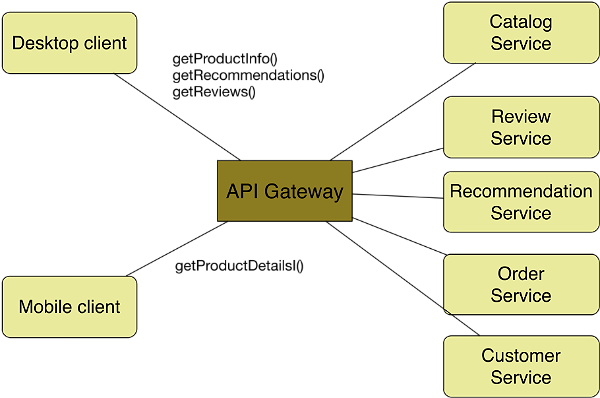
\includegraphics[width=\textwidth,height=\textheight,keepaspectratio,scale=0.1]{images/apigateway1.png}
	\caption{Architettura a microservizi e API Gateway}\label{fig:apig1}
\end{figure}
\newpage
Nella progettazione dell'architettura, il team ha seguito i vincoli posti dall'approccio architetturale \gl{REST}, i quali sono consultabili alla pagina \url{https://en.wikipedia.org/wiki/Representational_state_transfer} (visitato in data 2017-03-26).
\subsection{Sicurezza API Gateway ed endpoints}
Con lo scopo di garantire una certa sicurezza, l'accesso agli endpoints pubblicati sull'API Gateway deve essere controllato e regolato. \\Questo è necessario in quanto tramite essi è possibili fare operazioni sensibili sul sistema, quindi un utente malintenzionato potrebbe comprometterne il corretto funzionamento.\\ 
Il servizio AWS API Gateway fornisce sofisticati ed avanzati meccanismi per la protezione degli endpoint, i quali sono esposti e spiegati alla pagina \url{http://docs.aws.amazon.com/apigateway/latest/developerguide/permissions.html} (visitato in data 2017-03-26). \\

Il sistema progettato prevede due tipologie di utenti (ospite e amministratore), caratterizzati da diverse interazioni con l'assistente virtuale. Vengono quindi supportate dal \file{Back-end} differenti operazioni, invocabili tramite appositi endpoints, in base alla tipologia d'utente. Nasce di conseguenza la necessità di vincolare ogni tipologia d'utente ai soli endpoints ad essa dedicati. \\
Per soddisfare questa esigenza, non sono necessari ulteriori strumenti e meccanismi di AWS API Gateway, in quanto un amministratore è associato ad un \gl{JSON} Web Tokens (JWT) valido. Per capire quindi quali endpoints dovranno essere bloccati all'utente, sarà sufficiente controllare l'esistenza e la validità di questo JWT.
\subsection{Client}
\subsubsection{Client vocale}
L'architettura con la quale è organizzato il client vocale è quella \gl{event-driven}.\\
La motivazione che ha spinto il gruppo a prendere tale decisione è che ciò che dev'essere descritto e realizzato è facilmente modellabile utilizzando questo paradigma. Infatti, ci sono delle componenti che "aspettano" il verificarsi di un evento; altre invece che "notificano"  il verificarsi di un evento.\\
A tal fine, si è fatto utilizzo del pattern comportamentale \gl{Observer}.\\
Ad esempio, la componente \file{Recorder} (che si occupa della registrazione audio), deve prima "aspettare" che qualche individuo parli per potersi attivare, oppure deve "aspettare" che il riproduttore audio abbia terminato la riproduzione prima di potersi rimettere in ascolto.\\
Il client vocale è composto da diverse componenti, le quali sono:
\begin{itemize}
	\item \textbf{Recorder}: questa componente si occupa di realizzare le funzionalità di registrazione. Tramite la classe \file{Utility::BoolObserver}, facente parte del pattern comportamentale Observer utilizzato per modellare ciò, il registratore avrà modo di sapere se il riproduttore audio è in funzione, in maniera tale da non registrare le risposte fornite dal sistema. Una volta terminata la registrazione, il relativo audio verrà inviato alla componente \file{Logic};
	\newpage
	\item \textbf{TTS}: questa componente si occupa di realizzare le funzionalità di text-to-speech, ovvero di riprodurre sotto forma di audio il testo fornito come risposta dall'assistente virtuale. Inoltre, quando la riproduzione audio si attiva/disattiva, le componenti interessate vengono notificate di ciò. Tutto ciò è reso possibile dal pattern comportamentale Observer;
	\item \textbf{ApplicationManager}: questa componente si occupa realizzare le funzionalità di gestione delle applicazioni con le quali l'utente interagisce, permettendo la definizione di esse, la definizione comandi accettati, del salvataggio di stato e del cambio tra un'applicazione e l'altra. Tutto ciò è reso possibile dal pattern \gl{Client-side discovery} riadattato, la quale descrizione è consultabile nell'appendice \ref{CS}. Grazie all'utilizzo del pattern comportamentale Observer, questa componente viene notificata dell'arrivo di dati dal \file{Back-end};
	\item \textbf{ConversationApp}: questa componente si occupa di realizzare l'applicazione ConversationApp, ovvero quella che, tramite interfaccia utente, permette l'interazione con l'assistente virtuale. Per modellare la disposizione delle sue classi, si è fatto utilizzo del pattern Flux descritto nella libreria React, la quale verrà utilizzata per realizzare quanto appena descritto. 
	\item \textbf{Logic}: questa componente si occupa di realizzare le funzionalità che permettono l'interazione, tramite API Gateway, con il \file{Back-end}. Inoltre, quando arrivano dei dati da quest'ultimo, questa componente si occupa di notificare le componenti interessate. Ancora una volta, tutto ciò è organizzato secondo il pattern comportamentale Observer.
\end{itemize}
\subsubsection{Endpoints}
	Ora verranno definiti gli endpoints esterni utilizzati dai vari tipi di client.\\
	Per ogni risorsa sono stati specificati i formati per lo scambio dei dati in JSON:
	\begin{itemize}
		\item \textbf{Request:} rappresenta l’oggetto JSON che dovrà essere passato alla risorsa REST;
		\item \textbf{Response:} rappresenta l’oggetto JSON che fornirà in risposta la risorsa REST.
	\end{itemize}
	L'endpoint utilizzato dal client vocale è:
	\begin{itemize}
		\item \textbf{/query}\\
		\begin{itemize}
			\item \textbf{Method:} POST;
			\item \textbf{Descrizione:} invia all'API Gateway l'audio contenente la richiesta dell'utente;
			\item \textbf{Request:} la richiesta deve contenere i campi organizzati come descritto in \\\file{Back-end::APIGateway::VARequestAPIBody}:
\begin{lstlisting}[language=json,firstnumber=1]
{
 "app":"String",
 "audio":"Base64String",
 "data":"ObjectAssocArray",
 "session_id":"String"
}
\end{lstlisting}
			\item \textbf{Response:} la risposta deve contenere i campi organizzati come descritto in \\\file{Back-end::VirtualAssistant::VAResponse}:
\begin{lstlisting}[language=json,firstnumber=1]
{
"action":"String",
"res":{
 "contexts":"ObjectAssocArray",
 "data":"Object",
 "text_request":"String",
 "text_response":"String"
 },
"session_id":"String"
}
\end{lstlisting}
		\end{itemize}
	\end{itemize}

\subsection{Microservizi}
Di seguito verranno esposti e spiegati i funzionamenti di ogni microservizio da implementare.
\subsubsection{Virtual Assistant}
\paragraph{Descrizione}
Il microservizio Virtual Assistant (VA) fornisce le funzionalità di un assistente virtuale. Fa affidamento ad api.ai, e si occupa di inoltrare le richieste ricevute a tale infrastruttura. Avvalendosi di un database, permette di utilizzare diversi agenti (ciò che trasforma il linguaggio naturale in dati processabili per un'applicazione) durante la stessa interazione, consentendo quindi di definire diverse "applicazioni". Per ogni applicazione, si dovrà definire un agente.\\ Le richieste fatte all'unico endpoint di questo microservizio richiedono infatti di comunicare anche il nome dell'applicazione a cui è legata la richiesta. Questo permette di separare in diversi agenti di api.ai dialoghi legati a diverse funzionalità, affidando la realizzazione e l'integrazione di queste a diversi sviluppatori, senza dover modificare direttamente gli agenti di api.ai. \\
Per avere un completo controllo sul flusso della conversazione, si dovrà fare utilizzo di un database contenente gli agenti utilizzabili, in maniera tale che vengano usati solo quelli definiti e registrati.\\
Il microservizio si occupa anche di notificare, tramite l'utilizzo di AWS SNS, l'avvenuta interazione da parte dell'utente, permettendo così il salvataggio delle conversazioni in un database di supporto, il quale potrebbe essere utilizzato per fini di \gl{machine learning}.\\
Di seguito vengono esposti i vari passaggi affrontati all'arrivo di una richiesta:
\begin{itemize}
	\item arriva una richiesta;
	\item interrogo il database, contenente gli agenti, utilizzando il nome dell'applicazione come chiave;
	\item dall'interrogazione precedente ottengo il token dell'agente relativo all'applicazione;
	\item invio ad api.ai il token, e il testo della richiesta;
	\item api.ai fornisce la risposta, la quale viene "filtrata" da\\ \file{Back-end::VirtualAssistant::ApiAiVAAdapter::query(str: VAQuery): VAResponse}, ottenendo così un formato adatto a \file{Back-end::VirtualAssistant::VAResponse};
	\item pubblico, tramite il servizio Amazon SNS, la risposta filtrata che verrà quindi inviata al Client.
\end{itemize}
\paragraph{Endpoints}

Ora verranno definiti gli Endpoints utilizzati per i passaggi di risorse con il microservizio Virtual Assistant.\\
Per ogni risorsa sono stati specificati i formati per lo scambio dei dati in JSON:
\begin{itemize}
\item \textbf{Request:} rappresenta l’oggetto JSON che dovrà essere passato alla risorsa REST;
\item \textbf{Response:} rappresenta l’oggetto JSON che fornirà in risposta la risorsa REST.
\end{itemize}
Gli Endpoints sono:
\begin{itemize}
\item \textbf{/query}\\
\begin{itemize}
\item \textbf{Method:} POST;
\item \textbf{Descrizione:} invia al microservizio una richiesta per interrogare l'assistente virtuale;
\item \textbf{Request:} la richiesta deve contenere i campi organizzati come descritto in \\\file{Back-end::VirtualAssistant::VAQuery}:
\begin{lstlisting}[language=json,firstnumber=1]
{
 "data":"Object",
 "event":{ /*Alternativo a "text", oggetto di tipo VAEventObject*/
  "data":"Object",
  "name":"String"
 },
 "session_id":"String",
 "text":"String" /*Alternativo a "event"*/
}
\end{lstlisting}
\item \textbf{Response:} la risposta deve contenere i campi organizzati come descritto in \\\file{Back-end::VirtualAssistant::VAResponse}:
\begin{lstlisting}[language=json,firstnumber=1]
{
 "action":"String",
 "res":{/*oggetto di tipo ResponseBody*/
  "contexts":"ObjectAssocArray",
  "data":"Object",
  "text_request":"String",
  "text_response":"String"
 },
 "session_id":"String"
}
\end{lstlisting}
\end{itemize}
\end{itemize}


\subsubsection{Notifications}
\paragraph{Descrizione}
Il microservizio Notifications si occupa di mandare messaggi di notifica nei canali adeguati per notificare gli interessati dell'arrivo di un'ospite in azienda. Fornisce le API per richiedere la lista dei possibili destinatari, e per mandare il messaggio di notifica in un determinato canale. La lista dei canali viene restituita come un'array di stringhe, ognuna delle quali rappresenta un canale.\\
Il microservizio si occupa di interrogare le diverse liste fornite dalla piattaforma di messaggistica scelta e di combinarle in un'unica lista. Nel nostro caso, la piattaforma di messaggistica è \gl{Slack} e le diverse liste fornite riguardano utente, canali e gruppi privati. Quando si vuole mandare un messaggio, il campo \file{Back-end::Notifications::NotificationMessageEvent::send\_to} indica chi è il destinatario di tale messaggio.\\ \file{Back-end::Notifications::NotificationMessageEvent::msg} invece contiene il messaggio vero e proprio, nel formato definito dalla piattaforma di messaggistica su cui si appoggia il microservizio. Il formato utilizzato da Slack è consultabile alla pagina \url{https://api.slack.com/docs/message-buttons} (visitato in data 2017-03-26).
\paragraph{Endpoints}

Ora verranno definiti gli Endpoints utilizzati per i passaggi di risorse con il microservizio Notifications. \\
Per ogni risorsa sono stati specificati i formati per lo scambio dei dati in JSON:
\begin{itemize}
\item \textbf{Request:} rappresenta l’oggetto JSON che dovrà essere passato alla risorsa REST;
\item \textbf{Response:} rappresenta l’oggetto JSON che fornirà in risposta la risorsa REST.
\end{itemize}
Gli Endpoints sono:
\begin{itemize}

\item \textbf{/notifications}\\
\begin{itemize}
\item \textbf{Method:} GET;
\item \textbf{Descrizione:} restituisce la lista dei possibili canali destinatari;
\item \textbf{Response:} la risposta deve contenere i campi organizzati come descritto in \\\file{Back-end::Notifications::NotificationChannel}:
\begin{lstlisting}[language=json,firstnumber=1]
{
  "created": "String",
  "creator": "String",
  "id": "String",
  "is_archived": "boolean",
  "is_member": "boolean",
  "name": "String"
  "num_members": "int",
  "purpose": "Purpose",
  "topic": "Topic",
}
\end{lstlisting}
\end{itemize}

\begin{itemize}
\item \textbf{Method:} POST;
\item \textbf{Descrizione:} invia la notifica ad una determinata persona;
\item \textbf{Request:} la richiesta deve contenere i campi organizzati come descritto in \\\file{Back-end::Notifications::NotificationMsg}:
\begin{lstlisting}[language=json,firstnumber=1]
{
  "msg": [
	"attachments_array":[{},{}], /*Array di Back-end::Notifications::Attachment*/
	"response_type":"String",
	"text":"String"
	],
  "send_to": "String"
}
\end{lstlisting}
\end{itemize}
\end{itemize}

\subsubsection{Users}
\paragraph{Descrizione}
Il microservizio Users si occupa della gestione degli amministratori del nostro sistema. Esso fornisce delle API REST per modificare i dati relativi agli amministratori del nostro sistema presenti in un database. Viene integrato col servizio di Speech Recognition dall'API Gateway, per fornire la possibilità di effettuare il login, tramite impronta vocale, nel sistema.
\paragraph{Endpoints}

Ora verranno definiti gli Endpoints utilizzati per i passaggi di risorse con il microservizio Users. \\
Per ogni risorsa sono stati specificati i formati per lo scambio dei dati in JSON:
\begin{itemize}
\item \textbf{Request:} rappresenta l’oggetto JSON che dovrà essere passato alla risorsa REST;
\item \textbf{Response:} rappresenta l’oggetto JSON che fornirà in risposta la risorsa REST.
\end{itemize}

Gli Endpoints sono:

\begin{itemize}
\item \textbf{/auth/users}\\
\begin{itemize}
\item \textbf{Method:} GET;
\item \textbf{Descrizione:} restituisce la lista degli \file{User} presenti nel database;
\item \textbf{Response:} la risposta deve contenere un array contenente i campi organizzati come descritto in \\\file{Back-end::Auth::User}:
\begin{lstlisting}[language=json,firstnumber=1]
{
  user_array : [
  {
   "first_name":"String",
   "last_name":"String",
   "password":"String",
   "slack_channel":"String",
   "sr_id":"String",
   "username":"String"
  },
  {
   "first_name":"String",
   "last_name":"String",
   "password":"String",
   "slack_channel":"String",
   "sr_id":"String",
   "username":"String"
  },
  {
   "first_name":"String",
   "last_name":"String",
   "password":"String",
   "slack_channel":"String",
   "sr_id":"String",
   "username":"String"
  }
 ]
}
\end{lstlisting}
\end{itemize}

\begin{itemize}
\item \textbf{Method:} POST;
\item \textbf{Descrizione:} vengono inviati i dati necessari all'aggiunta di un nuovo \file{User} al database;
\item \textbf{Request:} la richiesta deve contenere i campi organizzati come descritto in\\ \file{Back-end::Auth::User}:
\begin{lstlisting}[language=json,firstnumber=1]
{
  "first_name":"String",
  "last_name":"String",
  "password":"String",
  "slack_channel":"String",
  "sr_id":"String",
  "username":"String"
}
\end{lstlisting}
\item \textbf{Response}: il corpo della risposta sarà vuoto, ma il risultato di questa operazione sarà comunque deducibile dal valore dello status code \gl{HTTP};
\end{itemize}

\item \textbf{/auth/users/:username}\\

\begin{itemize}
\item \textbf{Method:} PUT;
\item \textbf{Descrizione:} vengono modificati i dati dell'utente, il quale identificativo è specificato nel path, tramite sovrascrittura;
\item \textbf{Request:} la richiesta deve contenere i campi organizzati come descritto in \\\file{Back-end::Auth::User}
\begin{lstlisting}[language=json,firstnumber=1]
{
  "first_name":"String",
  "last_name":"String",
  "password":"String",
  "slack_channel":"String",
  "sr_id":"String",
  "username":"String"
}
\end{lstlisting}
\item \textbf{Response}: il corpo della risposta sarà vuoto, ma il risultato di questa operazione sarà comunque deducibile dal valore dello status code HTTP.
\end{itemize}

\begin{itemize}
\item \textbf{Method:} DELETE;
\item \textbf{Descrizione:} viene eliminato un utente, il quale identificativo è specificato nel path;
\item \textbf{Response}: il corpo della risposta sarà vuoto, ma il risultato di questa operazione sarà comunque deducibile dal valore dello status code HTTP;
\end{itemize}

\begin{itemize}
\item \textbf{Method:} GET;
\item \textbf{Descrizione:} vengono ricevuti i dati relativi ad un utente, il quale identificativo è specificato nel path;
\item \textbf{Response:} la risposta deve contenere i campi organizzati come descritto in \\\file{Back-end::Auth::User}:
\begin{lstlisting}[language=json,firstnumber=1]
{
  "first_name":"String",
  "last_name":"String",
  "password":"String",
  "slack_channel":"String",
  "sr_id":"String",
  "username":"String"
}
\end{lstlisting}
\end{itemize}

\end{itemize}

\subsubsection{Rules}
\paragraph{Descrizione}
Il microservizio Rules si occupa della gestione delle \gl{direttive} del sistema. Una direttiva è un'istruzione che viene data da un amministratore al sistema, la quale permette di modificare il comportamento del sistema stesso al verificarsi di certe condizioni. Tali condizioni possono essere legate alla persona che interagisce col sistema, la sua azienda di provenienza, oppure alla persona desiderata che viene richiesta.\\
Il sistema fornisce una serie di funzioni per modificare il suo comportamento, le quali indicano il modo in cui esso debba essere cambiato. \\
Una direttiva è costituita da:
\begin{itemize}
	\item una lista di target, che indica gli obiettivi (persone) ai quali deve essere applicata la direttiva;
	\item un'istanza di funzione, che indica quale delle funzioni disponibili deve essere applicata e, nel caso in cui tale funzione abbia dei parametri modificabili, con quali valori di quest'ultimi deve essere chiamata;
	\item un nome, il quale permette agli amministratori di identificare le diverse direttive;
	\item un id, il quale identifica univocamente la funzione all'interno del sistema;
	\item una flag di abilitazione, che permette di abilitare e disabilitare l'applicazione della direttiva da parte del sistema.
\end{itemize}

\paragraph{Endpoints}

Ora verranno definiti gli Endpoints utilizzati per i passaggi di risorse con il microservizio Rules.\\
Per ogni risorsa sono stati specificati i formati per lo scambio dei dati in JSON:
\begin{itemize}
\item \textbf{Request:} rappresenta l’oggetto JSON che dovrà essere passato alla risorsa REST;
\item \textbf{Response:} rappresenta l’oggetto JSON che fornirà in risposta la risorsa REST.
\end{itemize}
Gli Endpoints sono:

\begin{itemize}

\item \textbf{/impostazioni}\\

\begin{itemize}
\item \textbf{Method:} GET;
\item \textbf{Descrizione:} viene ricevuta la lista delle direttive;
\item \textbf{Response:} la risposta deve contenere un array contenente i campi organizzati come descritto in \\\file{Back-end::Rules::Rule}:
\begin{lstlisting}[language=json,firstnumber=1]
{
 rule_array : [
 {
  "ac_list":[
	"adm1":"String",
	"adm2":"String",
	...
   ],
  "ac_mode":"int",
  "enabled":"boolean",
  "id":"int",
  "name":"String",
  "targets":[ /*oggetti di tipo Back-end::Rules::RuleTarget*/
  {
   "company":"String",
   "member":"String",
   "name":"String"
  },
  {
   "company":"String",
   "member":"String",
   "name":"String"
  }
  ],
  "task":{ /* oggetto di tipo Back-end::Rules::RuleTaskInstance*/
   "params":{
	"par1":"Object",
	"par2":"Object",
	...
   }
   "task":"String"
  }
 }
 ]
}
\end{lstlisting}
\end{itemize}

\begin{itemize}
\item \textbf{Method:} POST;
\item \textbf{Descrizione:} viene creata una nuova direttiva;
\item \textbf{Request:} la richiesta deve contenere i campi organizzati come descritto in \\\file{Back-end::Rules::Rule}:
\begin{lstlisting}[language=json,firstnumber=1]
{
	rule : {
	  "ac_list":[
	    "adm1":"String",
	    "adm2":"String",
		...
	  ],
	  "ac_mode":"int",
	  "enabled":"boolean",
	  "id":"int",
	  "name":"String",
	  "targets":[ /* oggetti di tipo Back-end::Rules::RuleTarget */
	  {
		"company":"String",
		"member":"String",
		"name":"String"
      },
	  {
		"company":"String",
		"member":"String",
		"name":"String"
	  }
	  ],
	  "task":{ /* oggetto di tipo Back-end::Rules::RuleTaskInstance*/
		"params":{
		  "par1":"Object",
		  "par2":"Object",
		  ...
	   }
	  "task":"String"
	  }
	}
}
\end{lstlisting}
\item \textbf{Response}: il corpo della risposta sarà vuoto, ma il risultato di questa operazione sarà comunque deducibile dal valore dello status code HTTP;
\end{itemize}

\item \textbf{/impostazioni/:id}\\

\begin{itemize}
\item \textbf{Method:} PUT;
\item \textbf{Descrizione:} viene modificata una direttiva, il quale identificativo è specificato nel path, tramite sovrascrittura;
\item \textbf{Request:} la richiesta deve contenere i campi organizzati come descritto in \\\file{Back-end::Rules::Rule}:
\begin{lstlisting}[language=json,firstnumber=1]
{
  rule : {
	"ac_list":[
	 "adm1":"String",
	 "adm2":"String",
	...
    ],
	"ac_mode":"int",
	"enabled":"boolean",
	"id":"int",
	"name":"String",
	"targets":[ /* oggetti di tipo Back-end::Rules::RuleTarget */
	{
	 "company":"String",
	 "member":"String",
	 "name":"String"
	},
	{
	 "company":"String",
	 "member":"String",
	 "name":"String"
	}
	],
	"task":{ /* oggetto di tipo Back-end::Rules::RuleTaskInstance*/
	 "params":{
	  "par1":"Object",
	  "par2":"Object",
	  ...
	 }
	"task":"String"
   }
  }
}
\end{lstlisting}
\item \textbf{Response}: il corpo della risposta sarà vuoto, ma il risultato di questa operazione sarà comunque deducibile dal valore dello status code HTTP;
\end{itemize}

\begin{itemize}
\item \textbf{Method:} GET;
\item \textbf{Descrizione:} vengono richiesti dati relativi ad una specifica direttiva, il quale identificativo è specificato nel path;
\item \textbf{Response:} la risposta deve contenere i campi organizzati come descritto in \\\file{Back-end::Rules::Rule}:
\begin{lstlisting}[language=json,firstnumber=1]
{
	rule : {
	 "ac_list":[
	  "adm1":"String",
	  "adm2":"String",
	  ...
	  ],
	"ac_mode":"int",
	"enabled":"boolean",
	"id":"int",
	"name":"String",
	"targets":[ /* oggetti di tipo Back-end::Rules::RuleTarget */
	{
	 "company":"String",
	 "member":"String",
	 "name":"String"
	},
	{
	 "company":"String",
	 "member":"String",
	 "name":"String"
	}
	],
	"task":{ /* oggetto di tipo Back-end::Rules::RuleTaskInstance*/
	 "params":{
	  "par1":"Object",
	  "par2":"Object",
	  ...
	 }
	"task":"String"
	}
  }
}
\end{lstlisting}

\end{itemize}

\begin{itemize}
\item \textbf{Method:} DELETE;
\item \textbf{Descrizione:} viene eliminata una direttiva, il quale identificativo è specificato nel path;
\item \textbf{Response}: il corpo della risposta sarà vuoto, ma il risultato di questa operazione sarà comunque deducibile dal valore dello status code HTTP;
\end{itemize}


\item \textbf{/impostazioni/tasks}\\

\begin{itemize}
\item \textbf{Method:} GET;
\item \textbf{Descrizione:} viene richiesta la lista dei tipi di funzioni presenti nel sistema;
\item \textbf{Response:} la risposta deve contenere i campi organizzati come descritto in \\\file{Back-end::Rules::Task}:
\begin{lstlisting}[language=json,firstnumber=1]
{
 function_array : [
 {
  "function":"String",
  "id":"int"
 },
 {
  "function":"String",
  "id":"int"
 }
]
}
\end{lstlisting}
\end{itemize}

\begin{itemize}
\item \textbf{Method:} POST;
\item \textbf{Descrizione:} viene creato un nuovo tipo di \file{Task};
\item \textbf{Request:} la richiesta deve contenere i campi organizzati come descritto in \\\file{Back-end::Rules::Task}:
\begin{lstlisting}[language=json,firstnumber=1]
{
 function_array : [
 {
  "function":"String",
  "id":"int"
 },
 {
  "function":"String",
  "id":"int"
 }
 ]
}
\end{lstlisting}
\item \textbf{Response}: il corpo della risposta sarà vuoto, ma il risultato di questa operazione sarà comunque deducibile dal valore dello status code HTTP.
\end{itemize}



\item \textbf{/impostazioni/tasks/:type}\\

\begin{itemize}
\item \textbf{Method:} GET;
\item \textbf{Descrizione:} viene richiesto un \file{Task} in base al tipo di funzione applicata, , il quale identificativo è specificato nel path;

\item \textbf{Response:} la risposta deve contenere i campi organizzati come descritto in \\\file{Back-end::Rules::Task}:
\begin{lstlisting}[language=json,firstnumber=1]
{
 function_array : [
 {
  "function":"String",
  "id":"int"
 },
 {
  "function":"String",
  "id":"int"
 }
 ]
}
\end{lstlisting}
\end{itemize}

\begin{itemize}
\item \textbf{Method:} PUT;
\item \textbf{Descrizione:} viene modificata un \file{Task}, il quale identificativo è specificato nel path tramite sovrascrittura;
\item \textbf{Request:} la richiesta deve contenere i campi organizzati come descritto in \\\file{Back-end::Rules::Task}:
\begin{lstlisting}[language=json,firstnumber=1]
{
 function_array : [
 {
  "function":"String",
  "id":"int"
 },
 {
  "function":"String",
  "id":"int"
 }
 ]
}
\end{lstlisting}
\item \textbf{Response}: il corpo della risposta sarà vuoto, ma il risultato di questa operazione sarà comunque deducibile dal valore dello status code HTTP.
\end{itemize}

\end{itemize}
\newpage
\subsection{Action supportate} \label{action}
Di seguito vengono elencate le action, supportate dal \file{Back-end}, che api.ai può ritornare in seguito alla richiesta di un utente. \\
Una action è una stringa che indica quale operazione dovrà essere scelta dall'API Gateway, in modo da soddisfare le richieste dell'utente.\\
I metodi citati appartengono alla classe \file{Back-end::APIGateway::VocalAPI}.
\subsubsection{User}
\begin{itemize}
\item \file{user.add}: utilizza il metodo privato \file{addUser(user: User)} per aggiungere un utente registrato, cioè un amministratore, al sistema;

\item \file{user.get}: utilizza il metodo privato \file{getUser(username: String)} per ottenere i dati relativi ad un utente registrato;

\item \file{user.getList}: utilizza il metodo privato \file{getUserList()} per ottenere la lista degli utenti registrati; 

\item \file{user.update}: utilizza il metodo privato \file{updateUser(user: User)} per aggiornare un utente registrato;

\item \file{user.remove}: utilizza il metodo privato \file{removeUser(username: String)} per rimuovere un utente registrato;

\item \file{user.addEnrollment}: utilizza il metodo privato \file{addUserEnrollment(enr: Enrollment)} per aggiungere un Enrollment ad un utente registrato;

\item \file{user.resetEnrollments}: utilizza il metodo privato \file{resetUserEnrollment(username: String):} per resettare gli Enrollment relativi ad un utente registrato;

\item \file{user.login}: utilizza il metodo privato \file{loginUser(enr: Enrollment)} per effettura il login di un utente registrato.

\end{itemize}
\subsubsection{Rule}
\begin{itemize}
\item \file{rule.add}: utilizza il metodo privato \file{addRule(rule: Rule)} per aggiungere una direttiva;

\item \file{rule.get}: utilizza il metodo privato \file{getRule(id: String)} per ottenere i dati relativi una direttiva;

\item \file{rule.getList}: utilizza il metodo privato \file{getRuleList()} per ottenere la lista delle direttive;

\item \file{rule.update}: utilizza il metodo privato \file{updateRule(rule: Rule)} per aggiornare una direttiva;

\item \file{rule.remove}: utilizza il metodo privato \file{removeRule(id: String)} per rimuovere una direttiva.


\end{itemize}


	\section{Specifica delle Componenti}
\subsection{Back-end}
Package contenente tutte le componenti che costituiscono il back-end. Le componenti sono organizzate secondo il pattern a microservizi.
\subsubsection{Classi}
\hypertarget{ ConversationsDAO_label}{\paragraph{ ConversationsDAO}}
\begin{figure}[h]
	\centering
	\includegraphics[width=\textwidth,height=\textheight,keepaspectratio]{images/Class ConversationsDAO.png}
	\caption{Back-end:: ConversationsDAO}
\end{figure}
\begin{itemize}
	\item \textbf{Nome}: \file{ ConversationsDAO};
	\item \textbf{Tipo}: \file{Interface};
	\item \textbf{Descrizione}: questa classe si occupa di astrarre le modalità d'interazione al database contenente le conversazioni;
	\item \textbf{Utilizzo}: fornisce a \file{ConversationWebhookService} un meccanismo per accedere al database contenente le conversazioni, senza conoscerne le modalità di implementazioni e di persistenza di quest'ultimo. Permette operazioni di lettura, scrittura e rimozione di utenti registrati;
	\item \textbf{Attributi}:
	\begin{itemize}
		\item[] \file{- db: AWS::DynamoDB} \\
		Attributo che permette di contattare il database contenente le conversazioni;
		\item[] \file{- guest\_id: String} \\
		Attributo contenente l'id dell'ospite identificato;
	\end{itemize}
	\item \textbf{Metodi}:
	\begin{itemize}
		\item[] \file{+ getConversationList(): ConversationObservable} \\
		L'\file{Observable} restituito manderà agli \file{Observer} le conversazioni ottenute, uno alla volta, e poi chiama il loro metodo \file{complete}. Nel caso in cui si verifichi un errore, gli \file{Observer} iscritti verranno notificati tramite la chiamate del loro metodo \file{error} con i dati relativi all'errore verificatosi;\\
		\item[] \file{+ getConversation(session\_id: String, timestamp: String): ConversationObservable} \\
		Metodo che permette di ottenere una conversazione a partire dall'identificativo della sessione e dal suo timestamp. \\ L'\file{Observable} restituito riceverà l'oggetto rappresentante tale \file{Conversation}, e verrà completato. Nel caso in cui la conversazione richiesta non sia presente nel database, gli \file{Observer} interessati non riceveranno alcun valore, ma verranno notificati tramite la chiamata del loro metodo \file{error()};\\
		Parametri:
		\begin{itemize}
			\item \file{session\_id: String} \\
			Parametro contenente l'id della sessione della conversazione da ricevere;
			\item \file{timestamp: String} \\
			Parametro contenente il timestamp relativo all'inizio della conversazione;
		\end{itemize}
		\item[] \file{+ addConversation(conversation: Conversation): ErrorObservable} \\
		Metodo che permette di aggiungere una conversazione al database.  L'\file{Observable} restituito non riceverà alcun valore, ma verrà completato in caso di aggiunta della conversazione avvenuta con successo. In caso di errore durante l'aggiunta della conversazione, gli \file{Observer} interessati verranno notificati tramite la chiamata del loro metodo \file{error()} con i dati relativi all'errore verificatosi;\\
		Parametri:
		\begin{itemize}
			\item \file{conversation: Conversation} \\
			Parametro contente la conversazione da inserire;
		\end{itemize}
		\item[] \file{+ addMessage(msg: ConversationMessage, timestamp: String, session\_id: String): ErrorObservable} \\
		Metodo che permette di aggiungere un messaggio relativo ad una conversazione al database a partire da un messaggio, un timestamp relativo e l'identificativo della relativa conversazione.  L'\file{Observable} restituito non riceverà alcun valore, ma verrà completato in caso di aggiunta del messaggio avvenuta con successo. In caso di errore durante l'aggiunta del messaggio, gli \file{Observer} interessati verranno notificati tramite la chiamata del loro metodo \file{error()} con i dati relativi all'errore verificatosi;\\
		Parametri:
		\begin{itemize}
			\item \file{msg: ConversationMessage} \\
			Parametro contenente il messaggio;
			\item \file{timestamp: String} \\
			Parametro contenente il timestamp relativo all'inizio della conversazione;
			\item \file{session\_id: String} \\
			Parametro contenente l'id della sessione della conversazione alla quale aggiungere il messaggio;
		\end{itemize}
		\item[] \file{+ removeConversation(session\_id: String, timestamp: String): ErrorObservable} \\
		Metodo che permette di rimuovere una conversazione a partire dall'identificativo della sessione e dal suo timestamp.  L'\file{Observable} restituito non riceverà alcun valore, ma verrà completato in caso di aggiunta della conversazione avvenuta con successo. In caso di errore durante l'aggiunta della conversazione, gli \file{Observer} interessati verranno notificati tramite la chiamata del loro metodo \file{error()} con i dati relativi all'errore verificatosi;\\
		Parametri:
		\begin{itemize}
			\item \file{session\_id: String} \\
			Parametro contenente l'id della sessione della conversazione da eliminare;
			\item \file{timestamp: String} \\
			Parametro contenente il timestamp del messaggio da eliminare;
		\end{itemize}
	\end{itemize}
\end{itemize}

\hypertarget{ GuestsDAO_label}{\paragraph{ GuestsDAO}}
\begin{figure}[h]
	\centering
	\includegraphics[width=\textwidth,height=\textheight,keepaspectratio]{images/Class GuestsDAO.png}
	\caption{Back-end:: GuestsDAO}
\end{figure}
\begin{itemize}
	\item \textbf{Nome}: \file{ GuestsDAO};
	\item \textbf{Tipo}: \file{Interface};
	\item \textbf{Descrizione}: questa interfaccia si occupa di astrarre le modalità d'interazione al database contenente gli ospiti conosciuti;
	\item \textbf{Utilizzo}: fornisce i metodi per accedere al database contenente i dati relativi agli ospiti conosciuti, senza conoscerne le modalità di implementazioni e di persistenza di quest'ultimo. Permette operazioni di lettura, scrittura e rimozione di ospiti conosciuti;
	\item \textbf{Attributi}:
	\begin{itemize}
		\item[] \file{- db: AWS::DynamoDB} \\
		Attributo contenente;
	\end{itemize}
	\item \textbf{Metodi}:
	\begin{itemize}
		\item[] \file{+ getGuestList(): GuestObservable} \\
		L'\file{Observable} restituito manderà agli \file{Observer} gli ospiti ottenuti, uno alla volta, e poi chiama il loro metodo \file{complete}. Nel caso in cui si verifichi un errore, gli \file{Observer} iscritti verranno notificati tramite la chiamate del loro metodo \file{error} con i dati relativi all'errore verificatosi;\\
		\item[] \file{+ getGuest(name: String, company: String): GuestObservable} \\
		Metodo che permette di ottenere un ospite a partire dal nome e l'azienda di provenienza. \\
L'\file{Observable} restituito riceverà l'oggetto rappresentante tale \file{Guest}, e verrà completato. Nel caso in cui l'ospite richiesto non sia presente nel database, gli \file{Observer} interessati non riceveranno alcun valore, ma verranno notificati tramite la chiamata del loro metodo \file{error()};\\
		Parametri:
		\begin{itemize}
			\item \file{name: String} \\
			Parametro contenente il nome dell'ospite;
			\item \file{company: String} \\
			Parametro contenente l'azienda di provenienza dell'ospite;
		\end{itemize}
		\item[] \file{+ updateGuest(guest: Guest): ErrorObservable} \\
		Metodo che permette di aggiornare un ospite.  L'\file{Observable} restituito non riceverà alcun valore, ma verrà completato in caso di aggiunta dell'ospite avvenuta con successo. In caso di errore durante l'aggiunta dell'ospite, gli \file{Observer} interessati verranno notificati tramite la chiamata del loro metodo \file{error()} con i dati relativi all'errore verificatosi;\\
		Parametri:
		\begin{itemize}
			\item \file{guest: Guest} \\
			Parametro contenente l'ospite da aggiornare;
		\end{itemize}
		\item[] \file{+ removeGuest(name: String, company: String): ErrorObservable} \\
		Metodo che permette di eliminare un ospite dal database, a partire dal suo nome e azienda di provenienza.  L'\file{Observable} restituito non riceverà alcun valore, ma verrà completato in caso di eliminazione  dell'ospite avvenuta con successo. In caso di errore durante l'eliminazione dell'ospite, gli \file{Observer} interessati verranno notificati tramite la chiamata del loro metodo \file{error()} con i dati relativi all'errore verificatosi;\\
		Parametri:
		\begin{itemize}
			\item \file{name: String} \\
			Parametro contenente il nome dell'ospite;
			\item \file{company: String} \\
			Parametro contenente l'azienda di provenienza dell'ospite;
		\end{itemize}
		\item[] \file{+ addGuest(guest: Guest): ErrorObservable} \\
		Metodo che permette di aggiungere un ospite al database.  L'\file{Observable} restituito non riceverà alcun valore, ma verrà completato in caso di aggiunta dell'ospite avvenuta con successo. In caso di errore durante l'aggiunta dell'ospite, gli \file{Observer} interessati verranno notificati tramite la chiamata del loro metodo \file{error()} con i dati relativi all'errore verificatosi;\\
		Parametri:
		\begin{itemize}
			\item \file{guest: Guest} \\
			Parametro contenente l'ospite da aggiungere;
		\end{itemize}
	\end{itemize}
\end{itemize}

\hypertarget{AdministrationWebhookService_label}{\paragraph{AdministrationWebhookService}}
\begin{figure}[h]
	\centering
	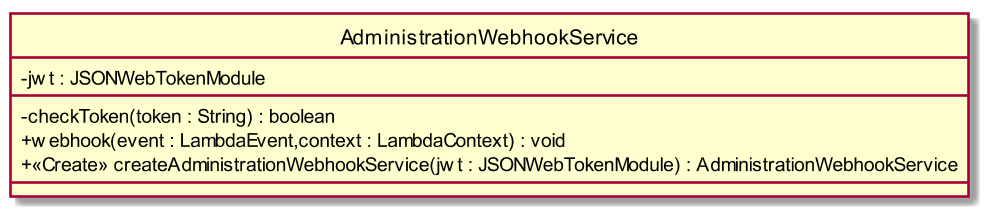
\includegraphics[width=\textwidth,height=\textheight,keepaspectratio]{images/ClassAdministrationWebhookService.png}
	\caption{Back-end::AdministrationWebhookService}
\end{figure}
\begin{itemize}
	\item \textbf{Nome}: \file{AdministrationWebhookService};
	\item \textbf{Tipo}: \file{Class};
	\item \textbf{Descrizione}: questa classe si occupa di implementare l'interfaccia \file{WebhookService}, realizzando un Webhook che fornisce una risposta all'Agent di amministrazione;
	\item \textbf{Utilizzo}: fornisce il metodo che si occupa di rispondere alle chiamate al microservizio da parte dell'Agent di amministrazione;
	\item \textbf{Padre}: \file{<<interface>> WebhookService};
	\item \textbf{Attributi}:
	\begin{itemize}
		\item[] \file{- rules: RulesDAO} \\
		Attributo che permette di contattare \file{RulesDAO}, il quale fornisce i meccanismi di accesso al database contenente le \file{Rule};
		\item[] \file{- users: UsersDAO} \\
		Attributo che permette di contattare \file{UsersDAO}, il quale fornisce i meccanismi di accesso al database contenente gli utenti registrati;
	\end{itemize}
	\item \textbf{Metodi}:
	\begin{itemize}
		\item[] \file{- checkToken(token: String): boolean} \\
		Metodo che permette di controllare l'autenticità di un JWT. Utilizzato dal metodo webhook per controllare che la richiesta sia stata fatta da un amministratore autenticato prima di compiere qualsiasi altra azione;\\
		Parametri:
		\begin{itemize}
			\item \file{token: String} \\
			Parametro contenente il JWT per l'autenticazione;
		\end{itemize}
		\item[] \file{+ webhook(event: LambdaEvent, context: LambdaContext): void} \\
		Questo metodo soddisfa i requisiti per webhook descritti da api.ai. Viene chiamato ad ogni interazione dell'agente di amministrazione, e per prima cosa si occupa di verificare che nella richiesta sia presente un JSON Web Token (JWT) che confermi un'autenticazione avvenuta con successo. In caso di mancata autenticazione, lo stato della risposta sarà impostato a 403.  Nel caso in cui il token sia presente e valido (la firma sia valida ed il token non sia scaduto), si occupa di eseguire l'operazione richiesta dall'assistente virtuale. Tale operazione è specificata in fulfillment.messages (vedi classi \file{ProcessingResult}, \file{Fullfillement} e \file{MsgObject} per eventuali chiarimenti riguardanti il formato della richiesta fatta da api.ai al microservizio). In particolare, all'interno di \file{messages} sarà presente un messaggio con \file{type=4}, il quale relativo attributo \file{payload} consisterà in un oggetto di tipo \file{WebhookCmd}. In base al campo \file{cmd} di tale oggetto questo metodo interpreterà il formato del campo \file{params}, ricavando i parametri necessari ad eseguire il comando specificato e poi eseguendo l'azione richiesta. In caso di successo verrà richiesto all'utente se vuole compiere qualche altra azione utilizzando il campo speech dell'oggeto \file{WebhookResponse} utilizzato per rispondere. In caso di mancanza del comando (nessun messaggio con \file{type=4} in \file{fulfillment.messages}), il campo speech della risposta sarà copiato da \file{fulfillment.speech} della richiesta, risultando quindi in una risposta uguale a quella fornita da api.ai in assenza di webhook;\\
		Parametri:
		\begin{itemize}
			\item \file{event: LambdaEvent} \\
			Parametro contenente;
			\item \file{context: LambdaContext} \\
			Parametro contenente;
		\end{itemize}
		\item[] \file{+ <<Create>> createAdministrationWebhookService(rulesdao: RulesDAO, usersdao: UsersDAO): AdministrationWebhookService} \\
		zzz;\\
		Parametri:
		\begin{itemize}
			\item \file{rulesdao: RulesDAO} \\
			Attributo contenente il \file{RulesDAO};
			\item \file{usersdao: UsersDAO} \\
			Attributo contenente lo \file{UsersDAO};
		\end{itemize}
	\end{itemize}
\end{itemize}

\hypertarget{AgentObservable_label}{\paragraph{AgentObservable}}
\begin{figure}[h]
	\centering
	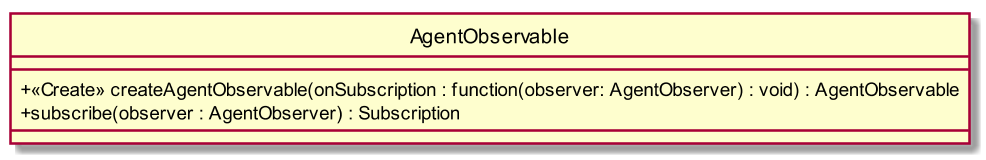
\includegraphics[width=\textwidth,height=\textheight,keepaspectratio]{images/ClassAgentObservable.png}
	\caption{Back-end::AgentObservable}
\end{figure}
\begin{itemize}
	\item \textbf{Nome}: \file{AgentObservable};
	\item \textbf{Tipo}: \file{Class};
	\item \textbf{Descrizione}: questa classe implementa un \file{Observable} che permette l'iscrizione di \file{AgentObserver};
	\item \textbf{Utilizzo}: fornisce i meccanismi necessari per il passaggio di una serie di \file{Agent} ad un \file{Observer} interessato;
	\item \textbf{Padre}: \file{Observable};
	\item \textbf{Metodi}:
	\begin{itemize}
		\item[] \file{+ <<Create>> createAgentObservable(onSubscription: function(observer: AgentObserver) : void): AgentObservable} \\
		Constructor di \file{AgentObservable};\\
		Parametri:
		\begin{itemize}
			\item \file{onSubscription: function(observer: AgentObserver) : void} \\
			Funzione che verrà eseguita quando un \file{Observer} si iscrive all'\file{Observable}. Si occupa di passare i dati all'\file{Observer}, chiamando il metodo \file{next(agent: Agent)}. Quando non ci sono più dati da restituire, si occupa di chiamare il metodo \file{complete()}. Nel caso in cui si verificasse un errore, si occupa di chiamare il metodo \file{error(err: Object)} con i dati relativi all'errore verificatosi;
		\end{itemize}
		\item[] \file{+ subscribe(observer: AgentObserver): Subscription} \\
		Metodo che permette ad uno \file{AgentObserver} interessato di iscriversi a questo \file{Observable};\\
		Parametri:
		\begin{itemize}
			\item \file{observer: AgentObserver} \\
			\file{Observer} che si vuole iscrivere;
		\end{itemize}
	\end{itemize}
\end{itemize}

\hypertarget{AgentObserver_label}{\paragraph{AgentObserver}}
\begin{figure}[h]
	\centering
	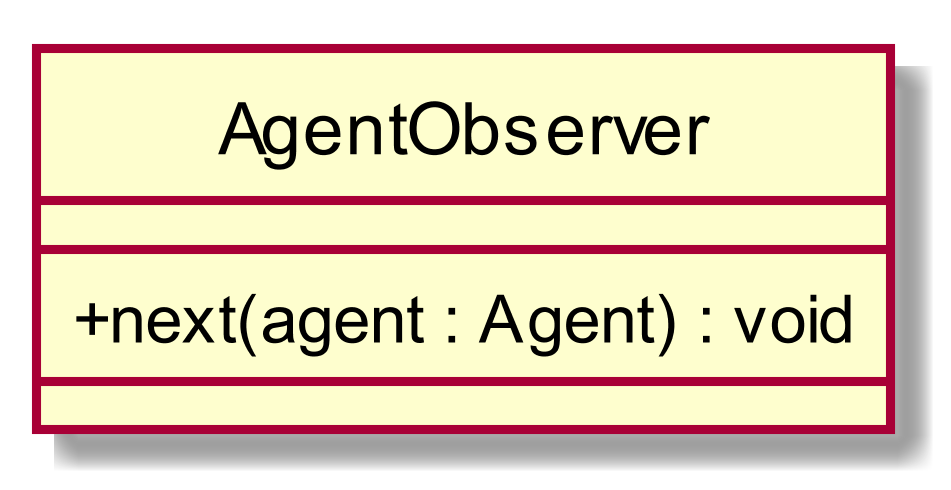
\includegraphics[width=\textwidth,height=\textheight,keepaspectratio]{images/ClassAgentObserver.png}
	\caption{Back-end::AgentObserver}
\end{figure}
\begin{itemize}
	\item \textbf{Nome}: \file{AgentObserver};
	\item \textbf{Tipo}: \file{Class};
	\item \textbf{Descrizione}: classe che rappresenta un \file{Observer} che si aspetta dati di tipo \file{Agent};
	\item \textbf{Utilizzo}: implementa il metodo \file{next()} dell'interfaccia, in maniera tale che accetti dati di tipo \file{Agent};
	\item \textbf{Metodi}:
	\begin{itemize}
		\item[] \file{+ next(agent: Agent): void} \\
		Metodo che permette agli \file{Observable} di notificare l'\file{Observer} con dati di tipo \file{Agent}. Definisce inoltre le operazioni che l'\file{Observer} compierà all'arrivo di tali dati;\\
		Parametri:
		\begin{itemize}
			\item \file{agent: Agent} \\
			Parametro contenente l'\file{Agent} mandato dall'\file{Observable};
		\end{itemize}
	\end{itemize}
\end{itemize}

\hypertarget{Conversation_label}{\paragraph{Conversation}}
\begin{figure}[h]
	\centering
	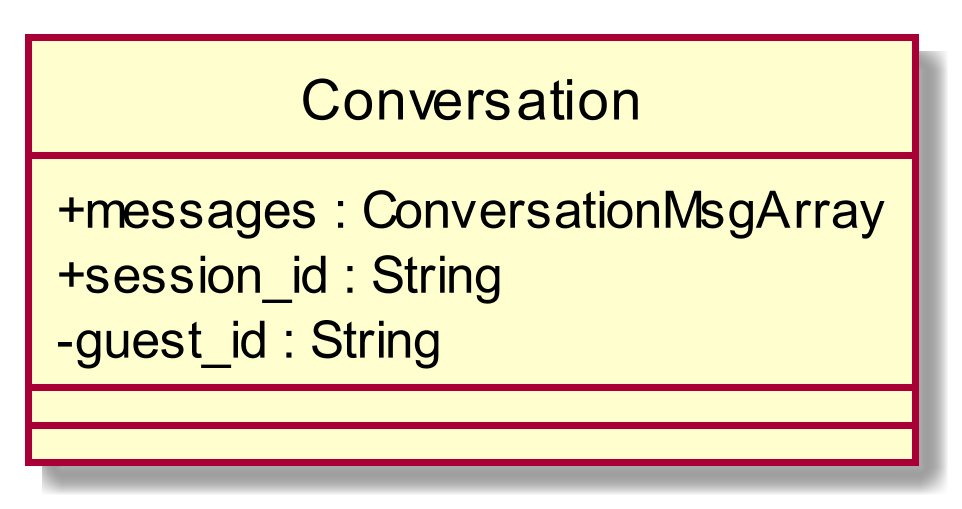
\includegraphics[width=\textwidth,height=\textheight,keepaspectratio]{images/ClassConversation.png}
	\caption{Back-end::Conversation}
\end{figure}
\begin{itemize}
	\item \textbf{Nome}: \file{Conversation};
	\item \textbf{Tipo}: \file{Class};
	\item \textbf{Descrizione}: questa classe si occupa di rappresentare e organizzare gli attributi relativi ad una conversazione, la quale dovrà essere salvata nel database;
	\item \textbf{Utilizzo}: fornisce gli attributi relativi ad una conversazione;
	\item \textbf{Attributi}:
	\begin{itemize}
		\item[] \file{+ messages: ConversationMsgArray} \\
		Attributo contenente l'array dei messaggi contenuti in una conversazione;
		\item[] \file{+ session\_id: String} \\
		Attributo contenente l'id della sessione relativa alla conversazione;
		\item[] \file{+ timestamp: String} \\
		Attributo contenente il timestamp relativo alla conversazione. Tutti i messaggi di una conversazione  hanno lo stesso timestamp, il quale indica l'inizio della conversazione;
	\end{itemize}
\end{itemize}

\hypertarget{ConversationMsg_label}{\paragraph{ConversationMsg}}
\begin{figure}[h]
	\centering
	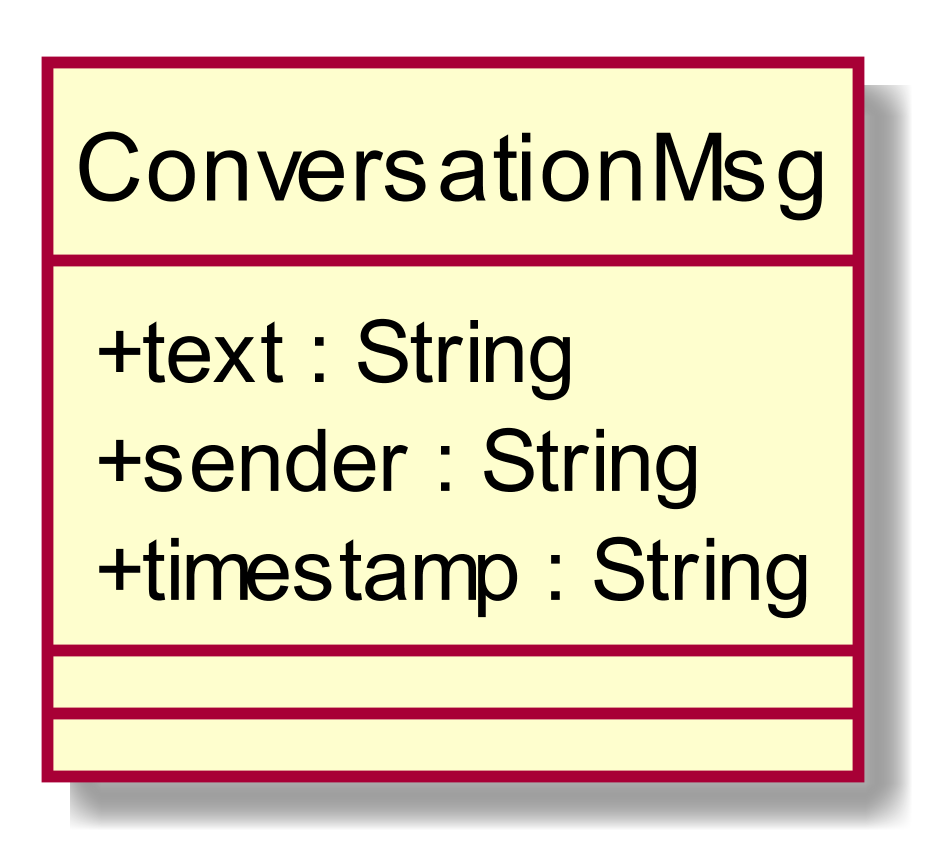
\includegraphics[width=\textwidth,height=\textheight,keepaspectratio]{images/ClassConversationMsg.png}
	\caption{Back-end::ConversationMsg}
\end{figure}
\begin{itemize}
	\item \textbf{Nome}: \file{ConversationMsg};
	\item \textbf{Tipo}: \file{Class};
	\item \textbf{Descrizione}: questa classe si occupa di rappresentare e organizzare gli attributi relativi ad un messaggio all'interno di una conversazione;
	\item \textbf{Utilizzo}: fornisce gli attributi relativi un messaggio. La classe \file{Conversation} contiene un array di essi, in modo da costruire l'intera conversazione;
	\item \textbf{Attributi}:
	\begin{itemize}
		\item[] \file{+ text: String} \\
		Attributo contenente il testo del messaggio;
		\item[] \file{+ sender: String} \\
		Attributo contenente il mittente del messaggio;
		\item[] \file{+ timestamp: String} \\
		Attributo contenente il timestamp del messaggio;
	\end{itemize}
\end{itemize}

\hypertarget{ConversationObservable_label}{\paragraph{ConversationObservable}}
\begin{figure}[h]
	\centering
	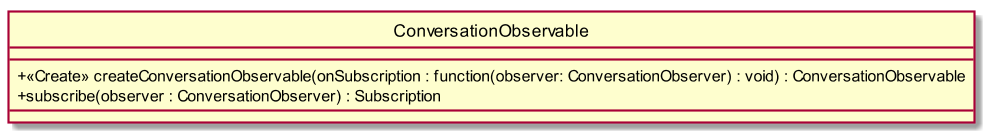
\includegraphics[width=\textwidth,height=\textheight,keepaspectratio]{images/ClassConversationObservable.png}
	\caption{Back-end::ConversationObservable}
\end{figure}
\begin{itemize}
	\item \textbf{Nome}: \file{ConversationObservable};
	\item \textbf{Tipo}: \file{Class};
	\item \textbf{Descrizione}: questa classe implementa un \file{Observable} che permette l'iscrizione di \file{ConversationObserver};
	\item \textbf{Utilizzo}: fornisce i meccanismi necessari per il passaggio di una serie di \file{Conversation} ad un \file{Observer} interessato;
	\item \textbf{Padre}: \file{Observable};
	\item \textbf{Metodi}:
	\begin{itemize}
		\item[] \file{+ <<Create>> createConversationObservable(onSubscription: function(observer: ConversationObserver) : void): ConversationObservable} \\
		Constructor di \file{ConversationObservable};\\
		Parametri:
		\begin{itemize}
			\item \file{onSubscription: function(observer: ConversationObserver) : void} \\
			Funzione che verrà eseguita quando un \file{Observer} si iscrive all'\file{Observable}. Si occupa di passare i dati all'\file{Observer}, chiamando il metodo \file{next(conversation: Conversation)}. Quando non ci sono più dati da restituire, si occupa di chiamare il metodo \file{complete()}. Nel caso in cui si verificasse un errore, si occupa di chiamare il metodo \file{error(err: Object)} con i dati relativi all'errore verificatosi;
		\end{itemize}
		\item[] \file{+ subscribe(observer: ConversationObserver): Subscription} \\
		Metodo che permette ad uno \file{ConversationObserver} interessato di iscriversi a questo \file{Observable};\\
		Parametri:
		\begin{itemize}
			\item \file{observer: ConversationObserver} \\
			\file{Observer} che si vuole iscrivere;
		\end{itemize}
	\end{itemize}
\end{itemize}

\hypertarget{ConversationObserver_label}{\paragraph{ConversationObserver}}
\begin{figure}[h]
	\centering
	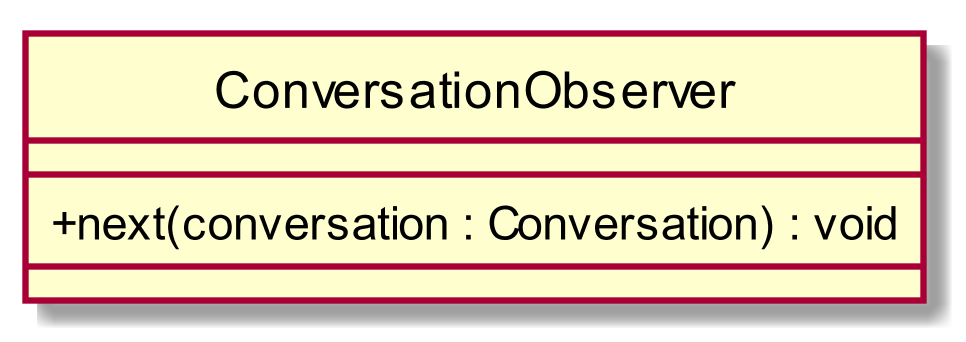
\includegraphics[width=\textwidth,height=\textheight,keepaspectratio]{images/ClassConversationObserver.png}
	\caption{Back-end::ConversationObserver}
\end{figure}
\begin{itemize}
	\item \textbf{Nome}: \file{ConversationObserver};
	\item \textbf{Tipo}: \file{Class};
	\item \textbf{Descrizione}: classe che rappresenta un \file{Observer} che si aspetta dati di tipo \file{Conversation}. ;
	\item \textbf{Utilizzo}: implementa il metodo \file{next()} dell'interfaccia, in maniera tale che accetti dati di tipo \file{Conversation};
	\item \textbf{Metodi}:
	\begin{itemize}
		\item[] \file{+ next(conversation: Conversation): void} \\
		Metodo che permette agli \file{Observable} di notificare l'\file{Observer} con dati di tipo \file{Conversation}. Definisce inoltre le operazioni che l'\file{Observer} compierà all'arrivo di tali dati;\\
		Parametri:
		\begin{itemize}
			\item \file{conversation: Conversation} \\
			Parametro contenente la \file{Conversation} mandata dall'\file{Observable};
		\end{itemize}
	\end{itemize}
\end{itemize}

\hypertarget{ConversationsDAODynamoDB_label}{\paragraph{ConversationsDAODynamoDB}}
\begin{figure}[h]
	\centering
	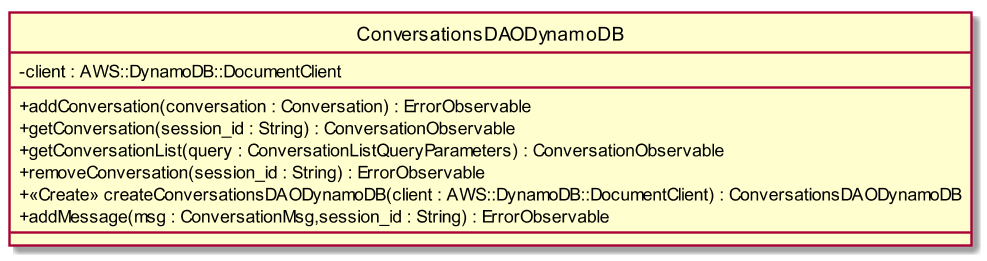
\includegraphics[width=\textwidth,height=\textheight,keepaspectratio]{images/ClassConversationsDAODynamoDB.png}
	\caption{Back-end::ConversationsDAODynamoDB}
\end{figure}
\begin{itemize}
	\item \textbf{Nome}: \file{ConversationsDAODynamoDB};
	\item \textbf{Tipo}: \file{Class};
	\item \textbf{Descrizione}: classe che si occupa di implementare l'interfaccia \file{ConversationsDAO}, utilizzando un database DynamoDB come supporto per la memorizzazione dei dati;
	\item \textbf{Utilizzo}: implementa i metodi dell'interfaccia \file{ConversationsDAO} interrogando un database DynamoDB. Utilizza \file{AWS::DynamoDB::DocumentClient} per l'accesso al database. La dependency injection dell'oggetto \file{AWS::DynamoDB} viene fatta utilizzando il costruttore;
	\item \textbf{Attributi}:
	\begin{itemize}
		\item[] \file{- db: AWS::DynamoDB} \\
		Attributo contenente un riferimento al modulo di Node.js utilizzato per l'accesso al database DynamoDB contenente la tabella degli utenti;
	\end{itemize}
	\item \textbf{Metodi}:
	\begin{itemize}
		\item[] \file{+ addConversation(conversation: Conversation): ErrorObservable} \\
		Implementazione del metodo definito nell'interfaccia \file{ConversationsDAO}. Utilizza il metodo put del \file{DocumentClient} per aggiungere la conversazione al database;\\
		Parametri:
		\begin{itemize}
			\item \file{conversation: Conversation} \\
			Parametro contenente la conversazione da inserire;
		\end{itemize}
		\item[] \file{+ getConversation(session\_id: String, timestamp: String): ConversationObservable} \\
		Implementazione del metodo definito nell'interfaccia \file{ConversationsDAO}. Utilizza il metodo get del \file{DocumentClient} per ottenere i dati relativi ad una \file{Conversation} dal database;\\
		Parametri:
		\begin{itemize}
			\item \file{session\_id: String} \\
			Parametro contenente l'id della sessione della conversazione da ricevere;
			\item \file{timestamp: String} \\
			Parametro contenente il timestamp relativo all'inizio della conversazione;
		\end{itemize}
		\item[] \file{+ getConversationList(): ConversationObservable} \\
		Implementazione del metodo dell'interfaccia \file{ConversationsDAO}. Utilizza il metodo scan del \file{DocumentClient} per ottenere la lista delle conversazioni dal database;\\
		\item[] \file{+ removeConversation(session\_id: String, timestamp: String): ErrorObservable} \\
		Implementazione del metodo dell'interfaccia \file{ConversationsDAO}. Utilizza il metodo delete del \file{DocumentClient} per eliminare una conversazione dal database;\\
		Parametri:
		\begin{itemize}
			\item \file{session\_id: String} \\
			Parametro contenente l'id della sessione della conversazione da eliminare;
			\item \file{timestamp: String} \\
			Parametro contenente il timestamp relativo all'inizio della conversazione;
		\end{itemize}
		\item[] \file{+ <> createConversationsDAODynamoDB(guest\_id: String, db: AWS::DynamoDB): ConversationsDAODynamoDB} \\
		Constructor della classe \file{ConversationsDAODynamoDB}. Permette di effettuare la dependency injection di \file{AWS::DynamoDB};\\
		Parametri:
		\begin{itemize}
			\item \file{guest\_id: String} \\
			sdadnoadnaosd;
			\item \file{db: AWS::DynamoDB} \\
			Parametro contenente un riferimento al modulo di Node.js da utilizzare per l'accesso al database DynamoDB contenente la tabella delle conversazioni;
		\end{itemize}
		\item[] \file{+ addMessage(msg: ConversationMsg, timestamp: String, session\_id: String): ErrorObservable} \\
		Implementazione del metodo definito nell'interfaccia \file{ConversationsDAO}. Utilizza il metodo put del \file{DocumentClient} per aggiungere un messaggio ad una conversazione;\\
		Parametri:
		\begin{itemize}
			\item \file{msg: ConversationMsg} \\
			Parametro contenente il messaggio.
;
			\item \file{timestamp: String} \\
			Parametro contenente il timestamp relativo all'inizio della conversazione;
			\item \file{session\_id: String} \\
			Parametro contenente l'id della sessione della conversazione dove aggiungere il messaggio;
		\end{itemize}
	\end{itemize}
\end{itemize}

\hypertarget{ConversationWebhookService_label}{\paragraph{ConversationWebhookService}}
\begin{figure}[h]
	\centering
	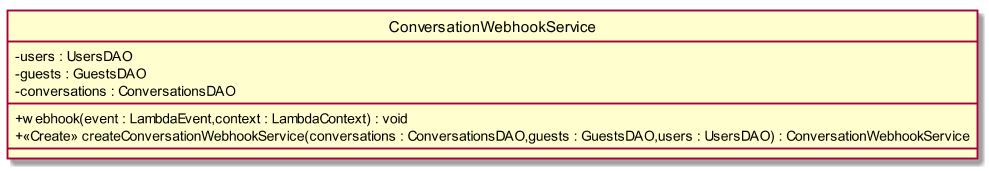
\includegraphics[width=\textwidth,height=\textheight,keepaspectratio]{images/ClassConversationWebhookService.png}
	\caption{Back-end::ConversationWebhookService}
\end{figure}
\begin{itemize}
	\item \textbf{Nome}: \file{ConversationWebhookService};
	\item \textbf{Tipo}: \file{Class};
	\item \textbf{Descrizione}: questa classe si occupa di implementare l'interfaccia \file{WebhookService}, implementando un Webhook che fornisce una risposta ad api.ai;
	\item \textbf{Utilizzo}: fornisce il metodo che si occupa di rispondere alle chiamate al microservizio da parte di api.ai;
	\item \textbf{Padre}: \file{<<interface>> WebhookService};
	\item \textbf{Attributi}:
	\begin{itemize}
		\item[] \file{- users: UsersDAO} \\
		Attributo che permette di contattare UsersDAO, il quale fornisce i meccanismi di accesso al database contenente gli utenti registrati;
		\item[] \file{- guests: GuestsDAO} \\
		Attributo che permette di contattare GuestDAO, il quale fornisce i meccanismi di accesso al database contenente gli ospiti;
		\item[] \file{- conversation: ConversationsDAO} \\
		Attributo che permette di contattare ConversationDAO, il quale fornisce i meccanismi di accesso al database delle conversazioni;
	\end{itemize}
	\item \textbf{Metodi}:
	\begin{itemize}
		\item[] \file{+ webhook(event: LambaEvent, context: LambdaContext): void} \\
		Questo metodo soddisfa i requisiti per webhook descritti da api.ai. Si occupa di cercare nei database la presenza di interazioni passate con la persona con cui sta avvenendo l'interazione, e di verificare se la persona in questione può essere un amministratore del sistema. Nel caso di interazioni passate il context accoglienza viene riempito con azienda e dati della persona con cui l'ospite ha avuto il maggior numero di incontri in passato, e viene chiesto di confermare se la persona indicata è quella a cui l'ospite è effettivamente interessato. Nel caso di amministratore viene impostato il context admin, in modo che api.ai riconosca l'utente come un potenziale amministratore e gli chieda se vuole entrare nell'area di amministrazione;\\
		Parametri:
		\begin{itemize}
			\item \file{event: LambaEvent} \\
			Parametro contenente, all'interno del campo \file{body} sotto forma di stringa in formato JSON, un oggetto contenente tutti i dati relativi ad una richiesta di api.ai al \file{ConversationWebhookService}. Tali dati sono:
\begin{lstlisting}[language=json,firstnumber=1]
{
  "id":"String",
  "lang":"String",
  "originalRequest":"Object",
  "result":"ProcessingResult",
  "sessionId":"String",
  "status":"StatusObject",
  "timestamp":"String"
 }
\end{lstlisting}
Per la relativa documentazione, consultare la pagina \url{https://docs.api.ai/docs/query#response};
			\item \file{context: LambdaContext} \\
			Parametro utilizzato dal webhook per inviare la risposta. La risposta, contenuta nel \file{LambdaResponse} parametro del metodo \file{LambdaContext::succeed}, possiede un attributo \file{body}, il quale conterrà il corpo di essa sotto forma di una stringa in formato JSON. \\
La risposta può essere una tra i seguenti tipi:
\begin{itemize}
    \item l'utente viene riconosciuto come un potenziale amministratore;
    \item l'utente viene riconosciuto come un ospite conosciuto.
\end{itemize}
Nel primo caso, la risposta fornita sarà così organizzata:
\begin{lstlisting}[language=json,firstnumber=1]
{
    "contexts": [{
        "name":"String",
        "first\_name":"String",
        "last\_name":"String",
        "username":"String"
    }]
}
\end{lstlisting}
Dove
\begin{itemize}
    \item \file{name} indica il nome del context, che in questo caso sarà "admin";
    \item \file{first\_name} indica il nome dell'amministratore;
    \item \file{last\_name} indica il cognome dell'amministratore;
    \item \file{username} indica lo username dell'amministratore;
\end{itemize}
Nel secondo caso, la risposta sarà così organizzata:
\begin{lstlisting}[language=json,firstnumber=1]
{
    "contexts": [{
        "name":"String",
        "name\_guest":"String",
        "company":"String",
        "first\_name":"String",
        "last\_name":"String"
    }]
}
\end{lstlisting}
Dove
\begin{itemize}
    \item \file{name} indica il nome del context, che in questo caso sarà "welcome";
    \item \file{name\_guest} indica il nome dell'ospite;
    \item \file{company} indica l'azienda di provenienza dell'ospite;
    \item \file{username} indica lo username dell'amministratore;
    \item \file{first\_name} indica il nome della persona desiderata;
    \item \file{last\_name} indica il cognome della persona desiderata;
\end{itemize};
		\end{itemize}
		\item[] \file{+ <<Create>> createConversationWebhookService(conversation: ConversationsDAO, guest: GuestsDAO, user: UsersDAO): ConversationWebhookService} \\
		Metodo che permette la costruzione di un \file{ConversationWebhookService}. Permette la dependency injection che ha come oggetti un \file{ConversationsDAO}, \file{GuestsDAO} e \file{UsersDAO};\\
		Parametri:
		\begin{itemize}
			\item \file{conversation: ConversationsDAO} \\
			Attributo contenente il  \file{ConversationsDAO};
			\item \file{guest: GuestsDAO} \\
			Attributo contenente il \file{GuestsDAO};
			\item \file{user: UsersDAO} \\
			Attributo contenente lo \file{UsersDAO};
		\end{itemize}
	\end{itemize}
\end{itemize}

\hypertarget{ErrorObservable_label}{\paragraph{ErrorObservable}}
\begin{figure}[h]
	\centering
	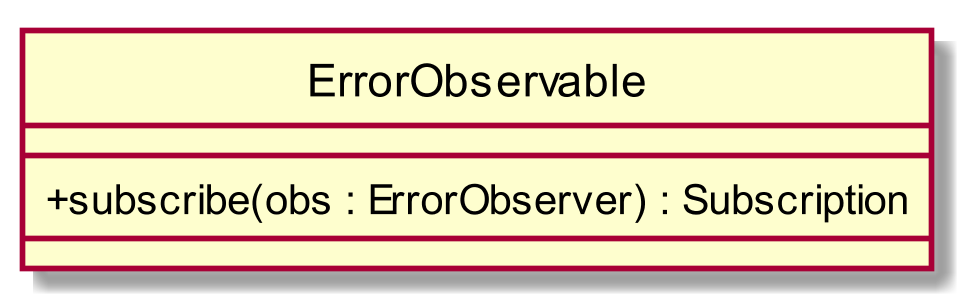
\includegraphics[width=\textwidth,height=\textheight,keepaspectratio]{images/ClassErrorObservable.png}
	\caption{Back-end::ErrorObservable}
\end{figure}
\begin{itemize}
	\item \textbf{Nome}: \file{ErrorObservable};
	\item \textbf{Tipo}: \file{Class};
	\item \textbf{Descrizione}: ????;
	\item \textbf{Utilizzo}: ????;
	\item \textbf{Padre}: \file{Observable};
\end{itemize}

\hypertarget{ErrorObserver_label}{\paragraph{ErrorObserver}}
\begin{figure}[h]
	\centering
	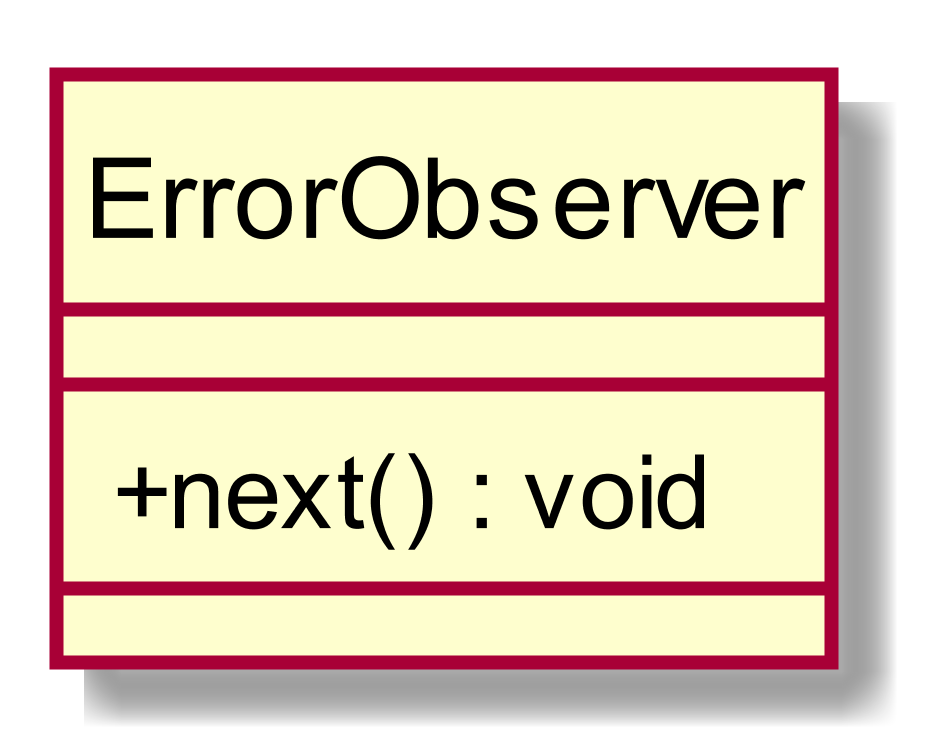
\includegraphics[width=\textwidth,height=\textheight,keepaspectratio]{images/ClassErrorObserver.png}
	\caption{Back-end::ErrorObserver}
\end{figure}
\begin{itemize}
	\item \textbf{Nome}: \file{ErrorObserver};
	\item \textbf{Tipo}: \file{Class};
	\item \textbf{Descrizione}: ????;
	\item \textbf{Utilizzo}: ????;
\end{itemize}

\hypertarget{Guest_label}{\paragraph{Guest}}
\begin{figure}[h]
	\centering
	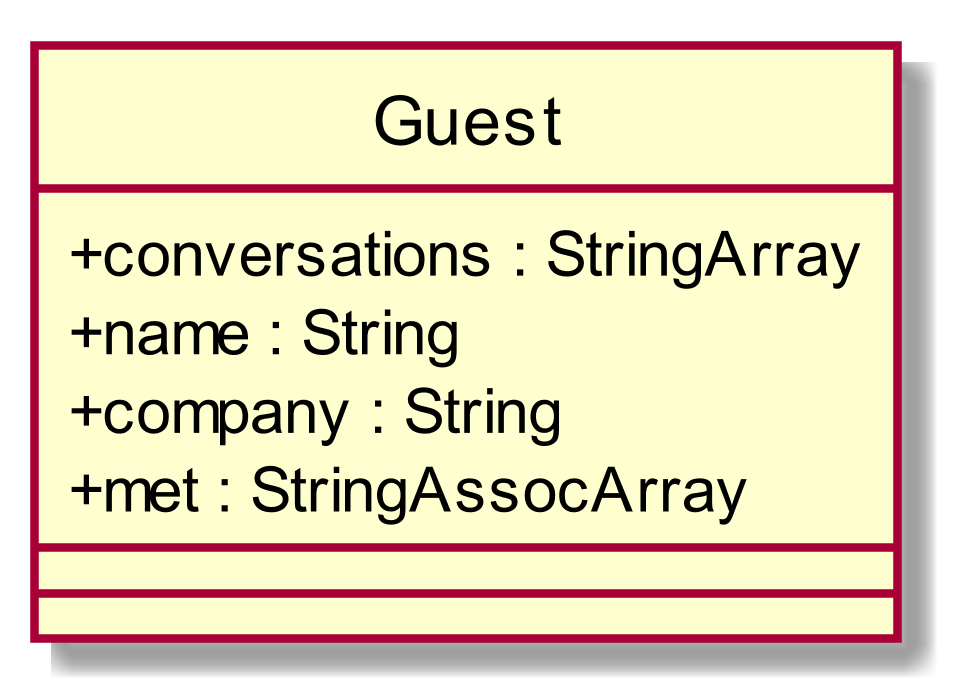
\includegraphics[width=\textwidth,height=\textheight,keepaspectratio]{images/ClassGuest.png}
	\caption{Back-end::Guest}
\end{figure}
\begin{itemize}
	\item \textbf{Nome}: \file{Guest};
	\item \textbf{Tipo}: \file{Class};
	\item \textbf{Descrizione}: questa classe si occupa di rappresentare e organizzare gli attributi relativi ad un ospite conosciuto, i quali dovranno essere salvati nel database;
	\item \textbf{Utilizzo}: fornisce gli attributi relativi ad un ospite;
	\item \textbf{Attributi}:
	\begin{itemize}
		\item[] \file{+ conversations: ConversationIdArray} \\
		Attributo contenente l'array delle conversazioni avute con l'ospite;
		\item[] \file{+ name: String} \\
		Attributo contenente il nome dell'ospite;
		\item[] \file{+ company: String} \\
		Attributo contenente l'azienda di provenienza dell'ospite;
		\item[] \file{+ met: StringAssocArray} \\
		Attributo contenente l'array associativo del numero di volte che una persona è stata accolta. La chiave di questo array associativo è il nome dell'ospite;
	\end{itemize}
\end{itemize}

\hypertarget{GuestObservable_label}{\paragraph{GuestObservable}}
\begin{figure}[h]
	\centering
	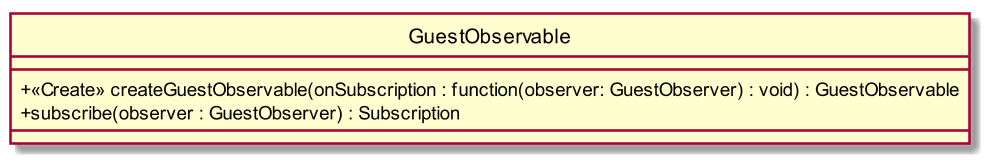
\includegraphics[width=\textwidth,height=\textheight,keepaspectratio]{images/ClassGuestObservable.png}
	\caption{Back-end::GuestObservable}
\end{figure}
\begin{itemize}
	\item \textbf{Nome}: \file{GuestObservable};
	\item \textbf{Tipo}: \file{Class};
	\item \textbf{Descrizione}: questa classe implementa un \file{Observable} che permette l'iscrizione di \file{GuestObserver};
	\item \textbf{Utilizzo}: fornisce i meccanismi necessari per il passaggio di una serie di \file{Guest} ad un \file{Observer} interessato;
	\item \textbf{Padre}: \file{Observable};
	\item \textbf{Metodi}:
	\begin{itemize}
		\item[] \file{+ <<Create>> createGuestObservable(onSubscription: function(observer: GuestObserver) : void): GuestObservable} \\
		Constructor di \file{GuestObservable};\\
		Parametri:
		\begin{itemize}
			\item \file{onSubscription: function(observer: GuestObserver) : void} \\
			Funzione che verrà eseguita quando un \file{Observer} si iscrive all'\file{Observable}. Si occupa di passare i dati all'\file{Observer}, chiamando il metodo \file{next(guest: Guest)}. Quando non ci sono più dati da restituire, si occupa di chiamare il metodo \file{complete()}. Nel caso in cui si verificasse un errore, si occupa di chiamare il metodo \file{error(err: Object)} con i dati relativi all'errore verificatosi;
		\end{itemize}
		\item[] \file{+ subscribe(observer: GuestObserver): Subscription} \\
		Metodo che permette ad un \file{GuestObserver} interessato di iscriversi a questo \file{Observable};\\
		Parametri:
		\begin{itemize}
			\item \file{observer: GuestObserver} \\
			\file{Observer} che si vuole iscrivere;
		\end{itemize}
	\end{itemize}
\end{itemize}

\hypertarget{GuestObserver_label}{\paragraph{GuestObserver}}
\begin{figure}[h]
	\centering
	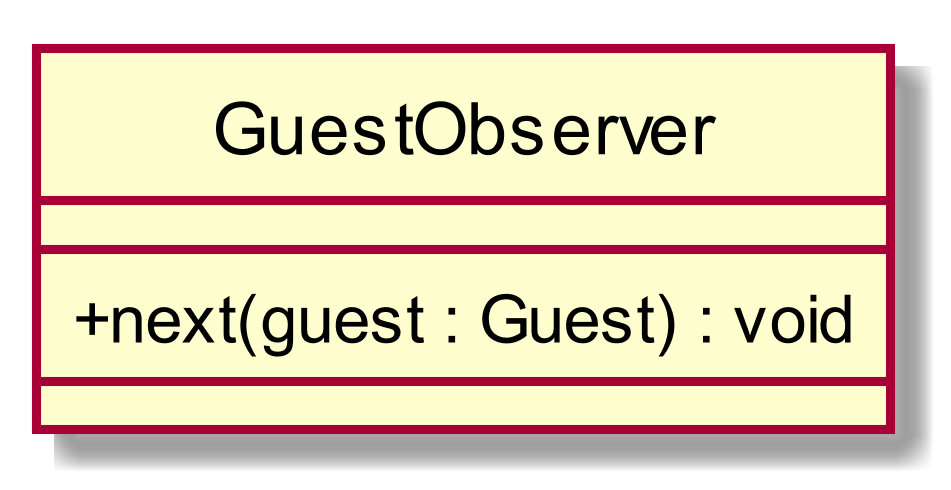
\includegraphics[width=\textwidth,height=\textheight,keepaspectratio]{images/ClassGuestObserver.png}
	\caption{Back-end::GuestObserver}
\end{figure}
\begin{itemize}
	\item \textbf{Nome}: \file{GuestObserver};
	\item \textbf{Tipo}: \file{Class};
	\item \textbf{Descrizione}: classe che rappresenta un \file{Observer} che si aspetta dati di tipo \file{Guest};
	\item \textbf{Utilizzo}: implementa il metodo \file{next()} dell'interfaccia, in maniera tale che accetti dati di tipo \file{Guest};
	\item \textbf{Metodi}:
	\begin{itemize}
		\item[] \file{+ next(guest: Guest): void} \\
		Metodo che permette agli \file{Observable} di notificare l'\file{Observer} con dati di tipo \file{Guest}. Definisce inoltre le operazioni che l'\file{Observer} compierà all'arrivo di tali dati;\\
		Parametri:
		\begin{itemize}
			\item \file{guest: Guest} \\
			Parametro contenente il \file{Guest} mandato dall'\file{Observable};
		\end{itemize}
	\end{itemize}
\end{itemize}

\hypertarget{GuestsDAODynamoDB_label}{\paragraph{GuestsDAODynamoDB}}
\begin{figure}[h]
	\centering
	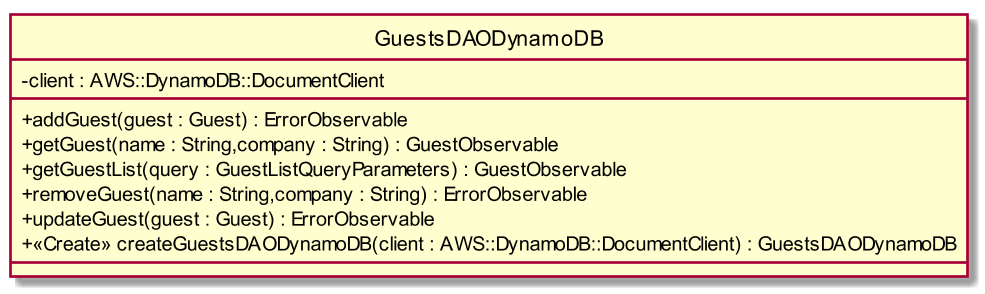
\includegraphics[width=\textwidth,height=\textheight,keepaspectratio]{images/ClassGuestsDAODynamoDB.png}
	\caption{Back-end::GuestsDAODynamoDB}
\end{figure}
\begin{itemize}
	\item \textbf{Nome}: \file{GuestsDAODynamoDB};
	\item \textbf{Tipo}: \file{Class};
	\item \textbf{Descrizione}: classe che si occupa di implementare l'interfaccia \file{GuestsDAO}, utilizzando un database DynamoDB come supporto per la memorizzazione dei dati;
	\item \textbf{Utilizzo}: implementa i metodi dell'interfaccia \file{GuestsDAO} interrogando un database DynamoDB. Utilizza \file{AWS::DynamoDB::DocumentClient} per l'accesso al database. La dependency injection dell'oggetto \file{AWS::DynamoDB} viene fatta utilizzando il costruttore;
	\item \textbf{Attributi}:
	\begin{itemize}
		\item[] \file{- db: AWS::DynamoDB} \\
		Attributo contenente un riferimento al modulo di Node.js utilizzato per l'accesso al database DynamoDB contenente la tabella degli utenti;
	\end{itemize}
	\item \textbf{Metodi}:
	\begin{itemize}
		\item[] \file{+ addGuest(guest: Guest): ErrorObservable} \\
		Implementazione del metodo definito nell'interfaccia \file{GuestsDAO}. Utilizza il metodo put del \file{DocumentClient} per aggiungere l'ospite al database;\\
		Parametri:
		\begin{itemize}
			\item \file{guest: Guest} \\
			Parametro contenente l'ospite da aggiungere;
		\end{itemize}
		\item[] \file{+ getGuest(name: String, company: String): GuestObservable} \\
		Implementazione del metodo definito nell'interfaccia \file{GuestsDAO}. Utilizza il metodo get del \file{DocumentClient} per ottenere i dati relativi ad un \file{Guest} dal database;\\
		Parametri:
		\begin{itemize}
			\item \file{name: String} \\
			Parametro contenente il nome dell'ospite;
			\item \file{company: String} \\
			Parametro contenente l'azienda di provenienza dell'ospite;
		\end{itemize}
		\item[] \file{+ getGuestList(): GuestObservable} \\
		Implementazione del metodo dell'interfaccia \file{GuestsDAO}. Utilizza il metodo scan del \file{DocumentClient} per ottenere la lista degli ospiti dal database;\\
		\item[] \file{+ removeGuest(name: String, company: String): ErrorObservable} \\
		Implementazione del metodo dell'interfaccia \file{GuestsDAO}. Utilizza il metodo delete del \file{DocumentClient} per eliminare un ospite dal database;\\
		Parametri:
		\begin{itemize}
			\item \file{name: String} \\
			Parametro contenente il nome dell'ospite;
			\item \file{company: String} \\
			Parametro contenente l'azienda di provenienza dell'ospite;
		\end{itemize}
		\item[] \file{+ updateGuest(guest: Guest): ErrorObservable} \\
		Implementazione del metodo dell'interfaccia \file{GuestsDAO}. Utilizza il metodo update del \file{DocumentClient} per aggiornare i dati relativi ad un ospite presenti all'interno del database;\\
		Parametri:
		\begin{itemize}
			\item \file{guest: Guest} \\
			Parametro contenente l'ospite da aggiornare;
		\end{itemize}
		\item[] \file{+ <> createGuestsDAODynamoDB(db: AWS::DynamoDB): GuestsDAODynamoDB} \\
		Constructor della classe \file{GuestsDAODynamoDB}. Permette di effettuare la dependency injection di \file{AWS::DynamoDB};\\
		Parametri:
		\begin{itemize}
			\item \file{db: AWS::DynamoDB} \\
			Parametro contenente un riferimento al modulo di Node.js da utilizzare per l'accesso al database DynamoDB contenente la tabella degli ospiti;
		\end{itemize}
	\end{itemize}
\end{itemize}

\hypertarget{RuleObservable_label}{\paragraph{RuleObservable}}
\begin{figure}[h]
	\centering
	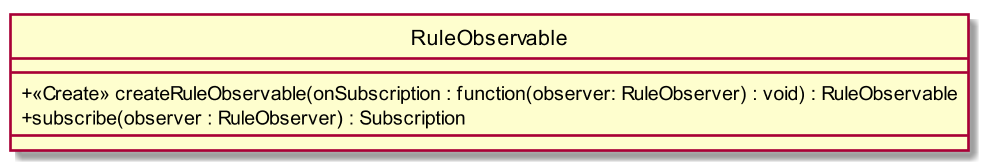
\includegraphics[width=\textwidth,height=\textheight,keepaspectratio]{images/ClassRuleObservable.png}
	\caption{Back-end::RuleObservable}
\end{figure}
\begin{itemize}
	\item \textbf{Nome}: \file{RuleObservable};
	\item \textbf{Tipo}: \file{Class};
	\item \textbf{Descrizione}: questa classe implementa un \file{Observable} che permette l'iscrizione di \file{RuleObserver};
	\item \textbf{Utilizzo}: fornisce i meccanismi necessari per il passaggio di una serie di \file{Rule} ad un \file{Observer} interessato;
	\item \textbf{Padre}: \file{Observable};
	\item \textbf{Metodi}:
	\begin{itemize}
		\item[] \file{+ <<Create>> createRuleObservable(onSubscription: function(observer: RuleObserver) : void): RuleObservable} \\
		Constructor di \file{RuleObservable};\\
		Parametri:
		\begin{itemize}
			\item \file{onSubscription: function(observer: RuleObserver) : void} \\
			Funzione che verrà eseguita quando un \file{Observer} si iscrive all'\file{Observable}. Si occupa di passare i dati all'\file{Observer}, chiamando il metodo \file{next(rule: Rule)}. Quando non ci sono più dati da restituire, si occupa di chiamare il metodo \file{complete()}. Nel caso in cui si verificasse un errore, si occupa di chiamare il metodo \file{error(err: Object)} con i dati relativi all'errore verificatosi;
		\end{itemize}
		\item[] \file{+ subscribe(observer: RuleObserver): Subscription} \\
		Metodo che permette ad un \file{RuleObserver} interessato di iscriversi a questo \file{Observable};\\
		Parametri:
		\begin{itemize}
			\item \file{observer: RuleObserver} \\
			\file{Observer} che si vuole iscrivere;
		\end{itemize}
	\end{itemize}
\end{itemize}

\hypertarget{RuleObserver_label}{\paragraph{RuleObserver}}
\begin{figure}[h]
	\centering
	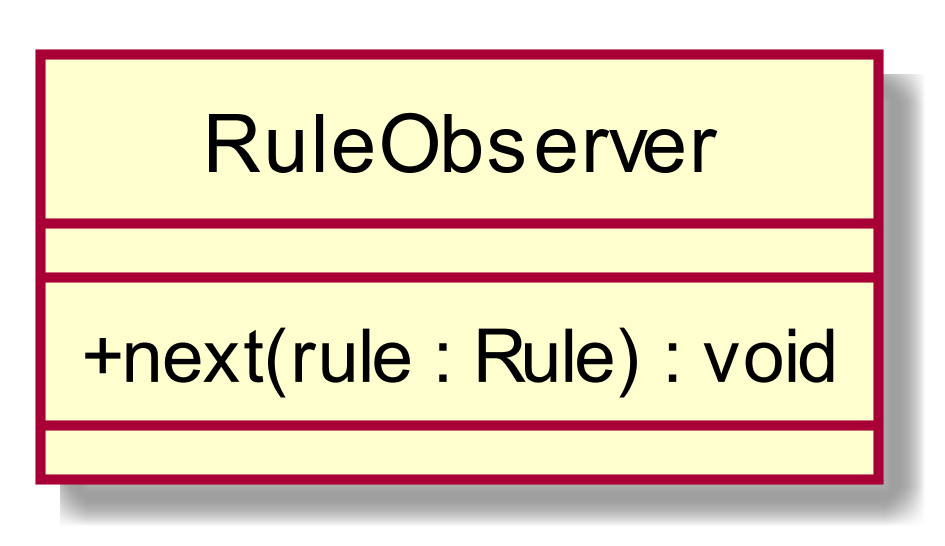
\includegraphics[width=\textwidth,height=\textheight,keepaspectratio]{images/ClassRuleObserver.png}
	\caption{Back-end::RuleObserver}
\end{figure}
\begin{itemize}
	\item \textbf{Nome}: \file{RuleObserver};
	\item \textbf{Tipo}: \file{Class};
	\item \textbf{Descrizione}: classe che rappresenta un \file{Observer} che si aspetta dati di tipo \file{Rule};
	\item \textbf{Utilizzo}: implementa il metodo \file{next()} dell'interfaccia, in maniera tale che accetti dati di tipo \file{Rule};
	\item \textbf{Metodi}:
	\begin{itemize}
		\item[] \file{+ next(rule: Rule): void} \\
		Metodo che permette agli \file{Observable} di notificare l'\file{Observer} con dati di tipo \file{Rule}. Definisce inoltre le operazioni che l'\file{Observer} compierà all'arrivo di tali dati;\\
		Parametri:
		\begin{itemize}
			\item \file{rule: Rule} \\
			Parametro contenente la \file{Rule} mandata dall'\file{Observable};
		\end{itemize}
	\end{itemize}
\end{itemize}

\hypertarget{SNSEvent_label}{\paragraph{SNSEvent}}
\begin{figure}[h]
	\centering
	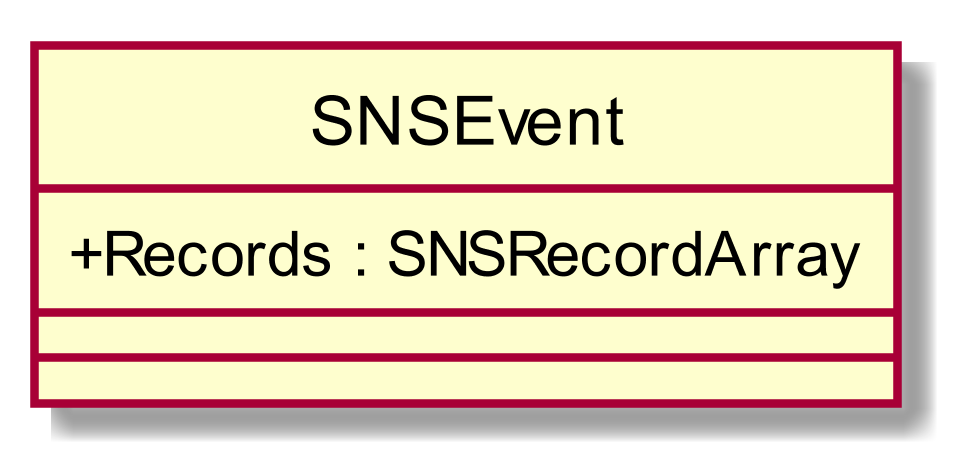
\includegraphics[width=\textwidth,height=\textheight,keepaspectratio]{images/ClassSNSEvent.png}
	\caption{Back-end::SNSEvent}
\end{figure}
\begin{itemize}
	\item \textbf{Nome}: \file{SNSEvent};
	\item \textbf{Tipo}: \file{Class};
	\item \textbf{Descrizione}: questa classe rappresentaa l'oggetto ricevuto da una lambda function in seguito alla pubblicazione di un messaggio su un topic di SNS a cui tale funzione è iscritta;
	\item \textbf{Utilizzo}: fornisce gli attributi relativi ad una notifica mandata da SNS ad una lambda function iscritta ad un topic sul quale sia stato pubblicato un messaggio;
	\item \textbf{Attributi}:
	\begin{itemize}
		\item[] \file{+ Records: SNSRecordArray} \\
		Array contenente i dati della notifica mandata da SNS alla lambda function. Contiene un unico oggetto di tipo Record;
	\end{itemize}
\end{itemize}

\hypertarget{SNSMessage_label}{\paragraph{SNSMessage}}
\begin{figure}[h]
	\centering
	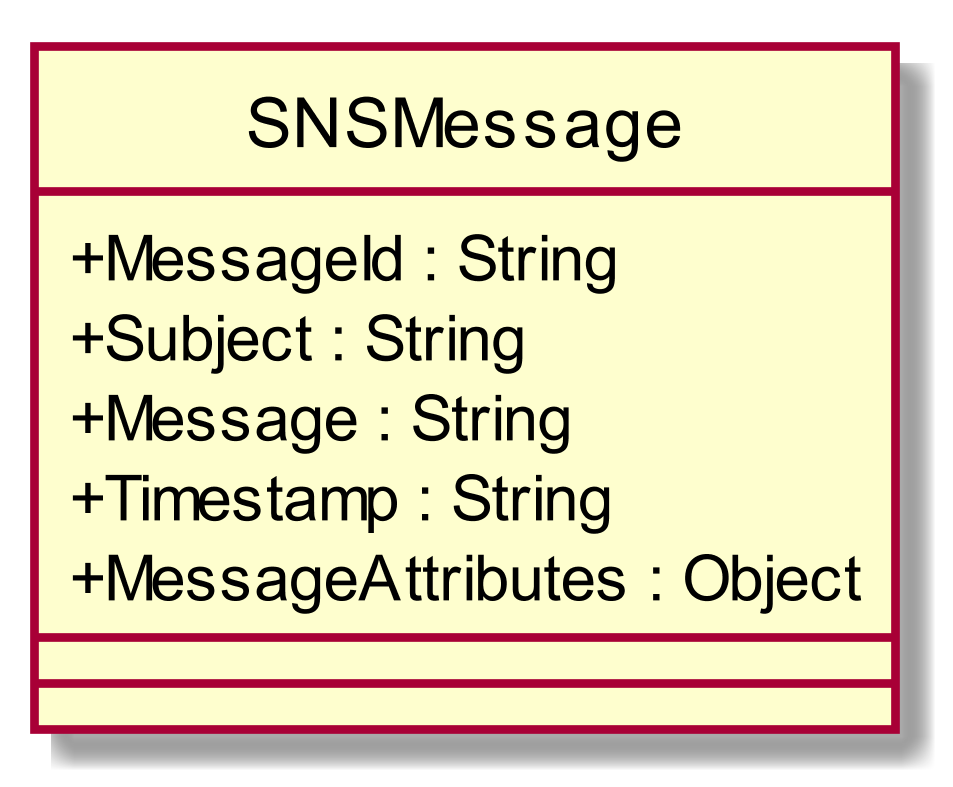
\includegraphics[width=\textwidth,height=\textheight,keepaspectratio]{images/ClassSNSMessage.png}
	\caption{Back-end::SNSMessage}
\end{figure}
\begin{itemize}
	\item \textbf{Nome}: \file{SNSMessage};
	\item \textbf{Tipo}: \file{Class};
	\item \textbf{Descrizione}: questa classe rappresenta un messaggio mandato da SNS in seguito ad un'interazione con l'assistente virtuale;
	\item \textbf{Utilizzo}: fornisce un meccanismo event-driven per la gestione dei dati relativi alle interazioni col sistema.\\
Per la relativa documentazione, consultare la pagina \url{http://docs.aws.amazon.com/sns/latest/dg/json-formats.html#http-subscription-confirmation-json};
	\item \textbf{Attributi}:
	\begin{itemize}
		\item[] \file{+ MessageId: String} \\
		Attributo contenente l'identificativo del messaggio;
		\item[] \file{+ Subject: String} \\
		Attributo contenente il Subject che dev'essere notificato dal sistema SNS;
		\item[] \file{+ Message: String} \\
		Attributo contenente il messaggio da pubblicare;
		\item[] \file{+ Timestamp: String} \\
		Attributo contenente il timestamp relativo al momento della pubblicazione del messaggio;
		\item[] \file{+ MessageAttributes: SnsMessageAttributes} \\
		Attributo contenente;
	\end{itemize}
\end{itemize}

\hypertarget{SNSRecord_label}{\paragraph{SNSRecord}}
\begin{figure}[h]
	\centering
	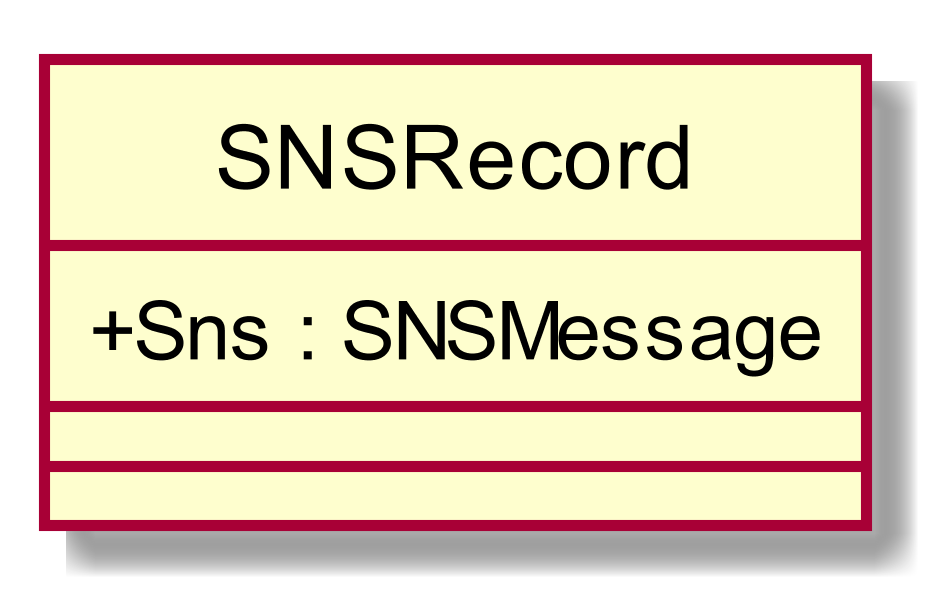
\includegraphics[width=\textwidth,height=\textheight,keepaspectratio]{images/ClassSNSRecord.png}
	\caption{Back-end::SNSRecord}
\end{figure}
\begin{itemize}
	\item \textbf{Nome}: \file{SNSRecord};
	\item \textbf{Tipo}: \file{Class};
	\item \textbf{Descrizione}: questa classe rappresenta uno dei records mandati da SNS ad una lambda function. ;
	\item \textbf{Utilizzo}: fornisce gli attributi di un record mandato da SNS ad una lambda function. ;
	\item \textbf{Attributi}:
	\begin{itemize}
		\item[] \file{+ Sns: SNSMessage} \\
		;
	\end{itemize}
\end{itemize}

\hypertarget{STTParams_label}{\paragraph{STTParams}}
\begin{figure}[h]
	\centering
	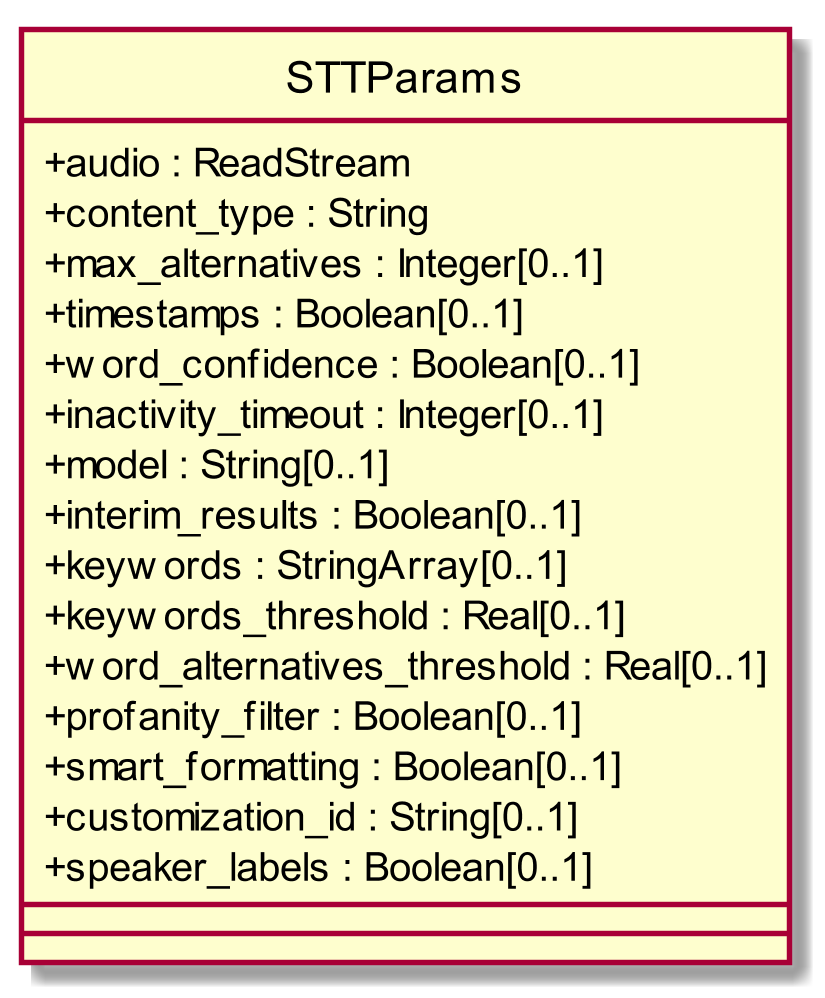
\includegraphics[width=\textwidth,height=\textheight,keepaspectratio]{images/ClassSTTParams.png}
	\caption{Back-end::STTParams}
\end{figure}
\begin{itemize}
	\item \textbf{Nome}: \file{STTParams};
	\item \textbf{Tipo}: \file{Class};
	\item \textbf{Descrizione}: questa classe si occupa di rappresentare ed organizzare i parametri necessari a richiamare le API Watson Speech to Text;
	\item \textbf{Utilizzo}: fornisce l'insieme dei parametri necessari ad identificare un audio, nel formato richiesto dall'API Watson Speech to Text, che verrà poi convertito in testo.
Per la relativa documentazione, consultare la pagina \url{https://www.ibm.com/watson/developercloud/speech-to-text/api/v1/#recognize_audio_websockets};
	\item \textbf{Attributi}:
	\begin{itemize}
		\item[] \file{+ audio: ReadStream} \\
		Attributo contenente lo stream per la lettura del file audio;
		\item[] \file{+ content\_type: String} \\
		Attributo contenente il formato dell'audio;
		\item[] \file{+ max\_alternatives: Integer[0..1]} \\
		Attributo contenente il numero massimo di alternative testuali che devono essere fornite per il relativo audio. Il valore di default di questo attributo è uguale a 1;
		\item[] \file{+ timestamps: Boolean[0..1]} \\
		Attributo contenente un valore booleano che indica se ottenere un timestamp per ogni parola. Il valore di default per questo attributo è false;
		\item[] \file{+ word\_confidence: Boolean[0..1]} \\
		Attributo contenente un valore booleano che indica se ottenere il grado di confidenza, contenuto nell'intervallo [0,1], per ogni parola. Il valore di default per questo attributo è false;
		\item[] \file{+ inactivity\_timeout: Integer[0..1]} \\
		Attributo contenente il tempo in secondi dopo il quale, se nell'audio viene rilevato solo del silenzio, la connessione deve essere chiusa. Il valore di default di questo attributo è 30 secondi. \\
Per non chiudere mai la connessione, si può impostare questo attributo a -1. ;
		\item[] \file{+ model: String[0..1]} \\
		Attributo contenente il nome del model relativo all'audio da trascrivere.\\
Un model è un parametro che indica la lingua e il tipo di sampling rates usato per essa.
Il tipo del sampling rates supportato può assumere uno tra i seguenti valori:
\begin{itemize}
\item broadband;
\item narrowband.
\end{itemize}
Si rimanda alla relativa documentazione (\url{https://www.ibm.com/watson/developercloud/speech-to-text/api/v1/?curl#get_models}) per ulteriori chiarimenti;
		\item[] \file{+ interim\_results: Boolean[0..1]} \\
		Attributo contenente un valore booleano che indica se posso essere ritornati risultati parziali o meno. Se impostato a true, i risultati parziali sono ritornati come uno stream di oggetti JSON ed ognuno di essi rappresenta un singolo SpeechRecognitionEvent. Se impostato a false, verrà ritornato un unico SpeechRecognitionEvent contenente il risultato finale. \\
Questro attributo ha valore di default uguale a false;
		\item[] \file{+ keywords: StringArray[0..1]} \\
		Attributo contenente l'array delle parole da ricercare nell'audio. Ogni cella di questo array può contenere una o più parole da cercare.
;
		\item[] \file{+ keywords\_threshold: Real[0..1]} \\
		Attributo contenente un valore di confidenza, contenuto nell'intervallo [0,1], che è il limite inferiore per una keyword trovata. Una parola fa match in una keyword se la sua confidenza è maggiore o uguale al valore di questo attributo. \\
Se questo parametro è omesso, nessuna keyword sarà trovata, altrimenti deve essere fornita almeno una keyword;
		\item[] \file{+ word\_alternatives\_threshold: Real[0..1]} \\
		Attributo contenente un valore di confindenza, contenuto nell'intervallo [0,1], che è il limite inferiore per identificare un'ipotetica parola come possibile alternativa. \\
Una parola alternativa è considerata tale se la sua confidenza è maggiore o uguale al valore di questo attributo. Se questo parametro è omesso, nessuna parola alternativa verrà fornita;
		\item[] \file{+ profanity\_filter: Boolean[0..1]} \\
		Attributo contenente un valore booleano che indica se il profanity filter verrà applicato al testo trascritto. \\
Il profanity filter è un meccanismo che sostituisce parole inappropriate con degli asterischi. Questo filtro può essere applicato solo a trascrizioni in lingua US English. \\
Il valore di default per questo attributo è uguale a true;
		\item[] \file{+ smart\_formatting: Boolean[0..1]} \\
		Attributo contenente un valore booleano che indica se date, orari, serie di numeri e cifre, numeri di telefono, valori monetari e indirizzi Internet devono essere convertiti, nella trascrizione finale, in un formato più leggibile. Questo meccanismo può essere applicato solo a trascrizioni in lingua US English. \\
Il valore di default per questo attributo è uguale a false;
		\item[] \file{+ customization\_id: String[0..1]} \\
		Attributo contenente il GUID relativo al model personalizzato utilizzato. Per default, nessun modello personalizzato è utilizzato;
		\item[] \file{+ speaker\_labels: Boolean[0..1]} \\
		Indicates whether labels that identify which words were spoken by which participants in a multi-person exchange are to be included in the response. If true, speaker labels are returned; if false (the default), they are not. Speaker labels can be returned only for the following language models:
en-US\_NarrowbandModel
es-ES\_NarrowbandModel
ja-JP\_NarrowbandModel
Setting speaker\_labels to true forces the continuous and timestamps parameters to be true, as well, regardless of whether the user specifies false for the parameters. For more information, see Speaker labels;
	\end{itemize}
\end{itemize}

\hypertarget{TaskObservable_label}{\paragraph{TaskObservable}}
\begin{figure}[h]
	\centering
	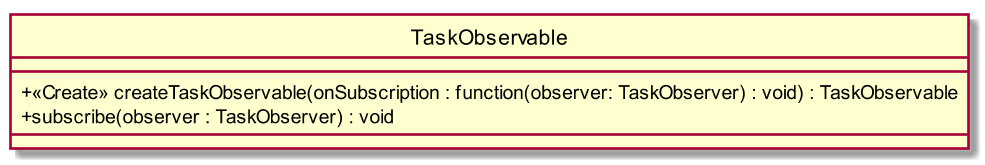
\includegraphics[width=\textwidth,height=\textheight,keepaspectratio]{images/ClassTaskObservable.png}
	\caption{Back-end::TaskObservable}
\end{figure}
\begin{itemize}
	\item \textbf{Nome}: \file{TaskObservable};
	\item \textbf{Tipo}: \file{Class};
	\item \textbf{Descrizione}: questa classe implementa un \file{Observable} che permette l'iscrizione di \file{TaskObserver};
	\item \textbf{Utilizzo}: fornisce i meccanismi necessari per il passaggio di una serie di \file{Task} ad un \file{Observer} interessato;
	\item \textbf{Padre}: \file{Observable};
	\item \textbf{Metodi}:
	\begin{itemize}
		\item[] \file{+ <<Create>> createTaskObservable(onSubscription: function(observer: TaskObserver) : void): TaskObservable} \\
		Constructor di \file{TaskObservable};\\
		Parametri:
		\begin{itemize}
			\item \file{onSubscription: function(observer: TaskObserver) : void} \\
			Funzione che verrà eseguita quando un \file{Observer} si iscrive all'\file{Observable}. Si occupa di passare i dati all'\file{Observer}, chiamando il metodo \file{next(function: Task)}. Quando non ci sono più dati da restituire, si occupa di chiamare il metodo \file{complete()}. Nel caso in cui si verificasse un errore, si occupa di chiamare il metodo \file{error(err: Object)} con i dati relativi all'errore verificatosi;
		\end{itemize}
		\item[] \file{+ subscribe(observer: TaskObserver): void} \\
		Metodo che permette ad un \file{TaskObserver} interessato di iscriversi a questo \file{Observable};\\
		Parametri:
		\begin{itemize}
			\item \file{observer: TaskObserver} \\
			\file{Observer} che si vuole iscrivere;
		\end{itemize}
	\end{itemize}
\end{itemize}

\hypertarget{TaskObserver_label}{\paragraph{TaskObserver}}
\begin{figure}[h]
	\centering
	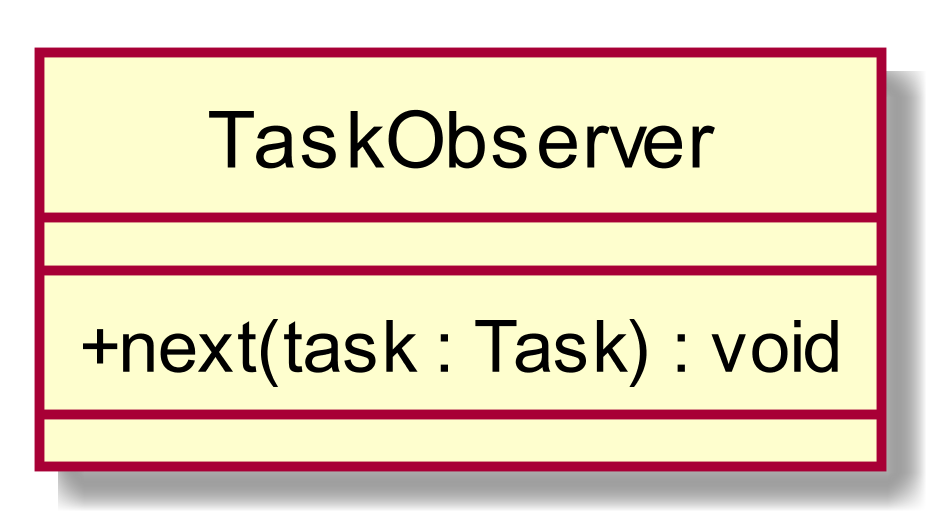
\includegraphics[width=\textwidth,height=\textheight,keepaspectratio]{images/ClassTaskObserver.png}
	\caption{Back-end::TaskObserver}
\end{figure}
\begin{itemize}
	\item \textbf{Nome}: \file{TaskObserver};
	\item \textbf{Tipo}: \file{Class};
	\item \textbf{Descrizione}: classe che rappresenta un \file{Observer} che si aspetta dati di tipo \file{Task};
	\item \textbf{Utilizzo}: implementa il metodo \file{next()} dell'interfaccia, in maniera tale che accetti dati di tipo \file{Task};
	\item \textbf{Metodi}:
	\begin{itemize}
		\item[] \file{+ next(task: Task): void} \\
		Metodo che permette agli \file{Observable} di notificare l'\file{Observer} con dati di tipo \file{Task}. Definisce inoltre le operazioni che l'\file{Observer} compierà all'arrivo di tali dati;\\
		Parametri:
		\begin{itemize}
			\item \file{task: Task} \\
			Parametro contenente la \file{Task} mandata dall'\file{Observable};
		\end{itemize}
	\end{itemize}
\end{itemize}

\hypertarget{UserObservable_label}{\paragraph{UserObservable}}
\begin{figure}[h]
	\centering
	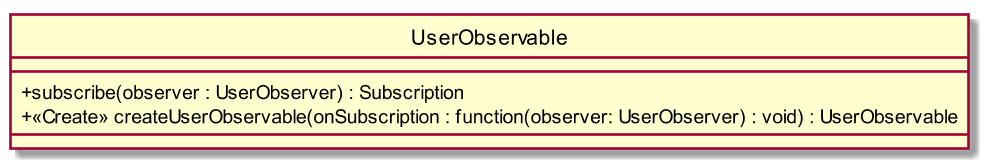
\includegraphics[width=\textwidth,height=\textheight,keepaspectratio]{images/ClassUserObservable.png}
	\caption{Back-end::UserObservable}
\end{figure}
\begin{itemize}
	\item \textbf{Nome}: \file{UserObservable};
	\item \textbf{Tipo}: \file{Class};
	\item \textbf{Descrizione}: questa classe implementa un \file{Observable} che permette l'iscrizione di \file{UserObserver};
	\item \textbf{Utilizzo}: fornisce i meccanismi necessari per il passaggio di una serie di \file{User} ad un \file{Observer} interessato;
	\item \textbf{Padre}: \file{Observable};
	\item \textbf{Metodi}:
	\begin{itemize}
		\item[] \file{+ subscribe(observer: UserObserver): Subscription} \\
		Metodo che permette ad uno \file{UserObserver} interessato di iscriversi a questo \file{Observable};\\
		Parametri:
		\begin{itemize}
			\item \file{observer: UserObserver} \\
			\file{Observer} che si vuole iscrivere;
		\end{itemize}
		\item[] \file{+ <<Create>> createUserObservable(onSubscription: function(observer: UserObserver) : void): UserObservable} \\
		Constructor di \file{UserObservable};\\
		Parametri:
		\begin{itemize}
			\item \file{onSubscription: function(observer: UserObserver) : void} \\
			Funzione che verrà eseguita quando un \file{Observer} si iscrive all'\file{Observable}. Si occupa di passare i dati all'\file{Observer}, chiamando il metodo \file{next(user: User)}. Quando non ci sono più dati da restituire, si occupa di chiamare il metodo \file{complete()}. Nel caso in cui si verificasse un errore, si occupa di chiamare il metodo \file{error(err: Object)} con i dati relativi all'errore verificatosi;
		\end{itemize}
	\end{itemize}
\end{itemize}

\hypertarget{UserObserver_label}{\paragraph{UserObserver}}
\begin{figure}[h]
	\centering
	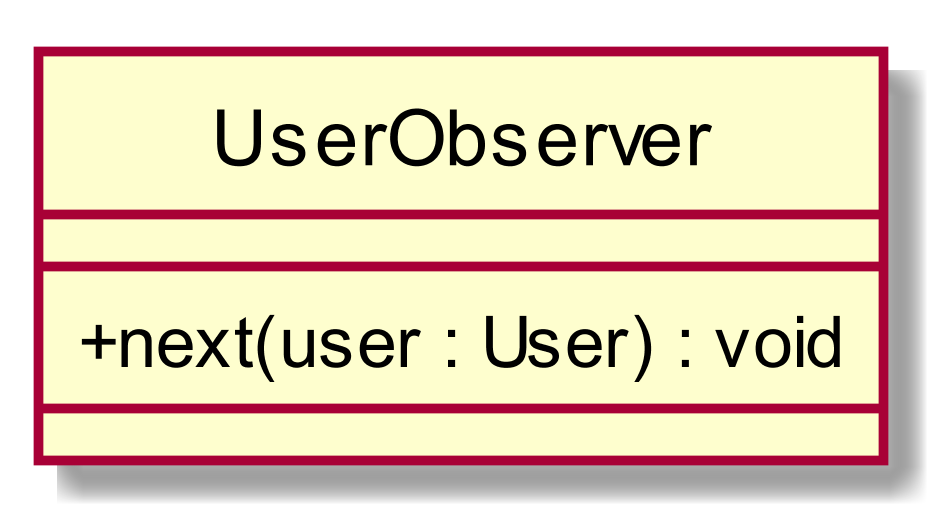
\includegraphics[width=\textwidth,height=\textheight,keepaspectratio]{images/ClassUserObserver.png}
	\caption{Back-end::UserObserver}
\end{figure}
\begin{itemize}
	\item \textbf{Nome}: \file{UserObserver};
	\item \textbf{Tipo}: \file{Class};
	\item \textbf{Descrizione}: classe che rappresenta un \file{Observer} che si aspetta dati di tipo \file{User}. ;
	\item \textbf{Utilizzo}: implementa il metodo \file{next()} dell'interfaccia, in maniera tale che accetti dati di tipo \file{User};
	\item \textbf{Metodi}:
	\begin{itemize}
		\item[] \file{+ next(user: User): void} \\
		Metodo che permette agli \file{Observable} di notificare l'\file{Observer} con dati di tipo \file{User}. Definisce inoltre le operazioni che l'\file{Observer} compierà all'arrivo di tali dati;\\
		Parametri:
		\begin{itemize}
			\item \file{user: User} \\
			Parametro contenente lo \file{User} mandato dall'\file{Observable};
		\end{itemize}
	\end{itemize}
\end{itemize}

\hypertarget{VAMessageListener_label}{\paragraph{VAMessageListener}}
\begin{figure}[h]
	\centering
	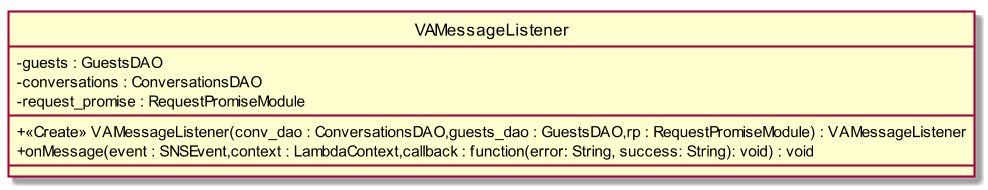
\includegraphics[width=\textwidth,height=\textheight,keepaspectratio]{images/ClassVAMessageListener.png}
	\caption{Back-end::VAMessageListener}
\end{figure}
\begin{itemize}
	\item \textbf{Nome}: \file{VAMessageListener};
	\item \textbf{Tipo}: \file{Class};
	\item \textbf{Descrizione}: questa classe si occupa di registrare i dati relativi alle interazioni degli ospiti col nostro sistema;
	\item \textbf{Utilizzo}: fornisce un meccanismo per registrare i dialoghi che gli ospiti hanno con il sitema. Fornisce una lambda function che quando viene generato un evento \file{SNSMessage} in seguito all'arrivo di una risposta da parte dell'assistente virtuale, si occupa di registrare i dati della relativa interazione tramite \file{ConvarsationsDAO}, ed eventualmente di aggiornare i dati relativi all'ospite utilizzando \file{GuestsDAO}. \\
SNS chiama tale lambda function con un oggetto del tipo \file{SNSEvent}, il quale contiene al suo interno un array di \file{SNSRecord}. Questo array in realtà ha un unico oggetto, il quale al suo interno contiene l'\file{SNSMessage} inviato. \\
Di seguito viene riportato un esempio dell'oggetto utilizzato.
\begin{lstlisting}[language=json,firstnumber=1]
{
  "Records":
  [
    {
      "Sns":
      {
        "Message": "Corpo del messaggio pubblicato sul topic di SNS",
        "MessageAttributes":{"key": "value", "key2": "value2"},
        "MessageId":"stringa-contenente-id-del-messaggio",
        "Subject":"oggetto del messaggio",
        "Timestamp":"2017-03-26T20:39:48.599Z"
      }
    }
  ]
}
\end{lstlisting};
	\item \textbf{Attributi}:
	\begin{itemize}
		\item[] \file{- guests: GuestsDAO} \\
		Attributo che permette di contattare il \file{GuestsDAO};
		\item[] \file{- conversations: ConversationDAO} \\
		Attributo che permette di contattare il \file{ConversationsDAO};
	\end{itemize}
	\item \textbf{Eventi gestiti}:
	\begin{itemize}
\item \file{SNSEvent} \\ Messaggio mandato ad sns quando arriva la risposta dall'assistente virtuale. All'arrivo del messaggio si occupa di salvare i dati dell'interazione nel DAO.	\end{itemize}
\end{itemize}

\subsection{Back-end::APIGateway}
Package contenente le componenti necessarie a gestire le richieste ricevute dal backend.
\subsubsection{Classi}
\hypertarget{Enrollment_label}{\paragraph{Enrollment}}
\begin{figure}[h]
	\centering
	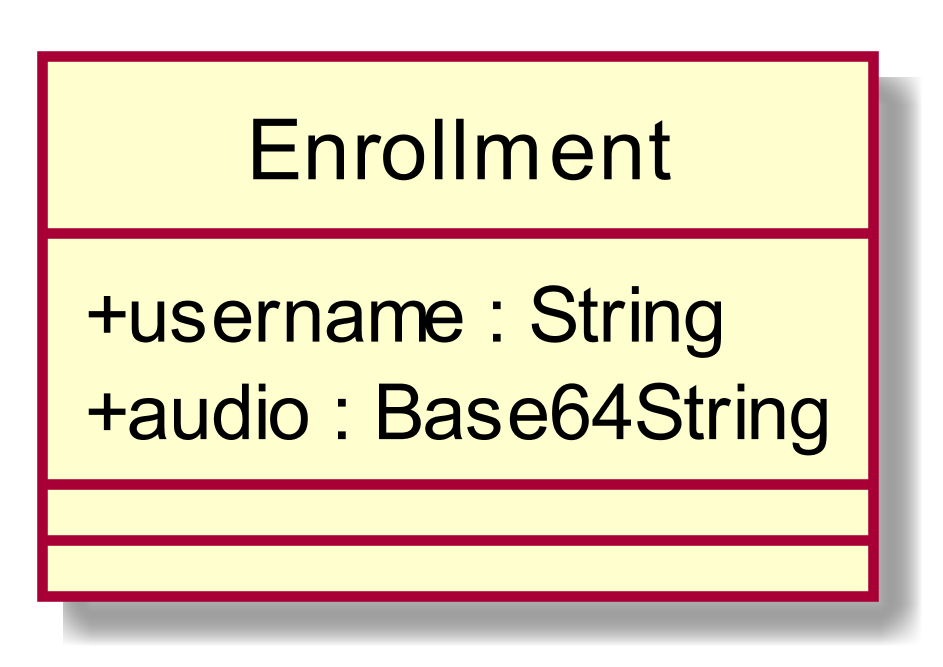
\includegraphics[width=\textwidth,height=\textheight,keepaspectratio]{images/ClassEnrollment.png}
	\caption{Back-end::APIGateway::Enrollment}
\end{figure}
\begin{itemize}
	\item \textbf{Nome}: \file{Enrollment};
	\item \textbf{Tipo}: \file{Class};
	\item \textbf{Descrizione}: questa classe fornisce gli attributi necessari al passaggio di un Enrollment alle lambda function;
	\item \textbf{Utilizzo}: fornisce gli attributi relativi ad un Enrollment;
	\item \textbf{Attributi}:
	\begin{itemize}
		\item[] \file{+ username: String} \\
		Attributo contenente l'username dell'utente associato all'Enrollment;
		\item[] \file{+ audio: Base64String} \\
		Attributo contenente la traccia audio che sarà oggetto dell'Enrollment, codificata in Base64;
	\end{itemize}
\end{itemize}

\hypertarget{VARequestAPIBody DA MODIFICARE DA MODIFICARE DA MODIFICARE DA MODIFICARE_label}{\paragraph{VARequestAPIBody DA MODIFICARE DA MODIFICARE DA MODIFICARE DA MODIFICARE}}
\begin{figure}[h]
	\centering
	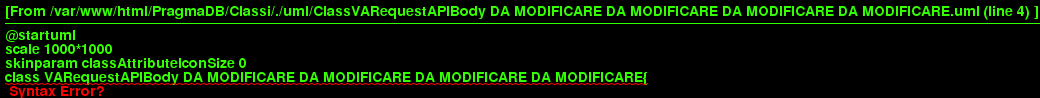
\includegraphics[width=\textwidth,height=\textheight,keepaspectratio]{images/ClassVARequestAPIBody DA MODIFICARE DA MODIFICARE DA MODIFICARE DA MODIFICARE.png}
	\caption{Back-end::APIGateway::VARequestAPIBody DA MODIFICARE DA MODIFICARE DA MODIFICARE DA MODIFICARE}
\end{figure}
\begin{itemize}
	\item \textbf{Nome}: \file{VARequestAPIBody DA MODIFICARE DA MODIFICARE DA MODIFICARE DA MODIFICARE};
	\item \textbf{Tipo}: \file{Class};
	\item \textbf{Descrizione}: questa classe fornisce gli attributi necessari al client per effettuare una richiesta all'API REST del back-end;
	\item \textbf{Utilizzo}: fornisce gli attributi relativi ad una richiesta all'API REST del back-end e viene utilizzata dalla classe \file{VARequestAPIEvent}. DA MODIFICARE DA MODIFICARE DA MODIFICARE DA MODIFICARE DA MODIFICARE DA MODIFICARE (manca la classe VARequestAPIEvent);
	\item \textbf{Attributi}:
	\begin{itemize}
		\item[] \file{+ app: String} \\
		Attributo contenente il nome dell'applicazione da cui arriva la richiesta;
		\item[] \file{+ session\_id: String} \\
		Attributo contenente l'id della sessione corrente, creato dal Client;
		\item[] \file{+ audio: Base64String} \\
		Attributo contenente l'audio della richiesta codificata in Base64;
		\item[] \file{+ data: ObjectAssocArray} \\
		Attributo contenente un array associativo di \file{Object} ricevuti dall'Assistente Virtuale;
	\end{itemize}
\end{itemize}

\hypertarget{VocalAPI_label}{\paragraph{VocalAPI}}
\begin{figure}[h]
	\centering
	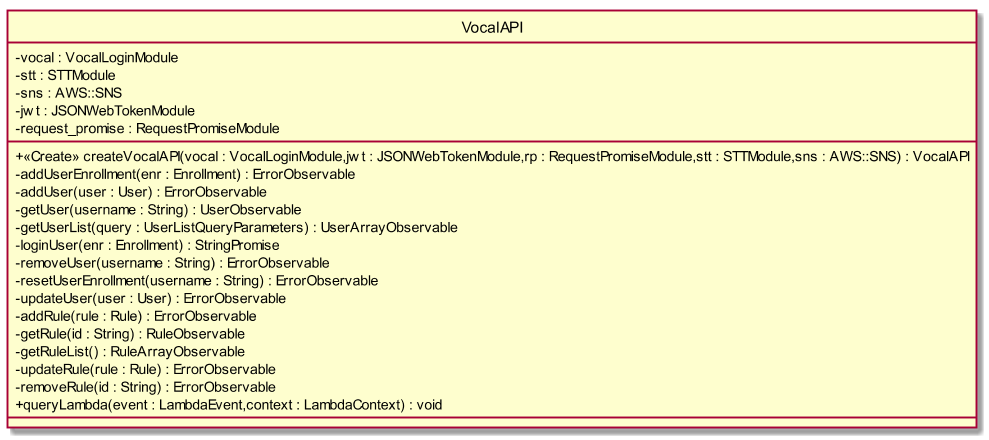
\includegraphics[width=\textwidth,height=\textheight,keepaspectratio]{images/ClassVocalAPI.png}
	\caption{Back-end::APIGateway::VocalAPI}
\end{figure}
\begin{itemize}
	\item \textbf{Nome}: \file{VocalAPI};
	\item \textbf{Tipo}: \file{Class};
	\item \textbf{Descrizione}: questa classe si occupa di implementare l'endpoint dell'API Gateway utilizzato dal client vocale;
	\item \textbf{Utilizzo}: grazie al metodo pubblico di questa classe, fornisce un meccanismo che:
\begin{itemize}
  \item permette di dedurre, tramite i microservizi di STT e di assistente virtuale, il servizio necessario al client vocale, utilizzando il metodo \file{queryLambda};
  \item permette al client vocale di usufruire delle funzionalità, supportate dal \file{Backend}, tramite i metodi privati che questa classe fornisce.
\end{itemize}
;
	\item \textbf{Attributi}:
	\begin{itemize}
		\item[] \file{- vocal: VocalLoginModule} \\
		Attributo contenente il \file{VocalLoginModule} di cui è stata eseguita la dependency injection nel costruttore. Viene utilizzato per effettuare il login nel servizio di Speaker Recognition;
		\item[] \file{- stt: STTModule} \\
		Attributo contenente il modulo utilizzato per contattare le API per il servizio di Watson Speech to Text di IBM;
		\item[] \file{- sns: AWS::SNS} \\
		Attributo che permette di contattare il servizio SNS;
		\item[] \file{- jwt: JSONWebTokenModule} \\
		Attributo contenente il \file{JSONWebTokenModule} di cui è stata eseguita la dependency injection nel costruttore. Viene utilizzato per creare un JSONWebToken in caso di autenticazione al sistema avvenuta con successo;
		\item[] \file{- request\_promise: RequestPromiseModule} \\
		Attributo contenente il \file{RequestPromiseModule} di cui è stata eseguita la dependency injection nel costruttore. Viene utilizzato per effettuare richieste HTTP sostituendo callbacks con promises;
	\end{itemize}
	\item \textbf{Metodi}:
	\begin{itemize}
		\item[] \file{+ <<Create>> createAuthAPI(vocal: VocalLoginModule, jwt: JSONWebTokenModule, rp: RequestPromiseModule): AuthAPI} \\
		Costruttore della classe \file{AuthAPI} che permette la dependency injection di \file{VocalLoginModule};\\
		Parametri:
		\begin{itemize}
			\item \file{vocal: VocalLoginModule} \\
			Parametro che permette di effettuare la dependency injection di \file{VocalLoginModule};
			\item \file{jwt: JSONWebTokenModule} \\
			Parametro che permette di effettuare la dependency injection di \file{JSONWebTokenModule};
			\item \file{rp: RequestPromiseModule} \\
			Parametro che permette di effettuare la dependency injection di \file{RequestPromiseModule};
		\end{itemize}
		\item[] \file{- addUserEnrollment(enr: Enrollment): Error} \\
		Metodo che permette di aggiungere un enrollment ad un utente del sistema. Restituisce un oggetto di tipo Error, con code impostato a 1 nel caso in cui l'utente non esista;\\
		Parametri:
		\begin{itemize}
			\item \file{enr: Enrollment} \\
			Parametro contenente l'enrollment da aggiungere a un utente;
		\end{itemize}
		\item[] \file{- addUser(user: User): Error} \\
		Metodo che permette di aggiungere un utente al sistema. Restituisce un oggetto di tipo Error, con code impostato a 1 in caso di username già esistente, 2 in caso di username non valido (troppo lungo o troppo corto);\\
		Parametri:
		\begin{itemize}
			\item \file{user: User} \\
			Parametro contenente l'user che si vuole aggiungere al sistema;
		\end{itemize}
		\item[] \file{- getUser(username: String): Error} \\
		Metodo che permette di ottenere i dati relativi ad un utente del sistema. Restituisce l'oggetto User relativo all'utente con lo username indicato. In caso tale utente non esista, restituisce un oggetto vuoto;\\
		Parametri:
		\begin{itemize}
			\item \file{username: String} \\
			Parametro contente l'username dell'utente del quale si vogliono ottenere i dati;
		\end{itemize}
		\item[] \file{- getUserList(): UserArray} \\
		Metodo che permette di ottenere una lista degli utenti del sistema;\\
		\item[] \file{- loginUser(enr: Enrollment): String} \\
		Metodo che si occupa di gestire il login vocale degli utenti. Restituisce una stringa contenente il JWT in caso di autenticazione avvenuta con successo, altrimenti restituisce una stringa vuota;\\
		Parametri:
		\begin{itemize}
			\item \file{enr: Enrollment} \\
			Attributo contenente l'\file{Enrollment} (\file{audio} + \file{username}) con il quale tentare il login;
		\end{itemize}
		\item[] \file{- removeUser(username: String): Error} \\
		Metodo che permette di eliminare i dati relativi ad un utente dal sistema. Restituisce un oggetto di tipo Error, con code impostato a 1 nel caso in cui l'utente non esista;\\
		Parametri:
		\begin{itemize}
			\item \file{username: String} \\
			Parametro contenente l'username dell'user da eliminare dal sistema;
		\end{itemize}
		\item[] \file{- resetUserEnrollment(username: String): Error} \\
		Metodo che permette di eliminare tutti gli enrollments di un utente del sistema. Restituisce un oggetto di tipo Error, con code impostato a 1 nel caso in cui l'utente non esista;\\
		Parametri:
		\begin{itemize}
			\item \file{username: String} \\
			Parametro contenente l'username dell utente a cui si vogliono eliminare tutti gli enrollments;
		\end{itemize}
		\item[] \file{- updateUser(user: User): Error} \\
		Metodo che permette di modificare i dati relativi ad un utente del sistema. Restituisce un oggetto di tipo Error, con code impostato a 1 nel caso in cui l'utente non esista;\\
		Parametri:
		\begin{itemize}
			\item \file{user: User} \\
			Parametro contenente l'user da modificare;
		\end{itemize}
		\item[] \file{- addRule(rule: Rule): Error} \\
		Metodo che permette di aggiungere una direttiva al sistema. Restituisce un oggetto di tipo Error;\\
		Parametri:
		\begin{itemize}
			\item \file{rule: Rule} \\
			Parametro contenente la \file{Rule};
		\end{itemize}
		\item[] \file{- getRule(id: String): Rule} \\
		Metodo che permette di ottenere i dati relativi ad una direttiva del sistema a partire dal suo id. Restituisce la direttiva in questione, oppure un oggetto vuoto nel caso in cui tale direttiva non esista;\\
		Parametri:
		\begin{itemize}
			\item \file{id: String} \\
			Parametro contenente l'identificativo della \file{Rule};
		\end{itemize}
		\item[] \file{- getRuleList(): RuleArray} \\
		Metodo che permette di ottenere la lista delle direttive del sistema.
;\\
		\item[] \file{- updateRule(rule: Rule): Error} \\
		Metodo che permette di aggiornare una direttiva presente nel sistema. Restituisce un oggetto di tipo Error;\\
		Parametri:
		\begin{itemize}
			\item \file{rule: Rule} \\
			Parametro contenente la \file{Rule} aggiornata;
		\end{itemize}
		\item[] \file{- removeRule(id: String): Error} \\
		Metodo che permette di rimuovere una direttiva presente nel sistema. Restituisce un oggetto di tipo Error;\\
		Parametri:
		\begin{itemize}
			\item \file{id: String} \\
			Parametro contenente l'identificativo della \file{Rule};
		\end{itemize}
		\item[] \file{+ queryLambda(event: LambdaEvent, context: LambdaContext): void} \\
		Metodo che si occupa di chiamare prima il servizio di Speech To Text e, una volta ottenuta risposta da esso, di interrogare l'assistente virtuale. Quando viene ricevuta una risposta dall'assistente virtuale, il metodo controlla il valore del campo \file{action} di tale risposta e, nel caso in cui corrisponda ad una delle action supportate, si occupa di eseguire le azioni necessarie utilizzando i metodi privati di questa classe. Nel caso in cui invece \file{action} non corrisponda ad una delle azioni supportate (ovvero action è un'azione che non richiede operazione da parte del back-end, oppure \file{actionIncomplete} è impostato a true), tale risposta viene rielaborata ed inoltrata. Le azioni supportate ed i relativi compiti da svolgere sono disponibili alla sezione [hyperef a sezione]. \\
Ad ogni interazione viene inoltre pubblicato un messaggio su un topic di sns, utilizzando il metodo \file{sns.publish()}, in modo che sia possibile registrare i dati relativi a tali interazioni;\\
		Parametri:
		\begin{itemize}
			\item \file{event: LambdaEvent} \\
			Parametro contenente, all'interno del campo body sotto forma di stringa in formato JSON, un oggetto contenente tutti i dati relativi ad un messaggio da inviare. Tali dati sono:
\begin{lstlisting}[language=json,firstnumber=1]
{

}
\end{lstlisting};
			\item \file{context: LambdaContext} \\
			Parametro utilizzato dalle lambda function per inviare la risposta. La risposta, contenuta nel \file{LambdaResponse} parametro del metodo \file{LambdaContext::succeed}, possiede un attributo \file{body}, il quale conterrà il corpo di essa sotto forma di una stringa in formato JSON, organizzando i dati nel seguente modo:
\begin{lstlisting}[language=json,firstnumber=1]
{
  "transcript":"String",
  "confidence":"Number",
  "timestamps":"StringArray",
  "word\_confidence":"StringArray"
}
\end{lstlisting}
Per la relativa documentazione, consultare la pagina \url{https://www.ibm.com/watson/developercloud/speech-to-text/api/v1/#recognize\_sessionless\_nonmp12}.
;
		\end{itemize}
	\end{itemize}
\end{itemize}

\hypertarget{VocalLoginModuleConfig_label}{\paragraph{VocalLoginModuleConfig}}
\begin{figure}[h]
	\centering
	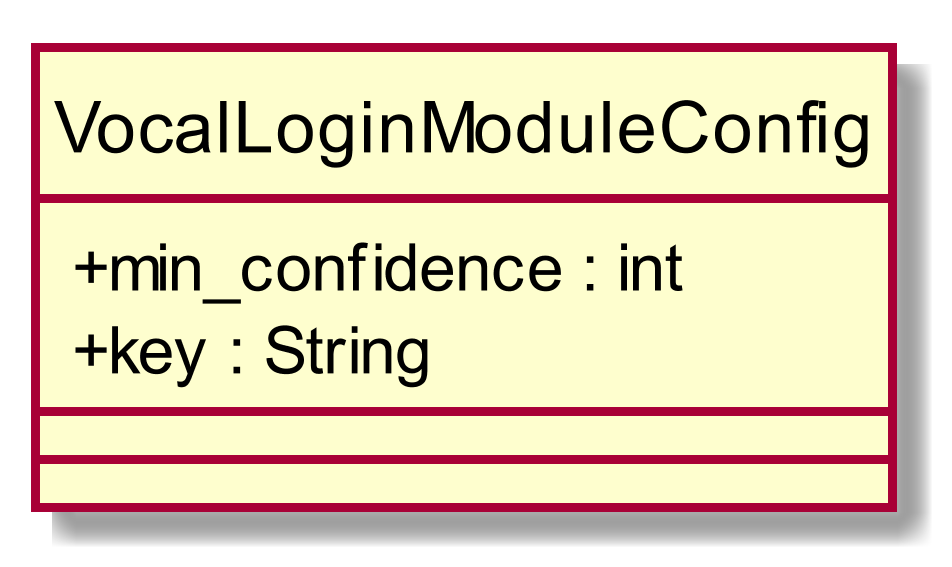
\includegraphics[width=\textwidth,height=\textheight,keepaspectratio]{images/ClassVocalLoginModuleConfig.png}
	\caption{Back-end::APIGateway::VocalLoginModuleConfig}
\end{figure}
\begin{itemize}
	\item \textbf{Nome}: \file{VocalLoginModuleConfig};
	\item \textbf{Tipo}: \file{Class};
	\item \textbf{Descrizione}: questa classe viene utilizzata per la configurazione di \file{VocalLoginModule};
	\item \textbf{Utilizzo}: fornisce gli attributi necessari alla configurazione di \file{VocalLoginModule};
	\item \textbf{Attributi}:
	\begin{itemize}
		\item[] \file{+ min\_confidence: int} \\
		Questo attributo indica la confidence minima richiesta perchè il login avvenga con successo;
	\end{itemize}
\end{itemize}

\subsection{Back-end::Auth}
Package contenente le componenti del microservizio necessario all'autenticazione.
\subsubsection{Classi}
\hypertarget{ UsersDAO_label}{\paragraph{ UsersDAO}}
\begin{figure}[h]
	\centering
	\includegraphics[width=\textwidth,height=\textheight,keepaspectratio]{images/Class UsersDAO.png}
	\caption{Back-end::Auth:: UsersDAO}
\end{figure}
\begin{itemize}
	\item \textbf{Nome}: \file{ UsersDAO};
	\item \textbf{Tipo}: \file{Interface};
	\item \textbf{Descrizione}: questa classe si occupa di astrarre le modalità d'interazione al database per questo microservizio. ;
	\item \textbf{Utilizzo}: fornisce a \file{UsersService} un meccanismo per accedere al database contenente gli utenti registrati, senza conoscerne le modalità di implementazione e di persistenza di quest'ultimo.
A partire da un identificativo, permette operazioni di lettura, scrittura e rimozione di utenti registrati;
	\item \textbf{Figlio}: \file{UsersDAODynamoDB};
	\item \textbf{Metodi}:
	\begin{itemize}
		\item[] \file{+ addUser(user: User): ErrorObservable} \\
		Metodo che permette di aggiungere un utente. \\
L'\file{Observable} restituito non riceverà alcun valore, ma verrà completato in caso di aggiunta dell'utente avvenuta con successo. In caso di errore durante l'aggiunta dell'utente, gli \file{Observer} interessati verranno notificati tramite la chiamata del loro metodo \file{error()} con i dati relativi all'errore verificatosi;\\
		Parametri:
		\begin{itemize}
			\item \file{user: User} \\
			Parametro contenente un utente registrato;
		\end{itemize}
		\item[] \file{+ removeUser(id: String): ErrorObservable} \\
		Metodo che permette di rimuovere un utente registrato. L'\file{Observable} restituito non riceverà alcun valore, ma verrà completato in caso di aggiunta dell'utente avvenuta con successo. In caso di errore durante l'aggiunta dell'utente, gli \file{Observer} interessati verranno notificati tramite la chiamata del loro metodo \file{error()} con i dati relativi all'errore verificatosi;\\
		Parametri:
		\begin{itemize}
			\item \file{id: String} \\
			Parametro contenente l'id dello \file{User} che si vuole eliminare;
		\end{itemize}
		\item[] \file{+ getUser(username: String): UserObservable} \\
		Metodo che permette di ottenere i dati relativi ad un utente. \\
L'\file{Observable} restituito riceverà l'oggetto rappresentante tale \file{User}, e verrà completato. Nel caso in cui l'utente richiesto non sia presente nel database, gli \file{Observer} interessati non riceveranno alcun valore, ma verranno notificati tramite la chiamata del loro metodo \file{error()};\\
		Parametri:
		\begin{itemize}
			\item \file{username: String} \\
			Parametro contenente lo username dello \file{User} che si vuole ottenere;
		\end{itemize}
		\item[] \file{+ getUserList(): UserObservable} \\
		L'\file{Observable} restituito manderà agli \file{Observer} gli utenti ottenuti, uno alla volta, e poi chiama il loro metodo \file{complete}. Nel caso in cui si verifichi un errore, gli \file{Observer} iscritti verranno notificati tramite la chiamate del loro metodo \file{error} con i dati relativi all'errore verificatosi;\\
		\item[] \file{+ updateUser(user: User): ErrorObservable} \\
		Metodo che permette di aggiornare un utente registrato.  L'\file{Observable} restituito non riceverà alcun valore, ma verrà completato in caso di aggiunta dell'utente avvenuta con successo. In caso di errore durante l'aggiunta dell'utente, gli \file{Observer} interessati verranno notificati tramite la chiamata del loro metodo \file{error()} con i dati relativi all'errore verificatosi;\\
		Parametri:
		\begin{itemize}
			\item \file{user: User} \\
			Parametro contenente lo \file{User} aggiornato;
		\end{itemize}
	\end{itemize}
\end{itemize}

\hypertarget{SRUser_label}{\paragraph{SRUser}}
\begin{figure}[h]
	\centering
	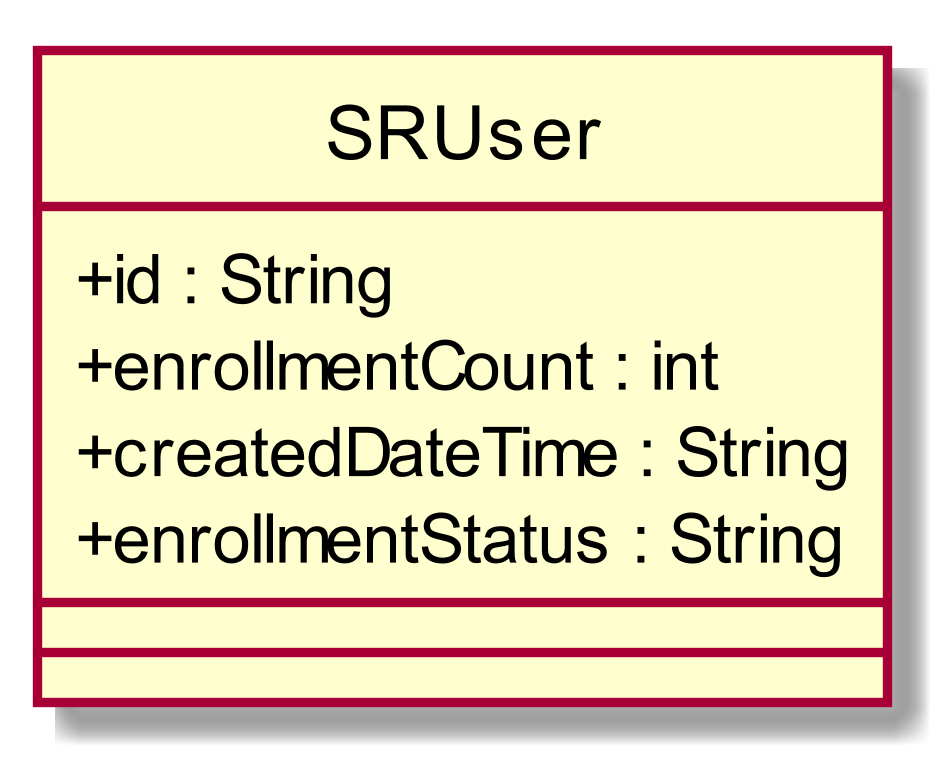
\includegraphics[width=\textwidth,height=\textheight,keepaspectratio]{images/ClassSRUser.png}
	\caption{Back-end::Auth::SRUser}
\end{figure}
\begin{itemize}
	\item \textbf{Nome}: \file{SRUser};
	\item \textbf{Tipo}: \file{Class};
	\item \textbf{Descrizione}: questa classe si occupa di rappresentare ed organizzare i parametri dell'autenticazione tramite Speaker Recognition (SR);
	\item \textbf{Utilizzo}: fornisce l'insieme dei parametri necessari ad identificare, tramite SR, un utente sottoposto alla procedura di Enrollment del servizio di Speaker Recognition.
Per la relativa documentazione consultare la pagina \url{https://www.microsoft.com/cognitive-services/en-us/speaker-recognition-api/documentation}.
;
	\item \textbf{Attributi}:
	\begin{itemize}
		\item[] \file{+ id: String} \\
		Attributo contenente l'identificativo del profilo utente del microservizio di Speaker Recognition;
		\item[] \file{+ enrollmentCount: int} \\
		Attributo contenente il numero di Enrollment dello \file{User};
		\item[] \file{+ createdDateTime: String} \\
		Attributo contenente la data di creazione del profilo utente nel microservizio esterno di Speaker Recognition;
		\item[] \file{+ enrollmentStatus: String} \\
		Attributo contenente lo stato dell'Enrollment.\\
Lo stato può essere uno tra i seguenti valori:
\begin{itemize} \item Enrolling: indica che la fase di enrollment è in corso; \item Training: indica che il microservizio di Speaker Recognition sta elaborando e organizzando i dati ricevuti (analizza le frasi comunicate e ne costruisce un'impronta vocale); \item Enrolled, ovvero che le due fasi precedenti sono state completate. \end{itemize};
	\end{itemize}
\end{itemize}

\hypertarget{User_label}{\paragraph{User}}
\begin{figure}[h]
	\centering
	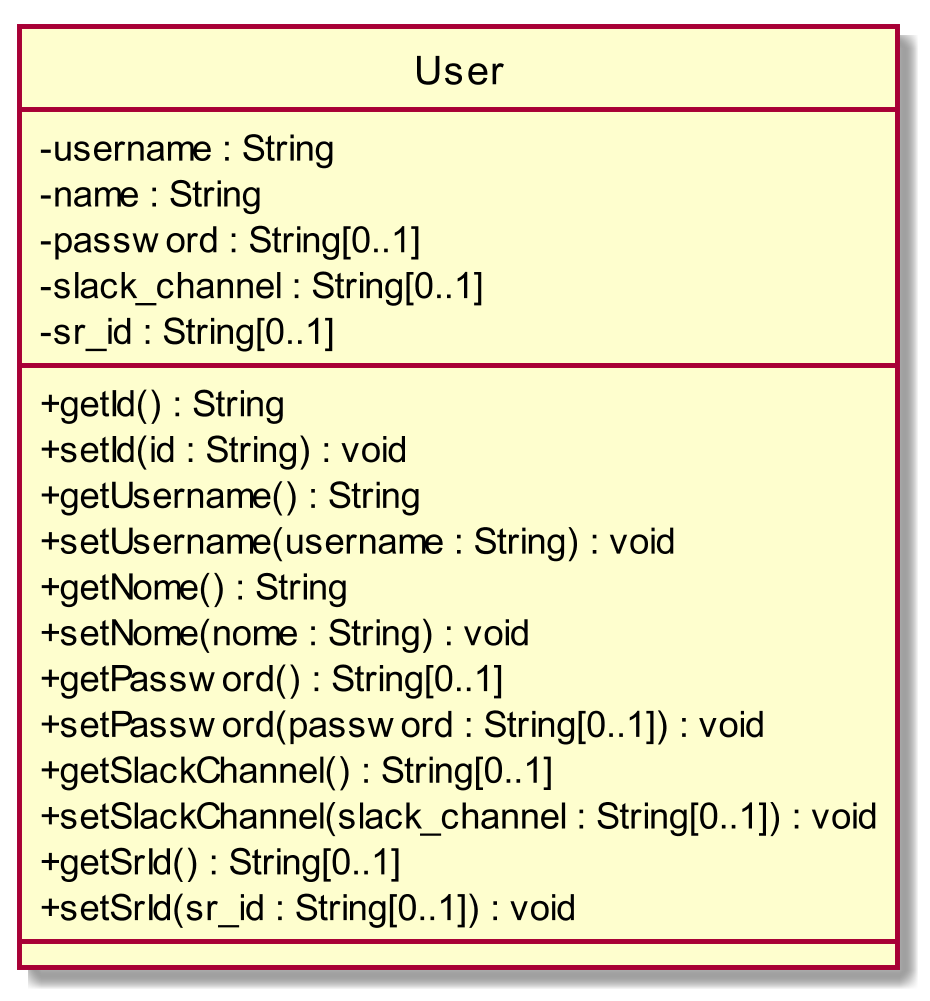
\includegraphics[width=\textwidth,height=\textheight,keepaspectratio]{images/ClassUser.png}
	\caption{Back-end::Auth::User}
\end{figure}
\begin{itemize}
	\item \textbf{Nome}: \file{User};
	\item \textbf{Tipo}: \file{Class};
	\item \textbf{Descrizione}: questa classe si occupa di rappresentare e organizzare i dati relativi ad un utente registrato;
	\item \textbf{Utilizzo}: fornisce i metodi getter e setter per i parametri relativi ad un utente registrato, i quali dovranno essere memorizzati nel database per questo microservizio.\\
È utilizzata dalla classe \file{UsersDAO} e dalle classi che utilizzano quest'ultima;
	\item \textbf{Attributi}:
	\begin{itemize}
		\item[] \file{- username: String} \\
		Attributo contenente l'username dell'utente registrato;
		\item[] \file{- first\_name: String} \\
		Attributo contenente il nome dell'utente registrato;
		\item[] \file{- last\_name: String} \\
		Attributo contenente il cognome dell'utente registrato;
		\item[] \file{- password: String[0..1]} \\
		Attributo contenente la password dell'utente registrato;
		\item[] \file{- slack\_channel: String[0..1]} \\
		Attributo contenente il canale Slack dell'utente registrato;
		\item[] \file{- sr\_id: String[0..1]} \\
		Attributo contenente l'id del profilo utente nel microservizio esterno di Speaker Recognition;
	\end{itemize}
	\item \textbf{Metodi}:
	\begin{itemize}
		\item[] \file{+ getId(): String} \\
		Metodo che permette di ottenere l'id dell'utente registrato;\\
		\item[] \file{+ setId(id: String): void} \\
		Metodo che permette di impostare l'id dell'utente registrato;\\
		Parametri:
		\begin{itemize}
			\item \file{id: String} \\
			Parametro contenente l'id;
		\end{itemize}
		\item[] \file{+ getUsername(): String} \\
		Metodo che permette di ottenere lo username dell'utente registrato;\\
		\item[] \file{+ setUsername(username: String): void} \\
		Metodo che permette di impostare lo username dell'utente registrato;\\
		Parametri:
		\begin{itemize}
			\item \file{username: String} \\
			Parametro relativo all'username da settare;
		\end{itemize}
		\item[] \file{+ getNome(): String} \\
		Metodo che permette di ottenere il nome dell'utente registrato;\\
		\item[] \file{+ setNome(nome: String): void} \\
		Metodo che permette di impostare il nome dell'utente registrato;\\
		Parametri:
		\begin{itemize}
			\item \file{nome: String} \\
			Parametro contenente il nome;
		\end{itemize}
		\item[] \file{+ getPassword(): String[0..1]} \\
		Metodo che permette di ottenere la password dell'utente registrato;\\
		\item[] \file{+ setPassword(password: String[0..1]): void} \\
		Metodo che permette di impostare la password dell'utente registrato;\\
		Parametri:
		\begin{itemize}
			\item \file{password: String[0..1]} \\
			Parametro relativo alla password da settare;
		\end{itemize}
		\item[] \file{+ getSlackChannel(): String[0..1]} \\
		Metodo che permette di ottenere il canale Slack dell'utente registrato;\\
		\item[] \file{+ setSlackChannel(slack\_channel: String[0..1]): void} \\
		Metodo che permette di impostare il canale Slack dell'utente registrato necessario per contattarlo;\\
		Parametri:
		\begin{itemize}
			\item \file{slack\_channel: String[0..1]} \\
			Parametro relativo al canale Slack da settare;
		\end{itemize}
		\item[] \file{+ getSrId(): String[0..1]} \\
		Metodo che permette di ottenere l'id del profilo utente nel microservizio esterno di Speaker Recognition;\\
		\item[] \file{+ setSrId(sr\_id: String[0..1]): void} \\
		Metodo che permette di impostare l'id dello Speaker Recognition associato all'utente registrato;\\
		Parametri:
		\begin{itemize}
			\item \file{sr\_id: String[0..1]} \\
			Parametro relativo all'id dello Speaker Recognition da settare;
		\end{itemize}
	\end{itemize}
\end{itemize}

\hypertarget{UsersDAODynamoDB_label}{\paragraph{UsersDAODynamoDB}}
\begin{figure}[h]
	\centering
	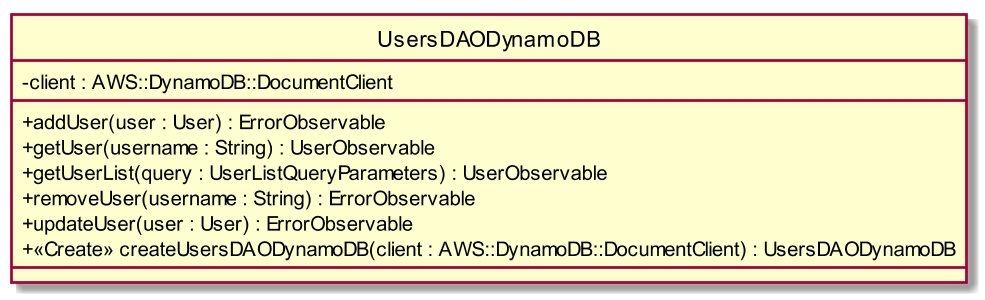
\includegraphics[width=\textwidth,height=\textheight,keepaspectratio]{images/ClassUsersDAODynamoDB.png}
	\caption{Back-end::Auth::UsersDAODynamoDB}
\end{figure}
\begin{itemize}
	\item \textbf{Nome}: \file{UsersDAODynamoDB};
	\item \textbf{Tipo}: \file{Class};
	\item \textbf{Descrizione}: classe che si occupa di implementare l'interfaccia \file{UsersDAO}, utilizzando un database DynamoDB come supporto per la memorizzazione dei dati;
	\item \textbf{Utilizzo}: implementa i metodi dell'interfaccia \file{UsersDAO} interrogando un database DynamoDB. Utilizza \file{AWS::DynamoDB::DocumentClient} per l'accesso al database. La dependency injection dell'oggetto \file{AWS::DynamoDB} viene fatta utilizzando il costruttore;
	\item \textbf{Padre}: \file{<<interface>> UsersDAO};
	\item \textbf{Attributi}:
	\begin{itemize}
		\item[] \file{- db: AWS::DynamoDB} \\
		Attributo contenente un riferimento al modulo di Node.js utilizzato per l'accesso al database DynamoDB contenente la tabella degli utenti;
	\end{itemize}
	\item \textbf{Metodi}:
	\begin{itemize}
		\item[] \file{+ addUser(user: User): ErrorObservable} \\
		Implementazione del metodo definito nell'interfaccia \file{UsersDAO}. Utilizza il metodo put del \file{DocumentClient} per aggiungere l'utente al database;\\
		Parametri:
		\begin{itemize}
			\item \file{user: User} \\
			Utente che si vuole aggiungere al sistema;
		\end{itemize}
		\item[] \file{+ getUser(username: String): UserObservable} \\
		Implementazione del metodo definito nell'interfaccia \file{UsersDAO}. Utilizza il metodo get del \file{DocumentClient} per ottenere i dati relativi ad uno \file{User} dal database;\\
		Parametri:
		\begin{itemize}
			\item \file{username: String} \\
			Parametro contenente lo username dello \file{User} che si vuole ottenere;
		\end{itemize}
		\item[] \file{+ getUserList(): UserObservable} \\
		Implementazione del metodo dell'interfaccia \file{UsersDAO}. Utilizza il metodo scan del \file{DocumentClient} per ottenere la lista degli utenti dal database;\\
		\item[] \file{+ removeUser(username: String): ErrorObservable} \\
		Implementazione del metodo dell'interfaccia \file{UsersDAO}. Utilizza il metodo delete del \file{DocumentClient} per eliminare un utente dal database;\\
		Parametri:
		\begin{itemize}
			\item \file{username: String} \\
			Usernaname dell'utente che si vuole rimuovere dal sistema;
		\end{itemize}
		\item[] \file{+ updateUser(user: User): ErrorObservable} \\
		Implementazione del metodo dell'interfaccia \file{UsersDAO}. Utilizza il metodo update del \file{DocumentClient} per aggiornare i dati relativi ad un utente presente all'interno del database;\\
		Parametri:
		\begin{itemize}
			\item \file{user: User} \\
			Parametro contenente i dati relativi all'utente che si vuole modificare;
		\end{itemize}
		\item[] \file{+ <<Create>> createUsersDAODynamoDB(db : AWS::DynamoDB): UsersDAODynamoDB} \\
		Constructor della classe \file{UsersDAODynamoDB}. Permette di effettuare la dependency injection di \file{AWS::DynamoDB};\\
		Parametri:
		\begin{itemize}
			\item \file{db : AWS::DynamoDB} \\
			Parametro contenente un riferimento al modulo di Node.js da utilizzare per l'accesso al database DynamoDB contenente la tabella degli utenti;
		\end{itemize}
	\end{itemize}
\end{itemize}

\hypertarget{UsersService_label}{\paragraph{UsersService}}
\begin{figure}[h]
	\centering
	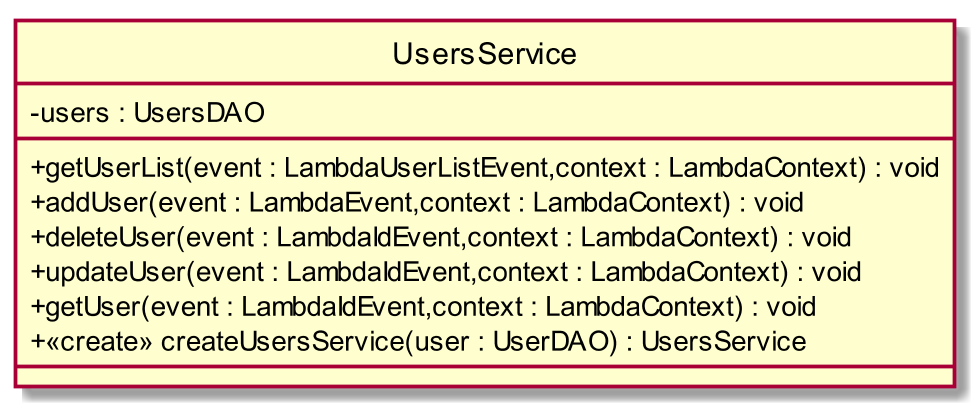
\includegraphics[width=\textwidth,height=\textheight,keepaspectratio]{images/ClassUsersService.png}
	\caption{Back-end::Auth::UsersService}
\end{figure}
\begin{itemize}
	\item \textbf{Nome}: \file{UsersService};
	\item \textbf{Tipo}: \file{Class};
	\item \textbf{Descrizione}: questa classe si occupa di realizzare il microservizio \file{Auth} e, tramite \file{UsersDAO}, di interagire con il database degli utenti registrati;
	\item \textbf{Utilizzo}: fornisce i metodi che implementano le lambda function necessarie alla gestione degli utenti.
Questa classe non interagisce direttamente con il database, ma fa utilizzo di \file{UsersDAO}, il quale nasconde i meccanismi di accesso e persistenza dei dati nel database;
	\item \textbf{Attributi}:
	\begin{itemize}
		\item[] \file{- users: UsersDAO} \\
		Attributo che permette di contattare \file{UsersDAO}, il quale fornisce i meccanismi d'accesso al database degli utenti registrati;
	\end{itemize}
	\item \textbf{Metodi}:
	\begin{itemize}
		\item[] \file{+ getUserList(event: LambdaEvent, context: LambdaContext): void} \\
		Metodo che implementa la lambda function che si occupa di restituire l'array degli utenti registrati;\\
		Parametri:
		\begin{itemize}
			\item \file{event: LambdaEvent} \\
			Parametro che rappresenta la richiesta ricevuta dal \file{VocalAPI}. Il campo \file{body} di questo attributo conterrà una stringa vuota;
			\item \file{context: LambdaContext} \\
			Parametro utilizzato dalle lambda function per inviare la risposta. Il \file{body} del \file{LambdaResponse}, ottenuto dal metodo \file{LambdaContext::succeed}, conterrà un Array di oggetti di tipo \file{User};
		\end{itemize}
		\item[] \file{+ addUser(event: LambdaEvent, context: LambdaContext): void} \\
		Metodo che implementa la lambda function che si occupa di aggiungere un utente registrato;\\
		Parametri:
		\begin{itemize}
			\item \file{event: LambdaEvent} \\
			Parametro contenente, all'interno del campo \file{body} sotto forma di stringa in formato JSON, un oggetto \file{User} contenente tutti i dati relativi ad un utente da inserire;
			\item \file{context: LambdaContext} \\
			Parametro utilizzato dalle lambda function per inviare la risposta. La risposta, contenuta nel \file{LambdaResponse} parametro del metodo \file{LambdaContext::succeed}, possiede un attributo \file{body}, il quale conterrà una stringa vuota. Il risultato delle operazioni di questo metodo sarà deducibile tramite il valore dell'attributo \file{LambaResponse::statusCode};
		\end{itemize}
		\item[] \file{+ removeUser(event: LambdaIdEvent, context: LambdaContext): void} \\
		Metodo che implementa la lambda function che si occupa di rimuovere un utente registrato;\\
		Parametri:
		\begin{itemize}
			\item \file{event: LambdaIdEvent} \\
			Parametro contenente, all'interno del campo \file{pathParameters}, lo username dell'utente registrato che si vuole eliminare;
			\item \file{context: LambdaContext} \\
			Parametro utilizzato dalle lambda function per inviare la risposta. Il \file{body} del \file{LambdaResponse}, parametro del metodo \file{LambdaContext::succeed}, conterrà una stringa vuota e il risultato di questa operazione sarà deducibile dal valore dell'attributo \file{LambaResponse::statusCode};
		\end{itemize}
		\item[] \file{+ updateUser(event: LambdaIdEvent, context: LambdaContext): void} \\
		Metodo che implementa la lambda function che si occupa di aggiornare i dati di un utente registrato;\\
		Parametri:
		\begin{itemize}
			\item \file{event: LambdaIdEvent} \\
			Parametro contenente all'interno del campo \file{body}, sotto forma di stringa in formato JSON, un oggetto di tipo \file{User} contente i dati da aggiornare e, all'interno del campo \file{pathParameters}, lo username dell'utente da modificare;
			\item \file{context: LambdaContext} \\
			Parametro utilizzato dalle lambda function per inviare la risposta. Il \file{body} del \file{LambdaResponse}, parametro del metodo \file{LambdaContext::succeed}, conterrà una stringa vuota e il risultato di questa operazione sarà deducibile dal valore dell'attributo \file{LambaResponse::statusCode};
		\end{itemize}
		\item[] \file{+ getUser(event: LambdaIdEvent, context: LambdaContext): void} \\
		Metodo che implementa la lambda function che si occupa di restituire i dati relativi ad un utente a partire dal suo username;\\
		Parametri:
		\begin{itemize}
			\item \file{event: LambdaIdEvent} \\
			Parametro contenente, all'interno del campo \file{pathParameters}, lo username dell'utente registrato del quale si vogliono ottenere i dati;
			\item \file{context: LambdaContext} \\
			Parametro utilizzato dalle lambda function per inviare la risposta. Il \file{body} del \file{LambdaResponse}, parametro del metodo \file{LambdaContext::succeed}, conterrà un oggetto , sotto forma di stringa in formato JSON, di tipo \file{User}, contenente i dati relativi all'utente ritornato;
		\end{itemize}
		\item[] \file{+ <<create>> createUsersService(user: UserDAO): UsersService} \\
		Metodo che permette di creare uno \file{UsersService}. Permette la dependency injection avente come oggetto uno \file{UsersDAO};\\
		Parametri:
		\begin{itemize}
			\item \file{user: UserDAO} \\
			Attributo contenente lo \file{UsersDAO};
		\end{itemize}
	\end{itemize}
\end{itemize}

\hypertarget{VocalLoginModule_label}{\paragraph{VocalLoginModule}}
\begin{figure}[h]
	\centering
	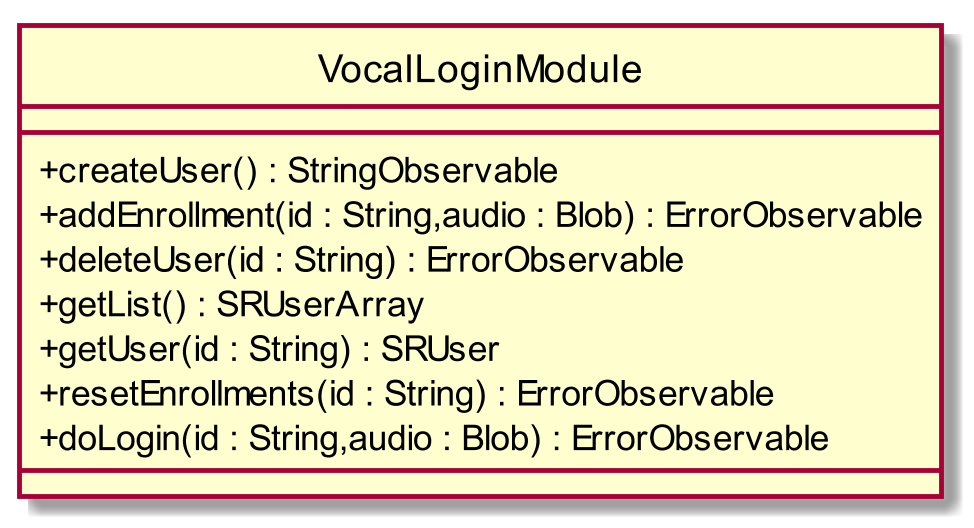
\includegraphics[width=\textwidth,height=\textheight,keepaspectratio]{images/ClassVocalLoginModule.png}
	\caption{Back-end::Auth::VocalLoginModule}
\end{figure}
\begin{itemize}
	\item \textbf{Nome}: \file{VocalLoginModule};
	\item \textbf{Tipo}: \file{Class};
	\item \textbf{Descrizione}: questa classe si occupa di realizzare e raggruppare tutte le operazioni necessarie all'identificazione di un utente registrato, tramite il microservizio di Speaker Recognition (SR). ;
	\item \textbf{Utilizzo}: fornisce un meccanismo per creare, eliminare ed ottenere un utente registrato associato ad un Enrollment, il quale è necessario all'identificazione di un utente tramite il microservizio di Speak Recognition (SR). Permette quindi di associare i parametri relativi ad un \file{Enrollment} ad un utente registrato.\\
È soggetta ad una constructor-based dependency injection, la quale ha come oggetto un \file{VocalLoginModulConfig};
	\item \textbf{Attributi}:
	\begin{itemize}
		\item[] \file{- min\_confidence: int} \\
		Attributo contenente il grado di confidenza minimo accettabile nel confronto tra ciò che l'utente comunica, al fine di effettuare l'accesso come utente registrato, e quella che dovrebbe essere la sua impronta vocale precedentemente costruita tramite il meccanismo di Enrollment;
	\end{itemize}
	\item \textbf{Metodi}:
	\begin{itemize}
		\item[] \file{+ createUser(): String} \\
		Metodo che permette di creare un User;\\
		\item[] \file{+ <<Create>> createVocalLoginModule(conf: VocalLoginModuleConfig): VocalLoginModule} \\
		Metodo che permette di costruire un \file{VocalLoginModule}. Permette la dependency injection che ha come oggetto un \file{VocalLoginModuleConfig};\\
		Parametri:
		\begin{itemize}
			\item \file{conf: VocalLoginModuleConfig} \\
			Parametro attraverso il quale viene passata la configurazione di VocalLoginModule;
		\end{itemize}
		\item[] \file{+ addEnrollment(id: String, audio: Blob): Error} \\
		Metodo che permette di aggiungere un Enrollment;\\
		Parametri:
		\begin{itemize}
			\item \file{id: String} \\
			Parametro relativo a ????;
			\item \file{audio: Blob} \\
			Parametro contenente l'audio relativo alla frase di riconoscimento pronunciata;
		\end{itemize}
		\item[] \file{+ deleteUser(id: String): Error} \\
		Metodo che permette di eliminare un User a partire da un id;\\
		Parametri:
		\begin{itemize}
			\item \file{id: String} \\
			Parametro relativo a ??;
		\end{itemize}
		\item[] \file{+ getList(): SRUserArray} \\
		Metodo che ritorna una lista di SRUser;\\
		\item[] \file{+ getUser(id: String): SRUser} \\
		Metodo che ritorna un SRUser a partire da un id;\\
		Parametri:
		\begin{itemize}
			\item \file{id: String} \\
			Parametro contenente l'identificativo dello \file{User};
		\end{itemize}
		\item[] \file{+ resetEnrollments(id: String): Error} \\
		Metodo che permette di resettare un enrollment a partire da un id;\\
		Parametri:
		\begin{itemize}
			\item \file{id: String} \\
			Parametro relativo a ???;
		\end{itemize}
		\item[] \file{+ doLogin(id: String, audio: Blob): Error} \\
		Metodo che permette di effettuare il login a partire da un id e da un audio di identificazione;\\
		Parametri:
		\begin{itemize}
			\item \file{id: String} \\
			Parametro contenente l'identificativo ???;
			\item \file{audio: Blob} \\
			Parametro contenente l'audio relativo alla frase di riconoscimento pronunciata;
		\end{itemize}
	\end{itemize}
\end{itemize}

\subsection{Back-end::Notifications}
Package che contiene le componenti relative al microservizio che si occupa delle notifiche.
\subsubsection{Classi}
\hypertarget{Action_label}{\paragraph{Action}}
\begin{figure}[h]
	\centering
	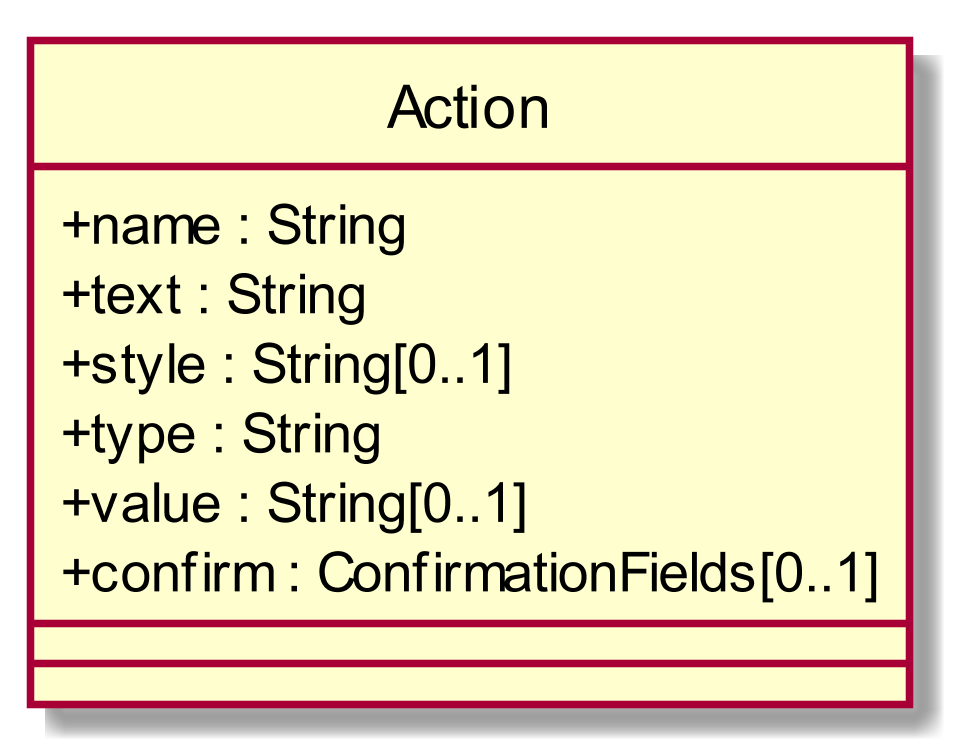
\includegraphics[width=\textwidth,height=\textheight,keepaspectratio]{images/ClassAction.png}
	\caption{Back-end::Notifications::Action}
\end{figure}
\begin{itemize}
	\item \textbf{Nome}: \file{Action};
	\item \textbf{Tipo}: \file{Class};
	\item \textbf{Descrizione}: questa classe si occupa di rappresentare e organizzare gli attributi relativi ad una \file{Action} come descritto nelle API di Slack. Rappresenta un button in un messaggio Slack;
	\item \textbf{Utilizzo}: fornisce gli attributi di una \file{Action}. La classe \file{Attachment} ne contiene un array.
Per la relativa documentazione, consultare la pagina \url{https://api.slack.com/docs/message-buttons};
	\item \textbf{Attributi}:
	\begin{itemize}
		\item[] \file{+ name: String} \\
		Attributo contenente il nome dell'azione. Se ci sono più azioni con lo stesso nome, solo una di esse può essere in uno stato attivato;
		\item[] \file{+ text: String} \\
		Attributo contenente il testo del bottone dell'azione;
		\item[] \file{+ style: String[0..1]} \\
		Attributo che definisce lo stile del bottone. Per una lista degli stili disponibili e una loro descrizione fare riferimento alla documentazione di Slack (\url{https://api.slack.com/docs/message-buttons#action_fields});
		\item[] \file{+ type: String} \\
		Attributo contenente il tipo dell'azione. Al momento l'unico valore accettato è "button". Fare riferimento alle API di   Slack per informazioni aggiornate (\url{https://api.slack.com/docs/message-buttons#action_fields}). ;
		\item[] \file{+ value: String[0..1]} \\
		Attributo contenente il valore dell'azione. Se sono presenti diverse azioni con lo stesso nome, può essere utilizzato per distinguere diversi intenti;
		\item[] \file{+ confirm: ConfirmationFields[0..1]} \\
		Attributo contenete i dati relativi al dialogo di conferma, che nel caso di bottoni con azioni che possono avere effetti particolarmente "distruttivi" permette di chiedere un'ulteriore conferma prima di compiere effettivamente tali azioni;
	\end{itemize}
\end{itemize}

\hypertarget{Attachment_label}{\paragraph{Attachment}}
\begin{figure}[h]
	\centering
	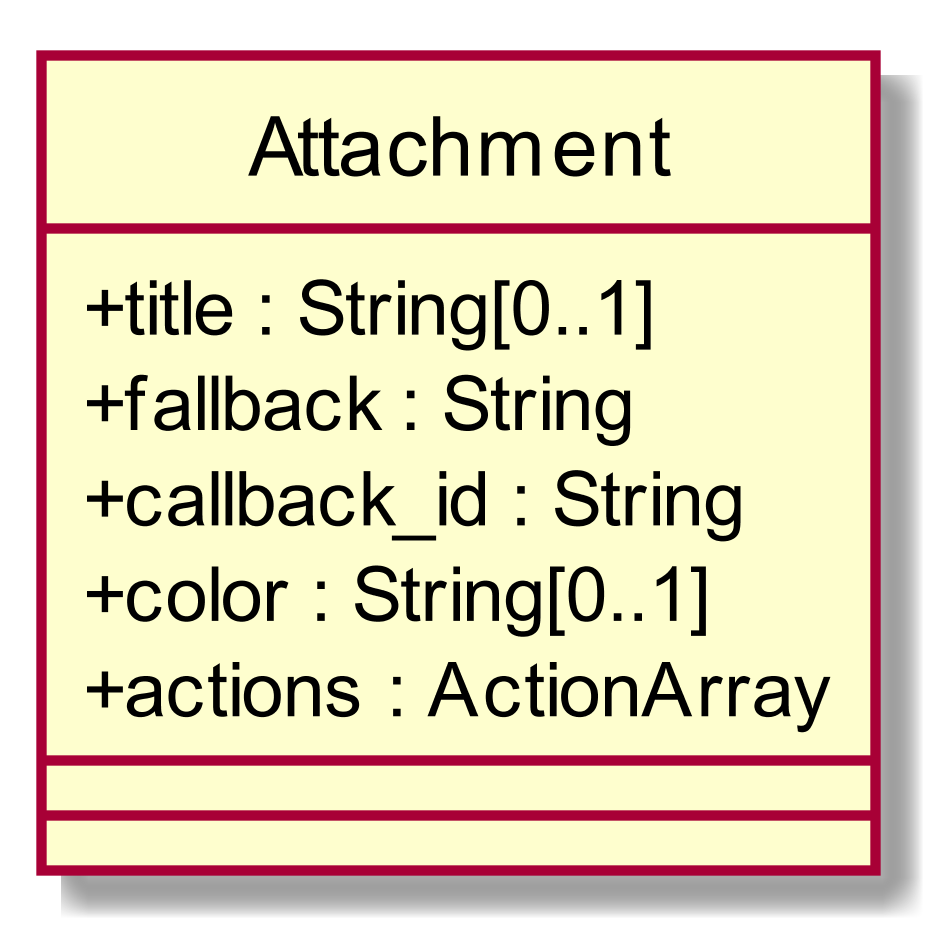
\includegraphics[width=\textwidth,height=\textheight,keepaspectratio]{images/ClassAttachment.png}
	\caption{Back-end::Notifications::Attachment}
\end{figure}
\begin{itemize}
	\item \textbf{Nome}: \file{Attachment};
	\item \textbf{Tipo}: \file{Class};
	\item \textbf{Descrizione}: questa classe si occupa di rappresentare e organizzare i dati relativi ad un Attachment.
;
	\item \textbf{Utilizzo}: fornisce gli attributi degli Attachment che dovranno essere aggiunti ad un NotificationMessage.
Un Attachment, contenuto in un NotificationsMessage, permette di aggiungere del significato ad un NotificationMessage ed arricchirlo tramite immagini, colori ed altro.
Per la relativa documentazione, consultare questa pagina \url{https://api.slack.com/docs/message-buttons};
	\item \textbf{Attributi}:
	\begin{itemize}
		\item[] \file{+ title: String[0..1]} \\
		Attributo contenente il titolo dell'attachment;
		\item[] \file{+ fallback: String} \\
		Attributo contenente un messaggio mostrato agli utenti che utilizzano un'interfaccia che non supporta gli attachments;
		\item[] \file{+ callback\_id: String} \\
		Attributo contenente l'id della collezione di bottoni all'interno dell'attachment;
		\item[] \file{+ color: String[0..1]} \\
		Attributo contenente il colore dell'attachment;
		\item[] \file{+ actions: ActionArray} \\
		Attributo contenente una array di \file{Action} da includere nell'attachment. Questo array può contenere al massimo cinque \file{Action};
	\end{itemize}
\end{itemize}

\hypertarget{ConfirmationFields_label}{\paragraph{ConfirmationFields}}
\begin{figure}[h]
	\centering
	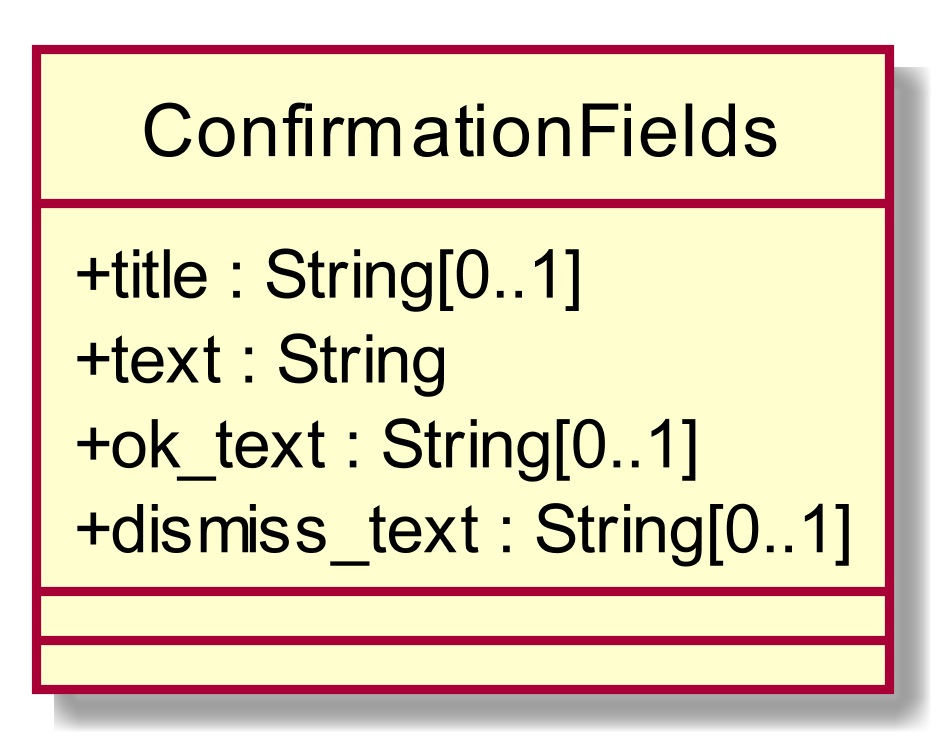
\includegraphics[width=\textwidth,height=\textheight,keepaspectratio]{images/ClassConfirmationFields.png}
	\caption{Back-end::Notifications::ConfirmationFields}
\end{figure}
\begin{itemize}
	\item \textbf{Nome}: \file{ConfirmationFields};
	\item \textbf{Tipo}: \file{Class};
	\item \textbf{Descrizione}: questa classe si occupa di rappresentare e organizzare gli attributi relativi ad un messaggio di conferma di Slack;
	\item \textbf{Utilizzo}: fornisce gli attributi per rappresentare un messaggio di conferma di Slack.
\\
Per la relativa documentazione, consultare la pagina \url{https://api.slack.com/docs/message-buttons};
	\item \textbf{Attributi}:
	\begin{itemize}
		\item[] \file{+ title: String[0..1]} \\
		Attributo contenente il titolo della finestra di pop up;
		\item[] \file{+ text: String} \\
		Attributo contenente la descrizione dettagliata delle conseguenze della relativa \file{Action} e contestualizza le scelte fornite dal button;
		\item[] \file{+ ok\_text: String[0..1]} \\
		Attributo contenente il testo del bottone che serve per confermare la relativa \file{Action}. Il valore di default per questo attributo è "Okay".
;
		\item[] \file{+ dismiss\_text: String[0..1]} \\
		Attributo contenente il testo del bottone che serve per cancellare la relativa \file{Action}. Il valore di default per questo attributo è "Cancel". ;
	\end{itemize}
\end{itemize}

\hypertarget{NotificationChannel_label}{\paragraph{NotificationChannel}}
\begin{figure}[h]
	\centering
	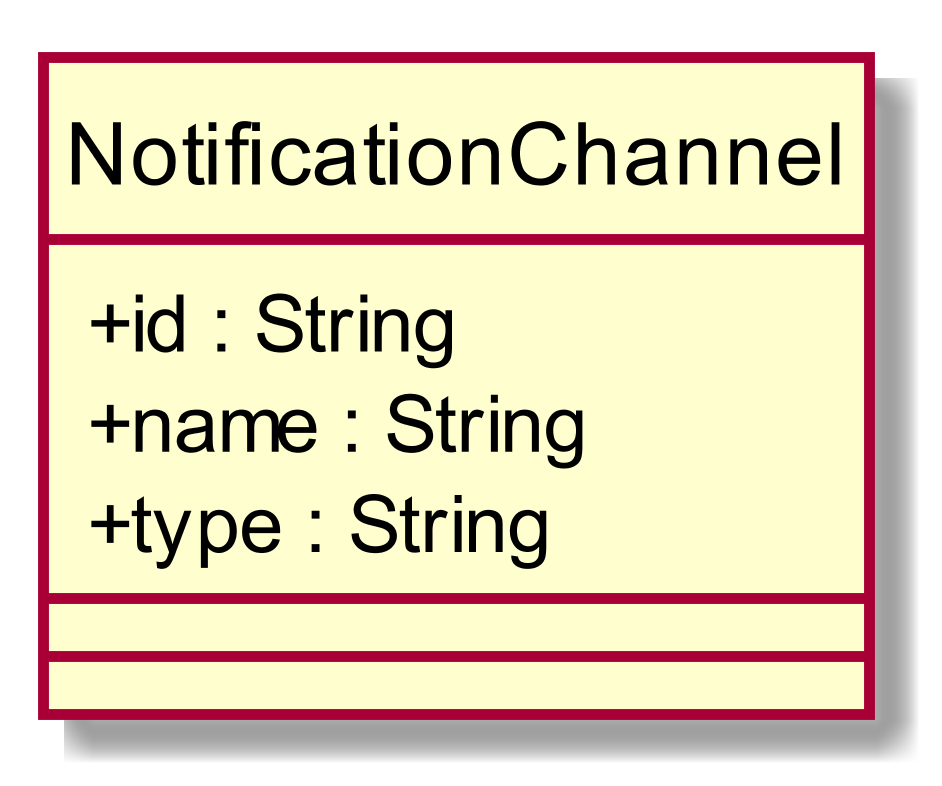
\includegraphics[width=\textwidth,height=\textheight,keepaspectratio]{images/ClassNotificationChannel.png}
	\caption{Back-end::Notifications::NotificationChannel}
\end{figure}
\begin{itemize}
	\item \textbf{Nome}: \file{NotificationChannel};
	\item \textbf{Tipo}: \file{Class};
	\item \textbf{Descrizione}: questa classe si occupa di rappresentare e organizzare i parametri relativi al canale Slack nel quale spedire il NotificationMessage;
	\item \textbf{Utilizzo}: fornisce gli attributi di un NotificationChannel. \\
Per consultare la relativa documentazione, consultare questa pagina \url{https://api.slack.com/types/channel};
	\item \textbf{Attributi}:
	\begin{itemize}
		\item[] \file{+ id: String} \\
		Attributo contenente l'id del canale Slack;
		\item[] \file{+ name: String} \\
		Attributo contenente il nome del canale Slack;
		\item[] \file{+ created: String} \\
		Attributo contenente l'unix timestamp relativo a creator;
		\item[] \file{+ creator: String} \\
		Attributo contenente l'id dell'utente Slack  che ha creato il canale Slack;
		\item[] \file{+ is\_archived: boolean} \\
		Attributo contenente un valore che permette di capire se un canale è stato archiviato o meno.
Un canale è archiviato se non è più parte delle conversazioni attive;
		\item[] \file{+ is\_member: boolean} \\
		Attributo contenente un valore booleano che permette di capire se il membro chiamante fa parte del canale Slack;
		\item[] \file{+ num\_members: int} \\
		Attributo contenente il numero dei partecipanti al canale Slack;
		\item[] \file{+ topic: Topic} \\
		Attributo contenente l'argomento di discussione del canale Slack;
		\item[] \file{+ purpose: Purpose} \\
		Attributo contenente lo scopo per il quale il canale Slack è stato creato;
	\end{itemize}
\end{itemize}

\hypertarget{NotificationMessage_label}{\paragraph{NotificationMessage}}
\begin{figure}[h]
	\centering
	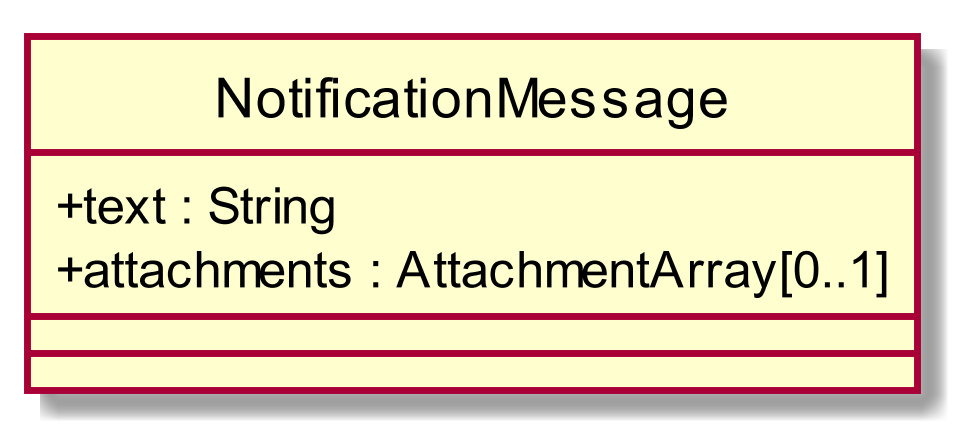
\includegraphics[width=\textwidth,height=\textheight,keepaspectratio]{images/ClassNotificationMessage.png}
	\caption{Back-end::Notifications::NotificationMessage}
\end{figure}
\begin{itemize}
	\item \textbf{Nome}: \file{NotificationMessage};
	\item \textbf{Tipo}: \file{Class};
	\item \textbf{Descrizione}: questa classe si occupa di rappresentare e organizzare i parametri relativi al messaggio da spedire nel NotificationChannel;
	\item \textbf{Utilizzo}: fornisce gli attributi di un NotificationChannel. \\ Per consultare la relativa documentazione, consultare questa pagina \url{https://api.slack.com/docs/message-formatting};
	\item \textbf{Attributi}:
	\begin{itemize}
		\item[] \file{+ text: String} \\
		Attributo contenente il testo del NotificationMessage;
		\item[] \file{+ attachments: AttachmentArray[0..1]} \\
		Attributo contenente l'array degli attachments del NotificationMessage;
		\item[] \file{+ response\_type: String[0..1]} \\
		Attributo contenente il modo con il quale notificare.
Questo attributo può assumere uno tra i seguenti valori:
\begin{itemize}
\item \file{in\_channel}, che mostra il \file{NotificationMessage} ai membri del canale con il message button già cliccato;
\item \file{ephemeral}, che mostra il \file{NotificationMessage} ai membri del canale che cliccano sul message button.
\end{itemize}
Per la relativa documentazione, consultare questa pagina \url{https://api.slack.com/docs/message-buttons};
	\end{itemize}
\end{itemize}

\hypertarget{NotificationService_label}{\paragraph{NotificationService}}
\begin{figure}[h]
	\centering
	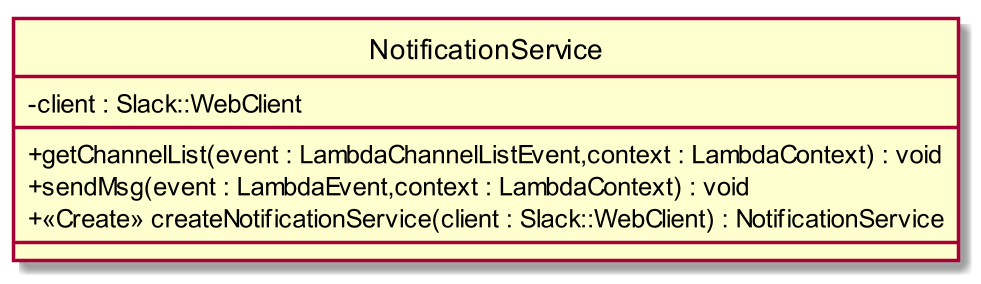
\includegraphics[width=\textwidth,height=\textheight,keepaspectratio]{images/ClassNotificationService.png}
	\caption{Back-end::Notifications::NotificationService}
\end{figure}
\begin{itemize}
	\item \textbf{Nome}: \file{NotificationService};
	\item \textbf{Tipo}: \file{Class};
	\item \textbf{Descrizione}: questa classe si occupa di realizzare il microservizio \file{Notifications};
	\item \textbf{Utilizzo}: fornisce i metodi che implementano le lambda function necessarie per notificare la persona desiderata sul relativo canale Slack;
	\item \textbf{Attributi}:
	\begin{itemize}
		\item[] \file{- BOT\_TOKEN: String} \\
		Attributo utilizzato per autenticarsi come bot;
	\end{itemize}
	\item \textbf{Metodi}:
	\begin{itemize}
		\item[] \file{+ getChannelList(event: LambdaEvent, context: LambdaContext): void} \\
		Metodo che implementa la lambda function che si occupa di restituire l'array dei canali Slack disponibili. ;\\
		Parametri:
		\begin{itemize}
			\item \file{event: LambdaEvent} \\
			Parametro che rappresenta la richiesta ricevuta dal \file{VocalAPI}. Il campo \file{body} di questo attributo conterrà una stringa vuota;
			\item \file{context: LambdaContext} \\
			Parametro utilizzato dalle lambda function per inviare la risposta. Il \file{body} del \file{LambdaResponse}, parametro del metodo \file{LambdaContext::succeed}, conterrà un Array di oggetti di tipo \file{NotificationChannel};
		\end{itemize}
		\item[] \file{+ sendMsg(event: LambdaEvent, context: LambdaContext): Msg} \\
		Metodo che implementa la lambda function che si occupa di inviare il messaggio alla persona desiderata;\\
		Parametri:
		\begin{itemize}
			\item \file{event: LambdaEvent} \\
			Parametro contenente, all'interno del campo \file{body} sotto forma di stringa in formato JSON, un oggetto contenente tutti i dati relativi ad un messaggio da inviare.
Tali dati sono:
\begin{lstlisting}[language=json,firstnumber=1]
{
    "msg":"NotificationMessage",
    "send\_to":"String"
}
\end{lstlisting}
Dove \file{msg} è un oggetto di tipo \file{NotificationMessage}, mentre \file{send\_to} è una stringa contenente il mittente del messaggio;
			\item \file{context: LambdaContext} \\
			Parametro utilizzato dalle lambda function per inviare la risposta. La risposta, contenuta nel \file{LambdaResponse} parametro del metodo \file{LambdaContext::succeed}, possiede un attributo \file{body}, il quale conterrà una stringa vuota. Il risultato delle operazioni di questo metodo sarà deducibile tramite il valore dell'attributo \file{LambaResponse::statusCode};
		\end{itemize}
	\end{itemize}
\end{itemize}

\hypertarget{Purpose_label}{\paragraph{Purpose}}
\begin{figure}[h]
	\centering
	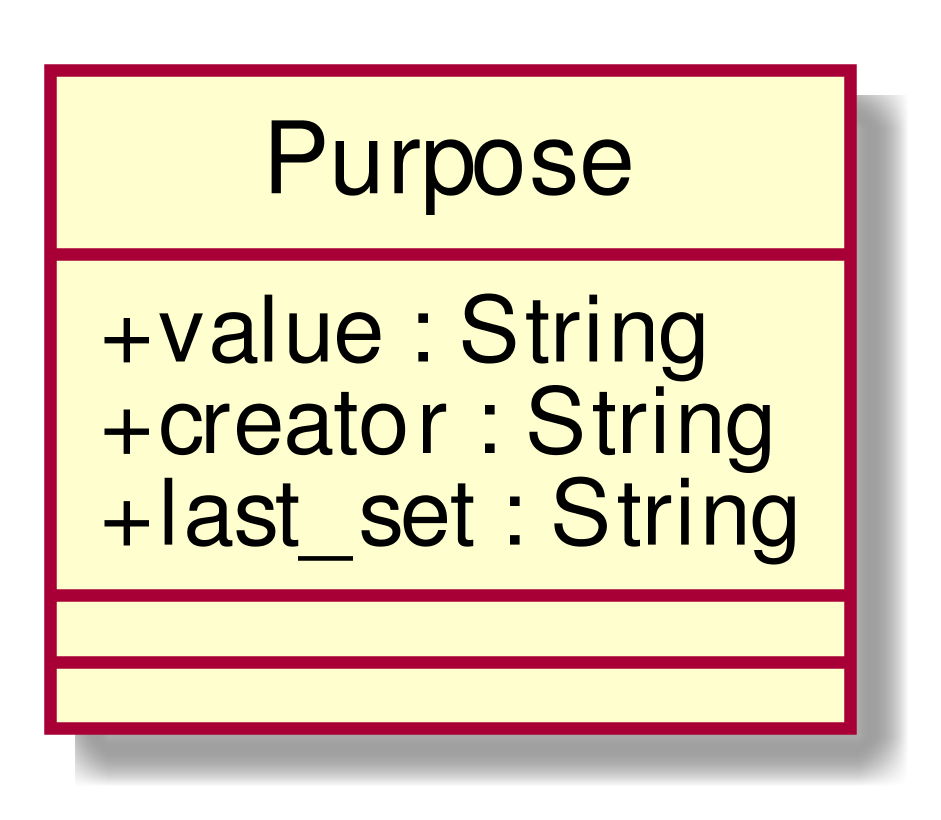
\includegraphics[width=\textwidth,height=\textheight,keepaspectratio]{images/ClassPurpose.png}
	\caption{Back-end::Notifications::Purpose}
\end{figure}
\begin{itemize}
	\item \textbf{Nome}: \file{Purpose};
	\item \textbf{Tipo}: \file{Class};
	\item \textbf{Descrizione}: questa classe si occupa di rappresentare e organizzare i dati relativi al Purpose di un canale Slack.
;
	\item \textbf{Utilizzo}: fornisce un meccanismo per impostare e ottenere i valori dei parametri relativi ad un Purpose.
Il purpose di un canale Slack è lo scopo per il quale è stato creato.
Per la relativa documentazione, consultare la seguente pagina \url{https://api.slack.com/methods/channels.setPurpose};
	\item \textbf{Attributi}:
	\begin{itemize}
		\item[] \file{+ value: String} \\
		Attributo contenente il valore del Purpose;
		\item[] \file{+ creator: String} \\
		Attributo contenente l'id del creatore dello scopo del canale Slack;
		\item[] \file{+ last\_set: String} \\
		Attributo contenente un unix timestamp relativo all'ultima modifica;
	\end{itemize}
\end{itemize}

\hypertarget{Topic_label}{\paragraph{Topic}}
\begin{figure}[h]
	\centering
	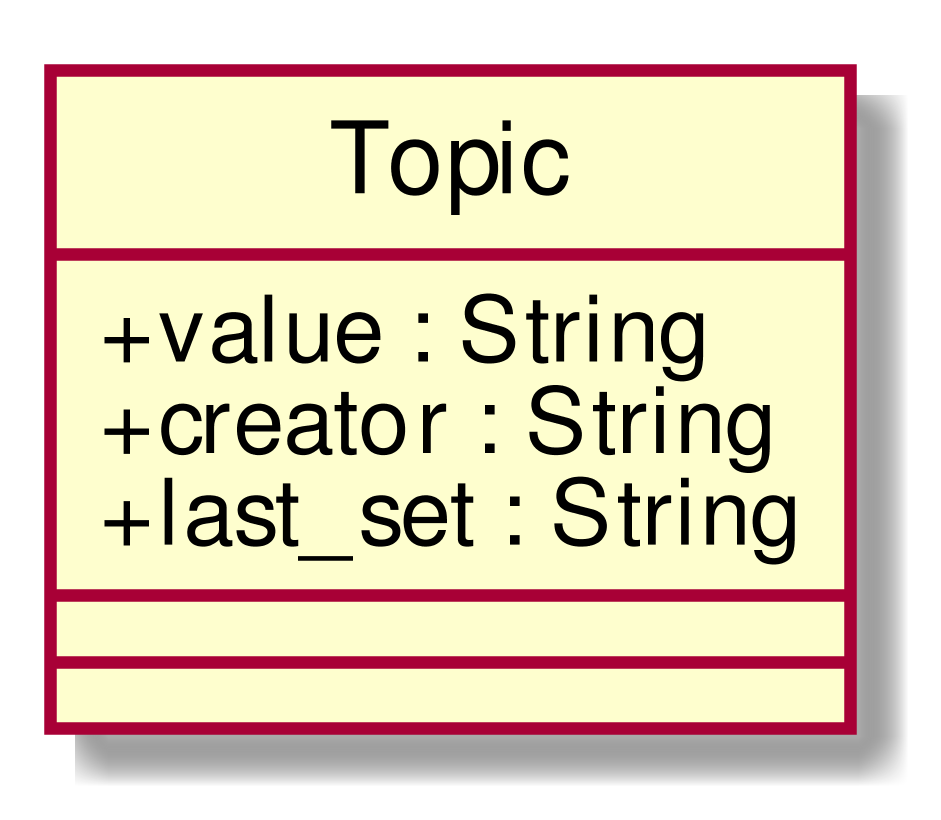
\includegraphics[width=\textwidth,height=\textheight,keepaspectratio]{images/ClassTopic.png}
	\caption{Back-end::Notifications::Topic}
\end{figure}
\begin{itemize}
	\item \textbf{Nome}: \file{Topic};
	\item \textbf{Tipo}: \file{Class};
	\item \textbf{Descrizione}: questa classe si occupa di rappresentare e organizzare i dati relativi al Topic di un canale Slack;
	\item \textbf{Utilizzo}: fornisce gli attributi del topic di un canale Slack.
Il Topic di un canale Slack è l'oggetto o tema delle discussioni in esso.
Per la relativa documentazione, consultare questa pagina \url{https://api.slack.com/methods/channels.setTopic};
	\item \textbf{Attributi}:
	\begin{itemize}
		\item[] \file{+ value: String} \\
		Attributo contenente il valore del Topic;
		\item[] \file{+ creator: String} \\
		Attributo contenente l'id del creatore del topic del canale Slack;
		\item[] \file{+ last\_set: String} \\
		Attributo contenente un unix timestamp relativo all'ultima modifica;
	\end{itemize}
\end{itemize}

\subsection{Back-end::Rules}
Package che contiene le componenti necessarie alla gestione delle impostazioni (direttive) dell'assistente virtuale.
\subsubsection{Classi}
\hypertarget{ RulesDAO_label}{\paragraph{ RulesDAO}}
\begin{figure}[h]
	\centering
	\includegraphics[width=\textwidth,height=\textheight,keepaspectratio]{images/Class RulesDAO.png}
	\caption{Back-end::Rules:: RulesDAO}
\end{figure}
\begin{itemize}
	\item \textbf{Nome}: \file{ RulesDAO};
	\item \textbf{Tipo}: \file{Interface};
	\item \textbf{Descrizione}: questa classe si occupa di astrarre le modalità di accesso al database per questo microservizio, contenente le Rule;
	\item \textbf{Utilizzo}: fornisce a \file{RuleService} un meccanismo per accedere al database, contenente le \file{Rule}, senza conoscerne le modalità di implementazioni e di persistenza del database. A partire da un identificativo, permette operazioni di lettura, scrittura e rimozione delle \file{Rule};
	\item \textbf{Attributi}:
	\begin{itemize}
		\item[] \file{- DB: AWS::DynamoDB} \\
		Attributo che permette di contattare  il database contenente le direttive;
	\end{itemize}
	\item \textbf{Metodi}:
	\begin{itemize}
		\item[] \file{+ addRule(rule: Rule): ErrorObservable} \\
		Metodo che permette di aggiungere una Rule al database.  L'\file{Observable} restituito non riceverà alcun valore, ma verrà completato in caso di aggiunta della \file{Rule} avvenuta con successo. In caso di errore durante l'aggiunta della \file{Rule}, gli \file{Observer} interessati verranno notificati tramite la chiamata del loro metodo \file{error()} con i dati relativi all'errore verificatosi;\\
		Parametri:
		\begin{itemize}
			\item \file{rule: Rule} \\
			Parametro contenente la Rule da aggiungere;
		\end{itemize}
		\item[] \file{+ getRulesList(): RuleObservable} \\
		L'\file{Observable} restituito manderà agli \file{Observer} le direttive ottenute, una alla volta, e poi chiama il loro metodo \file{complete}. Nel caso in cui si verifichi un errore, gli \file{Observer} iscritti verranno notificati tramite la chiamate del loro metodo \file{error} con i dati relativi all'errore verificatosi;\\
		\item[] \file{+ removeRule(id: int): ErrorObservable} \\
		Metodo che permette di rimuovere una Rule dal database. L'\file{Observable} restituito non riceverà alcun valore, ma verrà completato in caso di rimozione della \file{Rule} avvenuta con successo. In caso di errore durante la rimozione della \file{Rule}, gli \file{Observer} interessati verranno notificati tramite la chiamata del loro metodo \file{error()} con i dati relativi all'errore verificatosi;\\
		Parametri:
		\begin{itemize}
			\item \file{id: int} \\
			Parametro contenente l'id della Rule;
		\end{itemize}
		\item[] \file{+ getRule(id: int): RuleObservable} \\
		Metodo che permette di ottenere una Rule a partire dal suo Id. L'\file{Observable} restituito riceverà l'oggetto rappresentante tale \file{Rule}, e verrà completato. Nel caso in cui la \file{Rule} richiesta non sia presente nel database, gli \file{Observer} interessati non riceveranno alcun valore, ma verranno notificati tramite la chiamata del loro metodo \file{error()};\\
		Parametri:
		\begin{itemize}
			\item \file{id: int} \\
			Parametro contenente l'id della Rule da recuperare;
		\end{itemize}
		\item[] \file{+ updateRule(rule: Rule): ErrorObservable} \\
		Metodo che permette di aggiornare una Rule.  L'\file{Observable} restituito non riceverà alcun valore, ma verrà completato in caso di aggiornamento della \file{Rule} avvenuta con successo. In caso di errore durante l'aggiornamento della \file{Rule}, gli \file{Observer} interessati verranno notificati tramite la chiamata del loro metodo \file{error()} con i dati relativi all'errore verificatosi;\\
		Parametri:
		\begin{itemize}
			\item \file{rule: Rule} \\
			Parametro contenente la Rule;
		\end{itemize}
	\end{itemize}
\end{itemize}

\hypertarget{ TasksDAO_label}{\paragraph{ TasksDAO}}
\begin{figure}[h]
	\centering
	\includegraphics[width=\textwidth,height=\textheight,keepaspectratio]{images/Class TasksDAO.png}
	\caption{Back-end::Rules:: TasksDAO}
\end{figure}
\begin{itemize}
	\item \textbf{Nome}: \file{ TasksDAO};
	\item \textbf{Tipo}: \file{Interface};
	\item \textbf{Descrizione}: questa classe si occupa di astrarre le modalità d'accesso al database per questo microservizio, contenente i \file{Task};
	\item \textbf{Utilizzo}: fornisce a \file{RuleService} un meccanismo per accedere al database, contenente i compiti da applicare a certe\file{Rule}, senza conoscerne le modalità di implementazioni e di persistenza del database. A partire da un identificativo, permette operazioni di lettura, scrittura e rimozione dei \file{Task};
	\item \textbf{Metodi}:
	\begin{itemize}
		\item[] \file{+ getTaskList(): TaskObservable} \\
		Metodo che permette di ottenere la lista dei compiti. L'\file{Observable} restituito manderà agli \file{Observer} i compiti ottenuti, una alla volta, e poi chiama il loro metodo \file{complete}. Nel caso in cui si verifichi un errore, gli \file{Observer} iscritti verranno notificati tramite la chiamate del loro metodo \file{error} con i dati relativi all'errore verificatosi;\\
		\item[] \file{+ addTask(task: Task): ErrorObservable} \\
		Metodo che permette di aggiungere un \file{Task} al database. \\ L'\file{Observable} restituito non riceverà alcun valore, ma verrà completato in caso di aggiunta della funzione avvenuta con successo. In caso di errore durante l'aggiunta del \file{Task}, gli \file{Observer} interessati verranno notificati tramite la chiamata del loro metodo \file{error()} con i dati relativi all'errore verificatosi;\\
		Parametri:
		\begin{itemize}
			\item \file{task: Task} \\
			Parametro contenente il compito;
		\end{itemize}
		\item[] \file{+ removeTask(id: int): ErrorObservable} \\
		Metodo che permette di rimuovere un compito dal DB a partire dal suo id. \\ L'\file{Observable} restituito non riceverà alcun valore, ma verrà completato in caso di rimozione del \file{Task} avvenuta con successo. In caso di errore durante la rimozione del \file{Task}, gli \file{Observer} interessati verranno notificati tramite la chiamata del loro metodo \file{error()} con i dati relativi all'errore verificatosi;\\
		Parametri:
		\begin{itemize}
			\item \file{id: int} \\
			Parametro contenente l'id della funzione;
		\end{itemize}
		\item[] \file{+ getTask(id: int): ErrorObservable} \\
		Metodo che permette di ottenere una funzione a partire dal suo id. \\ L'\file{Observable} restituito riceverà l'oggetto rappresentante tale \file{Function}, e verrà completato. Nel caso in cui la funzione richiesta non sia presente nel database, gli \file{Observer} interessati non riceveranno alcun valore, ma verranno notificati tramite la chiamata del loro metodo \file{error()};\\
		Parametri:
		\begin{itemize}
			\item \file{id: int} \\
			Parametro contenente l'id della funzione;
		\end{itemize}
		\item[] \file{+ updateTask(task: Task): ErrorObservable} \\
		Metodo che permette di aggiornare un compito. L'\file{Observable} restituito non riceverà alcun valore, ma verrà completato in caso di aggiunta del \file{Task} con successo. In caso di errore durante l'aggiunta del \file{Task}, gli \file{Observer} interessati verranno notificati tramite la chiamata del loro metodo \file{error()} con i dati relativi all'errore verificatosi;\\
		Parametri:
		\begin{itemize}
			\item \file{task: Task} \\
			Parametro contenente il compito;
		\end{itemize}
	\end{itemize}
\end{itemize}

\hypertarget{Rule_label}{\paragraph{Rule}}
\begin{figure}[h]
	\centering
	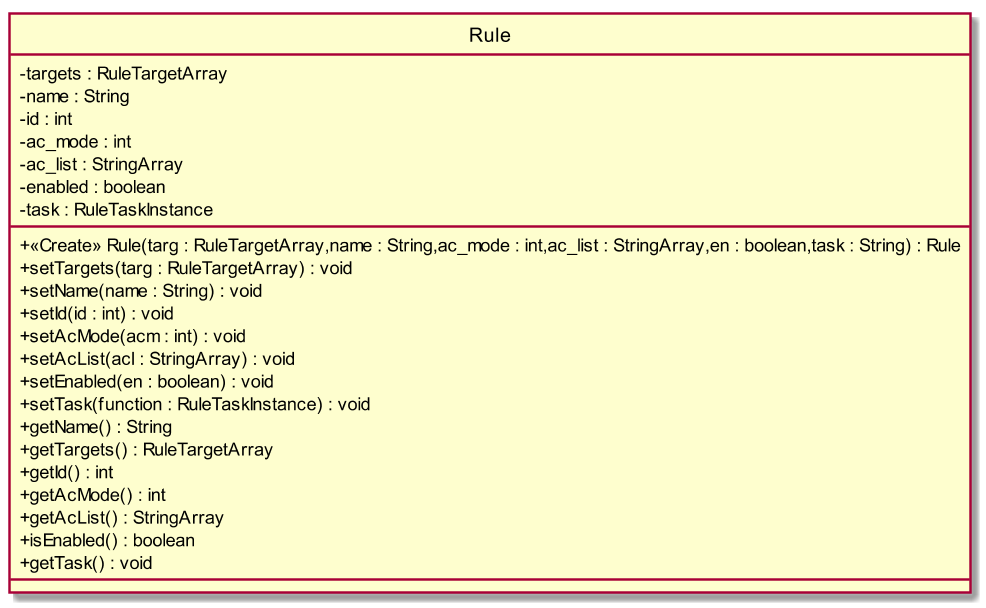
\includegraphics[width=\textwidth,height=\textheight,keepaspectratio]{images/ClassRule.png}
	\caption{Back-end::Rules::Rule}
\end{figure}
\begin{itemize}
	\item \textbf{Nome}: \file{Rule};
	\item \textbf{Tipo}: \file{Class};
	\item \textbf{Descrizione}: questa classe si occupa di rappresentare e organizzare i dati relativi ad una \file{Rule}, ovvero una direttiva definita da un amministratore;
	\item \textbf{Utilizzo}: fornisce i metodi getter e setter per i parametri relativi ad una direttiva, i quali dovranno essere memorizzati nel database per questo microservizio. Tramite il metodo \file{setTask}, è soggetta ad una setter-based dependency injection che ha come oggetto una \file{RuleTaskInstance}. \\
È utilizzata dalla classe \file{RulesDAO} e dalle classi che utilizzano quest'ultima;
	\item \textbf{Attributi}:
	\begin{itemize}
		\item[] \file{- targets: RuleTargetArray} \\
		Attributo contenente i targets della Rule;
		\item[] \file{- name: String} \\
		Attributo contenente il nome della Rule;
		\item[] \file{- id: int} \\
		Attributo contenente l'id della Rule;
		\item[] \file{- ac\_mode: int} \\
		Attributo contenente 0 per positivo, 1 per negativo;
		\item[] \file{- ac\_list: StringArray} \\
		Attributo contenente l'array di stringhe di id amministratori abilitati/disabilitati in base a valore di \file{ac\_mode};
		\item[] \file{- enabled: boolean} \\
		Attributo contenente un valore che dice se la Rule è abilitata o meno;
		\item[] \file{- task: RuleTaskInstance} \\
		Attributo contenente il compito della \file{Rule};
	\end{itemize}
	\item \textbf{Metodi}:
	\begin{itemize}
		\item[] \file{+ <<Create>> Rule(targ: RuleTargetArray, name: String, ac\_mode: int, ac\_list: StringArray, en: boolean, task: String): Rule} \\
		Metodo che permette di instanziare un oggetto \file{Rule} a partire da un nome, una lista dei targets un \file{ac\_mode}, un \file{ac\_list}, un compito da applicare e un valore booleano per abilitarla o meno;\\
		Parametri:
		\begin{itemize}
			\item \file{targ: RuleTargetArray} \\
			Parametro contenente l'array dei targets da assegnare alla Rule;
			\item \file{name: String} \\
			Parametro contenente il nome da assegnare alla Rule;
			\item \file{ac\_mode: int} \\
			Parametro contenente l'ac\_mode da assegnare alla Rule;
			\item \file{ac\_list: StringArray} \\
			Parametro contenente l'array di id degli amministratori abilitati/disabilitati da assegnare alla Rule;
			\item \file{en: boolean} \\
			Parametro contenente il valore booleano da assegnare alla Rule per abilitarla o meno;
			\item \file{task: String} \\
			Parametro contenente il compito da assegnare alla Rule;
		\end{itemize}
		\item[] \file{+ setTargets(targ: RuleTargetArray): void} \\
		Metodo che permette di passare un Array contenente i targets per la \file{Rule};\\
		Parametri:
		\begin{itemize}
			\item \file{targ: RuleTargetArray} \\
			Parametro contenente l'array dei targets da passare;
		\end{itemize}
		\item[] \file{+ setName(name: String): void} \\
		Metodo che permette di passare il nome per la \file{Rule};\\
		Parametri:
		\begin{itemize}
			\item \file{name: String} \\
			Parametro contenente il nome della Rule da passare;
		\end{itemize}
		\item[] \file{+ setId(id: int): void} \\
		Metodo che permette di passare l'id per la \file{Rule};\\
		Parametri:
		\begin{itemize}
			\item \file{id: int} \\
			Parametro contenente l'id da passare;
		\end{itemize}
		\item[] \file{+ setAcMode(acm: int): void} \\
		Metodo che permette di passare l'\file{ac\_mode} per la \file{Rule};\\
		Parametri:
		\begin{itemize}
			\item \file{acm: int} \\
			Parametro contenente l'ac\_mode da passare;
		\end{itemize}
		\item[] \file{+ setAcList(acl: StringArray): void} \\
		Metodo che permette di passare gli id degli amministratori abilitati/disabilitati per la \file{Rule};\\
		Parametri:
		\begin{itemize}
			\item \file{acl: StringArray} \\
			Parametro contenente l'ac\_list da passare;
		\end{itemize}
		\item[] \file{+ setEnabled(en: boolean): void} \\
		Metodo che permette di passare un valore da impostare ad \file{enabled} per la \file{Rule};\\
		Parametri:
		\begin{itemize}
			\item \file{en: boolean} \\
			Parametro contenente il valore booleano da passare;
		\end{itemize}
		\item[] \file{+ setTarget(function: RuleTaskInstance): void} \\
		Metodo che permette di passare il compito da applicare per la \file{Rule};\\
		Parametri:
		\begin{itemize}
			\item \file{function: RuleTaskInstance} \\
			Parametro contenente la function da passare;
		\end{itemize}
		\item[] \file{+ getName(): String} \\
		Metodo che permette di ottenere il nome della \file{Rule};\\
		\item[] \file{+ getTargets(): RuleTargetArray} \\
		Metodo che permette di ottenere l'array contenente i targets della \file{Rule};\\
		\item[] \file{+ getId(): int} \\
		Metodo che permette di ottenere l'id della \file{Rule};\\
		\item[] \file{+ getAcMode(): int} \\
		Metodo che permette di ottenere l'\file{ac\_mode} della \file{Rule};\\
		\item[] \file{+ getAcList(): StringArray} \\
		Metodo che permette di ottenere la lista degli id degli amministratori abilitati/disabilitati della \file{Rule};\\
		\item[] \file{+ isEnabled(): boolean} \\
		Metodo che permette di capire se la \file{Rule} è abilitata o meno;\\
		\item[] \file{+ getTask(): void} \\
		Metodo che permette di ottenere la \file{Task} applicata dalla \file{Rule};\\
	\end{itemize}
\end{itemize}

\hypertarget{RulesDAODynamoDB_label}{\paragraph{RulesDAODynamoDB}}
\begin{figure}[h]
	\centering
	\includegraphics[width=\textwidth,height=\textheight,keepaspectratio]{images/ClassRulesDAODynamoDB.png}
	\caption{Back-end::Rules::RulesDAODynamoDB}
\end{figure}
\begin{itemize}
	\item \textbf{Nome}: \file{RulesDAODynamoDB};
	\item \textbf{Tipo}: \file{Class};
	\item \textbf{Descrizione}: classe che si occupa di implementare l'interfaccia \file{RulesDAO}, utilizzando un database DynamoDB come supporto per la memorizzazione dei dati;
	\item \textbf{Utilizzo}: implementa i metodi dell'interfaccia \file{RulesDAO} interrogando un database DynamoDB. Utilizza \file{AWS::DynamoDB::DocumentClient} per l'accesso al database. La dependency injection dell'oggetto \file{AWS::DynamoDB} viene fatta utilizzando il costruttore;
	\item \textbf{Attributi}:
	\begin{itemize}
		\item[] \file{- db: AWS::DynamoDB} \\
		Attributo contenente un riferimento al modulo di Node.js utilizzato per l'accesso al database DynamoDB contenente la tabella degli utenti;
	\end{itemize}
	\item \textbf{Metodi}:
	\begin{itemize}
		\item[] \file{+ addRule(rule: Rule): ErrorObservable} \\
		Implementazione del metodo definito nell'interfaccia \file{RulesDAO}. Utilizza il metodo put del \file{DocumentClient} per aggiungere la Rule al database;\\
		Parametri:
		\begin{itemize}
			\item \file{rule: Rule} \\
			Parametro contenente la Rule da aggiungere;
		\end{itemize}
		\item[] \file{+ getRule(id: String): RuleObservable} \\
		Implementazione del metodo definito nell'interfaccia \file{RulesDAO}. Utilizza il metodo get del \file{DocumentClient} per ottenere i dati relativi ad uno \file{Rule} dal database;\\
		Parametri:
		\begin{itemize}
			\item \file{id: String} \\
			Parametro contenente l'id della Rule da recuperare;
		\end{itemize}
		\item[] \file{+ getRuleList(): RuleObservable} \\
		Implementazione del metodo dell'interfaccia \file{RulesDAO}. Utilizza il metodo scan del \file{DocumentClient} per ottenere la lista delle Rule dal database;\\
		\item[] \file{+ removeRule(id: String): ErrorObservable} \\
		Implementazione del metodo dell'interfaccia \file{RulesDAO}. Utilizza il metodo delete del \file{DocumentClient} per eliminare una Rule dal database;\\
		Parametri:
		\begin{itemize}
			\item \file{id: String} \\
			Parametro contenente l'id della Rule;
		\end{itemize}
		\item[] \file{+ updateRule(rule: Rule): ErrorObservable} \\
		Implementazione del metodo dell'interfaccia \file{RulesDAO}. Utilizza il metodo update del \file{DocumentClient} per aggiornare i dati relativi ad una Rule presente all'interno del database;\\
		Parametri:
		\begin{itemize}
			\item \file{rule: Rule} \\
			Parametro contenente la Rule da aggiornare;
		\end{itemize}
		\item[] \file{+ <> createRulesDAODynamoDB(db: AWS::DynamoDB): RulesDAODynamoDB} \\
		Constructor della classe \file{RulesDAODynamoDB}. Permette di effettuare la dependency injection di \file{AWS::DynamoDB};\\
		Parametri:
		\begin{itemize}
			\item \file{db: AWS::DynamoDB} \\
			Parametro contenente un riferimento al modulo di Node.js da utilizzare per l'accesso al database DynamoDB contenente la tabella delle rule;
		\end{itemize}
	\end{itemize}
\end{itemize}

\hypertarget{RulesService_label}{\paragraph{RulesService}}
\begin{figure}[h]
	\centering
	\includegraphics[width=\textwidth,height=\textheight,keepaspectratio]{images/ClassRulesService.png}
	\caption{Back-end::Rules::RulesService}
\end{figure}
\begin{itemize}
	\item \textbf{Nome}: \file{RulesService};
	\item \textbf{Tipo}: \file{Class};
	\item \textbf{Descrizione}: questa classe si occupa di realizzare il microservizio \file{Rules} e di interagire con il database delle direttive;
	\item \textbf{Utilizzo}: fornisce i metodi che implementano le lambda function necessarie alla gestione delle \file{Rule} e relative \file{Task}. Questa classe non interagisce direttamente con il database, ma fa utilizzo di \file{TasksDAO} e \file{RulesDAO}, le quali nascondono i meccanismi di accesso e persistenza dei dati nel database;
	\item \textbf{Attributi}:
	\begin{itemize}
		\item[] \file{- rules: RulesDAO} \\
		Attributo che permette di contattare il \file{RulesDAO}, il quale permette l'accesso al database delle \file{Rule};
		\item[] \file{- task: TasksDAO} \\
		Attributo che permette di contattare il \file{TasksDAO}, il quale permette di accedere al database delle \file{Task};
	\end{itemize}
	\item \textbf{Metodi}:
	\begin{itemize}
		\item[] \file{+ addRule(event: LambdaEvent, context: LambdaContext): void} \\
		Metodo che implementa la lambda function che si occupa di aggiungere una \file{Rule};\\
		Parametri:
		\begin{itemize}
			\item \file{event: LambdaEvent} \\
			Parametro contenente, all'interno del campo body sotto forma di stringa in formato JSON, un oggetto \file{Rule} contenente tutti i dati relativi ad una Rule da inserire;
			\item \file{context: LambdaContext} \\
			Parametro utilizzato dalle lambda function per inviare la risposta. Il \file{body} del \file{LambdaResponse}, parametro del metodo \file{LambdaContext::succeed}, conterrà una stringa vuota e il risultato di questa operazione sarà deducibile dal valore dell'attributo di \file{LambaResponse::statusCode};
		\end{itemize}
		\item[] \file{+ deleteRule(event: LambdaIdEvent, context: LambdaContext): void} \\
		Metodo che implementa la lambda function che si occupa di eliminare una \file{Rule};\\
		Parametri:
		\begin{itemize}
			\item \file{event: LambdaIdEvent} \\
			Parametro contenente, all'interno del campo \file{pathParameters}, l'identificativo della \file{Rule} che si vuole eliminare;
			\item \file{context: LambdaContext} \\
			Parametro utilizzato dalle lambda function per inviare la risposta. Il \file{body} del \file{LambdaResponse}, ottenuto dal metodo \file{LambdaContext::succeed}, conterrà una stringa vuota e il risultato di questa operazione sarà deducibile dal valore dell'attributo \file{LambdaResponse::statusCode};
		\end{itemize}
		\item[] \file{+ updateRule(event: LambdaIdEvent, context: LambdaContext): void} \\
		Metodo che implementa la lambda function che si occupa di aggiornare una \file{Rule};\\
		Parametri:
		\begin{itemize}
			\item \file{event: LambdaIdEvent} \\
			Parametro contenente all'interno del campo \file{body}, sotto forma di stringa in formato JSON, un oggetto di tipo \file{Rule} contente i dati da aggiornare e, all'interno del campo \file{pathParameters}, l'identificativo della \file{Rule} da modificare;
			\item \file{context: LambdaContext} \\
			Parametro utilizzato dalle lambda function per inviare la risposta. Il \file{body} del \file{LambdaResponse}, ottenuto dal metodo \file{LambdaContext::succeed}, conterrà una stringa vuota e il risultato di questa operazione sarà deducibile dal valore dell'attributo \file{LambaResponse::statusCode};
		\end{itemize}
		\item[] \file{+ getRule(event: LambdaIdEvent, context: LambdaContext): void} \\
		Metodo che implementa la lambda function che si occupa di ottenere una \file{Rule};\\
		Parametri:
		\begin{itemize}
			\item \file{event: LambdaIdEvent} \\
			Parametro contenente, all'interno del campo pathParameters, l'identificativo della \file{Rule} della quale si vogliono ottenere i dati;
			\item \file{context: LambdaContext} \\
			Parametro utilizzato dalle lambda function per inviare la risposta. Il \file{body} del \file{LambdaResponse}, ottenuto dal metodo \file{LambdaContext::succeed}, conterrà, sotto forma di stringa in formato JSON, un oggetto di tipo \file{Rule}, contenente i dati relativi alla \file{Rule} ritornata;
		\end{itemize}
		\item[] \file{+ getRuleList(event: LambdaEvent, context: LambdaContext): void} \\
		Metodo che implementa la lambda function che si occupa di ottenere l'array delle \file{Rule};\\
		Parametri:
		\begin{itemize}
			\item \file{event: LambdaEvent} \\
			Parametro contenente, all'interno del campo body, una stringa vuota;
			\item \file{context: LambdaContext} \\
			Parametro utilizzato dalle lambda function per inviare la risposta. Il \file{body} del \file{LambdaResponse}, parametro del metodo \file{LambdaContext::succeed}, conterrà, sotto forma di una stringa in formato JSON,  l'array delle \file{Rule} disponibili;
		\end{itemize}
		\item[] \file{+ getTaskList(event: LambdaEvent, context: LambdaContext): void} \\
		Metodo che implementa la lambda function che si occupa ottenere l'array delle \file{Task} disponibili;\\
		Parametri:
		\begin{itemize}
			\item \file{event: LambdaEvent} \\
			Parametro contenente, all'interno del campo body, una stringa vuota;
			\item \file{context: LambdaContext} \\
			Parametro utilizzato dalle lambda function per inviare la risposta. Il \file{body} del \file{LambdaResponse}, ottenuto dal metodo \file{LambdaContext::succeed}, conterrà, sotto forma di una stringa in formato JSON,  un Array di oggetti di tipo \file{Function};
		\end{itemize}
		\item[] \file{+ getTask(event: LambdaIdEvent, context: LambdaContext): void} \\
		Metodo che implementa la lambda function che si occupa di ottenere una \file{Task};\\
		Parametri:
		\begin{itemize}
			\item \file{event: LambdaIdEvent} \\
			Parametro contenente, all'interno del campo \file{pathParameters}, l'identificativo della \file{Rule} della quale si vuole ottenere la \file{Task};
			\item \file{context: LambdaContext} \\
			Parametro utilizzato dalle lambda function per inviare la risposta. Il \file{body} del \file{LambdaResponse}, parametro del metodo \file{LambdaContext::succeed}, conterrà, sotto forma di una stringa in formato JSON, un oggetto di tipo \file{RuleTaskInstance}, contenente i dati relativi alla \file{Task} ritornata;
		\end{itemize}
		\item[] \file{+ <<Create>> createRulesService(task: TasksDAO, rules: RulesDAO): RulesService} \\
		Metodo che permette di creare un \file{RulesService}. Permette la dependency injection avente come oggetti un \file{RulesDAO} e \file{TasksDAO};\\
		Parametri:
		\begin{itemize}
			\item \file{task: TasksDAO} \\
			Attributo contenente il \file{TasksDAO};
			\item \file{rules: RulesDAO} \\
			Attributo contenente il \file{RulesDAO};
		\end{itemize}
	\end{itemize}
\end{itemize}

\hypertarget{RuleTarget_label}{\paragraph{RuleTarget}}
\begin{figure}[h]
	\centering
	\includegraphics[width=\textwidth,height=\textheight,keepaspectratio]{images/ClassRuleTarget.png}
	\caption{Back-end::Rules::RuleTarget}
\end{figure}
\begin{itemize}
	\item \textbf{Nome}: \file{RuleTarget};
	\item \textbf{Tipo}: \file{Class};
	\item \textbf{Descrizione}: questa classe si occupa di rappresentare e organizzare i dati relativi a un target di una \file{Rule}, ovvero la persona alla quale è indirizzata quest'ultima;
	\item \textbf{Utilizzo}: fornisce gli attributi di un target di una \file{Rule} che dovranno essere memorizzati nel database per questo microservizio.
Viene utilizzata dalla classe \file{Rule} per definire un Array di \file{Target} ai quali applicare la sua funzione;
	\item \textbf{Attributi}:
	\begin{itemize}
		\item[] \file{+ company: String} \\
		Attributo contenente il nome dell'azienda;
		\item[] \file{+ name: String} \\
		Attributo contenente il nome del target;
		\item[] \file{+ member: String} \\
		Attributo contenente ??? perchè un target dovrebbe contenenre il nome di uno di zero12?;
	\end{itemize}
\end{itemize}

\hypertarget{RuleTaskInstance_label}{\paragraph{RuleTaskInstance}}
\begin{figure}[h]
	\centering
	\includegraphics[width=\textwidth,height=\textheight,keepaspectratio]{images/ClassRuleTaskInstance.png}
	\caption{Back-end::Rules::RuleTaskInstance}
\end{figure}
\begin{itemize}
	\item \textbf{Nome}: \file{RuleTaskInstance};
	\item \textbf{Tipo}: \file{Class};
	\item \textbf{Descrizione}: questa classe si occupa di rappresentare i dati relativi al compito di una direttiva;
	\item \textbf{Utilizzo}: fornisce un meccanismo per specificare la modifica di comportamento del sistema in seguito all'applicazione di una determinata direttiva. ;
	\item \textbf{Attributi}:
	\begin{itemize}
		\item[] \file{+ task: String} \\
		Attributo contenente il task, ovvero una funzione, da applicare;
		\item[] \file{+ params: Array} \\
		Attributo contenente l'array dei parametri relativi alla funzione;
	\end{itemize}
\end{itemize}

\hypertarget{Task_label}{\paragraph{Task}}
\begin{figure}[h]
	\centering
	\includegraphics[width=\textwidth,height=\textheight,keepaspectratio]{images/ClassTask.png}
	\caption{Back-end::Rules::Task}
\end{figure}
\begin{itemize}
	\item \textbf{Nome}: \file{Task};
	\item \textbf{Tipo}: \file{Class};
	\item \textbf{Descrizione}: questa classe si occupa di rappresentare la funzione che dovrà essere applicata ad una \file{Rule};
	\item \textbf{Utilizzo}: fornisce gli attributi delle funzioni (ovvero dei compiti che una certa \file{Rule} svolge) che dovranno essere applicate a certe \file{Rule}, i quali dovranno essere memorizzati nel database per questo microservizio;
	\item \textbf{Attributi}:
	\begin{itemize}
		\item[] \file{+ function: String} \\
		Attributo contenente la funzione da applicare;
		\item[] \file{+ id: int} \\
		Attributo contenente l'id della funzione;
	\end{itemize}
\end{itemize}

\hypertarget{TasksDAODynamoDB_label}{\paragraph{TasksDAODynamoDB}}
\begin{figure}[h]
	\centering
	\includegraphics[width=\textwidth,height=\textheight,keepaspectratio]{images/ClassTasksDAODynamoDB.png}
	\caption{Back-end::Rules::TasksDAODynamoDB}
\end{figure}
\begin{itemize}
	\item \textbf{Nome}: \file{TasksDAODynamoDB};
	\item \textbf{Tipo}: \file{Class};
	\item \textbf{Descrizione}: classe che si occupa di implementare l'interfaccia \file{TasksDAO}, utilizzando un database DynamoDB come supporto per la memorizzazione dei dati;
	\item \textbf{Utilizzo}: implementa i metodi dell'interfaccia \file{TasksDAO} interrogando un database DynamoDB. Utilizza \file{AWS::DynamoDB::DocumentClient} per l'accesso al database. La dependency injection dell'oggetto \file{AWS::DynamoDB} viene fatta utilizzando il costruttore;
	\item \textbf{Attributi}:
	\begin{itemize}
		\item[] \file{- db: AWS::DynamoDB} \\
		Attributo contenente un riferimento al modulo di Node.js utilizzato per l'accesso al database DynamoDB contenente la tabella degli utenti;
	\end{itemize}
	\item \textbf{Metodi}:
	\begin{itemize}
		\item[] \file{+ addFunction(fun: Function): ErrorObservable} \\
		Implementazione del metodo definito nell'interfaccia \file{FunctionsDAO}. Utilizza il metodo put del \file{DocumentClient} per aggiungere la funzione al database;\\
		Parametri:
		\begin{itemize}
			\item \file{fun: Function} \\
			Parametro contenente la funzione;
		\end{itemize}
		\item[] \file{+ getFunction(id: String): TaskObservable} \\
		Implementazione del metodo definito nell'interfaccia \file{FunctionsDAO}. Utilizza il metodo get del \file{DocumentClient} per ottenere i dati relativi ad una \file{Function} dal database;\\
		Parametri:
		\begin{itemize}
			\item \file{id: String} \\
			Parametro contenente l'id della funzione;
		\end{itemize}
		\item[] \file{+ getFunctionList(): TaskObservable} \\
		Implementazione del metodo dell'interfaccia \file{FunctionsDAO}. Utilizza il metodo scan del \file{DocumentClient} per ottenere la lista delle funzioni dal database;\\
		\item[] \file{+ removeFunction(id: String): ErrorObservable} \\
		Implementazione del metodo dell'interfaccia \file{FunctionsDAO}. Utilizza il metodo delete del \file{DocumentClient} per eliminare una funzione dal database;\\
		Parametri:
		\begin{itemize}
			\item \file{id: String} \\
			Parametro contenente l'id della funzione;
		\end{itemize}
		\item[] \file{+ updateFunction(fun: Function): ErrorObservable} \\
		Implementazione del metodo dell'interfaccia \file{FunctionsDAO}. Utilizza il metodo update del \file{DocumentClient} per aggiornare i dati relativi ad una funzione presente all'interno del database;\\
		Parametri:
		\begin{itemize}
			\item \file{fun: Function} \\
			Parametro contenente la funzione;
		\end{itemize}
		\item[] \file{+ <> createFunctionsDAODynamoDB(db: AWS::DynamoDB): TasksDAODynamoDB} \\
		Constructor della classe \file{FunctionsDAODynamoDB}. Permette di effettuare la dependency injection di \file{AWS::DynamoDB};\\
		Parametri:
		\begin{itemize}
			\item \file{db: AWS::DynamoDB} \\
			Parametro contenente un riferimento al modulo di Node.js da utilizzare per l'accesso al database DynamoDB contenente la tabella delle funzioni;
		\end{itemize}
	\end{itemize}
\end{itemize}

\subsection{Back-end::STT}
Package che include le classi che si occupano di fornire le funzionalità di Speech to text.
\subsubsection{Classi}
\hypertarget{ STTModule_label}{\paragraph{ STTModule}}
\begin{figure}[h]
	\centering
	\includegraphics[width=\textwidth,height=\textheight,keepaspectratio]{images/Class STTModule.png}
	\caption{Back-end::STT:: STTModule}
\end{figure}
\begin{itemize}
	\item \textbf{Nome}: \file{ STTModule};
	\item \textbf{Tipo}: \file{Interface};
	\item \textbf{Descrizione}: classe che definisce l'interfaccia dei moduli utilizzati per le operazioni di Speech-To-Text (STT);
	\item \textbf{Utilizzo}: fornisce l'interfaccia che deve essere implementata dai moduli che permettono l'accesso alle funzionalità di STT;
	\item \textbf{Metodi}:
	\begin{itemize}
		\item[] \file{+ speechToText(audio: Buffer, type: String): StringPromise} \\
		Questo metodo permette di ricavare in modo asincrono il testo da un file audio. Viene utilizzato da \file{VirtualAssistantAPI}, il quale invierà il testo ottenuto dall'invocazione di questo metodo all'assistente virtuale. Restituisce una promise che verrà soddisfatta con una stringa contenente il testo estratto;\\
		Parametri:
		\begin{itemize}
			\item \file{audio: Buffer} \\
			Buffer contenente l'audio da cui si vuole estrarre il testo;
			\item \file{type: String} \\
			Parametro contenete la descrizione del formato in cui i dati sono memorizzati in \file{audio};
		\end{itemize}
	\end{itemize}
\end{itemize}

\hypertarget{STTWatsonAdapter_label}{\paragraph{STTWatsonAdapter}}
\begin{figure}[h]
	\centering
	\includegraphics[width=\textwidth,height=\textheight,keepaspectratio]{images/ClassSTTWatsonAdapter.png}
	\caption{Back-end::STT::STTWatsonAdapter}
\end{figure}
\begin{itemize}
	\item \textbf{Nome}: \file{STTWatsonAdapter};
	\item \textbf{Tipo}: \file{Class};
	\item \textbf{Descrizione}: questa classe si occupa di convertire l'interfaccia fornita dal servizio di Speech to Text di IBM in una più adatta alle esigenze dell'applicazione, definita da \file{STTModule}. \\
Facendo da Adapter tra le API del servizio di Speech to Text di IBM (adaptee) e l'interfaccia \file{STTModule} (target) utilizzata da \file{APIGateway::VocalAPI}, permette l'interoperabilità tra queste due interfacce;
	\item \textbf{Utilizzo}:
Fornisce a \file{STTModule} un meccanismo che permette di interrogare le API del servizio Watson Speech to Text di IBM, in modo da consentire a \file{APIGateway::VocalAPI} l'utilizzo di quest'ultime utilizzando un'interfaccia distinta e più consona alle proprie esigenze. \\ È soggetta ad una constructor-based dependency injection, la quale ha come oggetti:
\begin{itemize}
   \item uno \file{StreamBufferModule} contenente ... ??? ;
   \item uno \file{SpeechToTextV1} ???
\end{itemize}
Per ulteriori informazioni, consultare le documentazioni presenti alle seguenti pagine:
\begin{itemize}
    \item \url{https://www.ibm.com/watson/developercloud/doc/speech-to-text/};
    \item \url{https://github.com/watson-developer-cloud/node-sdk#speech-to-text}.
\end{itemize};
	\item \textbf{Attributi}:
	\begin{itemize}
		\item[] \file{- stt: SpeechToTextV1} \\
		Attributo contenente il \file{SpeechToTextV1Module}, creato a partire dai parametri \file{name} e \file{password} forniti al costruttore. Viene utilizzato per estrarre il contenuto testuale di un file audio utilizzando il servizio Watson Speech To Text di IBM;
		\item[] \file{- stream\_buffer: StreamBufferModule} \\
		Attributo contenente il \file{StreamBufferModule} di cui è stata effettuate la dependency injection nel costruttore. Viene utilizzata per creare un \file{ReadableStream} di node a partire da un buffer;
	\end{itemize}
	\item \textbf{Metodi}:
	\begin{itemize}
		\item[] \file{+ <<Create>> createSTTWatsonAdapter(sb: StreamBufferModule, stt: SpeechToTextV1): STTWatsonAdapter} \\
		Costruttore di STTWatsonAdapter, che permette di effettuare la dependency injection di \file{StreamBufferModule} e di \file{SpeechToTextV1};\\
		Parametri:
		\begin{itemize}
			\item \file{sb: StreamBufferModule} \\
			Parametro tramite i quale si effettua la dependency injection di \file{StreamBufferModule};
			\item \file{stt: SpeechToTextV1} \\
			Parametro tramite il quale viene effettuata la dependency injection di \file{SpeechToTextV1}. ;
		\end{itemize}
		\item[] \file{+ speechToText(audio: Buffer, type: String): StringPromise} \\
			Implementa il metodo \file{speechToText} contenuto nell'interfaccia;\\
		Parametri:
		\begin{itemize}
			\item \file{audio: Buffer} \\
			Parametro contenente l'audio dal quale si vuole estrarre il testo;
			\item \file{type: String} \\
			Parametro contenente il formato in cui sono memorizzati i dati all'interno di \file{audio};
		\end{itemize}
	\end{itemize}
\end{itemize}

\subsection{Back-end::Utility}
Package contenente classi e interfacce, dallo scopo generico, utili ad altri package del back-end.
\subsubsection{Classi}
\hypertarget{Error_label}{\paragraph{Error}}
\begin{figure}[h]
	\centering
	\includegraphics[width=\textwidth,height=\textheight,keepaspectratio]{images/ClassError.png}
	\caption{Back-end::Utility::Error}
\end{figure}
\begin{itemize}
	\item \textbf{Nome}: \file{Error};
	\item \textbf{Tipo}: \file{Class};
	\item \textbf{Descrizione}: questa classe si occupa di rappresentare e organizzare i dati relativi ad un errore che può avvenire;
	\item \textbf{Utilizzo}: fornisce gli attributi necessari a descrivere gli errori che si possono verificare.
L'attributo \file{code} contiene un valore uguale a 0 nel caso non si sia verificato nessun errore, diverso da 0 altrimenti.
Nel caso di \file{code} diverso da 0, l'attributo \file{msg} contiene una stringa che descrive l'errore verificatosi;
	\item \textbf{Attributi}:
	\begin{itemize}
		\item[] \file{+ code: String} \\
		Attributo contenente il codice dell'errore;
		\item[] \file{+ msg: String[0..1]} \\
		Attributo contenente il messaggio dell'errore;
	\end{itemize}
\end{itemize}

\hypertarget{LambdaContext_label}{\paragraph{LambdaContext}}
\begin{figure}[h]
	\centering
	\includegraphics[width=\textwidth,height=\textheight,keepaspectratio]{images/ClassLambdaContext.png}
	\caption{Back-end::Utility::LambdaContext}
\end{figure}
\begin{itemize}
	\item \textbf{Nome}: \file{LambdaContext};
	\item \textbf{Tipo}: \file{Class};
	\item \textbf{Descrizione}: questa classe si occupa di rappresentare un oggetto context passato alle lambda function;
	\item \textbf{Utilizzo}: fornisce un metodo che permette di inviare una risposta all'API Gateway. ;
	\item \textbf{Metodi}:
	\begin{itemize}
		\item[] \file{+ succeed(res: LambdaResponse): void} \\
		Metodo che permette di inviare una risposta all'API Gateway;\\
		Parametri:
		\begin{itemize}
			\item \file{res: LambdaResponse} \\
			Attributo contenente la risposta da inviare;
		\end{itemize}
		\item[] \file{+ getRemainingTimeInMillis(): int} \\
		DA TOGLIERE DA TOGLIERE DA TOGLIERE DA TOGLIEREDA TOGLIERE DA TOGLIEREDA TOGLIERE DA TOGLIEREDA TOGLIERE DA TOGLIEREDA TOGLIERE DA TOGLIEREDA TOGLIERE DA TOGLIEREDA TOGLIERE DA TOGLIEREDA TOGLIERE DA TOGLIEREDA TOGLIERE DA TOGLIEREDA TOGLIERE DA TOGLIEREDA TOGLIERE DA TOGLIEREDA TOGLIERE DA TOGLIERE;\\
	\end{itemize}
\end{itemize}

\hypertarget{LambdaEvent_label}{\paragraph{LambdaEvent}}
\begin{figure}[h]
	\centering
	\includegraphics[width=\textwidth,height=\textheight,keepaspectratio]{images/ClassLambdaEvent.png}
	\caption{Back-end::Utility::LambdaEvent}
\end{figure}
\begin{itemize}
	\item \textbf{Nome}: \file{LambdaEvent};
	\item \textbf{Tipo}: \file{Class};
	\item \textbf{Descrizione}: classe che rappresenta l'oggetto event che viene passato alle LambdaFuction dall'API Gateway con l'integrazione Lambda Proxy;
	\item \textbf{Utilizzo}: fornisce i parametri necessari alla lambda function per gestire le richieste che arrivano all'API Gateway;
	\item \textbf{Figlio}: \file{LambdaIdEvent};
	\item \textbf{Attributi}:
	\begin{itemize}
		\item[] \file{+ body: String} \\
		Stringa contente i dati ricevuti dall'API Gateway. Le singole Lambda  Function si dovranno occupare dell'interpretazione di tale stringa nel formato adeguato (ad esempio JSON, testo, ecc.);
		\item[] \file{+ headers: StringAssocArray} \\
		Array associativo di stringhe contenente gli headers HTTP della richiesta ricevuta dall'API Gateway;
	\end{itemize}
\end{itemize}

\hypertarget{LambdaIdEvent_label}{\paragraph{LambdaIdEvent}}
\begin{figure}[h]
	\centering
	\includegraphics[width=\textwidth,height=\textheight,keepaspectratio]{images/ClassLambdaIdEvent.png}
	\caption{Back-end::Utility::LambdaIdEvent}
\end{figure}
\begin{itemize}
	\item \textbf{Nome}: \file{LambdaIdEvent};
	\item \textbf{Tipo}: \file{Class};
	\item \textbf{Descrizione}: classe che rappresenta un oggetto event che viene passato alle Lambda function dall'API Gateway con l'integrazione Lambda Proxy;
	\item \textbf{Utilizzo}: eredita da LambdaEvent ed aggiunge l'attributo pathParameters;
	\item \textbf{Padre}: \file{LambdaEvent};
	\item \textbf{Attributi}:
	\begin{itemize}
		\item[] \file{+ pathParameters: PathIdParam} \\
		Parametro contenente l'id dell'utente del quale si vogliono ottenere i dati;
	\end{itemize}
\end{itemize}

\hypertarget{LambdaResponse_label}{\paragraph{LambdaResponse}}
\begin{figure}[h]
	\centering
	\includegraphics[width=\textwidth,height=\textheight,keepaspectratio]{images/ClassLambdaResponse.png}
	\caption{Back-end::Utility::LambdaResponse}
\end{figure}
\begin{itemize}
	\item \textbf{Nome}: \file{LambdaResponse};
	\item \textbf{Tipo}: \file{Class};
	\item \textbf{Descrizione}: questa classe si occupa di rappresentare la risposta di una lambda function;
	\item \textbf{Utilizzo}: fornisce alle lambda function gli attributi necessari per inviare una risposta ad API Gateway;
	\item \textbf{Attributi}:
	\begin{itemize}
		\item[] \file{+ statusCode: int} \\
		Attributo contenente il codice di stato HTTP che dovrà avere la risposta;
		\item[] \file{+ headers: StringAssocArray} \\
		Attributo contenente l'array associativo nel quale la chiave indica il nome di un header HTTP da mandare nella risposta ed il valore è una stringa contenente il valore di tale header;
		\item[] \file{+ body: String} \\
		Attributo contenente il corpo della risposta;
	\end{itemize}
\end{itemize}

\hypertarget{PathIdParam_label}{\paragraph{PathIdParam}}
\begin{figure}[h]
	\centering
	\includegraphics[width=\textwidth,height=\textheight,keepaspectratio]{images/ClassPathIdParam.png}
	\caption{Back-end::Utility::PathIdParam}
\end{figure}
\begin{itemize}
	\item \textbf{Nome}: \file{PathIdParam};
	\item \textbf{Tipo}: \file{Class};
	\item \textbf{Descrizione}: questa classe rappresenta i parametri path di una richiesta caratterizzata da un unico parametro che è un identificativo;
	\item \textbf{Utilizzo}: fornisce l'attributo che contiene l'identificativo della risorsa richiesta;
	\item \textbf{Attributi}:
	\begin{itemize}
		\item[] \file{+ id: String} \\
		Attributo contenente l'id della risorsa richiesta;
	\end{itemize}
\end{itemize}

\hypertarget{ProcessingResult_label}{\paragraph{ProcessingResult}}
\begin{figure}[h]
	\centering
	\includegraphics[width=\textwidth,height=\textheight,keepaspectratio]{images/ClassProcessingResult.png}
	\caption{Back-end::Utility::ProcessingResult}
\end{figure}
\begin{itemize}
	\item \textbf{Nome}: \file{ProcessingResult};
	\item \textbf{Tipo}: \file{Class};
	\item \textbf{Descrizione}: questa classe si occupa di rappresentare il campo result della risposta fornita da api.ai;
	\item \textbf{Utilizzo}: fornisce gli attributi per rappresentare l'oggetto result relativo ad una risposta di api.ai. \\
Per la relativa documentazione, consultare la pagina \url{https://docs.api.ai/docs/query#response};
	\item \textbf{Attributi}:
	\begin{itemize}
		\item[] \file{+ source: String} \\
		Attributo contenente la sorgente dalla quale è stata ricavata la risposta. ;
		\item[] \file{+ resolvedQuery: String} \\
		Attributo contenente il testo dell'intents utilizzato per interrogare api.ai;
		\item[] \file{+ action: String} \\
		Attributo contenente l'azione da eseguire;
		\item[] \file{+ actionIncomplete: boolean} \\
		Attributo contenete un valore booleano che indica se i parametri necessari a far eseguire l'azione sono stati forniti tutti o meno. ;
		\item[] \file{+ parameters: StringAssocArray} \\
		Attributo contenente un oggetto costituito dai parametri necessari per portare a termine l'azione;
		\item[] \file{+ contexts: ContextArray} \\
		Attributo contenente l'array dei context attivi;
		\item[] \file{+ fulfilment: Fulfillment} \\
		Attributo contenente i dati ricevuti dal webhook;
		\item[] \file{+ score: Real} \\
		Attributo contenente un numero, contenuto nell'intervallo [0,1], che indica la sicurezza con  la quale è stato trovato il relativo intent;
		\item[] \file{+ metadata: Metadata} \\
		Attributo contenente dati relativi a intents e contexts;
	\end{itemize}
\end{itemize}

\hypertarget{StatusObject_label}{\paragraph{StatusObject}}
\begin{figure}[h]
	\centering
	\includegraphics[width=\textwidth,height=\textheight,keepaspectratio]{images/ClassStatusObject.png}
	\caption{Back-end::Utility::StatusObject}
\end{figure}
\begin{itemize}
	\item \textbf{Nome}: \file{StatusObject};
	\item \textbf{Tipo}: \file{Class};
	\item \textbf{Descrizione}: questa classe si occupa di rappresentare lo status object della richiesta mandata ad api.ai, che indica se quest'ultima ha avuto successo o meno.
;
	\item \textbf{Utilizzo}: fornisce gli attributi per rappresentare l'oggetto status object relativo ad una richiesta mandata ad api.ai. \\
Per la relativa documentazione, consultare la pagina \url{https://docs.api.ai/docs/status-object};
	\item \textbf{Attributi}:
	\begin{itemize}
		\item[] \file{+ code: int} \\
		Attributo contenente il codice di stato HTTP;
		\item[] \file{+ errorType: String} \\
		Attributo contenente una breve descrizione dell'errore verificatosi. In caso non se ne verifichino, questo attributo avrà valore pari a "success";
		\item[] \file{+ errorId: String} \\
		Attributo contenente l'id dell'errore verificatosi;
		\item[] \file{+ errorDetails: String} \\
		Attributo contenente la descrizione dettagliata dell'errore verificatosi. In caso non se ne verifichino, questo attributo non sarà ritornato;
	\end{itemize}
\end{itemize}

\subsection{Back-end::VirtualAssistant}
Package contenente le componenti del microservizio dell'assistente virtuale.
\subsubsection{Classi}
\hypertarget{ AgentsDAO_label}{\paragraph{ AgentsDAO}}
\begin{figure}[h]
	\centering
	\includegraphics[width=\textwidth,height=\textheight,keepaspectratio]{images/Class AgentsDAO.png}
	\caption{Back-end::VirtualAssistant:: AgentsDAO}
\end{figure}
\begin{itemize}
	\item \textbf{Nome}: \file{ AgentsDAO};
	\item \textbf{Tipo}: \file{Interface};
	\item \textbf{Descrizione}: questa classe si occupa di astrarre le modalità di accesso al database contenente gli \file{Agent} disponibili;
	\item \textbf{Utilizzo}: fornisce a \file{WebhookService} un meccanismo per accedere ai dati relativi agli \file{Agent}, senza conoscerne le modalità di implementazioni e di persistenza del database. A partire da un identificativo, permette operazioni di lettura, scrittura e rimozione degli \file{Agent};
	\item \textbf{Attributi}:
	\begin{itemize}
		\item[] \file{- db: AWS::DynamoDB} \\
		Da fare;
	\end{itemize}
	\item \textbf{Metodi}:
	\begin{itemize}
		\item[] \file{+ getAgentsList(): AgentObservable} \\
		L'\file{Observable} restituito manderà agli \file{Observer} gli agents ottenuti, uno alla volta, e poi chiama il loro metodo \file{complete}. Nel caso in cui si verifichi un errore, gli \file{Observer} iscritti verranno notificati tramite la chiamate del loro metodo \file{error} con i dati relativi all'errore verificatosi;\\
		\item[] \file{+ updateAgent(agent: Agent): ErrorObservable} \\
		Metodo che permette di aggiornare un \file{Agent}.  L'\file{Observable} restituito non riceverà alcun valore, ma verrà completato in caso di aggiornamento dell'\file{Agent} avvenuta con successo. In caso di errore durante l'aggiornamento dell'\file{Agent}, gli \file{Observer} interessati verranno notificati tramite la chiamata del loro metodo \file{error()} con i dati relativi all'errore verificatosi;\\
		Parametri:
		\begin{itemize}
			\item \file{agent: Agent} \\
			Parametro contenente l'agente da aggiornare;
		\end{itemize}
		\item[] \file{+ removeAgent(name: String): ErrorObservable} \\
		Metodo che permette di rimuovere un Agent a partire da un name.  L'\file{Observable} restituito non riceverà alcun valore, ma verrà completato in caso di rimozione dell'\file{Agent} avvenuta con successo. In caso di errore durante la rimozione dell'\file{Agent}, gli \file{Observer} interessati verranno notificati tramite la chiamata del loro metodo \file{error()} con i dati relativi all'errore verificatosi;\\
		Parametri:
		\begin{itemize}
			\item \file{name: String} \\
			Parametro contenente il name dell'agente da rimuovere;
		\end{itemize}
		\item[] \file{+ addAgent(agent: Agent): ErrorObservable} \\
		Metodo che permette di aggiungere un \file{Agent}.  L'\file{Observable} restituito non riceverà alcun valore, ma verrà completato in caso di aggiunta dell'\file{Agent} avvenuta con successo. In caso di errore durante l'aggiunta dell'\file{Agent}, gli \file{Observer} interessati verranno notificati tramite la chiamata del loro metodo \file{error()} con i dati relativi all'errore verificatosi;\\
		Parametri:
		\begin{itemize}
			\item \file{agent: Agent} \\
			Parametro contenente l'agente da aggiungere al database;
		\end{itemize}
		\item[] \file{+ getAgent(name: String): AgentObservable} \\
		Metodo che ritorna un Agent a partire da un name. L'\file{Observable} restituito riceverà l'oggetto rappresentante tale \file{Agent}, e verrà completato. Nel caso in cui l'\file{Agent} richiesto non sia presente nel database, gli \file{Observer} interessati non riceveranno alcun valore, ma verranno notificati tramite la chiamata del loro metodo \file{error()};\\
		Parametri:
		\begin{itemize}
			\item \file{name: String} \\
			Parametro contenente il name dell'agente da ricevere;
		\end{itemize}
	\end{itemize}
\end{itemize}

\hypertarget{ VAModule_label}{\paragraph{ VAModule}}
\begin{figure}[h]
	\centering
	\includegraphics[width=\textwidth,height=\textheight,keepaspectratio]{images/Class VAModule.png}
	\caption{Back-end::VirtualAssistant:: VAModule}
\end{figure}
\begin{itemize}
	\item \textbf{Nome}: \file{ VAModule};
	\item \textbf{Tipo}: \file{Interface};
	\item \textbf{Descrizione}: questa classe definisce l'interfaccia dei moduli che si occupano di interrogare le API di un assistente virtuale;
	\item \textbf{Utilizzo}: fornisce la definizione dei metodi che dovranno essere implementati, in maniera tale da permettere ad un modulo che si interfacci con api.ai di essere utilizzato da \file{VAService};
	\item \textbf{Figlio}: \file{ApiAiVAAdapter};
	\item \textbf{Metodi}:
	\begin{itemize}
		\item[] \file{+ query(str: VAQuery): VAResponse} \\
		Metodo che permette di interrogare l'assistente virtuale;\\
		Parametri:
		\begin{itemize}
			\item \file{str: VAQuery} \\
			Parametro contenente i dati necessari all'interrogazione dell'assistente virtuale;
		\end{itemize}
	\end{itemize}
\end{itemize}

\hypertarget{ WebhookService_label}{\paragraph{ WebhookService}}
\begin{figure}[h]
	\centering
	\includegraphics[width=\textwidth,height=\textheight,keepaspectratio]{images/Class WebhookService.png}
	\caption{Back-end::VirtualAssistant:: WebhookService}
\end{figure}
\begin{itemize}
	\item \textbf{Nome}: \file{ WebhookService};
	\item \textbf{Tipo}: \file{Interface};
	\item \textbf{Descrizione}: questa classe definisce l'interfaccia dei moduli che implementano dei webhook conformi alle specifiche di api.ai;
	\item \textbf{Utilizzo}: fornisce una serie di metodi necessari per definire un servizio che soddisfi i requisiti per webhook di api.ai.
Per la relativa documentazione, consultare la pagina \url{https://docs.api.ai/docs/webhook};
	\item \textbf{Figli}: \file{ConversationWebhookService}, \file{AdministrationWebhookService};
	\item \textbf{Metodi}:
	\begin{itemize}
		\item[] \file{+ webhook(event: LambaEvent, context: LambdaContext): void} \\
		Metodo che fornisce l'interfaccia di una lambda function compatibile con i requisiti per webhook di api.ai;\\
		Parametri:
		\begin{itemize}
			\item \file{event: LambaEvent} \\
			Parametro contenente i dati mandati da api.ai al WebhookService;
			\item \file{context: LambdaContext} \\
			Parametro utilizzato dalle lambda function per inviare la risposta dal \file{WebhookService} ad api.ai. Il \file{body} del \file{LambdaResponse}, parametro del metodo \file{LambdaContext::succeed}, conterrà un oggetto , sotto forma di stringa in formato JSON, contenente i dati relativi all'utente ritornato.\\
Tali dati sono cosi organizzati:
\begin{lstlisting}[language=json,firstnumber=1]
{
    "contextOut":"ContextArray",
    "data":"Object",
    "displayText":"String",
    "followupEvent":"Object",
    "source":"String",
    "speech":"String"
}
\end{lstlisting}
Dove:
\begin{itemize}
    \item \file{contextOut}: attributo contenente l'array dei context che la richiesta ha attivato;
    \item \file{data}: attributo contenente i dati che saranno inviati al client. Tali dati non sono processati da api.ai e quindi saranno nella forma originale;
    \item \file{displayText}: attributo contenente il testo che verrà mostrato sullo schermo dell'utente;
    \item \file{followupEvent}: attributo contenente parametri opzionali che il servizio web utilizzato vuole inviare ad api.ai;
    \item \file{source}: attributo contenente la risorse dei dati forniti come risposta;
    \item \file{speech}: attributo contenente la risposta testuale alla richiesta.
\end{itemize}

Per la relativa documentazione, consultare la pagina Per una descrizione dettagliata si rimanda alla pagina \url{https://docs.api.ai/docs/webhook#section-format-of-response-from-the-service}.
;
		\end{itemize}
	\end{itemize}
\end{itemize}

\hypertarget{Agent_label}{\paragraph{Agent}}
\begin{figure}[h]
	\centering
	\includegraphics[width=\textwidth,height=\textheight,keepaspectratio]{images/ClassAgent.png}
	\caption{Back-end::VirtualAssistant::Agent}
\end{figure}
\begin{itemize}
	\item \textbf{Nome}: \file{Agent};
	\item \textbf{Tipo}: \file{Class};
	\item \textbf{Descrizione}: questa classe si occupa di rappresentare e organizzare i dati relativi ad un Agent di api.ai;
	\item \textbf{Utilizzo}: fornisce gli attributi di un Agent che dovranno essere memorizzati nel database per questo microservizio.
In api.ai, un Agent ha lo scopo di trasformare il linguaggio naturale, ricevuto in input, in dati capibili per le applicazioni.
Per la relativa documentazione, consultare questa pagina \url{https://docs.api.ai/docs/concept-agents};
	\item \textbf{Attributi}:
	\begin{itemize}
		\item[] \file{+ name: String} \\
		Nome dell'applicazione a cui è collegato l'agent.
Per ogni applicazione, abbiamo un Agent;
		\item[] \file{+ token: String} \\
		Attributo contenente il valore del token associato. Un agent è identificabile tramite esso;
		\item[] \file{+ lang: String} \\
		Attributo contenente la lingua, la quale dovrà essere sempre inglese (en);
	\end{itemize}
\end{itemize}

\hypertarget{AgentsDAODynamoDB_label}{\paragraph{AgentsDAODynamoDB}}
\begin{figure}[h]
	\centering
	\includegraphics[width=\textwidth,height=\textheight,keepaspectratio]{images/ClassAgentsDAODynamoDB.png}
	\caption{Back-end::VirtualAssistant::AgentsDAODynamoDB}
\end{figure}
\begin{itemize}
	\item \textbf{Nome}: \file{AgentsDAODynamoDB};
	\item \textbf{Tipo}: \file{Class};
	\item \textbf{Descrizione}: classe che si occupa di implementare l'interfaccia \file{AgentsDAO}, utilizzando un database DynamoDB come supporto per la memorizzazione dei dati;
	\item \textbf{Utilizzo}: implementa i metodi dell'interfaccia \file{AgentsDAO} interrogando un database DynamoDB. Utilizza \file{AWS::DynamoDB::DocumentClient} per l'accesso al database. La dependency injection dell'oggetto \file{AWS::DynamoDB} viene fatta utilizzando il costruttore;
	\item \textbf{Attributi}:
	\begin{itemize}
		\item[] \file{- db: AWS::DynamoDB} \\
		Attributo contenente un riferimento al modulo di Node.js utilizzato per l'accesso al database DynamoDB contenente la tabella degli utenti;
	\end{itemize}
	\item \textbf{Metodi}:
	\begin{itemize}
		\item[] \file{+ addAgent(agent: Agent): ErrorObservable} \\
		Implementazione del metodo definito nell'interfaccia \file{AgentsDAO}. Utilizza il metodo put del \file{DocumentClient} per aggiungere l'utente al database;\\
		Parametri:
		\begin{itemize}
			\item \file{agent: Agent} \\
			Parametro contenente l'agente da aggiungere al database;
		\end{itemize}
		\item[] \file{+ getAgent(name: String): AgentObservable} \\
		Implementazione del metodo definito nell'interfaccia \file{AgentsDAO}. Utilizza il metodo get del \file{DocumentClient} per ottenere i dati relativi ad uno \file{User} dal database;\\
		Parametri:
		\begin{itemize}
			\item \file{name: String} \\
			Parametro contenente il nome dell'agente da ricevere;
		\end{itemize}
		\item[] \file{+ getAgentList(): AgentObservable} \\
		Implementazione del metodo dell'interfaccia \file{AgentsDAO}. Utilizza il metodo scan del \file{DocumentClient} per ottenere la lista degli utenti dal database;\\
		\item[] \file{+ removeAgent(name: String): ErrorObservable} \\
		Implementazione del metodo dell'interfaccia \file{AgentsDAO}. Utilizza il metodo delete del \file{DocumentClient} per eliminare un utente dal database;\\
		Parametri:
		\begin{itemize}
			\item \file{name: String} \\
			Parametro contenente il nome dell'agente da rimuovere;
		\end{itemize}
		\item[] \file{+ updateAgent(agent: Agent): ErrorObservable} \\
		Implementazione del metodo dell'interfaccia \file{AgentsDAO}. Utilizza il metodo update del \file{DocumentClient} per aggiornare i dati relativi ad un utente presente all'interno del database;\\
		Parametri:
		\begin{itemize}
			\item \file{agent: Agent} \\
			Parametro contenente l'agente da aggiornare;
		\end{itemize}
		\item[] \file{+ <> createAgentsDAODynamoDB(db: AWS::DynamoDB): AgentsDAODynamoDB} \\
		Constructor della classe \file{AgentsDAODynamoDB}. Permette di effettuare la dependency injection di \file{AWS::DynamoDB};\\
		Parametri:
		\begin{itemize}
			\item \file{db: AWS::DynamoDB} \\
			Parametro contenente un riferimento al modulo di Node.js da utilizzare per l'accesso al database DynamoDB contenente la tabella degli agenti;
		\end{itemize}
	\end{itemize}
\end{itemize}

\hypertarget{ApiAiVAAdapter_label}{\paragraph{ApiAiVAAdapter}}
\begin{figure}[h]
	\centering
	\includegraphics[width=\textwidth,height=\textheight,keepaspectratio]{images/ClassApiAiVAAdapter.png}
	\caption{Back-end::VirtualAssistant::ApiAiVAAdapter}
\end{figure}
\begin{itemize}
	\item \textbf{Nome}: \file{ApiAiVAAdapter};
	\item \textbf{Tipo}: \file{Class};
	\item \textbf{Descrizione}: questa classe si occupa di convertire l'interfaccia fornita da api.ai in una più adatta alle esigenze dell'applicazione, definita da \file{VAModule}. \\
Facendo da Adapter tra le API di api.ai (adaptee) e l'interfaccia \file{VAModule} (target) utilizzata da \file{VAService}, permette l'interoperabilità tra queste due interfacce;
	\item \textbf{Utilizzo}: fornisce a \file{VAModule} un meccanismo che permette di interrogare le API di api.ai, in modo da consentire a \file{VAService} l'utilizzo di quest'ultime utilizzando un'interfaccia distinta e più consona alle proprie esigenze. \\ Per fare le richieste HTTP alle API, il metodo \file{query} utilizza il modulo request-promise.
È soggetta ad una constructor-based dependency injection, la quale ha come oggetto un \file{Agent} relativo alle richieste da inviare. ;
	\item \textbf{Padre}: \file{<<interface>> VAModule};
	\item \textbf{Attributi}:
	\begin{itemize}
		\item[] \file{- agent: Agent} \\
		Attributo contenente lo \file{Agent} al quale inviare le richieste;
		\item[] \file{- VERSION: String} \\
		Da fare;
	\end{itemize}
	\item \textbf{Metodi}:
	\begin{itemize}
		\item[] \file{+ <<Create>> createApiAiVAAdapter(agent: Agent): ApiAiVAAdapter} \\
		Da fare;\\
		Parametri:
		\begin{itemize}
			\item \file{agent: Agent} \\
			Da fare;
		\end{itemize}
		\item[] \file{+ query(str: VAQuery): VAResponse} \\
		Metodo che permette di interrogare lo Agent in api.ai;\\
		Parametri:
		\begin{itemize}
			\item \file{str: VAQuery} \\
			Attributo contenente i dati relativi all'interrogazione da porre allo Agent in api.ai;
		\end{itemize}
		\item[] \file{+ intents(): } \\
		Metodo che permette;\\
		\item[] \file{+ contexts(): } \\
		Metodo che permette;\\
		\item[] \file{+ userEntities(): } \\
		Metodo che permette;\\
	\end{itemize}
\end{itemize}

\hypertarget{ButtonObject_label}{\paragraph{ButtonObject}}
\begin{figure}[h]
	\centering
	\includegraphics[width=\textwidth,height=\textheight,keepaspectratio]{images/ClassButtonObject.png}
	\caption{Back-end::VirtualAssistant::ButtonObject}
\end{figure}
\begin{itemize}
	\item \textbf{Nome}: \file{ButtonObject};
	\item \textbf{Tipo}: \file{Class};
	\item \textbf{Descrizione}: questa classe si occupa di rappresentare l'oggetto buttons di api.ai;
	\item \textbf{Utilizzo}: fornisce gli attributi per rappresentare l'oggetto buttons relativo ad una risposta. \\
Per la relativa documentazione, consultare la pagina \url{https://docs.api.ai/docs/rich-messages};
	\item \textbf{Attributi}:
	\begin{itemize}
		\item[] \file{+ text: String} \\
		Attributo contenente il testo del button;
		\item[] \file{+ postback: String} \\
		Attributo contenente il testo da inviare, ad api.ai o un URL, dopo che il button è stato selezionato;
	\end{itemize}
\end{itemize}

\hypertarget{Context_label}{\paragraph{Context}}
\begin{figure}[h]
	\centering
	\includegraphics[width=\textwidth,height=\textheight,keepaspectratio]{images/ClassContext.png}
	\caption{Back-end::VirtualAssistant::Context}
\end{figure}
\begin{itemize}
	\item \textbf{Nome}: \file{Context};
	\item \textbf{Tipo}: \file{Class};
	\item \textbf{Descrizione}: questa classe si occupa di rappresentare e organizzare gli attributi relativi ad un Context in api.ai;
	\item \textbf{Utilizzo}: fornisce gli attributi di un Context.
In api.ai, un Context è una stringa che rappresenta il contesto corrente nel quale un utente somministra una richiesta, in maniera tale da disambiguare il più possibile quest'ultime. \\
Per la relativa documentazione, consultare questa pagina \url{https://docs.api.ai/docs/concept-contexts};
	\item \textbf{Attributi}:
	\begin{itemize}
		\item[] \file{+ name: String} \\
		Attributo contenente il nome del Context;
		\item[] \file{+ parameters: StringAssocArray} \\
		Attributo contenente l'array dei parametri che compongono il Context;
		\item[] \file{+ lifespan: int} \\
		Attributo contenente il lifespan del Context.
Questo valore indica per quanti altri matched intents bisogna mantenere il Context.
Per chiarire quanto appena detto, consultare la relativa documentazione in questa pagina \url{https://api.ai/blog/2015/11/23/Contexts/};
	\end{itemize}
\end{itemize}

\hypertarget{Fulfillment_label}{\paragraph{Fulfillment}}
\begin{figure}[h]
	\centering
	\includegraphics[width=\textwidth,height=\textheight,keepaspectratio]{images/ClassFulfillment.png}
	\caption{Back-end::VirtualAssistant::Fulfillment}
\end{figure}
\begin{itemize}
	\item \textbf{Nome}: \file{Fulfillment};
	\item \textbf{Tipo}: \file{Class};
	\item \textbf{Descrizione}: questa classe si occupa di rappresentare e organizzare gli attributi relativi ad un fulfillment di api.ai;
	\item \textbf{Utilizzo}: fornisce gli attributi di un fulfillment.
In api.ai un fulfillment è tutto ciò che viene ritornato dalla richiesta di utente. In particolare, è l'adempimento ad una richiesta e può comprendere diversi campi dati.
Per chiarire quanto appena detto, consultare la relativa documentazione \url{https://docs.api.ai/docs/webhook}.
;
	\item \textbf{Attributi}:
	\begin{itemize}
		\item[] \file{+ speech: String} \\
		Attributo contenente il testo relativo alla risposta fornita;
		\item[] \file{+ messages: MsgObjectArray} \\
		Attributo contenente l'array di tutti i campi dati presenti nel messages.
Il tipo è un MsgObject in quanto i tipi degli elementi di messages sono eterogenei fra loro;
	\end{itemize}
\end{itemize}

\hypertarget{Metadata_label}{\paragraph{Metadata}}
\begin{figure}[h]
	\centering
	\includegraphics[width=\textwidth,height=\textheight,keepaspectratio]{images/ClassMetadata.png}
	\caption{Back-end::VirtualAssistant::Metadata}
\end{figure}
\begin{itemize}
	\item \textbf{Nome}: \file{Metadata};
	\item \textbf{Tipo}: \file{Class};
	\item \textbf{Descrizione}: questa classe si occupa di rappresentare e organizzare i dati relativi a intents e contexts;
	\item \textbf{Utilizzo}: fornisce gli attributi relativi ai dati di intents e contexts e viene utilizzato come attributo della classe \file{ProcessingResult}.
Per la relativa documentazione, consultare la pagina \url{https://docs.api.ai/docs/query#response};
	\item \textbf{Attributi}:
	\begin{itemize}
		\item[] \file{+ intentId: String} \\
		Attributo contenente l'identificativo per un intent;
		\item[] \file{+ webhookUsed: String} \\
		Attributo contenente un valore booleano che indica se è stato usato un webhook. Per chiarire quanto detto, consultare la relativa documentazione \url{https://docs.api.ai/docs/webhook};
		\item[] \file{+ webhookForSlotFillingUsed: String} \\
		Attributo contenente un valore booleano che indica se è stato usato un webhook for slot filling.
Per chiarire quanto detto, consultare la relativa documentazione \url{https://docs.api.ai/docs/webhook#webhook-for-slot-filling};
		\item[] \file{+ intentName: String} \\
		Attributo contenente il nome dell'intent;
	\end{itemize}
\end{itemize}

\hypertarget{MsgObject_label}{\paragraph{MsgObject}}
\begin{figure}[h]
	\centering
	\includegraphics[width=\textwidth,height=\textheight,keepaspectratio]{images/ClassMsgObject.png}
	\caption{Back-end::VirtualAssistant::MsgObject}
\end{figure}
\begin{itemize}
	\item \textbf{Nome}: \file{MsgObject};
	\item \textbf{Tipo}: \file{Class};
	\item \textbf{Descrizione}: questa classe si occupa di rappresentare e organizzare gli attributi relativi ad un MsgObject, il quale definisce un tipo unico tra tutti i messaggi (dal contenuto eterogeneo) contenuti in un \file{Fulfillment};
	\item \textbf{Utilizzo}: fornisce gli attributi di un MsgObject, il quale sarà contenuto in un \file{Fulfillment}.
La classe \file{Fulfillment} fa utilizzo di un array di essi per adempire alla richiesta di un utente.
Per la relativa documentazione, consultare la pagina \url{https://docs.api.ai/docs/rich-messages};
	\item \textbf{Attributi}:
	\begin{itemize}
		\item[] \file{+ type: int} \\
		Attributo contenente;
		\item[] \file{+ speech: String[0..1]} \\
		Attributo contenente la risposta dell'assistente;
		\item[] \file{+ imageUrl: String[0..1]} \\
		Attributo contenente;
		\item[] \file{+ title: String[0..1]} \\
		Attributo contenente il titolo del messaggio;
		\item[] \file{+ subtitle: String[0..1]} \\
		Attributo contenente il subtitle definito da api.ai;
		\item[] \file{+ buttons: ButtonObjectArray[0..1]} \\
		Attributo contenente l'array di button definiti da api.ai;
		\item[] \file{+ replies: StringArray[0..1]} \\
		Attributo contenente;
		\item[] \file{+ payload: Object[0..1]} \\
		Attributo contenente il payload;
	\end{itemize}
\end{itemize}

\hypertarget{ResponseBody_label}{\paragraph{ResponseBody}}
\begin{figure}[h]
	\centering
	\includegraphics[width=\textwidth,height=\textheight,keepaspectratio]{images/ClassResponseBody.png}
	\caption{Back-end::VirtualAssistant::ResponseBody}
\end{figure}
\begin{itemize}
	\item \textbf{Nome}: \file{ResponseBody};
	\item \textbf{Tipo}: \file{Class};
	\item \textbf{Descrizione}: questa classi si occupa di rappresentare il corpo della risposta, fornita dall'assistente virtuale, in seguito ad un'interrogazione;
	\item \textbf{Utilizzo}: fornisce gli attributi necessari per rappresentare il corpo della risposta dell'assistente virtuale. \\
Viene passata come parametro al metodo \file{runCmd} delle varie applicazioni, il quale si occupa di estrarre i parametri necessari ad eseguire il comando ricevuto;
	\item \textbf{Attributi}:
	\begin{itemize}
		\item[] \file{+ text\_request: String} \\
		Attributo contenente il testo della richiesta dell'utente;
		\item[] \file{+ text\_response: String} \\
		Attributo che contiene il testo della risposta dell'assistente virtuale;
		\item[] \file{+ contexts: ObjectAssocArray[0..1]} \\
		Array contenente i context ricevuti dall'assistente virtuale;
		\item[] \file{+ data: Object[0..1]} \\
		Attributo che può essere utilizzato per scambiare dati tra client e l'eventuale webhook. Il suo contenuto dipende dal servizio webhook utilizzato. Il client si deve occupare di reinviare i dati presenti in questo campo di una determinata risposta nella richiesta successiva. In particolare, questo attributo viene utilizzato per lo scambio del token dello agent in api.ai;
	\end{itemize}
\end{itemize}

\hypertarget{VAEventObject_label}{\paragraph{VAEventObject}}
\begin{figure}[h]
	\centering
	\includegraphics[width=\textwidth,height=\textheight,keepaspectratio]{images/ClassVAEventObject.png}
	\caption{Back-end::VirtualAssistant::VAEventObject}
\end{figure}
\begin{itemize}
	\item \textbf{Nome}: \file{VAEventObject};
	\item \textbf{Tipo}: \file{Class};
	\item \textbf{Descrizione}: questa classe rappresenta il campo event di una richiesta all'assistente virtuale;
	\item \textbf{Utilizzo}: fornisce i campi necessari all'interrogazione di un assistente virtuale, utilizzando il nome di un evento e dei parametri al posto della stringa di query \file{VAQuery::text}.
Per la relativa documentazione, consultare la pagina \url{https://docs.api.ai/docs/concept-events};
	\item \textbf{Attributi}:
	\begin{itemize}
		\item[] \file{+ name: String} \\
		Nome dell'evento che si vuole far eseguire all'assistente virtuale;
		\item[] \file{+ data: Object[0..1]} \\
		Oggetto contenente i parametri necessari all'assistente virtuale per l'esecuzione dell'evento specificato. Tali parametri saranno inseriti come coppie chiave-valore, dove la chiave indica il nome del parametro;
	\end{itemize}
\end{itemize}

\hypertarget{VAQuery_label}{\paragraph{VAQuery}}
\begin{figure}[h]
	\centering
	\includegraphics[width=\textwidth,height=\textheight,keepaspectratio]{images/ClassVAQuery.png}
	\caption{Back-end::VirtualAssistant::VAQuery}
\end{figure}
\begin{itemize}
	\item \textbf{Nome}: \file{VAQuery};
	\item \textbf{Tipo}: \file{Class};
	\item \textbf{Descrizione}: questa classe si occupa di rappresentare una richiesta da porre all'assistente virtuale;
	\item \textbf{Utilizzo}: fornisce gli attributi necessari che compongono una richiesta all'assistente virtuale. Viene utilizzata dal metodo \file{query} delle classi che implementano l'interfaccia \file{VAModule} per interrogare i rispettivi assistenti virtuali;
	\item \textbf{Attributi}:
	\begin{itemize}
		\item[] \file{+ text: String[0..1]} \\
		Attributo la cui presenza è obbligatoria a meno che non sia presente l'attributo event. Contiene il testo della frase che si vuole comunicare all'assistente;
		\item[] \file{+ event: VAEventObject[0..1]} \\
		Attributo la cui presenza è obbligatoria, a meno che non sia presente l'attributo text. Indica l'evento di cui si richiede l'esecuzione. \\ Per una definizione di evento fare riferimento alla documentazione di api.ai alla pagina \url{https://docs.api.ai/docs/concept-events};
		\item[] \file{+ session\_id: String} \\
		Attributo contenente l'id della sessione dell'assistente virtuale. Deve essere generato dal client;
		\item[] \file{+ data: Object[0..1]} \\
		Oggetto che permette l'invio dei dati necessai all'eventuale webhook per svolgere la sua funzione;
	\end{itemize}
\end{itemize}

\hypertarget{VAResponse_label}{\paragraph{VAResponse}}
\begin{figure}[h]
	\centering
	\includegraphics[width=\textwidth,height=\textheight,keepaspectratio]{images/ClassVAResponse.png}
	\caption{Back-end::VirtualAssistant::VAResponse}
\end{figure}
\begin{itemize}
	\item \textbf{Nome}: \file{VAResponse};
	\item \textbf{Tipo}: \file{Class};
	\item \textbf{Descrizione}: questa classe si occupa di rappresentare l'intera risposta dell'assistente virtuale, fornita in seguito ad un'interrogazione ;
	\item \textbf{Utilizzo}: fornisce gli attributi relativi ad una risposta dell'assistente virtuale. Viene utilizzata dalle classi che implementano l'interfaccia \file{VAModule}, in maniera tale da fornire la risposta dell'assistente virtuale;
	\item \textbf{Attributi}:
	\begin{itemize}
		\item[] \file{+ session\_id: String} \\
		Rappresenta l'id univoco della sessione corrente dell'assistente virtuale;
		\item[] \file{+ res: ResponseBody} \\
		Attributo contenente il corpo della risposta ricevuta dall'assistente virtuale. Il contenuto di questo attributo sarà passato senza modifiche al metodo \file{Client::ApplicationManager::Application::runCmd} dell'applicazione;
		\item[] \file{+ action: String} \\
		Attributo contenente l'azione che l'assistente virtuale richiede di compiere al client. La stringa è nel formato \file{[nome\_applicazione.comando]}, dove \file{nome\_applicazione} indica l'applicazione che deve essere eseguita, mentre \file{comando} indica il comando che il client deve far eseguire all'applicazione. \\
Ad esempio, \file{conversation.displayMsgs} comunica al client di far eseguire il comando \file{displayMsgs} all'applicazione che si occupa di mostrare la conversazione.  ;
	\end{itemize}
\end{itemize}

\hypertarget{VAService_label}{\paragraph{VAService}}
\begin{figure}[h]
	\centering
	\includegraphics[width=\textwidth,height=\textheight,keepaspectratio]{images/ClassVAService.png}
	\caption{Back-end::VirtualAssistant::VAService}
\end{figure}
\begin{itemize}
	\item \textbf{Nome}: \file{VAService};
	\item \textbf{Tipo}: \file{Class};
	\item \textbf{Descrizione}: questa classe si occupa di rappresentare il microservizio Virtual Assistant. ;
	\item \textbf{Utilizzo}: fornisce il metodo necessario all'interrogazione dell'assistente virtuale;
	\item \textbf{Attributi}:
	\begin{itemize}
		\item[] \file{- agents: AgentsDAO} \\
		Attributo che permette di contattare \file{AgentsDAO}, il quale fornisce i meccanismi d'accesso al database degli \file{Agent} dispoibili;
		\item[] \file{- va\_module: VAModule} \\
		Attributo contenente il \file{VAModule}. \\
\file{VAModule} è un'interfaccia, implementata da \file{ApiAiVAAdapter}.  I metodi invocati saranno quelli appartenenti a quest'ultima classe;
	\end{itemize}
	\item \textbf{Metodi}:
	\begin{itemize}
		\item[] \file{+ <<Create>> createVAService(agents: AgentsDAO, va: VAModule): VAService} \\
		Costruttore che realizza una dependency injection, avente come oggetti un \file{AgentsDAO} e un \file{VAModule};\\
		Parametri:
		\begin{itemize}
			\item \file{agents: AgentsDAO} \\
			Da fare;
			\item \file{va: VAModule} \\
			Da fare;
		\end{itemize}
		\item[] \file{+ query(event: LambdaEvent, context: LambdaContext): void} \\
		Questo metodo implementa la lambda function che si occupa dell'interrogazione dell'assistente virtuale. A partire da una richiesta contenente il testo della richiesta dell'utente, questo metodo esegue una chiamata all'endpoint /query di api.ai e, a partire dalla risposta ricevuta, manda la risposta utilizzando il context;\\
		Parametri:
		\begin{itemize}
			\item \file{event: LambdaEvent} \\
			Parametro contenente l'evento con i dati relativi alla richiesta di API Gateway. Il campo \file{body} di questo evento conterrà una stringa in formato JSON nel formato seguente:

\begin{lstlisting}[language=json,firstnumber=1]
{
    "app":"nome\_applicazione",
    "query": "VAQuery"
}
\end{lstlisting}

con \file{app} stringa che corrisponde al nome dell'applicazione che manda la richiesta, e \file{query} oggetto del tipo \file{VAQuery} contenente i dati relativi alla query da mandare all'assistente virtuale;
			\item \file{context: LambdaContext} \\
			Parametro utilizzato dalle lambda function per inviare la risposta. La risposta, contenuta nel \file{LambdaResponse} parametro del metodo \file{LambdaContext::succeed}, possiede un attributo \file{body}, il quale conterrà il corpo di essa sotto forma di una stringa in formato JSON, organizzando i dati nel seguente modo:
 \begin{lstlisting}[language=json,firstnumber=1]
{
 "action":"String",
  "res":
   {
    "contexts":"ObjectAssocArray",
     "data":"Object",
     "text\_request":"String",
     "text\_response":"String"
   },
  "session\_id":"String"
}
\end{lstlisting}
Dove:
\begin{itemize}
   \item \file{action}: attributo contenente l'azione che l'assistente virtuale richiede di compiere al client. La stringa è nel formato \file{[nome\_applicazione.comando]}, dove \file{nome\_applicazione} indica l'applicazione che deve essere   eseguita, mentre \file{comando} indica il comando che il client deve far eseguire all'applicazione. \\ Ad esempio, \file{conversation.displayMsgs} comunica al client di far eseguire il comando \file{displayMsgs} all'applicazione che si occupa di mostrare la conversazione;
   \item \file{res}: attributo contenente il corpo della risposta ricevuta dall'assistente virtuale. Il contenuto di questo attributo sarà passato senza modifiche al metodo \file{Client::ApplicationManager::Application::runCmd} dell'applicazione.\\ In questo oggetto abbiamo i campi \file{contexts} (array contenente i context ricevuti dall'assistente virtuale), \file{data} (attributo che può essere utilizzato per scambiare dati tra client e l'eventuale webhook. Il suo contenuto dipende dal servizio webhook utilizzato. Il client si deve occupare di reinviare i dati presenti in questo campo  di una determinata risposta nella richiesta successiva. In particolare, questo attributo viene utilizzato per lo scambio, tra client e back-end, del token dello agent in api.ai), \file{text\_request} (attributo contenente il testo della richiesta dell'utente) e \file{text\_response}(attributo che contiene il testo della risposta dell'assistente virtuale).
   \item \file{session\_id}: attributo contenente l'id univoco della sessione corrente dell'assistente virtuale.
\end{itemize}
;
		\end{itemize}
	\end{itemize}
\end{itemize}

\subsection{Client}
Package che racchiude tutte le componenti del client. Il pattern utilizzato per organizzare le componenti è quello di un'architettura event-driven.
\subsubsection{Classi}
\hypertarget{ApplicationLocalRegistry_label}{\paragraph{ApplicationLocalRegistry}}
\begin{figure}[h]
	\centering
	\includegraphics[width=\textwidth,height=\textheight,keepaspectratio]{images/ClassApplicationLocalRegistry.png}
	\caption{Client::ApplicationLocalRegistry}
\end{figure}
\begin{itemize}
	\item \textbf{Nome}: \file{ApplicationLocalRegistry};
	\item \textbf{Tipo}: \file{Class};
	\item \textbf{Descrizione}: questa classe si occupa di mantenere una lista degli \file{ApplicationPackage} disponibili. ;
	\item \textbf{Utilizzo}: fornisce a \file{LocalApplicationRegistryClient} i metodi necessari ad inserire, rimuovere ed ottenere degli \file{ApplicationPackage}. Implementa un Registry all'interno del client, semplificando il compito del \file{RegistryClient} ed eliminando la necessità di effettuare richieste HTTP per recuperare un \file{ApplicationPackage}. ;
	\item \textbf{Attributi}:
	\begin{itemize}
		\item[] \file{- pkgs: ApplicationPackageAssocArray} \\
		Attributo contenente l'Array dei nomi delle applicazioni contenute nel registry;
	\end{itemize}
	\item \textbf{Metodi}:
	\begin{itemize}
		\item[] \file{+ <<Create>> createLocalRegistry(): ApplicationLocalRegistry} \\
		Metodo che permette di istanziare un ApplicationLocalRegistry;\\
		\item[] \file{+ query(name: String): ApplicationPackage} \\
		Metodo che permette di interrogare il \file{LocalRegistry} a partire dal nome dell'applicazione, ottenendo l' \file{ApplicationPackage} relativo ad essa;\\
		Parametri:
		\begin{itemize}
			\item \file{name: String} \\
			Parametro contenente il nome dell'applicazione da recuperare;
		\end{itemize}
		\item[] \file{+ register(name: String, pkg: ApplicationPackage): void} \\
		Metodo che permette la registrazione di una applicazione nel LocalRegistry;\\
		Parametri:
		\begin{itemize}
			\item \file{name: String} \\
			Parametro contenente il nome dell'applicazione da registrare;
			\item \file{pkg: ApplicationPackage} \\
			Parametro contenente il package relativo all'applicazione da registrare;
		\end{itemize}
		\item[] \file{+ remove(name: String): void} \\
		Metodo che permette di rimuovere un'applicazione a partire dal suo nome;\\
		Parametri:
		\begin{itemize}
			\item \file{name: String} \\
			Parametro contenente il nome dell'applicazione da rimuovere;
		\end{itemize}
	\end{itemize}
\end{itemize}

\hypertarget{ConversationApp_label}{\paragraph{ConversationApp}}
\begin{figure}[h]
	\centering
	\includegraphics[width=\textwidth,height=\textheight,keepaspectratio]{images/ClassConversationApp.png}
	\caption{Client::ConversationApp}
\end{figure}
\begin{itemize}
	\item \textbf{Nome}: \file{ConversationApp};
	\item \textbf{Tipo}: \file{Class};
	\item \textbf{Descrizione}: questa classe si occupa di rappresentare l'applicazione di conversazione tra un utente e l'assistente virtuale;
	\item \textbf{Utilizzo}: fornisce un meccanismo, tramite i metodi e gli attributi forniti, per rappresentare e gestire la conversazione tra un utente e l'assistente virtuale;
	\item \textbf{Padre}: \file{Application};
	\item \textbf{Metodi}:
	\begin{itemize}
		\item[] \file{- onMsgReceived(msg: String): void} \\
		Metodo che permette di creare l'HTMLElement del messaggio di risposta e di appenderlo all'interfaccia;\\
		Parametri:
		\begin{itemize}
			\item \file{msg: String} \\
			Parametro contenente il messaggio di risposta;
		\end{itemize}
		\item[] \file{- onMsgSent(msg: String): void} \\
		Metodo che permette di creare l'HTMLElement del messaggio di richiesta e di appenderlo all'interfaccia;\\
		Parametri:
		\begin{itemize}
			\item \file{msg: String} \\
			Parametro contenente il messaggio di richiesta;
		\end{itemize}
		\item[] \file{- onDisplayMsgs(selfMsg: String, otherMsg: String): void} \\
		Metodo che permette di appendere e visualizzare nell'interfaccia il messaggio di richiesta e il messaggio di risposta;\\
		Parametri:
		\begin{itemize}
			\item \file{selfMsg: String} \\
			Parametro contenente il messaggio di richiesta;
			\item \file{otherMsg: String} \\
			Parametro contenente il messaggio di risposta;
		\end{itemize}
		\item[] \file{- onClear(): void} \\
		Metodo che permette di ripulire l'interfaccia dai messaggi;\\
		\item[] \file{+ runCmd(cmd: String, params: ResponseBody): void} \\
		Metodo che permette di chiamare uno dei metodi privati, in base al comando ricevuto.
I comandi supportati sono:
\begin{itemize}
   \item \file{clear}: causa la chiamata del metodo \file{onClear};
   \item \file{msg}: causa la chiamata del metodo \file{onDisplayMsgs}, al quale vengono passati \file{params.text\_request} e \file{params.text\_response}.
\end{itemize}
;\\
		Parametri:
		\begin{itemize}
			\item \file{cmd: String} \\
			Parametro contenente il comando da somministrare all'applicazione;
			\item \file{params: ResponseBody} \\
			Parametro contenente l'array dei parametri del comando da somministrare all'applicazione;
		\end{itemize}
	\end{itemize}
\end{itemize}

\hypertarget{IndexView_label}{\paragraph{IndexView}}
\begin{figure}[h]
	\centering
	\includegraphics[width=\textwidth,height=\textheight,keepaspectratio]{images/ClassIndexView.png}
	\caption{Client::IndexView}
\end{figure}
\begin{itemize}
	\item \textbf{Nome}: \file{IndexView};
	\item \textbf{Tipo}: \file{Class};
	\item \textbf{Descrizione}: classe che rappresenta la pagina web all'interno della quale verranno mostrate le applicazioni dell'assistente virtuale. ;
	\item \textbf{Utilizzo}: questa classe è composta dal codice HTML della pagina web che costituisce l'interfaccia dell'assistente virtuale;
	\item \textbf{Attributi}:
	\begin{itemize}
		\item[] \file{- logic: String} \\
		Stringa contenente l'URL del file relativo al package \file{Logic};
		\item[] \file{- manager: String} \\
		Stringa contenente l'URL del file relativo al package \file{ApplicationManager};
		\item[] \file{- tts: String} \\
		Stringa contenente l'URL del file relativo al package \file{TTS};
		\item[] \file{- recorder: String} \\
		Stringa contenente l'URL del file relativo al package \file{Recorder};
		\item[] \file{- utility: String} \\
		Stringa contenente l'URL del file relativo al package \file{Utility};
	\end{itemize}
	\item \textbf{Metodi}:
	\begin{itemize}
		\item[] \file{+ start(): void} \\
		Metodo che permette di avviare le funzionalità dell'assistente virtuale;\\
	\end{itemize}
\end{itemize}

\hypertarget{ObserverAdapter_label}{\paragraph{ObserverAdapter}}
\begin{figure}[h]
	\centering
	\includegraphics[width=\textwidth,height=\textheight,keepaspectratio]{images/ClassObserverAdapter.png}
	\caption{Client::ObserverAdapter}
\end{figure}
\begin{itemize}
	\item \textbf{Nome}: \file{ObserverAdapter};
	\item \textbf{Tipo}: \file{Abstract Class};
	\item \textbf{Descrizione}: questa classe astratta fornisce i metodi che permettono di mettere in pausa un Observer.
Questa classe implementa l'interfaccia della libreria esterna RxJS::Observer;
	\item \textbf{Utilizzo}: implementa l'interfaccia \file{Observer}, definendo i metodi \file{next}, \file{complete}, \file{error} in modo che chiamino le rispettive funzioni di callback. Fornisce inoltre un meccanismo per mettere in pausa un \file{Observer}, in modo che ignori gli eventi che gli sono notificati. Nel caso in cui l'\file{Observer} sia messo in pausa, le funzioni di callback impostate non verranno chiamate;
	\item \textbf{Figli}: \file{PlayerObserver}, \file{ApplicationManagerObserver}, \file{LogicObserver};
	\item \textbf{Attributi}:
	\begin{itemize}
		\item[] \file{- paused: boolean} \\
		Attributo che indica se l'Observer è in pausa;
		\item[] \file{- next\_cb: function(data : Object) : void} \\
		Funzione di callback da chiamare quando viene chiamato il metodo \file{next};
		\item[] \file{- error\_cb: function(err: Error): void} \\
		Funzione di callback che viene chiamata quando viene chiamato il metodo \file{error};
		\item[] \file{- complete\_cb: function(): void } \\
		Funzione di callback che viene chiamata quando viene chiamato ll metodo \file{complete};
	\end{itemize}
	\item \textbf{Metodi}:
	\begin{itemize}
		\item[] \file{+ next(data: Object): void} \\
		Implementazione del metodo dell'interfaccia. Si occupa di chiamare la funzione di callback impostata dalla chiamata al metodo \file{onNext}, passandole come parametro \file{data};\\
		Parametri:
		\begin{itemize}
			\item \file{data: Object} \\
			Parametro contenente i dati da passare a next\_cb;
		\end{itemize}
		\item[] \file{+ pause(): void} \\
		Metodo che permette di mettere in pausa l'Observer;\\
		\item[] \file{+ resume(): void} \\
		Metodo che permette di riavviare l'Observer;\\
		\item[] \file{+ <<Create>> createPausableObserver(): PausableObserver} \\
		Costruttore che imposta il valore di paused a false;\\
		\item[] \file{+ isPaused(): boolean} \\
		Metodo che permette di ottenere il valore di paused, in modo da capire se l'Observer è in pausa o meno;\\
		\item[] \file{+ complete(): void} \\
		Implementazione del metodo dell'interfaccia. Si occupa di chiamare la funzione complete\_cb;\\
		\item[] \file{+ error(err: Error): void} \\
		Implementazione del metodo dell'interfaccia. Si occupa di chiamare la funzione di callback \file{error\_cb}, passandole come parametro \file{err};\\
		Parametri:
		\begin{itemize}
			\item \file{err: Error} \\
			Parametro che contiene i dati relativi all'errore verificatosi;
		\end{itemize}
		\item[] \file{+ onNext(cb: function(data: Object): void): void} \\
		Metodo che permette di impostare la funzione di callback da chiamare quando viene chiamato il metodo \file{next};\\
		Parametri:
		\begin{itemize}
			\item \file{cb: function(data: Object): void} \\
			Funzione di callback;
		\end{itemize}
		\item[] \file{+ onComplete(cb: function(): void): void} \\
		Metodo che permette di impostare la funzione di callback da chiamare quando viene chiamato il metodo \file{complete};\\
		Parametri:
		\begin{itemize}
			\item \file{cb: function(): void} \\
			Funzione di callback;
		\end{itemize}
		\item[] \file{+ onError(cb: function(err: Error) : void): void} \\
		Metodo che permette di impostare la funzione di callback da chiamare quando viene chiamato il metodo \file{error};\\
		Parametri:
		\begin{itemize}
			\item \file{cb: function(err: Error) : void} \\
			Funzione di callback;
		\end{itemize}
	\end{itemize}
\end{itemize}

\subsection{Client::ApplicationManager}
Package contenente le classi che si occupano della gestione delle applicazioni con le quali l'utente può interagire.
\subsubsection{Classi}
\hypertarget{ ApplicationRegistryClient_label}{\paragraph{ ApplicationRegistryClient}}
\begin{figure}[h]
	\centering
	\includegraphics[width=\textwidth,height=\textheight,keepaspectratio]{images/Class ApplicationRegistryClient.png}
	\caption{Client::ApplicationManager:: ApplicationRegistryClient}
\end{figure}
\begin{itemize}
	\item \textbf{Nome}: \file{ ApplicationRegistryClient};
	\item \textbf{Tipo}: \file{Interface};
	\item \textbf{Descrizione}: interfaccia che fornisce i metodi che devono essere implementati dalle classi che si occupano di interrogare un registry della applicazioni;
	\item \textbf{Utilizzo}: fornisce al \file{Manager} l'interfaccia delle classi che si occuperanno di ottenere gli \file{ApplicationPackage};
	\item \textbf{Metodi}:
	\begin{itemize}
		\item[] \file{+ register(name: String, pkg: ApplicationPackage): boolean} \\
		Metodo che permette la registrazione di una applicazione nell'IApplicationRegistryClient. Questo metodo deve però impedire l'inserimento di package "Parziali" di RegistryPackage, ovvero un package di tipo ApplicationPackage. ;\\
		Parametri:
		\begin{itemize}
			\item \file{name: String} \\
			Parametro contenente il nome sotto cui registrare il Package dell'applicazione;
			\item \file{pkg: ApplicationPackage} \\
			Parametro contenente il Package che si desidera registrare nel registry;
		\end{itemize}
		\item[] \file{+ query(name: String): ApplicationPackage} \\
		Metodo che permette di ottenere il package di un'applicazione dal registry. Restituisce null in caso l'applicazione non sia disponibile;\\
		Parametri:
		\begin{itemize}
			\item \file{name: String} \\
			Parametro contenente il nome dell'applicazione che si vuole recuperare, come restituito dalle API;
		\end{itemize}
	\end{itemize}
	\item \textbf{Relazioni con le altre classi}:
	\begin{itemize}
		\item IN \hyperlink{Manager_label}{\file{Manager}}
		\item IN \hyperlink{ApplicationRegistryLocalClient_label}{\file{ApplicationRegistryLocalClient}}
		\item OUT \hyperlink{ApplicationPackage_label}{\file{ApplicationPackage}}
	\end{itemize}
\end{itemize}

\hypertarget{Application_label}{\paragraph{Application}}
\begin{figure}[h]
	\centering
	\includegraphics[width=\textwidth,height=\textheight,keepaspectratio]{images/ClassApplication.png}
	\caption{Client::ApplicationManager::Application}
\end{figure}
\begin{itemize}
	\item \textbf{Nome}: \file{Application};
	\item \textbf{Tipo}: \file{Class};
	\item \textbf{Descrizione}: questa classe si occupa della gestione dell'applicazione in esecuzione. È una classe astratta;
	\item \textbf{Utilizzo}: fornisce al client funzionalità per l'istanziazione dell'applicazione necessaria. ;
	\item \textbf{Figlio}: \file{ConversationApp};
	\item \textbf{Attributi}:
	\begin{itemize}
		\item[] \file{- ui: HTMLElement} \\
		Attributo contenente l'\file{HTMLElement} dell'interfaccia dell'applicazione. Per informazioni sul tipo \file{HTMLElement}, fare riferimento alla pagina seguente:\url{https://developer.mozilla.org/en-US/docs/Web/API/HTMLElement};
	\end{itemize}
	\item \textbf{Metodi}:
	\begin{itemize}
		\item[] \file{+ <<Create>> createApplication(pkg: ApplicationPackage): Application} \\
		Metodo che permette di costruire un Application a partire da un ApplicationPackage. \\
Esegue il codice presente all'interno del campo \file{setup} di \file{pkg}, eseguendo il binding di this per far sì che tale codice abbia accesso all'oggetto che sta venendo creato, quindi crea il metodo \file{runCmd} a partire dal codice presente all'interno di \file{pkg.cmdHandler}, eseguendo nuovamente il binding di this;\\
		Parametri:
		\begin{itemize}
			\item \file{pkg: ApplicationPackage} \\
			Package contenente i dati relativi all'applicazione da istanziare;
		\end{itemize}
		\item[] \file{+ runCmd(cmd: String, params: ResponseBody): void} \\
		Metodo che permette di eseguire un comando sull'applicazione. Viene creato a partire da \file{pkg};\\
		Parametri:
		\begin{itemize}
			\item \file{cmd: String} \\
			Parametro contenente il comando da somministrare all'applicazione;
			\item \file{params: ResponseBody} \\
			Parametro contenente l'array dei parametri del comando da somministrare all'applicazione;
		\end{itemize}
		\item[] \file{+ getUI(): HTMLElement} \\
		Metodo che permette di restituire l'interfaccia dell'applicazione da eseguire, sotto forma di un oggetto di tipo \file{Element} (\url{https://developer.mozilla.org/en-US/docs/Web/API/HTMLElement}). Questo \file{HTMLElement} verrà poi appeso al proprio frame da Manager;\\
	\end{itemize}
	\item \textbf{Relazioni con le altre classi}:
	\begin{itemize}
		\item IN \hyperlink{State_label}{\file{State}}
		\item OUT \hyperlink{ApplicationPackage_label}{\file{ApplicationPackage}}
	\end{itemize}
\end{itemize}

\hypertarget{ApplicationManagerObserver_label}{\paragraph{ApplicationManagerObserver}}
\begin{figure}[h]
	\centering
	\includegraphics[width=\textwidth,height=\textheight,keepaspectratio]{images/ClassApplicationManagerObserver.png}
	\caption{Client::ApplicationManager::ApplicationManagerObserver}
\end{figure}
\begin{itemize}
	\item \textbf{Nome}: \file{ApplicationManagerObserver};
	\item \textbf{Tipo}: \file{Class};
	\item \textbf{Descrizione}: questa classe si occupa di inviare il testo contenente la risposta fornita dal sistema al Manager;
	\item \textbf{Utilizzo}: fornisce un meccanismo per eseguire una funzione all'arrivo di una notifica dal DataArrivedObservable;
	\item \textbf{Padre}: \file{ObserverAdapter};
	\item \textbf{Metodi}:
	\begin{itemize}
		\item[] \file{+ next(function(val: boolean): void): void} \\
		Questo metodo, all'arrivo della notifica dal \file{DataArrivedSubject}, permette di passare all'\file{ApplicationManagerObserver} una funzione da eseguire. \\
;\\
		Parametri:
		\begin{itemize}
			\item \file{function(val: boolean): void} \\
			Parametro contenente la funzione da eseguire;
		\end{itemize}
	\end{itemize}
	\item \textbf{Relazioni con le altre classi}:
	\begin{itemize}
		\item OUT \hyperlink{DataArrivedObservable_label}{\file{DataArrivedObservable}}
	\end{itemize}
\end{itemize}

\hypertarget{ApplicationPackage_label}{\paragraph{ApplicationPackage}}
\begin{figure}[h]
	\centering
	\includegraphics[width=\textwidth,height=\textheight,keepaspectratio]{images/ClassApplicationPackage.png}
	\caption{Client::ApplicationManager::ApplicationPackage}
\end{figure}
\begin{itemize}
	\item \textbf{Nome}: \file{ApplicationPackage};
	\item \textbf{Tipo}: \file{Class};
	\item \textbf{Descrizione}: questa classe si occupa di rappresentare e definire il tipo di package che viene restituito da una interrogazione di un registry delle applicazioni;
	\item \textbf{Utilizzo}: fornisce gli attributi caratterizzanti una \file{Application}, necessari alla sua istanziazione. ;
	\item \textbf{Attributi}:
	\begin{itemize}
		\item[] \file{+ name: String} \\
		Attributo contenente il nome dell'applicazione recuperata;
		\item[] \file{+ setup: String} \\
		Attributo contenente il codeice Javascript che deve essere eseguito nel costruttore dell'\file{Application}. Tale codice ha accesso al riferimento this dell'\file{Application}, e può utilizzarlo per definire i metodi e gli attributi dell'\file{Application} implementata;
		\item[] \file{+ cmdHandler: String} \\
		Attributo contenente il codice Javascript del metodo \file{runCmd} dell'\file{Application} implementata. Tale codice ha accesso al riferimento \file{this} dell'\file{Application};
		\item[] \file{+ ui: String} \\
		Attributo contenente l'\file{Element} che racchiude l'interfaccia dell'applicazione;
	\end{itemize}
	\item \textbf{Metodi}:
	\begin{itemize}
		\item[] \file{+ <<Create>> createApplicationPackage(cmdHandler: String, name: String, setup: String, view: String): ApplicationPackage} \\
		Questo metodo permette di costruire un ApplicationPackage, a partire da un cmdHandler, name, setup e view di un Application presente nel LocalRegistry;\\
		Parametri:
		\begin{itemize}
			\item \file{cmdHandler: String} \\
			Parametro contenente l'url del cmdHandler, il quale si occupa di gestire i messaggi ricevuti dalle API. Questo attributo contiene codice JavaScript;
			\item \file{name: String} \\
			Parametro contenente il nome dell'applicazione recuperata;
			\item \file{setup: String} \\
			Parametro contenente il setup dell'applicazione in un dato istante;
			\item \file{view: String} \\
			url;
		\end{itemize}
	\end{itemize}
	\item \textbf{Relazioni con le altre classi}:
	\begin{itemize}
		\item IN \hyperlink{Application_label}{\file{Application}}
		\item IN \hyperlink{<<interface>> ApplicationRegistryClient_label}{\file{<<interface>> ApplicationRegistryClient}}
	\end{itemize}
\end{itemize}

\hypertarget{ApplicationRegistryLocalClient_label}{\paragraph{ApplicationRegistryLocalClient}}
\begin{figure}[h]
	\centering
	\includegraphics[width=\textwidth,height=\textheight,keepaspectratio]{images/ClassApplicationRegistryLocalClient.png}
	\caption{Client::ApplicationManager::ApplicationRegistryLocalClient}
\end{figure}
\begin{itemize}
	\item \textbf{Nome}: \file{ApplicationRegistryLocalClient};
	\item \textbf{Tipo}: \file{Class};
	\item \textbf{Descrizione}: questa classe si occupa di implementare l'interfaccia fornita da \file{ApplicationRegistryClient}. Interroga un \file{LocalRegistry};
	\item \textbf{Utilizzo}: fornisce i meccanismi necessari ad interrogare il \file{LocalRegistry} e ad aggiungere un \file{ApplicationPackage} al suo interno;
	\item \textbf{Attributi}:
	\begin{itemize}
		\item[] \file{- registry: ApplicationLocalRegistry} \\
		Attributo che permette l'accesso all'\file{ApplicationLocalRegistry};
	\end{itemize}
	\item \textbf{Metodi}:
	\begin{itemize}
		\item[] \file{+ query(app\_name: String): ApplicationPackage} \\
		Metodo che permette di interrogare l'IRegistryClient a partire dal nome dell'applicazione, ottenendo l'ApplicationPackage relativa ad essa. ;\\
		Parametri:
		\begin{itemize}
			\item \file{app\_name: String} \\
			Parametro contenente il nome dell'applicazione che si vuole recuperare;
		\end{itemize}
		\item[] \file{+ register(name: String, pkg: ApplicationPackage): boolean} \\
		Metodo relativo alla registrazione di una applicazione nell'IRegistryClient.
Questo metodo deve però impedire l'inserimento di package "Parziali" di RegistryPackage, ovvero un package di tipo ApplicationPackage. ;\\
		Parametri:
		\begin{itemize}
			\item \file{name: String} \\
			Parametro contenente il nome dell'applicazione che si vuole registrare;
			\item \file{pkg: ApplicationPackage} \\
			Parametro contenente l'ApplicationPackage relativo all'applicazione da registrare;
		\end{itemize}
		\item[] \file{+ <<Create>> createApplicationRegistryLocalClient(client: ApplicationLocalRegistry): ApplicationRegistryLocalClient} \\
		Costruttore che permette di effettuare una delendency injection di ApplicationLocalRegistry;\\
		Parametri:
		\begin{itemize}
			\item \file{client: ApplicationLocalRegistry} \\
			Parametro relativo all'ApplicationLocalRegistry di cui viene effettuata la dependency injection;
		\end{itemize}
	\end{itemize}
	\item \textbf{Relazioni con le altre classi}:
	\begin{itemize}
		\item OUT \hyperlink{<<interface>> ApplicationRegistryClient_label}{\file{<<interface>> ApplicationRegistryClient}}
	\end{itemize}
\end{itemize}

\hypertarget{Manager_label}{\paragraph{Manager}}
\begin{figure}[h]
	\centering
	\includegraphics[width=\textwidth,height=\textheight,keepaspectratio]{images/ClassManager.png}
	\caption{Client::ApplicationManager::Manager}
\end{figure}
\begin{itemize}
	\item \textbf{Nome}: \file{Manager};
	\item \textbf{Tipo}: \file{Class};
	\item \textbf{Descrizione}: questa classe si occupa di gestire il cambio delle applicazioni nel client;
	\item \textbf{Utilizzo}: fornisce all'\file{ApplicationManager} un meccanismo per cambiare l'applicazione in esecuzione. Questo avviene salvando lo stato dell'applicazione corrente nello \file{State} e recuperando la nuova applicazione da \file{State} (se presente) o dal \file{ApplicationRegistryClient};
	\item \textbf{Attributi}:
	\begin{itemize}
		\item[] \file{- registry\_client: ApplicationRegistryClient} \\
		Attributo utilizzato per ottenere i dati relativi ad un'applicazione da istanziare;
		\item[] \file{- state: State} \\
		Attributo che tiene traccia delle applicazione già eseguite e del loro stato;
		\item[] \file{- frame: HTMLElement} \\
		Attributo che contiene l'elemento del DOM al quale verrà appesa la view dell'applicazione. Per informazoni sul tipo \file{HTMLElement} fare riferimento alla pagina \url{https://developer.mozilla.org/en/docs/Web/API/HTMLElement};
	\end{itemize}
	\item \textbf{Metodi}:
	\begin{itemize}
		\item[] \file{+ <<Create>> createManager(rc: ApplicationRegistryClient, frame: HTMLElement): Manager} \\
		Metodo che permette di costruire un Manager. Permette di effettuare la dependency injection di un \file{ApplicationRegistryClient} e di un \file{Element} al manager, e si occupa di creare lo state iniziale;\\
		Parametri:
		\begin{itemize}
			\item \file{rc: ApplicationRegistryClient} \\
			Parametro che permette la dependency injection di un \file{ApplicationRegistryClient} all'interno di \file{Manager};
			\item \file{frame: HTMLElement} \\
			Parametro che permette la dependency injection di \file{HTMLElement} all'interno di \file{Manager}. Tale oggetto rappresenta l'elemento del DOM al quale verrà appesa l'interfaccia dell'applicazione;
		\end{itemize}
		\item[] \file{+ runApplication(app: String, cmd: String, params: ResponseBody): void} \\
		Metodo che permette di passare a Manager il nome dell'applicazione e del comando da eseguire;\\
		Parametri:
		\begin{itemize}
			\item \file{app: String} \\
			Parametro contenente il nome dell'applicazione da eseguire;
			\item \file{cmd: String} \\
			Parametro contenente il comando da dare all'applicazione \file{app};
			\item \file{params: ResponseBody} \\
			Parametro contenente l'insieme dei dati relativi alla risposta ricevuta;
		\end{itemize}
		\item[] \file{+ setFrame(frame: HTMLElement): void} \\
		Metodo che permette di effettuare la dependency injection dell'elemento del DOM al quale sarà appesa l'interfaccia dell'applicazione da eseguire. Il nuovo \file{HTMLElement} sostituirà quello già presente all'interno di \file{Manager}, permettendo così di cambiare la posizione dell'interfaccia utente dell'applicazione all'interno della pagina;\\
		Parametri:
		\begin{itemize}
			\item \file{frame: HTMLElement} \\
			Parametro che contiene l'elemento del DOM;
		\end{itemize}
	\end{itemize}
	\item \textbf{Relazioni con le altre classi}:
	\begin{itemize}
		\item OUT \hyperlink{State_label}{\file{State}}
		\item OUT \hyperlink{<<interface>> ApplicationRegistryClient_label}{\file{<<interface>> ApplicationRegistryClient}}
	\end{itemize}
\end{itemize}

\hypertarget{State_label}{\paragraph{State}}
\begin{figure}[h]
	\centering
	\includegraphics[width=\textwidth,height=\textheight,keepaspectratio]{images/ClassState.png}
	\caption{Client::ApplicationManager::State}
\end{figure}
\begin{itemize}
	\item \textbf{Nome}: \file{State};
	\item \textbf{Tipo}: \file{Class};
	\item \textbf{Descrizione}: questa classe si occupa di salvare lo stato attuale delle applicazioni la cui esecuzione vuole essere sospesa;
	\item \textbf{Utilizzo}: fornisce al Manager un meccanismo per salvare lo stato attuale delle applicazioni la cui esecuzione è stata sospesa, in modo da poterlo recuperare una volta riattivata. Lo stato comprende tutti gli attributi e tutti i metodi dell'istanza dell'applicazione;
	\item \textbf{Attributi}:
	\begin{itemize}
		\item[] \file{- apps: ApplicationAssocArray} \\
		Array associativo contenente le applicazioni che sono state sospese o in esecuzione. ;
	\end{itemize}
	\item \textbf{Metodi}:
	\begin{itemize}
		\item[] \file{+ addApp(app: Application, name: String): void} \\
		Metodo che permette di aggiungere un'applicazione allo State, sovrascrivendo quella già esistente se presente;\\
		Parametri:
		\begin{itemize}
			\item \file{app: Application} \\
			Parametro contenente l'Application da aggiungere allo State;
			\item \file{name: String} \\
			Nome sotto il quale l'applicazione verrà salvata;
		\end{itemize}
		\item[] \file{+ getApp(name: String): Application} \\
		Metodo che permette di estrarre un'applicazione dallo \file{State}. Nel caso l'applicazione col nome specificato non sia presente, questo metodo restituisce null;\\
		Parametri:
		\begin{itemize}
			\item \file{name: String} \\
			Nome dell'applicazione della quale si vuole recuperare l'istanza in esecuzione;
		\end{itemize}
	\end{itemize}
	\item \textbf{Relazioni con le altre classi}:
	\begin{itemize}
		\item IN \hyperlink{Manager_label}{\file{Manager}}
		\item OUT \hyperlink{Application_label}{\file{Application}}
	\end{itemize}
\end{itemize}

\subsection{Client::Logic}
Package contenente le classi che gestiscono la logica del client e che si occupano della comunicazione con il back-end.
\subsubsection{Classi}
\hypertarget{DataArrivedObservable_label}{\paragraph{DataArrivedObservable}}
\begin{figure}[h]
	\centering
	\includegraphics[width=\textwidth,height=\textheight,keepaspectratio]{images/ClassDataArrivedObservable.png}
	\caption{Client::Logic::DataArrivedObservable}
\end{figure}
\begin{itemize}
	\item \textbf{Nome}: \file{DataArrivedObservable};
	\item \textbf{Tipo}: \file{Class};
	\item \textbf{Descrizione}: classe che rappresenta un \file{Observable} che notifica gli observer inteessati quando sono arrivati dei dati dall'API Gateway;
	\item \textbf{Utilizzo}: fornisce il meccanismo che permette agli observer di iscriversi per essere notificati quando arriva una risposta dall'API Gateway. Viene creata a partire dal \file{DataArrivedSubject}, per evitare di dover condividere quest'ultimo;
	\item \textbf{Relazioni con le altre classi}:
	\begin{itemize}
		\item IN \hyperlink{ApplicationManagerObserver_label}{\file{ApplicationManagerObserver}}
		\item IN \hyperlink{PlayerObserver_label}{\file{PlayerObserver}}
		\item OUT \hyperlink{DataArrivedSubject_label}{\file{DataArrivedSubject}}
	\end{itemize}
\end{itemize}

\hypertarget{DataArrivedSubject_label}{\paragraph{DataArrivedSubject}}
\begin{figure}[h]
	\centering
	\includegraphics[width=\textwidth,height=\textheight,keepaspectratio]{images/ClassDataArrivedSubject.png}
	\caption{Client::Logic::DataArrivedSubject}
\end{figure}
\begin{itemize}
	\item \textbf{Nome}: \file{DataArrivedSubject};
	\item \textbf{Tipo}: \file{Class};
	\item \textbf{Descrizione}: questa classe si occupa di notificare gli observer collegati che i dati relativi ad una risposta sono arrivati;
	\item \textbf{Utilizzo}: fornisce un meccanismo che permette l'invio dei dati, il testo della risposta dell'assistente virtuale, una volta che questi ultimi sono stati forniti dal (sistema).
Gli observer collegati sono:
\begin{itemize}
\item ApplicationManagerObserver;
\item PlayerObserver.
\end{itemize};
	\item \textbf{Padre}: \file{Subject};
	\item \textbf{Metodi}:
	\begin{itemize}
		\item[] \file{+ next(val: boolean): void} \\
		Questo metodo permette di notificare il PlayerObserver e l'ApplicationManagerObserver;\\
		Parametri:
		\begin{itemize}
			\item \file{val: boolean} \\
			Parametro contenente il valore con il quale notificare il PlayerObserver e l'ApplicationManagerObserver;
		\end{itemize}
		\item[] \file{+ subscribe(obs: BoolObserver): Subscription} \\
		Questo metodo permette di iscrivere il PlayerObserver e l'ApplicationManagerObserver;\\
		Parametri:
		\begin{itemize}
			\item \file{obs: BoolObserver} \\
			Parametro contenente il valore con il quale il PlayerObserver e l'ApplicationManagerObserver devono essere iscritti;
		\end{itemize}
	\end{itemize}
	\item \textbf{Relazioni con le altre classi}:
	\begin{itemize}
		\item IN \hyperlink{DataArrivedObservable_label}{\file{DataArrivedObservable}}
		\item IN \hyperlink{Logic_label}{\file{Logic}}
		\item OUT \hyperlink{Logic_label}{\file{Logic}}
	\end{itemize}
\end{itemize}

\hypertarget{HttpError_label}{\paragraph{HttpError}}
\begin{figure}[h]
	\centering
	\includegraphics[width=\textwidth,height=\textheight,keepaspectratio]{images/ClassHttpError.png}
	\caption{Client::Logic::HttpError}
\end{figure}
\begin{itemize}
	\item \textbf{Nome}: \file{HttpError};
	\item \textbf{Tipo}: \file{Class};
	\item \textbf{Descrizione}: questa classe si occupa di rappresentare un errore HTTP;
	\item \textbf{Utilizzo}: viene utilizzata per fornire un messaggio di errore in seguito a richieste HTTP fallite;
	\item \textbf{Attributi}:
	\begin{itemize}
		\item[] \file{+ status: short} \\
		Attributo contenente il codice di stato HTTP, come definito nella sezione 6 dello standard rfc7231 (\url{https://tools.ietf.org/html/rfc7231#section-6});
		\item[] \file{+ statusText: String} \\
		Attributo contenente un messaggio descrittivo dell'errore;
	\end{itemize}
	\item \textbf{Relazioni con le altre classi}:
	\begin{itemize}
		\item IN \hyperlink{HttpPromise_label}{\file{HttpPromise}}
		\item IN \hyperlink{Logic_label}{\file{Logic}}
	\end{itemize}
\end{itemize}

\hypertarget{HttpPromise_label}{\paragraph{HttpPromise}}
\begin{figure}[h]
	\centering
	\includegraphics[width=\textwidth,height=\textheight,keepaspectratio]{images/ClassHttpPromise.png}
	\caption{Client::Logic::HttpPromise}
\end{figure}
\begin{itemize}
	\item \textbf{Nome}: \file{HttpPromise};
	\item \textbf{Tipo}: \file{Class};
	\item \textbf{Descrizione}: promise relativa ad una richiesta HTTP;
	\item \textbf{Utilizzo}: viene utilizzata per interfacciarsi alle richieste HTTP utilizzando l'approccio delle Promises al posto di quello dei callback fornito dalle API JavaScript. ;
	\item \textbf{Metodi}:
	\begin{itemize}
		\item[] \file{+ <<Create>> createHttpPromise(method: String, url: String, headers: StringAssocArray, data: Object): HttpPromise} \\
		Constructor, si occupa di creare la promessa relativa ad una richiesta HTTP fatta con metodo, headers e url specificati;\\
		Parametri:
		\begin{itemize}
			\item \file{method: String} \\
			Metodo della richiesta HTTP;
			\item \file{url: String} \\
			Url a cui fare la richiesta;
			\item \file{headers: StringAssocArray} \\
			Array associativo contenente gli headers. La chiave rappresenta il nome dell'header;
			\item \file{data: Object} \\
			Dati da mandare con la richiesta;
		\end{itemize}
		\item[] \file{+ then(fullfillHandler: function(data : String), rejectHandler: function(error : HttpError)): } \\
		Metodo utilizzato per specificare cosa fare nel caso in cui la Promise sia soddisfatta oppure rigettata;\\
		Parametri:
		\begin{itemize}
			\item \file{fullfillHandler: function(data : String)} \\
			Metodo da chiamare in caso di promessa soddisfatta;
			\item \file{rejectHandler: function(error : HttpError)} \\
			Funzione da chiamare in caso di promessa rigettata;
		\end{itemize}
	\end{itemize}
	\item \textbf{Relazioni con le altre classi}:
	\begin{itemize}
		\item IN \hyperlink{Logic_label}{\file{Logic}}
		\item IN \hyperlink{LogicObserver_label}{\file{LogicObserver}}
		\item OUT \hyperlink{HttpError_label}{\file{HttpError}}
	\end{itemize}
\end{itemize}

\hypertarget{Logic_label}{\paragraph{Logic}}
\begin{figure}[h]
	\centering
	\includegraphics[width=\textwidth,height=\textheight,keepaspectratio]{images/ClassLogic.png}
	\caption{Client::Logic::Logic}
\end{figure}
\begin{itemize}
	\item \textbf{Nome}: \file{Logic};
	\item \textbf{Tipo}: \file{Class};
	\item \textbf{Descrizione}: questa classe si occupa di comunicare con l'API Gateway;
	\item \textbf{Utilizzo}: fornisce dei meccanismi per:
\begin{itemize}
\item la comunicazione con l'API gateway;
\item pubblicare eventi all'arrivo di una risposta dall'API Gateway.
\end{itemize};
	\item \textbf{Attributi}:
	\begin{itemize}
		\item[] \file{- subject: DataArrivedSubject} \\
		Attributo contenente il \file{DataArrivedSubject} per notificare il \file{DataArrivedObservable} che sono arrivati dei dati dall'API Gateway;
	\end{itemize}
	\item \textbf{Metodi}:
	\begin{itemize}
		\item[] \file{+ sendData(audio: Blob): void} \\
		Metodo che permette di inviare l'audio all'API Gateway;\\
		Parametri:
		\begin{itemize}
			\item \file{audio: Blob} \\
			Parametro contenente l'audio da inviare all'APIGateway;
		\end{itemize}
		\item[] \file{+ <<Create>> createLogic(client: IEPRegistryClient): Logic} \\
		Metodo che permette di istanziare Logic a partire da un IEPRegistryClient;\\
		Parametri:
		\begin{itemize}
			\item \file{client: IEPRegistryClient} \\
			Parametro contenente l'interfaccia per interrogare l'EndPointRegistryAdapter;
		\end{itemize}
		\item[] \file{+ getObservable(): DataArrivedObservable} \\
		Metodo utilizzato per ottenere un \file{Observable} per l'arrivo dei dati dall'API Gateway;\\
	\end{itemize}
	\item \textbf{Relazioni con le altre classi}:
	\begin{itemize}
		\item IN \hyperlink{DataArrivedSubject_label}{\file{DataArrivedSubject}}
		\item OUT \hyperlink{HttpError_label}{\file{HttpError}}
		\item OUT \hyperlink{HttpPromise_label}{\file{HttpPromise}}
		\item OUT \hyperlink{DataArrivedSubject_label}{\file{DataArrivedSubject}}
	\end{itemize}
\end{itemize}

\hypertarget{LogicObserver_label}{\paragraph{LogicObserver}}
\begin{figure}[h]
	\centering
	\includegraphics[width=\textwidth,height=\textheight,keepaspectratio]{images/ClassLogicObserver.png}
	\caption{Client::Logic::LogicObserver}
\end{figure}
\begin{itemize}
	\item \textbf{Nome}: \file{LogicObserver};
	\item \textbf{Tipo}: \file{Class};
	\item \textbf{Descrizione}: questa classe si occupa di inviare l'audio relativo a ciò che  l'utente ha comunicato a Logic.
;
	\item \textbf{Utilizzo}: fornisce un meccanismo per eseguire una funzione all'arrivo di una notifica da SpeechEndObservable;
	\item \textbf{Padre}: \file{ObserverAdapter};
	\item \textbf{Metodi}:
	\begin{itemize}
		\item[] \file{+ next(function(val: boolean): void): void} \\
		Questo metodo, all'arrivo della notifica dall'EndSpeechDataSubject, permette di passare al LogicObserver un'operazione da eseguire. ;\\
		Parametri:
		\begin{itemize}
			\item \file{function(val: boolean): void} \\
			Parametro contenente la funzione da eseguire;
		\end{itemize}
	\end{itemize}
	\item \textbf{Relazioni con le altre classi}:
	\begin{itemize}
		\item OUT \hyperlink{SpeechEndObservable_label}{\file{SpeechEndObservable}}
		\item OUT \hyperlink{HttpPromise_label}{\file{HttpPromise}}
	\end{itemize}
\end{itemize}

\subsection{Client::Recorder}
Package contenente le classi che realizzano la registrazione audio.
\subsubsection{Classi}
\hypertarget{Recorder_label}{\paragraph{Recorder}}
\begin{figure}[h]
	\centering
	\includegraphics[width=\textwidth,height=\textheight,keepaspectratio]{images/ClassRecorder.png}
	\caption{Client::Recorder::Recorder}
\end{figure}
\begin{itemize}
	\item \textbf{Nome}: \file{Recorder};
	\item \textbf{Tipo}: \file{Class};
	\item \textbf{Descrizione}: questa classe si occupa della registrazione della conversazione;
	\item \textbf{Utilizzo}: fornisce al client un meccanismo per registrare ciò che l'ospite comunica. \\
Utilizza il volume rilevato per capire se l'ospite sta parlando, e genera i relativi comandi da mandare al \file{RecorderWorker}. Quando inizia una nuova registrazione, l'audio della registrazione precedente viene eliminato chiamando il comando clear del Worker;
	\item \textbf{Attributi}:
	\begin{itemize}
		\item[] \file{- threshold: real} \\
		Attributo contenente la soglia di volume per la registrazione;
		\item[] \file{- max\_silence: int} \\
		Attributo contenente il tempo in ms atteso prima che venga fermata la registrazione a causa del silenzio (volume del suono registrato al di sotto di \file{threshold});
		\item[] \file{- source: AudioNode} \\
		Attributo contenente la sorgente audio dalla quale vogliamo registrare;
		\item[] \file{- worker: RecorderWorker} \\
		Attributo contenente l'oggetto \file{RecorderWorker} sfruttato per la registrazione;
		\item[] \file{- max\_listen: int} \\
		Attributo contenente il tempo massimo di registrazione, espresso in ms;
		\item[] \file{- node: ScriptProcessorNode} \\
		Attributo contenente il nodo utilizzato per la registrazione dell'audio. ;
	\end{itemize}
	\item \textbf{Metodi}:
	\begin{itemize}
		\item[] \file{+ start(): void} \\
		Metodo che mette il \file{Recorder} in ascolto, in attesa che la soglia minima di volume venga superata. Quando tale soglia viene superata, viene generato un evento;\\
		\item[] \file{+ stop(): void} \\
		Metodo che permette di terminare l'ascolto del \file{Recorder};\\
		\item[] \file{+ setConfig(config: RecorderConfig): void} \\
		Metodo che permette la modifica della configurazione del \file{Recorder};\\
		Parametri:
		\begin{itemize}
			\item \file{config: RecorderConfig} \\
			È un oggetto che rappresenta la configurazione della registrazione. ;
		\end{itemize}
		\item[] \file{+ <<Create>> createRecorder(config: RecorderConfig): Recorder} \\
		Metodo che permette di creare un oggetto di tipo \file{Recorder} a partire da un parametro di configurazione in formato JSON;\\
		Parametri:
		\begin{itemize}
			\item \file{config: RecorderConfig} \\
			È un oggetto che rappresenta la configurazione della registrazione;
		\end{itemize}
	\end{itemize}
	\item \textbf{Relazioni con le altre classi}:
	\begin{itemize}
		\item IN \hyperlink{BoolObserver_label}{\file{BoolObserver}}
		\item OUT \hyperlink{RecorderMsg_label}{\file{RecorderMsg}}
		\item OUT \hyperlink{RecorderWorker_label}{\file{RecorderWorker}}
		\item OUT \hyperlink{RecorderWorkerMsg_label}{\file{RecorderWorkerMsg}}
		\item OUT \hyperlink{SpeechEndSubject_label}{\file{SpeechEndSubject}}
	\end{itemize}
	\item \textbf{Eventi gestiti}:
	\begin{itemize}
\item \file{RecorderWorkerMsg} \\ Messaggio mandato da RecorderWorker a Recorder quando l'encoding dell'audio è terminato. Contiene il blob del file audio codificato.	\end{itemize}
\end{itemize}

\hypertarget{RecorderConfig_label}{\paragraph{RecorderConfig}}
\begin{figure}[h]
	\centering
	\includegraphics[width=\textwidth,height=\textheight,keepaspectratio]{images/ClassRecorderConfig.png}
	\caption{Client::Recorder::RecorderConfig}
\end{figure}
\begin{itemize}
	\item \textbf{Nome}: \file{RecorderConfig};
	\item \textbf{Tipo}: \file{Class};
	\item \textbf{Descrizione}: questa classe contiene gli attibuti necessari a configurare \file{Recorder};
	\item \textbf{Utilizzo}: fornisce un meccanismo per configurare i parametri di \file{Recorder}. ;
	\item \textbf{Attributi}:
	\begin{itemize}
		\item[] \file{+ threshold: Real} \\
		Indica la soglia di volume al di sopra della quale il Recorder deve iniziare la registrazione;
		\item[] \file{+ max\_silence: Integer} \\
		indica il tempo in ms che deve trascorrere prima che il Recorder smetta di registrare a causa di un silenzio (volume al di sotto di threshold). In caso il valore sia -1 (default), il recorder continuerà a registrare per un tempo indefinito;
		\item[] \file{+ max\_listen: Integer} \\
		indica il tempo massimo di registrazione, indicato in millisecondi;
	\end{itemize}
\end{itemize}

\hypertarget{RecorderMsg_label}{\paragraph{RecorderMsg}}
\begin{figure}[h]
	\centering
	\includegraphics[width=\textwidth,height=\textheight,keepaspectratio]{images/ClassRecorderMsg.png}
	\caption{Client::Recorder::RecorderMsg}
\end{figure}
\begin{itemize}
	\item \textbf{Nome}: \file{RecorderMsg};
	\item \textbf{Tipo}: \file{Class};
	\item \textbf{Descrizione}: questa classe si occupa di rappresentare un messaggio che viene mandato dal \file{Recorder} al \file{RecorderWorker};
	\item \textbf{Utilizzo}: fornisce al \file{Recorder} un meccanismo per organizzare le informazioni che esso vuole passare a \file{RecorderWorker};
	\item \textbf{Attributi}:
	\begin{itemize}
		\item[] \file{+ command: String} \\
		Attributo contenente il comando da dare al \file{RecorderWorker};
		\item[] \file{+ config: RecorderWorkerConfig} \\
		Attributo contenente i parametri necessari alla configurazione del \file{RecorderWorker}. ;
		\item[] \file{+ buffers: Float32ArrayArray} \\
		Questo attributo contiene dati grezzi della registrazione audio, da aggiungere ai buffer del Recorder. Contiene un buffer per ogni canale;
		\item[] \file{+ type: String} \\
		Attributo contenente il tipo del messaggio;
	\end{itemize}
	\item \textbf{Relazioni con le altre classi}:
	\begin{itemize}
		\item IN \hyperlink{RecorderWorker_label}{\file{RecorderWorker}}
		\item IN \hyperlink{Recorder_label}{\file{Recorder}}
	\end{itemize}
\end{itemize}

\hypertarget{RecorderWorker_label}{\paragraph{RecorderWorker}}
\begin{figure}[h]
	\centering
	\includegraphics[width=\textwidth,height=\textheight,keepaspectratio]{images/ClassRecorderWorker.png}
	\caption{Client::Recorder::RecorderWorker}
\end{figure}
\begin{itemize}
	\item \textbf{Nome}: \file{RecorderWorker};
	\item \textbf{Tipo}: \file{Class};
	\item \textbf{Descrizione}: questa classe è una classe Worker che si occupa dell'effettiva registrazione dell'audio;
	\item \textbf{Utilizzo}: fornisce a Recorder un thread che si occupa di registrare effettivamente l'audio in modo da non appesantire il thread dell'interfaccia grafica.
Eredita la classe Worker di JavaScript e ne ridefinisce il metodo onmessage(Event e).
 (tutti i metodi sono privati perchè vengono usati messaggi per comunicare);
	\item \textbf{Attributi}:
	\begin{itemize}
		\item[] \file{- sample\_rate: int} \\
		Questo attributo contiene la sample rate della registrazione audio nei buffer;
		\item[] \file{- buffers: Float32ArrayArray} \\
		Questo attributo contiene i buffer per i dati dell'audio. sono presenti due buffer, uno per ogni canale;
		\item[] \file{- length: int} \\
		Questo attributo contiene la lunghezza dei buffer;
	\end{itemize}
	\item \textbf{Metodi}:
	\begin{itemize}
		\item[] \file{- encodeWav(samples: Float32Array, mono: boolean): DataView} \\
		Metodo che permette la codifica dell'audio in formato wav a uno o due canali;\\
		Parametri:
		\begin{itemize}
			\item \file{samples: Float32Array} \\
			Attributo contienente i dati dei sample audio che verranno utilizzati per la codifica;
			\item \file{mono: boolean} \\
			Attributo contenente un valore booleano che indica se il file audio ha uno o due canali. \\
In caso il canale sia uno, allora questo attributo dovrà contenere il valore true;
		\end{itemize}
		\item[] \file{- clear(): void} \\
		Metodo che permette di eliminare tutti i dati relativi all'audio registrato fino a quel momento;\\
		\item[] \file{- init(config: RecorderWorkerConfig): void} \\
		Metodo che permette di inizializzare la configurazione del \file{RecorderWorker} in seguito alla ricezione di un messaggio dal \file{Recorder};\\
		Parametri:
		\begin{itemize}
			\item \file{config: RecorderWorkerConfig} \\
			Questo parametro contiene la configurazione;
		\end{itemize}
		\item[] \file{- record(): void} \\
		Metodo che permette di iniziare a registrare l'audio dal microfono in seguito ad un messaggio ricevuto dal \file{Recorder};\\
		\item[] \file{- getBuffers(): void} \\
		Metodo che permette di ottenere i buffer nei quali sono salvati i dati relativi ai samples dell'audio;\\
		\item[] \file{- exportWav(): void} \\
		Metodo che permette di esportare al \file{Recorder} il Blob del file wav contenente l'audio della registrazione;\\
	\end{itemize}
	\item \textbf{Relazioni con le altre classi}:
	\begin{itemize}
		\item IN \hyperlink{Recorder_label}{\file{Recorder}}
		\item OUT \hyperlink{RecorderWorkerConfig_label}{\file{RecorderWorkerConfig}}
		\item OUT \hyperlink{RecorderWorkerMsg_label}{\file{RecorderWorkerMsg}}
		\item OUT \hyperlink{RecorderMsg_label}{\file{RecorderMsg}}
	\end{itemize}
	\item \textbf{Eventi gestiti}:
	\begin{itemize}
\item \file{RecorderMsg} \\ Messaggio mandato da Recorder a RecorderWorker per comunicare l'operazione da eseguire in background.	\end{itemize}
\end{itemize}

\hypertarget{RecorderWorkerConfig_label}{\paragraph{RecorderWorkerConfig}}
\begin{figure}[h]
	\centering
	\includegraphics[width=\textwidth,height=\textheight,keepaspectratio]{images/ClassRecorderWorkerConfig.png}
	\caption{Client::Recorder::RecorderWorkerConfig}
\end{figure}
\begin{itemize}
	\item \textbf{Nome}: \file{RecorderWorkerConfig};
	\item \textbf{Tipo}: \file{Class};
	\item \textbf{Descrizione}: questa classe contiene tutti i parametri relativi alla configurazione di un RecorderWorker;
	\item \textbf{Utilizzo}: fornisce al RecorderWorker un meccanismo per organizzare le informazioni che esso vuole passare a Recorder;
	\item \textbf{Attributi}:
	\begin{itemize}
		\item[] \file{+ sample\_rate: int} \\
		Attributo contenente il valore definito per il sample rate della registrazione in Hz;
	\end{itemize}
	\item \textbf{Relazioni con le altre classi}:
	\begin{itemize}
		\item IN \hyperlink{RecorderWorker_label}{\file{RecorderWorker}}
		\item IN \hyperlink{RecorderWorkerMsg_label}{\file{RecorderWorkerMsg}}
	\end{itemize}
\end{itemize}

\hypertarget{RecorderWorkerMsg_label}{\paragraph{RecorderWorkerMsg}}
\begin{figure}[h]
	\centering
	\includegraphics[width=\textwidth,height=\textheight,keepaspectratio]{images/ClassRecorderWorkerMsg.png}
	\caption{Client::Recorder::RecorderWorkerMsg}
\end{figure}
\begin{itemize}
	\item \textbf{Nome}: \file{RecorderWorkerMsg};
	\item \textbf{Tipo}: \file{Class};
	\item \textbf{Descrizione}: questa classe si occupa di rappresentare un messaggio che viene mandato dal \file{RecorderWorker} al \file{Recorder};
	\item \textbf{Utilizzo}: fornisce al \file{RecorderWorker} un meccanismo per organizzare le informazioni che esso vuole passare a \file{Recorder};
	\item \textbf{Attributi}:
	\begin{itemize}
		\item[] \file{+ data: Blob} \\
		Attributo contenente il file audio in formato WAV;
	\end{itemize}
	\item \textbf{Relazioni con le altre classi}:
	\begin{itemize}
		\item IN \hyperlink{RecorderWorker_label}{\file{RecorderWorker}}
		\item IN \hyperlink{Recorder_label}{\file{Recorder}}
		\item OUT \hyperlink{RecorderWorkerConfig_label}{\file{RecorderWorkerConfig}}
	\end{itemize}
\end{itemize}

\hypertarget{SpeechEndObservable_label}{\paragraph{SpeechEndObservable}}
\begin{figure}[h]
	\centering
	\includegraphics[width=\textwidth,height=\textheight,keepaspectratio]{images/ClassSpeechEndObservable.png}
	\caption{Client::Recorder::SpeechEndObservable}
\end{figure}
\begin{itemize}
	\item \textbf{Nome}: \file{SpeechEndObservable};
	\item \textbf{Tipo}: \file{Class};
	\item \textbf{Descrizione}: classe che rappresenta un \file{Observable} che notifica gli observer inteessati quando l'ospite ha finito di parlare;
	\item \textbf{Utilizzo}: fornisce il meccanismo che permette agli observer di iscriversi per essere notificati quando l'ospite finisce di parlare. Viene creata a partire dal \file{SpeechEndSubject}, per evitare di dover condividere quest'ultimo;
	\item \textbf{Metodi}:
	\begin{itemize}
		\item[] \file{+ subscribe(obs: SpeechEndObserver): Subscription} \\
		Metodo che permette di iscrivere un Observer all'Observable;\\
		Parametri:
		\begin{itemize}
			\item \file{obs: SpeechEndObserver} \\
			Parametro che rapprrsenta l'observer che si vuole iscrivere;
		\end{itemize}
	\end{itemize}
	\item \textbf{Relazioni con le altre classi}:
	\begin{itemize}
		\item IN \hyperlink{LogicObserver_label}{\file{LogicObserver}}
		\item OUT \hyperlink{SpeechEndSubject_label}{\file{SpeechEndSubject}}
	\end{itemize}
\end{itemize}

\hypertarget{SpeechEndSubject_label}{\paragraph{SpeechEndSubject}}
\begin{figure}[h]
	\centering
	\includegraphics[width=\textwidth,height=\textheight,keepaspectratio]{images/ClassSpeechEndSubject.png}
	\caption{Client::Recorder::SpeechEndSubject}
\end{figure}
\begin{itemize}
	\item \textbf{Nome}: \file{SpeechEndSubject};
	\item \textbf{Tipo}: \file{Class};
	\item \textbf{Descrizione}: questa classe si occupa di notificare l'observer collegato che l'utente ha finito di parlare;
	\item \textbf{Utilizzo}: fornisce un meccanismo che permette l'invio del file audio contenente il messaggio dell'utente una volta che quest'ultimo ha terminato di parlare.
L'observer collegato è LogicObserver;
	\item \textbf{Padre}: \file{Subject};
	\item \textbf{Metodi}:
	\begin{itemize}
		\item[] \file{+ next(val: boolean): void} \\
		Questo metodo permette di notificare il LogicObserver;\\
		Parametri:
		\begin{itemize}
			\item \file{val: boolean} \\
			Parametro contenente il valore con il quale notificare il LogicObserver;
		\end{itemize}
		\item[] \file{+ subscribe(obs: BoolObserver): Subscription} \\
		Questo metodo permette di iscrivere il LogicoObserver;\\
		Parametri:
		\begin{itemize}
			\item \file{obs: BoolObserver} \\
			Parametro contenente il valore con il quale il LogicObserver dev'essere iscritto;
		\end{itemize}
	\end{itemize}
	\item \textbf{Relazioni con le altre classi}:
	\begin{itemize}
		\item IN \hyperlink{Recorder_label}{\file{Recorder}}
		\item IN \hyperlink{SpeechEndObservable_label}{\file{SpeechEndObservable}}
	\end{itemize}
\end{itemize}

\subsection{Client::TTS}
Package contenente le componenti che realizzano il text to speech.
\subsubsection{Classi}
\hypertarget{Player_label}{\paragraph{Player}}
\begin{figure}[h]
	\centering
	\includegraphics[width=\textwidth,height=\textheight,keepaspectratio]{images/ClassPlayer.png}
	\caption{Client::TTS::Player}
\end{figure}
\begin{itemize}
	\item \textbf{Nome}: \file{Player};
	\item \textbf{Tipo}: \file{Class};
	\item \textbf{Descrizione}: questa classe si occupa di riprodurre la risposta, fornita dal sistema, all'ospite;
	\item \textbf{Utilizzo}: fornisce al client funzionalità di riproduzione del file audio di risposta, da parte del sistema, relativo a ciò che l'ospite comunica.
Permette all'ospite di fermare e riavviare la riproduzione audio e di impostare il volume.
;
	\item \textbf{Attributi}:
	\begin{itemize}
		\item[] \file{- tts: SpeechSynthesis} \\
		Attributo contenente uno SpeechSynthesis di JavaScript Web Speech API il quale fornisce dei metodi per la gestione del file audio.
Per la relativa documentazione, consultare questa pagina \url{https://developer.mozilla.org/en-US/docs/Web/API/SpeechSynthesis};
		\item[] \file{- subject: BoolSubject} \\
		Attributo contenente un \file{BoolSubject}, il quale emette item del tipo:
\begin{itemize}
\item TRUE quando l'utente sta parlando;
\item FALSE altrimenti.
\end{itemize}
Questo attributo serve per disattivare il \file{Recorder} durante la riproduzione del file audio relativo alla risposta, fornita dal sistema;
		\item[] \file{- options: TTSConfig} \\
		Attributo contenente l'insieme delle opzioni relative alla configurazione del Player;
	\end{itemize}
	\item \textbf{Metodi}:
	\begin{itemize}
		\item[] \file{+ pause(): void} \\
		Metodo che permette di mettere in pausa la riproduzione dell'audio;\\
		\item[] \file{+ <<Create>> createPlayer(conf: TTSConfig, speech\_syntesis: SpeechSyntesis): Player} \\
		Metodo che si occupa di creare un oggetto di tipo Player con una determinata configurazione. Permette di fornire un'oggetto \file{SpeechSyntesis} al \file{Player}, effettuandone quindi la dependency injection a costruttore;\\
		Parametri:
		\begin{itemize}
			\item \file{conf: TTSConfig} \\
			Rappresenta l'audio da utilizzare nella creazione di un Player;
			\item \file{speech\_syntesis: SpeechSyntesis} \\
			Parametro che rappresenta l'oggetto \file{SpeechSyntesis} di cui viene effettuata la constructor-based dependency injection;
		\end{itemize}
		\item[] \file{+ isPlaying(): boolean} \\
		Metodo che permette di capire se il \file{Player} sta riproducendo un audio o meno;\\
		\item[] \file{+ speak(text: String): void} \\
		Metodo che fa pronunciare una frase dal Player;\\
		Parametri:
		\begin{itemize}
			\item \file{text: String} \\
			Questo parametro contiene il testo da pronunciare;
		\end{itemize}
		\item[] \file{+ cancel(): void} \\
		Metodo che permette di bloccare la riproduzione dell'audio;\\
		\item[] \file{+ resume(): void} \\
		Metodo che permette di riprendere la riproduzione audio dal punto in cui era stata interrotta;\\
		\item[] \file{+ setConfig(conf: TTSConfig): void} \\
		Metodo che permette di modificare la configurazione;\\
		Parametri:
		\begin{itemize}
			\item \file{conf: TTSConfig} \\
			È l'insieme delle opzioni da passare;
		\end{itemize}
		\item[] \file{+ getVoices(): SpeechSynthesisVoiceArray} \\
		Metodo che restituisce una lista con le voci disponibili nel sistema per la sintesi vocale;\\
		\item[] \file{+ getObservable(): BoolObservable} \\
		Metodo che ritorna l'\file{Observable} relativo all'attributo \file{subject};\\
	\end{itemize}
	\item \textbf{Relazioni con le altre classi}:
	\begin{itemize}
		\item IN \hyperlink{PlayerObserver_label}{\file{PlayerObserver}}
		\item OUT \hyperlink{TTSConfig_label}{\file{TTSConfig}}
		\item OUT \hyperlink{BoolObservable_label}{\file{BoolObservable}}
		\item OUT \hyperlink{BoolSubject_label}{\file{BoolSubject}}
	\end{itemize}
\end{itemize}

\hypertarget{PlayerObserver_label}{\paragraph{PlayerObserver}}
\begin{figure}[h]
	\centering
	\includegraphics[width=\textwidth,height=\textheight,keepaspectratio]{images/ClassPlayerObserver.png}
	\caption{Client::TTS::PlayerObserver}
\end{figure}
\begin{itemize}
	\item \textbf{Nome}: \file{PlayerObserver};
	\item \textbf{Tipo}: \file{Class};
	\item \textbf{Descrizione}: questa classe si occupa di inviare l'audio contenente la risposta fornita dal sistema al Player.
È la classe che funziona da Observer;
	\item \textbf{Utilizzo}: fornisce un meccanismo per l'invio dell'audio relativo alla risposta fornita dal sistema. ;
	\item \textbf{Padre}: \file{ObserverAdapter};
	\item \textbf{Metodi}:
	\begin{itemize}
		\item[] \file{+ next(callback: function(val: ResponseBody): void): void} \\
		Questo metodo, all'arrivo della notifica dal DataArrivedSubject, permette di passare al PlayerObserver un'operazione da eseguire. ;\\
		Parametri:
		\begin{itemize}
			\item \file{callback: function(val: ResponseBody): void} \\
			Parametro contenente la funzione di callback da eseguire all'arrivo dei dati;
		\end{itemize}
	\end{itemize}
	\item \textbf{Relazioni con le altre classi}:
	\begin{itemize}
		\item OUT \hyperlink{Player_label}{\file{Player}}
		\item OUT \hyperlink{DataArrivedObservable_label}{\file{DataArrivedObservable}}
	\end{itemize}
\end{itemize}

\hypertarget{TTSConfig_label}{\paragraph{TTSConfig}}
\begin{figure}[h]
	\centering
	\includegraphics[width=\textwidth,height=\textheight,keepaspectratio]{images/ClassTTSConfig.png}
	\caption{Client::TTS::TTSConfig}
\end{figure}
\begin{itemize}
	\item \textbf{Nome}: \file{TTSConfig};
	\item \textbf{Tipo}: \file{Class};
	\item \textbf{Descrizione}: questa classe contiene tutti i parametri relativi alla configurazione di un Player;
	\item \textbf{Utilizzo}: fornisce al \file{Player} un meccanismo per gestire i parametri relativi alla configurazione per la riproduzione di un file audio.
Per la relativa documentazione, consultare la pagina \url{https://developer.mozilla.org/it/docs/Web/API/SpeechSynthesisUtterance};
	\item \textbf{Attributi}:
	\begin{itemize}
		\item[] \file{+ lang: String} \\
		Attributo contenente la lingua dell'audio che deve essere pronunciato dal \file{Player}. ;
		\item[] \file{+ pitch: float} \\
		Attributo contenente il valore del pitch (intonazione) del file da riprodurre;
		\item[] \file{+ rate: int} \\
		Attributo contenente la velocità alla quale il file audio deve essere pronunciato. ;
		\item[] \file{+ voice: SpeechSynthesisVoice} \\
		Attributo contenente la voce con la quale il file audio deve essere pronunciato. ;
		\item[] \file{+ volume: int} \\
		Attributo contenente il volume al quale il file audio deve essere pronunciato;
	\end{itemize}
	\item \textbf{Relazioni con le altre classi}:
	\begin{itemize}
		\item IN \hyperlink{Player_label}{\file{Player}}
	\end{itemize}
\end{itemize}

\subsection{Client::Utility}
Package contenente classi e interfacce, dallo scopo generico, utili ad altri package del client.
\subsubsection{Classi}
\hypertarget{BoolObservable_label}{\paragraph{BoolObservable}}
\begin{figure}[h]
	\centering
	\includegraphics[width=\textwidth,height=\textheight,keepaspectratio]{images/ClassBoolObservable.png}
	\caption{Client::Utility::BoolObservable}
\end{figure}
\begin{itemize}
	\item \textbf{Nome}: \file{BoolObservable};
	\item \textbf{Tipo}: \file{Class};
	\item \textbf{Descrizione}: ereditata da Observable, con eventi di tipo boolean;
	\item \textbf{Utilizzo}: viene utilizzata come observable;
	\item \textbf{Metodi}:
	\begin{itemize}
		\item[] \file{+ subscribe(obs: BoolObserver): Subscription} \\
		Iscrive l'Observer all'Observable;\\
		Parametri:
		\begin{itemize}
			\item \file{obs: BoolObserver} \\
			OsservatoreBool;
		\end{itemize}
	\end{itemize}
	\item \textbf{Relazioni con le altre classi}:
	\begin{itemize}
		\item IN \hyperlink{Player_label}{\file{Player}}
		\item IN \hyperlink{BoolObserver_label}{\file{BoolObserver}}
		\item OUT \hyperlink{BoolSubject_label}{\file{BoolSubject}}
	\end{itemize}
\end{itemize}

\hypertarget{BoolObserver_label}{\paragraph{BoolObserver}}
\begin{figure}[h]
	\centering
	\includegraphics[width=\textwidth,height=\textheight,keepaspectratio]{images/ClassBoolObserver.png}
	\caption{Client::Utility::BoolObserver}
\end{figure}
\begin{itemize}
	\item \textbf{Nome}: \file{BoolObserver};
	\item \textbf{Tipo}: \file{Class};
	\item \textbf{Descrizione}: questa classe;
	\item \textbf{Utilizzo}: fornisce un meccanismo per eseguire una funzione all'arrivo di una notifica dal BoolObservable;
	\item \textbf{Metodi}:
	\begin{itemize}
		\item[] \file{+ next(function(val: boolean)): void): void} \\
		Questo metodo, all'arrivo della notifica dal BoolObservable, permette di passare al BoolObserver un'operazione da eseguire;\\
		Parametri:
		\begin{itemize}
			\item \file{function(val: boolean)): void} \\
			Parametro contenente la funzione da eseguire.
;
		\end{itemize}
	\end{itemize}
	\item \textbf{Relazioni con le altre classi}:
	\begin{itemize}
		\item OUT \hyperlink{Recorder_label}{\file{Recorder}}
		\item OUT \hyperlink{BoolObservable_label}{\file{BoolObservable}}
	\end{itemize}
\end{itemize}

\hypertarget{BoolSubject_label}{\paragraph{BoolSubject}}
\begin{figure}[h]
	\centering
	\includegraphics[width=\textwidth,height=\textheight,keepaspectratio]{images/ClassBoolSubject.png}
	\caption{Client::Utility::BoolSubject}
\end{figure}
\begin{itemize}
	\item \textbf{Nome}: \file{BoolSubject};
	\item \textbf{Tipo}: \file{Class};
	\item \textbf{Descrizione}: classe che eredita da Subject, che fa uso di valori boolean;
	\item \textbf{Utilizzo}: viene utilizzata nella stessa maniera di Subject, con valori di tipo boolean;
	\item \textbf{Metodi}:
	\begin{itemize}
		\item[] \file{+ next(val: boolean): void} \\
		Questo metodo permette di notificare il BoolSubject;\\
		Parametri:
		\begin{itemize}
			\item \file{val: boolean} \\
			Parametro contenente il valore con il quale notificare il BoolSubject;
		\end{itemize}
		\item[] \file{+ subscribe(obs: BoolObserver): Subscription} \\
		Questo metodo permette di iscrivere il BoolObserver;\\
		Parametri:
		\begin{itemize}
			\item \file{obs: BoolObserver} \\
			Parametro contenente il valore con il quale iscrivere il BoolObserver;
		\end{itemize}
	\end{itemize}
	\item \textbf{Relazioni con le altre classi}:
	\begin{itemize}
		\item IN \hyperlink{Player_label}{\file{Player}}
		\item IN \hyperlink{BoolObservable_label}{\file{BoolObservable}}
	\end{itemize}
\end{itemize}

\subsection{RxJS}
Libreria esterna
\subsubsection{Classi}
\hypertarget{Observable_label}{\paragraph{Observable}}
\begin{figure}[h]
	\centering
	\includegraphics[width=\textwidth,height=\textheight,keepaspectratio]{images/ClassObservable.png}
	\caption{RxJS::Observable}
\end{figure}
\begin{itemize}
	\item \textbf{Nome}: \file{Observable};
	\item \textbf{Tipo}: \file{Class};
	\item \textbf{Descrizione}: observable di RxJs;
	\item \textbf{Utilizzo}: ;
	\item \textbf{Figli}: \file{UserObservable}, \file{ConversationObservable}, \file{GuestObservable}, \file{TaskObservable}, \file{RuleObservable}, \file{AgentObservable}, \file{ErrorObservable};
\end{itemize}

\hypertarget{Observer_label}{\paragraph{Observer}}
\begin{figure}[h]
	\centering
	\includegraphics[width=\textwidth,height=\textheight,keepaspectratio]{images/ClassObserver.png}
	\caption{RxJS::Observer}
\end{figure}
\begin{itemize}
	\item \textbf{Nome}: \file{Observer};
	\item \textbf{Tipo}: \file{Class};
	\item \textbf{Descrizione}: observer di RxJS;
	\item \textbf{Utilizzo}: ;
\end{itemize}

\hypertarget{Subject_label}{\paragraph{Subject}}
\begin{figure}[h]
	\centering
	\includegraphics[width=\textwidth,height=\textheight,keepaspectratio]{images/ClassSubject.png}
	\caption{RxJS::Subject}
\end{figure}
\begin{itemize}
	\item \textbf{Nome}: \file{Subject};
	\item \textbf{Tipo}: \file{Class};
	\item \textbf{Descrizione}: rxJS5;
	\item \textbf{Utilizzo}: ;
	\item \textbf{Figli}: \file{SpeechEndSubject}, \file{DataArrivedSubject};
\end{itemize}

\subsection{WatsonDeveloperCloud}
SDK node.js per l'accesso ai servizi cloud IBM Watson.
\subsubsection{Classi}
\hypertarget{SpeechToTextV1_label}{\paragraph{SpeechToTextV1}}
\begin{figure}[h]
	\centering
	\includegraphics[width=\textwidth,height=\textheight,keepaspectratio]{images/ClassSpeechToTextV1.png}
	\caption{WatsonDeveloperCloud::SpeechToTextV1}
\end{figure}
\begin{itemize}
	\item \textbf{Nome}: \file{SpeechToTextV1};
	\item \textbf{Tipo}: \file{Class};
	\item \textbf{Descrizione}: classe che rappresenta il modulo node.js che permette l'utilizzo del servizio di STT di IBM;
	\item \textbf{Utilizzo}: viene utlizzata per accedere al servizio STT fornito da IBM. Permette di interrogare tale servizio utilizzando dei callback oppure utilizzando gli streams di node.js. Per ulteriori informazioni, consultare la seguente pagina: \url{https://github.com/watson-developer-cloud/node-sdk#speech-to-text};
\end{itemize}

	\section{Diagrammi di sequenza}\label{sequenza}
In questa sezione vengono descritte e rappresentate tramite diagrammi di sequenza \gl{UML} le principali azioni lato back-end con lo scopo di facilitare la comprensione del funzionamento del \gl{sistema}. Per quest'ultimo motivo i diagrammi di sequenza non rappresentano l'effettiva realtà ma una sua approssimazione che non rifletterà appieno l'implementazione.\\
Le funzioni asincrone che ottengono i dati richiesti tramite callback sono rappresentati da una richiesta raffigurata da una freccia asincrona (freccia continua con punta aperta, notazione UML 2.5), e da una risposta chiamata \file{callback()} rappresentata anch'essa da una freccia asincrona, per indicare che la risposta sarà restituita una volta che la risorsa richiesta diverrà disponibile.

\subsection{Interazioni passate con la persona interagente}
Il diagramma qui riportato rappresenta la chiamata al \gl{webhook} da parte di api.ai per la ricerca di interazioni passate con la persona interagente . L'interazione inizia con la chiamata del metodo \file{webhook} fornito dalla classe \file{ConversationWebhookService} da parte di \file{api.ai}. Il metodo si occupa di ottenere la lista degli \file{User} con il metodo \file{getUserList} fornito dalla classe \file{UsersDAO}. Una volta ottenuta la lista degli \file{Users} viene controllato se la persona interagente è un amministratore. Se lo è il \file{context} della \file{lambda function} viene settato ad \file{admin}, in modo che api.ai riconosca l'utente come un potenziale amministratore e gli chieda se vuole entrare nell'area di amministrazione. Se non è un amministratore viene richiesta la lista dei \file{Guest} attraverso il metodo \file{getGuestList} fornito dalla classe \file{GuestsDAO}. Una volta ottenuta la lista viene controllato se la persona interagente è un ospite con cui si ha già avuto una o più interazioni passate. Se ciò è avvenuto il \file{context accoglienza} viene riempito con l'azienda e i dati della persona con cui l'ospite ha avuto il maggior numero di incontri in passato, e viene chiesto di confermare se la persona indicata è quella a cui l'ospite è effettivamente interessato. Se il suo nome invece non viene trovato nella lista dei \file{Guests}, la persona interagente verrà trattata come un nuovo ospite.
\begin{figure}[h] \centering \includegraphics[width=\textwidth,height=\textheight,keepaspectratio]{images/diagrams/back-end/Ufficial_Backend/Interazionipassateconlapersonainteragente.png}
\caption{Interazioni passate con la persona interagente}
\end{figure}
\newpage
\subsection{Interazione tra service e client}
Il diagramma qui riportato rappresenta l'interazione tra service e client per mezzo della chiamata al metodo \file{queryLambda} fornito dalla classe \file{VocalAPI}, il quale permette di dedurre il servizio necessario al client vocale e successivamente offrire il servizio qualora il service ne sia in grado. Per il riconoscimento dell'azione viene invocato il metodo \file{speechToText} della classe \file{STTModule}, che ritorna l'azione necessaria al client vocale a partire da un file audio. Una volta ottenuta l'azione viene controllato il valore del campo \file{action} di tale risposta. Nel caso in cui \file{action} non corrisponda ad una delle azioni supportate, ovvero action è un'azione che non richiede operazione da parte del back-end oppure \file{actionIncomplete} è impostato a true, tale risposta viene rielaborata ed inoltrata al client. Se invece l'action è supportata, il metodo si occupa di eseguire le azioni necessarie utilizzando i metodi privati della classe \file{VocalAPI}. In quest'ultimo caso viene inoltre pubblicato un messaggio su un topic di \file{SNS}, utilizzando il metodo \file{publish}, in modo che sia possibile registrare i dati relativi a tali interazioni e mandare le notifiche ai membri interessati.
 \begin{figure}[h]
  \centering
  \includegraphics[width=\textwidth,height=\textheight,keepaspectratio]{images/diagrams/back-end/Ufficial_Backend/Interazionetraserviceeclient.png}
 \caption{Interazione tra service e client}
\end{figure}
\newpage
\hypertarget{interazioneVocalAPIVAService}{\subsection{Interazione tra VocalAPI e VAService}}
Il diagramma qui riportato rappresenta l'interrogazione dell'assistente virtuale per mezzo della chiamata alla Lambda Function \file{query} fornita dalla classe \file{VAService}. Inizialmente viene invocato il metodo \file{getAgent} fornito dalla classe \file{AgentsDAO} per ottenere, a partire dal nome dell'applicazione contenuto nella richiesta, il token identificativo dell'Agent che si vuole interrogare. Una volta ottenuto il token viene eseguita una chiamata all'endpoint \file{/query} di api.ai per mezzo della classe \file{VAModule} utilizzando il testo presente nella richiesta. Infine, a partire dalla risposta ricevuta da tale serivizo, viene inviata la risposta a VocalAPI utilizzando il context della Lambda Function.
 \begin{figure}[h]
  \centering
  \includegraphics[width=\textwidth,height=\textheight,keepaspectratio]{images/diagrams/back-end/Ufficial_Backend/Interazione tra VocalAPI e VAService.png}
 \caption{Interazione tra VocalAPI e VAService.png}
\end{figure}
\newpage

\subsection{Verifica autenticazione}
Il diagramma qui riportato rappresenta la \gl{verifica} di un'autenticazione ad ogni interazione dell'agent di amministrazione per via del webhook fornito dalla classe \file{AdministrationWebhookService}. Tale metodo si occupa di verificare che nella richiesta sia presente un \gl{JSON} Web Token (\file{JWT}) che confermi un'autenticazione avvenuta con successo. In caso di mancata autenticazione, il campo \file{status} della risposta sarà impostato a 403. Nel caso in cui il token sia presente e valido, ovvero che la firma sia valida ed il token non sia scaduto, tale campo sarà invece impostato a 200, ed il campo \file{speech} della risposta sarà copiato da \file{fulfillment.speech} della richiesta, risultando quindi in una risposta uguale a quella definita nell'agente di api.ai.
 \begin{figure}[h] \centering \includegraphics[width=\textwidth,height=\textheight,keepaspectratio]{images/diagrams/back-end/Ufficial_Backend/Verificaautenticazione.png} 	\caption{Verifica autenticazione}
\end{figure}
\newpage


\subsection{Back-end::Users::UsersService::addUser}
Il diagramma qui riportato rappresenta l'implementazione della lambda function che si occupa di aggiungere un \file{User} al sistema attraverso il metodo \file{addUser}.
 \begin{figure}[h] \centering \includegraphics[width=\textwidth,height=\textheight,keepaspectratio]{images/diagrams/back-end/Ufficial_Backend/Back-endUsersUsersServiceaddUser.png} 	\caption{Back-end::Users::UsersService::addUser}
\end{figure}

\newpage
\subsection{Back-end::Users::UsersService::getUser}
Il diagramma qui riportato rappresenta l'implementazione della lambda function che si occupa di ottenere un \file{User} del sistema attraverso il metodo \file{getUser}.  \begin{figure}[h] \centering \includegraphics[width=\textwidth,height=\textheight,keepaspectratio]{images/diagrams/back-end/Ufficial_Backend/Back-endUsersUsersServicegetUser.png} 	\caption{Back-end::Users::UsersService::getUser}
\end{figure}
\newpage

\subsection{Back-end::Users::UsersService::getUserList}
Il diagramma qui riportato rappresenta l'implementazione della lambda function che si occupa di ottenere la lista degli \file{User} del sistema attraverso il metodo \file{getUserList}.
\begin{figure}[h] \centering \includegraphics[width=\textwidth,height=\textheight,keepaspectratio]{images/diagrams/back-end/Ufficial_Backend/Back-endUsersUsersServicegetUserList.png} 	\caption{Back-end::Users::UsersService::getUserList}
\end{figure}
\newpage

\subsection{Back-end::Users::UsersService::deleteUser}
Il diagramma qui riportato rappresenta l'implementazione della lambda function che si occupa di rimuovere un \file{User} dal sistema attraverso il metodo \file{removeUser}.
\begin{figure}[h] \centering \includegraphics[width=\textwidth,height=\textheight,keepaspectratio]{images/diagrams/back-end/Ufficial_Backend/Back-endUsersUsersServicedeleteUser.png} 	\caption{Back-end::Users::UsersService::deleteUser}
\end{figure}
\newpage

\subsection{Back-end::Users::UsersService::updateUser}
Il diagramma qui riportato rappresenta l'implementazione della lambda function che si occupa di modificare un \file{User} del sistema attraverso il metodo \file{updateUser}.
\begin{figure}[h] \centering \includegraphics[width=\textwidth,height=\textheight,keepaspectratio]{images/diagrams/back-end/Ufficial_Backend/Back-endUsersUsersServiceupdateUser.png} 	\caption{Back-end::Users::UsersService::updateUser}
\end{figure}
\newpage

\subsection{Back-end::Users::UsersDAODynamoDBaddUser}
Il diagramma qui riportato rappresenta l'aggiunta di un \file{User} al database attraverso il metodo \file{put} del \file{DocumentClient} di \file{DynamoDB}, utilizzando la risposta come parametro per chiamare la funzione di \gl{callback}.
\begin{figure}[h] \centering \includegraphics[width=\textwidth,height=\textheight,keepaspectratio]{images/diagrams/back-end/Ufficial_Backend/Back-endUsersUsersDAODynamoDBaddUser.png} 	\caption{Back-end::Users::UsersDAODynamoDBaddUser}
\end{figure}
\newpage
\subsection{Back-end::Users::UsersDAODynamoDBgetUser}
Il diagramma qui riportato rappresenta l'ottenimento di un \file{User} dal database attraverso il metodo \file{get} del \file{DocumentClient} di \file{DynamoDB}, utilizzando la risposta come parametro per chiamare la funzione di callback.
\begin{figure}[h] \centering \includegraphics[width=\textwidth,height=\textheight,keepaspectratio]{images/diagrams/back-end/Ufficial_Backend/Back-endUsersUsersDAODynamoDBgetUser.png} 	\caption{Back-end::Users::UsersDAODynamoDBgetUser}
\end{figure}
\newpage
\subsection{Back-end::Users::UsersDAODynamoDBgetUserList}
Il diagramma qui riportato rappresenta l'ottenimento della lista di \file{User} dal database attraverso il metodo \file{scan} del \file{DocumentClient} di \file{DynamoDB}, utilizzando la risposta come parametro per chiamare la funzione di callback. Poichè il metodo \file{scan} del \file{DocumentClient} permette al più il ritorno di una lista delle dimensioni di 1MB, se il campo LastEvaluetedKey è settato allora non tutti gli \file{User} sono stati ritornati, e quindi è necessario rieseguire il metodo scan fornendo come parametro d'ingresso la chiave da cui ripartire per l'estrazione dei dati. Se invece tale campo non è settato allora è stata ritornata l'intera lista.
\begin{figure}[h] \centering \includegraphics[width=\textwidth,height=\textheight,keepaspectratio]{images/diagrams/back-end/Ufficial_Backend/Back-endUsersUsersDAODynamoDBgetUserList.png} 	\caption{Back-end::Users::UsersDAODynamoDBgetUserList}
\end{figure}
\newpage

\subsection{Back-end::Users::UsersDAODynamoDB::removeUser}
Il diagramma qui riportato rappresenta la rimozione di un \file{User} dal database attraverso il metodo \file{delete} del \file{DocumentClient} di \file{DynamoDB}, utilizzando la risposta come parametro per chiamare la funzione di callback.
 \begin{figure}[h] \centering \includegraphics[width=\textwidth,height=\textheight,keepaspectratio]{images/diagrams/back-end/Ufficial_Backend/Back-endUsersUsersDAODynamoDBremoveUser.png} 	\caption{Back-end::Users::UsersDAODynamoDB::removeUser}
\end{figure}
\newpage

\subsection{Back-end::Users::UsersDAODynamoDB::updateUser}
Il diagramma qui riportato rappresenta la modifica di un \file{User} del database attraverso il metodo \file{update} del \file{DocumentClient} di \file{DynamoDB}, utilizzando la risposta come parametro per chiamare la funzione di callback.
\begin{figure}[h] \centering \includegraphics[width=\textwidth,height=\textheight,keepaspectratio]{images/diagrams/back-end/Ufficial_Backend/Back-endUsersUsersDAODynamoDBupdateUser.png} 	\caption{Back-end::Users::UsersDAODynamoDB::updateUser}
\end{figure}
\newpage


\subsection{Back-end::ConversationsDAODynamoDB::addConversation}
Il diagramma qui riportato rappresenta l'aggiunta di una \file{Conversation} al database attraverso il metodo \file{put} del \file{DocumentClient} di \file{DynamoDB}, utilizzando la risposta come parametro per chiamare la funzione di callback.
 \begin{figure}[h] \centering \includegraphics[width=\textwidth,height=\textheight,keepaspectratio]{images/diagrams/back-end/Ufficial_Backend/Back-endConversationsDAODynamoDBaddConversation.png} 	\caption{Back-end::ConversationsDAODynamoDB::addConversation}
\end{figure}
\newpage

\subsection{Back-end::ConversationsDAODynamoDB::addMessage}
Il diagramma qui riportato rappresenta l'aggiunta di un \file{Message} al database attraverso il metodo \file{put} del \file{DocumentClient} di \file{DynamoDB}, utilizzando la risposta come parametro per chiamare la funzione di callback.
 \begin{figure}[h] \centering \includegraphics[width=\textwidth,height=\textheight,keepaspectratio]{images/diagrams/back-end/Ufficial_Backend/Back-endConversationsDAODynamoDBaddMessage.png} 	\caption{Back-end::ConversationsDAODynamoDB::addMessage}
\end{figure}
\newpage

\subsection{Back-end::ConversationsDAODynamoDB::getConversation}
Il diagramma qui riportato rappresenta l'ottenimento di una \file{Conversation} dal database attraverso il metodo \file{get} del \file{DocumentClient} di \file{DynamoDB}, utilizzando la risposta come parametro per chiamare la funzione di callback.
 \begin{figure}[h] \centering \includegraphics[width=\textwidth,height=\textheight,keepaspectratio]{images/diagrams/back-end/Ufficial_Backend/Back-endConversationsDAODynamoDBgetConversation.png} 	\caption{Back-end::ConversationsDAODynamoDB::getConversation}
\end{figure}
\newpage

\subsection{Back-end::ConversationsDAODynamoDB::getConversationList}
Il diagramma qui riportato rappresenta l'ottenimento della lista di \file{Conversation} dal database attraverso il metodo \file{scan} del \file{DocumentClient} di \file{DynamoDB}, utilizzando la risposta come parametro per chiamare la funzione di callback. Poichè il metodo \file{scan} del \file{DocumentClient} permette al più il ritorno di una lista delle dimensioni di 1MB, se il campo LastEvaluetedKey è settato allora non tutti le \file{Conversation} sono state ritornate, e quindi è necessario rieseguire il metodo scan fornendo come parametro d'ingresso la chiave da cui ripartire per l'estrazione dei dati. Se invece tale campo non è settato allora è stata ritornata l'intera lista.
 \begin{figure}[h] \centering \includegraphics[width=\textwidth,height=\textheight,keepaspectratio]{images/diagrams/back-end/Ufficial_Backend/Back-endConversationsDAODynamoDBgetConversationList.png} 	\caption{Back-end::ConversationsDAODynamoDB::getConversationList}
\end{figure}
\newpage

\subsection{Back-end::ConversationsDAODynamoDB::removeConversation}
Il diagramma qui riportato rappresenta la rimozione di una \file{Conversation} dal database attraverso il metodo \file{delete} del \file{DocumentClient} di \file{DynamoDB}, utilizzando la risposta come parametro per chiamare la funzione di callback.
\begin{figure}[h] \centering \includegraphics[width=\textwidth,height=\textheight,keepaspectratio]{images/diagrams/back-end/Ufficial_Backend/Back-endConversationsDAODynamoDBremoveConversation.png} 	\caption{Back-end::ConversationsDAODynamoDB::removeConversation}
\end{figure}

\newpage

\subsection{Back-end::GuestsDAODynamoDB::addGuest}
Il diagramma qui riportato rappresenta l'aggiunta di un \file{Guest} al database attraverso il metodo \file{add} del \file{DocumentClient} di \file{DynamoDB}, utilizzando la risposta come parametro per chiamare la funzione di callback.
\begin{figure}[h] \centering \includegraphics[width=\textwidth,height=\textheight,keepaspectratio]{images/diagrams/back-end/Ufficial_Backend/Back-endGuestsDAODynamoDBaddGuest.png} 	\caption{Back-end::GuestsDAODynamoDB::addGuest}
\end{figure}
\newpage

\subsection{Back-end::ConversationsDAODynamoDB::getGuest}
Il diagramma qui riportato rappresenta l'ottenimento di un \file{Guest} dal database attraverso il metodo \file{get} del \file{DocumentClient} di \file{DynamoDB}, utilizzando la risposta come parametro per chiamare la funzione di callback.
 \begin{figure}[h] \centering \includegraphics[width=\textwidth,height=\textheight,keepaspectratio]{images/diagrams/back-end/Ufficial_Backend/Back-endConversationsDAODynamoDBgetGuest.png} 	\caption{Back-end::ConversationsDAODynamoDB::getGuest}
\end{figure}
\newpage

\subsection{Back-end::ConversationsDAODynamoDB::getGuestList}
Il diagramma qui riportato rappresenta l'ottenimento della lista di \file{Guest} dal database attraverso il metodo \file{scan} del \file{DocumentClient} di \file{DynamoDB}, utilizzando la risposta come parametro per chiamare la funzione di callback. Poichè il metodo \file{scan} del \file{DocumentClient} permette al più il ritorno di una lista delle dimensioni di 1MB, se il campo LastEvaluetedKey è settato allora non tutti i \file{Guest} sono stati ritornati, e quindi è necessario rieseguire il metodo scan fornendo come parametro d'ingresso la chiave da cui ripartire per l'estrazione dei dati. Se invece tale campo non è settato allora è stata ritornata l'intera lista.
 \begin{figure}[h] \centering \includegraphics[width=\textwidth,height=\textheight,keepaspectratio]{images/diagrams/back-end/Ufficial_Backend/Back-endConversationsDAODynamoDBgetGuestList.png} 	\caption{Back-end::ConversationsDAODynamoDB::getGuestList}
\end{figure}

\newpage



\subsection{Back-end::ConversationsDAODynamoDB::removeGuest}
Il diagramma qui riportato rappresenta la rimozione di un \file{Guest} dal database attraverso il metodo \file{delete} del \file{DocumentClient} di \file{DynamoDB}, utilizzando la risposta come parametro per chiamare la funzione di callback.
 \begin{figure}[h] \centering \includegraphics[width=\textwidth,height=\textheight,keepaspectratio]{images/diagrams/back-end/Ufficial_Backend/Back-endConversationsDAODynamoDBremoveGuest.png} 	\caption{Back-end::ConversationsDAODynamoDB::removeGuest}
\end{figure}

\newpage

\subsection{Back-end::ConversationsDAODynamoDB::updateGuest}
Il diagramma qui riportato rappresenta la modifica di un \file{Guest} del database attraverso il metodo \file{update} del \file{DocumentClient} di \file{DynamoDB}, utilizzando la risposta come parametro per chiamare la funzione di callback.
 \begin{figure}[h] \centering \includegraphics[width=\textwidth,height=\textheight,keepaspectratio]{images/diagrams/back-end/Ufficial_Backend/Back-endConversationsDAODynamoDBupdateGuest.png} 	\caption{Back-end::ConversationsDAODynamoDB::updateGuest}
\end{figure}
\newpage


\subsection{Back-end::Notifications::NotificationService::getChannelList}
Il diagramma qui riportato rappresenta la richiesta dei canali disponibili al servizio esterno \file{\gl{Slack}}, utilizzando il metodo \file{channels.list} messo a disposizione da \file{Slack}.
 \begin{figure}[h] \centering \includegraphics[width=\textwidth,height=\textheight,keepaspectratio]{images/diagrams/back-end/Ufficial_Backend/Back-endNotificationsNotificationServicegetChannelList.png} 	\caption{Back-end::Notifications::NotificationService::getChannelList}
\end{figure}
\newpage

\subsection{Back-end::Notifications::NotificationService::sendMsg}
Il diagramma qui riportato rappresenta l'invio di un messaggio al servizio esterno \file{Slack}.
 \begin{figure}[h] \centering \includegraphics[width=\textwidth,height=\textheight,keepaspectratio]{images/diagrams/back-end/Ufficial_Backend/Back-endNotificationsNotificationServicesendMsg.png} 	\caption{Back-end::Notifications::NotificationService::sendMsg}
\end{figure}

\newpage


\subsection{Back-end::Rules::RulesService::addRule}
Il diagramma qui riportato rappresenta l'implementazione della lambda function che si occupa di aggiungere una \file{Rule} al sistema attraverso il metodo \file{addRule}.
 \begin{figure}[h] \centering \includegraphics[width=\textwidth,height=\textheight,keepaspectratio]{images/diagrams/back-end/Ufficial_Backend/Back-endRulesRulesServiceaddRule.png} 	\caption{Back-end::Rules::RulesService::addRule}
\end{figure}
\newpage



\subsection{Back-end::Rules::RulesService::getFunction}
Il diagramma qui riportato rappresenta l'implementazione della lambda function che si occupa di ottenere una \file{Function} del sistema attraverso il metodo \file{getFunction}.
 \begin{figure}[h] \centering \includegraphics[width=\textwidth,height=\textheight,keepaspectratio]{images/diagrams/back-end/Ufficial_Backend/Back-endRulesRulesServicegetFunction.png} 	\caption{Back-end::Rules::RulesService::getFunction}
\end{figure}
\newpage

\subsection{Back-end::Rules::RulesService::getFunctionList}
Il diagramma qui riportato rappresenta l'implementazione della lambda function che si occupa di ottenere la lista delle \file{Function} del sistema attraverso il metodo \file{getFunctionList}.
 \begin{figure}[h] \centering \includegraphics[width=\textwidth,height=\textheight,keepaspectratio]{images/diagrams/back-end/Ufficial_Backend/Back-endRulesRulesServicegetFunctionList.png} 	\caption{Back-end::Rules::RulesService::getFunctionList}
\end{figure}
\newpage

\subsection{Back-end::Rules::RulesService::getRule}
Il diagramma qui riportato rappresenta l'implementazione della lambda function che si occupa di ottenere una \file{Rule} del sistema attraverso il metodo \file{getRule}.
\begin{figure}[h] \centering \includegraphics[width=\textwidth,height=\textheight,keepaspectratio]{images/diagrams/back-end/Ufficial_Backend/Back-endRulesRulesServicegetRule.png} 	\caption{Back-end::Rules::RulesService::getRule}
\end{figure}
\newpage

\subsection{Back-end::Rules::RulesService::getRuleList}
Il diagramma qui riportato rappresenta l'implementazione della lambda function che si occupa di ottenere la lista delle \file{Rule} del sistema attraverso il metodo \file{getRuleList}.
\begin{figure}[h] \centering \includegraphics[width=\textwidth,height=\textheight,keepaspectratio]{images/diagrams/back-end/Ufficial_Backend/Back-endRulesRulesServicegetRuleList.png} 	\caption{Back-end::Rules::RulesService::getRuleList}
\end{figure}
\newpage

\subsection{Back-end::Rules::RulesService::deleteRule}
Il diagramma qui riportato rappresenta l'implementazione della lambda function che si occupa di rimuovere una \file{Rule} dal sistema attraverso il metodo \file{deleteRule}.
\begin{figure}[h] \centering \includegraphics[width=\textwidth,height=\textheight,keepaspectratio]{images/diagrams/back-end/Ufficial_Backend/Back-endRulesRulesServicedeleteRule.png} 	\caption{Back-end::Rules::RulesService::deleteRule}
\end{figure}
\newpage

\subsection{Back-end::Rules::RulesService::updateRule}
Il diagramma qui riportato rappresenta l'implementazione della lambda function che si occupa di modificare una \file{Rule} del sistema attraverso il metodo \file{updateRule}.
\begin{figure}[h] \centering \includegraphics[width=\textwidth,height=\textheight,keepaspectratio]{images/diagrams/back-end/Ufficial_Backend/Back-endRulesRulesServiceupdateRule.png} 	\caption{Back-end::Rules::RulesService::updateRule}
\end{figure}
\newpage


\subsection{Back-end::Rules::FunctionsDAODynamoDB::addFunction}
Il diagramma qui riportato rappresenta l'aggiunta di una \file{Function} al database attraverso il metodo \file{put} del \file{DocumentClient} di \file{DynamoDB}, utilizzando la risposta come parametro per chiamare la funzione di callback.
 \begin{figure}[h] \centering \includegraphics[width=\textwidth,height=\textheight,keepaspectratio]{images/diagrams/back-end/Ufficial_Backend/Back-endRulesFunctionsDAODynamoDBaddFunction.png} 	\caption{Back-end::Rules::FunctionsDAODynamoDB::addFunction}
\end{figure}

\newpage
\subsection{Back-end::Rules::FunctionsDAODynamoDB::getFunction}
Il diagramma qui riportato rappresenta l'ottenimento di una \file{Function} dal database attraverso il metodo \file{get} del \file{DocumentClient} di \file{DynamoDB}, utilizzando la risposta come parametro per chiamare la funzione di callback.
\begin{figure}[h] \centering \includegraphics[width=\textwidth,height=\textheight,keepaspectratio]{images/diagrams/back-end/Ufficial_Backend/Back-endRulesFunctionsDAODynamoDBgetFunction.png} 	\caption{Back-end::Rules::FunctionsDAODynamoDB::getFunction}
\end{figure}
\newpage

\subsection{Back-end::Rules::FunctionsDAODynamoDB::getFunctionList}
Il diagramma qui riportato rappresenta l'ottenimento della lista di \file{Function} dal database attraverso il metodo \file{scan} del \file{DocumentClient} di \file{DynamoDB}, utilizzando la risposta come parametro per chiamare la funzione di callback. Poichè il metodo \file{scan} del \file{DocumentClient} permette al più il ritorno di una lista delle dimensioni di 1MB, se il campo LastEvaluetedKey è settato allora non tutte le \file{Function} sono state ritornate, e quindi è necessario rieseguire il metodo scan fornendo come parametro d'ingresso la chiave da cui ripartire per l'estrazione dei dati. Se invece tale campo non è settato allora è stata ritornata l'intera lista.
 \begin{figure}[h] \centering \includegraphics[width=\textwidth,height=\textheight,keepaspectratio]{images/diagrams/back-end/Ufficial_Backend/Back-endRulesFunctionsDAODynamoDBgetFunctionList.png} 	\caption{Back-end::Rules::FunctionsDAODynamoDB::getFunctionList}
\end{figure}
\newpage

\subsection{Back-end::Rules::FunctionsDAODynamoDB::removeFunction}
Il diagramma qui riportato rappresenta la rimozione di una \file{Function} dal database attraverso il metodo \file{delete} del \file{DocumentClient} di \file{DynamoDB}, utilizzando la risposta come parametro per chiamare la funzione di callback.
\begin{figure}[h] \centering \includegraphics[width=\textwidth,height=\textheight,keepaspectratio]{images/diagrams/back-end/Ufficial_Backend/Back-endRulesFunctionsDAODynamoDBremoveFunction.png} 	\caption{Back-end::Rules::FunctionsDAODynamoDB::removeFunction}
\end{figure}
\newpage

\subsection{Back-end::Rules::FunctionsDAODynamoDB::updateFunction}
Il diagramma qui riportato rappresenta la modifica di una \file{Function} del database attraverso il metodo \file{update} del \file{DocumentClient} di \file{DynamoDB}, utilizzando la risposta come parametro per chiamare la funzione di callback.
 \begin{figure}[h] \centering \includegraphics[width=\textwidth,height=\textheight,keepaspectratio]{images/diagrams/back-end/Ufficial_Backend/Back-endRulesFunctionsDAODynamoDBupdateFunction.png} 	\caption{Back-end::Rules::FunctionsDAODynamoDB::updateFunction}
\end{figure}
\newpage

\subsection{Back-end::Rules::RulesDAODynamoDB::addRule}
Il diagramma qui riportato rappresenta l'aggiunta di una \file{Rule} al database attraverso il metodo \file{put} del \file{DocumentClient} di \file{DynamoDB}, utilizzando la risposta come parametro per chiamare la funzione di callback.
\begin{figure}[h] \centering \includegraphics[width=\textwidth,height=\textheight,keepaspectratio]{images/diagrams/back-end/Ufficial_Backend/Back-endRulesRulesDAODynamoDBaddRule.png} 	\caption{Back-end::Rules::RulesDAODynamoDB::addRule}
\end{figure}
\newpage

\subsection{Back-end::Rules::RulesDAODynamoDB::getRule}
Il diagramma qui riportato rappresenta l'ottenimento di una \file{Rule} dal database attraverso il metodo \file{get} del \file{DocumentClient} di \file{DynamoDB}, utilizzando la risposta come parametro per chiamare la funzione di callback.
 \begin{figure}[h] \centering \includegraphics[width=\textwidth,height=\textheight,keepaspectratio]{images/diagrams/back-end/Ufficial_Backend/Back-endRulesRulesDAODynamoDBgetRule.png} 	\caption{Back-end::Rules::RulesDAODynamoDB::getRule}
\end{figure}
\newpage

\subsection{Back-end::Rules::RulesDAODynamoDB::getRuleList}
Il diagramma qui riportato rappresenta l'ottenimento della lista di \file{Rule} dal database attraverso il metodo \file{scan} del \file{DocumentClient} di \file{DynamoDB}, utilizzando la risposta come parametro per chiamare la funzione di callback. Poichè il metodo \file{scan} del \file{DocumentClient} permette al più il ritorno di una lista delle dimensioni di 1MB, se il campo LastEvaluetedKey è settato allora non tutte le \file{Rule} sono state ritornate, e quindi è necessario rieseguire il metodo scan fornendo come parametro d'ingresso la chiave da cui ripartire per l'estrazione dei dati. Se invece tale campo non è settato allora è stata ritornata l'intera lista.
 \begin{figure}[h] \centering \includegraphics[width=\textwidth,height=\textheight,keepaspectratio]{images/diagrams/back-end/Ufficial_Backend/Back-endRulesRulesDAODynamoDBgetRuleList.png} 	\caption{Back-end::Rules::RulesDAODynamoDB::getRuleList}
\end{figure}
\newpage

\subsection{Back-end::Rules::RulesDAODynamoDB::removeRule}
Il diagramma qui riportato rappresenta la rimozione di una \file{Rule} dal database attraverso il metodo \file{delete} del \file{DocumentClient} di \file{DynamoDB}, utilizzando la risposta come parametro per chiamare la funzione di callback.
 \begin{figure}[h] \centering \includegraphics[width=\textwidth,height=\textheight,keepaspectratio]{images/diagrams/back-end/Ufficial_Backend/Back-endRulesRulesDAODynamoDBremoveRule.png} 	\caption{Back-end::Rules::RulesDAODynamoDB::removeRule}
\end{figure}
\newpage

\subsection{Back-end::Rules::RulesDAODynamoDB::updateRule}
Il diagramma qui riportato rappresenta la modifica di una \file{Rule} del database attraverso il metodo \file{update} del \file{DocumentClient} di \file{DynamoDB}, utilizzando la risposta come parametro per chiamare la funzione di callback.
 \begin{figure}[h] \centering \includegraphics[width=\textwidth,height=\textheight,keepaspectratio]{images/diagrams/back-end/Ufficial_Backend/Back-endRulesRulesDAODynamoDBupdateRule.png} 	\caption{Back-end::Rules::RulesDAODynamoDB::updateRule}
\end{figure}
\newpage

	\section{Tracciamento}
In questa sezione è riportato il tracciamento dei requisiti in relazione alle classi e alle componenti del \gl{sistema}. Si ricorda che una componente è un insieme di classi raggruppate per scopo, funzionalità o ambito di utilizzo comune. Nel nostro sistema le componenti trovano corrispondenza nei packages.   
\subsection{Tracciamento Classi-Requisiti}
\normalsize
\begin{longtable}{|>{\centering}m{10cm}|m{3cm}<{\centering}|}
\hline 
\textbf{Classe} & \textbf{Requisiti}\\
\hline
\endhead
\hyperref[Back-end::AdministrationWebhookService]{\texttt{Back-end::AdministrationWebhookService}} & RFO1\\
& RFO1.1\\
& RFO1.1.2\\
& RFO1.1.2.1\\
& RFO2.1\\
& RFO2.1.1\\
& RFO2.1.1.1\\
& RFO2.1.1.2\\
& RFO2.1.1.3\\
& RFO2.1.1.3.1\\
& RFO2.1.1.3.2\\
& RFO2.1.1.3.3\\
& RFD2.1.1.4\\
& RFD2.1.1.4.1\\
& RFO2.1.1.5\\
& RFO2.1.1.6\\
& RFO2.1.2\\
& RFO2.1.2.1\\
& RFO2.1.2.2\\
& RFD2.1.2.3\\
& RFD2.1.3\\
& RFD2.1.3.1\\
& RFD2.1.3.2\\
& RFD2.1.3.2.1\\
& RFD2.1.3.2.2\\
& RFD2.1.3.3\\
& RFD2.1.3.4\\
& RFD2.1.3.5\\
& RFD2.1.3.5.1\\
& RFD2.1.3.5.2\\
& RFD2.1.3.5.3\\
& RFD2.1.3.5.4\\
& RFD2.1.3.6\\
& RFD2.1.3.7\\
& RFO2.1.4\\
& RFD2.1.4.1\\
& RFD2.1.4.2\\
& RFO2.1.4.3\\
& RFD2.1.4.4\\
& RFO2.2\\
& RFO2.2.1.1\\
& RFO2.2.3\\
& RFO2.2.4\\
& RFO10\\ \hline

\hyperref[Back-end::APIGateway::Enrollment]{\texttt{Back-end::APIGateway::Enrollment}} & RFO1\\
& RFO1.1\\
& RFO1.1.2\\
& RFO1.1.2.1\\ \hline

\hyperref[Back-end::APIGateway::VocalAPI]{\texttt{Back-end::APIGateway::VocalAPI}} & RFO1\\
& RFO1.1\\
& RFO1.1.1\\
& RFO1.1.1.1\\
& RFO1.1.1.2\\
& RFO1.1.2\\
& RFO1.1.2.1\\
& RFO1.1.3\\
& RFO2\\
& RFO2.1\\
& RFO2.1.1\\
& RFO2.1.1.1\\
& RFO2.1.1.2\\
& RFO2.1.1.3\\
& RFO2.1.1.3.1\\
& RFO2.1.1.3.2\\
& RFO2.1.1.3.3\\
& RFD2.1.1.4\\
& RFD2.1.1.4.1\\
& RFO2.1.1.5\\
& RFO2.1.2\\
& RFO2.1.2.1\\
& RFO2.1.2.2\\
& RFD2.1.2.3\\
& RFD2.1.3\\
& RFD2.1.3.1\\
& RFD2.1.3.2\\
& RFD2.1.3.2.1\\
& RFD2.1.3.2.2\\
& RFD2.1.3.3\\
& RFD2.1.3.4\\
& RFD2.1.3.5\\
& RFD2.1.3.5.1\\
& RFD2.1.3.5.2\\
& RFD2.1.3.5.3\\
& RFD2.1.3.5.4\\
& RFD2.1.3.6\\
& RFO2.1.4\\
& RFD2.1.4.1\\
& RFD2.1.4.2\\
& RFO2.1.4.3\\
& RFD2.1.4.4\\
& RFO2.2\\
& RFO2.2.1\\
& RFO2.2.1.1\\
& RFO2.2.3\\
& RFO3\\
& RFO3.1\\
& RFD3.2\\
& RFD3.2.1\\
& RFD3.2.2\\
& RFD3.2.3\\
& RFD3.2.3.1\\
& RFD3.2.3.2\\
& RFD3.2.4\\
& RFD3.3\\
& RFD3.3.2\\
& RFD3.3.2.1\\ \hline

\hyperref[Back-end::APIGateway::VocalLoginModuleConfig]{\texttt{Back-end::APIGateway::-\linebreak VocalLoginModuleConfig}} & RFO1\\
& RFO1.1\\
& RFO1.1.2\\
& RFO1.1.2.1\\ \hline

\hyperref[Back-end::Conversations::<<interface>> ConversationsDAO]{\texttt{Back-end::Conversations::-\linebreak <<interface>> ConversationsDAO}} & RFO7.1\\ \hline

\hyperref[Back-end::Conversations::Conversation]{\texttt{Back-end::Conversations::Conversation}} & RFO7.1\\ \hline

\hyperref[Back-end::Conversations::ConversationMsg]{\texttt{Back-end::Conversations::-\linebreak ConversationMsg}} & RFO7.1\\ \hline

\hyperref[Back-end::Conversations::ConversationObservable]{\texttt{Back-end::Conversations::-\linebreak ConversationObservable}} & RFO7.1\\ \hline

\hyperref[Back-end::Conversations::ConversationObserver]{\texttt{Back-end::Conversations::-\linebreak ConversationObserver}} & RFO7.1\\ \hline

\hyperref[Back-end::Conversations::ConversationsDAODynamoDB]{\texttt{Back-end::Conversations::-\linebreak ConversationsDAODynamoDB}} & RFO7.1\\
& RVO3.1\\ \hline

\hyperref[Back-end::ConversationWebhookService]{\texttt{Back-end::ConversationWebhookService}} & RFO7\\
& RFO7.1\\
& RFO7.2\\ \hline

\hyperref[Back-end::Events::SNSMessage]{\texttt{Back-end::Events::SNSMessage}} & RFO12\\
& RFO12.1\\
& RFO12.1.1\\
& RFO12.1.2\\
& RFO12.2\\
& RFO12.3\\
& RFD12.4\\
& RFD12.5\\ \hline

\hyperref[Back-end::Events::SNSRecord]{\texttt{Back-end::Events::SNSRecord}} & RFO12\\
& RFO12.1\\
& RFO12.1.1\\
& RFO12.1.2\\
& RFO12.2\\
& RFO12.3\\
& RFD12.4\\
& RFD12.5\\ \hline

\hyperref[Back-end::Events::VAMessageListener]{\texttt{Back-end::Events::VAMessageListener}} & RFO7\\
& RFO7.1\\
& RFO7.2\\
& RFO10\\
& RFD11\\
& RFO12\\
& RFO12.1\\
& RFO12.1.1\\
& RFO12.1.2\\
& RFO12.2\\
& RFO12.3\\
& RFD12.4\\
& RFD12.5\\ \hline

\hyperref[Back-end::Guests::<<interface>> GuestsDAO]{\texttt{Back-end::Guests::-\linebreak <<interface>> GuestsDAO}} & RFO7\\
& RFO7.1\\
& RFO7.2\\
& RFO10\\
& RFD11\\
& RFO12\\
& RFO12.1\\
& RFO12.1.1\\
& RFO12.1.2\\
& RFO12.2\\
& RFO12.3\\
& RFD12.4\\
& RFD12.5\\ \hline

\hyperref[Back-end::Guests::Guest]{\texttt{Back-end::Guests::Guest}} & RFO7\\
& RFO7.1\\
& RFO7.2\\
& RFO10\\
& RFD11\\
& RFO12\\
& RFO12.1\\
& RFO12.1.1\\
& RFO12.1.2\\
& RFO12.2\\
& RFO12.3\\
& RFD12.4\\
& RFD12.5\\ \hline

\hyperref[Back-end::Guests::GuestObservable]{\texttt{Back-end::Guests::GuestObservable}} & RFO7\\
& RFO7.1\\
& RFO7.2\\
& RFO10\\
& RFD11\\
& RFO12\\
& RFO12.1\\
& RFO12.1.1\\
& RFO12.1.2\\
& RFO12.2\\
& RFO12.3\\
& RFD12.4\\
& RFD12.5\\ \hline

\hyperref[Back-end::Guests::GuestObserver]{\texttt{Back-end::Guests::GuestObserver}} & RFO7\\
& RFO7.1\\
& RFO7.2\\
& RFO10\\
& RFD11\\
& RFO12\\
& RFO12.1\\
& RFO12.1.1\\
& RFO12.1.2\\
& RFO12.2\\
& RFO12.3\\
& RFD12.4\\
& RFD12.5\\ \hline

\hyperref[Back-end::Guests::GuestsDAODynamoDB]{\texttt{Back-end::Guests::GuestsDAODynamoDB}} & RFO7\\
& RFO7.1\\
& RFO7.2\\
& RFO10\\
& RFD11\\
& RFO12\\
& RFO12.1\\
& RFO12.1.1\\
& RFO12.1.2\\
& RFO12.2\\
& RFO12.3\\
& RFD12.4\\
& RFD12.5\\
& RVO3.1\\ \hline

\hyperref[Back-end::Members::<<interface>> MembersDAO]{\texttt{Back-end::Members::-\linebreak <<interface>> MembersDAO}} & RFO13\\ \hline

\hyperref[Back-end::Members::Member]{\texttt{Back-end::Members::Member}} & RFO13\\ \hline

\hyperref[Back-end::Members::MemberObservable]{\texttt{Back-end::Members::MemberObservable}} & RFO13\\ \hline

\hyperref[Back-end::Members::MemberObserver]{\texttt{Back-end::Members::MemberObserver}} & RFO13\\ \hline

\hyperref[Back-end::Members::MembersDAOSlack]{\texttt{Back-end::Members::MembersDAOSlack}} & RFO13\\ \hline

\hyperref[Back-end::Notifications::Action]{\texttt{Back-end::Notifications::Action}} & RFO13\\
& RFO13.1\\
& RFD13.2\\ \hline

\hyperref[Back-end::Notifications::Attachment]{\texttt{Back-end::Notifications::Attachment}} & RFO13\\
& RFO13.1\\
& RFD13.2\\ \hline

\hyperref[Back-end::Notifications::ConfirmationFields]{\texttt{Back-end::Notifications::-\linebreak ConfirmationFields}} & RFO13\\
& RFO13.1\\
& RFD13.2\\ \hline

\hyperref[Back-end::Notifications::NotificationChannel]{\texttt{Back-end::Notifications::-\linebreak NotificationChannel}} & RFO13\\
& RFO13.1\\
& RFD13.2\\ \hline

\hyperref[Back-end::Notifications::NotificationMessage]{\texttt{Back-end::Notifications::-\linebreak NotificationMessage}} & RFO13\\
& RFO13.1\\
& RFD13.2\\ \hline

\hyperref[Back-end::Notifications::NotificationService]{\texttt{Back-end::Notifications::-\linebreak NotificationService}} & RFO13\\
& RFO13.1\\
& RFD13.2\\ \hline

\hyperref[Back-end::Rules::<<interface>> RulesDAO]{\texttt{Back-end::Rules::-\linebreak <<interface>> RulesDAO}} & RFO2.1\\
& RFO2.1.1\\
& RFO2.1.1.1\\
& RFO2.1.1.1.1\\
& RFO2.1.1.2\\
& RFO2.1.1.3\\
& RFO2.1.1.3.1\\
& RFO2.1.1.3.2\\
& RFO2.1.1.3.3\\
& RFD2.1.1.4\\
& RFD2.1.1.4.1\\
& RFO2.1.1.5\\
& RFO2.1.1.6\\
& RFO2.1.2\\
& RFO2.1.2.1\\
& RFO2.1.2.2\\
& RFD2.1.2.3\\
& RFD2.1.3\\
& RFD2.1.3.1\\
& RFD2.1.3.2\\
& RFD2.1.3.2.1\\
& RFD2.1.3.2.2\\
& RFD2.1.3.3\\
& RFD2.1.3.4\\
& RFD2.1.3.5\\
& RFD2.1.3.5.1\\
& RFD2.1.3.5.2\\
& RFD2.1.3.5.3\\
& RFD2.1.3.5.4\\
& RFD2.1.3.6\\
& RFD2.1.3.7\\
& RFO2.1.4\\
& RFD2.1.4.1\\
& RFD2.1.4.2\\
& RFO2.1.4.3\\
& RFD2.1.4.4\\ \hline

\hyperref[Back-end::Rules::<<interface>> TasksDAO]{\texttt{Back-end::Rules::-\linebreak <<interface>> TasksDAO}} & RFO2.1.1.1\\
& RFO2.1.1.1.1\\
& RFD2.1.3.3\\
& RFO2.1.4.3\\
& RFO4\\
& RFO10\\ \hline

\hyperref[Back-end::Rules::Rule]{\texttt{Back-end::Rules::Rule}} & RFO2.1\\
& RFO2.1.1\\
& RFO2.1.1.1\\
& RFO2.1.1.1.1\\
& RFO2.1.1.2\\
& RFO2.1.1.3\\
& RFO2.1.1.3.1\\
& RFO2.1.1.3.2\\
& RFO2.1.1.3.3\\
& RFD2.1.1.4\\
& RFD2.1.1.4.1\\
& RFO2.1.1.5\\
& RFO2.1.1.6\\
& RFO2.1.2\\
& RFO2.1.2.1\\
& RFO2.1.2.2\\
& RFD2.1.2.3\\
& RFD2.1.3\\
& RFD2.1.3.1\\
& RFD2.1.3.2\\
& RFD2.1.3.2.1\\
& RFD2.1.3.2.2\\
& RFD2.1.3.3\\
& RFD2.1.3.4\\
& RFD2.1.3.5\\
& RFD2.1.3.5.1\\
& RFD2.1.3.5.2\\
& RFD2.1.3.5.3\\
& RFD2.1.3.5.4\\
& RFD2.1.3.6\\
& RFD2.1.3.7\\
& RFO2.1.4\\
& RFD2.1.4.1\\
& RFD2.1.4.2\\
& RFO2.1.4.3\\
& RFD2.1.4.4\\ \hline

\hyperref[Back-end::Rules::RuleObservable]{\texttt{Back-end::Rules::RuleObservable}} & RFO2.1\\
& RFO2.1.1\\
& RFO2.1.1.1\\
& RFO2.1.1.1.1\\
& RFO2.1.1.2\\
& RFO2.1.1.3\\
& RFO2.1.1.3.1\\
& RFO2.1.1.3.2\\
& RFO2.1.1.3.3\\
& RFD2.1.1.4\\
& RFD2.1.1.4.1\\
& RFO2.1.1.5\\
& RFO2.1.1.6\\
& RFO2.1.2\\
& RFO2.1.2.1\\
& RFO2.1.2.2\\
& RFD2.1.2.3\\
& RFD2.1.3\\
& RFD2.1.3.1\\
& RFD2.1.3.2\\
& RFD2.1.3.2.1\\
& RFD2.1.3.2.2\\
& RFD2.1.3.3\\
& RFD2.1.3.4\\
& RFD2.1.3.5\\
& RFD2.1.3.5.1\\
& RFD2.1.3.5.2\\
& RFD2.1.3.5.3\\
& RFD2.1.3.5.4\\
& RFD2.1.3.6\\
& RFD2.1.3.7\\
& RFO2.1.4\\
& RFD2.1.4.1\\
& RFD2.1.4.2\\
& RFO2.1.4.3\\
& RFD2.1.4.4\\ \hline

\hyperref[Back-end::Rules::RuleObserver]{\texttt{Back-end::Rules::RuleObserver}} & RFO2.1\\
& RFO2.1.1\\
& RFO2.1.1.1\\
& RFO2.1.1.1.1\\
& RFO2.1.1.2\\
& RFO2.1.1.3\\
& RFO2.1.1.3.1\\
& RFO2.1.1.3.2\\
& RFO2.1.1.3.3\\
& RFD2.1.1.4\\
& RFD2.1.1.4.1\\
& RFO2.1.1.5\\
& RFO2.1.1.6\\
& RFO2.1.2\\
& RFO2.1.2.1\\
& RFO2.1.2.2\\
& RFD2.1.2.3\\
& RFD2.1.3\\
& RFD2.1.3.1\\
& RFD2.1.3.2\\
& RFD2.1.3.2.1\\
& RFD2.1.3.2.2\\
& RFD2.1.3.3\\
& RFD2.1.3.4\\
& RFD2.1.3.5\\
& RFD2.1.3.5.1\\
& RFD2.1.3.5.2\\
& RFD2.1.3.5.3\\
& RFD2.1.3.5.4\\
& RFD2.1.3.6\\
& RFD2.1.3.7\\
& RFO2.1.4\\
& RFD2.1.4.1\\
& RFD2.1.4.2\\
& RFO2.1.4.3\\
& RFD2.1.4.4\\ \hline

\hyperref[Back-end::Rules::RulesDAODynamoDB]{\texttt{Back-end::Rules::RulesDAODynamoDB}} & RFO2.1\\
& RFO2.1.1\\
& RFO2.1.1.1\\
& RFO2.1.1.1.1\\
& RFO2.1.1.2\\
& RFO2.1.1.3\\
& RFO2.1.1.3.1\\
& RFO2.1.1.3.2\\
& RFO2.1.1.3.3\\
& RFD2.1.1.4\\
& RFD2.1.1.4.1\\
& RFO2.1.1.5\\
& RFO2.1.1.6\\
& RFO2.1.2\\
& RFO2.1.2.1\\
& RFO2.1.2.2\\
& RFD2.1.2.3\\
& RFD2.1.3\\
& RFD2.1.3.1\\
& RFD2.1.3.2\\
& RFD2.1.3.2.1\\
& RFD2.1.3.2.2\\
& RFD2.1.3.3\\
& RFD2.1.3.4\\
& RFD2.1.3.5\\
& RFD2.1.3.5.1\\
& RFD2.1.3.5.2\\
& RFD2.1.3.5.3\\
& RFD2.1.3.5.4\\
& RFD2.1.3.6\\
& RFD2.1.3.7\\
& RFO2.1.4\\
& RFD2.1.4.1\\
& RFD2.1.4.2\\
& RFO2.1.4.3\\
& RFD2.1.4.4\\
& RVO3.1\\ \hline

\hyperref[Back-end::Rules::RulesService]{\texttt{Back-end::Rules::RulesService}} & RFO2.1\\
& RFO2.1.1\\
& RFO2.1.1.1\\
& RFO2.1.1.1.1\\
& RFO2.1.1.2\\
& RFO2.1.1.3\\
& RFO2.1.1.3.1\\
& RFO2.1.1.3.2\\
& RFO2.1.1.3.3\\
& RFD2.1.1.4\\
& RFD2.1.1.4.1\\
& RFO2.1.1.5\\
& RFO2.1.1.6\\
& RFO2.1.2\\
& RFO2.1.2.1\\
& RFO2.1.2.2\\
& RFD2.1.2.3\\
& RFD2.1.3\\
& RFD2.1.3.1\\
& RFD2.1.3.2\\
& RFD2.1.3.2.1\\
& RFD2.1.3.2.2\\
& RFD2.1.3.3\\
& RFD2.1.3.4\\
& RFD2.1.3.5\\
& RFD2.1.3.5.1\\
& RFD2.1.3.5.2\\
& RFD2.1.3.5.3\\
& RFD2.1.3.5.4\\
& RFD2.1.3.6\\
& RFD2.1.3.7\\
& RFO2.1.4\\
& RFD2.1.4.1\\
& RFD2.1.4.2\\
& RFO2.1.4.3\\
& RFD2.1.4.4\\ \hline

\hyperref[Back-end::Rules::RuleTarget]{\texttt{Back-end::Rules::RuleTarget}} & RFO2.1.1.3\\
& RFO2.1.1.3.1\\
& RFO2.1.1.3.2\\
& RFO2.1.1.3.3\\
& RFD2.1.3.2\\
& RFD2.1.3.2.1\\
& RFD2.1.3.2.2\\
& RFD2.1.4.2\\
& RFO10\\ \hline

\hyperref[Back-end::Rules::RuleTaskInstance]{\texttt{Back-end::Rules::RuleTaskInstance}} & RFO2.1.1.1\\
& RFO2.1.1.1.1\\
& RFD2.1.3.3\\
& RFO2.1.4.3\\
& RFO4\\
& RFO10\\ \hline

\hyperref[Back-end::Rules::Task]{\texttt{Back-end::Rules::Task}} & RFO2.1.1.1\\
& RFO2.1.1.1.1\\
& RFD2.1.3.3\\
& RFO2.1.4.3\\
& RFO4\\
& RFO10\\ \hline

\hyperref[Back-end::Rules::TaskObservable]{\texttt{Back-end::Rules::TaskObservable}} & RFO2.1.1.1\\
& RFO2.1.1.1.1\\
& RFD2.1.3.3\\
& RFO2.1.4.3\\
& RFO4\\
& RFO10\\ \hline

\hyperref[Back-end::Rules::TaskObserver]{\texttt{Back-end::Rules::TaskObserver}} & RFO2.1.1.1\\
& RFO2.1.1.1.1\\
& RFD2.1.3.3\\
& RFO2.1.4.3\\
& RFO4\\
& RFO10\\ \hline

\hyperref[Back-end::Rules::TasksDAODynamoDB]{\texttt{Back-end::Rules::TasksDAODynamoDB}} & RFO2.1.1.1\\
& RFO2.1.1.1.1\\
& RFD2.1.3.3\\
& RFO2.1.4.3\\
& RFO4\\
& RFO10\\
& RVO3.1\\ \hline

\hyperref[Back-end::SNSEvent]{\texttt{Back-end::SNSEvent}} & RFO12\\
& RFO12.1\\
& RFO12.1.1\\
& RFO12.1.2\\
& RFO12.2\\
& RFO12.3\\
& RFD12.4\\
& RFD12.5\\ \hline

\hyperref[Back-end::STT::<<interface>> STTModule]{\texttt{Back-end::STT::<<interface>> STTModule}} & RFO1\\
& RFO1.1\\
& RFO1.1.1\\
& RFO1.1.1.1\\
& RFO1.1.1.2\\
& RFO1.1.2\\
& RFO1.1.3\\
& RFO2\\
& RFO2.1\\
& RFO2.1.1\\
& RFO2.1.1.1\\
& RFO2.1.1.1.1\\
& RFO2.1.1.2\\
& RFO2.1.1.3\\
& RFO2.1.1.3.1\\
& RFO2.1.1.3.2\\
& RFO2.1.1.3.3\\
& RFD2.1.1.4\\
& RFD2.1.1.4.1\\
& RFO2.1.1.5\\
& RFO2.1.1.6\\
& RFO2.1.2\\
& RFO2.1.2.1\\
& RFO2.1.2.2\\
& RFD2.1.2.3\\
& RFD2.1.3\\
& RFD2.1.3.1\\
& RFD2.1.3.2\\
& RFD2.1.3.2.1\\
& RFD2.1.3.2.2\\
& RFD2.1.3.3\\
& RFD2.1.3.4\\
& RFD2.1.3.5\\
& RFD2.1.3.5.1\\
& RFD2.1.3.5.2\\
& RFD2.1.3.5.3\\
& RFD2.1.3.5.4\\
& RFD2.1.3.6\\
& RFD2.1.3.7\\
& RFO2.1.4\\
& RFD2.1.4.1\\
& RFD2.1.4.2\\
& RFO2.1.4.3\\
& RFD2.1.4.4\\
& RFO2.2\\
& RFO2.2.1\\
& RFO2.2.1.1\\
& RFO2.2.3\\
& RFO2.2.4\\
& RFO3\\
& RFO3.1\\
& RFD3.2\\
& RFD3.2.1\\
& RFD3.2.2\\
& RFD3.2.3\\
& RFD3.2.3.1\\
& RFD3.2.3.2\\
& RFD3.2.3.3\\
& RFD3.2.4\\
& RFD3.3\\
& RFD3.3.2\\
& RFD3.3.2.1\\ \hline

\hyperref[Back-end::STT::STTWatsonAdapter]{\texttt{Back-end::STT::STTWatsonAdapter}} & RFO1\\
& RFO1.1\\
& RFO1.1.1\\
& RFO1.1.1.1\\
& RFO1.1.1.2\\
& RFO1.1.2\\
& RFO1.1.3\\
& RFO2\\
& RFO2.1\\
& RFO2.1.1\\
& RFO2.1.1.1\\
& RFO2.1.1.1.1\\
& RFO2.1.1.2\\
& RFO2.1.1.3\\
& RFO2.1.1.3.1\\
& RFO2.1.1.3.2\\
& RFO2.1.1.3.3\\
& RFD2.1.1.4\\
& RFD2.1.1.4.1\\
& RFO2.1.1.5\\
& RFO2.1.1.6\\
& RFO2.1.2\\
& RFO2.1.2.1\\
& RFO2.1.2.2\\
& RFD2.1.2.3\\
& RFD2.1.3\\
& RFD2.1.3.1\\
& RFD2.1.3.2\\
& RFD2.1.3.2.1\\
& RFD2.1.3.2.2\\
& RFD2.1.3.3\\
& RFD2.1.3.4\\
& RFD2.1.3.5\\
& RFD2.1.3.5.1\\
& RFD2.1.3.5.2\\
& RFD2.1.3.5.3\\
& RFD2.1.3.5.4\\
& RFD2.1.3.6\\
& RFD2.1.3.7\\
& RFO2.1.4\\
& RFD2.1.4.1\\
& RFD2.1.4.2\\
& RFO2.1.4.3\\
& RFD2.1.4.4\\
& RFO2.2\\
& RFO2.2.1\\
& RFO2.2.1.1\\
& RFO2.2.3\\
& RFO2.2.4\\
& RFO3\\
& RFO3.1\\
& RFD3.2\\
& RFD3.2.1\\
& RFD3.2.2\\
& RFD3.2.3\\
& RFD3.2.3.1\\
& RFD3.2.3.2\\
& RFD3.2.3.3\\
& RFD3.2.4\\
& RFD3.3\\
& RFD3.3.2\\
& RFD3.3.2.1\\ \hline

\hyperref[Back-end::Users::<<interface>> UsersDAO]{\texttt{Back-end::Users::-\linebreak <<interface>> UsersDAO}} & RFO2\\
& RFO2.2\\
& RFO2.2.1\\
& RFO2.2.1.1\\
& RFO2.2.3\\
& RFO2.2.4\\ \hline

\hyperref[Back-end::Users::<<interface>>VocalLoginModule]{\texttt{Back-end::Users::-\linebreak <<interface>>VocalLoginModule}} & RFO1\\
& RFO1.1.2\\
& RFO1.1.2.1\\ \hline

\hyperref[Back-end::Users::SRUser]{\texttt{Back-end::Users::SRUser}} & RFO1\\
& RFO1.1.2\\
& RFO1.1.2.1\\ \hline

\hyperref[Back-end::Users::User]{\texttt{Back-end::Users::User}} & RFO2\\
& RFO2.2\\
& RFO2.2.1\\
& RFO2.2.1.1\\
& RFO2.2.3\\
& RFO2.2.4\\ \hline

\hyperref[Back-end::Users::UserObservable]{\texttt{Back-end::Users::UserObservable}} & RFO2\\
& RFO2.2\\
& RFO2.2.1\\
& RFO2.2.1.1\\
& RFO2.2.3\\
& RFO2.2.4\\ \hline

\hyperref[Back-end::Users::UserObserver]{\texttt{Back-end::Users::UserObserver}} & RFO2\\
& RFO2.2\\
& RFO2.2.1\\
& RFO2.2.1.1\\
& RFO2.2.3\\
& RFO2.2.4\\ \hline

\hyperref[Back-end::Users::UsersDAODynamoDB]{\texttt{Back-end::Users::UsersDAODynamoDB}} & RFO2\\
& RFO2.2\\
& RFO2.2.1\\
& RFO2.2.1.1\\
& RFO2.2.3\\
& RFO2.2.4\\
& RVO3.1\\ \hline

\hyperref[Back-end::Users::UsersService]{\texttt{Back-end::Users::UsersService}} & RFO2\\
& RFO2.2\\
& RFO2.2.1\\
& RFO2.2.1.1\\
& RFO2.2.3\\
& RFO2.2.4\\ \hline

\hyperref[Back-end::Users::VocalLoginMicrosoftModule]{\texttt{Back-end::Users::-\linebreak VocalLoginMicrosoftModule}} & RFO1\\
& RFO1.1.2\\
& RFO1.1.2.1\\ \hline

\hyperref[Back-end::Utility::LambdaContext]{\texttt{Back-end::Utility::LambdaContext}} & RFO1\\
& RFO1.1\\
& RFO1.1.1\\
& RFO1.1.1.1\\
& RFO1.1.1.2\\
& RFO1.1.2\\
& RFO1.1.2.1\\
& RFO1.1.3\\
& RFO2\\
& RFO2.1\\
& RFO2.1.1\\
& RFO2.1.1.1\\
& RFO2.1.1.1.1\\
& RFO2.1.1.2\\
& RFO2.1.1.3\\
& RFO2.1.1.3.1\\
& RFO2.1.1.3.2\\
& RFO2.1.1.3.3\\
& RFD2.1.1.4\\
& RFD2.1.1.4.1\\
& RFO2.1.1.5\\
& RFO2.1.1.6\\
& RFO2.1.2\\
& RFO2.1.2.1\\
& RFO2.1.2.2\\
& RFD2.1.2.3\\
& RFD2.1.3\\
& RFD2.1.3.1\\
& RFD2.1.3.2\\
& RFD2.1.3.2.1\\
& RFD2.1.3.2.2\\
& RFD2.1.3.3\\
& RFD2.1.3.4\\
& RFD2.1.3.5\\
& RFD2.1.3.5.1\\
& RFD2.1.3.5.2\\
& RFD2.1.3.5.3\\
& RFD2.1.3.5.4\\
& RFD2.1.3.6\\
& RFD2.1.3.7\\
& RFO2.1.4\\
& RFD2.1.4.1\\
& RFD2.1.4.2\\
& RFO2.1.4.3\\
& RFD2.1.4.4\\
& RFO2.2\\
& RFO2.2.1\\
& RFO2.2.1.1\\
& RFO2.2.3\\
& RFO2.2.4\\
& RFO3\\
& RFO3.1\\
& RFD3.2\\
& RFD3.2.1\\
& RFD3.2.2\\
& RFD3.2.3\\
& RFD3.2.3.1\\
& RFD3.2.3.2\\
& RFD3.2.3.3\\
& RFD3.2.4\\
& RFD3.3\\
& RFD3.3.2\\
& RFD3.3.2.1\\ \hline

\hyperref[Back-end::Utility::LambdaEvent]{\texttt{Back-end::Utility::LambdaEvent}} & RFO1\\
& RFO1.1\\
& RFO1.1.1\\
& RFO1.1.1.1\\
& RFO1.1.1.2\\
& RFO1.1.2\\
& RFO1.1.2.1\\
& RFO1.1.3\\
& RFO2\\
& RFO2.1\\
& RFO2.1.1\\
& RFO2.1.1.1\\
& RFO2.1.1.1.1\\
& RFO2.1.1.2\\
& RFO2.1.1.3\\
& RFO2.1.1.3.1\\
& RFO2.1.1.3.2\\
& RFO2.1.1.3.3\\
& RFD2.1.1.4\\
& RFD2.1.1.4.1\\
& RFO2.1.1.5\\
& RFO2.1.1.6\\
& RFO2.1.2\\
& RFO2.1.2.1\\
& RFO2.1.2.2\\
& RFD2.1.2.3\\
& RFD2.1.3\\
& RFD2.1.3.1\\
& RFD2.1.3.2\\
& RFD2.1.3.2.1\\
& RFD2.1.3.2.2\\
& RFD2.1.3.3\\
& RFD2.1.3.4\\
& RFD2.1.3.5\\
& RFD2.1.3.5.1\\
& RFD2.1.3.5.2\\
& RFD2.1.3.5.3\\
& RFD2.1.3.5.4\\
& RFD2.1.3.6\\
& RFD2.1.3.7\\
& RFO2.1.4\\
& RFD2.1.4.1\\
& RFD2.1.4.2\\
& RFO2.1.4.3\\
& RFD2.1.4.4\\
& RFO2.2\\
& RFO2.2.1\\
& RFO2.2.1.1\\
& RFO2.2.3\\
& RFO2.2.4\\
& RFO3\\
& RFO3.1\\
& RFD3.2\\
& RFD3.2.1\\
& RFD3.2.2\\
& RFD3.2.3\\
& RFD3.2.3.1\\
& RFD3.2.3.2\\
& RFD3.2.3.3\\
& RFD3.2.4\\
& RFD3.3\\
& RFD3.3.2\\
& RFD3.3.2.1\\ \hline

\hyperref[Back-end::Utility::LambdaIdEvent]{\texttt{Back-end::Utility::LambdaIdEvent}} & RFO1\\
& RFO1.1\\
& RFO1.1.1\\
& RFO1.1.1.1\\
& RFO1.1.1.2\\
& RFO1.1.2\\
& RFO1.1.2.1\\
& RFO1.1.3\\
& RFO2\\
& RFO2.1\\
& RFO2.1.1\\
& RFO2.1.1.1\\
& RFO2.1.1.1.1\\
& RFO2.1.1.2\\
& RFO2.1.1.3\\
& RFO2.1.1.3.1\\
& RFO2.1.1.3.2\\
& RFO2.1.1.3.3\\
& RFD2.1.1.4\\
& RFD2.1.1.4.1\\
& RFO2.1.1.5\\
& RFO2.1.1.6\\
& RFO2.1.2\\
& RFO2.1.2.1\\
& RFO2.1.2.2\\
& RFD2.1.2.3\\
& RFD2.1.3\\
& RFD2.1.3.1\\
& RFD2.1.3.2\\
& RFD2.1.3.2.1\\
& RFD2.1.3.2.2\\
& RFD2.1.3.3\\
& RFD2.1.3.4\\
& RFD2.1.3.5\\
& RFD2.1.3.5.1\\
& RFD2.1.3.5.2\\
& RFD2.1.3.5.3\\
& RFD2.1.3.5.4\\
& RFD2.1.3.6\\
& RFD2.1.3.7\\
& RFO2.1.4\\
& RFD2.1.4.1\\
& RFD2.1.4.2\\
& RFO2.1.4.3\\
& RFD2.1.4.4\\
& RFO2.2\\
& RFO2.2.1\\
& RFO2.2.1.1\\
& RFO2.2.3\\
& RFO2.2.4\\
& RFO3\\
& RFO3.1\\
& RFD3.2\\
& RFD3.2.1\\
& RFD3.2.2\\
& RFD3.2.3\\
& RFD3.2.3.1\\
& RFD3.2.3.2\\
& RFD3.2.3.3\\
& RFD3.2.4\\
& RFD3.3\\
& RFD3.3.2\\
& RFD3.3.2.1\\ \hline

\hyperref[Back-end::Utility::LambdaResponse]{\texttt{Back-end::Utility::LambdaResponse}} & RFO1\\
& RFO1.1\\
& RFO1.1.1\\
& RFO1.1.1.1\\
& RFO1.1.1.2\\
& RFO1.1.2\\
& RFO1.1.2.1\\
& RFO1.1.3\\
& RFO2\\
& RFO2.1\\
& RFO2.1.1\\
& RFO2.1.1.1\\
& RFO2.1.1.1.1\\
& RFO2.1.1.2\\
& RFO2.1.1.3\\
& RFO2.1.1.3.1\\
& RFO2.1.1.3.2\\
& RFO2.1.1.3.3\\
& RFD2.1.1.4\\
& RFD2.1.1.4.1\\
& RFO2.1.1.5\\
& RFO2.1.1.6\\
& RFO2.1.2\\
& RFO2.1.2.1\\
& RFO2.1.2.2\\
& RFD2.1.2.3\\
& RFD2.1.3\\
& RFD2.1.3.1\\
& RFD2.1.3.2\\
& RFD2.1.3.2.1\\
& RFD2.1.3.2.2\\
& RFD2.1.3.3\\
& RFD2.1.3.4\\
& RFD2.1.3.5\\
& RFD2.1.3.5.1\\
& RFD2.1.3.5.2\\
& RFD2.1.3.5.3\\
& RFD2.1.3.5.4\\
& RFD2.1.3.6\\
& RFD2.1.3.7\\
& RFO2.1.4\\
& RFD2.1.4.1\\
& RFD2.1.4.2\\
& RFO2.1.4.3\\
& RFD2.1.4.4\\
& RFO2.2\\
& RFO2.2.1\\
& RFO2.2.1.1\\
& RFO2.2.3\\
& RFO2.2.4\\
& RFO3\\
& RFO3.1\\
& RFD3.2\\
& RFD3.2.1\\
& RFD3.2.2\\
& RFD3.2.3\\
& RFD3.2.3.1\\
& RFD3.2.3.2\\
& RFD3.2.3.3\\
& RFD3.2.4\\
& RFD3.3\\
& RFD3.3.2\\
& RFD3.3.2.1\\ \hline

\hyperref[Back-end::Utility::PathIdParam]{\texttt{Back-end::Utility::PathIdParam}} & RFO1\\
& RFO1.1\\
& RFO1.1.1\\
& RFO1.1.1.1\\
& RFO1.1.1.2\\
& RFO1.1.2\\
& RFO1.1.2.1\\
& RFO1.1.3\\
& RFO2\\
& RFO2.1\\
& RFO2.1.1\\
& RFO2.1.1.1\\
& RFO2.1.1.1.1\\
& RFO2.1.1.2\\
& RFO2.1.1.3\\
& RFO2.1.1.3.1\\
& RFO2.1.1.3.2\\
& RFO2.1.1.3.3\\
& RFD2.1.1.4\\
& RFD2.1.1.4.1\\
& RFO2.1.1.5\\
& RFO2.1.1.6\\
& RFO2.1.2\\
& RFO2.1.2.1\\
& RFO2.1.2.2\\
& RFD2.1.2.3\\
& RFD2.1.3\\
& RFD2.1.3.1\\
& RFD2.1.3.2\\
& RFD2.1.3.2.1\\
& RFD2.1.3.2.2\\
& RFD2.1.3.3\\
& RFD2.1.3.4\\
& RFD2.1.3.5\\
& RFD2.1.3.5.1\\
& RFD2.1.3.5.2\\
& RFD2.1.3.5.3\\
& RFD2.1.3.5.4\\
& RFD2.1.3.6\\
& RFD2.1.3.7\\
& RFO2.1.4\\
& RFD2.1.4.1\\
& RFD2.1.4.2\\
& RFO2.1.4.3\\
& RFD2.1.4.4\\
& RFO2.2\\
& RFO2.2.1\\
& RFO2.2.1.1\\
& RFO2.2.3\\
& RFO2.2.4\\
& RFO3\\
& RFO3.1\\
& RFD3.2\\
& RFD3.2.1\\
& RFD3.2.2\\
& RFD3.2.3\\
& RFD3.2.3.1\\
& RFD3.2.3.2\\
& RFD3.2.3.3\\
& RFD3.2.4\\
& RFD3.3\\
& RFD3.3.2\\
& RFD3.3.2.1\\ \hline

\hyperref[Back-end::Utility::ProcessingResult]{\texttt{Back-end::Utility::ProcessingResult}} & RFO1\\
& RFO1.1\\
& RFO1.1.1\\
& RFO1.1.1.1\\
& RFO1.1.1.2\\
& RFO1.1.2\\
& RFO1.1.2.1\\
& RFO1.1.3\\
& RFO2\\
& RFO2.1\\
& RFO2.1.1\\
& RFO2.1.1.1\\
& RFO2.1.1.1.1\\
& RFO2.1.1.2\\
& RFO2.1.1.3\\
& RFO2.1.1.3.1\\
& RFO2.1.1.3.2\\
& RFO2.1.1.3.3\\
& RFD2.1.1.4\\
& RFD2.1.1.4.1\\
& RFO2.1.1.5\\
& RFO2.1.1.6\\
& RFO2.1.2\\
& RFO2.1.2.1\\
& RFO2.1.2.2\\
& RFD2.1.2.3\\
& RFD2.1.3\\
& RFD2.1.3.1\\
& RFD2.1.3.2\\
& RFD2.1.3.2.1\\
& RFD2.1.3.2.2\\
& RFD2.1.3.3\\
& RFD2.1.3.4\\
& RFD2.1.3.5\\
& RFD2.1.3.5.1\\
& RFD2.1.3.5.2\\
& RFD2.1.3.5.3\\
& RFD2.1.3.5.4\\
& RFD2.1.3.6\\
& RFD2.1.3.7\\
& RFO2.1.4\\
& RFD2.1.4.1\\
& RFD2.1.4.2\\
& RFO2.1.4.3\\
& RFD2.1.4.4\\
& RFO2.2\\
& RFO2.2.1\\
& RFO2.2.1.1\\
& RFO2.2.3\\
& RFO2.2.4\\
& RFO3\\
& RFO3.1\\
& RFD3.2\\
& RFD3.2.1\\
& RFD3.2.2\\
& RFD3.2.3\\
& RFD3.2.3.1\\
& RFD3.2.3.2\\
& RFD3.2.3.3\\
& RFD3.2.4\\
& RFD3.3\\
& RFD3.3.2\\
& RFD3.3.2.1\\ \hline

\hyperref[Back-end::Utility::StatusObject]{\texttt{Back-end::Utility::StatusObject}} & RFO1\\
& RFO1.1\\
& RFO1.1.1\\
& RFO1.1.1.1\\
& RFO1.1.1.2\\
& RFO1.1.2\\
& RFO1.1.2.1\\
& RFO1.1.3\\
& RFO2\\
& RFO2.1\\
& RFO2.1.1\\
& RFO2.1.1.1\\
& RFO2.1.1.2\\
& RFO2.1.1.3\\
& RFO2.1.1.3.1\\
& RFO2.1.1.3.2\\
& RFO2.1.1.3.3\\
& RFD2.1.1.4\\
& RFD2.1.1.4.1\\
& RFO2.1.1.5\\
& RFO2.1.1.6\\
& RFO2.1.2\\
& RFO2.1.2.1\\
& RFO2.1.2.2\\
& RFD2.1.2.3\\
& RFD2.1.3\\
& RFD2.1.3.1\\
& RFD2.1.3.2\\
& RFD2.1.3.2.1\\
& RFD2.1.3.2.2\\
& RFD2.1.3.3\\
& RFD2.1.3.4\\
& RFD2.1.3.5\\
& RFD2.1.3.5.1\\
& RFD2.1.3.5.2\\
& RFD2.1.3.5.3\\
& RFD2.1.3.5.4\\
& RFD2.1.3.6\\
& RFD2.1.3.7\\
& RFO2.1.4\\
& RFD2.1.4.1\\
& RFD2.1.4.2\\
& RFO2.1.4.3\\
& RFD2.1.4.4\\
& RFO2.2\\
& RFO2.2.1\\
& RFO2.2.1.1\\
& RFO2.2.3\\
& RFO2.2.4\\
& RFO3\\
& RFO3.1\\
& RFD3.2\\
& RFD3.2.1\\
& RFD3.2.2\\
& RFD3.2.3\\
& RFD3.2.3.1\\
& RFD3.2.3.2\\
& RFD3.2.3.3\\
& RFD3.2.4\\
& RFD3.3\\
& RFD3.3.2\\
& RFD3.3.2.1\\ \hline

\hyperref[Back-end::VirtualAssistant::<<interface>> AgentsDAO]{\texttt{Back-end::VirtualAssistant::-\linebreak <<interface>> AgentsDAO}} & RFO1\\
& RFO1.1\\
& RFO1.1.1\\
& RFO1.1.1.1\\
& RFO1.1.1.2\\
& RFO1.1.2\\
& RFO1.1.2.1\\
& RFO1.1.3\\
& RFO2\\
& RFO2.1\\
& RFO2.1.1\\
& RFO2.1.1.1\\
& RFO2.1.1.1.1\\
& RFO2.1.1.2\\
& RFO2.1.1.3\\
& RFO2.1.1.3.1\\
& RFO2.1.1.3.2\\
& RFO2.1.1.3.3\\
& RFD2.1.1.4\\
& RFD2.1.1.4.1\\
& RFO2.1.1.5\\
& RFO2.1.1.6\\
& RFO2.1.2\\
& RFO2.1.2.1\\
& RFO2.1.2.2\\
& RFD2.1.2.3\\
& RFD2.1.3\\
& RFD2.1.3.1\\
& RFD2.1.3.2\\
& RFD2.1.3.2.1\\
& RFD2.1.3.2.2\\
& RFD2.1.3.3\\
& RFD2.1.3.4\\
& RFD2.1.3.5\\
& RFD2.1.3.5.1\\
& RFD2.1.3.5.2\\
& RFD2.1.3.5.3\\
& RFD2.1.3.5.4\\
& RFD2.1.3.6\\
& RFD2.1.3.7\\
& RFO2.1.4\\
& RFD2.1.4.1\\
& RFD2.1.4.2\\
& RFO2.1.4.3\\
& RFD2.1.4.4\\
& RFO2.2\\
& RFO2.2.1\\
& RFO2.2.1.1\\
& RFO3\\
& RFO3.1\\
& RFD3.2\\
& RFD3.2.1\\
& RFD3.2.2\\
& RFD3.2.3\\
& RFD3.2.3.1\\
& RFD3.2.3.2\\
& RFD3.2.3.3\\
& RFD3.2.4\\
& RFD3.3\\
& RFD3.3.2\\
& RFD3.3.2.1\\
& RFO5\\
& RFD6\\ \hline

\hyperref[Back-end::VirtualAssistant::<<interface>> VAModule]{\texttt{Back-end::VirtualAssistant::-\linebreak <<interface>> VAModule}} & RFO1\\
& RFO1.1\\
& RFO1.1.1\\
& RFO1.1.1.1\\
& RFO1.1.1.2\\
& RFO1.1.2\\
& RFO1.1.2.1\\
& RFO1.1.3\\
& RFO2\\
& RFO2.1\\
& RFO2.1.1\\
& RFO2.1.1.1\\
& RFO2.1.1.1.1\\
& RFO2.1.1.2\\
& RFO2.1.1.3\\
& RFO2.1.1.3.1\\
& RFO2.1.1.3.2\\
& RFO2.1.1.3.3\\
& RFD2.1.1.4\\
& RFD2.1.1.4.1\\
& RFO2.1.1.5\\
& RFO2.1.1.6\\
& RFO2.1.2\\
& RFO2.1.2.1\\
& RFO2.1.2.2\\
& RFD2.1.2.3\\
& RFD2.1.3\\
& RFD2.1.3.1\\
& RFD2.1.3.2\\
& RFD2.1.3.2.1\\
& RFD2.1.3.2.2\\
& RFD2.1.3.3\\
& RFD2.1.3.4\\
& RFD2.1.3.5\\
& RFD2.1.3.5.1\\
& RFD2.1.3.5.2\\
& RFD2.1.3.5.3\\
& RFD2.1.3.5.4\\
& RFD2.1.3.6\\
& RFD2.1.3.7\\
& RFO2.1.4\\
& RFD2.1.4.1\\
& RFD2.1.4.2\\
& RFO2.1.4.3\\
& RFD2.1.4.4\\
& RFO2.2\\
& RFO2.2.1\\
& RFO2.2.1.1\\
& RFO2.2.3\\
& RFO2.2.4\\
& RFO3\\
& RFO3.1\\
& RFD3.2\\
& RFD3.2.1\\
& RFD3.2.2\\
& RFD3.2.3\\
& RFD3.2.3.1\\
& RFD3.2.3.2\\
& RFD3.2.3.3\\
& RFD3.2.4\\
& RFD3.3\\
& RFD3.3.2\\
& RFD3.3.2.1\\
& RFO5\\
& RFD6\\ \hline

\hyperref[Back-end::VirtualAssistant::<<interface>> WebhookService]{\texttt{Back-end::VirtualAssistant::-\linebreak <<interface>> WebhookService}} & RFO1\\
& RFO1.1\\
& RFO1.1.1\\
& RFO1.1.1.1\\
& RFO1.1.1.2\\
& RFO1.1.2\\
& RFO1.1.2.1\\
& RFO1.1.3\\
& RFO2\\
& RFO2.1\\
& RFO2.1.1\\
& RFO2.1.1.1\\
& RFO2.1.1.1.1\\
& RFO2.1.1.2\\
& RFO2.1.1.3\\
& RFO2.1.1.3.1\\
& RFO2.1.1.3.2\\
& RFO2.1.1.3.3\\
& RFD2.1.1.4\\
& RFD2.1.1.4.1\\
& RFO2.1.1.5\\
& RFO2.1.1.6\\
& RFO2.1.2\\
& RFO2.1.2.1\\
& RFO2.1.2.2\\
& RFD2.1.2.3\\
& RFD2.1.3\\
& RFD2.1.3.1\\
& RFD2.1.3.2\\
& RFD2.1.3.2.1\\
& RFD2.1.3.2.2\\
& RFD2.1.3.3\\
& RFD2.1.3.4\\
& RFD2.1.3.5\\
& RFD2.1.3.5.1\\
& RFD2.1.3.5.2\\
& RFD2.1.3.5.3\\
& RFD2.1.3.5.4\\
& RFD2.1.3.6\\
& RFD2.1.3.7\\
& RFO2.1.4\\
& RFD2.1.4.1\\
& RFD2.1.4.2\\
& RFO2.1.4.3\\
& RFD2.1.4.4\\
& RFO2.2\\
& RFO2.2.1\\
& RFO2.2.1.1\\
& RFO2.2.3\\
& RFO2.2.4\\
& RFO3\\
& RFO3.1\\
& RFD3.2\\
& RFD3.2.1\\
& RFD3.2.2\\
& RFD3.2.3\\
& RFD3.2.3.1\\
& RFD3.2.3.2\\
& RFD3.2.3.3\\
& RFD3.2.4\\
& RFD3.3\\
& RFD3.3.2\\
& RFD3.3.2.1\\
& RFO5\\
& RFD6\\ \hline

\hyperref[Back-end::VirtualAssistant::Agent]{\texttt{Back-end::VirtualAssistant::Agent}} & RFO1\\
& RFO1.1\\
& RFO1.1.1\\
& RFO1.1.1.1\\
& RFO1.1.1.2\\
& RFO1.1.2\\
& RFO1.1.2.1\\
& RFO1.1.3\\
& RFO2\\
& RFO2.1\\
& RFO2.1.1\\
& RFO2.1.1.1\\
& RFO2.1.1.1.1\\
& RFO2.1.1.2\\
& RFO2.1.1.3\\
& RFO2.1.1.3.1\\
& RFO2.1.1.3.2\\
& RFO2.1.1.3.3\\
& RFD2.1.1.4\\
& RFD2.1.1.4.1\\
& RFO2.1.1.5\\
& RFO2.1.1.6\\
& RFO2.1.2\\
& RFO2.1.2.1\\
& RFO2.1.2.2\\
& RFD2.1.2.3\\
& RFD2.1.3\\
& RFD2.1.3.1\\
& RFD2.1.3.2\\
& RFD2.1.3.2.1\\
& RFD2.1.3.2.2\\
& RFD2.1.3.3\\
& RFD2.1.3.4\\
& RFD2.1.3.5\\
& RFD2.1.3.5.1\\
& RFD2.1.3.5.2\\
& RFD2.1.3.5.3\\
& RFD2.1.3.5.4\\
& RFD2.1.3.6\\
& RFD2.1.3.7\\
& RFO2.1.4\\
& RFD2.1.4.1\\
& RFD2.1.4.2\\
& RFO2.1.4.3\\
& RFD2.1.4.4\\
& RFO2.2\\
& RFO2.2.1\\
& RFO2.2.1.1\\
& RFO2.2.3\\
& RFO2.2.4\\
& RFO3\\
& RFO3.1\\
& RFD3.2\\
& RFD3.2.1\\
& RFD3.2.2\\
& RFD3.2.3\\
& RFD3.2.3.1\\
& RFD3.2.3.2\\
& RFD3.2.3.3\\
& RFD3.2.4\\
& RFD3.3\\
& RFD3.3.2\\
& RFD3.3.2.1\\
& RFO5\\
& RFD6\\ \hline

\hyperref[Back-end::VirtualAssistant::AgentObservable]{\texttt{Back-end::VirtualAssistant::-\linebreak AgentObservable}} & RFO1\\
& RFO1.1\\
& RFO1.1.1\\
& RFO1.1.1.1\\
& RFO1.1.1.2\\
& RFO1.1.2\\
& RFO1.1.2.1\\
& RFO1.1.3\\
& RFO2\\
& RFO2.1\\
& RFO2.1.1\\
& RFO2.1.1.1\\
& RFO2.1.1.1.1\\
& RFO2.1.1.2\\
& RFO2.1.1.3\\
& RFO2.1.1.3.1\\
& RFO2.1.1.3.2\\
& RFO2.1.1.3.3\\
& RFD2.1.1.4\\
& RFD2.1.1.4.1\\
& RFO2.1.1.5\\
& RFO2.1.1.6\\
& RFO2.1.2\\
& RFO2.1.2.1\\
& RFO2.1.2.2\\
& RFD2.1.2.3\\
& RFD2.1.3\\
& RFD2.1.3.1\\
& RFD2.1.3.2\\
& RFD2.1.3.2.1\\
& RFD2.1.3.2.2\\
& RFD2.1.3.3\\
& RFD2.1.3.4\\
& RFD2.1.3.5\\
& RFD2.1.3.5.1\\
& RFD2.1.3.5.2\\
& RFD2.1.3.5.3\\
& RFD2.1.3.5.4\\
& RFD2.1.3.6\\
& RFD2.1.3.7\\
& RFO2.1.4\\
& RFD2.1.4.1\\
& RFD2.1.4.2\\
& RFO2.1.4.3\\
& RFD2.1.4.4\\
& RFO2.2\\
& RFO2.2.1\\
& RFO2.2.1.1\\
& RFO2.2.3\\
& RFO2.2.4\\
& RFO3\\
& RFO3.1\\
& RFD3.2\\
& RFD3.2.1\\
& RFD3.2.2\\
& RFD3.2.3\\
& RFD3.2.3.1\\
& RFD3.2.3.2\\
& RFD3.2.3.3\\
& RFD3.2.4\\
& RFD3.3\\
& RFD3.3.2\\
& RFD3.3.2.1\\
& RFO5\\
& RFD6\\ \hline

\hyperref[Back-end::VirtualAssistant::AgentObserver]{\texttt{Back-end::VirtualAssistant::-\linebreak AgentObserver}} & RFO1\\
& RFO1.1\\
& RFO1.1.1\\
& RFO1.1.1.1\\
& RFO1.1.1.2\\
& RFO1.1.2\\
& RFO1.1.2.1\\
& RFO1.1.3\\
& RFO2\\
& RFO2.1\\
& RFO2.1.1\\
& RFO2.1.1.1\\
& RFO2.1.1.1.1\\
& RFO2.1.1.2\\
& RFO2.1.1.3\\
& RFO2.1.1.3.1\\
& RFO2.1.1.3.2\\
& RFO2.1.1.3.3\\
& RFD2.1.1.4\\
& RFD2.1.1.4.1\\
& RFO2.1.1.5\\
& RFO2.1.1.6\\
& RFO2.1.2\\
& RFO2.1.2.1\\
& RFO2.1.2.2\\
& RFD2.1.2.3\\
& RFD2.1.3\\
& RFD2.1.3.1\\
& RFD2.1.3.2\\
& RFD2.1.3.2.1\\
& RFD2.1.3.2.2\\
& RFD2.1.3.3\\
& RFD2.1.3.4\\
& RFD2.1.3.5\\
& RFD2.1.3.5.1\\
& RFD2.1.3.5.2\\
& RFD2.1.3.5.3\\
& RFD2.1.3.5.4\\
& RFD2.1.3.6\\
& RFD2.1.3.7\\
& RFO2.1.4\\
& RFD2.1.4.1\\
& RFD2.1.4.2\\
& RFO2.1.4.3\\
& RFD2.1.4.4\\
& RFO2.2\\
& RFO2.2.1\\
& RFO2.2.1.1\\
& RFO2.2.3\\
& RFO2.2.4\\
& RFO3\\
& RFO3.1\\
& RFD3.2\\
& RFD3.2.1\\
& RFD3.2.2\\
& RFD3.2.3\\
& RFD3.2.3.1\\
& RFD3.2.3.2\\
& RFD3.2.3.3\\
& RFD3.2.4\\
& RFD3.3\\
& RFD3.3.2\\
& RFD3.3.2.1\\
& RFO5\\
& RFD6\\ \hline

\hyperref[Back-end::VirtualAssistant::AgentsDAODynamoDB]{\texttt{Back-end::VirtualAssistant::-\linebreak AgentsDAODynamoDB}} & RFO1\\
& RFO1.1\\
& RFO1.1.1\\
& RFO1.1.1.1\\
& RFO1.1.1.2\\
& RFO1.1.2\\
& RFO1.1.2.1\\
& RFO1.1.3\\
& RFO2\\
& RFO2.1\\
& RFO2.1.1\\
& RFO2.1.1.1\\
& RFO2.1.1.1.1\\
& RFO2.1.1.2\\
& RFO2.1.1.3\\
& RFO2.1.1.3.1\\
& RFO2.1.1.3.2\\
& RFO2.1.1.3.3\\
& RFD2.1.1.4\\
& RFD2.1.1.4.1\\
& RFO2.1.1.5\\
& RFO2.1.1.6\\
& RFO2.1.2\\
& RFO2.1.2.1\\
& RFO2.1.2.2\\
& RFD2.1.2.3\\
& RFD2.1.3\\
& RFD2.1.3.1\\
& RFD2.1.3.2\\
& RFD2.1.3.2.1\\
& RFD2.1.3.2.2\\
& RFD2.1.3.3\\
& RFD2.1.3.4\\
& RFD2.1.3.5\\
& RFD2.1.3.5.1\\
& RFD2.1.3.5.2\\
& RFD2.1.3.5.3\\
& RFD2.1.3.5.4\\
& RFD2.1.3.6\\
& RFD2.1.3.7\\
& RFO2.1.4\\
& RFD2.1.4.1\\
& RFD2.1.4.2\\
& RFO2.1.4.3\\
& RFD2.1.4.4\\
& RFO2.2\\
& RFO2.2.1\\
& RFO2.2.1.1\\
& RFO2.2.3\\
& RFO2.2.4\\
& RFO3\\
& RFO3.1\\
& RFD3.2\\
& RFD3.2.1\\
& RFD3.2.2\\
& RFD3.2.3\\
& RFD3.2.3.1\\
& RFD3.2.3.2\\
& RFD3.2.3.3\\
& RFD3.2.4\\
& RFD3.3\\
& RFD3.3.2\\
& RFD3.3.2.1\\
& RFO5\\
& RFD6\\
& RVO3.1\\ \hline

\hyperref[Back-end::VirtualAssistant::ApiAiVAAdapter]{\texttt{Back-end::VirtualAssistant::-\linebreak ApiAiVAAdapter}} & RFO1\\
& RFO1.1\\
& RFO1.1.1\\
& RFO1.1.1.1\\
& RFO1.1.1.2\\
& RFO1.1.2\\
& RFO1.1.2.1\\
& RFO1.1.3\\
& RFO2\\
& RFO2.1\\
& RFO2.1.1\\
& RFO2.1.1.1\\
& RFO2.1.1.1.1\\
& RFO2.1.1.2\\
& RFO2.1.1.3\\
& RFO2.1.1.3.1\\
& RFO2.1.1.3.2\\
& RFO2.1.1.3.3\\
& RFD2.1.1.4\\
& RFD2.1.1.4.1\\
& RFO2.1.1.5\\
& RFO2.1.1.6\\
& RFO2.1.2\\
& RFO2.1.2.1\\
& RFO2.1.2.2\\
& RFD2.1.2.3\\
& RFD2.1.3\\
& RFD2.1.3.1\\
& RFD2.1.3.2\\
& RFD2.1.3.2.1\\
& RFD2.1.3.2.2\\
& RFD2.1.3.3\\
& RFD2.1.3.4\\
& RFD2.1.3.5\\
& RFD2.1.3.5.1\\
& RFD2.1.3.5.2\\
& RFD2.1.3.5.3\\
& RFD2.1.3.5.4\\
& RFD2.1.3.6\\
& RFD2.1.3.7\\
& RFO2.1.4\\
& RFD2.1.4.1\\
& RFD2.1.4.2\\
& RFO2.1.4.3\\
& RFD2.1.4.4\\
& RFO2.2\\
& RFO2.2.1\\
& RFO2.2.1.1\\
& RFO2.2.3\\
& RFO2.2.4\\
& RFO3\\
& RFO3.1\\
& RFD3.2\\
& RFD3.2.1\\
& RFD3.2.2\\
& RFD3.2.3\\
& RFD3.2.3.1\\
& RFD3.2.3.2\\
& RFD3.2.3.3\\
& RFD3.2.4\\
& RFD3.3\\
& RFD3.3.2\\
& RFD3.3.2.1\\
& RFO5\\
& RFD6\\ \hline

\hyperref[Back-end::VirtualAssistant::ButtonObject]{\texttt{Back-end::VirtualAssistant::-\linebreak ButtonObject}} & RFO1\\
& RFO1.1\\
& RFO1.1.1\\
& RFO1.1.1.1\\
& RFO1.1.1.2\\
& RFO1.1.2\\
& RFO1.1.2.1\\
& RFO1.1.3\\
& RFO2\\
& RFO2.1\\
& RFO2.1.1\\
& RFO2.1.1.1\\
& RFO2.1.1.1.1\\
& RFO2.1.1.2\\
& RFO2.1.1.3\\
& RFO2.1.1.3.1\\
& RFO2.1.1.3.2\\
& RFO2.1.1.3.3\\
& RFD2.1.1.4\\
& RFD2.1.1.4.1\\
& RFO2.1.1.5\\
& RFO2.1.1.6\\
& RFO2.1.2\\
& RFO2.1.2.1\\
& RFO2.1.2.2\\
& RFD2.1.2.3\\
& RFD2.1.3\\
& RFD2.1.3.1\\
& RFD2.1.3.2\\
& RFD2.1.3.2.1\\
& RFD2.1.3.2.2\\
& RFD2.1.3.3\\
& RFD2.1.3.4\\
& RFD2.1.3.5\\
& RFD2.1.3.5.1\\
& RFD2.1.3.5.2\\
& RFD2.1.3.5.3\\
& RFD2.1.3.5.4\\
& RFD2.1.3.6\\
& RFD2.1.3.7\\
& RFO2.1.4\\
& RFD2.1.4.1\\
& RFD2.1.4.2\\
& RFO2.1.4.3\\
& RFD2.1.4.4\\
& RFO2.2\\
& RFO2.2.1\\
& RFO2.2.1.1\\
& RFO2.2.3\\
& RFO2.2.4\\
& RFO3\\
& RFO3.1\\
& RFD3.2\\
& RFD3.2.1\\
& RFD3.2.2\\
& RFD3.2.3\\
& RFD3.2.3.1\\
& RFD3.2.3.2\\
& RFD3.2.3.3\\
& RFD3.2.4\\
& RFD3.3\\
& RFD3.3.2\\
& RFD3.3.2.1\\
& RFO5\\
& RFD6\\ \hline

\hyperref[Back-end::VirtualAssistant::Context]{\texttt{Back-end::VirtualAssistant::Context}} & RFO1\\
& RFO1.1\\
& RFO1.1.1\\
& RFO1.1.1.1\\
& RFO1.1.1.2\\
& RFO1.1.2\\
& RFO1.1.2.1\\
& RFO1.1.3\\
& RFO2\\
& RFO2.1\\
& RFO2.1.1\\
& RFO2.1.1.1\\
& RFO2.1.1.1.1\\
& RFO2.1.1.2\\
& RFO2.1.1.3\\
& RFO2.1.1.3.1\\
& RFO2.1.1.3.2\\
& RFO2.1.1.3.3\\
& RFD2.1.1.4\\
& RFD2.1.1.4.1\\
& RFO2.1.1.5\\
& RFO2.1.1.6\\
& RFO2.1.2\\
& RFO2.1.2.1\\
& RFO2.1.2.2\\
& RFD2.1.2.3\\
& RFD2.1.3\\
& RFD2.1.3.1\\
& RFD2.1.3.2\\
& RFD2.1.3.2.1\\
& RFD2.1.3.2.2\\
& RFD2.1.3.3\\
& RFD2.1.3.4\\
& RFD2.1.3.5\\
& RFD2.1.3.5.1\\
& RFD2.1.3.5.2\\
& RFD2.1.3.5.3\\
& RFD2.1.3.5.4\\
& RFD2.1.3.6\\
& RFD2.1.3.7\\
& RFO2.1.4\\
& RFD2.1.4.1\\
& RFD2.1.4.2\\
& RFO2.1.4.3\\
& RFD2.1.4.4\\
& RFO2.2\\
& RFO2.2.1\\
& RFO2.2.1.1\\
& RFO2.2.3\\
& RFO2.2.4\\
& RFO3\\
& RFO3.1\\
& RFD3.2\\
& RFD3.2.1\\
& RFD3.2.2\\
& RFD3.2.3\\
& RFD3.2.3.1\\
& RFD3.2.3.2\\
& RFD3.2.3.3\\
& RFD3.2.4\\
& RFD3.3\\
& RFD3.3.2\\
& RFD3.3.2.1\\
& RFO5\\
& RFD6\\ \hline

\hyperref[Back-end::VirtualAssistant::Fulfillment]{\texttt{Back-end::VirtualAssistant::-\linebreak Fulfillment}} & RFO1\\
& RFO1.1\\
& RFO1.1.1\\
& RFO1.1.1.1\\
& RFO1.1.1.2\\
& RFO1.1.2\\
& RFO1.1.2.1\\
& RFO1.1.3\\
& RFO2\\
& RFO2.1\\
& RFO2.1.1\\
& RFO2.1.1.1\\
& RFO2.1.1.1.1\\
& RFO2.1.1.2\\
& RFO2.1.1.3\\
& RFO2.1.1.3.1\\
& RFO2.1.1.3.2\\
& RFO2.1.1.3.3\\
& RFD2.1.1.4\\
& RFD2.1.1.4.1\\
& RFO2.1.1.5\\
& RFO2.1.1.6\\
& RFO2.1.2\\
& RFO2.1.2.1\\
& RFO2.1.2.2\\
& RFD2.1.2.3\\
& RFD2.1.3\\
& RFD2.1.3.1\\
& RFD2.1.3.2\\
& RFD2.1.3.2.1\\
& RFD2.1.3.2.2\\
& RFD2.1.3.3\\
& RFD2.1.3.4\\
& RFD2.1.3.5\\
& RFD2.1.3.5.1\\
& RFD2.1.3.5.2\\
& RFD2.1.3.5.3\\
& RFD2.1.3.5.4\\
& RFD2.1.3.6\\
& RFD2.1.3.7\\
& RFO2.1.4\\
& RFD2.1.4.1\\
& RFD2.1.4.2\\
& RFO2.1.4.3\\
& RFD2.1.4.4\\
& RFO2.2\\
& RFO2.2.1\\
& RFO2.2.1.1\\
& RFO2.2.3\\
& RFO2.2.4\\
& RFO3\\
& RFO3.1\\
& RFD3.2\\
& RFD3.2.1\\
& RFD3.2.2\\
& RFD3.2.3\\
& RFD3.2.3.1\\
& RFD3.2.3.2\\
& RFD3.2.3.3\\
& RFD3.2.4\\
& RFD3.3\\
& RFD3.3.2\\
& RFD3.3.2.1\\
& RFO5\\
& RFD6\\ \hline

\hyperref[Back-end::VirtualAssistant::Metadata]{\texttt{Back-end::VirtualAssistant::Metadata}} & RFO1\\
& RFO1.1\\
& RFO1.1.1\\
& RFO1.1.1.1\\
& RFO1.1.1.2\\
& RFO1.1.2\\
& RFO1.1.2.1\\
& RFO1.1.3\\
& RFO2\\
& RFO2.1\\
& RFO2.1.1\\
& RFO2.1.1.1\\
& RFO2.1.1.1.1\\
& RFO2.1.1.2\\
& RFO2.1.1.3\\
& RFO2.1.1.3.1\\
& RFO2.1.1.3.2\\
& RFO2.1.1.3.3\\
& RFD2.1.1.4\\
& RFD2.1.1.4.1\\
& RFO2.1.1.5\\
& RFO2.1.1.6\\
& RFO2.1.2\\
& RFO2.1.2.1\\
& RFO2.1.2.2\\
& RFD2.1.2.3\\
& RFD2.1.3\\
& RFD2.1.3.1\\
& RFD2.1.3.2\\
& RFD2.1.3.2.1\\
& RFD2.1.3.2.2\\
& RFD2.1.3.3\\
& RFD2.1.3.4\\
& RFD2.1.3.5\\
& RFD2.1.3.5.1\\
& RFD2.1.3.5.2\\
& RFD2.1.3.5.3\\
& RFD2.1.3.5.4\\
& RFD2.1.3.6\\
& RFD2.1.3.7\\
& RFO2.1.4\\
& RFD2.1.4.1\\
& RFD2.1.4.2\\
& RFO2.1.4.3\\
& RFD2.1.4.4\\
& RFO2.2\\
& RFO2.2.1\\
& RFO2.2.1.1\\
& RFO2.2.3\\
& RFO2.2.4\\
& RFO3\\
& RFO3.1\\
& RFD3.2\\
& RFD3.2.1\\
& RFD3.2.2\\
& RFD3.2.3\\
& RFD3.2.3.1\\
& RFD3.2.3.2\\
& RFD3.2.3.3\\
& RFD3.2.4\\
& RFD3.3\\
& RFD3.3.2\\
& RFD3.3.2.1\\
& RFO5\\
& RFD6\\ \hline

\hyperref[Back-end::VirtualAssistant::MsgObject]{\texttt{Back-end::VirtualAssistant::MsgObject}} & RFO1\\
& RFO1.1\\
& RFO1.1.1\\
& RFO1.1.1.1\\
& RFO1.1.1.2\\
& RFO1.1.2\\
& RFO1.1.2.1\\
& RFO1.1.3\\
& RFO2\\
& RFO2.1\\
& RFO2.1.1\\
& RFO2.1.1.1\\
& RFO2.1.1.1.1\\
& RFO2.1.1.2\\
& RFO2.1.1.3\\
& RFO2.1.1.3.1\\
& RFO2.1.1.3.2\\
& RFO2.1.1.3.3\\
& RFD2.1.1.4\\
& RFD2.1.1.4.1\\
& RFO2.1.1.5\\
& RFO2.1.1.6\\
& RFO2.1.2\\
& RFO2.1.2.1\\
& RFO2.1.2.2\\
& RFD2.1.2.3\\
& RFD2.1.3\\
& RFD2.1.3.1\\
& RFD2.1.3.2\\
& RFD2.1.3.2.1\\
& RFD2.1.3.2.2\\
& RFD2.1.3.3\\
& RFD2.1.3.4\\
& RFD2.1.3.5\\
& RFD2.1.3.5.1\\
& RFD2.1.3.5.2\\
& RFD2.1.3.5.3\\
& RFD2.1.3.5.4\\
& RFD2.1.3.6\\
& RFD2.1.3.7\\
& RFO2.1.4\\
& RFD2.1.4.1\\
& RFD2.1.4.2\\
& RFO2.1.4.3\\
& RFD2.1.4.4\\
& RFO2.2\\
& RFO2.2.1\\
& RFO2.2.1.1\\
& RFO2.2.3\\
& RFO2.2.4\\
& RFO3\\
& RFO3.1\\
& RFD3.2\\
& RFD3.2.1\\
& RFD3.2.2\\
& RFD3.2.3\\
& RFD3.2.3.1\\
& RFD3.2.3.2\\
& RFD3.2.3.3\\
& RFD3.2.4\\
& RFD3.3\\
& RFD3.3.2\\
& RFD3.3.2.1\\
& RFO5\\
& RFD6\\ \hline

\hyperref[Back-end::VirtualAssistant::VAEventObject]{\texttt{Back-end::VirtualAssistant::-\linebreak VAEventObject}} & RFO1\\
& RFO1.1\\
& RFO1.1.1\\
& RFO1.1.1.1\\
& RFO1.1.1.2\\
& RFO1.1.2\\
& RFO1.1.2.1\\
& RFO1.1.3\\
& RFO2\\
& RFO2.1\\
& RFO2.1.1\\
& RFO2.1.1.1\\
& RFO2.1.1.1.1\\
& RFO2.1.1.2\\
& RFO2.1.1.3\\
& RFO2.1.1.3.1\\
& RFO2.1.1.3.2\\
& RFO2.1.1.3.3\\
& RFD2.1.1.4\\
& RFD2.1.1.4.1\\
& RFO2.1.1.5\\
& RFO2.1.1.6\\
& RFO2.1.2\\
& RFO2.1.2.1\\
& RFO2.1.2.2\\
& RFD2.1.2.3\\
& RFD2.1.3\\
& RFD2.1.3.1\\
& RFD2.1.3.2\\
& RFD2.1.3.2.1\\
& RFD2.1.3.2.2\\
& RFD2.1.3.3\\
& RFD2.1.3.4\\
& RFD2.1.3.5\\
& RFD2.1.3.5.1\\
& RFD2.1.3.5.2\\
& RFD2.1.3.5.3\\
& RFD2.1.3.5.4\\
& RFD2.1.3.6\\
& RFD2.1.3.7\\
& RFO2.1.4\\
& RFD2.1.4.1\\
& RFD2.1.4.2\\
& RFO2.1.4.3\\
& RFD2.1.4.4\\
& RFO2.2\\
& RFO2.2.1\\
& RFO2.2.1.1\\
& RFO2.2.3\\
& RFO2.2.4\\
& RFO3\\
& RFO3.1\\
& RFD3.2\\
& RFD3.2.1\\
& RFD3.2.2\\
& RFD3.2.3\\
& RFD3.2.3.1\\
& RFD3.2.3.2\\
& RFD3.2.3.3\\
& RFD3.2.4\\
& RFD3.3\\
& RFD3.3.2\\
& RFD3.3.2.1\\
& RFO5\\
& RFD6\\ \hline

\hyperref[Back-end::VirtualAssistant::VAQuery]{\texttt{Back-end::VirtualAssistant::VAQuery}} & RFO1\\
& RFO1.1\\
& RFO1.1.1\\
& RFO1.1.1.1\\
& RFO1.1.1.2\\
& RFO1.1.2\\
& RFO1.1.2.1\\
& RFO1.1.3\\
& RFO2\\
& RFO2.1\\
& RFO2.1.1\\
& RFO2.1.1.1\\
& RFO2.1.1.1.1\\
& RFO2.1.1.2\\
& RFO2.1.1.3\\
& RFO2.1.1.3.1\\
& RFO2.1.1.3.2\\
& RFO2.1.1.3.3\\
& RFD2.1.1.4\\
& RFD2.1.1.4.1\\
& RFO2.1.1.5\\
& RFO2.1.1.6\\
& RFO2.1.2\\
& RFO2.1.2.1\\
& RFO2.1.2.2\\
& RFD2.1.2.3\\
& RFD2.1.3\\
& RFD2.1.3.1\\
& RFD2.1.3.2\\
& RFD2.1.3.2.1\\
& RFD2.1.3.2.2\\
& RFD2.1.3.3\\
& RFD2.1.3.4\\
& RFD2.1.3.5\\
& RFD2.1.3.5.1\\
& RFD2.1.3.5.2\\
& RFD2.1.3.5.3\\
& RFD2.1.3.5.4\\
& RFD2.1.3.6\\
& RFD2.1.3.7\\
& RFO2.1.4\\
& RFD2.1.4.1\\
& RFD2.1.4.2\\
& RFO2.1.4.3\\
& RFD2.1.4.4\\
& RFO2.2\\
& RFO2.2.1\\
& RFO2.2.1.1\\
& RFO2.2.3\\
& RFO2.2.4\\
& RFO3\\
& RFO3.1\\
& RFD3.2\\
& RFD3.2.1\\
& RFD3.2.2\\
& RFD3.2.3\\
& RFD3.2.3.1\\
& RFD3.2.3.2\\
& RFD3.2.3.3\\
& RFD3.2.4\\
& RFD3.3\\
& RFD3.3.2\\
& RFD3.3.2.1\\
& RFO5\\ \hline

\hyperref[Back-end::VirtualAssistant::VAService]{\texttt{Back-end::VirtualAssistant::VAService}} & RFO1\\
& RFO1.1\\
& RFO1.1.1\\
& RFO1.1.1.1\\
& RFO1.1.1.2\\
& RFO1.1.2\\
& RFO1.1.2.1\\
& RFO1.1.3\\
& RFO2\\
& RFO2.1\\
& RFO2.1.1\\
& RFO2.1.1.1\\
& RFO2.1.1.1.1\\
& RFO2.1.1.2\\
& RFO2.1.1.3\\
& RFO2.1.1.3.1\\
& RFO2.1.1.3.2\\
& RFO2.1.1.3.3\\
& RFD2.1.1.4\\
& RFD2.1.1.4.1\\
& RFO2.1.1.5\\
& RFO2.1.1.6\\
& RFO2.1.2\\
& RFO2.1.2.1\\
& RFO2.1.2.2\\
& RFD2.1.2.3\\
& RFD2.1.3\\
& RFD2.1.3.1\\
& RFD2.1.3.2\\
& RFD2.1.3.2.1\\
& RFD2.1.3.2.2\\
& RFD2.1.3.3\\
& RFD2.1.3.4\\
& RFD2.1.3.5\\
& RFD2.1.3.5.1\\
& RFD2.1.3.5.2\\
& RFD2.1.3.5.3\\
& RFD2.1.3.5.4\\
& RFD2.1.3.6\\
& RFD2.1.3.7\\
& RFO2.1.4\\
& RFD2.1.4.1\\
& RFD2.1.4.2\\
& RFO2.1.4.3\\
& RFD2.1.4.4\\
& RFO2.2\\
& RFO2.2.1\\
& RFO2.2.1.1\\
& RFO2.2.3\\
& RFO2.2.4\\
& RFO3\\
& RFO3.1\\
& RFD3.2\\
& RFD3.2.1\\
& RFD3.2.2\\
& RFD3.2.3\\
& RFD3.2.3.1\\
& RFD3.2.3.2\\
& RFD3.2.3.3\\
& RFD3.2.4\\
& RFD3.3\\
& RFD3.3.2\\
& RFD3.3.2.1\\
& RFO5\\
& RFD6\\ \hline

\hyperref[Client::ApplicationManager::<<interface>> ApplicationRegistryClient]{\texttt{Client::ApplicationManager::-\linebreak <<interface>> ApplicationRegistryClient}} & RFO1\\
& RFO1.1\\
& RFO1.1.2\\
& RFO1.1.3\\
& RFO2\\
& RFO2.1\\
& RFO2.2\\
& RFO3\\
& RFO3.1\\
& RFD3.2\\
& RFD3.3\\ \hline

\hyperref[Client::ApplicationManager::Application]{\texttt{Client::ApplicationManager::-\linebreak Application}} & RFO1\\
& RFO1.1\\
& RFO1.1.2\\
& RFO1.1.3\\
& RFO2\\
& RFO2.1\\
& RFO2.2\\
& RFO3\\
& RFO3.1\\
& RFD3.2\\
& RFD3.3\\ \hline

\hyperref[Client::ApplicationManager::ApplicationLocalRegistry]{\texttt{Client::ApplicationManager::-\linebreak ApplicationLocalRegistry}} & RFO1\\
& RFO1.1\\
& RFO1.1.2\\
& RFO1.1.3\\
& RFO2\\
& RFO2.1\\
& RFO2.2\\
& RFO3\\
& RFO3.1\\
& RFD3.2\\
& RFD3.3\\ \hline

\hyperref[Client::ApplicationManager::ApplicationManagerObserver]{\texttt{Client::ApplicationManager::-\linebreak ApplicationManagerObserver}} & RFO1\\
& RFO1.1\\
& RFO1.1.1\\
& RFO1.1.1.1\\
& RFO1.1.1.2\\
& RFO1.1.2\\
& RFO1.1.2.1\\
& RFO1.1.3\\
& RFO2\\
& RFO2.1\\
& RFO2.1.1\\
& RFO2.1.1.1\\
& RFO2.1.1.2\\
& RFO2.1.1.3\\
& RFO2.1.1.3.1\\
& RFO2.1.1.3.2\\
& RFO2.1.1.3.3\\
& RFD2.1.1.4\\
& RFD2.1.1.4.1\\
& RFO2.1.1.5\\
& RFO2.1.1.6\\
& RFO2.1.2\\
& RFO2.1.2.1\\
& RFO2.1.2.2\\
& RFD2.1.2.3\\
& RFD2.1.3\\
& RFD2.1.3.1\\
& RFD2.1.3.2\\
& RFD2.1.3.2.1\\
& RFD2.1.3.2.2\\
& RFD2.1.3.3\\
& RFD2.1.3.4\\
& RFD2.1.3.5\\
& RFD2.1.3.5.1\\
& RFD2.1.3.5.2\\
& RFD2.1.3.5.3\\
& RFD2.1.3.5.4\\
& RFD2.1.3.6\\
& RFD2.1.3.7\\
& RFO2.1.4\\
& RFD2.1.4.1\\
& RFD2.1.4.2\\
& RFO2.1.4.3\\
& RFD2.1.4.4\\
& RFO2.2\\
& RFO2.2.1\\
& RFO2.2.1.1\\
& RFO2.2.3\\
& RFO2.2.4\\
& RFO3\\
& RFO3.1\\
& RFD3.2\\
& RFD3.2.1\\
& RFD3.2.2\\
& RFD3.2.3\\
& RFD3.2.3.1\\
& RFD3.2.3.2\\
& RFD3.2.3.3\\
& RFD3.2.4\\
& RFD3.3\\
& RFD3.3.2\\
& RFD3.3.2.1\\
& RFO5\\
& RFD6\\ \hline

\hyperref[Client::ApplicationManager::ApplicationPackage]{\texttt{Client::ApplicationManager::-\linebreak ApplicationPackage}} & RFO1\\
& RFO1.1\\
& RFO1.1.2\\
& RFO1.1.3\\
& RFO2\\
& RFO2.1\\
& RFO2.2\\
& RFO3\\
& RFO3.1\\
& RFD3.2\\
& RFD3.3\\ \hline

\hyperref[Client::ApplicationManager::ApplicationRegistryLocalClient]{\texttt{Client::ApplicationManager::-\linebreak ApplicationRegistryLocalClient}} & RFO1\\
& RFO1.1\\
& RFO1.1.2\\
& RFO1.1.3\\
& RFO2\\
& RFO2.1\\
& RFO2.2\\
& RFO3\\
& RFO3.1\\
& RFD3.2\\
& RFD3.3\\ \hline

\hyperref[Client::ApplicationManager::Manager]{\texttt{Client::ApplicationManager::Manager}} & RFO1\\
& RFO1.1\\
& RFO1.1.2\\
& RFO1.1.3\\
& RFO2\\
& RFO2.1\\
& RFO2.2\\
& RFO3\\
& RFO3.1\\
& RFD3.2\\
& RFD3.3\\ \hline

\hyperref[Client::ConversationApp::ConversationAction]{\texttt{Client::ConversationApp::-\linebreak ConversationAction}} & RFO1\\
& RFO1.1\\
& RFO1.1.1\\
& RFO1.1.1.1\\
& RFO1.1.1.2\\
& RFO1.1.2\\
& RFO1.1.2.1\\
& RFO1.1.3\\
& RFO2\\
& RFO2.1\\
& RFO2.1.1\\
& RFO2.1.1.1\\
& RFO2.1.1.1.1\\
& RFO2.1.1.2\\
& RFO2.1.1.3\\
& RFO2.1.1.3.1\\
& RFO2.1.1.3.2\\
& RFO2.1.1.3.3\\
& RFD2.1.1.4\\
& RFD2.1.1.4.1\\
& RFO2.1.1.5\\
& RFO2.1.1.6\\
& RFO2.1.2\\
& RFO2.1.2.1\\
& RFO2.1.2.2\\
& RFD2.1.2.3\\
& RFD2.1.3\\
& RFD2.1.3.1\\
& RFD2.1.3.2\\
& RFD2.1.3.2.1\\
& RFD2.1.3.2.2\\
& RFD2.1.3.3\\
& RFD2.1.3.4\\
& RFD2.1.3.5\\
& RFD2.1.3.5.1\\
& RFD2.1.3.5.2\\
& RFD2.1.3.5.3\\
& RFD2.1.3.5.4\\
& RFD2.1.3.6\\
& RFD2.1.3.7\\
& RFO2.1.4\\
& RFD2.1.4.1\\
& RFD2.1.4.2\\
& RFO2.1.4.3\\
& RFD2.1.4.4\\
& RFO2.2\\
& RFO2.2.1\\
& RFO2.2.1.1\\
& RFO2.2.3\\
& RFO2.2.4\\
& RFO3\\
& RFO3.1\\
& RFD3.2\\
& RFD3.2.1\\
& RFD3.2.2\\
& RFD3.2.3\\
& RFD3.2.3.1\\
& RFD3.2.3.2\\
& RFD3.2.3.3\\
& RFD3.2.4\\
& RFD3.3\\
& RFD3.3.2\\
& RFD3.3.2.1\\ \hline

\hyperref[Client::ConversationApp::ConversationActionObservable]{\texttt{Client::ConversationApp::-\linebreak ConversationActionObservable}} & RFO1\\
& RFO1.1\\
& RFO1.1.1\\
& RFO1.1.1.1\\
& RFO1.1.1.2\\
& RFO1.1.2\\
& RFO1.1.2.1\\
& RFO1.1.3\\
& RFO2\\
& RFO2.1\\
& RFO2.1.1\\
& RFO2.1.1.1\\
& RFO2.1.1.2\\
& RFO2.1.1.3\\
& RFO2.1.1.3.1\\
& RFO2.1.1.3.2\\
& RFO2.1.1.3.3\\
& RFD2.1.1.4\\
& RFD2.1.1.4.1\\
& RFO2.1.1.5\\
& RFO2.1.1.6\\
& RFO2.1.2\\
& RFO2.1.2.1\\
& RFO2.1.2.2\\
& RFD2.1.2.3\\
& RFD2.1.3\\
& RFD2.1.3.1\\
& RFD2.1.3.2\\
& RFD2.1.3.2.1\\
& RFD2.1.3.2.2\\
& RFD2.1.3.3\\
& RFD2.1.3.4\\
& RFD2.1.3.5\\
& RFD2.1.3.5.1\\
& RFD2.1.3.5.2\\
& RFD2.1.3.5.3\\
& RFD2.1.3.5.4\\
& RFD2.1.3.6\\
& RFD2.1.3.7\\
& RFO2.1.4\\
& RFD2.1.4.1\\
& RFD2.1.4.2\\
& RFO2.1.4.3\\
& RFD2.1.4.4\\
& RFO2.2\\
& RFO2.2.1\\
& RFO2.2.1.1\\
& RFO2.2.3\\
& RFO2.2.4\\
& RFO3\\
& RFO3.1\\
& RFD3.2\\
& RFD3.2.1\\
& RFD3.2.2\\
& RFD3.2.3\\
& RFD3.2.3.1\\
& RFD3.2.3.2\\
& RFD3.2.3.3\\
& RFD3.2.4\\
& RFD3.3\\
& RFD3.3.2\\
& RFD3.3.2.1\\
& RFO5\\
& RFD6\\ \hline

\hyperref[Client::ConversationApp::ConversationActionObserver]{\texttt{Client::ConversationApp::-\linebreak ConversationActionObserver}} & RFO1\\
& RFO1.1\\
& RFO1.1.1\\
& RFO1.1.1.1\\
& RFO1.1.1.2\\
& RFO1.1.2\\
& RFO1.1.2.1\\
& RFO1.1.3\\
& RFO2\\
& RFO2.1\\
& RFO2.1.1\\
& RFO2.1.1.1\\
& RFO2.1.1.2\\
& RFO2.1.1.3\\
& RFO2.1.1.3.1\\
& RFO2.1.1.3.2\\
& RFO2.1.1.3.3\\
& RFD2.1.1.4\\
& RFD2.1.1.4.1\\
& RFO2.1.1.5\\
& RFO2.1.1.6\\
& RFO2.1.2\\
& RFO2.1.2.1\\
& RFO2.1.2.2\\
& RFD2.1.2.3\\
& RFD2.1.3\\
& RFD2.1.3.1\\
& RFD2.1.3.2\\
& RFD2.1.3.2.1\\
& RFD2.1.3.2.2\\
& RFD2.1.3.3\\
& RFD2.1.3.4\\
& RFD2.1.3.5\\
& RFD2.1.3.5.1\\
& RFD2.1.3.5.2\\
& RFD2.1.3.5.3\\
& RFD2.1.3.5.4\\
& RFD2.1.3.6\\
& RFD2.1.3.7\\
& RFO2.1.4\\
& RFD2.1.4.1\\
& RFD2.1.4.2\\
& RFO2.1.4.3\\
& RFD2.1.4.4\\
& RFO2.2\\
& RFO2.2.1\\
& RFO2.2.1.1\\
& RFO2.2.3\\
& RFO2.2.4\\
& RFO3\\
& RFO3.1\\
& RFD3.2\\
& RFD3.2.1\\
& RFD3.2.2\\
& RFD3.2.3\\
& RFD3.2.3.1\\
& RFD3.2.3.2\\
& RFD3.2.3.3\\
& RFD3.2.4\\
& RFD3.3\\
& RFD3.3.2\\
& RFD3.3.2.1\\
& RFO5\\
& RFD6\\ \hline

\hyperref[Client::ConversationApp::ConversationActionSubject]{\texttt{Client::ConversationApp::-\linebreak ConversationActionSubject}} & RFO1\\
& RFO1.1\\
& RFO1.1.1\\
& RFO1.1.1.1\\
& RFO1.1.1.2\\
& RFO1.1.2\\
& RFO1.1.2.1\\
& RFO1.1.3\\
& RFO2\\
& RFO2.1\\
& RFO2.1.1\\
& RFO2.1.1.1\\
& RFO2.1.1.2\\
& RFO2.1.1.3\\
& RFO2.1.1.3.1\\
& RFO2.1.1.3.2\\
& RFO2.1.1.3.3\\
& RFD2.1.1.4\\
& RFD2.1.1.4.1\\
& RFO2.1.1.5\\
& RFO2.1.1.6\\
& RFO2.1.2\\
& RFO2.1.2.1\\
& RFO2.1.2.2\\
& RFD2.1.2.3\\
& RFD2.1.3\\
& RFD2.1.3.1\\
& RFD2.1.3.2\\
& RFD2.1.3.2.1\\
& RFD2.1.3.2.2\\
& RFD2.1.3.3\\
& RFD2.1.3.4\\
& RFD2.1.3.5\\
& RFD2.1.3.5.1\\
& RFD2.1.3.5.2\\
& RFD2.1.3.5.3\\
& RFD2.1.3.5.4\\
& RFD2.1.3.6\\
& RFD2.1.3.7\\
& RFO2.1.4\\
& RFD2.1.4.1\\
& RFD2.1.4.2\\
& RFO2.1.4.3\\
& RFD2.1.4.4\\
& RFO2.2\\
& RFO2.2.1\\
& RFO2.2.1.1\\
& RFO2.2.3\\
& RFO2.2.4\\
& RFO3\\
& RFO3.1\\
& RFD3.2\\
& RFD3.2.1\\
& RFD3.2.2\\
& RFD3.2.3\\
& RFD3.2.3.1\\
& RFD3.2.3.2\\
& RFD3.2.3.3\\
& RFD3.2.4\\
& RFD3.3\\
& RFD3.3.2\\
& RFD3.3.2.1\\
& RFO5\\
& RFD6\\ \hline

\hyperref[Client::ConversationApp::ConversationApp]{\texttt{Client::ConversationApp::-\linebreak ConversationApp}} & RFO1\\
& RFO1.1\\
& RFO1.1.1\\
& RFO1.1.1.1\\
& RFO1.1.1.2\\
& RFO1.1.2\\
& RFO1.1.2.1\\
& RFO1.1.3\\
& RFO2\\
& RFO2.1\\
& RFO2.1.1\\
& RFO2.1.1.1\\
& RFO2.1.1.1.1\\
& RFO2.1.1.2\\
& RFO2.1.1.3\\
& RFO2.1.1.3.1\\
& RFO2.1.1.3.2\\
& RFO2.1.1.3.3\\
& RFD2.1.1.4\\
& RFD2.1.1.4.1\\
& RFO2.1.1.5\\
& RFO2.1.1.6\\
& RFO2.1.2\\
& RFO2.1.2.1\\
& RFO2.1.2.2\\
& RFD2.1.2.3\\
& RFD2.1.3\\
& RFD2.1.3.1\\
& RFD2.1.3.2\\
& RFD2.1.3.2.1\\
& RFD2.1.3.2.2\\
& RFD2.1.3.3\\
& RFD2.1.3.4\\
& RFD2.1.3.5\\
& RFD2.1.3.5.1\\
& RFD2.1.3.5.2\\
& RFD2.1.3.5.3\\
& RFD2.1.3.5.4\\
& RFD2.1.3.6\\
& RFD2.1.3.7\\
& RFO2.1.4\\
& RFD2.1.4.1\\
& RFD2.1.4.2\\
& RFO2.1.4.3\\
& RFD2.1.4.4\\
& RFO2.2\\
& RFO2.2.1\\
& RFO2.2.1.1\\
& RFO2.2.3\\
& RFO2.2.4\\
& RFO3\\
& RFO3.1\\
& RFD3.2\\
& RFD3.2.1\\
& RFD3.2.2\\
& RFD3.2.3\\
& RFD3.2.3.1\\
& RFD3.2.3.2\\
& RFD3.2.3.3\\
& RFD3.2.4\\
& RFD3.3\\
& RFD3.3.2\\
& RFD3.3.2.1\\
& RFO5\\
& RFD6\\ \hline

\hyperref[Client::ConversationApp::ConversationDispatcher]{\texttt{Client::ConversationApp::-\linebreak ConversationDispatcher}} & RFO1\\
& RFO1.1\\
& RFO1.1.1\\
& RFO1.1.1.1\\
& RFO1.1.1.2\\
& RFO1.1.2\\
& RFO1.1.2.1\\
& RFO1.1.3\\
& RFO2\\
& RFO2.1\\
& RFO2.1.1\\
& RFO2.1.1.1\\
& RFO2.1.1.1.1\\
& RFO2.1.1.2\\
& RFO2.1.1.3\\
& RFO2.1.1.3.1\\
& RFO2.1.1.3.2\\
& RFO2.1.1.3.3\\
& RFD2.1.1.4\\
& RFD2.1.1.4.1\\
& RFO2.1.1.5\\
& RFO2.1.1.6\\
& RFO2.1.2\\
& RFO2.1.2.1\\
& RFO2.1.2.2\\
& RFD2.1.2.3\\
& RFD2.1.3\\
& RFD2.1.3.1\\
& RFD2.1.3.2\\
& RFD2.1.3.2.1\\
& RFD2.1.3.2.2\\
& RFD2.1.3.3\\
& RFD2.1.3.4\\
& RFD2.1.3.5\\
& RFD2.1.3.5.1\\
& RFD2.1.3.5.2\\
& RFD2.1.3.5.3\\
& RFD2.1.3.5.4\\
& RFD2.1.3.6\\
& RFD2.1.3.7\\
& RFO2.1.4\\
& RFD2.1.4.1\\
& RFD2.1.4.2\\
& RFO2.1.4.3\\
& RFD2.1.4.4\\
& RFO2.2\\
& RFO2.2.1\\
& RFO2.2.1.1\\
& RFO2.2.3\\
& RFO2.2.4\\
& RFO3\\
& RFO3.1\\
& RFD3.2\\
& RFD3.2.1\\
& RFD3.2.2\\
& RFD3.2.3\\
& RFD3.2.3.1\\
& RFD3.2.3.2\\
& RFD3.2.3.3\\
& RFD3.2.4\\
& RFD3.3\\
& RFD3.3.2\\
& RFD3.3.2.1\\
& RFO5\\
& RFD6\\ \hline

\hyperref[Client::ConversationApp::ConversationView]{\texttt{Client::ConversationApp::-\linebreak ConversationView}} & RFO1\\
& RFO1.1\\
& RFO1.1.1\\
& RFO1.1.1.1\\
& RFO1.1.1.2\\
& RFO1.1.2\\
& RFO1.1.2.1\\
& RFO1.1.3\\
& RFO2\\
& RFO2.1\\
& RFO2.1.1\\
& RFO2.1.1.1\\
& RFO2.1.1.1.1\\
& RFO2.1.1.2\\
& RFO2.1.1.3\\
& RFO2.1.1.3.1\\
& RFO2.1.1.3.2\\
& RFO2.1.1.3.3\\
& RFD2.1.1.4\\
& RFD2.1.1.4.1\\
& RFO2.1.1.5\\
& RFO2.1.1.6\\
& RFO2.1.2\\
& RFO2.1.2.1\\
& RFO2.1.2.2\\
& RFD2.1.2.3\\
& RFD2.1.3\\
& RFD2.1.3.1\\
& RFD2.1.3.2\\
& RFD2.1.3.2.1\\
& RFD2.1.3.2.2\\
& RFD2.1.3.3\\
& RFD2.1.3.4\\
& RFD2.1.3.5\\
& RFD2.1.3.5.1\\
& RFD2.1.3.5.2\\
& RFD2.1.3.5.3\\
& RFD2.1.3.5.4\\
& RFD2.1.3.6\\
& RFD2.1.3.7\\
& RFO2.1.4\\
& RFD2.1.4.1\\
& RFD2.1.4.2\\
& RFO2.1.4.3\\
& RFD2.1.4.4\\
& RFO2.2\\
& RFO2.2.1\\
& RFO2.2.1.1\\
& RFO2.2.3\\
& RFO2.2.4\\
& RFO3\\
& RFO3.1\\
& RFD3.2\\
& RFD3.2.1\\
& RFD3.2.2\\
& RFD3.2.3\\
& RFD3.2.3.1\\
& RFD3.2.3.2\\
& RFD3.2.3.3\\
& RFD3.2.4\\
& RFD3.3\\
& RFD3.3.2\\
& RFD3.3.2.1\\
& RFO5\\
& RFD6\\ \hline

\hyperref[Client::ConversationApp::MessageStore]{\texttt{Client::ConversationApp::MessageStore}} & RFO1\\
& RFO1.1\\
& RFO1.1.1\\
& RFO1.1.1.1\\
& RFO1.1.1.2\\
& RFO1.1.2\\
& RFO1.1.2.1\\
& RFO1.1.3\\
& RFO2\\
& RFO2.1\\
& RFO2.1.1\\
& RFO2.1.1.1\\
& RFO2.1.1.1.1\\
& RFO2.1.1.2\\
& RFO2.1.1.3\\
& RFO2.1.1.3.1\\
& RFO2.1.1.3.2\\
& RFO2.1.1.3.3\\
& RFD2.1.1.4\\
& RFD2.1.1.4.1\\
& RFO2.1.1.5\\
& RFO2.1.1.6\\
& RFO2.1.2\\
& RFO2.1.2.1\\
& RFO2.1.2.2\\
& RFD2.1.2.3\\
& RFD2.1.3\\
& RFD2.1.3.1\\
& RFD2.1.3.2\\
& RFD2.1.3.2.1\\
& RFD2.1.3.2.2\\
& RFD2.1.3.3\\
& RFD2.1.3.4\\
& RFD2.1.3.5\\
& RFD2.1.3.5.1\\
& RFD2.1.3.5.2\\
& RFD2.1.3.5.3\\
& RFD2.1.3.5.4\\
& RFD2.1.3.6\\
& RFD2.1.3.7\\
& RFO2.1.4\\
& RFD2.1.4.1\\
& RFD2.1.4.2\\
& RFO2.1.4.3\\
& RFD2.1.4.4\\
& RFO2.2\\
& RFO2.2.1\\
& RFO2.2.1.1\\
& RFO2.2.3\\
& RFO2.2.4\\
& RFO3\\
& RFO3.1\\
& RFD3.2\\
& RFD3.2.1\\
& RFD3.2.2\\
& RFD3.2.3\\
& RFD3.2.3.1\\
& RFD3.2.3.2\\
& RFD3.2.3.3\\
& RFD3.2.4\\
& RFD3.3\\
& RFD3.3.2\\
& RFD3.3.2.1\\
& RFO5\\
& RFD6\\ \hline

\hyperref[Client::IndexView]{\texttt{Client::IndexView}} & RFO1\\
& RFO1.1\\
& RFO1.1.2\\
& RFO1.1.3\\
& RFO2\\
& RFO2.1\\
& RFO2.2\\
& RFO3\\
& RFO3.1\\
& RFD3.2\\
& RFD3.3\\ \hline

\hyperref[Client::Logic::DataArrivedObservable]{\texttt{Client::Logic::DataArrivedObservable}} & RFO1\\
& RFO1.1\\
& RFO1.1.1\\
& RFO1.1.1.1\\
& RFO1.1.1.2\\
& RFO1.1.2\\
& RFO1.1.2.1\\
& RFO1.1.3\\
& RFO2\\
& RFO2.1\\
& RFO2.1.1\\
& RFO2.1.1.1\\
& RFO2.1.1.1.1\\
& RFO2.1.1.2\\
& RFO2.1.1.3\\
& RFO2.1.1.3.1\\
& RFO2.1.1.3.2\\
& RFO2.1.1.3.3\\
& RFD2.1.1.4\\
& RFD2.1.1.4.1\\
& RFO2.1.1.5\\
& RFO2.1.1.6\\
& RFO2.1.2\\
& RFO2.1.2.1\\
& RFO2.1.2.2\\
& RFD2.1.2.3\\
& RFD2.1.3\\
& RFD2.1.3.1\\
& RFD2.1.3.2\\
& RFD2.1.3.2.1\\
& RFD2.1.3.2.2\\
& RFD2.1.3.3\\
& RFD2.1.3.4\\
& RFD2.1.3.5\\
& RFD2.1.3.5.1\\
& RFD2.1.3.5.2\\
& RFD2.1.3.5.3\\
& RFD2.1.3.5.4\\
& RFD2.1.3.6\\
& RFD2.1.3.7\\
& RFO2.1.4\\
& RFD2.1.4.1\\
& RFD2.1.4.2\\
& RFO2.1.4.3\\
& RFD2.1.4.4\\
& RFO2.2\\
& RFO2.2.1\\
& RFO2.2.1.1\\
& RFO2.2.3\\
& RFO2.2.4\\
& RFO3\\
& RFO3.1\\
& RFD3.2\\
& RFD3.2.1\\
& RFD3.2.2\\
& RFD3.2.3\\
& RFD3.2.3.1\\
& RFD3.2.3.2\\
& RFD3.2.3.3\\
& RFD3.2.4\\
& RFD3.3\\
& RFD3.3.2\\
& RFD3.3.2.1\\
& RFO5\\
& RFD6\\ \hline

\hyperref[Client::Logic::DataArrivedSubject]{\texttt{Client::Logic::DataArrivedSubject}} & RFO1\\
& RFO1.1\\
& RFO1.1.1\\
& RFO1.1.1.1\\
& RFO1.1.1.2\\
& RFO1.1.2\\
& RFO1.1.2.1\\
& RFO1.1.3\\
& RFO2\\
& RFO2.1\\
& RFO2.1.1\\
& RFO2.1.1.1\\
& RFO2.1.1.1.1\\
& RFO2.1.1.2\\
& RFO2.1.1.3\\
& RFO2.1.1.3.1\\
& RFO2.1.1.3.2\\
& RFO2.1.1.3.3\\
& RFD2.1.1.4\\
& RFD2.1.1.4.1\\
& RFO2.1.1.5\\
& RFO2.1.1.6\\
& RFO2.1.2\\
& RFO2.1.2.1\\
& RFO2.1.2.2\\
& RFD2.1.2.3\\
& RFD2.1.3\\
& RFD2.1.3.1\\
& RFD2.1.3.2\\
& RFD2.1.3.2.1\\
& RFD2.1.3.2.2\\
& RFD2.1.3.3\\
& RFD2.1.3.4\\
& RFD2.1.3.5\\
& RFD2.1.3.5.1\\
& RFD2.1.3.5.2\\
& RFD2.1.3.5.3\\
& RFD2.1.3.5.4\\
& RFD2.1.3.6\\
& RFD2.1.3.7\\
& RFO2.1.4\\
& RFD2.1.4.1\\
& RFD2.1.4.2\\
& RFO2.1.4.3\\
& RFD2.1.4.4\\
& RFO2.2\\
& RFO2.2.1\\
& RFO2.2.1.1\\
& RFO2.2.3\\
& RFO2.2.4\\
& RFO3\\
& RFO3.1\\
& RFD3.2\\
& RFD3.2.1\\
& RFD3.2.2\\
& RFD3.2.3\\
& RFD3.2.3.1\\
& RFD3.2.3.2\\
& RFD3.2.3.3\\
& RFD3.2.4\\
& RFD3.3\\
& RFD3.3.2\\
& RFD3.3.2.1\\
& RFO5\\
& RFD6\\ \hline

\hyperref[Client::Logic::Logic]{\texttt{Client::Logic::Logic}} & RFO1\\
& RFO1.1\\
& RFO1.1.1\\
& RFO1.1.1.1\\
& RFO1.1.1.2\\
& RFO1.1.2\\
& RFO1.1.2.1\\
& RFO1.1.3\\
& RFO2\\
& RFO2.1\\
& RFO2.1.1\\
& RFO2.1.1.1\\
& RFO2.1.1.1.1\\
& RFO2.1.1.2\\
& RFO2.1.1.3\\
& RFO2.1.1.3.1\\
& RFO2.1.1.3.2\\
& RFO2.1.1.3.3\\
& RFD2.1.1.4\\
& RFD2.1.1.4.1\\
& RFO2.1.1.5\\
& RFO2.1.1.6\\
& RFO2.1.2\\
& RFO2.1.2.1\\
& RFO2.1.2.2\\
& RFD2.1.2.3\\
& RFD2.1.3\\
& RFD2.1.3.1\\
& RFD2.1.3.2\\
& RFD2.1.3.2.1\\
& RFD2.1.3.2.2\\
& RFD2.1.3.3\\
& RFD2.1.3.4\\
& RFD2.1.3.5\\
& RFD2.1.3.5.1\\
& RFD2.1.3.5.2\\
& RFD2.1.3.5.3\\
& RFD2.1.3.5.4\\
& RFD2.1.3.6\\
& RFD2.1.3.7\\
& RFO2.1.4\\
& RFD2.1.4.1\\
& RFD2.1.4.2\\
& RFO2.1.4.3\\
& RFD2.1.4.4\\
& RFO2.2\\
& RFO2.2.1\\
& RFO2.2.1.1\\
& RFO2.2.3\\
& RFO2.2.4\\
& RFO3\\
& RFO3.1\\
& RFD3.2\\
& RFD3.2.1\\
& RFD3.2.2\\
& RFD3.2.3\\
& RFD3.2.3.1\\
& RFD3.2.3.2\\
& RFD3.2.3.3\\
& RFD3.2.4\\
& RFD3.3\\
& RFD3.3.2\\
& RFD3.3.2.1\\
& RFO5\\
& RFD6\\ \hline

\hyperref[Client::Logic::LogicObserver]{\texttt{Client::Logic::LogicObserver}} & RFO1\\
& RFO1.1\\
& RFO1.1.1\\
& RFO1.1.1.1\\
& RFO1.1.1.2\\
& RFO1.1.2\\
& RFO1.1.2.1\\
& RFO1.1.3\\
& RFO2\\
& RFO2.1\\
& RFO2.1.1\\
& RFO2.1.1.1\\
& RFO2.1.1.1.1\\
& RFO2.1.1.2\\
& RFO2.1.1.3\\
& RFO2.1.1.3.1\\
& RFO2.1.1.3.2\\
& RFO2.1.1.3.3\\
& RFD2.1.1.4\\
& RFD2.1.1.4.1\\
& RFO2.1.1.5\\
& RFO2.1.1.6\\
& RFO2.1.2\\
& RFO2.1.2.1\\
& RFO2.1.2.2\\
& RFD2.1.2.3\\
& RFD2.1.3\\
& RFD2.1.3.1\\
& RFD2.1.3.2\\
& RFD2.1.3.2.1\\
& RFD2.1.3.2.2\\
& RFD2.1.3.3\\
& RFD2.1.3.4\\
& RFD2.1.3.5\\
& RFD2.1.3.5.1\\
& RFD2.1.3.5.2\\
& RFD2.1.3.5.3\\
& RFD2.1.3.5.4\\
& RFD2.1.3.6\\
& RFD2.1.3.7\\
& RFO2.1.4\\
& RFD2.1.4.1\\
& RFD2.1.4.2\\
& RFO2.1.4.3\\
& RFD2.1.4.4\\
& RFO2.2\\
& RFO2.2.1\\
& RFO2.2.1.1\\
& RFO2.2.3\\
& RFO2.2.4\\
& RFO3\\
& RFO3.1\\
& RFD3.2\\
& RFD3.2.1\\
& RFD3.2.2\\
& RFD3.2.3\\
& RFD3.2.3.1\\
& RFD3.2.3.2\\
& RFD3.2.3.3\\
& RFD3.2.4\\
& RFD3.3\\
& RFD3.3.2\\
& RFD3.3.2.1\\
& RFO5\\ \hline

\hyperref[Client::Recorder::Recorder]{\texttt{Client::Recorder::Recorder}} & RFO1\\
& RFO1.1\\
& RFO1.1.1\\
& RFO1.1.1.1\\
& RFO1.1.1.2\\
& RFO1.1.2\\
& RFO1.1.2.1\\
& RFO1.1.3\\
& RFO2\\
& RFO2.1\\
& RFO2.1.1\\
& RFO2.1.1.1\\
& RFO2.1.1.1.1\\
& RFO2.1.1.2\\
& RFO2.1.1.3\\
& RFO2.1.1.3.1\\
& RFO2.1.1.3.2\\
& RFO2.1.1.3.3\\
& RFD2.1.1.4\\
& RFD2.1.1.4.1\\
& RFO2.1.1.5\\
& RFO2.1.1.6\\
& RFO2.1.2\\
& RFO2.1.2.1\\
& RFO2.1.2.2\\
& RFD2.1.2.3\\
& RFD2.1.3\\
& RFD2.1.3.1\\
& RFD2.1.3.2\\
& RFD2.1.3.2.1\\
& RFD2.1.3.2.2\\
& RFD2.1.3.3\\
& RFD2.1.3.4\\
& RFD2.1.3.5\\
& RFD2.1.3.5.1\\
& RFD2.1.3.5.2\\
& RFD2.1.3.5.3\\
& RFD2.1.3.5.4\\
& RFD2.1.3.6\\
& RFD2.1.3.7\\
& RFO2.1.4\\
& RFD2.1.4.1\\
& RFD2.1.4.2\\
& RFO2.1.4.3\\
& RFD2.1.4.4\\
& RFO2.2\\
& RFO2.2.1\\
& RFO2.2.1.1\\
& RFO2.2.3\\
& RFO2.2.4\\
& RFO3\\
& RFO3.1\\
& RFD3.2\\
& RFD3.2.1\\
& RFD3.2.2\\
& RFD3.2.3\\
& RFD3.2.3.1\\
& RFD3.2.3.2\\
& RFD3.2.3.3\\
& RFD3.2.4\\
& RFD3.3\\
& RFD3.3.2\\
& RFD3.3.2.1\\
& RFO5\\ \hline

\hyperref[Client::Recorder::RecorderWorker]{\texttt{Client::Recorder::RecorderWorker}} & RFO1\\
& RFO1.1\\
& RFO1.1.1\\
& RFO1.1.1.1\\
& RFO1.1.1.2\\
& RFO1.1.2\\
& RFO1.1.2.1\\
& RFO1.1.3\\
& RFO2\\
& RFO2.1\\
& RFO2.1.1\\
& RFO2.1.1.1\\
& RFO2.1.1.1.1\\
& RFO2.1.1.2\\
& RFO2.1.1.3\\
& RFO2.1.1.3.1\\
& RFO2.1.1.3.2\\
& RFO2.1.1.3.3\\
& RFD2.1.1.4\\
& RFD2.1.1.4.1\\
& RFO2.1.1.5\\
& RFO2.1.1.6\\
& RFO2.1.2\\
& RFO2.1.2.1\\
& RFO2.1.2.2\\
& RFD2.1.2.3\\
& RFD2.1.3\\
& RFD2.1.3.1\\
& RFD2.1.3.2\\
& RFD2.1.3.2.1\\
& RFD2.1.3.2.2\\
& RFD2.1.3.3\\
& RFD2.1.3.4\\
& RFD2.1.3.5\\
& RFD2.1.3.5.1\\
& RFD2.1.3.5.2\\
& RFD2.1.3.5.3\\
& RFD2.1.3.5.4\\
& RFD2.1.3.6\\
& RFD2.1.3.7\\
& RFO2.1.4\\
& RFD2.1.4.1\\
& RFD2.1.4.2\\
& RFO2.1.4.3\\
& RFD2.1.4.4\\
& RFO2.2\\
& RFO2.2.1\\
& RFO2.2.1.1\\
& RFO2.2.3\\
& RFO2.2.4\\
& RFO3\\
& RFO3.1\\
& RFD3.2\\
& RFD3.2.1\\
& RFD3.2.2\\
& RFD3.2.3\\
& RFD3.2.3.1\\
& RFD3.2.3.2\\
& RFD3.2.3.3\\
& RFD3.2.4\\
& RFD3.3\\
& RFD3.3.2\\
& RFD3.3.2.1\\
& RFO5\\ \hline

\hyperref[Client::TTS::Player]{\texttt{Client::TTS::Player}} & RFO1\\
& RFO1.1\\
& RFO1.1.2\\
& RFO1.1.3\\
& RFO2\\
& RFO2.1\\
& RFO2.2\\
& RFO3\\
& RFO3.1\\
& RFD3.2\\
& RFD3.3\\ \hline

\hyperref[Client::TTS::PlayerObserver]{\texttt{Client::TTS::PlayerObserver}} & RFO1\\
& RFO1.1\\
& RFO1.1.2\\
& RFO1.1.3\\
& RFO2\\
& RFO2.1\\
& RFO2.2\\
& RFO3\\
& RFO3.1\\
& RFD3.2\\
& RFD3.3\\ \hline

\hyperref[Libs::Exception]{\texttt{Libs::Exception}} & RFO2.1.1.6\\
& RFD2.1.3.7\\
& RFO2.2.4\\
& RFD3.2.3.3\\ \hline

\hyperref[Libs::ResponseBody]{\texttt{Libs::ResponseBody}} & RFO1\\
& RFO1.1\\
& RFO1.1.1\\
& RFO1.1.1.1\\
& RFO1.1.1.2\\
& RFO1.1.2\\
& RFO1.1.2.1\\
& RFO1.1.3\\
& RFO2\\
& RFO2.1\\
& RFO2.1.1\\
& RFO2.1.1.1\\
& RFO2.1.1.1.1\\
& RFO2.1.1.2\\
& RFO2.1.1.3\\
& RFO2.1.1.3.1\\
& RFO2.1.1.3.2\\
& RFO2.1.1.3.3\\
& RFD2.1.1.4\\
& RFD2.1.1.4.1\\
& RFO2.1.1.5\\
& RFO2.1.1.6\\
& RFO2.1.2\\
& RFO2.1.2.1\\
& RFO2.1.2.2\\
& RFD2.1.2.3\\
& RFD2.1.3\\
& RFD2.1.3.1\\
& RFD2.1.3.2\\
& RFD2.1.3.2.1\\
& RFD2.1.3.2.2\\
& RFD2.1.3.3\\
& RFD2.1.3.4\\
& RFD2.1.3.5\\
& RFD2.1.3.5.1\\
& RFD2.1.3.5.2\\
& RFD2.1.3.5.3\\
& RFD2.1.3.5.4\\
& RFD2.1.3.6\\
& RFD2.1.3.7\\
& RFO2.1.4\\
& RFD2.1.4.1\\
& RFD2.1.4.2\\
& RFO2.1.4.3\\
& RFD2.1.4.4\\
& RFO2.2\\
& RFO2.2.1\\
& RFO2.2.1.1\\
& RFO2.2.3\\
& RFO2.2.4\\
& RFO3\\
& RFO3.1\\
& RFD3.2\\
& RFD3.2.1\\
& RFD3.2.2\\
& RFD3.2.3\\
& RFD3.2.3.1\\
& RFD3.2.3.2\\
& RFD3.2.3.3\\
& RFD3.2.4\\
& RFD3.3\\
& RFD3.3.2\\
& RFD3.3.2.1\\
& RFO5\\
& RFD6\\ \hline

\hyperref[Libs::VARequestAPIBody]{\texttt{Libs::VARequestAPIBody}} & RFO1\\
& RFO1.1\\
& RFO1.1.1\\
& RFO1.1.1.1\\
& RFO1.1.1.2\\
& RFO1.1.2\\
& RFO1.1.2.1\\
& RFO1.1.3\\
& RFO2\\
& RFO2.1\\
& RFO2.1.1\\
& RFO2.1.1.1\\
& RFO2.1.1.2\\
& RFO2.1.1.3\\
& RFO2.1.1.3.1\\
& RFO2.1.1.3.2\\
& RFO2.1.1.3.3\\
& RFD2.1.1.4\\
& RFD2.1.1.4.1\\
& RFO2.1.1.5\\
& RFO2.1.2\\
& RFO2.1.2.1\\
& RFO2.1.2.2\\
& RFD2.1.2.3\\
& RFD2.1.3\\
& RFD2.1.3.1\\
& RFD2.1.3.2\\
& RFD2.1.3.2.1\\
& RFD2.1.3.2.2\\
& RFD2.1.3.3\\
& RFD2.1.3.4\\
& RFD2.1.3.5\\
& RFD2.1.3.5.1\\
& RFD2.1.3.5.2\\
& RFD2.1.3.5.3\\
& RFD2.1.3.5.4\\
& RFD2.1.3.6\\
& RFO2.1.4\\
& RFD2.1.4.1\\
& RFD2.1.4.2\\
& RFO2.1.4.3\\
& RFD2.1.4.4\\
& RFO2.2\\
& RFO2.2.1\\
& RFO2.2.1.1\\
& RFO2.2.3\\
& RFO3\\
& RFO3.1\\
& RFD3.2\\
& RFD3.2.1\\
& RFD3.2.2\\
& RFD3.2.3\\
& RFD3.2.3.1\\
& RFD3.2.3.2\\
& RFD3.2.4\\
& RFD3.3\\
& RFD3.3.2\\
& RFD3.3.2.1\\ \hline

\hyperref[Libs::VAResponse]{\texttt{Libs::VAResponse}} & RFO1\\
& RFO1.1\\
& RFO1.1.1\\
& RFO1.1.1.1\\
& RFO1.1.1.2\\
& RFO1.1.2\\
& RFO1.1.2.1\\
& RFO1.1.3\\
& RFO2\\
& RFO2.1\\
& RFO2.1.1\\
& RFO2.1.1.1\\
& RFO2.1.1.1.1\\
& RFO2.1.1.2\\
& RFO2.1.1.3\\
& RFO2.1.1.3.1\\
& RFO2.1.1.3.2\\
& RFO2.1.1.3.3\\
& RFD2.1.1.4\\
& RFD2.1.1.4.1\\
& RFO2.1.1.5\\
& RFO2.1.1.6\\
& RFO2.1.2\\
& RFO2.1.2.1\\
& RFO2.1.2.2\\
& RFD2.1.2.3\\
& RFD2.1.3\\
& RFD2.1.3.1\\
& RFD2.1.3.2\\
& RFD2.1.3.2.1\\
& RFD2.1.3.2.2\\
& RFD2.1.3.3\\
& RFD2.1.3.4\\
& RFD2.1.3.5\\
& RFD2.1.3.5.1\\
& RFD2.1.3.5.2\\
& RFD2.1.3.5.3\\
& RFD2.1.3.5.4\\
& RFD2.1.3.6\\
& RFD2.1.3.7\\
& RFO2.1.4\\
& RFD2.1.4.1\\
& RFD2.1.4.2\\
& RFO2.1.4.3\\
& RFD2.1.4.4\\
& RFO2.2\\
& RFO2.2.1\\
& RFO2.2.1.1\\
& RFO2.2.3\\
& RFO2.2.4\\
& RFO3\\
& RFO3.1\\
& RFD3.2\\
& RFD3.2.1\\
& RFD3.2.2\\
& RFD3.2.3\\
& RFD3.2.3.1\\
& RFD3.2.3.2\\
& RFD3.2.3.3\\
& RFD3.2.4\\
& RFD3.3\\
& RFD3.3.2\\
& RFD3.3.2.1\\
& RFO5\\
& RFD6\\ \hline

\caption[Tracciamento Classi-Requisiti]{Tracciamento Classi-Requisiti}
\label{tabella:class-requi}
\end{longtable}
\clearpage

\subsection{Tracciamento Requisiti-Classi}
\normalsize
\begin{longtable}{|>{\centering}m{3cm}|m{10cm}<{\centering}|}
\hline 
\textbf{Requisito} & \textbf{Classi}\\
\hline
\endhead
RFO1 & \hyperref[Back-end::AdministrationWebhookService]{\texttt{Back-end::AdministrationWebhookService}}\\
& \hyperref[Back-end::APIGateway::Enrollment]{\texttt{Back-end::APIGateway::Enrollment}}\\
& \hyperref[Back-end::APIGateway::VocalAPI]{\texttt{Back-end::APIGateway::VocalAPI}}\\
& \hyperref[Back-end::APIGateway::VocalLoginModuleConfig]{\texttt{Back-end::APIGateway::-\linebreak VocalLoginModuleConfig}}\\
& \hyperref[Back-end::STT::<<interface>> STTModule]{\texttt{Back-end::STT::<<interface>> STTModule}}\\
& \hyperref[Back-end::STT::STTWatsonAdapter]{\texttt{Back-end::STT::STTWatsonAdapter}}\\
& \hyperref[Back-end::Users::<<interface>>VocalLoginModule]{\texttt{Back-end::Users::-\linebreak <<interface>>VocalLoginModule}}\\
& \hyperref[Back-end::Users::SRUser]{\texttt{Back-end::Users::SRUser}}\\
& \hyperref[Back-end::Users::VocalLoginMicrosoftModule]{\texttt{Back-end::Users::-\linebreak VocalLoginMicrosoftModule}}\\
& \hyperref[Back-end::Utility::LambdaContext]{\texttt{Back-end::Utility::LambdaContext}}\\
& \hyperref[Back-end::Utility::LambdaEvent]{\texttt{Back-end::Utility::LambdaEvent}}\\
& \hyperref[Back-end::Utility::LambdaIdEvent]{\texttt{Back-end::Utility::LambdaIdEvent}}\\
& \hyperref[Back-end::Utility::LambdaResponse]{\texttt{Back-end::Utility::LambdaResponse}}\\
& \hyperref[Back-end::Utility::PathIdParam]{\texttt{Back-end::Utility::PathIdParam}}\\
& \hyperref[Back-end::Utility::ProcessingResult]{\texttt{Back-end::Utility::ProcessingResult}}\\
& \hyperref[Back-end::Utility::StatusObject]{\texttt{Back-end::Utility::StatusObject}}\\
& \hyperref[Back-end::VirtualAssistant::<<interface>> AgentsDAO]{\texttt{Back-end::VirtualAssistant::-\linebreak <<interface>> AgentsDAO}}\\
& \hyperref[Back-end::VirtualAssistant::<<interface>> VAModule]{\texttt{Back-end::VirtualAssistant::-\linebreak <<interface>> VAModule}}\\
& \hyperref[Back-end::VirtualAssistant::<<interface>> WebhookService]{\texttt{Back-end::VirtualAssistant::-\linebreak <<interface>> WebhookService}}\\
& \hyperref[Back-end::VirtualAssistant::Agent]{\texttt{Back-end::VirtualAssistant::Agent}}\\
& \hyperref[Back-end::VirtualAssistant::AgentObservable]{\texttt{Back-end::VirtualAssistant::-\linebreak AgentObservable}}\\
& \hyperref[Back-end::VirtualAssistant::AgentObserver]{\texttt{Back-end::VirtualAssistant::-\linebreak AgentObserver}}\\
& \hyperref[Back-end::VirtualAssistant::AgentsDAODynamoDB]{\texttt{Back-end::VirtualAssistant::-\linebreak AgentsDAODynamoDB}}\\
& \hyperref[Back-end::VirtualAssistant::ApiAiVAAdapter]{\texttt{Back-end::VirtualAssistant::-\linebreak ApiAiVAAdapter}}\\
& \hyperref[Back-end::VirtualAssistant::ButtonObject]{\texttt{Back-end::VirtualAssistant::-\linebreak ButtonObject}}\\
& \hyperref[Back-end::VirtualAssistant::Context]{\texttt{Back-end::VirtualAssistant::Context}}\\
& \hyperref[Back-end::VirtualAssistant::Fulfillment]{\texttt{Back-end::VirtualAssistant::-\linebreak Fulfillment}}\\
& \hyperref[Back-end::VirtualAssistant::Metadata]{\texttt{Back-end::VirtualAssistant::Metadata}}\\
& \hyperref[Back-end::VirtualAssistant::MsgObject]{\texttt{Back-end::VirtualAssistant::MsgObject}}\\
& \hyperref[Back-end::VirtualAssistant::VAEventObject]{\texttt{Back-end::VirtualAssistant::-\linebreak VAEventObject}}\\
& \hyperref[Back-end::VirtualAssistant::VAQuery]{\texttt{Back-end::VirtualAssistant::VAQuery}}\\
& \hyperref[Back-end::VirtualAssistant::VAService]{\texttt{Back-end::VirtualAssistant::VAService}}\\
& \hyperref[Client::ApplicationManager::<<interface>> ApplicationRegistryClient]{\texttt{Client::ApplicationManager::-\linebreak <<interface>> ApplicationRegistryClient}}\\
& \hyperref[Client::ApplicationManager::Application]{\texttt{Client::ApplicationManager::-\linebreak Application}}\\
& \hyperref[Client::ApplicationManager::ApplicationLocalRegistry]{\texttt{Client::ApplicationManager::-\linebreak ApplicationLocalRegistry}}\\
& \hyperref[Client::ApplicationManager::ApplicationManagerObserver]{\texttt{Client::ApplicationManager::-\linebreak ApplicationManagerObserver}}\\
& \hyperref[Client::ApplicationManager::ApplicationPackage]{\texttt{Client::ApplicationManager::-\linebreak ApplicationPackage}}\\
& \hyperref[Client::ApplicationManager::ApplicationRegistryLocalClient]{\texttt{Client::ApplicationManager::-\linebreak ApplicationRegistryLocalClient}}\\
& \hyperref[Client::ApplicationManager::Manager]{\texttt{Client::ApplicationManager::Manager}}\\
& \hyperref[Client::ApplicationManager::State]{\texttt{Client::ApplicationManager::State}}\\
& \hyperref[Client::ConversationApp::ConversationAction]{\texttt{Client::ConversationApp::-\linebreak ConversationAction}}\\
& \hyperref[Client::ConversationApp::ConversationActionObservable]{\texttt{Client::ConversationApp::-\linebreak ConversationActionObservable}}\\
& \hyperref[Client::ConversationApp::ConversationActionObserver]{\texttt{Client::ConversationApp::-\linebreak ConversationActionObserver}}\\
& \hyperref[Client::ConversationApp::ConversationActionSubject]{\texttt{Client::ConversationApp::-\linebreak ConversationActionSubject}}\\
& \hyperref[Client::ConversationApp::ConversationApp]{\texttt{Client::ConversationApp::-\linebreak ConversationApp}}\\
& \hyperref[Client::ConversationApp::ConversationDispatcher]{\texttt{Client::ConversationApp::-\linebreak ConversationDispatcher}}\\
& \hyperref[Client::ConversationApp::ConversationView]{\texttt{Client::ConversationApp::-\linebreak ConversationView}}\\
& \hyperref[Client::ConversationApp::MessageStore]{\texttt{Client::ConversationApp::MessageStore}}\\
& \hyperref[Client::IndexView]{\texttt{Client::IndexView}}\\
& \hyperref[Client::Logic::DataArrivedObservable]{\texttt{Client::Logic::DataArrivedObservable}}\\
& \hyperref[Client::Logic::DataArrivedSubject]{\texttt{Client::Logic::DataArrivedSubject}}\\
& \hyperref[Client::Logic::HttpPromise]{\texttt{Client::Logic::HttpPromise}}\\
& \hyperref[Client::Logic::Logic]{\texttt{Client::Logic::Logic}}\\
& \hyperref[Client::Logic::LogicObserver]{\texttt{Client::Logic::LogicObserver}}\\
& \hyperref[Client::Recorder::Recorder]{\texttt{Client::Recorder::Recorder}}\\
& \hyperref[Client::Recorder::RecorderConfig]{\texttt{Client::Recorder::RecorderConfig}}\\
& \hyperref[Client::Recorder::RecorderMsg]{\texttt{Client::Recorder::RecorderMsg}}\\
& \hyperref[Client::Recorder::RecorderWorker]{\texttt{Client::Recorder::RecorderWorker}}\\
& \hyperref[Client::Recorder::RecorderWorkerConfig]{\texttt{Client::Recorder::RecorderWorkerConfig}}\\
& \hyperref[Client::Recorder::RecorderWorkerMsg]{\texttt{Client::Recorder::RecorderWorkerMsg}}\\
& \hyperref[Client::Recorder::SpeechEndObservable]{\texttt{Client::Recorder::SpeechEndObservable}}\\
& \hyperref[Client::Recorder::SpeechEndSubject]{\texttt{Client::Recorder::SpeechEndSubject}}\\
& \hyperref[Client::TTS::Player]{\texttt{Client::TTS::Player}}\\
& \hyperref[Client::TTS::PlayerObserver]{\texttt{Client::TTS::PlayerObserver}}\\
& \hyperref[Client::TTS::TTSConfig]{\texttt{Client::TTS::TTSConfig}}\\
& \hyperref[Client::Utility::BoolObserver]{\texttt{Client::Utility::BoolObserver}}\\
& \hyperref[Client::Utility::BoolSubject]{\texttt{Client::Utility::BoolSubject}}\\
& \hyperref[IBMWatson::STTParams]{\texttt{IBMWatson::STTParams}}\\
& \hyperref[Libs::ResponseBody]{\texttt{Libs::ResponseBody}}\\
& \hyperref[Libs::VARequestAPIBody]{\texttt{Libs::VARequestAPIBody}}\\
& \hyperref[Libs::VAResponse]{\texttt{Libs::VAResponse}}\\ \hline

RFO1.1 & \hyperref[Back-end::AdministrationWebhookService]{\texttt{Back-end::AdministrationWebhookService}}\\
& \hyperref[Back-end::APIGateway::Enrollment]{\texttt{Back-end::APIGateway::Enrollment}}\\
& \hyperref[Back-end::APIGateway::VocalAPI]{\texttt{Back-end::APIGateway::VocalAPI}}\\
& \hyperref[Back-end::APIGateway::VocalLoginModuleConfig]{\texttt{Back-end::APIGateway::-\linebreak VocalLoginModuleConfig}}\\
& \hyperref[Back-end::STT::<<interface>> STTModule]{\texttt{Back-end::STT::<<interface>> STTModule}}\\
& \hyperref[Back-end::STT::STTWatsonAdapter]{\texttt{Back-end::STT::STTWatsonAdapter}}\\
& \hyperref[Back-end::Users::<<interface>>VocalLoginModule]{\texttt{Back-end::Users::-\linebreak <<interface>>VocalLoginModule}}\\
& \hyperref[Back-end::Users::SRUser]{\texttt{Back-end::Users::SRUser}}\\
& \hyperref[Back-end::Users::VocalLoginMicrosoftModule]{\texttt{Back-end::Users::-\linebreak VocalLoginMicrosoftModule}}\\
& \hyperref[Back-end::Utility::LambdaContext]{\texttt{Back-end::Utility::LambdaContext}}\\
& \hyperref[Back-end::Utility::LambdaEvent]{\texttt{Back-end::Utility::LambdaEvent}}\\
& \hyperref[Back-end::Utility::LambdaIdEvent]{\texttt{Back-end::Utility::LambdaIdEvent}}\\
& \hyperref[Back-end::Utility::LambdaResponse]{\texttt{Back-end::Utility::LambdaResponse}}\\
& \hyperref[Back-end::Utility::PathIdParam]{\texttt{Back-end::Utility::PathIdParam}}\\
& \hyperref[Back-end::Utility::ProcessingResult]{\texttt{Back-end::Utility::ProcessingResult}}\\
& \hyperref[Back-end::Utility::StatusObject]{\texttt{Back-end::Utility::StatusObject}}\\
& \hyperref[Back-end::VirtualAssistant::<<interface>> AgentsDAO]{\texttt{Back-end::VirtualAssistant::-\linebreak <<interface>> AgentsDAO}}\\
& \hyperref[Back-end::VirtualAssistant::<<interface>> VAModule]{\texttt{Back-end::VirtualAssistant::-\linebreak <<interface>> VAModule}}\\
& \hyperref[Back-end::VirtualAssistant::<<interface>> WebhookService]{\texttt{Back-end::VirtualAssistant::-\linebreak <<interface>> WebhookService}}\\
& \hyperref[Back-end::VirtualAssistant::Agent]{\texttt{Back-end::VirtualAssistant::Agent}}\\
& \hyperref[Back-end::VirtualAssistant::AgentObservable]{\texttt{Back-end::VirtualAssistant::-\linebreak AgentObservable}}\\
& \hyperref[Back-end::VirtualAssistant::AgentObserver]{\texttt{Back-end::VirtualAssistant::-\linebreak AgentObserver}}\\
& \hyperref[Back-end::VirtualAssistant::AgentsDAODynamoDB]{\texttt{Back-end::VirtualAssistant::-\linebreak AgentsDAODynamoDB}}\\
& \hyperref[Back-end::VirtualAssistant::ApiAiVAAdapter]{\texttt{Back-end::VirtualAssistant::-\linebreak ApiAiVAAdapter}}\\
& \hyperref[Back-end::VirtualAssistant::ButtonObject]{\texttt{Back-end::VirtualAssistant::-\linebreak ButtonObject}}\\
& \hyperref[Back-end::VirtualAssistant::Context]{\texttt{Back-end::VirtualAssistant::Context}}\\
& \hyperref[Back-end::VirtualAssistant::Fulfillment]{\texttt{Back-end::VirtualAssistant::-\linebreak Fulfillment}}\\
& \hyperref[Back-end::VirtualAssistant::Metadata]{\texttt{Back-end::VirtualAssistant::Metadata}}\\
& \hyperref[Back-end::VirtualAssistant::MsgObject]{\texttt{Back-end::VirtualAssistant::MsgObject}}\\
& \hyperref[Back-end::VirtualAssistant::VAEventObject]{\texttt{Back-end::VirtualAssistant::-\linebreak VAEventObject}}\\
& \hyperref[Back-end::VirtualAssistant::VAQuery]{\texttt{Back-end::VirtualAssistant::VAQuery}}\\
& \hyperref[Back-end::VirtualAssistant::VAService]{\texttt{Back-end::VirtualAssistant::VAService}}\\
& \hyperref[Client::ApplicationManager::<<interface>> ApplicationRegistryClient]{\texttt{Client::ApplicationManager::-\linebreak <<interface>> ApplicationRegistryClient}}\\
& \hyperref[Client::ApplicationManager::Application]{\texttt{Client::ApplicationManager::-\linebreak Application}}\\
& \hyperref[Client::ApplicationManager::ApplicationLocalRegistry]{\texttt{Client::ApplicationManager::-\linebreak ApplicationLocalRegistry}}\\
& \hyperref[Client::ApplicationManager::ApplicationManagerObserver]{\texttt{Client::ApplicationManager::-\linebreak ApplicationManagerObserver}}\\
& \hyperref[Client::ApplicationManager::ApplicationPackage]{\texttt{Client::ApplicationManager::-\linebreak ApplicationPackage}}\\
& \hyperref[Client::ApplicationManager::ApplicationRegistryLocalClient]{\texttt{Client::ApplicationManager::-\linebreak ApplicationRegistryLocalClient}}\\
& \hyperref[Client::ApplicationManager::Manager]{\texttt{Client::ApplicationManager::Manager}}\\
& \hyperref[Client::ApplicationManager::State]{\texttt{Client::ApplicationManager::State}}\\
& \hyperref[Client::ConversationApp::ConversationAction]{\texttt{Client::ConversationApp::-\linebreak ConversationAction}}\\
& \hyperref[Client::ConversationApp::ConversationActionObservable]{\texttt{Client::ConversationApp::-\linebreak ConversationActionObservable}}\\
& \hyperref[Client::ConversationApp::ConversationActionObserver]{\texttt{Client::ConversationApp::-\linebreak ConversationActionObserver}}\\
& \hyperref[Client::ConversationApp::ConversationActionSubject]{\texttt{Client::ConversationApp::-\linebreak ConversationActionSubject}}\\
& \hyperref[Client::ConversationApp::ConversationApp]{\texttt{Client::ConversationApp::-\linebreak ConversationApp}}\\
& \hyperref[Client::ConversationApp::ConversationDispatcher]{\texttt{Client::ConversationApp::-\linebreak ConversationDispatcher}}\\
& \hyperref[Client::ConversationApp::ConversationView]{\texttt{Client::ConversationApp::-\linebreak ConversationView}}\\
& \hyperref[Client::ConversationApp::MessageStore]{\texttt{Client::ConversationApp::MessageStore}}\\
& \hyperref[Client::IndexView]{\texttt{Client::IndexView}}\\
& \hyperref[Client::Logic::DataArrivedObservable]{\texttt{Client::Logic::DataArrivedObservable}}\\
& \hyperref[Client::Logic::DataArrivedSubject]{\texttt{Client::Logic::DataArrivedSubject}}\\
& \hyperref[Client::Logic::HttpPromise]{\texttt{Client::Logic::HttpPromise}}\\
& \hyperref[Client::Logic::Logic]{\texttt{Client::Logic::Logic}}\\
& \hyperref[Client::Logic::LogicObserver]{\texttt{Client::Logic::LogicObserver}}\\
& \hyperref[Client::Recorder::Recorder]{\texttt{Client::Recorder::Recorder}}\\
& \hyperref[Client::Recorder::RecorderConfig]{\texttt{Client::Recorder::RecorderConfig}}\\
& \hyperref[Client::Recorder::RecorderMsg]{\texttt{Client::Recorder::RecorderMsg}}\\
& \hyperref[Client::Recorder::RecorderWorker]{\texttt{Client::Recorder::RecorderWorker}}\\
& \hyperref[Client::Recorder::RecorderWorkerConfig]{\texttt{Client::Recorder::RecorderWorkerConfig}}\\
& \hyperref[Client::Recorder::RecorderWorkerMsg]{\texttt{Client::Recorder::RecorderWorkerMsg}}\\
& \hyperref[Client::Recorder::SpeechEndObservable]{\texttt{Client::Recorder::SpeechEndObservable}}\\
& \hyperref[Client::Recorder::SpeechEndSubject]{\texttt{Client::Recorder::SpeechEndSubject}}\\
& \hyperref[Client::TTS::Player]{\texttt{Client::TTS::Player}}\\
& \hyperref[Client::TTS::PlayerObserver]{\texttt{Client::TTS::PlayerObserver}}\\
& \hyperref[Client::TTS::TTSConfig]{\texttt{Client::TTS::TTSConfig}}\\
& \hyperref[Client::Utility::BoolObserver]{\texttt{Client::Utility::BoolObserver}}\\
& \hyperref[Client::Utility::BoolSubject]{\texttt{Client::Utility::BoolSubject}}\\
& \hyperref[IBMWatson::STTParams]{\texttt{IBMWatson::STTParams}}\\
& \hyperref[Libs::ResponseBody]{\texttt{Libs::ResponseBody}}\\
& \hyperref[Libs::VARequestAPIBody]{\texttt{Libs::VARequestAPIBody}}\\
& \hyperref[Libs::VAResponse]{\texttt{Libs::VAResponse}}\\ \hline

RFO1.1.1 & \hyperref[Back-end::APIGateway::VocalAPI]{\texttt{Back-end::APIGateway::VocalAPI}}\\
& \hyperref[Back-end::STT::<<interface>> STTModule]{\texttt{Back-end::STT::<<interface>> STTModule}}\\
& \hyperref[Back-end::STT::STTWatsonAdapter]{\texttt{Back-end::STT::STTWatsonAdapter}}\\
& \hyperref[Back-end::Utility::LambdaContext]{\texttt{Back-end::Utility::LambdaContext}}\\
& \hyperref[Back-end::Utility::LambdaEvent]{\texttt{Back-end::Utility::LambdaEvent}}\\
& \hyperref[Back-end::Utility::LambdaIdEvent]{\texttt{Back-end::Utility::LambdaIdEvent}}\\
& \hyperref[Back-end::Utility::LambdaResponse]{\texttt{Back-end::Utility::LambdaResponse}}\\
& \hyperref[Back-end::Utility::PathIdParam]{\texttt{Back-end::Utility::PathIdParam}}\\
& \hyperref[Back-end::Utility::ProcessingResult]{\texttt{Back-end::Utility::ProcessingResult}}\\
& \hyperref[Back-end::Utility::StatusObject]{\texttt{Back-end::Utility::StatusObject}}\\
& \hyperref[Back-end::VirtualAssistant::<<interface>> AgentsDAO]{\texttt{Back-end::VirtualAssistant::-\linebreak <<interface>> AgentsDAO}}\\
& \hyperref[Back-end::VirtualAssistant::<<interface>> VAModule]{\texttt{Back-end::VirtualAssistant::-\linebreak <<interface>> VAModule}}\\
& \hyperref[Back-end::VirtualAssistant::<<interface>> WebhookService]{\texttt{Back-end::VirtualAssistant::-\linebreak <<interface>> WebhookService}}\\
& \hyperref[Back-end::VirtualAssistant::Agent]{\texttt{Back-end::VirtualAssistant::Agent}}\\
& \hyperref[Back-end::VirtualAssistant::AgentObservable]{\texttt{Back-end::VirtualAssistant::-\linebreak AgentObservable}}\\
& \hyperref[Back-end::VirtualAssistant::AgentObserver]{\texttt{Back-end::VirtualAssistant::-\linebreak AgentObserver}}\\
& \hyperref[Back-end::VirtualAssistant::AgentsDAODynamoDB]{\texttt{Back-end::VirtualAssistant::-\linebreak AgentsDAODynamoDB}}\\
& \hyperref[Back-end::VirtualAssistant::ApiAiVAAdapter]{\texttt{Back-end::VirtualAssistant::-\linebreak ApiAiVAAdapter}}\\
& \hyperref[Back-end::VirtualAssistant::ButtonObject]{\texttt{Back-end::VirtualAssistant::-\linebreak ButtonObject}}\\
& \hyperref[Back-end::VirtualAssistant::Context]{\texttt{Back-end::VirtualAssistant::Context}}\\
& \hyperref[Back-end::VirtualAssistant::Fulfillment]{\texttt{Back-end::VirtualAssistant::-\linebreak Fulfillment}}\\
& \hyperref[Back-end::VirtualAssistant::Metadata]{\texttt{Back-end::VirtualAssistant::Metadata}}\\
& \hyperref[Back-end::VirtualAssistant::MsgObject]{\texttt{Back-end::VirtualAssistant::MsgObject}}\\
& \hyperref[Back-end::VirtualAssistant::VAEventObject]{\texttt{Back-end::VirtualAssistant::-\linebreak VAEventObject}}\\
& \hyperref[Back-end::VirtualAssistant::VAQuery]{\texttt{Back-end::VirtualAssistant::VAQuery}}\\
& \hyperref[Back-end::VirtualAssistant::VAService]{\texttt{Back-end::VirtualAssistant::VAService}}\\
& \hyperref[Client::ApplicationManager::ApplicationManagerObserver]{\texttt{Client::ApplicationManager::-\linebreak ApplicationManagerObserver}}\\
& \hyperref[Client::ApplicationManager::State]{\texttt{Client::ApplicationManager::State}}\\
& \hyperref[Client::ConversationApp::ConversationAction]{\texttt{Client::ConversationApp::-\linebreak ConversationAction}}\\
& \hyperref[Client::ConversationApp::ConversationActionObservable]{\texttt{Client::ConversationApp::-\linebreak ConversationActionObservable}}\\
& \hyperref[Client::ConversationApp::ConversationActionObserver]{\texttt{Client::ConversationApp::-\linebreak ConversationActionObserver}}\\
& \hyperref[Client::ConversationApp::ConversationActionSubject]{\texttt{Client::ConversationApp::-\linebreak ConversationActionSubject}}\\
& \hyperref[Client::ConversationApp::ConversationApp]{\texttt{Client::ConversationApp::-\linebreak ConversationApp}}\\
& \hyperref[Client::ConversationApp::ConversationDispatcher]{\texttt{Client::ConversationApp::-\linebreak ConversationDispatcher}}\\
& \hyperref[Client::ConversationApp::ConversationView]{\texttt{Client::ConversationApp::-\linebreak ConversationView}}\\
& \hyperref[Client::ConversationApp::MessageStore]{\texttt{Client::ConversationApp::MessageStore}}\\
& \hyperref[Client::Logic::DataArrivedObservable]{\texttt{Client::Logic::DataArrivedObservable}}\\
& \hyperref[Client::Logic::DataArrivedSubject]{\texttt{Client::Logic::DataArrivedSubject}}\\
& \hyperref[Client::Logic::HttpPromise]{\texttt{Client::Logic::HttpPromise}}\\
& \hyperref[Client::Logic::Logic]{\texttt{Client::Logic::Logic}}\\
& \hyperref[Client::Logic::LogicObserver]{\texttt{Client::Logic::LogicObserver}}\\
& \hyperref[Client::Recorder::Recorder]{\texttt{Client::Recorder::Recorder}}\\
& \hyperref[Client::Recorder::RecorderConfig]{\texttt{Client::Recorder::RecorderConfig}}\\
& \hyperref[Client::Recorder::RecorderMsg]{\texttt{Client::Recorder::RecorderMsg}}\\
& \hyperref[Client::Recorder::RecorderWorker]{\texttt{Client::Recorder::RecorderWorker}}\\
& \hyperref[Client::Recorder::RecorderWorkerConfig]{\texttt{Client::Recorder::RecorderWorkerConfig}}\\
& \hyperref[Client::Recorder::RecorderWorkerMsg]{\texttt{Client::Recorder::RecorderWorkerMsg}}\\
& \hyperref[Client::Recorder::SpeechEndObservable]{\texttt{Client::Recorder::SpeechEndObservable}}\\
& \hyperref[Client::Recorder::SpeechEndSubject]{\texttt{Client::Recorder::SpeechEndSubject}}\\
& \hyperref[Client::Utility::BoolObserver]{\texttt{Client::Utility::BoolObserver}}\\
& \hyperref[Client::Utility::BoolSubject]{\texttt{Client::Utility::BoolSubject}}\\
& \hyperref[IBMWatson::STTParams]{\texttt{IBMWatson::STTParams}}\\
& \hyperref[Libs::ResponseBody]{\texttt{Libs::ResponseBody}}\\
& \hyperref[Libs::VARequestAPIBody]{\texttt{Libs::VARequestAPIBody}}\\
& \hyperref[Libs::VAResponse]{\texttt{Libs::VAResponse}}\\ \hline

RFO1.1.1.1 & \hyperref[Back-end::APIGateway::VocalAPI]{\texttt{Back-end::APIGateway::VocalAPI}}\\
& \hyperref[Back-end::STT::<<interface>> STTModule]{\texttt{Back-end::STT::<<interface>> STTModule}}\\
& \hyperref[Back-end::STT::STTWatsonAdapter]{\texttt{Back-end::STT::STTWatsonAdapter}}\\
& \hyperref[Back-end::Utility::LambdaContext]{\texttt{Back-end::Utility::LambdaContext}}\\
& \hyperref[Back-end::Utility::LambdaEvent]{\texttt{Back-end::Utility::LambdaEvent}}\\
& \hyperref[Back-end::Utility::LambdaIdEvent]{\texttt{Back-end::Utility::LambdaIdEvent}}\\
& \hyperref[Back-end::Utility::LambdaResponse]{\texttt{Back-end::Utility::LambdaResponse}}\\
& \hyperref[Back-end::Utility::PathIdParam]{\texttt{Back-end::Utility::PathIdParam}}\\
& \hyperref[Back-end::Utility::ProcessingResult]{\texttt{Back-end::Utility::ProcessingResult}}\\
& \hyperref[Back-end::Utility::StatusObject]{\texttt{Back-end::Utility::StatusObject}}\\
& \hyperref[Back-end::VirtualAssistant::<<interface>> AgentsDAO]{\texttt{Back-end::VirtualAssistant::-\linebreak <<interface>> AgentsDAO}}\\
& \hyperref[Back-end::VirtualAssistant::<<interface>> VAModule]{\texttt{Back-end::VirtualAssistant::-\linebreak <<interface>> VAModule}}\\
& \hyperref[Back-end::VirtualAssistant::<<interface>> WebhookService]{\texttt{Back-end::VirtualAssistant::-\linebreak <<interface>> WebhookService}}\\
& \hyperref[Back-end::VirtualAssistant::Agent]{\texttt{Back-end::VirtualAssistant::Agent}}\\
& \hyperref[Back-end::VirtualAssistant::AgentObservable]{\texttt{Back-end::VirtualAssistant::-\linebreak AgentObservable}}\\
& \hyperref[Back-end::VirtualAssistant::AgentObserver]{\texttt{Back-end::VirtualAssistant::-\linebreak AgentObserver}}\\
& \hyperref[Back-end::VirtualAssistant::AgentsDAODynamoDB]{\texttt{Back-end::VirtualAssistant::-\linebreak AgentsDAODynamoDB}}\\
& \hyperref[Back-end::VirtualAssistant::ApiAiVAAdapter]{\texttt{Back-end::VirtualAssistant::-\linebreak ApiAiVAAdapter}}\\
& \hyperref[Back-end::VirtualAssistant::ButtonObject]{\texttt{Back-end::VirtualAssistant::-\linebreak ButtonObject}}\\
& \hyperref[Back-end::VirtualAssistant::Context]{\texttt{Back-end::VirtualAssistant::Context}}\\
& \hyperref[Back-end::VirtualAssistant::Fulfillment]{\texttt{Back-end::VirtualAssistant::-\linebreak Fulfillment}}\\
& \hyperref[Back-end::VirtualAssistant::Metadata]{\texttt{Back-end::VirtualAssistant::Metadata}}\\
& \hyperref[Back-end::VirtualAssistant::MsgObject]{\texttt{Back-end::VirtualAssistant::MsgObject}}\\
& \hyperref[Back-end::VirtualAssistant::VAEventObject]{\texttt{Back-end::VirtualAssistant::-\linebreak VAEventObject}}\\
& \hyperref[Back-end::VirtualAssistant::VAQuery]{\texttt{Back-end::VirtualAssistant::VAQuery}}\\
& \hyperref[Back-end::VirtualAssistant::VAService]{\texttt{Back-end::VirtualAssistant::VAService}}\\
& \hyperref[Client::ApplicationManager::ApplicationManagerObserver]{\texttt{Client::ApplicationManager::-\linebreak ApplicationManagerObserver}}\\
& \hyperref[Client::ApplicationManager::State]{\texttt{Client::ApplicationManager::State}}\\
& \hyperref[Client::ConversationApp::ConversationAction]{\texttt{Client::ConversationApp::-\linebreak ConversationAction}}\\
& \hyperref[Client::ConversationApp::ConversationActionObservable]{\texttt{Client::ConversationApp::-\linebreak ConversationActionObservable}}\\
& \hyperref[Client::ConversationApp::ConversationActionObserver]{\texttt{Client::ConversationApp::-\linebreak ConversationActionObserver}}\\
& \hyperref[Client::ConversationApp::ConversationActionSubject]{\texttt{Client::ConversationApp::-\linebreak ConversationActionSubject}}\\
& \hyperref[Client::ConversationApp::ConversationApp]{\texttt{Client::ConversationApp::-\linebreak ConversationApp}}\\
& \hyperref[Client::ConversationApp::ConversationDispatcher]{\texttt{Client::ConversationApp::-\linebreak ConversationDispatcher}}\\
& \hyperref[Client::ConversationApp::ConversationView]{\texttt{Client::ConversationApp::-\linebreak ConversationView}}\\
& \hyperref[Client::ConversationApp::MessageStore]{\texttt{Client::ConversationApp::MessageStore}}\\
& \hyperref[Client::Logic::DataArrivedObservable]{\texttt{Client::Logic::DataArrivedObservable}}\\
& \hyperref[Client::Logic::DataArrivedSubject]{\texttt{Client::Logic::DataArrivedSubject}}\\
& \hyperref[Client::Logic::HttpPromise]{\texttt{Client::Logic::HttpPromise}}\\
& \hyperref[Client::Logic::Logic]{\texttt{Client::Logic::Logic}}\\
& \hyperref[Client::Logic::LogicObserver]{\texttt{Client::Logic::LogicObserver}}\\
& \hyperref[Client::Recorder::Recorder]{\texttt{Client::Recorder::Recorder}}\\
& \hyperref[Client::Recorder::RecorderConfig]{\texttt{Client::Recorder::RecorderConfig}}\\
& \hyperref[Client::Recorder::RecorderMsg]{\texttt{Client::Recorder::RecorderMsg}}\\
& \hyperref[Client::Recorder::RecorderWorker]{\texttt{Client::Recorder::RecorderWorker}}\\
& \hyperref[Client::Recorder::RecorderWorkerConfig]{\texttt{Client::Recorder::RecorderWorkerConfig}}\\
& \hyperref[Client::Recorder::RecorderWorkerMsg]{\texttt{Client::Recorder::RecorderWorkerMsg}}\\
& \hyperref[Client::Recorder::SpeechEndObservable]{\texttt{Client::Recorder::SpeechEndObservable}}\\
& \hyperref[Client::Recorder::SpeechEndSubject]{\texttt{Client::Recorder::SpeechEndSubject}}\\
& \hyperref[Client::Utility::BoolObserver]{\texttt{Client::Utility::BoolObserver}}\\
& \hyperref[Client::Utility::BoolSubject]{\texttt{Client::Utility::BoolSubject}}\\
& \hyperref[IBMWatson::STTParams]{\texttt{IBMWatson::STTParams}}\\
& \hyperref[Libs::ResponseBody]{\texttt{Libs::ResponseBody}}\\
& \hyperref[Libs::VARequestAPIBody]{\texttt{Libs::VARequestAPIBody}}\\
& \hyperref[Libs::VAResponse]{\texttt{Libs::VAResponse}}\\ \hline

RFO1.1.1.2 & \hyperref[Back-end::APIGateway::VocalAPI]{\texttt{Back-end::APIGateway::VocalAPI}}\\
& \hyperref[Back-end::STT::<<interface>> STTModule]{\texttt{Back-end::STT::<<interface>> STTModule}}\\
& \hyperref[Back-end::STT::STTWatsonAdapter]{\texttt{Back-end::STT::STTWatsonAdapter}}\\
& \hyperref[Back-end::Utility::LambdaContext]{\texttt{Back-end::Utility::LambdaContext}}\\
& \hyperref[Back-end::Utility::LambdaEvent]{\texttt{Back-end::Utility::LambdaEvent}}\\
& \hyperref[Back-end::Utility::LambdaIdEvent]{\texttt{Back-end::Utility::LambdaIdEvent}}\\
& \hyperref[Back-end::Utility::LambdaResponse]{\texttt{Back-end::Utility::LambdaResponse}}\\
& \hyperref[Back-end::Utility::PathIdParam]{\texttt{Back-end::Utility::PathIdParam}}\\
& \hyperref[Back-end::Utility::ProcessingResult]{\texttt{Back-end::Utility::ProcessingResult}}\\
& \hyperref[Back-end::Utility::StatusObject]{\texttt{Back-end::Utility::StatusObject}}\\
& \hyperref[Back-end::VirtualAssistant::<<interface>> AgentsDAO]{\texttt{Back-end::VirtualAssistant::-\linebreak <<interface>> AgentsDAO}}\\
& \hyperref[Back-end::VirtualAssistant::<<interface>> VAModule]{\texttt{Back-end::VirtualAssistant::-\linebreak <<interface>> VAModule}}\\
& \hyperref[Back-end::VirtualAssistant::<<interface>> WebhookService]{\texttt{Back-end::VirtualAssistant::-\linebreak <<interface>> WebhookService}}\\
& \hyperref[Back-end::VirtualAssistant::Agent]{\texttt{Back-end::VirtualAssistant::Agent}}\\
& \hyperref[Back-end::VirtualAssistant::AgentObservable]{\texttt{Back-end::VirtualAssistant::-\linebreak AgentObservable}}\\
& \hyperref[Back-end::VirtualAssistant::AgentObserver]{\texttt{Back-end::VirtualAssistant::-\linebreak AgentObserver}}\\
& \hyperref[Back-end::VirtualAssistant::AgentsDAODynamoDB]{\texttt{Back-end::VirtualAssistant::-\linebreak AgentsDAODynamoDB}}\\
& \hyperref[Back-end::VirtualAssistant::ApiAiVAAdapter]{\texttt{Back-end::VirtualAssistant::-\linebreak ApiAiVAAdapter}}\\
& \hyperref[Back-end::VirtualAssistant::ButtonObject]{\texttt{Back-end::VirtualAssistant::-\linebreak ButtonObject}}\\
& \hyperref[Back-end::VirtualAssistant::Context]{\texttt{Back-end::VirtualAssistant::Context}}\\
& \hyperref[Back-end::VirtualAssistant::Fulfillment]{\texttt{Back-end::VirtualAssistant::-\linebreak Fulfillment}}\\
& \hyperref[Back-end::VirtualAssistant::Metadata]{\texttt{Back-end::VirtualAssistant::Metadata}}\\
& \hyperref[Back-end::VirtualAssistant::MsgObject]{\texttt{Back-end::VirtualAssistant::MsgObject}}\\
& \hyperref[Back-end::VirtualAssistant::VAEventObject]{\texttt{Back-end::VirtualAssistant::-\linebreak VAEventObject}}\\
& \hyperref[Back-end::VirtualAssistant::VAQuery]{\texttt{Back-end::VirtualAssistant::VAQuery}}\\
& \hyperref[Back-end::VirtualAssistant::VAService]{\texttt{Back-end::VirtualAssistant::VAService}}\\
& \hyperref[Client::ApplicationManager::ApplicationManagerObserver]{\texttt{Client::ApplicationManager::-\linebreak ApplicationManagerObserver}}\\
& \hyperref[Client::ApplicationManager::State]{\texttt{Client::ApplicationManager::State}}\\
& \hyperref[Client::ConversationApp::ConversationAction]{\texttt{Client::ConversationApp::-\linebreak ConversationAction}}\\
& \hyperref[Client::ConversationApp::ConversationActionObservable]{\texttt{Client::ConversationApp::-\linebreak ConversationActionObservable}}\\
& \hyperref[Client::ConversationApp::ConversationActionObserver]{\texttt{Client::ConversationApp::-\linebreak ConversationActionObserver}}\\
& \hyperref[Client::ConversationApp::ConversationActionSubject]{\texttt{Client::ConversationApp::-\linebreak ConversationActionSubject}}\\
& \hyperref[Client::ConversationApp::ConversationApp]{\texttt{Client::ConversationApp::-\linebreak ConversationApp}}\\
& \hyperref[Client::ConversationApp::ConversationDispatcher]{\texttt{Client::ConversationApp::-\linebreak ConversationDispatcher}}\\
& \hyperref[Client::ConversationApp::ConversationView]{\texttt{Client::ConversationApp::-\linebreak ConversationView}}\\
& \hyperref[Client::ConversationApp::MessageStore]{\texttt{Client::ConversationApp::MessageStore}}\\
& \hyperref[Client::Logic::DataArrivedObservable]{\texttt{Client::Logic::DataArrivedObservable}}\\
& \hyperref[Client::Logic::DataArrivedSubject]{\texttt{Client::Logic::DataArrivedSubject}}\\
& \hyperref[Client::Logic::HttpPromise]{\texttt{Client::Logic::HttpPromise}}\\
& \hyperref[Client::Logic::Logic]{\texttt{Client::Logic::Logic}}\\
& \hyperref[Client::Logic::LogicObserver]{\texttt{Client::Logic::LogicObserver}}\\
& \hyperref[Client::Recorder::Recorder]{\texttt{Client::Recorder::Recorder}}\\
& \hyperref[Client::Recorder::RecorderConfig]{\texttt{Client::Recorder::RecorderConfig}}\\
& \hyperref[Client::Recorder::RecorderMsg]{\texttt{Client::Recorder::RecorderMsg}}\\
& \hyperref[Client::Recorder::RecorderWorker]{\texttt{Client::Recorder::RecorderWorker}}\\
& \hyperref[Client::Recorder::RecorderWorkerConfig]{\texttt{Client::Recorder::RecorderWorkerConfig}}\\
& \hyperref[Client::Recorder::RecorderWorkerMsg]{\texttt{Client::Recorder::RecorderWorkerMsg}}\\
& \hyperref[Client::Recorder::SpeechEndObservable]{\texttt{Client::Recorder::SpeechEndObservable}}\\
& \hyperref[Client::Recorder::SpeechEndSubject]{\texttt{Client::Recorder::SpeechEndSubject}}\\
& \hyperref[Client::Utility::BoolObserver]{\texttt{Client::Utility::BoolObserver}}\\
& \hyperref[Client::Utility::BoolSubject]{\texttt{Client::Utility::BoolSubject}}\\
& \hyperref[IBMWatson::STTParams]{\texttt{IBMWatson::STTParams}}\\
& \hyperref[Libs::ResponseBody]{\texttt{Libs::ResponseBody}}\\
& \hyperref[Libs::VARequestAPIBody]{\texttt{Libs::VARequestAPIBody}}\\
& \hyperref[Libs::VAResponse]{\texttt{Libs::VAResponse}}\\ \hline

RFO1.1.2 & \hyperref[Back-end::AdministrationWebhookService]{\texttt{Back-end::AdministrationWebhookService}}\\
& \hyperref[Back-end::APIGateway::Enrollment]{\texttt{Back-end::APIGateway::Enrollment}}\\
& \hyperref[Back-end::APIGateway::VocalAPI]{\texttt{Back-end::APIGateway::VocalAPI}}\\
& \hyperref[Back-end::APIGateway::VocalLoginModuleConfig]{\texttt{Back-end::APIGateway::-\linebreak VocalLoginModuleConfig}}\\
& \hyperref[Back-end::STT::<<interface>> STTModule]{\texttt{Back-end::STT::<<interface>> STTModule}}\\
& \hyperref[Back-end::STT::STTWatsonAdapter]{\texttt{Back-end::STT::STTWatsonAdapter}}\\
& \hyperref[Back-end::Users::<<interface>>VocalLoginModule]{\texttt{Back-end::Users::-\linebreak <<interface>>VocalLoginModule}}\\
& \hyperref[Back-end::Users::SRUser]{\texttt{Back-end::Users::SRUser}}\\
& \hyperref[Back-end::Users::VocalLoginMicrosoftModule]{\texttt{Back-end::Users::-\linebreak VocalLoginMicrosoftModule}}\\
& \hyperref[Back-end::Utility::LambdaContext]{\texttt{Back-end::Utility::LambdaContext}}\\
& \hyperref[Back-end::Utility::LambdaEvent]{\texttt{Back-end::Utility::LambdaEvent}}\\
& \hyperref[Back-end::Utility::LambdaIdEvent]{\texttt{Back-end::Utility::LambdaIdEvent}}\\
& \hyperref[Back-end::Utility::LambdaResponse]{\texttt{Back-end::Utility::LambdaResponse}}\\
& \hyperref[Back-end::Utility::PathIdParam]{\texttt{Back-end::Utility::PathIdParam}}\\
& \hyperref[Back-end::Utility::ProcessingResult]{\texttt{Back-end::Utility::ProcessingResult}}\\
& \hyperref[Back-end::Utility::StatusObject]{\texttt{Back-end::Utility::StatusObject}}\\
& \hyperref[Back-end::VirtualAssistant::<<interface>> AgentsDAO]{\texttt{Back-end::VirtualAssistant::-\linebreak <<interface>> AgentsDAO}}\\
& \hyperref[Back-end::VirtualAssistant::<<interface>> VAModule]{\texttt{Back-end::VirtualAssistant::-\linebreak <<interface>> VAModule}}\\
& \hyperref[Back-end::VirtualAssistant::<<interface>> WebhookService]{\texttt{Back-end::VirtualAssistant::-\linebreak <<interface>> WebhookService}}\\
& \hyperref[Back-end::VirtualAssistant::Agent]{\texttt{Back-end::VirtualAssistant::Agent}}\\
& \hyperref[Back-end::VirtualAssistant::AgentObservable]{\texttt{Back-end::VirtualAssistant::-\linebreak AgentObservable}}\\
& \hyperref[Back-end::VirtualAssistant::AgentObserver]{\texttt{Back-end::VirtualAssistant::-\linebreak AgentObserver}}\\
& \hyperref[Back-end::VirtualAssistant::AgentsDAODynamoDB]{\texttt{Back-end::VirtualAssistant::-\linebreak AgentsDAODynamoDB}}\\
& \hyperref[Back-end::VirtualAssistant::ApiAiVAAdapter]{\texttt{Back-end::VirtualAssistant::-\linebreak ApiAiVAAdapter}}\\
& \hyperref[Back-end::VirtualAssistant::ButtonObject]{\texttt{Back-end::VirtualAssistant::-\linebreak ButtonObject}}\\
& \hyperref[Back-end::VirtualAssistant::Context]{\texttt{Back-end::VirtualAssistant::Context}}\\
& \hyperref[Back-end::VirtualAssistant::Fulfillment]{\texttt{Back-end::VirtualAssistant::-\linebreak Fulfillment}}\\
& \hyperref[Back-end::VirtualAssistant::Metadata]{\texttt{Back-end::VirtualAssistant::Metadata}}\\
& \hyperref[Back-end::VirtualAssistant::MsgObject]{\texttt{Back-end::VirtualAssistant::MsgObject}}\\
& \hyperref[Back-end::VirtualAssistant::VAEventObject]{\texttt{Back-end::VirtualAssistant::-\linebreak VAEventObject}}\\
& \hyperref[Back-end::VirtualAssistant::VAQuery]{\texttt{Back-end::VirtualAssistant::VAQuery}}\\
& \hyperref[Back-end::VirtualAssistant::VAService]{\texttt{Back-end::VirtualAssistant::VAService}}\\
& \hyperref[Client::ApplicationManager::<<interface>> ApplicationRegistryClient]{\texttt{Client::ApplicationManager::-\linebreak <<interface>> ApplicationRegistryClient}}\\
& \hyperref[Client::ApplicationManager::Application]{\texttt{Client::ApplicationManager::-\linebreak Application}}\\
& \hyperref[Client::ApplicationManager::ApplicationLocalRegistry]{\texttt{Client::ApplicationManager::-\linebreak ApplicationLocalRegistry}}\\
& \hyperref[Client::ApplicationManager::ApplicationManagerObserver]{\texttt{Client::ApplicationManager::-\linebreak ApplicationManagerObserver}}\\
& \hyperref[Client::ApplicationManager::ApplicationPackage]{\texttt{Client::ApplicationManager::-\linebreak ApplicationPackage}}\\
& \hyperref[Client::ApplicationManager::ApplicationRegistryLocalClient]{\texttt{Client::ApplicationManager::-\linebreak ApplicationRegistryLocalClient}}\\
& \hyperref[Client::ApplicationManager::Manager]{\texttt{Client::ApplicationManager::Manager}}\\
& \hyperref[Client::ApplicationManager::State]{\texttt{Client::ApplicationManager::State}}\\
& \hyperref[Client::ConversationApp::ConversationAction]{\texttt{Client::ConversationApp::-\linebreak ConversationAction}}\\
& \hyperref[Client::ConversationApp::ConversationActionObservable]{\texttt{Client::ConversationApp::-\linebreak ConversationActionObservable}}\\
& \hyperref[Client::ConversationApp::ConversationActionObserver]{\texttt{Client::ConversationApp::-\linebreak ConversationActionObserver}}\\
& \hyperref[Client::ConversationApp::ConversationActionSubject]{\texttt{Client::ConversationApp::-\linebreak ConversationActionSubject}}\\
& \hyperref[Client::ConversationApp::ConversationApp]{\texttt{Client::ConversationApp::-\linebreak ConversationApp}}\\
& \hyperref[Client::ConversationApp::ConversationDispatcher]{\texttt{Client::ConversationApp::-\linebreak ConversationDispatcher}}\\
& \hyperref[Client::ConversationApp::ConversationView]{\texttt{Client::ConversationApp::-\linebreak ConversationView}}\\
& \hyperref[Client::ConversationApp::MessageStore]{\texttt{Client::ConversationApp::MessageStore}}\\
& \hyperref[Client::IndexView]{\texttt{Client::IndexView}}\\
& \hyperref[Client::Logic::DataArrivedObservable]{\texttt{Client::Logic::DataArrivedObservable}}\\
& \hyperref[Client::Logic::DataArrivedSubject]{\texttt{Client::Logic::DataArrivedSubject}}\\
& \hyperref[Client::Logic::HttpPromise]{\texttt{Client::Logic::HttpPromise}}\\
& \hyperref[Client::Logic::Logic]{\texttt{Client::Logic::Logic}}\\
& \hyperref[Client::Logic::LogicObserver]{\texttt{Client::Logic::LogicObserver}}\\
& \hyperref[Client::Recorder::Recorder]{\texttt{Client::Recorder::Recorder}}\\
& \hyperref[Client::Recorder::RecorderConfig]{\texttt{Client::Recorder::RecorderConfig}}\\
& \hyperref[Client::Recorder::RecorderMsg]{\texttt{Client::Recorder::RecorderMsg}}\\
& \hyperref[Client::Recorder::RecorderWorker]{\texttt{Client::Recorder::RecorderWorker}}\\
& \hyperref[Client::Recorder::RecorderWorkerConfig]{\texttt{Client::Recorder::RecorderWorkerConfig}}\\
& \hyperref[Client::Recorder::RecorderWorkerMsg]{\texttt{Client::Recorder::RecorderWorkerMsg}}\\
& \hyperref[Client::Recorder::SpeechEndObservable]{\texttt{Client::Recorder::SpeechEndObservable}}\\
& \hyperref[Client::Recorder::SpeechEndSubject]{\texttt{Client::Recorder::SpeechEndSubject}}\\
& \hyperref[Client::TTS::Player]{\texttt{Client::TTS::Player}}\\
& \hyperref[Client::TTS::PlayerObserver]{\texttt{Client::TTS::PlayerObserver}}\\
& \hyperref[Client::TTS::TTSConfig]{\texttt{Client::TTS::TTSConfig}}\\
& \hyperref[Client::Utility::BoolObserver]{\texttt{Client::Utility::BoolObserver}}\\
& \hyperref[Client::Utility::BoolSubject]{\texttt{Client::Utility::BoolSubject}}\\
& \hyperref[IBMWatson::STTParams]{\texttt{IBMWatson::STTParams}}\\
& \hyperref[Libs::ResponseBody]{\texttt{Libs::ResponseBody}}\\
& \hyperref[Libs::VARequestAPIBody]{\texttt{Libs::VARequestAPIBody}}\\
& \hyperref[Libs::VAResponse]{\texttt{Libs::VAResponse}}\\ \hline

RFO1.1.2.1 & \hyperref[Back-end::AdministrationWebhookService]{\texttt{Back-end::AdministrationWebhookService}}\\
& \hyperref[Back-end::APIGateway::Enrollment]{\texttt{Back-end::APIGateway::Enrollment}}\\
& \hyperref[Back-end::APIGateway::VocalAPI]{\texttt{Back-end::APIGateway::VocalAPI}}\\
& \hyperref[Back-end::APIGateway::VocalLoginModuleConfig]{\texttt{Back-end::APIGateway::-\linebreak VocalLoginModuleConfig}}\\
& \hyperref[Back-end::Users::<<interface>>VocalLoginModule]{\texttt{Back-end::Users::-\linebreak <<interface>>VocalLoginModule}}\\
& \hyperref[Back-end::Users::SRUser]{\texttt{Back-end::Users::SRUser}}\\
& \hyperref[Back-end::Users::VocalLoginMicrosoftModule]{\texttt{Back-end::Users::-\linebreak VocalLoginMicrosoftModule}}\\
& \hyperref[Back-end::Utility::LambdaContext]{\texttt{Back-end::Utility::LambdaContext}}\\
& \hyperref[Back-end::Utility::LambdaEvent]{\texttt{Back-end::Utility::LambdaEvent}}\\
& \hyperref[Back-end::Utility::LambdaIdEvent]{\texttt{Back-end::Utility::LambdaIdEvent}}\\
& \hyperref[Back-end::Utility::LambdaResponse]{\texttt{Back-end::Utility::LambdaResponse}}\\
& \hyperref[Back-end::Utility::PathIdParam]{\texttt{Back-end::Utility::PathIdParam}}\\
& \hyperref[Back-end::Utility::ProcessingResult]{\texttt{Back-end::Utility::ProcessingResult}}\\
& \hyperref[Back-end::Utility::StatusObject]{\texttt{Back-end::Utility::StatusObject}}\\
& \hyperref[Back-end::VirtualAssistant::<<interface>> AgentsDAO]{\texttt{Back-end::VirtualAssistant::-\linebreak <<interface>> AgentsDAO}}\\
& \hyperref[Back-end::VirtualAssistant::<<interface>> VAModule]{\texttt{Back-end::VirtualAssistant::-\linebreak <<interface>> VAModule}}\\
& \hyperref[Back-end::VirtualAssistant::<<interface>> WebhookService]{\texttt{Back-end::VirtualAssistant::-\linebreak <<interface>> WebhookService}}\\
& \hyperref[Back-end::VirtualAssistant::Agent]{\texttt{Back-end::VirtualAssistant::Agent}}\\
& \hyperref[Back-end::VirtualAssistant::AgentObservable]{\texttt{Back-end::VirtualAssistant::-\linebreak AgentObservable}}\\
& \hyperref[Back-end::VirtualAssistant::AgentObserver]{\texttt{Back-end::VirtualAssistant::-\linebreak AgentObserver}}\\
& \hyperref[Back-end::VirtualAssistant::AgentsDAODynamoDB]{\texttt{Back-end::VirtualAssistant::-\linebreak AgentsDAODynamoDB}}\\
& \hyperref[Back-end::VirtualAssistant::ApiAiVAAdapter]{\texttt{Back-end::VirtualAssistant::-\linebreak ApiAiVAAdapter}}\\
& \hyperref[Back-end::VirtualAssistant::ButtonObject]{\texttt{Back-end::VirtualAssistant::-\linebreak ButtonObject}}\\
& \hyperref[Back-end::VirtualAssistant::Context]{\texttt{Back-end::VirtualAssistant::Context}}\\
& \hyperref[Back-end::VirtualAssistant::Fulfillment]{\texttt{Back-end::VirtualAssistant::-\linebreak Fulfillment}}\\
& \hyperref[Back-end::VirtualAssistant::Metadata]{\texttt{Back-end::VirtualAssistant::Metadata}}\\
& \hyperref[Back-end::VirtualAssistant::MsgObject]{\texttt{Back-end::VirtualAssistant::MsgObject}}\\
& \hyperref[Back-end::VirtualAssistant::VAEventObject]{\texttt{Back-end::VirtualAssistant::-\linebreak VAEventObject}}\\
& \hyperref[Back-end::VirtualAssistant::VAQuery]{\texttt{Back-end::VirtualAssistant::VAQuery}}\\
& \hyperref[Back-end::VirtualAssistant::VAService]{\texttt{Back-end::VirtualAssistant::VAService}}\\
& \hyperref[Client::ApplicationManager::ApplicationManagerObserver]{\texttt{Client::ApplicationManager::-\linebreak ApplicationManagerObserver}}\\
& \hyperref[Client::ApplicationManager::State]{\texttt{Client::ApplicationManager::State}}\\
& \hyperref[Client::ConversationApp::ConversationAction]{\texttt{Client::ConversationApp::-\linebreak ConversationAction}}\\
& \hyperref[Client::ConversationApp::ConversationActionObservable]{\texttt{Client::ConversationApp::-\linebreak ConversationActionObservable}}\\
& \hyperref[Client::ConversationApp::ConversationActionObserver]{\texttt{Client::ConversationApp::-\linebreak ConversationActionObserver}}\\
& \hyperref[Client::ConversationApp::ConversationActionSubject]{\texttt{Client::ConversationApp::-\linebreak ConversationActionSubject}}\\
& \hyperref[Client::ConversationApp::ConversationApp]{\texttt{Client::ConversationApp::-\linebreak ConversationApp}}\\
& \hyperref[Client::ConversationApp::ConversationDispatcher]{\texttt{Client::ConversationApp::-\linebreak ConversationDispatcher}}\\
& \hyperref[Client::ConversationApp::ConversationView]{\texttt{Client::ConversationApp::-\linebreak ConversationView}}\\
& \hyperref[Client::ConversationApp::MessageStore]{\texttt{Client::ConversationApp::MessageStore}}\\
& \hyperref[Client::Logic::DataArrivedObservable]{\texttt{Client::Logic::DataArrivedObservable}}\\
& \hyperref[Client::Logic::DataArrivedSubject]{\texttt{Client::Logic::DataArrivedSubject}}\\
& \hyperref[Client::Logic::HttpPromise]{\texttt{Client::Logic::HttpPromise}}\\
& \hyperref[Client::Logic::Logic]{\texttt{Client::Logic::Logic}}\\
& \hyperref[Client::Logic::LogicObserver]{\texttt{Client::Logic::LogicObserver}}\\
& \hyperref[Client::Recorder::Recorder]{\texttt{Client::Recorder::Recorder}}\\
& \hyperref[Client::Recorder::RecorderConfig]{\texttt{Client::Recorder::RecorderConfig}}\\
& \hyperref[Client::Recorder::RecorderMsg]{\texttt{Client::Recorder::RecorderMsg}}\\
& \hyperref[Client::Recorder::RecorderWorker]{\texttt{Client::Recorder::RecorderWorker}}\\
& \hyperref[Client::Recorder::RecorderWorkerConfig]{\texttt{Client::Recorder::RecorderWorkerConfig}}\\
& \hyperref[Client::Recorder::RecorderWorkerMsg]{\texttt{Client::Recorder::RecorderWorkerMsg}}\\
& \hyperref[Client::Recorder::SpeechEndObservable]{\texttt{Client::Recorder::SpeechEndObservable}}\\
& \hyperref[Client::Recorder::SpeechEndSubject]{\texttt{Client::Recorder::SpeechEndSubject}}\\
& \hyperref[Client::Utility::BoolObserver]{\texttt{Client::Utility::BoolObserver}}\\
& \hyperref[Client::Utility::BoolSubject]{\texttt{Client::Utility::BoolSubject}}\\
& \hyperref[IBMWatson::STTParams]{\texttt{IBMWatson::STTParams}}\\
& \hyperref[Libs::ResponseBody]{\texttt{Libs::ResponseBody}}\\
& \hyperref[Libs::VARequestAPIBody]{\texttt{Libs::VARequestAPIBody}}\\
& \hyperref[Libs::VAResponse]{\texttt{Libs::VAResponse}}\\ \hline

RFF1.1.2.2 & \hyperref[Client::ApplicationManager::State]{\texttt{Client::ApplicationManager::State}}\\ \hline

RFO1.1.3 & \hyperref[Back-end::APIGateway::VocalAPI]{\texttt{Back-end::APIGateway::VocalAPI}}\\
& \hyperref[Back-end::STT::<<interface>> STTModule]{\texttt{Back-end::STT::<<interface>> STTModule}}\\
& \hyperref[Back-end::STT::STTWatsonAdapter]{\texttt{Back-end::STT::STTWatsonAdapter}}\\
& \hyperref[Back-end::Utility::LambdaContext]{\texttt{Back-end::Utility::LambdaContext}}\\
& \hyperref[Back-end::Utility::LambdaEvent]{\texttt{Back-end::Utility::LambdaEvent}}\\
& \hyperref[Back-end::Utility::LambdaIdEvent]{\texttt{Back-end::Utility::LambdaIdEvent}}\\
& \hyperref[Back-end::Utility::LambdaResponse]{\texttt{Back-end::Utility::LambdaResponse}}\\
& \hyperref[Back-end::Utility::PathIdParam]{\texttt{Back-end::Utility::PathIdParam}}\\
& \hyperref[Back-end::Utility::ProcessingResult]{\texttt{Back-end::Utility::ProcessingResult}}\\
& \hyperref[Back-end::Utility::StatusObject]{\texttt{Back-end::Utility::StatusObject}}\\
& \hyperref[Back-end::VirtualAssistant::<<interface>> AgentsDAO]{\texttt{Back-end::VirtualAssistant::-\linebreak <<interface>> AgentsDAO}}\\
& \hyperref[Back-end::VirtualAssistant::<<interface>> VAModule]{\texttt{Back-end::VirtualAssistant::-\linebreak <<interface>> VAModule}}\\
& \hyperref[Back-end::VirtualAssistant::<<interface>> WebhookService]{\texttt{Back-end::VirtualAssistant::-\linebreak <<interface>> WebhookService}}\\
& \hyperref[Back-end::VirtualAssistant::Agent]{\texttt{Back-end::VirtualAssistant::Agent}}\\
& \hyperref[Back-end::VirtualAssistant::AgentObservable]{\texttt{Back-end::VirtualAssistant::-\linebreak AgentObservable}}\\
& \hyperref[Back-end::VirtualAssistant::AgentObserver]{\texttt{Back-end::VirtualAssistant::-\linebreak AgentObserver}}\\
& \hyperref[Back-end::VirtualAssistant::AgentsDAODynamoDB]{\texttt{Back-end::VirtualAssistant::-\linebreak AgentsDAODynamoDB}}\\
& \hyperref[Back-end::VirtualAssistant::ApiAiVAAdapter]{\texttt{Back-end::VirtualAssistant::-\linebreak ApiAiVAAdapter}}\\
& \hyperref[Back-end::VirtualAssistant::ButtonObject]{\texttt{Back-end::VirtualAssistant::-\linebreak ButtonObject}}\\
& \hyperref[Back-end::VirtualAssistant::Context]{\texttt{Back-end::VirtualAssistant::Context}}\\
& \hyperref[Back-end::VirtualAssistant::Fulfillment]{\texttt{Back-end::VirtualAssistant::-\linebreak Fulfillment}}\\
& \hyperref[Back-end::VirtualAssistant::Metadata]{\texttt{Back-end::VirtualAssistant::Metadata}}\\
& \hyperref[Back-end::VirtualAssistant::MsgObject]{\texttt{Back-end::VirtualAssistant::MsgObject}}\\
& \hyperref[Back-end::VirtualAssistant::VAEventObject]{\texttt{Back-end::VirtualAssistant::-\linebreak VAEventObject}}\\
& \hyperref[Back-end::VirtualAssistant::VAQuery]{\texttt{Back-end::VirtualAssistant::VAQuery}}\\
& \hyperref[Back-end::VirtualAssistant::VAService]{\texttt{Back-end::VirtualAssistant::VAService}}\\
& \hyperref[Client::ApplicationManager::<<interface>> ApplicationRegistryClient]{\texttt{Client::ApplicationManager::-\linebreak <<interface>> ApplicationRegistryClient}}\\
& \hyperref[Client::ApplicationManager::Application]{\texttt{Client::ApplicationManager::-\linebreak Application}}\\
& \hyperref[Client::ApplicationManager::ApplicationLocalRegistry]{\texttt{Client::ApplicationManager::-\linebreak ApplicationLocalRegistry}}\\
& \hyperref[Client::ApplicationManager::ApplicationManagerObserver]{\texttt{Client::ApplicationManager::-\linebreak ApplicationManagerObserver}}\\
& \hyperref[Client::ApplicationManager::ApplicationPackage]{\texttt{Client::ApplicationManager::-\linebreak ApplicationPackage}}\\
& \hyperref[Client::ApplicationManager::ApplicationRegistryLocalClient]{\texttt{Client::ApplicationManager::-\linebreak ApplicationRegistryLocalClient}}\\
& \hyperref[Client::ApplicationManager::Manager]{\texttt{Client::ApplicationManager::Manager}}\\
& \hyperref[Client::ApplicationManager::State]{\texttt{Client::ApplicationManager::State}}\\
& \hyperref[Client::ConversationApp::ConversationAction]{\texttt{Client::ConversationApp::-\linebreak ConversationAction}}\\
& \hyperref[Client::ConversationApp::ConversationActionObservable]{\texttt{Client::ConversationApp::-\linebreak ConversationActionObservable}}\\
& \hyperref[Client::ConversationApp::ConversationActionObserver]{\texttt{Client::ConversationApp::-\linebreak ConversationActionObserver}}\\
& \hyperref[Client::ConversationApp::ConversationActionSubject]{\texttt{Client::ConversationApp::-\linebreak ConversationActionSubject}}\\
& \hyperref[Client::ConversationApp::ConversationApp]{\texttt{Client::ConversationApp::-\linebreak ConversationApp}}\\
& \hyperref[Client::ConversationApp::ConversationDispatcher]{\texttt{Client::ConversationApp::-\linebreak ConversationDispatcher}}\\
& \hyperref[Client::ConversationApp::ConversationView]{\texttt{Client::ConversationApp::-\linebreak ConversationView}}\\
& \hyperref[Client::ConversationApp::MessageStore]{\texttt{Client::ConversationApp::MessageStore}}\\
& \hyperref[Client::IndexView]{\texttt{Client::IndexView}}\\
& \hyperref[Client::Logic::DataArrivedObservable]{\texttt{Client::Logic::DataArrivedObservable}}\\
& \hyperref[Client::Logic::DataArrivedSubject]{\texttt{Client::Logic::DataArrivedSubject}}\\
& \hyperref[Client::Logic::HttpPromise]{\texttt{Client::Logic::HttpPromise}}\\
& \hyperref[Client::Logic::Logic]{\texttt{Client::Logic::Logic}}\\
& \hyperref[Client::Logic::LogicObserver]{\texttt{Client::Logic::LogicObserver}}\\
& \hyperref[Client::Recorder::Recorder]{\texttt{Client::Recorder::Recorder}}\\
& \hyperref[Client::Recorder::RecorderConfig]{\texttt{Client::Recorder::RecorderConfig}}\\
& \hyperref[Client::Recorder::RecorderMsg]{\texttt{Client::Recorder::RecorderMsg}}\\
& \hyperref[Client::Recorder::RecorderWorker]{\texttt{Client::Recorder::RecorderWorker}}\\
& \hyperref[Client::Recorder::RecorderWorkerConfig]{\texttt{Client::Recorder::RecorderWorkerConfig}}\\
& \hyperref[Client::Recorder::RecorderWorkerMsg]{\texttt{Client::Recorder::RecorderWorkerMsg}}\\
& \hyperref[Client::Recorder::SpeechEndObservable]{\texttt{Client::Recorder::SpeechEndObservable}}\\
& \hyperref[Client::Recorder::SpeechEndSubject]{\texttt{Client::Recorder::SpeechEndSubject}}\\
& \hyperref[Client::TTS::Player]{\texttt{Client::TTS::Player}}\\
& \hyperref[Client::TTS::PlayerObserver]{\texttt{Client::TTS::PlayerObserver}}\\
& \hyperref[Client::TTS::TTSConfig]{\texttt{Client::TTS::TTSConfig}}\\
& \hyperref[Client::Utility::BoolObserver]{\texttt{Client::Utility::BoolObserver}}\\
& \hyperref[Client::Utility::BoolSubject]{\texttt{Client::Utility::BoolSubject}}\\
& \hyperref[IBMWatson::STTParams]{\texttt{IBMWatson::STTParams}}\\
& \hyperref[Libs::ResponseBody]{\texttt{Libs::ResponseBody}}\\
& \hyperref[Libs::VARequestAPIBody]{\texttt{Libs::VARequestAPIBody}}\\
& \hyperref[Libs::VAResponse]{\texttt{Libs::VAResponse}}\\ \hline

RFO2 & \hyperref[Back-end::APIGateway::VocalAPI]{\texttt{Back-end::APIGateway::VocalAPI}}\\
& \hyperref[Back-end::STT::<<interface>> STTModule]{\texttt{Back-end::STT::<<interface>> STTModule}}\\
& \hyperref[Back-end::STT::STTWatsonAdapter]{\texttt{Back-end::STT::STTWatsonAdapter}}\\
& \hyperref[Back-end::Users::<<interface>> UsersDAO]{\texttt{Back-end::Users::-\linebreak <<interface>> UsersDAO}}\\
& \hyperref[Back-end::Users::User]{\texttt{Back-end::Users::User}}\\
& \hyperref[Back-end::Users::UserObservable]{\texttt{Back-end::Users::UserObservable}}\\
& \hyperref[Back-end::Users::UserObserver]{\texttt{Back-end::Users::UserObserver}}\\
& \hyperref[Back-end::Users::UsersDAODynamoDB]{\texttt{Back-end::Users::UsersDAODynamoDB}}\\
& \hyperref[Back-end::Users::UsersService]{\texttt{Back-end::Users::UsersService}}\\
& \hyperref[Back-end::Utility::LambdaContext]{\texttt{Back-end::Utility::LambdaContext}}\\
& \hyperref[Back-end::Utility::LambdaEvent]{\texttt{Back-end::Utility::LambdaEvent}}\\
& \hyperref[Back-end::Utility::LambdaIdEvent]{\texttt{Back-end::Utility::LambdaIdEvent}}\\
& \hyperref[Back-end::Utility::LambdaResponse]{\texttt{Back-end::Utility::LambdaResponse}}\\
& \hyperref[Back-end::Utility::PathIdParam]{\texttt{Back-end::Utility::PathIdParam}}\\
& \hyperref[Back-end::Utility::ProcessingResult]{\texttt{Back-end::Utility::ProcessingResult}}\\
& \hyperref[Back-end::Utility::StatusObject]{\texttt{Back-end::Utility::StatusObject}}\\
& \hyperref[Back-end::VirtualAssistant::<<interface>> AgentsDAO]{\texttt{Back-end::VirtualAssistant::-\linebreak <<interface>> AgentsDAO}}\\
& \hyperref[Back-end::VirtualAssistant::<<interface>> VAModule]{\texttt{Back-end::VirtualAssistant::-\linebreak <<interface>> VAModule}}\\
& \hyperref[Back-end::VirtualAssistant::<<interface>> WebhookService]{\texttt{Back-end::VirtualAssistant::-\linebreak <<interface>> WebhookService}}\\
& \hyperref[Back-end::VirtualAssistant::Agent]{\texttt{Back-end::VirtualAssistant::Agent}}\\
& \hyperref[Back-end::VirtualAssistant::AgentObservable]{\texttt{Back-end::VirtualAssistant::-\linebreak AgentObservable}}\\
& \hyperref[Back-end::VirtualAssistant::AgentObserver]{\texttt{Back-end::VirtualAssistant::-\linebreak AgentObserver}}\\
& \hyperref[Back-end::VirtualAssistant::AgentsDAODynamoDB]{\texttt{Back-end::VirtualAssistant::-\linebreak AgentsDAODynamoDB}}\\
& \hyperref[Back-end::VirtualAssistant::ApiAiVAAdapter]{\texttt{Back-end::VirtualAssistant::-\linebreak ApiAiVAAdapter}}\\
& \hyperref[Back-end::VirtualAssistant::ButtonObject]{\texttt{Back-end::VirtualAssistant::-\linebreak ButtonObject}}\\
& \hyperref[Back-end::VirtualAssistant::Context]{\texttt{Back-end::VirtualAssistant::Context}}\\
& \hyperref[Back-end::VirtualAssistant::Fulfillment]{\texttt{Back-end::VirtualAssistant::-\linebreak Fulfillment}}\\
& \hyperref[Back-end::VirtualAssistant::Metadata]{\texttt{Back-end::VirtualAssistant::Metadata}}\\
& \hyperref[Back-end::VirtualAssistant::MsgObject]{\texttt{Back-end::VirtualAssistant::MsgObject}}\\
& \hyperref[Back-end::VirtualAssistant::VAEventObject]{\texttt{Back-end::VirtualAssistant::-\linebreak VAEventObject}}\\
& \hyperref[Back-end::VirtualAssistant::VAQuery]{\texttt{Back-end::VirtualAssistant::VAQuery}}\\
& \hyperref[Back-end::VirtualAssistant::VAService]{\texttt{Back-end::VirtualAssistant::VAService}}\\
& \hyperref[Client::ApplicationManager::<<interface>> ApplicationRegistryClient]{\texttt{Client::ApplicationManager::-\linebreak <<interface>> ApplicationRegistryClient}}\\
& \hyperref[Client::ApplicationManager::Application]{\texttt{Client::ApplicationManager::-\linebreak Application}}\\
& \hyperref[Client::ApplicationManager::ApplicationLocalRegistry]{\texttt{Client::ApplicationManager::-\linebreak ApplicationLocalRegistry}}\\
& \hyperref[Client::ApplicationManager::ApplicationManagerObserver]{\texttt{Client::ApplicationManager::-\linebreak ApplicationManagerObserver}}\\
& \hyperref[Client::ApplicationManager::ApplicationPackage]{\texttt{Client::ApplicationManager::-\linebreak ApplicationPackage}}\\
& \hyperref[Client::ApplicationManager::ApplicationRegistryLocalClient]{\texttt{Client::ApplicationManager::-\linebreak ApplicationRegistryLocalClient}}\\
& \hyperref[Client::ApplicationManager::Manager]{\texttt{Client::ApplicationManager::Manager}}\\
& \hyperref[Client::ApplicationManager::State]{\texttt{Client::ApplicationManager::State}}\\
& \hyperref[Client::ConversationApp::ConversationAction]{\texttt{Client::ConversationApp::-\linebreak ConversationAction}}\\
& \hyperref[Client::ConversationApp::ConversationActionObservable]{\texttt{Client::ConversationApp::-\linebreak ConversationActionObservable}}\\
& \hyperref[Client::ConversationApp::ConversationActionObserver]{\texttt{Client::ConversationApp::-\linebreak ConversationActionObserver}}\\
& \hyperref[Client::ConversationApp::ConversationActionSubject]{\texttt{Client::ConversationApp::-\linebreak ConversationActionSubject}}\\
& \hyperref[Client::ConversationApp::ConversationApp]{\texttt{Client::ConversationApp::-\linebreak ConversationApp}}\\
& \hyperref[Client::ConversationApp::ConversationDispatcher]{\texttt{Client::ConversationApp::-\linebreak ConversationDispatcher}}\\
& \hyperref[Client::ConversationApp::ConversationView]{\texttt{Client::ConversationApp::-\linebreak ConversationView}}\\
& \hyperref[Client::ConversationApp::MessageStore]{\texttt{Client::ConversationApp::MessageStore}}\\
& \hyperref[Client::IndexView]{\texttt{Client::IndexView}}\\
& \hyperref[Client::Logic::DataArrivedObservable]{\texttt{Client::Logic::DataArrivedObservable}}\\
& \hyperref[Client::Logic::DataArrivedSubject]{\texttt{Client::Logic::DataArrivedSubject}}\\
& \hyperref[Client::Logic::HttpPromise]{\texttt{Client::Logic::HttpPromise}}\\
& \hyperref[Client::Logic::Logic]{\texttt{Client::Logic::Logic}}\\
& \hyperref[Client::Logic::LogicObserver]{\texttt{Client::Logic::LogicObserver}}\\
& \hyperref[Client::Recorder::Recorder]{\texttt{Client::Recorder::Recorder}}\\
& \hyperref[Client::Recorder::RecorderConfig]{\texttt{Client::Recorder::RecorderConfig}}\\
& \hyperref[Client::Recorder::RecorderMsg]{\texttt{Client::Recorder::RecorderMsg}}\\
& \hyperref[Client::Recorder::RecorderWorker]{\texttt{Client::Recorder::RecorderWorker}}\\
& \hyperref[Client::Recorder::RecorderWorkerConfig]{\texttt{Client::Recorder::RecorderWorkerConfig}}\\
& \hyperref[Client::Recorder::RecorderWorkerMsg]{\texttt{Client::Recorder::RecorderWorkerMsg}}\\
& \hyperref[Client::Recorder::SpeechEndObservable]{\texttt{Client::Recorder::SpeechEndObservable}}\\
& \hyperref[Client::Recorder::SpeechEndSubject]{\texttt{Client::Recorder::SpeechEndSubject}}\\
& \hyperref[Client::TTS::Player]{\texttt{Client::TTS::Player}}\\
& \hyperref[Client::TTS::PlayerObserver]{\texttt{Client::TTS::PlayerObserver}}\\
& \hyperref[Client::TTS::TTSConfig]{\texttt{Client::TTS::TTSConfig}}\\
& \hyperref[Client::Utility::BoolObserver]{\texttt{Client::Utility::BoolObserver}}\\
& \hyperref[Client::Utility::BoolSubject]{\texttt{Client::Utility::BoolSubject}}\\
& \hyperref[IBMWatson::STTParams]{\texttt{IBMWatson::STTParams}}\\
& \hyperref[Libs::ResponseBody]{\texttt{Libs::ResponseBody}}\\
& \hyperref[Libs::VARequestAPIBody]{\texttt{Libs::VARequestAPIBody}}\\
& \hyperref[Libs::VAResponse]{\texttt{Libs::VAResponse}}\\ \hline

RFO2.1 & \hyperref[Back-end::AdministrationWebhookService]{\texttt{Back-end::AdministrationWebhookService}}\\
& \hyperref[Back-end::APIGateway::VocalAPI]{\texttt{Back-end::APIGateway::VocalAPI}}\\
& \hyperref[Back-end::Rules::<<interface>> RulesDAO]{\texttt{Back-end::Rules::-\linebreak <<interface>> RulesDAO}}\\
& \hyperref[Back-end::Rules::Rule]{\texttt{Back-end::Rules::Rule}}\\
& \hyperref[Back-end::Rules::RuleObservable]{\texttt{Back-end::Rules::RuleObservable}}\\
& \hyperref[Back-end::Rules::RuleObserver]{\texttt{Back-end::Rules::RuleObserver}}\\
& \hyperref[Back-end::Rules::RulesDAODynamoDB]{\texttt{Back-end::Rules::RulesDAODynamoDB}}\\
& \hyperref[Back-end::Rules::RulesService]{\texttt{Back-end::Rules::RulesService}}\\
& \hyperref[Back-end::STT::<<interface>> STTModule]{\texttt{Back-end::STT::<<interface>> STTModule}}\\
& \hyperref[Back-end::STT::STTWatsonAdapter]{\texttt{Back-end::STT::STTWatsonAdapter}}\\
& \hyperref[Back-end::Utility::LambdaContext]{\texttt{Back-end::Utility::LambdaContext}}\\
& \hyperref[Back-end::Utility::LambdaEvent]{\texttt{Back-end::Utility::LambdaEvent}}\\
& \hyperref[Back-end::Utility::LambdaIdEvent]{\texttt{Back-end::Utility::LambdaIdEvent}}\\
& \hyperref[Back-end::Utility::LambdaResponse]{\texttt{Back-end::Utility::LambdaResponse}}\\
& \hyperref[Back-end::Utility::PathIdParam]{\texttt{Back-end::Utility::PathIdParam}}\\
& \hyperref[Back-end::Utility::ProcessingResult]{\texttt{Back-end::Utility::ProcessingResult}}\\
& \hyperref[Back-end::Utility::StatusObject]{\texttt{Back-end::Utility::StatusObject}}\\
& \hyperref[Back-end::VirtualAssistant::<<interface>> AgentsDAO]{\texttt{Back-end::VirtualAssistant::-\linebreak <<interface>> AgentsDAO}}\\
& \hyperref[Back-end::VirtualAssistant::<<interface>> VAModule]{\texttt{Back-end::VirtualAssistant::-\linebreak <<interface>> VAModule}}\\
& \hyperref[Back-end::VirtualAssistant::<<interface>> WebhookService]{\texttt{Back-end::VirtualAssistant::-\linebreak <<interface>> WebhookService}}\\
& \hyperref[Back-end::VirtualAssistant::Agent]{\texttt{Back-end::VirtualAssistant::Agent}}\\
& \hyperref[Back-end::VirtualAssistant::AgentObservable]{\texttt{Back-end::VirtualAssistant::-\linebreak AgentObservable}}\\
& \hyperref[Back-end::VirtualAssistant::AgentObserver]{\texttt{Back-end::VirtualAssistant::-\linebreak AgentObserver}}\\
& \hyperref[Back-end::VirtualAssistant::AgentsDAODynamoDB]{\texttt{Back-end::VirtualAssistant::-\linebreak AgentsDAODynamoDB}}\\
& \hyperref[Back-end::VirtualAssistant::ApiAiVAAdapter]{\texttt{Back-end::VirtualAssistant::-\linebreak ApiAiVAAdapter}}\\
& \hyperref[Back-end::VirtualAssistant::ButtonObject]{\texttt{Back-end::VirtualAssistant::-\linebreak ButtonObject}}\\
& \hyperref[Back-end::VirtualAssistant::Context]{\texttt{Back-end::VirtualAssistant::Context}}\\
& \hyperref[Back-end::VirtualAssistant::Fulfillment]{\texttt{Back-end::VirtualAssistant::-\linebreak Fulfillment}}\\
& \hyperref[Back-end::VirtualAssistant::Metadata]{\texttt{Back-end::VirtualAssistant::Metadata}}\\
& \hyperref[Back-end::VirtualAssistant::MsgObject]{\texttt{Back-end::VirtualAssistant::MsgObject}}\\
& \hyperref[Back-end::VirtualAssistant::VAEventObject]{\texttt{Back-end::VirtualAssistant::-\linebreak VAEventObject}}\\
& \hyperref[Back-end::VirtualAssistant::VAQuery]{\texttt{Back-end::VirtualAssistant::VAQuery}}\\
& \hyperref[Back-end::VirtualAssistant::VAService]{\texttt{Back-end::VirtualAssistant::VAService}}\\
& \hyperref[Client::ApplicationManager::<<interface>> ApplicationRegistryClient]{\texttt{Client::ApplicationManager::-\linebreak <<interface>> ApplicationRegistryClient}}\\
& \hyperref[Client::ApplicationManager::Application]{\texttt{Client::ApplicationManager::-\linebreak Application}}\\
& \hyperref[Client::ApplicationManager::ApplicationLocalRegistry]{\texttt{Client::ApplicationManager::-\linebreak ApplicationLocalRegistry}}\\
& \hyperref[Client::ApplicationManager::ApplicationManagerObserver]{\texttt{Client::ApplicationManager::-\linebreak ApplicationManagerObserver}}\\
& \hyperref[Client::ApplicationManager::ApplicationPackage]{\texttt{Client::ApplicationManager::-\linebreak ApplicationPackage}}\\
& \hyperref[Client::ApplicationManager::ApplicationRegistryLocalClient]{\texttt{Client::ApplicationManager::-\linebreak ApplicationRegistryLocalClient}}\\
& \hyperref[Client::ApplicationManager::Manager]{\texttt{Client::ApplicationManager::Manager}}\\
& \hyperref[Client::ApplicationManager::State]{\texttt{Client::ApplicationManager::State}}\\
& \hyperref[Client::ConversationApp::ConversationAction]{\texttt{Client::ConversationApp::-\linebreak ConversationAction}}\\
& \hyperref[Client::ConversationApp::ConversationActionObservable]{\texttt{Client::ConversationApp::-\linebreak ConversationActionObservable}}\\
& \hyperref[Client::ConversationApp::ConversationActionObserver]{\texttt{Client::ConversationApp::-\linebreak ConversationActionObserver}}\\
& \hyperref[Client::ConversationApp::ConversationActionSubject]{\texttt{Client::ConversationApp::-\linebreak ConversationActionSubject}}\\
& \hyperref[Client::ConversationApp::ConversationApp]{\texttt{Client::ConversationApp::-\linebreak ConversationApp}}\\
& \hyperref[Client::ConversationApp::ConversationDispatcher]{\texttt{Client::ConversationApp::-\linebreak ConversationDispatcher}}\\
& \hyperref[Client::ConversationApp::ConversationView]{\texttt{Client::ConversationApp::-\linebreak ConversationView}}\\
& \hyperref[Client::ConversationApp::MessageStore]{\texttt{Client::ConversationApp::MessageStore}}\\
& \hyperref[Client::IndexView]{\texttt{Client::IndexView}}\\
& \hyperref[Client::Logic::DataArrivedObservable]{\texttt{Client::Logic::DataArrivedObservable}}\\
& \hyperref[Client::Logic::DataArrivedSubject]{\texttt{Client::Logic::DataArrivedSubject}}\\
& \hyperref[Client::Logic::HttpPromise]{\texttt{Client::Logic::HttpPromise}}\\
& \hyperref[Client::Logic::Logic]{\texttt{Client::Logic::Logic}}\\
& \hyperref[Client::Logic::LogicObserver]{\texttt{Client::Logic::LogicObserver}}\\
& \hyperref[Client::Recorder::Recorder]{\texttt{Client::Recorder::Recorder}}\\
& \hyperref[Client::Recorder::RecorderConfig]{\texttt{Client::Recorder::RecorderConfig}}\\
& \hyperref[Client::Recorder::RecorderMsg]{\texttt{Client::Recorder::RecorderMsg}}\\
& \hyperref[Client::Recorder::RecorderWorker]{\texttt{Client::Recorder::RecorderWorker}}\\
& \hyperref[Client::Recorder::RecorderWorkerConfig]{\texttt{Client::Recorder::RecorderWorkerConfig}}\\
& \hyperref[Client::Recorder::RecorderWorkerMsg]{\texttt{Client::Recorder::RecorderWorkerMsg}}\\
& \hyperref[Client::Recorder::SpeechEndObservable]{\texttt{Client::Recorder::SpeechEndObservable}}\\
& \hyperref[Client::Recorder::SpeechEndSubject]{\texttt{Client::Recorder::SpeechEndSubject}}\\
& \hyperref[Client::TTS::Player]{\texttt{Client::TTS::Player}}\\
& \hyperref[Client::TTS::PlayerObserver]{\texttt{Client::TTS::PlayerObserver}}\\
& \hyperref[Client::TTS::TTSConfig]{\texttt{Client::TTS::TTSConfig}}\\
& \hyperref[Client::Utility::BoolObserver]{\texttt{Client::Utility::BoolObserver}}\\
& \hyperref[Client::Utility::BoolSubject]{\texttt{Client::Utility::BoolSubject}}\\
& \hyperref[IBMWatson::STTParams]{\texttt{IBMWatson::STTParams}}\\
& \hyperref[Libs::ResponseBody]{\texttt{Libs::ResponseBody}}\\
& \hyperref[Libs::VARequestAPIBody]{\texttt{Libs::VARequestAPIBody}}\\
& \hyperref[Libs::VAResponse]{\texttt{Libs::VAResponse}}\\ \hline

RFO2.1.1 & \hyperref[Back-end::AdministrationWebhookService]{\texttt{Back-end::AdministrationWebhookService}}\\
& \hyperref[Back-end::APIGateway::VocalAPI]{\texttt{Back-end::APIGateway::VocalAPI}}\\
& \hyperref[Back-end::Rules::<<interface>> RulesDAO]{\texttt{Back-end::Rules::-\linebreak <<interface>> RulesDAO}}\\
& \hyperref[Back-end::Rules::Rule]{\texttt{Back-end::Rules::Rule}}\\
& \hyperref[Back-end::Rules::RuleObservable]{\texttt{Back-end::Rules::RuleObservable}}\\
& \hyperref[Back-end::Rules::RuleObserver]{\texttt{Back-end::Rules::RuleObserver}}\\
& \hyperref[Back-end::Rules::RulesDAODynamoDB]{\texttt{Back-end::Rules::RulesDAODynamoDB}}\\
& \hyperref[Back-end::Rules::RulesService]{\texttt{Back-end::Rules::RulesService}}\\
& \hyperref[Back-end::STT::<<interface>> STTModule]{\texttt{Back-end::STT::<<interface>> STTModule}}\\
& \hyperref[Back-end::STT::STTWatsonAdapter]{\texttt{Back-end::STT::STTWatsonAdapter}}\\
& \hyperref[Back-end::Utility::LambdaContext]{\texttt{Back-end::Utility::LambdaContext}}\\
& \hyperref[Back-end::Utility::LambdaEvent]{\texttt{Back-end::Utility::LambdaEvent}}\\
& \hyperref[Back-end::Utility::LambdaIdEvent]{\texttt{Back-end::Utility::LambdaIdEvent}}\\
& \hyperref[Back-end::Utility::LambdaResponse]{\texttt{Back-end::Utility::LambdaResponse}}\\
& \hyperref[Back-end::Utility::PathIdParam]{\texttt{Back-end::Utility::PathIdParam}}\\
& \hyperref[Back-end::Utility::ProcessingResult]{\texttt{Back-end::Utility::ProcessingResult}}\\
& \hyperref[Back-end::Utility::StatusObject]{\texttt{Back-end::Utility::StatusObject}}\\
& \hyperref[Back-end::VirtualAssistant::<<interface>> AgentsDAO]{\texttt{Back-end::VirtualAssistant::-\linebreak <<interface>> AgentsDAO}}\\
& \hyperref[Back-end::VirtualAssistant::<<interface>> VAModule]{\texttt{Back-end::VirtualAssistant::-\linebreak <<interface>> VAModule}}\\
& \hyperref[Back-end::VirtualAssistant::<<interface>> WebhookService]{\texttt{Back-end::VirtualAssistant::-\linebreak <<interface>> WebhookService}}\\
& \hyperref[Back-end::VirtualAssistant::Agent]{\texttt{Back-end::VirtualAssistant::Agent}}\\
& \hyperref[Back-end::VirtualAssistant::AgentObservable]{\texttt{Back-end::VirtualAssistant::-\linebreak AgentObservable}}\\
& \hyperref[Back-end::VirtualAssistant::AgentObserver]{\texttt{Back-end::VirtualAssistant::-\linebreak AgentObserver}}\\
& \hyperref[Back-end::VirtualAssistant::AgentsDAODynamoDB]{\texttt{Back-end::VirtualAssistant::-\linebreak AgentsDAODynamoDB}}\\
& \hyperref[Back-end::VirtualAssistant::ApiAiVAAdapter]{\texttt{Back-end::VirtualAssistant::-\linebreak ApiAiVAAdapter}}\\
& \hyperref[Back-end::VirtualAssistant::ButtonObject]{\texttt{Back-end::VirtualAssistant::-\linebreak ButtonObject}}\\
& \hyperref[Back-end::VirtualAssistant::Context]{\texttt{Back-end::VirtualAssistant::Context}}\\
& \hyperref[Back-end::VirtualAssistant::Fulfillment]{\texttt{Back-end::VirtualAssistant::-\linebreak Fulfillment}}\\
& \hyperref[Back-end::VirtualAssistant::Metadata]{\texttt{Back-end::VirtualAssistant::Metadata}}\\
& \hyperref[Back-end::VirtualAssistant::MsgObject]{\texttt{Back-end::VirtualAssistant::MsgObject}}\\
& \hyperref[Back-end::VirtualAssistant::VAEventObject]{\texttt{Back-end::VirtualAssistant::-\linebreak VAEventObject}}\\
& \hyperref[Back-end::VirtualAssistant::VAQuery]{\texttt{Back-end::VirtualAssistant::VAQuery}}\\
& \hyperref[Back-end::VirtualAssistant::VAService]{\texttt{Back-end::VirtualAssistant::VAService}}\\
& \hyperref[Client::ApplicationManager::ApplicationManagerObserver]{\texttt{Client::ApplicationManager::-\linebreak ApplicationManagerObserver}}\\
& \hyperref[Client::ApplicationManager::State]{\texttt{Client::ApplicationManager::State}}\\
& \hyperref[Client::ConversationApp::ConversationAction]{\texttt{Client::ConversationApp::-\linebreak ConversationAction}}\\
& \hyperref[Client::ConversationApp::ConversationActionObservable]{\texttt{Client::ConversationApp::-\linebreak ConversationActionObservable}}\\
& \hyperref[Client::ConversationApp::ConversationActionObserver]{\texttt{Client::ConversationApp::-\linebreak ConversationActionObserver}}\\
& \hyperref[Client::ConversationApp::ConversationActionSubject]{\texttt{Client::ConversationApp::-\linebreak ConversationActionSubject}}\\
& \hyperref[Client::ConversationApp::ConversationApp]{\texttt{Client::ConversationApp::-\linebreak ConversationApp}}\\
& \hyperref[Client::ConversationApp::ConversationDispatcher]{\texttt{Client::ConversationApp::-\linebreak ConversationDispatcher}}\\
& \hyperref[Client::ConversationApp::ConversationView]{\texttt{Client::ConversationApp::-\linebreak ConversationView}}\\
& \hyperref[Client::ConversationApp::MessageStore]{\texttt{Client::ConversationApp::MessageStore}}\\
& \hyperref[Client::Logic::DataArrivedObservable]{\texttt{Client::Logic::DataArrivedObservable}}\\
& \hyperref[Client::Logic::DataArrivedSubject]{\texttt{Client::Logic::DataArrivedSubject}}\\
& \hyperref[Client::Logic::HttpPromise]{\texttt{Client::Logic::HttpPromise}}\\
& \hyperref[Client::Logic::Logic]{\texttt{Client::Logic::Logic}}\\
& \hyperref[Client::Logic::LogicObserver]{\texttt{Client::Logic::LogicObserver}}\\
& \hyperref[Client::Recorder::Recorder]{\texttt{Client::Recorder::Recorder}}\\
& \hyperref[Client::Recorder::RecorderConfig]{\texttt{Client::Recorder::RecorderConfig}}\\
& \hyperref[Client::Recorder::RecorderMsg]{\texttt{Client::Recorder::RecorderMsg}}\\
& \hyperref[Client::Recorder::RecorderWorker]{\texttt{Client::Recorder::RecorderWorker}}\\
& \hyperref[Client::Recorder::RecorderWorkerConfig]{\texttt{Client::Recorder::RecorderWorkerConfig}}\\
& \hyperref[Client::Recorder::RecorderWorkerMsg]{\texttt{Client::Recorder::RecorderWorkerMsg}}\\
& \hyperref[Client::Recorder::SpeechEndObservable]{\texttt{Client::Recorder::SpeechEndObservable}}\\
& \hyperref[Client::Recorder::SpeechEndSubject]{\texttt{Client::Recorder::SpeechEndSubject}}\\
& \hyperref[Client::Utility::BoolObserver]{\texttt{Client::Utility::BoolObserver}}\\
& \hyperref[Client::Utility::BoolSubject]{\texttt{Client::Utility::BoolSubject}}\\
& \hyperref[IBMWatson::STTParams]{\texttt{IBMWatson::STTParams}}\\
& \hyperref[Libs::ResponseBody]{\texttt{Libs::ResponseBody}}\\
& \hyperref[Libs::VARequestAPIBody]{\texttt{Libs::VARequestAPIBody}}\\
& \hyperref[Libs::VAResponse]{\texttt{Libs::VAResponse}}\\ \hline

RFO2.1.1.1 & \hyperref[Back-end::AdministrationWebhookService]{\texttt{Back-end::AdministrationWebhookService}}\\
& \hyperref[Back-end::APIGateway::VocalAPI]{\texttt{Back-end::APIGateway::VocalAPI}}\\
& \hyperref[Back-end::Rules::<<interface>> RulesDAO]{\texttt{Back-end::Rules::-\linebreak <<interface>> RulesDAO}}\\
& \hyperref[Back-end::Rules::<<interface>> TasksDAO]{\texttt{Back-end::Rules::-\linebreak <<interface>> TasksDAO}}\\
& \hyperref[Back-end::Rules::Rule]{\texttt{Back-end::Rules::Rule}}\\
& \hyperref[Back-end::Rules::RuleObservable]{\texttt{Back-end::Rules::RuleObservable}}\\
& \hyperref[Back-end::Rules::RuleObserver]{\texttt{Back-end::Rules::RuleObserver}}\\
& \hyperref[Back-end::Rules::RulesDAODynamoDB]{\texttt{Back-end::Rules::RulesDAODynamoDB}}\\
& \hyperref[Back-end::Rules::RulesService]{\texttt{Back-end::Rules::RulesService}}\\
& \hyperref[Back-end::Rules::RuleTaskInstance]{\texttt{Back-end::Rules::RuleTaskInstance}}\\
& \hyperref[Back-end::Rules::Task]{\texttt{Back-end::Rules::Task}}\\
& \hyperref[Back-end::Rules::TaskObservable]{\texttt{Back-end::Rules::TaskObservable}}\\
& \hyperref[Back-end::Rules::TaskObserver]{\texttt{Back-end::Rules::TaskObserver}}\\
& \hyperref[Back-end::Rules::TasksDAODynamoDB]{\texttt{Back-end::Rules::TasksDAODynamoDB}}\\
& \hyperref[Back-end::STT::<<interface>> STTModule]{\texttt{Back-end::STT::<<interface>> STTModule}}\\
& \hyperref[Back-end::STT::STTWatsonAdapter]{\texttt{Back-end::STT::STTWatsonAdapter}}\\
& \hyperref[Back-end::Utility::LambdaContext]{\texttt{Back-end::Utility::LambdaContext}}\\
& \hyperref[Back-end::Utility::LambdaEvent]{\texttt{Back-end::Utility::LambdaEvent}}\\
& \hyperref[Back-end::Utility::LambdaIdEvent]{\texttt{Back-end::Utility::LambdaIdEvent}}\\
& \hyperref[Back-end::Utility::LambdaResponse]{\texttt{Back-end::Utility::LambdaResponse}}\\
& \hyperref[Back-end::Utility::PathIdParam]{\texttt{Back-end::Utility::PathIdParam}}\\
& \hyperref[Back-end::Utility::ProcessingResult]{\texttt{Back-end::Utility::ProcessingResult}}\\
& \hyperref[Back-end::Utility::StatusObject]{\texttt{Back-end::Utility::StatusObject}}\\
& \hyperref[Back-end::VirtualAssistant::<<interface>> AgentsDAO]{\texttt{Back-end::VirtualAssistant::-\linebreak <<interface>> AgentsDAO}}\\
& \hyperref[Back-end::VirtualAssistant::<<interface>> VAModule]{\texttt{Back-end::VirtualAssistant::-\linebreak <<interface>> VAModule}}\\
& \hyperref[Back-end::VirtualAssistant::<<interface>> WebhookService]{\texttt{Back-end::VirtualAssistant::-\linebreak <<interface>> WebhookService}}\\
& \hyperref[Back-end::VirtualAssistant::Agent]{\texttt{Back-end::VirtualAssistant::Agent}}\\
& \hyperref[Back-end::VirtualAssistant::AgentObservable]{\texttt{Back-end::VirtualAssistant::-\linebreak AgentObservable}}\\
& \hyperref[Back-end::VirtualAssistant::AgentObserver]{\texttt{Back-end::VirtualAssistant::-\linebreak AgentObserver}}\\
& \hyperref[Back-end::VirtualAssistant::AgentsDAODynamoDB]{\texttt{Back-end::VirtualAssistant::-\linebreak AgentsDAODynamoDB}}\\
& \hyperref[Back-end::VirtualAssistant::ApiAiVAAdapter]{\texttt{Back-end::VirtualAssistant::-\linebreak ApiAiVAAdapter}}\\
& \hyperref[Back-end::VirtualAssistant::ButtonObject]{\texttt{Back-end::VirtualAssistant::-\linebreak ButtonObject}}\\
& \hyperref[Back-end::VirtualAssistant::Context]{\texttt{Back-end::VirtualAssistant::Context}}\\
& \hyperref[Back-end::VirtualAssistant::Fulfillment]{\texttt{Back-end::VirtualAssistant::-\linebreak Fulfillment}}\\
& \hyperref[Back-end::VirtualAssistant::Metadata]{\texttt{Back-end::VirtualAssistant::Metadata}}\\
& \hyperref[Back-end::VirtualAssistant::MsgObject]{\texttt{Back-end::VirtualAssistant::MsgObject}}\\
& \hyperref[Back-end::VirtualAssistant::VAEventObject]{\texttt{Back-end::VirtualAssistant::-\linebreak VAEventObject}}\\
& \hyperref[Back-end::VirtualAssistant::VAQuery]{\texttt{Back-end::VirtualAssistant::VAQuery}}\\
& \hyperref[Back-end::VirtualAssistant::VAService]{\texttt{Back-end::VirtualAssistant::VAService}}\\
& \hyperref[Client::ApplicationManager::ApplicationManagerObserver]{\texttt{Client::ApplicationManager::-\linebreak ApplicationManagerObserver}}\\
& \hyperref[Client::ApplicationManager::State]{\texttt{Client::ApplicationManager::State}}\\
& \hyperref[Client::ConversationApp::ConversationAction]{\texttt{Client::ConversationApp::-\linebreak ConversationAction}}\\
& \hyperref[Client::ConversationApp::ConversationActionObservable]{\texttt{Client::ConversationApp::-\linebreak ConversationActionObservable}}\\
& \hyperref[Client::ConversationApp::ConversationActionObserver]{\texttt{Client::ConversationApp::-\linebreak ConversationActionObserver}}\\
& \hyperref[Client::ConversationApp::ConversationActionSubject]{\texttt{Client::ConversationApp::-\linebreak ConversationActionSubject}}\\
& \hyperref[Client::ConversationApp::ConversationApp]{\texttt{Client::ConversationApp::-\linebreak ConversationApp}}\\
& \hyperref[Client::ConversationApp::ConversationDispatcher]{\texttt{Client::ConversationApp::-\linebreak ConversationDispatcher}}\\
& \hyperref[Client::ConversationApp::ConversationView]{\texttt{Client::ConversationApp::-\linebreak ConversationView}}\\
& \hyperref[Client::ConversationApp::MessageStore]{\texttt{Client::ConversationApp::MessageStore}}\\
& \hyperref[Client::Logic::DataArrivedObservable]{\texttt{Client::Logic::DataArrivedObservable}}\\
& \hyperref[Client::Logic::DataArrivedSubject]{\texttt{Client::Logic::DataArrivedSubject}}\\
& \hyperref[Client::Logic::HttpPromise]{\texttt{Client::Logic::HttpPromise}}\\
& \hyperref[Client::Logic::Logic]{\texttt{Client::Logic::Logic}}\\
& \hyperref[Client::Logic::LogicObserver]{\texttt{Client::Logic::LogicObserver}}\\
& \hyperref[Client::Recorder::Recorder]{\texttt{Client::Recorder::Recorder}}\\
& \hyperref[Client::Recorder::RecorderConfig]{\texttt{Client::Recorder::RecorderConfig}}\\
& \hyperref[Client::Recorder::RecorderMsg]{\texttt{Client::Recorder::RecorderMsg}}\\
& \hyperref[Client::Recorder::RecorderWorker]{\texttt{Client::Recorder::RecorderWorker}}\\
& \hyperref[Client::Recorder::RecorderWorkerConfig]{\texttt{Client::Recorder::RecorderWorkerConfig}}\\
& \hyperref[Client::Recorder::RecorderWorkerMsg]{\texttt{Client::Recorder::RecorderWorkerMsg}}\\
& \hyperref[Client::Recorder::SpeechEndObservable]{\texttt{Client::Recorder::SpeechEndObservable}}\\
& \hyperref[Client::Recorder::SpeechEndSubject]{\texttt{Client::Recorder::SpeechEndSubject}}\\
& \hyperref[Client::Utility::BoolObserver]{\texttt{Client::Utility::BoolObserver}}\\
& \hyperref[Client::Utility::BoolSubject]{\texttt{Client::Utility::BoolSubject}}\\
& \hyperref[IBMWatson::STTParams]{\texttt{IBMWatson::STTParams}}\\
& \hyperref[Libs::ResponseBody]{\texttt{Libs::ResponseBody}}\\
& \hyperref[Libs::VARequestAPIBody]{\texttt{Libs::VARequestAPIBody}}\\
& \hyperref[Libs::VAResponse]{\texttt{Libs::VAResponse}}\\ \hline

RFO2.1.1.1.1 & \hyperref[Back-end::Rules::<<interface>> RulesDAO]{\texttt{Back-end::Rules::-\linebreak <<interface>> RulesDAO}}\\
& \hyperref[Back-end::Rules::<<interface>> TasksDAO]{\texttt{Back-end::Rules::-\linebreak <<interface>> TasksDAO}}\\
& \hyperref[Back-end::Rules::Rule]{\texttt{Back-end::Rules::Rule}}\\
& \hyperref[Back-end::Rules::RuleObservable]{\texttt{Back-end::Rules::RuleObservable}}\\
& \hyperref[Back-end::Rules::RuleObserver]{\texttt{Back-end::Rules::RuleObserver}}\\
& \hyperref[Back-end::Rules::RulesDAODynamoDB]{\texttt{Back-end::Rules::RulesDAODynamoDB}}\\
& \hyperref[Back-end::Rules::RulesService]{\texttt{Back-end::Rules::RulesService}}\\
& \hyperref[Back-end::Rules::RuleTaskInstance]{\texttt{Back-end::Rules::RuleTaskInstance}}\\
& \hyperref[Back-end::Rules::Task]{\texttt{Back-end::Rules::Task}}\\
& \hyperref[Back-end::Rules::TaskObservable]{\texttt{Back-end::Rules::TaskObservable}}\\
& \hyperref[Back-end::Rules::TaskObserver]{\texttt{Back-end::Rules::TaskObserver}}\\
& \hyperref[Back-end::Rules::TasksDAODynamoDB]{\texttt{Back-end::Rules::TasksDAODynamoDB}}\\
& \hyperref[Back-end::STT::<<interface>> STTModule]{\texttt{Back-end::STT::<<interface>> STTModule}}\\
& \hyperref[Back-end::STT::STTWatsonAdapter]{\texttt{Back-end::STT::STTWatsonAdapter}}\\
& \hyperref[Back-end::Utility::LambdaContext]{\texttt{Back-end::Utility::LambdaContext}}\\
& \hyperref[Back-end::Utility::LambdaEvent]{\texttt{Back-end::Utility::LambdaEvent}}\\
& \hyperref[Back-end::Utility::LambdaIdEvent]{\texttt{Back-end::Utility::LambdaIdEvent}}\\
& \hyperref[Back-end::Utility::LambdaResponse]{\texttt{Back-end::Utility::LambdaResponse}}\\
& \hyperref[Back-end::Utility::PathIdParam]{\texttt{Back-end::Utility::PathIdParam}}\\
& \hyperref[Back-end::Utility::ProcessingResult]{\texttt{Back-end::Utility::ProcessingResult}}\\
& \hyperref[Back-end::VirtualAssistant::<<interface>> AgentsDAO]{\texttt{Back-end::VirtualAssistant::-\linebreak <<interface>> AgentsDAO}}\\
& \hyperref[Back-end::VirtualAssistant::<<interface>> VAModule]{\texttt{Back-end::VirtualAssistant::-\linebreak <<interface>> VAModule}}\\
& \hyperref[Back-end::VirtualAssistant::<<interface>> WebhookService]{\texttt{Back-end::VirtualAssistant::-\linebreak <<interface>> WebhookService}}\\
& \hyperref[Back-end::VirtualAssistant::Agent]{\texttt{Back-end::VirtualAssistant::Agent}}\\
& \hyperref[Back-end::VirtualAssistant::AgentObservable]{\texttt{Back-end::VirtualAssistant::-\linebreak AgentObservable}}\\
& \hyperref[Back-end::VirtualAssistant::AgentObserver]{\texttt{Back-end::VirtualAssistant::-\linebreak AgentObserver}}\\
& \hyperref[Back-end::VirtualAssistant::AgentsDAODynamoDB]{\texttt{Back-end::VirtualAssistant::-\linebreak AgentsDAODynamoDB}}\\
& \hyperref[Back-end::VirtualAssistant::ApiAiVAAdapter]{\texttt{Back-end::VirtualAssistant::-\linebreak ApiAiVAAdapter}}\\
& \hyperref[Back-end::VirtualAssistant::ButtonObject]{\texttt{Back-end::VirtualAssistant::-\linebreak ButtonObject}}\\
& \hyperref[Back-end::VirtualAssistant::Context]{\texttt{Back-end::VirtualAssistant::Context}}\\
& \hyperref[Back-end::VirtualAssistant::Fulfillment]{\texttt{Back-end::VirtualAssistant::-\linebreak Fulfillment}}\\
& \hyperref[Back-end::VirtualAssistant::Metadata]{\texttt{Back-end::VirtualAssistant::Metadata}}\\
& \hyperref[Back-end::VirtualAssistant::MsgObject]{\texttt{Back-end::VirtualAssistant::MsgObject}}\\
& \hyperref[Back-end::VirtualAssistant::VAEventObject]{\texttt{Back-end::VirtualAssistant::-\linebreak VAEventObject}}\\
& \hyperref[Back-end::VirtualAssistant::VAQuery]{\texttt{Back-end::VirtualAssistant::VAQuery}}\\
& \hyperref[Back-end::VirtualAssistant::VAService]{\texttt{Back-end::VirtualAssistant::VAService}}\\
& \hyperref[Client::ApplicationManager::State]{\texttt{Client::ApplicationManager::State}}\\
& \hyperref[Client::ConversationApp::ConversationAction]{\texttt{Client::ConversationApp::-\linebreak ConversationAction}}\\
& \hyperref[Client::ConversationApp::ConversationApp]{\texttt{Client::ConversationApp::-\linebreak ConversationApp}}\\
& \hyperref[Client::ConversationApp::ConversationDispatcher]{\texttt{Client::ConversationApp::-\linebreak ConversationDispatcher}}\\
& \hyperref[Client::ConversationApp::ConversationView]{\texttt{Client::ConversationApp::-\linebreak ConversationView}}\\
& \hyperref[Client::ConversationApp::MessageStore]{\texttt{Client::ConversationApp::MessageStore}}\\
& \hyperref[Client::Logic::DataArrivedObservable]{\texttt{Client::Logic::DataArrivedObservable}}\\
& \hyperref[Client::Logic::DataArrivedSubject]{\texttt{Client::Logic::DataArrivedSubject}}\\
& \hyperref[Client::Logic::HttpPromise]{\texttt{Client::Logic::HttpPromise}}\\
& \hyperref[Client::Logic::Logic]{\texttt{Client::Logic::Logic}}\\
& \hyperref[Client::Logic::LogicObserver]{\texttt{Client::Logic::LogicObserver}}\\
& \hyperref[Client::Recorder::Recorder]{\texttt{Client::Recorder::Recorder}}\\
& \hyperref[Client::Recorder::RecorderConfig]{\texttt{Client::Recorder::RecorderConfig}}\\
& \hyperref[Client::Recorder::RecorderMsg]{\texttt{Client::Recorder::RecorderMsg}}\\
& \hyperref[Client::Recorder::RecorderWorker]{\texttt{Client::Recorder::RecorderWorker}}\\
& \hyperref[Client::Recorder::RecorderWorkerConfig]{\texttt{Client::Recorder::RecorderWorkerConfig}}\\
& \hyperref[Client::Recorder::RecorderWorkerMsg]{\texttt{Client::Recorder::RecorderWorkerMsg}}\\
& \hyperref[Client::Recorder::SpeechEndObservable]{\texttt{Client::Recorder::SpeechEndObservable}}\\
& \hyperref[Client::Recorder::SpeechEndSubject]{\texttt{Client::Recorder::SpeechEndSubject}}\\
& \hyperref[Client::Utility::BoolObserver]{\texttt{Client::Utility::BoolObserver}}\\
& \hyperref[Client::Utility::BoolSubject]{\texttt{Client::Utility::BoolSubject}}\\
& \hyperref[IBMWatson::STTParams]{\texttt{IBMWatson::STTParams}}\\
& \hyperref[Libs::ResponseBody]{\texttt{Libs::ResponseBody}}\\
& \hyperref[Libs::VAResponse]{\texttt{Libs::VAResponse}}\\ \hline

RFO2.1.1.2 & \hyperref[Back-end::AdministrationWebhookService]{\texttt{Back-end::AdministrationWebhookService}}\\
& \hyperref[Back-end::APIGateway::VocalAPI]{\texttt{Back-end::APIGateway::VocalAPI}}\\
& \hyperref[Back-end::Rules::<<interface>> RulesDAO]{\texttt{Back-end::Rules::-\linebreak <<interface>> RulesDAO}}\\
& \hyperref[Back-end::Rules::Rule]{\texttt{Back-end::Rules::Rule}}\\
& \hyperref[Back-end::Rules::RuleObservable]{\texttt{Back-end::Rules::RuleObservable}}\\
& \hyperref[Back-end::Rules::RuleObserver]{\texttt{Back-end::Rules::RuleObserver}}\\
& \hyperref[Back-end::Rules::RulesDAODynamoDB]{\texttt{Back-end::Rules::RulesDAODynamoDB}}\\
& \hyperref[Back-end::Rules::RulesService]{\texttt{Back-end::Rules::RulesService}}\\
& \hyperref[Back-end::STT::<<interface>> STTModule]{\texttt{Back-end::STT::<<interface>> STTModule}}\\
& \hyperref[Back-end::STT::STTWatsonAdapter]{\texttt{Back-end::STT::STTWatsonAdapter}}\\
& \hyperref[Back-end::Utility::LambdaContext]{\texttt{Back-end::Utility::LambdaContext}}\\
& \hyperref[Back-end::Utility::LambdaEvent]{\texttt{Back-end::Utility::LambdaEvent}}\\
& \hyperref[Back-end::Utility::LambdaIdEvent]{\texttt{Back-end::Utility::LambdaIdEvent}}\\
& \hyperref[Back-end::Utility::LambdaResponse]{\texttt{Back-end::Utility::LambdaResponse}}\\
& \hyperref[Back-end::Utility::PathIdParam]{\texttt{Back-end::Utility::PathIdParam}}\\
& \hyperref[Back-end::Utility::ProcessingResult]{\texttt{Back-end::Utility::ProcessingResult}}\\
& \hyperref[Back-end::Utility::StatusObject]{\texttt{Back-end::Utility::StatusObject}}\\
& \hyperref[Back-end::VirtualAssistant::<<interface>> AgentsDAO]{\texttt{Back-end::VirtualAssistant::-\linebreak <<interface>> AgentsDAO}}\\
& \hyperref[Back-end::VirtualAssistant::<<interface>> VAModule]{\texttt{Back-end::VirtualAssistant::-\linebreak <<interface>> VAModule}}\\
& \hyperref[Back-end::VirtualAssistant::<<interface>> WebhookService]{\texttt{Back-end::VirtualAssistant::-\linebreak <<interface>> WebhookService}}\\
& \hyperref[Back-end::VirtualAssistant::Agent]{\texttt{Back-end::VirtualAssistant::Agent}}\\
& \hyperref[Back-end::VirtualAssistant::AgentObservable]{\texttt{Back-end::VirtualAssistant::-\linebreak AgentObservable}}\\
& \hyperref[Back-end::VirtualAssistant::AgentObserver]{\texttt{Back-end::VirtualAssistant::-\linebreak AgentObserver}}\\
& \hyperref[Back-end::VirtualAssistant::AgentsDAODynamoDB]{\texttt{Back-end::VirtualAssistant::-\linebreak AgentsDAODynamoDB}}\\
& \hyperref[Back-end::VirtualAssistant::ApiAiVAAdapter]{\texttt{Back-end::VirtualAssistant::-\linebreak ApiAiVAAdapter}}\\
& \hyperref[Back-end::VirtualAssistant::ButtonObject]{\texttt{Back-end::VirtualAssistant::-\linebreak ButtonObject}}\\
& \hyperref[Back-end::VirtualAssistant::Context]{\texttt{Back-end::VirtualAssistant::Context}}\\
& \hyperref[Back-end::VirtualAssistant::Fulfillment]{\texttt{Back-end::VirtualAssistant::-\linebreak Fulfillment}}\\
& \hyperref[Back-end::VirtualAssistant::Metadata]{\texttt{Back-end::VirtualAssistant::Metadata}}\\
& \hyperref[Back-end::VirtualAssistant::MsgObject]{\texttt{Back-end::VirtualAssistant::MsgObject}}\\
& \hyperref[Back-end::VirtualAssistant::VAEventObject]{\texttt{Back-end::VirtualAssistant::-\linebreak VAEventObject}}\\
& \hyperref[Back-end::VirtualAssistant::VAQuery]{\texttt{Back-end::VirtualAssistant::VAQuery}}\\
& \hyperref[Back-end::VirtualAssistant::VAService]{\texttt{Back-end::VirtualAssistant::VAService}}\\
& \hyperref[Client::ApplicationManager::ApplicationManagerObserver]{\texttt{Client::ApplicationManager::-\linebreak ApplicationManagerObserver}}\\
& \hyperref[Client::ApplicationManager::State]{\texttt{Client::ApplicationManager::State}}\\
& \hyperref[Client::ConversationApp::ConversationAction]{\texttt{Client::ConversationApp::-\linebreak ConversationAction}}\\
& \hyperref[Client::ConversationApp::ConversationActionObservable]{\texttt{Client::ConversationApp::-\linebreak ConversationActionObservable}}\\
& \hyperref[Client::ConversationApp::ConversationActionObserver]{\texttt{Client::ConversationApp::-\linebreak ConversationActionObserver}}\\
& \hyperref[Client::ConversationApp::ConversationActionSubject]{\texttt{Client::ConversationApp::-\linebreak ConversationActionSubject}}\\
& \hyperref[Client::ConversationApp::ConversationApp]{\texttt{Client::ConversationApp::-\linebreak ConversationApp}}\\
& \hyperref[Client::ConversationApp::ConversationDispatcher]{\texttt{Client::ConversationApp::-\linebreak ConversationDispatcher}}\\
& \hyperref[Client::ConversationApp::ConversationView]{\texttt{Client::ConversationApp::-\linebreak ConversationView}}\\
& \hyperref[Client::ConversationApp::MessageStore]{\texttt{Client::ConversationApp::MessageStore}}\\
& \hyperref[Client::Logic::DataArrivedObservable]{\texttt{Client::Logic::DataArrivedObservable}}\\
& \hyperref[Client::Logic::DataArrivedSubject]{\texttt{Client::Logic::DataArrivedSubject}}\\
& \hyperref[Client::Logic::HttpPromise]{\texttt{Client::Logic::HttpPromise}}\\
& \hyperref[Client::Logic::Logic]{\texttt{Client::Logic::Logic}}\\
& \hyperref[Client::Logic::LogicObserver]{\texttt{Client::Logic::LogicObserver}}\\
& \hyperref[Client::Recorder::Recorder]{\texttt{Client::Recorder::Recorder}}\\
& \hyperref[Client::Recorder::RecorderConfig]{\texttt{Client::Recorder::RecorderConfig}}\\
& \hyperref[Client::Recorder::RecorderMsg]{\texttt{Client::Recorder::RecorderMsg}}\\
& \hyperref[Client::Recorder::RecorderWorker]{\texttt{Client::Recorder::RecorderWorker}}\\
& \hyperref[Client::Recorder::RecorderWorkerConfig]{\texttt{Client::Recorder::RecorderWorkerConfig}}\\
& \hyperref[Client::Recorder::RecorderWorkerMsg]{\texttt{Client::Recorder::RecorderWorkerMsg}}\\
& \hyperref[Client::Recorder::SpeechEndObservable]{\texttt{Client::Recorder::SpeechEndObservable}}\\
& \hyperref[Client::Recorder::SpeechEndSubject]{\texttt{Client::Recorder::SpeechEndSubject}}\\
& \hyperref[Client::Utility::BoolObserver]{\texttt{Client::Utility::BoolObserver}}\\
& \hyperref[Client::Utility::BoolSubject]{\texttt{Client::Utility::BoolSubject}}\\
& \hyperref[IBMWatson::STTParams]{\texttt{IBMWatson::STTParams}}\\
& \hyperref[Libs::ResponseBody]{\texttt{Libs::ResponseBody}}\\
& \hyperref[Libs::VARequestAPIBody]{\texttt{Libs::VARequestAPIBody}}\\
& \hyperref[Libs::VAResponse]{\texttt{Libs::VAResponse}}\\ \hline

RFO2.1.1.3 & \hyperref[Back-end::AdministrationWebhookService]{\texttt{Back-end::AdministrationWebhookService}}\\
& \hyperref[Back-end::APIGateway::VocalAPI]{\texttt{Back-end::APIGateway::VocalAPI}}\\
& \hyperref[Back-end::Rules::<<interface>> RulesDAO]{\texttt{Back-end::Rules::-\linebreak <<interface>> RulesDAO}}\\
& \hyperref[Back-end::Rules::Rule]{\texttt{Back-end::Rules::Rule}}\\
& \hyperref[Back-end::Rules::RuleObservable]{\texttt{Back-end::Rules::RuleObservable}}\\
& \hyperref[Back-end::Rules::RuleObserver]{\texttt{Back-end::Rules::RuleObserver}}\\
& \hyperref[Back-end::Rules::RulesDAODynamoDB]{\texttt{Back-end::Rules::RulesDAODynamoDB}}\\
& \hyperref[Back-end::Rules::RulesService]{\texttt{Back-end::Rules::RulesService}}\\
& \hyperref[Back-end::Rules::RuleTarget]{\texttt{Back-end::Rules::RuleTarget}}\\
& \hyperref[Back-end::STT::<<interface>> STTModule]{\texttt{Back-end::STT::<<interface>> STTModule}}\\
& \hyperref[Back-end::STT::STTWatsonAdapter]{\texttt{Back-end::STT::STTWatsonAdapter}}\\
& \hyperref[Back-end::Utility::LambdaContext]{\texttt{Back-end::Utility::LambdaContext}}\\
& \hyperref[Back-end::Utility::LambdaEvent]{\texttt{Back-end::Utility::LambdaEvent}}\\
& \hyperref[Back-end::Utility::LambdaIdEvent]{\texttt{Back-end::Utility::LambdaIdEvent}}\\
& \hyperref[Back-end::Utility::LambdaResponse]{\texttt{Back-end::Utility::LambdaResponse}}\\
& \hyperref[Back-end::Utility::PathIdParam]{\texttt{Back-end::Utility::PathIdParam}}\\
& \hyperref[Back-end::Utility::ProcessingResult]{\texttt{Back-end::Utility::ProcessingResult}}\\
& \hyperref[Back-end::Utility::StatusObject]{\texttt{Back-end::Utility::StatusObject}}\\
& \hyperref[Back-end::VirtualAssistant::<<interface>> AgentsDAO]{\texttt{Back-end::VirtualAssistant::-\linebreak <<interface>> AgentsDAO}}\\
& \hyperref[Back-end::VirtualAssistant::<<interface>> VAModule]{\texttt{Back-end::VirtualAssistant::-\linebreak <<interface>> VAModule}}\\
& \hyperref[Back-end::VirtualAssistant::<<interface>> WebhookService]{\texttt{Back-end::VirtualAssistant::-\linebreak <<interface>> WebhookService}}\\
& \hyperref[Back-end::VirtualAssistant::Agent]{\texttt{Back-end::VirtualAssistant::Agent}}\\
& \hyperref[Back-end::VirtualAssistant::AgentObservable]{\texttt{Back-end::VirtualAssistant::-\linebreak AgentObservable}}\\
& \hyperref[Back-end::VirtualAssistant::AgentObserver]{\texttt{Back-end::VirtualAssistant::-\linebreak AgentObserver}}\\
& \hyperref[Back-end::VirtualAssistant::AgentsDAODynamoDB]{\texttt{Back-end::VirtualAssistant::-\linebreak AgentsDAODynamoDB}}\\
& \hyperref[Back-end::VirtualAssistant::ApiAiVAAdapter]{\texttt{Back-end::VirtualAssistant::-\linebreak ApiAiVAAdapter}}\\
& \hyperref[Back-end::VirtualAssistant::ButtonObject]{\texttt{Back-end::VirtualAssistant::-\linebreak ButtonObject}}\\
& \hyperref[Back-end::VirtualAssistant::Context]{\texttt{Back-end::VirtualAssistant::Context}}\\
& \hyperref[Back-end::VirtualAssistant::Fulfillment]{\texttt{Back-end::VirtualAssistant::-\linebreak Fulfillment}}\\
& \hyperref[Back-end::VirtualAssistant::Metadata]{\texttt{Back-end::VirtualAssistant::Metadata}}\\
& \hyperref[Back-end::VirtualAssistant::MsgObject]{\texttt{Back-end::VirtualAssistant::MsgObject}}\\
& \hyperref[Back-end::VirtualAssistant::VAEventObject]{\texttt{Back-end::VirtualAssistant::-\linebreak VAEventObject}}\\
& \hyperref[Back-end::VirtualAssistant::VAQuery]{\texttt{Back-end::VirtualAssistant::VAQuery}}\\
& \hyperref[Back-end::VirtualAssistant::VAService]{\texttt{Back-end::VirtualAssistant::VAService}}\\
& \hyperref[Client::ApplicationManager::ApplicationManagerObserver]{\texttt{Client::ApplicationManager::-\linebreak ApplicationManagerObserver}}\\
& \hyperref[Client::ApplicationManager::State]{\texttt{Client::ApplicationManager::State}}\\
& \hyperref[Client::ConversationApp::ConversationAction]{\texttt{Client::ConversationApp::-\linebreak ConversationAction}}\\
& \hyperref[Client::ConversationApp::ConversationActionObservable]{\texttt{Client::ConversationApp::-\linebreak ConversationActionObservable}}\\
& \hyperref[Client::ConversationApp::ConversationActionObserver]{\texttt{Client::ConversationApp::-\linebreak ConversationActionObserver}}\\
& \hyperref[Client::ConversationApp::ConversationActionSubject]{\texttt{Client::ConversationApp::-\linebreak ConversationActionSubject}}\\
& \hyperref[Client::ConversationApp::ConversationApp]{\texttt{Client::ConversationApp::-\linebreak ConversationApp}}\\
& \hyperref[Client::ConversationApp::ConversationDispatcher]{\texttt{Client::ConversationApp::-\linebreak ConversationDispatcher}}\\
& \hyperref[Client::ConversationApp::ConversationView]{\texttt{Client::ConversationApp::-\linebreak ConversationView}}\\
& \hyperref[Client::ConversationApp::MessageStore]{\texttt{Client::ConversationApp::MessageStore}}\\
& \hyperref[Client::Logic::DataArrivedObservable]{\texttt{Client::Logic::DataArrivedObservable}}\\
& \hyperref[Client::Logic::DataArrivedSubject]{\texttt{Client::Logic::DataArrivedSubject}}\\
& \hyperref[Client::Logic::HttpPromise]{\texttt{Client::Logic::HttpPromise}}\\
& \hyperref[Client::Logic::Logic]{\texttt{Client::Logic::Logic}}\\
& \hyperref[Client::Logic::LogicObserver]{\texttt{Client::Logic::LogicObserver}}\\
& \hyperref[Client::Recorder::Recorder]{\texttt{Client::Recorder::Recorder}}\\
& \hyperref[Client::Recorder::RecorderConfig]{\texttt{Client::Recorder::RecorderConfig}}\\
& \hyperref[Client::Recorder::RecorderMsg]{\texttt{Client::Recorder::RecorderMsg}}\\
& \hyperref[Client::Recorder::RecorderWorker]{\texttt{Client::Recorder::RecorderWorker}}\\
& \hyperref[Client::Recorder::RecorderWorkerConfig]{\texttt{Client::Recorder::RecorderWorkerConfig}}\\
& \hyperref[Client::Recorder::RecorderWorkerMsg]{\texttt{Client::Recorder::RecorderWorkerMsg}}\\
& \hyperref[Client::Recorder::SpeechEndObservable]{\texttt{Client::Recorder::SpeechEndObservable}}\\
& \hyperref[Client::Recorder::SpeechEndSubject]{\texttt{Client::Recorder::SpeechEndSubject}}\\
& \hyperref[Client::Utility::BoolObserver]{\texttt{Client::Utility::BoolObserver}}\\
& \hyperref[Client::Utility::BoolSubject]{\texttt{Client::Utility::BoolSubject}}\\
& \hyperref[IBMWatson::STTParams]{\texttt{IBMWatson::STTParams}}\\
& \hyperref[Libs::ResponseBody]{\texttt{Libs::ResponseBody}}\\
& \hyperref[Libs::VARequestAPIBody]{\texttt{Libs::VARequestAPIBody}}\\
& \hyperref[Libs::VAResponse]{\texttt{Libs::VAResponse}}\\ \hline

RFO2.1.1.3.1 & \hyperref[Back-end::AdministrationWebhookService]{\texttt{Back-end::AdministrationWebhookService}}\\
& \hyperref[Back-end::APIGateway::VocalAPI]{\texttt{Back-end::APIGateway::VocalAPI}}\\
& \hyperref[Back-end::Rules::<<interface>> RulesDAO]{\texttt{Back-end::Rules::-\linebreak <<interface>> RulesDAO}}\\
& \hyperref[Back-end::Rules::Rule]{\texttt{Back-end::Rules::Rule}}\\
& \hyperref[Back-end::Rules::RuleObservable]{\texttt{Back-end::Rules::RuleObservable}}\\
& \hyperref[Back-end::Rules::RuleObserver]{\texttt{Back-end::Rules::RuleObserver}}\\
& \hyperref[Back-end::Rules::RulesDAODynamoDB]{\texttt{Back-end::Rules::RulesDAODynamoDB}}\\
& \hyperref[Back-end::Rules::RulesService]{\texttt{Back-end::Rules::RulesService}}\\
& \hyperref[Back-end::Rules::RuleTarget]{\texttt{Back-end::Rules::RuleTarget}}\\
& \hyperref[Back-end::STT::<<interface>> STTModule]{\texttt{Back-end::STT::<<interface>> STTModule}}\\
& \hyperref[Back-end::STT::STTWatsonAdapter]{\texttt{Back-end::STT::STTWatsonAdapter}}\\
& \hyperref[Back-end::Utility::LambdaContext]{\texttt{Back-end::Utility::LambdaContext}}\\
& \hyperref[Back-end::Utility::LambdaEvent]{\texttt{Back-end::Utility::LambdaEvent}}\\
& \hyperref[Back-end::Utility::LambdaIdEvent]{\texttt{Back-end::Utility::LambdaIdEvent}}\\
& \hyperref[Back-end::Utility::LambdaResponse]{\texttt{Back-end::Utility::LambdaResponse}}\\
& \hyperref[Back-end::Utility::PathIdParam]{\texttt{Back-end::Utility::PathIdParam}}\\
& \hyperref[Back-end::Utility::ProcessingResult]{\texttt{Back-end::Utility::ProcessingResult}}\\
& \hyperref[Back-end::Utility::StatusObject]{\texttt{Back-end::Utility::StatusObject}}\\
& \hyperref[Back-end::VirtualAssistant::<<interface>> AgentsDAO]{\texttt{Back-end::VirtualAssistant::-\linebreak <<interface>> AgentsDAO}}\\
& \hyperref[Back-end::VirtualAssistant::<<interface>> VAModule]{\texttt{Back-end::VirtualAssistant::-\linebreak <<interface>> VAModule}}\\
& \hyperref[Back-end::VirtualAssistant::<<interface>> WebhookService]{\texttt{Back-end::VirtualAssistant::-\linebreak <<interface>> WebhookService}}\\
& \hyperref[Back-end::VirtualAssistant::Agent]{\texttt{Back-end::VirtualAssistant::Agent}}\\
& \hyperref[Back-end::VirtualAssistant::AgentObservable]{\texttt{Back-end::VirtualAssistant::-\linebreak AgentObservable}}\\
& \hyperref[Back-end::VirtualAssistant::AgentObserver]{\texttt{Back-end::VirtualAssistant::-\linebreak AgentObserver}}\\
& \hyperref[Back-end::VirtualAssistant::AgentsDAODynamoDB]{\texttt{Back-end::VirtualAssistant::-\linebreak AgentsDAODynamoDB}}\\
& \hyperref[Back-end::VirtualAssistant::ApiAiVAAdapter]{\texttt{Back-end::VirtualAssistant::-\linebreak ApiAiVAAdapter}}\\
& \hyperref[Back-end::VirtualAssistant::ButtonObject]{\texttt{Back-end::VirtualAssistant::-\linebreak ButtonObject}}\\
& \hyperref[Back-end::VirtualAssistant::Context]{\texttt{Back-end::VirtualAssistant::Context}}\\
& \hyperref[Back-end::VirtualAssistant::Fulfillment]{\texttt{Back-end::VirtualAssistant::-\linebreak Fulfillment}}\\
& \hyperref[Back-end::VirtualAssistant::Metadata]{\texttt{Back-end::VirtualAssistant::Metadata}}\\
& \hyperref[Back-end::VirtualAssistant::MsgObject]{\texttt{Back-end::VirtualAssistant::MsgObject}}\\
& \hyperref[Back-end::VirtualAssistant::VAEventObject]{\texttt{Back-end::VirtualAssistant::-\linebreak VAEventObject}}\\
& \hyperref[Back-end::VirtualAssistant::VAQuery]{\texttt{Back-end::VirtualAssistant::VAQuery}}\\
& \hyperref[Back-end::VirtualAssistant::VAService]{\texttt{Back-end::VirtualAssistant::VAService}}\\
& \hyperref[Client::ApplicationManager::ApplicationManagerObserver]{\texttt{Client::ApplicationManager::-\linebreak ApplicationManagerObserver}}\\
& \hyperref[Client::ApplicationManager::State]{\texttt{Client::ApplicationManager::State}}\\
& \hyperref[Client::ConversationApp::ConversationAction]{\texttt{Client::ConversationApp::-\linebreak ConversationAction}}\\
& \hyperref[Client::ConversationApp::ConversationActionObservable]{\texttt{Client::ConversationApp::-\linebreak ConversationActionObservable}}\\
& \hyperref[Client::ConversationApp::ConversationActionObserver]{\texttt{Client::ConversationApp::-\linebreak ConversationActionObserver}}\\
& \hyperref[Client::ConversationApp::ConversationActionSubject]{\texttt{Client::ConversationApp::-\linebreak ConversationActionSubject}}\\
& \hyperref[Client::ConversationApp::ConversationApp]{\texttt{Client::ConversationApp::-\linebreak ConversationApp}}\\
& \hyperref[Client::ConversationApp::ConversationDispatcher]{\texttt{Client::ConversationApp::-\linebreak ConversationDispatcher}}\\
& \hyperref[Client::ConversationApp::ConversationView]{\texttt{Client::ConversationApp::-\linebreak ConversationView}}\\
& \hyperref[Client::ConversationApp::MessageStore]{\texttt{Client::ConversationApp::MessageStore}}\\
& \hyperref[Client::Logic::DataArrivedObservable]{\texttt{Client::Logic::DataArrivedObservable}}\\
& \hyperref[Client::Logic::DataArrivedSubject]{\texttt{Client::Logic::DataArrivedSubject}}\\
& \hyperref[Client::Logic::HttpPromise]{\texttt{Client::Logic::HttpPromise}}\\
& \hyperref[Client::Logic::Logic]{\texttt{Client::Logic::Logic}}\\
& \hyperref[Client::Logic::LogicObserver]{\texttt{Client::Logic::LogicObserver}}\\
& \hyperref[Client::Recorder::Recorder]{\texttt{Client::Recorder::Recorder}}\\
& \hyperref[Client::Recorder::RecorderConfig]{\texttt{Client::Recorder::RecorderConfig}}\\
& \hyperref[Client::Recorder::RecorderMsg]{\texttt{Client::Recorder::RecorderMsg}}\\
& \hyperref[Client::Recorder::RecorderWorker]{\texttt{Client::Recorder::RecorderWorker}}\\
& \hyperref[Client::Recorder::RecorderWorkerConfig]{\texttt{Client::Recorder::RecorderWorkerConfig}}\\
& \hyperref[Client::Recorder::RecorderWorkerMsg]{\texttt{Client::Recorder::RecorderWorkerMsg}}\\
& \hyperref[Client::Recorder::SpeechEndObservable]{\texttt{Client::Recorder::SpeechEndObservable}}\\
& \hyperref[Client::Recorder::SpeechEndSubject]{\texttt{Client::Recorder::SpeechEndSubject}}\\
& \hyperref[Client::Utility::BoolObserver]{\texttt{Client::Utility::BoolObserver}}\\
& \hyperref[Client::Utility::BoolSubject]{\texttt{Client::Utility::BoolSubject}}\\
& \hyperref[IBMWatson::STTParams]{\texttt{IBMWatson::STTParams}}\\
& \hyperref[Libs::ResponseBody]{\texttt{Libs::ResponseBody}}\\
& \hyperref[Libs::VARequestAPIBody]{\texttt{Libs::VARequestAPIBody}}\\
& \hyperref[Libs::VAResponse]{\texttt{Libs::VAResponse}}\\ \hline

RFO2.1.1.3.2 & \hyperref[Back-end::AdministrationWebhookService]{\texttt{Back-end::AdministrationWebhookService}}\\
& \hyperref[Back-end::APIGateway::VocalAPI]{\texttt{Back-end::APIGateway::VocalAPI}}\\
& \hyperref[Back-end::Rules::<<interface>> RulesDAO]{\texttt{Back-end::Rules::-\linebreak <<interface>> RulesDAO}}\\
& \hyperref[Back-end::Rules::Rule]{\texttt{Back-end::Rules::Rule}}\\
& \hyperref[Back-end::Rules::RuleObservable]{\texttt{Back-end::Rules::RuleObservable}}\\
& \hyperref[Back-end::Rules::RuleObserver]{\texttt{Back-end::Rules::RuleObserver}}\\
& \hyperref[Back-end::Rules::RulesDAODynamoDB]{\texttt{Back-end::Rules::RulesDAODynamoDB}}\\
& \hyperref[Back-end::Rules::RulesService]{\texttt{Back-end::Rules::RulesService}}\\
& \hyperref[Back-end::Rules::RuleTarget]{\texttt{Back-end::Rules::RuleTarget}}\\
& \hyperref[Back-end::STT::<<interface>> STTModule]{\texttt{Back-end::STT::<<interface>> STTModule}}\\
& \hyperref[Back-end::STT::STTWatsonAdapter]{\texttt{Back-end::STT::STTWatsonAdapter}}\\
& \hyperref[Back-end::Utility::LambdaContext]{\texttt{Back-end::Utility::LambdaContext}}\\
& \hyperref[Back-end::Utility::LambdaEvent]{\texttt{Back-end::Utility::LambdaEvent}}\\
& \hyperref[Back-end::Utility::LambdaIdEvent]{\texttt{Back-end::Utility::LambdaIdEvent}}\\
& \hyperref[Back-end::Utility::LambdaResponse]{\texttt{Back-end::Utility::LambdaResponse}}\\
& \hyperref[Back-end::Utility::PathIdParam]{\texttt{Back-end::Utility::PathIdParam}}\\
& \hyperref[Back-end::Utility::ProcessingResult]{\texttt{Back-end::Utility::ProcessingResult}}\\
& \hyperref[Back-end::Utility::StatusObject]{\texttt{Back-end::Utility::StatusObject}}\\
& \hyperref[Back-end::VirtualAssistant::<<interface>> AgentsDAO]{\texttt{Back-end::VirtualAssistant::-\linebreak <<interface>> AgentsDAO}}\\
& \hyperref[Back-end::VirtualAssistant::<<interface>> VAModule]{\texttt{Back-end::VirtualAssistant::-\linebreak <<interface>> VAModule}}\\
& \hyperref[Back-end::VirtualAssistant::<<interface>> WebhookService]{\texttt{Back-end::VirtualAssistant::-\linebreak <<interface>> WebhookService}}\\
& \hyperref[Back-end::VirtualAssistant::Agent]{\texttt{Back-end::VirtualAssistant::Agent}}\\
& \hyperref[Back-end::VirtualAssistant::AgentObservable]{\texttt{Back-end::VirtualAssistant::-\linebreak AgentObservable}}\\
& \hyperref[Back-end::VirtualAssistant::AgentObserver]{\texttt{Back-end::VirtualAssistant::-\linebreak AgentObserver}}\\
& \hyperref[Back-end::VirtualAssistant::AgentsDAODynamoDB]{\texttt{Back-end::VirtualAssistant::-\linebreak AgentsDAODynamoDB}}\\
& \hyperref[Back-end::VirtualAssistant::ApiAiVAAdapter]{\texttt{Back-end::VirtualAssistant::-\linebreak ApiAiVAAdapter}}\\
& \hyperref[Back-end::VirtualAssistant::ButtonObject]{\texttt{Back-end::VirtualAssistant::-\linebreak ButtonObject}}\\
& \hyperref[Back-end::VirtualAssistant::Context]{\texttt{Back-end::VirtualAssistant::Context}}\\
& \hyperref[Back-end::VirtualAssistant::Fulfillment]{\texttt{Back-end::VirtualAssistant::-\linebreak Fulfillment}}\\
& \hyperref[Back-end::VirtualAssistant::Metadata]{\texttt{Back-end::VirtualAssistant::Metadata}}\\
& \hyperref[Back-end::VirtualAssistant::MsgObject]{\texttt{Back-end::VirtualAssistant::MsgObject}}\\
& \hyperref[Back-end::VirtualAssistant::VAEventObject]{\texttt{Back-end::VirtualAssistant::-\linebreak VAEventObject}}\\
& \hyperref[Back-end::VirtualAssistant::VAQuery]{\texttt{Back-end::VirtualAssistant::VAQuery}}\\
& \hyperref[Back-end::VirtualAssistant::VAService]{\texttt{Back-end::VirtualAssistant::VAService}}\\
& \hyperref[Client::ApplicationManager::ApplicationManagerObserver]{\texttt{Client::ApplicationManager::-\linebreak ApplicationManagerObserver}}\\
& \hyperref[Client::ApplicationManager::State]{\texttt{Client::ApplicationManager::State}}\\
& \hyperref[Client::ConversationApp::ConversationAction]{\texttt{Client::ConversationApp::-\linebreak ConversationAction}}\\
& \hyperref[Client::ConversationApp::ConversationActionObservable]{\texttt{Client::ConversationApp::-\linebreak ConversationActionObservable}}\\
& \hyperref[Client::ConversationApp::ConversationActionObserver]{\texttt{Client::ConversationApp::-\linebreak ConversationActionObserver}}\\
& \hyperref[Client::ConversationApp::ConversationActionSubject]{\texttt{Client::ConversationApp::-\linebreak ConversationActionSubject}}\\
& \hyperref[Client::ConversationApp::ConversationApp]{\texttt{Client::ConversationApp::-\linebreak ConversationApp}}\\
& \hyperref[Client::ConversationApp::ConversationDispatcher]{\texttt{Client::ConversationApp::-\linebreak ConversationDispatcher}}\\
& \hyperref[Client::ConversationApp::ConversationView]{\texttt{Client::ConversationApp::-\linebreak ConversationView}}\\
& \hyperref[Client::ConversationApp::MessageStore]{\texttt{Client::ConversationApp::MessageStore}}\\
& \hyperref[Client::Logic::DataArrivedObservable]{\texttt{Client::Logic::DataArrivedObservable}}\\
& \hyperref[Client::Logic::DataArrivedSubject]{\texttt{Client::Logic::DataArrivedSubject}}\\
& \hyperref[Client::Logic::HttpPromise]{\texttt{Client::Logic::HttpPromise}}\\
& \hyperref[Client::Logic::Logic]{\texttt{Client::Logic::Logic}}\\
& \hyperref[Client::Logic::LogicObserver]{\texttt{Client::Logic::LogicObserver}}\\
& \hyperref[Client::Recorder::Recorder]{\texttt{Client::Recorder::Recorder}}\\
& \hyperref[Client::Recorder::RecorderConfig]{\texttt{Client::Recorder::RecorderConfig}}\\
& \hyperref[Client::Recorder::RecorderMsg]{\texttt{Client::Recorder::RecorderMsg}}\\
& \hyperref[Client::Recorder::RecorderWorker]{\texttt{Client::Recorder::RecorderWorker}}\\
& \hyperref[Client::Recorder::RecorderWorkerConfig]{\texttt{Client::Recorder::RecorderWorkerConfig}}\\
& \hyperref[Client::Recorder::RecorderWorkerMsg]{\texttt{Client::Recorder::RecorderWorkerMsg}}\\
& \hyperref[Client::Recorder::SpeechEndObservable]{\texttt{Client::Recorder::SpeechEndObservable}}\\
& \hyperref[Client::Recorder::SpeechEndSubject]{\texttt{Client::Recorder::SpeechEndSubject}}\\
& \hyperref[Client::Utility::BoolObserver]{\texttt{Client::Utility::BoolObserver}}\\
& \hyperref[Client::Utility::BoolSubject]{\texttt{Client::Utility::BoolSubject}}\\
& \hyperref[IBMWatson::STTParams]{\texttt{IBMWatson::STTParams}}\\
& \hyperref[Libs::ResponseBody]{\texttt{Libs::ResponseBody}}\\
& \hyperref[Libs::VARequestAPIBody]{\texttt{Libs::VARequestAPIBody}}\\
& \hyperref[Libs::VAResponse]{\texttt{Libs::VAResponse}}\\ \hline

RFO2.1.1.3.3 & \hyperref[Back-end::AdministrationWebhookService]{\texttt{Back-end::AdministrationWebhookService}}\\
& \hyperref[Back-end::APIGateway::VocalAPI]{\texttt{Back-end::APIGateway::VocalAPI}}\\
& \hyperref[Back-end::Rules::<<interface>> RulesDAO]{\texttt{Back-end::Rules::-\linebreak <<interface>> RulesDAO}}\\
& \hyperref[Back-end::Rules::Rule]{\texttt{Back-end::Rules::Rule}}\\
& \hyperref[Back-end::Rules::RuleObservable]{\texttt{Back-end::Rules::RuleObservable}}\\
& \hyperref[Back-end::Rules::RuleObserver]{\texttt{Back-end::Rules::RuleObserver}}\\
& \hyperref[Back-end::Rules::RulesDAODynamoDB]{\texttt{Back-end::Rules::RulesDAODynamoDB}}\\
& \hyperref[Back-end::Rules::RulesService]{\texttt{Back-end::Rules::RulesService}}\\
& \hyperref[Back-end::Rules::RuleTarget]{\texttt{Back-end::Rules::RuleTarget}}\\
& \hyperref[Back-end::STT::<<interface>> STTModule]{\texttt{Back-end::STT::<<interface>> STTModule}}\\
& \hyperref[Back-end::STT::STTWatsonAdapter]{\texttt{Back-end::STT::STTWatsonAdapter}}\\
& \hyperref[Back-end::Utility::LambdaContext]{\texttt{Back-end::Utility::LambdaContext}}\\
& \hyperref[Back-end::Utility::LambdaEvent]{\texttt{Back-end::Utility::LambdaEvent}}\\
& \hyperref[Back-end::Utility::LambdaIdEvent]{\texttt{Back-end::Utility::LambdaIdEvent}}\\
& \hyperref[Back-end::Utility::LambdaResponse]{\texttt{Back-end::Utility::LambdaResponse}}\\
& \hyperref[Back-end::Utility::PathIdParam]{\texttt{Back-end::Utility::PathIdParam}}\\
& \hyperref[Back-end::Utility::ProcessingResult]{\texttt{Back-end::Utility::ProcessingResult}}\\
& \hyperref[Back-end::Utility::StatusObject]{\texttt{Back-end::Utility::StatusObject}}\\
& \hyperref[Back-end::VirtualAssistant::<<interface>> AgentsDAO]{\texttt{Back-end::VirtualAssistant::-\linebreak <<interface>> AgentsDAO}}\\
& \hyperref[Back-end::VirtualAssistant::<<interface>> VAModule]{\texttt{Back-end::VirtualAssistant::-\linebreak <<interface>> VAModule}}\\
& \hyperref[Back-end::VirtualAssistant::<<interface>> WebhookService]{\texttt{Back-end::VirtualAssistant::-\linebreak <<interface>> WebhookService}}\\
& \hyperref[Back-end::VirtualAssistant::Agent]{\texttt{Back-end::VirtualAssistant::Agent}}\\
& \hyperref[Back-end::VirtualAssistant::AgentObservable]{\texttt{Back-end::VirtualAssistant::-\linebreak AgentObservable}}\\
& \hyperref[Back-end::VirtualAssistant::AgentObserver]{\texttt{Back-end::VirtualAssistant::-\linebreak AgentObserver}}\\
& \hyperref[Back-end::VirtualAssistant::AgentsDAODynamoDB]{\texttt{Back-end::VirtualAssistant::-\linebreak AgentsDAODynamoDB}}\\
& \hyperref[Back-end::VirtualAssistant::ApiAiVAAdapter]{\texttt{Back-end::VirtualAssistant::-\linebreak ApiAiVAAdapter}}\\
& \hyperref[Back-end::VirtualAssistant::ButtonObject]{\texttt{Back-end::VirtualAssistant::-\linebreak ButtonObject}}\\
& \hyperref[Back-end::VirtualAssistant::Context]{\texttt{Back-end::VirtualAssistant::Context}}\\
& \hyperref[Back-end::VirtualAssistant::Fulfillment]{\texttt{Back-end::VirtualAssistant::-\linebreak Fulfillment}}\\
& \hyperref[Back-end::VirtualAssistant::Metadata]{\texttt{Back-end::VirtualAssistant::Metadata}}\\
& \hyperref[Back-end::VirtualAssistant::MsgObject]{\texttt{Back-end::VirtualAssistant::MsgObject}}\\
& \hyperref[Back-end::VirtualAssistant::VAEventObject]{\texttt{Back-end::VirtualAssistant::-\linebreak VAEventObject}}\\
& \hyperref[Back-end::VirtualAssistant::VAQuery]{\texttt{Back-end::VirtualAssistant::VAQuery}}\\
& \hyperref[Back-end::VirtualAssistant::VAService]{\texttt{Back-end::VirtualAssistant::VAService}}\\
& \hyperref[Client::ApplicationManager::ApplicationManagerObserver]{\texttt{Client::ApplicationManager::-\linebreak ApplicationManagerObserver}}\\
& \hyperref[Client::ApplicationManager::State]{\texttt{Client::ApplicationManager::State}}\\
& \hyperref[Client::ConversationApp::ConversationAction]{\texttt{Client::ConversationApp::-\linebreak ConversationAction}}\\
& \hyperref[Client::ConversationApp::ConversationActionObservable]{\texttt{Client::ConversationApp::-\linebreak ConversationActionObservable}}\\
& \hyperref[Client::ConversationApp::ConversationActionObserver]{\texttt{Client::ConversationApp::-\linebreak ConversationActionObserver}}\\
& \hyperref[Client::ConversationApp::ConversationActionSubject]{\texttt{Client::ConversationApp::-\linebreak ConversationActionSubject}}\\
& \hyperref[Client::ConversationApp::ConversationApp]{\texttt{Client::ConversationApp::-\linebreak ConversationApp}}\\
& \hyperref[Client::ConversationApp::ConversationDispatcher]{\texttt{Client::ConversationApp::-\linebreak ConversationDispatcher}}\\
& \hyperref[Client::ConversationApp::ConversationView]{\texttt{Client::ConversationApp::-\linebreak ConversationView}}\\
& \hyperref[Client::ConversationApp::MessageStore]{\texttt{Client::ConversationApp::MessageStore}}\\
& \hyperref[Client::Logic::DataArrivedObservable]{\texttt{Client::Logic::DataArrivedObservable}}\\
& \hyperref[Client::Logic::DataArrivedSubject]{\texttt{Client::Logic::DataArrivedSubject}}\\
& \hyperref[Client::Logic::HttpPromise]{\texttt{Client::Logic::HttpPromise}}\\
& \hyperref[Client::Logic::Logic]{\texttt{Client::Logic::Logic}}\\
& \hyperref[Client::Logic::LogicObserver]{\texttt{Client::Logic::LogicObserver}}\\
& \hyperref[Client::Recorder::Recorder]{\texttt{Client::Recorder::Recorder}}\\
& \hyperref[Client::Recorder::RecorderConfig]{\texttt{Client::Recorder::RecorderConfig}}\\
& \hyperref[Client::Recorder::RecorderMsg]{\texttt{Client::Recorder::RecorderMsg}}\\
& \hyperref[Client::Recorder::RecorderWorker]{\texttt{Client::Recorder::RecorderWorker}}\\
& \hyperref[Client::Recorder::RecorderWorkerConfig]{\texttt{Client::Recorder::RecorderWorkerConfig}}\\
& \hyperref[Client::Recorder::RecorderWorkerMsg]{\texttt{Client::Recorder::RecorderWorkerMsg}}\\
& \hyperref[Client::Recorder::SpeechEndObservable]{\texttt{Client::Recorder::SpeechEndObservable}}\\
& \hyperref[Client::Recorder::SpeechEndSubject]{\texttt{Client::Recorder::SpeechEndSubject}}\\
& \hyperref[Client::Utility::BoolObserver]{\texttt{Client::Utility::BoolObserver}}\\
& \hyperref[Client::Utility::BoolSubject]{\texttt{Client::Utility::BoolSubject}}\\
& \hyperref[IBMWatson::STTParams]{\texttt{IBMWatson::STTParams}}\\
& \hyperref[Libs::ResponseBody]{\texttt{Libs::ResponseBody}}\\
& \hyperref[Libs::VARequestAPIBody]{\texttt{Libs::VARequestAPIBody}}\\
& \hyperref[Libs::VAResponse]{\texttt{Libs::VAResponse}}\\ \hline

RFD2.1.1.4 & \hyperref[Back-end::AdministrationWebhookService]{\texttt{Back-end::AdministrationWebhookService}}\\
& \hyperref[Back-end::APIGateway::VocalAPI]{\texttt{Back-end::APIGateway::VocalAPI}}\\
& \hyperref[Back-end::Rules::<<interface>> RulesDAO]{\texttt{Back-end::Rules::-\linebreak <<interface>> RulesDAO}}\\
& \hyperref[Back-end::Rules::Rule]{\texttt{Back-end::Rules::Rule}}\\
& \hyperref[Back-end::Rules::RuleObservable]{\texttt{Back-end::Rules::RuleObservable}}\\
& \hyperref[Back-end::Rules::RuleObserver]{\texttt{Back-end::Rules::RuleObserver}}\\
& \hyperref[Back-end::Rules::RulesDAODynamoDB]{\texttt{Back-end::Rules::RulesDAODynamoDB}}\\
& \hyperref[Back-end::Rules::RulesService]{\texttt{Back-end::Rules::RulesService}}\\
& \hyperref[Back-end::STT::<<interface>> STTModule]{\texttt{Back-end::STT::<<interface>> STTModule}}\\
& \hyperref[Back-end::STT::STTWatsonAdapter]{\texttt{Back-end::STT::STTWatsonAdapter}}\\
& \hyperref[Back-end::Utility::LambdaContext]{\texttt{Back-end::Utility::LambdaContext}}\\
& \hyperref[Back-end::Utility::LambdaEvent]{\texttt{Back-end::Utility::LambdaEvent}}\\
& \hyperref[Back-end::Utility::LambdaIdEvent]{\texttt{Back-end::Utility::LambdaIdEvent}}\\
& \hyperref[Back-end::Utility::LambdaResponse]{\texttt{Back-end::Utility::LambdaResponse}}\\
& \hyperref[Back-end::Utility::PathIdParam]{\texttt{Back-end::Utility::PathIdParam}}\\
& \hyperref[Back-end::Utility::ProcessingResult]{\texttt{Back-end::Utility::ProcessingResult}}\\
& \hyperref[Back-end::Utility::StatusObject]{\texttt{Back-end::Utility::StatusObject}}\\
& \hyperref[Back-end::VirtualAssistant::<<interface>> AgentsDAO]{\texttt{Back-end::VirtualAssistant::-\linebreak <<interface>> AgentsDAO}}\\
& \hyperref[Back-end::VirtualAssistant::<<interface>> VAModule]{\texttt{Back-end::VirtualAssistant::-\linebreak <<interface>> VAModule}}\\
& \hyperref[Back-end::VirtualAssistant::<<interface>> WebhookService]{\texttt{Back-end::VirtualAssistant::-\linebreak <<interface>> WebhookService}}\\
& \hyperref[Back-end::VirtualAssistant::Agent]{\texttt{Back-end::VirtualAssistant::Agent}}\\
& \hyperref[Back-end::VirtualAssistant::AgentObservable]{\texttt{Back-end::VirtualAssistant::-\linebreak AgentObservable}}\\
& \hyperref[Back-end::VirtualAssistant::AgentObserver]{\texttt{Back-end::VirtualAssistant::-\linebreak AgentObserver}}\\
& \hyperref[Back-end::VirtualAssistant::AgentsDAODynamoDB]{\texttt{Back-end::VirtualAssistant::-\linebreak AgentsDAODynamoDB}}\\
& \hyperref[Back-end::VirtualAssistant::ApiAiVAAdapter]{\texttt{Back-end::VirtualAssistant::-\linebreak ApiAiVAAdapter}}\\
& \hyperref[Back-end::VirtualAssistant::ButtonObject]{\texttt{Back-end::VirtualAssistant::-\linebreak ButtonObject}}\\
& \hyperref[Back-end::VirtualAssistant::Context]{\texttt{Back-end::VirtualAssistant::Context}}\\
& \hyperref[Back-end::VirtualAssistant::Fulfillment]{\texttt{Back-end::VirtualAssistant::-\linebreak Fulfillment}}\\
& \hyperref[Back-end::VirtualAssistant::Metadata]{\texttt{Back-end::VirtualAssistant::Metadata}}\\
& \hyperref[Back-end::VirtualAssistant::MsgObject]{\texttt{Back-end::VirtualAssistant::MsgObject}}\\
& \hyperref[Back-end::VirtualAssistant::VAEventObject]{\texttt{Back-end::VirtualAssistant::-\linebreak VAEventObject}}\\
& \hyperref[Back-end::VirtualAssistant::VAQuery]{\texttt{Back-end::VirtualAssistant::VAQuery}}\\
& \hyperref[Back-end::VirtualAssistant::VAService]{\texttt{Back-end::VirtualAssistant::VAService}}\\
& \hyperref[Client::ApplicationManager::ApplicationManagerObserver]{\texttt{Client::ApplicationManager::-\linebreak ApplicationManagerObserver}}\\
& \hyperref[Client::ApplicationManager::State]{\texttt{Client::ApplicationManager::State}}\\
& \hyperref[Client::ConversationApp::ConversationAction]{\texttt{Client::ConversationApp::-\linebreak ConversationAction}}\\
& \hyperref[Client::ConversationApp::ConversationActionObservable]{\texttt{Client::ConversationApp::-\linebreak ConversationActionObservable}}\\
& \hyperref[Client::ConversationApp::ConversationActionObserver]{\texttt{Client::ConversationApp::-\linebreak ConversationActionObserver}}\\
& \hyperref[Client::ConversationApp::ConversationActionSubject]{\texttt{Client::ConversationApp::-\linebreak ConversationActionSubject}}\\
& \hyperref[Client::ConversationApp::ConversationApp]{\texttt{Client::ConversationApp::-\linebreak ConversationApp}}\\
& \hyperref[Client::ConversationApp::ConversationDispatcher]{\texttt{Client::ConversationApp::-\linebreak ConversationDispatcher}}\\
& \hyperref[Client::ConversationApp::ConversationView]{\texttt{Client::ConversationApp::-\linebreak ConversationView}}\\
& \hyperref[Client::ConversationApp::MessageStore]{\texttt{Client::ConversationApp::MessageStore}}\\
& \hyperref[Client::Logic::DataArrivedObservable]{\texttt{Client::Logic::DataArrivedObservable}}\\
& \hyperref[Client::Logic::DataArrivedSubject]{\texttt{Client::Logic::DataArrivedSubject}}\\
& \hyperref[Client::Logic::HttpPromise]{\texttt{Client::Logic::HttpPromise}}\\
& \hyperref[Client::Logic::Logic]{\texttt{Client::Logic::Logic}}\\
& \hyperref[Client::Logic::LogicObserver]{\texttt{Client::Logic::LogicObserver}}\\
& \hyperref[Client::Recorder::Recorder]{\texttt{Client::Recorder::Recorder}}\\
& \hyperref[Client::Recorder::RecorderConfig]{\texttt{Client::Recorder::RecorderConfig}}\\
& \hyperref[Client::Recorder::RecorderMsg]{\texttt{Client::Recorder::RecorderMsg}}\\
& \hyperref[Client::Recorder::RecorderWorker]{\texttt{Client::Recorder::RecorderWorker}}\\
& \hyperref[Client::Recorder::RecorderWorkerConfig]{\texttt{Client::Recorder::RecorderWorkerConfig}}\\
& \hyperref[Client::Recorder::RecorderWorkerMsg]{\texttt{Client::Recorder::RecorderWorkerMsg}}\\
& \hyperref[Client::Recorder::SpeechEndObservable]{\texttt{Client::Recorder::SpeechEndObservable}}\\
& \hyperref[Client::Recorder::SpeechEndSubject]{\texttt{Client::Recorder::SpeechEndSubject}}\\
& \hyperref[Client::Utility::BoolObserver]{\texttt{Client::Utility::BoolObserver}}\\
& \hyperref[Client::Utility::BoolSubject]{\texttt{Client::Utility::BoolSubject}}\\
& \hyperref[IBMWatson::STTParams]{\texttt{IBMWatson::STTParams}}\\
& \hyperref[Libs::ResponseBody]{\texttt{Libs::ResponseBody}}\\
& \hyperref[Libs::VARequestAPIBody]{\texttt{Libs::VARequestAPIBody}}\\
& \hyperref[Libs::VAResponse]{\texttt{Libs::VAResponse}}\\ \hline

RFD2.1.1.4.1 & \hyperref[Back-end::AdministrationWebhookService]{\texttt{Back-end::AdministrationWebhookService}}\\
& \hyperref[Back-end::APIGateway::VocalAPI]{\texttt{Back-end::APIGateway::VocalAPI}}\\
& \hyperref[Back-end::Rules::<<interface>> RulesDAO]{\texttt{Back-end::Rules::-\linebreak <<interface>> RulesDAO}}\\
& \hyperref[Back-end::Rules::Rule]{\texttt{Back-end::Rules::Rule}}\\
& \hyperref[Back-end::Rules::RuleObservable]{\texttt{Back-end::Rules::RuleObservable}}\\
& \hyperref[Back-end::Rules::RuleObserver]{\texttt{Back-end::Rules::RuleObserver}}\\
& \hyperref[Back-end::Rules::RulesDAODynamoDB]{\texttt{Back-end::Rules::RulesDAODynamoDB}}\\
& \hyperref[Back-end::Rules::RulesService]{\texttt{Back-end::Rules::RulesService}}\\
& \hyperref[Back-end::STT::<<interface>> STTModule]{\texttt{Back-end::STT::<<interface>> STTModule}}\\
& \hyperref[Back-end::STT::STTWatsonAdapter]{\texttt{Back-end::STT::STTWatsonAdapter}}\\
& \hyperref[Back-end::Utility::LambdaContext]{\texttt{Back-end::Utility::LambdaContext}}\\
& \hyperref[Back-end::Utility::LambdaEvent]{\texttt{Back-end::Utility::LambdaEvent}}\\
& \hyperref[Back-end::Utility::LambdaIdEvent]{\texttt{Back-end::Utility::LambdaIdEvent}}\\
& \hyperref[Back-end::Utility::LambdaResponse]{\texttt{Back-end::Utility::LambdaResponse}}\\
& \hyperref[Back-end::Utility::PathIdParam]{\texttt{Back-end::Utility::PathIdParam}}\\
& \hyperref[Back-end::Utility::ProcessingResult]{\texttt{Back-end::Utility::ProcessingResult}}\\
& \hyperref[Back-end::Utility::StatusObject]{\texttt{Back-end::Utility::StatusObject}}\\
& \hyperref[Back-end::VirtualAssistant::<<interface>> AgentsDAO]{\texttt{Back-end::VirtualAssistant::-\linebreak <<interface>> AgentsDAO}}\\
& \hyperref[Back-end::VirtualAssistant::<<interface>> VAModule]{\texttt{Back-end::VirtualAssistant::-\linebreak <<interface>> VAModule}}\\
& \hyperref[Back-end::VirtualAssistant::<<interface>> WebhookService]{\texttt{Back-end::VirtualAssistant::-\linebreak <<interface>> WebhookService}}\\
& \hyperref[Back-end::VirtualAssistant::Agent]{\texttt{Back-end::VirtualAssistant::Agent}}\\
& \hyperref[Back-end::VirtualAssistant::AgentObservable]{\texttt{Back-end::VirtualAssistant::-\linebreak AgentObservable}}\\
& \hyperref[Back-end::VirtualAssistant::AgentObserver]{\texttt{Back-end::VirtualAssistant::-\linebreak AgentObserver}}\\
& \hyperref[Back-end::VirtualAssistant::AgentsDAODynamoDB]{\texttt{Back-end::VirtualAssistant::-\linebreak AgentsDAODynamoDB}}\\
& \hyperref[Back-end::VirtualAssistant::ApiAiVAAdapter]{\texttt{Back-end::VirtualAssistant::-\linebreak ApiAiVAAdapter}}\\
& \hyperref[Back-end::VirtualAssistant::ButtonObject]{\texttt{Back-end::VirtualAssistant::-\linebreak ButtonObject}}\\
& \hyperref[Back-end::VirtualAssistant::Context]{\texttt{Back-end::VirtualAssistant::Context}}\\
& \hyperref[Back-end::VirtualAssistant::Fulfillment]{\texttt{Back-end::VirtualAssistant::-\linebreak Fulfillment}}\\
& \hyperref[Back-end::VirtualAssistant::Metadata]{\texttt{Back-end::VirtualAssistant::Metadata}}\\
& \hyperref[Back-end::VirtualAssistant::MsgObject]{\texttt{Back-end::VirtualAssistant::MsgObject}}\\
& \hyperref[Back-end::VirtualAssistant::VAEventObject]{\texttt{Back-end::VirtualAssistant::-\linebreak VAEventObject}}\\
& \hyperref[Back-end::VirtualAssistant::VAQuery]{\texttt{Back-end::VirtualAssistant::VAQuery}}\\
& \hyperref[Back-end::VirtualAssistant::VAService]{\texttt{Back-end::VirtualAssistant::VAService}}\\
& \hyperref[Client::ApplicationManager::ApplicationManagerObserver]{\texttt{Client::ApplicationManager::-\linebreak ApplicationManagerObserver}}\\
& \hyperref[Client::ApplicationManager::State]{\texttt{Client::ApplicationManager::State}}\\
& \hyperref[Client::ConversationApp::ConversationAction]{\texttt{Client::ConversationApp::-\linebreak ConversationAction}}\\
& \hyperref[Client::ConversationApp::ConversationActionObservable]{\texttt{Client::ConversationApp::-\linebreak ConversationActionObservable}}\\
& \hyperref[Client::ConversationApp::ConversationActionObserver]{\texttt{Client::ConversationApp::-\linebreak ConversationActionObserver}}\\
& \hyperref[Client::ConversationApp::ConversationActionSubject]{\texttt{Client::ConversationApp::-\linebreak ConversationActionSubject}}\\
& \hyperref[Client::ConversationApp::ConversationApp]{\texttt{Client::ConversationApp::-\linebreak ConversationApp}}\\
& \hyperref[Client::ConversationApp::ConversationDispatcher]{\texttt{Client::ConversationApp::-\linebreak ConversationDispatcher}}\\
& \hyperref[Client::ConversationApp::ConversationView]{\texttt{Client::ConversationApp::-\linebreak ConversationView}}\\
& \hyperref[Client::ConversationApp::MessageStore]{\texttt{Client::ConversationApp::MessageStore}}\\
& \hyperref[Client::Logic::DataArrivedObservable]{\texttt{Client::Logic::DataArrivedObservable}}\\
& \hyperref[Client::Logic::DataArrivedSubject]{\texttt{Client::Logic::DataArrivedSubject}}\\
& \hyperref[Client::Logic::HttpPromise]{\texttt{Client::Logic::HttpPromise}}\\
& \hyperref[Client::Logic::Logic]{\texttt{Client::Logic::Logic}}\\
& \hyperref[Client::Logic::LogicObserver]{\texttt{Client::Logic::LogicObserver}}\\
& \hyperref[Client::Recorder::Recorder]{\texttt{Client::Recorder::Recorder}}\\
& \hyperref[Client::Recorder::RecorderConfig]{\texttt{Client::Recorder::RecorderConfig}}\\
& \hyperref[Client::Recorder::RecorderMsg]{\texttt{Client::Recorder::RecorderMsg}}\\
& \hyperref[Client::Recorder::RecorderWorker]{\texttt{Client::Recorder::RecorderWorker}}\\
& \hyperref[Client::Recorder::RecorderWorkerConfig]{\texttt{Client::Recorder::RecorderWorkerConfig}}\\
& \hyperref[Client::Recorder::RecorderWorkerMsg]{\texttt{Client::Recorder::RecorderWorkerMsg}}\\
& \hyperref[Client::Recorder::SpeechEndObservable]{\texttt{Client::Recorder::SpeechEndObservable}}\\
& \hyperref[Client::Recorder::SpeechEndSubject]{\texttt{Client::Recorder::SpeechEndSubject}}\\
& \hyperref[Client::Utility::BoolObserver]{\texttt{Client::Utility::BoolObserver}}\\
& \hyperref[Client::Utility::BoolSubject]{\texttt{Client::Utility::BoolSubject}}\\
& \hyperref[IBMWatson::STTParams]{\texttt{IBMWatson::STTParams}}\\
& \hyperref[Libs::ResponseBody]{\texttt{Libs::ResponseBody}}\\
& \hyperref[Libs::VARequestAPIBody]{\texttt{Libs::VARequestAPIBody}}\\
& \hyperref[Libs::VAResponse]{\texttt{Libs::VAResponse}}\\ \hline

RFO2.1.1.5 & \hyperref[Back-end::AdministrationWebhookService]{\texttt{Back-end::AdministrationWebhookService}}\\
& \hyperref[Back-end::APIGateway::VocalAPI]{\texttt{Back-end::APIGateway::VocalAPI}}\\
& \hyperref[Back-end::Rules::<<interface>> RulesDAO]{\texttt{Back-end::Rules::-\linebreak <<interface>> RulesDAO}}\\
& \hyperref[Back-end::Rules::Rule]{\texttt{Back-end::Rules::Rule}}\\
& \hyperref[Back-end::Rules::RuleObservable]{\texttt{Back-end::Rules::RuleObservable}}\\
& \hyperref[Back-end::Rules::RuleObserver]{\texttt{Back-end::Rules::RuleObserver}}\\
& \hyperref[Back-end::Rules::RulesDAODynamoDB]{\texttt{Back-end::Rules::RulesDAODynamoDB}}\\
& \hyperref[Back-end::Rules::RulesService]{\texttt{Back-end::Rules::RulesService}}\\
& \hyperref[Back-end::STT::<<interface>> STTModule]{\texttt{Back-end::STT::<<interface>> STTModule}}\\
& \hyperref[Back-end::STT::STTWatsonAdapter]{\texttt{Back-end::STT::STTWatsonAdapter}}\\
& \hyperref[Back-end::Utility::LambdaContext]{\texttt{Back-end::Utility::LambdaContext}}\\
& \hyperref[Back-end::Utility::LambdaEvent]{\texttt{Back-end::Utility::LambdaEvent}}\\
& \hyperref[Back-end::Utility::LambdaIdEvent]{\texttt{Back-end::Utility::LambdaIdEvent}}\\
& \hyperref[Back-end::Utility::LambdaResponse]{\texttt{Back-end::Utility::LambdaResponse}}\\
& \hyperref[Back-end::Utility::PathIdParam]{\texttt{Back-end::Utility::PathIdParam}}\\
& \hyperref[Back-end::Utility::ProcessingResult]{\texttt{Back-end::Utility::ProcessingResult}}\\
& \hyperref[Back-end::Utility::StatusObject]{\texttt{Back-end::Utility::StatusObject}}\\
& \hyperref[Back-end::VirtualAssistant::<<interface>> AgentsDAO]{\texttt{Back-end::VirtualAssistant::-\linebreak <<interface>> AgentsDAO}}\\
& \hyperref[Back-end::VirtualAssistant::<<interface>> VAModule]{\texttt{Back-end::VirtualAssistant::-\linebreak <<interface>> VAModule}}\\
& \hyperref[Back-end::VirtualAssistant::<<interface>> WebhookService]{\texttt{Back-end::VirtualAssistant::-\linebreak <<interface>> WebhookService}}\\
& \hyperref[Back-end::VirtualAssistant::Agent]{\texttt{Back-end::VirtualAssistant::Agent}}\\
& \hyperref[Back-end::VirtualAssistant::AgentObservable]{\texttt{Back-end::VirtualAssistant::-\linebreak AgentObservable}}\\
& \hyperref[Back-end::VirtualAssistant::AgentObserver]{\texttt{Back-end::VirtualAssistant::-\linebreak AgentObserver}}\\
& \hyperref[Back-end::VirtualAssistant::AgentsDAODynamoDB]{\texttt{Back-end::VirtualAssistant::-\linebreak AgentsDAODynamoDB}}\\
& \hyperref[Back-end::VirtualAssistant::ApiAiVAAdapter]{\texttt{Back-end::VirtualAssistant::-\linebreak ApiAiVAAdapter}}\\
& \hyperref[Back-end::VirtualAssistant::ButtonObject]{\texttt{Back-end::VirtualAssistant::-\linebreak ButtonObject}}\\
& \hyperref[Back-end::VirtualAssistant::Context]{\texttt{Back-end::VirtualAssistant::Context}}\\
& \hyperref[Back-end::VirtualAssistant::Fulfillment]{\texttt{Back-end::VirtualAssistant::-\linebreak Fulfillment}}\\
& \hyperref[Back-end::VirtualAssistant::Metadata]{\texttt{Back-end::VirtualAssistant::Metadata}}\\
& \hyperref[Back-end::VirtualAssistant::MsgObject]{\texttt{Back-end::VirtualAssistant::MsgObject}}\\
& \hyperref[Back-end::VirtualAssistant::VAEventObject]{\texttt{Back-end::VirtualAssistant::-\linebreak VAEventObject}}\\
& \hyperref[Back-end::VirtualAssistant::VAQuery]{\texttt{Back-end::VirtualAssistant::VAQuery}}\\
& \hyperref[Back-end::VirtualAssistant::VAService]{\texttt{Back-end::VirtualAssistant::VAService}}\\
& \hyperref[Client::ApplicationManager::ApplicationManagerObserver]{\texttt{Client::ApplicationManager::-\linebreak ApplicationManagerObserver}}\\
& \hyperref[Client::ApplicationManager::State]{\texttt{Client::ApplicationManager::State}}\\
& \hyperref[Client::ConversationApp::ConversationAction]{\texttt{Client::ConversationApp::-\linebreak ConversationAction}}\\
& \hyperref[Client::ConversationApp::ConversationActionObservable]{\texttt{Client::ConversationApp::-\linebreak ConversationActionObservable}}\\
& \hyperref[Client::ConversationApp::ConversationActionObserver]{\texttt{Client::ConversationApp::-\linebreak ConversationActionObserver}}\\
& \hyperref[Client::ConversationApp::ConversationActionSubject]{\texttt{Client::ConversationApp::-\linebreak ConversationActionSubject}}\\
& \hyperref[Client::ConversationApp::ConversationApp]{\texttt{Client::ConversationApp::-\linebreak ConversationApp}}\\
& \hyperref[Client::ConversationApp::ConversationDispatcher]{\texttt{Client::ConversationApp::-\linebreak ConversationDispatcher}}\\
& \hyperref[Client::ConversationApp::ConversationView]{\texttt{Client::ConversationApp::-\linebreak ConversationView}}\\
& \hyperref[Client::ConversationApp::MessageStore]{\texttt{Client::ConversationApp::MessageStore}}\\
& \hyperref[Client::Logic::DataArrivedObservable]{\texttt{Client::Logic::DataArrivedObservable}}\\
& \hyperref[Client::Logic::DataArrivedSubject]{\texttt{Client::Logic::DataArrivedSubject}}\\
& \hyperref[Client::Logic::HttpPromise]{\texttt{Client::Logic::HttpPromise}}\\
& \hyperref[Client::Logic::Logic]{\texttt{Client::Logic::Logic}}\\
& \hyperref[Client::Logic::LogicObserver]{\texttt{Client::Logic::LogicObserver}}\\
& \hyperref[Client::Recorder::Recorder]{\texttt{Client::Recorder::Recorder}}\\
& \hyperref[Client::Recorder::RecorderConfig]{\texttt{Client::Recorder::RecorderConfig}}\\
& \hyperref[Client::Recorder::RecorderMsg]{\texttt{Client::Recorder::RecorderMsg}}\\
& \hyperref[Client::Recorder::RecorderWorker]{\texttt{Client::Recorder::RecorderWorker}}\\
& \hyperref[Client::Recorder::RecorderWorkerConfig]{\texttt{Client::Recorder::RecorderWorkerConfig}}\\
& \hyperref[Client::Recorder::RecorderWorkerMsg]{\texttt{Client::Recorder::RecorderWorkerMsg}}\\
& \hyperref[Client::Recorder::SpeechEndObservable]{\texttt{Client::Recorder::SpeechEndObservable}}\\
& \hyperref[Client::Recorder::SpeechEndSubject]{\texttt{Client::Recorder::SpeechEndSubject}}\\
& \hyperref[Client::Utility::BoolObserver]{\texttt{Client::Utility::BoolObserver}}\\
& \hyperref[Client::Utility::BoolSubject]{\texttt{Client::Utility::BoolSubject}}\\
& \hyperref[IBMWatson::STTParams]{\texttt{IBMWatson::STTParams}}\\
& \hyperref[Libs::ResponseBody]{\texttt{Libs::ResponseBody}}\\
& \hyperref[Libs::VARequestAPIBody]{\texttt{Libs::VARequestAPIBody}}\\
& \hyperref[Libs::VAResponse]{\texttt{Libs::VAResponse}}\\ \hline

RFO2.1.1.6 & \hyperref[Back-end::AdministrationWebhookService]{\texttt{Back-end::AdministrationWebhookService}}\\
& \hyperref[Back-end::Rules::<<interface>> RulesDAO]{\texttt{Back-end::Rules::-\linebreak <<interface>> RulesDAO}}\\
& \hyperref[Back-end::Rules::Rule]{\texttt{Back-end::Rules::Rule}}\\
& \hyperref[Back-end::Rules::RuleObservable]{\texttt{Back-end::Rules::RuleObservable}}\\
& \hyperref[Back-end::Rules::RuleObserver]{\texttt{Back-end::Rules::RuleObserver}}\\
& \hyperref[Back-end::Rules::RulesDAODynamoDB]{\texttt{Back-end::Rules::RulesDAODynamoDB}}\\
& \hyperref[Back-end::Rules::RulesService]{\texttt{Back-end::Rules::RulesService}}\\
& \hyperref[Back-end::STT::<<interface>> STTModule]{\texttt{Back-end::STT::<<interface>> STTModule}}\\
& \hyperref[Back-end::STT::STTWatsonAdapter]{\texttt{Back-end::STT::STTWatsonAdapter}}\\
& \hyperref[Back-end::Utility::LambdaContext]{\texttt{Back-end::Utility::LambdaContext}}\\
& \hyperref[Back-end::Utility::LambdaEvent]{\texttt{Back-end::Utility::LambdaEvent}}\\
& \hyperref[Back-end::Utility::LambdaIdEvent]{\texttt{Back-end::Utility::LambdaIdEvent}}\\
& \hyperref[Back-end::Utility::LambdaResponse]{\texttt{Back-end::Utility::LambdaResponse}}\\
& \hyperref[Back-end::Utility::PathIdParam]{\texttt{Back-end::Utility::PathIdParam}}\\
& \hyperref[Back-end::Utility::ProcessingResult]{\texttt{Back-end::Utility::ProcessingResult}}\\
& \hyperref[Back-end::Utility::StatusObject]{\texttt{Back-end::Utility::StatusObject}}\\
& \hyperref[Back-end::VirtualAssistant::<<interface>> AgentsDAO]{\texttt{Back-end::VirtualAssistant::-\linebreak <<interface>> AgentsDAO}}\\
& \hyperref[Back-end::VirtualAssistant::<<interface>> VAModule]{\texttt{Back-end::VirtualAssistant::-\linebreak <<interface>> VAModule}}\\
& \hyperref[Back-end::VirtualAssistant::<<interface>> WebhookService]{\texttt{Back-end::VirtualAssistant::-\linebreak <<interface>> WebhookService}}\\
& \hyperref[Back-end::VirtualAssistant::Agent]{\texttt{Back-end::VirtualAssistant::Agent}}\\
& \hyperref[Back-end::VirtualAssistant::AgentObservable]{\texttt{Back-end::VirtualAssistant::-\linebreak AgentObservable}}\\
& \hyperref[Back-end::VirtualAssistant::AgentObserver]{\texttt{Back-end::VirtualAssistant::-\linebreak AgentObserver}}\\
& \hyperref[Back-end::VirtualAssistant::AgentsDAODynamoDB]{\texttt{Back-end::VirtualAssistant::-\linebreak AgentsDAODynamoDB}}\\
& \hyperref[Back-end::VirtualAssistant::ApiAiVAAdapter]{\texttt{Back-end::VirtualAssistant::-\linebreak ApiAiVAAdapter}}\\
& \hyperref[Back-end::VirtualAssistant::ButtonObject]{\texttt{Back-end::VirtualAssistant::-\linebreak ButtonObject}}\\
& \hyperref[Back-end::VirtualAssistant::Context]{\texttt{Back-end::VirtualAssistant::Context}}\\
& \hyperref[Back-end::VirtualAssistant::Fulfillment]{\texttt{Back-end::VirtualAssistant::-\linebreak Fulfillment}}\\
& \hyperref[Back-end::VirtualAssistant::Metadata]{\texttt{Back-end::VirtualAssistant::Metadata}}\\
& \hyperref[Back-end::VirtualAssistant::MsgObject]{\texttt{Back-end::VirtualAssistant::MsgObject}}\\
& \hyperref[Back-end::VirtualAssistant::VAEventObject]{\texttt{Back-end::VirtualAssistant::-\linebreak VAEventObject}}\\
& \hyperref[Back-end::VirtualAssistant::VAQuery]{\texttt{Back-end::VirtualAssistant::VAQuery}}\\
& \hyperref[Back-end::VirtualAssistant::VAService]{\texttt{Back-end::VirtualAssistant::VAService}}\\
& \hyperref[Client::ApplicationManager::ApplicationManagerObserver]{\texttt{Client::ApplicationManager::-\linebreak ApplicationManagerObserver}}\\
& \hyperref[Client::ApplicationManager::State]{\texttt{Client::ApplicationManager::State}}\\
& \hyperref[Client::ConversationApp::ConversationAction]{\texttt{Client::ConversationApp::-\linebreak ConversationAction}}\\
& \hyperref[Client::ConversationApp::ConversationActionObservable]{\texttt{Client::ConversationApp::-\linebreak ConversationActionObservable}}\\
& \hyperref[Client::ConversationApp::ConversationActionObserver]{\texttt{Client::ConversationApp::-\linebreak ConversationActionObserver}}\\
& \hyperref[Client::ConversationApp::ConversationActionSubject]{\texttt{Client::ConversationApp::-\linebreak ConversationActionSubject}}\\
& \hyperref[Client::ConversationApp::ConversationApp]{\texttt{Client::ConversationApp::-\linebreak ConversationApp}}\\
& \hyperref[Client::ConversationApp::ConversationDispatcher]{\texttt{Client::ConversationApp::-\linebreak ConversationDispatcher}}\\
& \hyperref[Client::ConversationApp::ConversationView]{\texttt{Client::ConversationApp::-\linebreak ConversationView}}\\
& \hyperref[Client::ConversationApp::MessageStore]{\texttt{Client::ConversationApp::MessageStore}}\\
& \hyperref[Client::Logic::DataArrivedObservable]{\texttt{Client::Logic::DataArrivedObservable}}\\
& \hyperref[Client::Logic::DataArrivedSubject]{\texttt{Client::Logic::DataArrivedSubject}}\\
& \hyperref[Client::Logic::HttpError]{\texttt{Client::Logic::HttpError}}\\
& \hyperref[Client::Logic::HttpPromise]{\texttt{Client::Logic::HttpPromise}}\\
& \hyperref[Client::Logic::Logic]{\texttt{Client::Logic::Logic}}\\
& \hyperref[Client::Logic::LogicObserver]{\texttt{Client::Logic::LogicObserver}}\\
& \hyperref[Client::Recorder::Recorder]{\texttt{Client::Recorder::Recorder}}\\
& \hyperref[Client::Recorder::RecorderConfig]{\texttt{Client::Recorder::RecorderConfig}}\\
& \hyperref[Client::Recorder::RecorderMsg]{\texttt{Client::Recorder::RecorderMsg}}\\
& \hyperref[Client::Recorder::RecorderWorker]{\texttt{Client::Recorder::RecorderWorker}}\\
& \hyperref[Client::Recorder::RecorderWorkerConfig]{\texttt{Client::Recorder::RecorderWorkerConfig}}\\
& \hyperref[Client::Recorder::RecorderWorkerMsg]{\texttt{Client::Recorder::RecorderWorkerMsg}}\\
& \hyperref[Client::Recorder::SpeechEndObservable]{\texttt{Client::Recorder::SpeechEndObservable}}\\
& \hyperref[Client::Recorder::SpeechEndSubject]{\texttt{Client::Recorder::SpeechEndSubject}}\\
& \hyperref[Client::Utility::BoolObserver]{\texttt{Client::Utility::BoolObserver}}\\
& \hyperref[Client::Utility::BoolSubject]{\texttt{Client::Utility::BoolSubject}}\\
& \hyperref[IBMWatson::STTParams]{\texttt{IBMWatson::STTParams}}\\
& \hyperref[Libs::ErrorObservable]{\texttt{Libs::ErrorObservable}}\\
& \hyperref[Libs::ErrorObserver]{\texttt{Libs::ErrorObserver}}\\
& \hyperref[Libs::ErrorSubject]{\texttt{Libs::ErrorSubject}}\\
& \hyperref[Libs::Exception]{\texttt{Libs::Exception}}\\
& \hyperref[Libs::ResponseBody]{\texttt{Libs::ResponseBody}}\\
& \hyperref[Libs::VAResponse]{\texttt{Libs::VAResponse}}\\ \hline

RFO2.1.2 & \hyperref[Back-end::AdministrationWebhookService]{\texttt{Back-end::AdministrationWebhookService}}\\
& \hyperref[Back-end::APIGateway::VocalAPI]{\texttt{Back-end::APIGateway::VocalAPI}}\\
& \hyperref[Back-end::Rules::<<interface>> RulesDAO]{\texttt{Back-end::Rules::-\linebreak <<interface>> RulesDAO}}\\
& \hyperref[Back-end::Rules::Rule]{\texttt{Back-end::Rules::Rule}}\\
& \hyperref[Back-end::Rules::RuleObservable]{\texttt{Back-end::Rules::RuleObservable}}\\
& \hyperref[Back-end::Rules::RuleObserver]{\texttt{Back-end::Rules::RuleObserver}}\\
& \hyperref[Back-end::Rules::RulesDAODynamoDB]{\texttt{Back-end::Rules::RulesDAODynamoDB}}\\
& \hyperref[Back-end::Rules::RulesService]{\texttt{Back-end::Rules::RulesService}}\\
& \hyperref[Back-end::STT::<<interface>> STTModule]{\texttt{Back-end::STT::<<interface>> STTModule}}\\
& \hyperref[Back-end::STT::STTWatsonAdapter]{\texttt{Back-end::STT::STTWatsonAdapter}}\\
& \hyperref[Back-end::Utility::LambdaContext]{\texttt{Back-end::Utility::LambdaContext}}\\
& \hyperref[Back-end::Utility::LambdaEvent]{\texttt{Back-end::Utility::LambdaEvent}}\\
& \hyperref[Back-end::Utility::LambdaIdEvent]{\texttt{Back-end::Utility::LambdaIdEvent}}\\
& \hyperref[Back-end::Utility::LambdaResponse]{\texttt{Back-end::Utility::LambdaResponse}}\\
& \hyperref[Back-end::Utility::PathIdParam]{\texttt{Back-end::Utility::PathIdParam}}\\
& \hyperref[Back-end::Utility::ProcessingResult]{\texttt{Back-end::Utility::ProcessingResult}}\\
& \hyperref[Back-end::Utility::StatusObject]{\texttt{Back-end::Utility::StatusObject}}\\
& \hyperref[Back-end::VirtualAssistant::<<interface>> AgentsDAO]{\texttt{Back-end::VirtualAssistant::-\linebreak <<interface>> AgentsDAO}}\\
& \hyperref[Back-end::VirtualAssistant::<<interface>> VAModule]{\texttt{Back-end::VirtualAssistant::-\linebreak <<interface>> VAModule}}\\
& \hyperref[Back-end::VirtualAssistant::<<interface>> WebhookService]{\texttt{Back-end::VirtualAssistant::-\linebreak <<interface>> WebhookService}}\\
& \hyperref[Back-end::VirtualAssistant::Agent]{\texttt{Back-end::VirtualAssistant::Agent}}\\
& \hyperref[Back-end::VirtualAssistant::AgentObservable]{\texttt{Back-end::VirtualAssistant::-\linebreak AgentObservable}}\\
& \hyperref[Back-end::VirtualAssistant::AgentObserver]{\texttt{Back-end::VirtualAssistant::-\linebreak AgentObserver}}\\
& \hyperref[Back-end::VirtualAssistant::AgentsDAODynamoDB]{\texttt{Back-end::VirtualAssistant::-\linebreak AgentsDAODynamoDB}}\\
& \hyperref[Back-end::VirtualAssistant::ApiAiVAAdapter]{\texttt{Back-end::VirtualAssistant::-\linebreak ApiAiVAAdapter}}\\
& \hyperref[Back-end::VirtualAssistant::ButtonObject]{\texttt{Back-end::VirtualAssistant::-\linebreak ButtonObject}}\\
& \hyperref[Back-end::VirtualAssistant::Context]{\texttt{Back-end::VirtualAssistant::Context}}\\
& \hyperref[Back-end::VirtualAssistant::Fulfillment]{\texttt{Back-end::VirtualAssistant::-\linebreak Fulfillment}}\\
& \hyperref[Back-end::VirtualAssistant::Metadata]{\texttt{Back-end::VirtualAssistant::Metadata}}\\
& \hyperref[Back-end::VirtualAssistant::MsgObject]{\texttt{Back-end::VirtualAssistant::MsgObject}}\\
& \hyperref[Back-end::VirtualAssistant::VAEventObject]{\texttt{Back-end::VirtualAssistant::-\linebreak VAEventObject}}\\
& \hyperref[Back-end::VirtualAssistant::VAQuery]{\texttt{Back-end::VirtualAssistant::VAQuery}}\\
& \hyperref[Back-end::VirtualAssistant::VAService]{\texttt{Back-end::VirtualAssistant::VAService}}\\
& \hyperref[Client::ApplicationManager::ApplicationManagerObserver]{\texttt{Client::ApplicationManager::-\linebreak ApplicationManagerObserver}}\\
& \hyperref[Client::ApplicationManager::State]{\texttt{Client::ApplicationManager::State}}\\
& \hyperref[Client::ConversationApp::ConversationAction]{\texttt{Client::ConversationApp::-\linebreak ConversationAction}}\\
& \hyperref[Client::ConversationApp::ConversationActionObservable]{\texttt{Client::ConversationApp::-\linebreak ConversationActionObservable}}\\
& \hyperref[Client::ConversationApp::ConversationActionObserver]{\texttt{Client::ConversationApp::-\linebreak ConversationActionObserver}}\\
& \hyperref[Client::ConversationApp::ConversationActionSubject]{\texttt{Client::ConversationApp::-\linebreak ConversationActionSubject}}\\
& \hyperref[Client::ConversationApp::ConversationApp]{\texttt{Client::ConversationApp::-\linebreak ConversationApp}}\\
& \hyperref[Client::ConversationApp::ConversationDispatcher]{\texttt{Client::ConversationApp::-\linebreak ConversationDispatcher}}\\
& \hyperref[Client::ConversationApp::ConversationView]{\texttt{Client::ConversationApp::-\linebreak ConversationView}}\\
& \hyperref[Client::ConversationApp::MessageStore]{\texttt{Client::ConversationApp::MessageStore}}\\
& \hyperref[Client::Logic::DataArrivedObservable]{\texttt{Client::Logic::DataArrivedObservable}}\\
& \hyperref[Client::Logic::DataArrivedSubject]{\texttt{Client::Logic::DataArrivedSubject}}\\
& \hyperref[Client::Logic::HttpPromise]{\texttt{Client::Logic::HttpPromise}}\\
& \hyperref[Client::Logic::Logic]{\texttt{Client::Logic::Logic}}\\
& \hyperref[Client::Logic::LogicObserver]{\texttt{Client::Logic::LogicObserver}}\\
& \hyperref[Client::Recorder::Recorder]{\texttt{Client::Recorder::Recorder}}\\
& \hyperref[Client::Recorder::RecorderConfig]{\texttt{Client::Recorder::RecorderConfig}}\\
& \hyperref[Client::Recorder::RecorderMsg]{\texttt{Client::Recorder::RecorderMsg}}\\
& \hyperref[Client::Recorder::RecorderWorker]{\texttt{Client::Recorder::RecorderWorker}}\\
& \hyperref[Client::Recorder::RecorderWorkerConfig]{\texttt{Client::Recorder::RecorderWorkerConfig}}\\
& \hyperref[Client::Recorder::RecorderWorkerMsg]{\texttt{Client::Recorder::RecorderWorkerMsg}}\\
& \hyperref[Client::Recorder::SpeechEndObservable]{\texttt{Client::Recorder::SpeechEndObservable}}\\
& \hyperref[Client::Recorder::SpeechEndSubject]{\texttt{Client::Recorder::SpeechEndSubject}}\\
& \hyperref[Client::Utility::BoolObserver]{\texttt{Client::Utility::BoolObserver}}\\
& \hyperref[Client::Utility::BoolSubject]{\texttt{Client::Utility::BoolSubject}}\\
& \hyperref[IBMWatson::STTParams]{\texttt{IBMWatson::STTParams}}\\
& \hyperref[Libs::ResponseBody]{\texttt{Libs::ResponseBody}}\\
& \hyperref[Libs::VARequestAPIBody]{\texttt{Libs::VARequestAPIBody}}\\
& \hyperref[Libs::VAResponse]{\texttt{Libs::VAResponse}}\\ \hline

RFO2.1.2.1 & \hyperref[Back-end::AdministrationWebhookService]{\texttt{Back-end::AdministrationWebhookService}}\\
& \hyperref[Back-end::APIGateway::VocalAPI]{\texttt{Back-end::APIGateway::VocalAPI}}\\
& \hyperref[Back-end::Rules::<<interface>> RulesDAO]{\texttt{Back-end::Rules::-\linebreak <<interface>> RulesDAO}}\\
& \hyperref[Back-end::Rules::Rule]{\texttt{Back-end::Rules::Rule}}\\
& \hyperref[Back-end::Rules::RuleObservable]{\texttt{Back-end::Rules::RuleObservable}}\\
& \hyperref[Back-end::Rules::RuleObserver]{\texttt{Back-end::Rules::RuleObserver}}\\
& \hyperref[Back-end::Rules::RulesDAODynamoDB]{\texttt{Back-end::Rules::RulesDAODynamoDB}}\\
& \hyperref[Back-end::Rules::RulesService]{\texttt{Back-end::Rules::RulesService}}\\
& \hyperref[Back-end::STT::<<interface>> STTModule]{\texttt{Back-end::STT::<<interface>> STTModule}}\\
& \hyperref[Back-end::STT::STTWatsonAdapter]{\texttt{Back-end::STT::STTWatsonAdapter}}\\
& \hyperref[Back-end::Utility::LambdaContext]{\texttt{Back-end::Utility::LambdaContext}}\\
& \hyperref[Back-end::Utility::LambdaEvent]{\texttt{Back-end::Utility::LambdaEvent}}\\
& \hyperref[Back-end::Utility::LambdaIdEvent]{\texttt{Back-end::Utility::LambdaIdEvent}}\\
& \hyperref[Back-end::Utility::LambdaResponse]{\texttt{Back-end::Utility::LambdaResponse}}\\
& \hyperref[Back-end::Utility::PathIdParam]{\texttt{Back-end::Utility::PathIdParam}}\\
& \hyperref[Back-end::Utility::ProcessingResult]{\texttt{Back-end::Utility::ProcessingResult}}\\
& \hyperref[Back-end::Utility::StatusObject]{\texttt{Back-end::Utility::StatusObject}}\\
& \hyperref[Back-end::VirtualAssistant::<<interface>> AgentsDAO]{\texttt{Back-end::VirtualAssistant::-\linebreak <<interface>> AgentsDAO}}\\
& \hyperref[Back-end::VirtualAssistant::<<interface>> VAModule]{\texttt{Back-end::VirtualAssistant::-\linebreak <<interface>> VAModule}}\\
& \hyperref[Back-end::VirtualAssistant::<<interface>> WebhookService]{\texttt{Back-end::VirtualAssistant::-\linebreak <<interface>> WebhookService}}\\
& \hyperref[Back-end::VirtualAssistant::Agent]{\texttt{Back-end::VirtualAssistant::Agent}}\\
& \hyperref[Back-end::VirtualAssistant::AgentObservable]{\texttt{Back-end::VirtualAssistant::-\linebreak AgentObservable}}\\
& \hyperref[Back-end::VirtualAssistant::AgentObserver]{\texttt{Back-end::VirtualAssistant::-\linebreak AgentObserver}}\\
& \hyperref[Back-end::VirtualAssistant::AgentsDAODynamoDB]{\texttt{Back-end::VirtualAssistant::-\linebreak AgentsDAODynamoDB}}\\
& \hyperref[Back-end::VirtualAssistant::ApiAiVAAdapter]{\texttt{Back-end::VirtualAssistant::-\linebreak ApiAiVAAdapter}}\\
& \hyperref[Back-end::VirtualAssistant::ButtonObject]{\texttt{Back-end::VirtualAssistant::-\linebreak ButtonObject}}\\
& \hyperref[Back-end::VirtualAssistant::Context]{\texttt{Back-end::VirtualAssistant::Context}}\\
& \hyperref[Back-end::VirtualAssistant::Fulfillment]{\texttt{Back-end::VirtualAssistant::-\linebreak Fulfillment}}\\
& \hyperref[Back-end::VirtualAssistant::Metadata]{\texttt{Back-end::VirtualAssistant::Metadata}}\\
& \hyperref[Back-end::VirtualAssistant::MsgObject]{\texttt{Back-end::VirtualAssistant::MsgObject}}\\
& \hyperref[Back-end::VirtualAssistant::VAEventObject]{\texttt{Back-end::VirtualAssistant::-\linebreak VAEventObject}}\\
& \hyperref[Back-end::VirtualAssistant::VAQuery]{\texttt{Back-end::VirtualAssistant::VAQuery}}\\
& \hyperref[Back-end::VirtualAssistant::VAService]{\texttt{Back-end::VirtualAssistant::VAService}}\\
& \hyperref[Client::ApplicationManager::ApplicationManagerObserver]{\texttt{Client::ApplicationManager::-\linebreak ApplicationManagerObserver}}\\
& \hyperref[Client::ApplicationManager::State]{\texttt{Client::ApplicationManager::State}}\\
& \hyperref[Client::ConversationApp::ConversationAction]{\texttt{Client::ConversationApp::-\linebreak ConversationAction}}\\
& \hyperref[Client::ConversationApp::ConversationActionObservable]{\texttt{Client::ConversationApp::-\linebreak ConversationActionObservable}}\\
& \hyperref[Client::ConversationApp::ConversationActionObserver]{\texttt{Client::ConversationApp::-\linebreak ConversationActionObserver}}\\
& \hyperref[Client::ConversationApp::ConversationActionSubject]{\texttt{Client::ConversationApp::-\linebreak ConversationActionSubject}}\\
& \hyperref[Client::ConversationApp::ConversationApp]{\texttt{Client::ConversationApp::-\linebreak ConversationApp}}\\
& \hyperref[Client::ConversationApp::ConversationDispatcher]{\texttt{Client::ConversationApp::-\linebreak ConversationDispatcher}}\\
& \hyperref[Client::ConversationApp::ConversationView]{\texttt{Client::ConversationApp::-\linebreak ConversationView}}\\
& \hyperref[Client::ConversationApp::MessageStore]{\texttt{Client::ConversationApp::MessageStore}}\\
& \hyperref[Client::Logic::DataArrivedObservable]{\texttt{Client::Logic::DataArrivedObservable}}\\
& \hyperref[Client::Logic::DataArrivedSubject]{\texttt{Client::Logic::DataArrivedSubject}}\\
& \hyperref[Client::Logic::HttpPromise]{\texttt{Client::Logic::HttpPromise}}\\
& \hyperref[Client::Logic::Logic]{\texttt{Client::Logic::Logic}}\\
& \hyperref[Client::Logic::LogicObserver]{\texttt{Client::Logic::LogicObserver}}\\
& \hyperref[Client::Recorder::Recorder]{\texttt{Client::Recorder::Recorder}}\\
& \hyperref[Client::Recorder::RecorderConfig]{\texttt{Client::Recorder::RecorderConfig}}\\
& \hyperref[Client::Recorder::RecorderMsg]{\texttt{Client::Recorder::RecorderMsg}}\\
& \hyperref[Client::Recorder::RecorderWorker]{\texttt{Client::Recorder::RecorderWorker}}\\
& \hyperref[Client::Recorder::RecorderWorkerConfig]{\texttt{Client::Recorder::RecorderWorkerConfig}}\\
& \hyperref[Client::Recorder::RecorderWorkerMsg]{\texttt{Client::Recorder::RecorderWorkerMsg}}\\
& \hyperref[Client::Recorder::SpeechEndObservable]{\texttt{Client::Recorder::SpeechEndObservable}}\\
& \hyperref[Client::Recorder::SpeechEndSubject]{\texttt{Client::Recorder::SpeechEndSubject}}\\
& \hyperref[Client::Utility::BoolObserver]{\texttt{Client::Utility::BoolObserver}}\\
& \hyperref[Client::Utility::BoolSubject]{\texttt{Client::Utility::BoolSubject}}\\
& \hyperref[IBMWatson::STTParams]{\texttt{IBMWatson::STTParams}}\\
& \hyperref[Libs::ResponseBody]{\texttt{Libs::ResponseBody}}\\
& \hyperref[Libs::VARequestAPIBody]{\texttt{Libs::VARequestAPIBody}}\\
& \hyperref[Libs::VAResponse]{\texttt{Libs::VAResponse}}\\ \hline

RFO2.1.2.2 & \hyperref[Back-end::AdministrationWebhookService]{\texttt{Back-end::AdministrationWebhookService}}\\
& \hyperref[Back-end::APIGateway::VocalAPI]{\texttt{Back-end::APIGateway::VocalAPI}}\\
& \hyperref[Back-end::Rules::<<interface>> RulesDAO]{\texttt{Back-end::Rules::-\linebreak <<interface>> RulesDAO}}\\
& \hyperref[Back-end::Rules::Rule]{\texttt{Back-end::Rules::Rule}}\\
& \hyperref[Back-end::Rules::RuleObservable]{\texttt{Back-end::Rules::RuleObservable}}\\
& \hyperref[Back-end::Rules::RuleObserver]{\texttt{Back-end::Rules::RuleObserver}}\\
& \hyperref[Back-end::Rules::RulesDAODynamoDB]{\texttt{Back-end::Rules::RulesDAODynamoDB}}\\
& \hyperref[Back-end::Rules::RulesService]{\texttt{Back-end::Rules::RulesService}}\\
& \hyperref[Back-end::STT::<<interface>> STTModule]{\texttt{Back-end::STT::<<interface>> STTModule}}\\
& \hyperref[Back-end::STT::STTWatsonAdapter]{\texttt{Back-end::STT::STTWatsonAdapter}}\\
& \hyperref[Back-end::Utility::LambdaContext]{\texttt{Back-end::Utility::LambdaContext}}\\
& \hyperref[Back-end::Utility::LambdaEvent]{\texttt{Back-end::Utility::LambdaEvent}}\\
& \hyperref[Back-end::Utility::LambdaIdEvent]{\texttt{Back-end::Utility::LambdaIdEvent}}\\
& \hyperref[Back-end::Utility::LambdaResponse]{\texttt{Back-end::Utility::LambdaResponse}}\\
& \hyperref[Back-end::Utility::PathIdParam]{\texttt{Back-end::Utility::PathIdParam}}\\
& \hyperref[Back-end::Utility::ProcessingResult]{\texttt{Back-end::Utility::ProcessingResult}}\\
& \hyperref[Back-end::Utility::StatusObject]{\texttt{Back-end::Utility::StatusObject}}\\
& \hyperref[Back-end::VirtualAssistant::<<interface>> AgentsDAO]{\texttt{Back-end::VirtualAssistant::-\linebreak <<interface>> AgentsDAO}}\\
& \hyperref[Back-end::VirtualAssistant::<<interface>> VAModule]{\texttt{Back-end::VirtualAssistant::-\linebreak <<interface>> VAModule}}\\
& \hyperref[Back-end::VirtualAssistant::<<interface>> WebhookService]{\texttt{Back-end::VirtualAssistant::-\linebreak <<interface>> WebhookService}}\\
& \hyperref[Back-end::VirtualAssistant::Agent]{\texttt{Back-end::VirtualAssistant::Agent}}\\
& \hyperref[Back-end::VirtualAssistant::AgentObservable]{\texttt{Back-end::VirtualAssistant::-\linebreak AgentObservable}}\\
& \hyperref[Back-end::VirtualAssistant::AgentObserver]{\texttt{Back-end::VirtualAssistant::-\linebreak AgentObserver}}\\
& \hyperref[Back-end::VirtualAssistant::AgentsDAODynamoDB]{\texttt{Back-end::VirtualAssistant::-\linebreak AgentsDAODynamoDB}}\\
& \hyperref[Back-end::VirtualAssistant::ApiAiVAAdapter]{\texttt{Back-end::VirtualAssistant::-\linebreak ApiAiVAAdapter}}\\
& \hyperref[Back-end::VirtualAssistant::ButtonObject]{\texttt{Back-end::VirtualAssistant::-\linebreak ButtonObject}}\\
& \hyperref[Back-end::VirtualAssistant::Context]{\texttt{Back-end::VirtualAssistant::Context}}\\
& \hyperref[Back-end::VirtualAssistant::Fulfillment]{\texttt{Back-end::VirtualAssistant::-\linebreak Fulfillment}}\\
& \hyperref[Back-end::VirtualAssistant::Metadata]{\texttt{Back-end::VirtualAssistant::Metadata}}\\
& \hyperref[Back-end::VirtualAssistant::MsgObject]{\texttt{Back-end::VirtualAssistant::MsgObject}}\\
& \hyperref[Back-end::VirtualAssistant::VAEventObject]{\texttt{Back-end::VirtualAssistant::-\linebreak VAEventObject}}\\
& \hyperref[Back-end::VirtualAssistant::VAQuery]{\texttt{Back-end::VirtualAssistant::VAQuery}}\\
& \hyperref[Back-end::VirtualAssistant::VAService]{\texttt{Back-end::VirtualAssistant::VAService}}\\
& \hyperref[Client::ApplicationManager::ApplicationManagerObserver]{\texttt{Client::ApplicationManager::-\linebreak ApplicationManagerObserver}}\\
& \hyperref[Client::ApplicationManager::State]{\texttt{Client::ApplicationManager::State}}\\
& \hyperref[Client::ConversationApp::ConversationAction]{\texttt{Client::ConversationApp::-\linebreak ConversationAction}}\\
& \hyperref[Client::ConversationApp::ConversationActionObservable]{\texttt{Client::ConversationApp::-\linebreak ConversationActionObservable}}\\
& \hyperref[Client::ConversationApp::ConversationActionObserver]{\texttt{Client::ConversationApp::-\linebreak ConversationActionObserver}}\\
& \hyperref[Client::ConversationApp::ConversationActionSubject]{\texttt{Client::ConversationApp::-\linebreak ConversationActionSubject}}\\
& \hyperref[Client::ConversationApp::ConversationApp]{\texttt{Client::ConversationApp::-\linebreak ConversationApp}}\\
& \hyperref[Client::ConversationApp::ConversationDispatcher]{\texttt{Client::ConversationApp::-\linebreak ConversationDispatcher}}\\
& \hyperref[Client::ConversationApp::ConversationView]{\texttt{Client::ConversationApp::-\linebreak ConversationView}}\\
& \hyperref[Client::ConversationApp::MessageStore]{\texttt{Client::ConversationApp::MessageStore}}\\
& \hyperref[Client::Logic::DataArrivedObservable]{\texttt{Client::Logic::DataArrivedObservable}}\\
& \hyperref[Client::Logic::DataArrivedSubject]{\texttt{Client::Logic::DataArrivedSubject}}\\
& \hyperref[Client::Logic::HttpPromise]{\texttt{Client::Logic::HttpPromise}}\\
& \hyperref[Client::Logic::Logic]{\texttt{Client::Logic::Logic}}\\
& \hyperref[Client::Logic::LogicObserver]{\texttt{Client::Logic::LogicObserver}}\\
& \hyperref[Client::Recorder::Recorder]{\texttt{Client::Recorder::Recorder}}\\
& \hyperref[Client::Recorder::RecorderConfig]{\texttt{Client::Recorder::RecorderConfig}}\\
& \hyperref[Client::Recorder::RecorderMsg]{\texttt{Client::Recorder::RecorderMsg}}\\
& \hyperref[Client::Recorder::RecorderWorker]{\texttt{Client::Recorder::RecorderWorker}}\\
& \hyperref[Client::Recorder::RecorderWorkerConfig]{\texttt{Client::Recorder::RecorderWorkerConfig}}\\
& \hyperref[Client::Recorder::RecorderWorkerMsg]{\texttt{Client::Recorder::RecorderWorkerMsg}}\\
& \hyperref[Client::Recorder::SpeechEndObservable]{\texttt{Client::Recorder::SpeechEndObservable}}\\
& \hyperref[Client::Recorder::SpeechEndSubject]{\texttt{Client::Recorder::SpeechEndSubject}}\\
& \hyperref[Client::Utility::BoolObserver]{\texttt{Client::Utility::BoolObserver}}\\
& \hyperref[Client::Utility::BoolSubject]{\texttt{Client::Utility::BoolSubject}}\\
& \hyperref[IBMWatson::STTParams]{\texttt{IBMWatson::STTParams}}\\
& \hyperref[Libs::ResponseBody]{\texttt{Libs::ResponseBody}}\\
& \hyperref[Libs::VARequestAPIBody]{\texttt{Libs::VARequestAPIBody}}\\
& \hyperref[Libs::VAResponse]{\texttt{Libs::VAResponse}}\\ \hline

RFD2.1.2.3 & \hyperref[Back-end::AdministrationWebhookService]{\texttt{Back-end::AdministrationWebhookService}}\\
& \hyperref[Back-end::APIGateway::VocalAPI]{\texttt{Back-end::APIGateway::VocalAPI}}\\
& \hyperref[Back-end::Rules::<<interface>> RulesDAO]{\texttt{Back-end::Rules::-\linebreak <<interface>> RulesDAO}}\\
& \hyperref[Back-end::Rules::Rule]{\texttt{Back-end::Rules::Rule}}\\
& \hyperref[Back-end::Rules::RuleObservable]{\texttt{Back-end::Rules::RuleObservable}}\\
& \hyperref[Back-end::Rules::RuleObserver]{\texttt{Back-end::Rules::RuleObserver}}\\
& \hyperref[Back-end::Rules::RulesDAODynamoDB]{\texttt{Back-end::Rules::RulesDAODynamoDB}}\\
& \hyperref[Back-end::Rules::RulesService]{\texttt{Back-end::Rules::RulesService}}\\
& \hyperref[Back-end::STT::<<interface>> STTModule]{\texttt{Back-end::STT::<<interface>> STTModule}}\\
& \hyperref[Back-end::STT::STTWatsonAdapter]{\texttt{Back-end::STT::STTWatsonAdapter}}\\
& \hyperref[Back-end::Utility::LambdaContext]{\texttt{Back-end::Utility::LambdaContext}}\\
& \hyperref[Back-end::Utility::LambdaEvent]{\texttt{Back-end::Utility::LambdaEvent}}\\
& \hyperref[Back-end::Utility::LambdaIdEvent]{\texttt{Back-end::Utility::LambdaIdEvent}}\\
& \hyperref[Back-end::Utility::LambdaResponse]{\texttt{Back-end::Utility::LambdaResponse}}\\
& \hyperref[Back-end::Utility::PathIdParam]{\texttt{Back-end::Utility::PathIdParam}}\\
& \hyperref[Back-end::Utility::ProcessingResult]{\texttt{Back-end::Utility::ProcessingResult}}\\
& \hyperref[Back-end::Utility::StatusObject]{\texttt{Back-end::Utility::StatusObject}}\\
& \hyperref[Back-end::VirtualAssistant::<<interface>> AgentsDAO]{\texttt{Back-end::VirtualAssistant::-\linebreak <<interface>> AgentsDAO}}\\
& \hyperref[Back-end::VirtualAssistant::<<interface>> VAModule]{\texttt{Back-end::VirtualAssistant::-\linebreak <<interface>> VAModule}}\\
& \hyperref[Back-end::VirtualAssistant::<<interface>> WebhookService]{\texttt{Back-end::VirtualAssistant::-\linebreak <<interface>> WebhookService}}\\
& \hyperref[Back-end::VirtualAssistant::Agent]{\texttt{Back-end::VirtualAssistant::Agent}}\\
& \hyperref[Back-end::VirtualAssistant::AgentObservable]{\texttt{Back-end::VirtualAssistant::-\linebreak AgentObservable}}\\
& \hyperref[Back-end::VirtualAssistant::AgentObserver]{\texttt{Back-end::VirtualAssistant::-\linebreak AgentObserver}}\\
& \hyperref[Back-end::VirtualAssistant::AgentsDAODynamoDB]{\texttt{Back-end::VirtualAssistant::-\linebreak AgentsDAODynamoDB}}\\
& \hyperref[Back-end::VirtualAssistant::ApiAiVAAdapter]{\texttt{Back-end::VirtualAssistant::-\linebreak ApiAiVAAdapter}}\\
& \hyperref[Back-end::VirtualAssistant::ButtonObject]{\texttt{Back-end::VirtualAssistant::-\linebreak ButtonObject}}\\
& \hyperref[Back-end::VirtualAssistant::Context]{\texttt{Back-end::VirtualAssistant::Context}}\\
& \hyperref[Back-end::VirtualAssistant::Fulfillment]{\texttt{Back-end::VirtualAssistant::-\linebreak Fulfillment}}\\
& \hyperref[Back-end::VirtualAssistant::Metadata]{\texttt{Back-end::VirtualAssistant::Metadata}}\\
& \hyperref[Back-end::VirtualAssistant::MsgObject]{\texttt{Back-end::VirtualAssistant::MsgObject}}\\
& \hyperref[Back-end::VirtualAssistant::VAEventObject]{\texttt{Back-end::VirtualAssistant::-\linebreak VAEventObject}}\\
& \hyperref[Back-end::VirtualAssistant::VAQuery]{\texttt{Back-end::VirtualAssistant::VAQuery}}\\
& \hyperref[Back-end::VirtualAssistant::VAService]{\texttt{Back-end::VirtualAssistant::VAService}}\\
& \hyperref[Client::ApplicationManager::ApplicationManagerObserver]{\texttt{Client::ApplicationManager::-\linebreak ApplicationManagerObserver}}\\
& \hyperref[Client::ApplicationManager::State]{\texttt{Client::ApplicationManager::State}}\\
& \hyperref[Client::ConversationApp::ConversationAction]{\texttt{Client::ConversationApp::-\linebreak ConversationAction}}\\
& \hyperref[Client::ConversationApp::ConversationActionObservable]{\texttt{Client::ConversationApp::-\linebreak ConversationActionObservable}}\\
& \hyperref[Client::ConversationApp::ConversationActionObserver]{\texttt{Client::ConversationApp::-\linebreak ConversationActionObserver}}\\
& \hyperref[Client::ConversationApp::ConversationActionSubject]{\texttt{Client::ConversationApp::-\linebreak ConversationActionSubject}}\\
& \hyperref[Client::ConversationApp::ConversationApp]{\texttt{Client::ConversationApp::-\linebreak ConversationApp}}\\
& \hyperref[Client::ConversationApp::ConversationDispatcher]{\texttt{Client::ConversationApp::-\linebreak ConversationDispatcher}}\\
& \hyperref[Client::ConversationApp::ConversationView]{\texttt{Client::ConversationApp::-\linebreak ConversationView}}\\
& \hyperref[Client::ConversationApp::MessageStore]{\texttt{Client::ConversationApp::MessageStore}}\\
& \hyperref[Client::Logic::DataArrivedObservable]{\texttt{Client::Logic::DataArrivedObservable}}\\
& \hyperref[Client::Logic::DataArrivedSubject]{\texttt{Client::Logic::DataArrivedSubject}}\\
& \hyperref[Client::Logic::HttpPromise]{\texttt{Client::Logic::HttpPromise}}\\
& \hyperref[Client::Logic::Logic]{\texttt{Client::Logic::Logic}}\\
& \hyperref[Client::Logic::LogicObserver]{\texttt{Client::Logic::LogicObserver}}\\
& \hyperref[Client::Recorder::Recorder]{\texttt{Client::Recorder::Recorder}}\\
& \hyperref[Client::Recorder::RecorderConfig]{\texttt{Client::Recorder::RecorderConfig}}\\
& \hyperref[Client::Recorder::RecorderMsg]{\texttt{Client::Recorder::RecorderMsg}}\\
& \hyperref[Client::Recorder::RecorderWorker]{\texttt{Client::Recorder::RecorderWorker}}\\
& \hyperref[Client::Recorder::RecorderWorkerConfig]{\texttt{Client::Recorder::RecorderWorkerConfig}}\\
& \hyperref[Client::Recorder::RecorderWorkerMsg]{\texttt{Client::Recorder::RecorderWorkerMsg}}\\
& \hyperref[Client::Recorder::SpeechEndObservable]{\texttt{Client::Recorder::SpeechEndObservable}}\\
& \hyperref[Client::Recorder::SpeechEndSubject]{\texttt{Client::Recorder::SpeechEndSubject}}\\
& \hyperref[Client::Utility::BoolObserver]{\texttt{Client::Utility::BoolObserver}}\\
& \hyperref[Client::Utility::BoolSubject]{\texttt{Client::Utility::BoolSubject}}\\
& \hyperref[IBMWatson::STTParams]{\texttt{IBMWatson::STTParams}}\\
& \hyperref[Libs::ResponseBody]{\texttt{Libs::ResponseBody}}\\
& \hyperref[Libs::VARequestAPIBody]{\texttt{Libs::VARequestAPIBody}}\\
& \hyperref[Libs::VAResponse]{\texttt{Libs::VAResponse}}\\ \hline

RFD2.1.3 & \hyperref[Back-end::AdministrationWebhookService]{\texttt{Back-end::AdministrationWebhookService}}\\
& \hyperref[Back-end::APIGateway::VocalAPI]{\texttt{Back-end::APIGateway::VocalAPI}}\\
& \hyperref[Back-end::Rules::<<interface>> RulesDAO]{\texttt{Back-end::Rules::-\linebreak <<interface>> RulesDAO}}\\
& \hyperref[Back-end::Rules::Rule]{\texttt{Back-end::Rules::Rule}}\\
& \hyperref[Back-end::Rules::RuleObservable]{\texttt{Back-end::Rules::RuleObservable}}\\
& \hyperref[Back-end::Rules::RuleObserver]{\texttt{Back-end::Rules::RuleObserver}}\\
& \hyperref[Back-end::Rules::RulesDAODynamoDB]{\texttt{Back-end::Rules::RulesDAODynamoDB}}\\
& \hyperref[Back-end::Rules::RulesService]{\texttt{Back-end::Rules::RulesService}}\\
& \hyperref[Back-end::STT::<<interface>> STTModule]{\texttt{Back-end::STT::<<interface>> STTModule}}\\
& \hyperref[Back-end::STT::STTWatsonAdapter]{\texttt{Back-end::STT::STTWatsonAdapter}}\\
& \hyperref[Back-end::Utility::LambdaContext]{\texttt{Back-end::Utility::LambdaContext}}\\
& \hyperref[Back-end::Utility::LambdaEvent]{\texttt{Back-end::Utility::LambdaEvent}}\\
& \hyperref[Back-end::Utility::LambdaIdEvent]{\texttt{Back-end::Utility::LambdaIdEvent}}\\
& \hyperref[Back-end::Utility::LambdaResponse]{\texttt{Back-end::Utility::LambdaResponse}}\\
& \hyperref[Back-end::Utility::PathIdParam]{\texttt{Back-end::Utility::PathIdParam}}\\
& \hyperref[Back-end::Utility::ProcessingResult]{\texttt{Back-end::Utility::ProcessingResult}}\\
& \hyperref[Back-end::Utility::StatusObject]{\texttt{Back-end::Utility::StatusObject}}\\
& \hyperref[Back-end::VirtualAssistant::<<interface>> AgentsDAO]{\texttt{Back-end::VirtualAssistant::-\linebreak <<interface>> AgentsDAO}}\\
& \hyperref[Back-end::VirtualAssistant::<<interface>> VAModule]{\texttt{Back-end::VirtualAssistant::-\linebreak <<interface>> VAModule}}\\
& \hyperref[Back-end::VirtualAssistant::<<interface>> WebhookService]{\texttt{Back-end::VirtualAssistant::-\linebreak <<interface>> WebhookService}}\\
& \hyperref[Back-end::VirtualAssistant::Agent]{\texttt{Back-end::VirtualAssistant::Agent}}\\
& \hyperref[Back-end::VirtualAssistant::AgentObservable]{\texttt{Back-end::VirtualAssistant::-\linebreak AgentObservable}}\\
& \hyperref[Back-end::VirtualAssistant::AgentObserver]{\texttt{Back-end::VirtualAssistant::-\linebreak AgentObserver}}\\
& \hyperref[Back-end::VirtualAssistant::AgentsDAODynamoDB]{\texttt{Back-end::VirtualAssistant::-\linebreak AgentsDAODynamoDB}}\\
& \hyperref[Back-end::VirtualAssistant::ApiAiVAAdapter]{\texttt{Back-end::VirtualAssistant::-\linebreak ApiAiVAAdapter}}\\
& \hyperref[Back-end::VirtualAssistant::ButtonObject]{\texttt{Back-end::VirtualAssistant::-\linebreak ButtonObject}}\\
& \hyperref[Back-end::VirtualAssistant::Context]{\texttt{Back-end::VirtualAssistant::Context}}\\
& \hyperref[Back-end::VirtualAssistant::Fulfillment]{\texttt{Back-end::VirtualAssistant::-\linebreak Fulfillment}}\\
& \hyperref[Back-end::VirtualAssistant::Metadata]{\texttt{Back-end::VirtualAssistant::Metadata}}\\
& \hyperref[Back-end::VirtualAssistant::MsgObject]{\texttt{Back-end::VirtualAssistant::MsgObject}}\\
& \hyperref[Back-end::VirtualAssistant::VAEventObject]{\texttt{Back-end::VirtualAssistant::-\linebreak VAEventObject}}\\
& \hyperref[Back-end::VirtualAssistant::VAQuery]{\texttt{Back-end::VirtualAssistant::VAQuery}}\\
& \hyperref[Back-end::VirtualAssistant::VAService]{\texttt{Back-end::VirtualAssistant::VAService}}\\
& \hyperref[Client::ApplicationManager::ApplicationManagerObserver]{\texttt{Client::ApplicationManager::-\linebreak ApplicationManagerObserver}}\\
& \hyperref[Client::ApplicationManager::State]{\texttt{Client::ApplicationManager::State}}\\
& \hyperref[Client::ConversationApp::ConversationAction]{\texttt{Client::ConversationApp::-\linebreak ConversationAction}}\\
& \hyperref[Client::ConversationApp::ConversationActionObservable]{\texttt{Client::ConversationApp::-\linebreak ConversationActionObservable}}\\
& \hyperref[Client::ConversationApp::ConversationActionObserver]{\texttt{Client::ConversationApp::-\linebreak ConversationActionObserver}}\\
& \hyperref[Client::ConversationApp::ConversationActionSubject]{\texttt{Client::ConversationApp::-\linebreak ConversationActionSubject}}\\
& \hyperref[Client::ConversationApp::ConversationApp]{\texttt{Client::ConversationApp::-\linebreak ConversationApp}}\\
& \hyperref[Client::ConversationApp::ConversationDispatcher]{\texttt{Client::ConversationApp::-\linebreak ConversationDispatcher}}\\
& \hyperref[Client::ConversationApp::ConversationView]{\texttt{Client::ConversationApp::-\linebreak ConversationView}}\\
& \hyperref[Client::ConversationApp::MessageStore]{\texttt{Client::ConversationApp::MessageStore}}\\
& \hyperref[Client::Logic::DataArrivedObservable]{\texttt{Client::Logic::DataArrivedObservable}}\\
& \hyperref[Client::Logic::DataArrivedSubject]{\texttt{Client::Logic::DataArrivedSubject}}\\
& \hyperref[Client::Logic::HttpPromise]{\texttt{Client::Logic::HttpPromise}}\\
& \hyperref[Client::Logic::Logic]{\texttt{Client::Logic::Logic}}\\
& \hyperref[Client::Logic::LogicObserver]{\texttt{Client::Logic::LogicObserver}}\\
& \hyperref[Client::Recorder::Recorder]{\texttt{Client::Recorder::Recorder}}\\
& \hyperref[Client::Recorder::RecorderConfig]{\texttt{Client::Recorder::RecorderConfig}}\\
& \hyperref[Client::Recorder::RecorderMsg]{\texttt{Client::Recorder::RecorderMsg}}\\
& \hyperref[Client::Recorder::RecorderWorker]{\texttt{Client::Recorder::RecorderWorker}}\\
& \hyperref[Client::Recorder::RecorderWorkerConfig]{\texttt{Client::Recorder::RecorderWorkerConfig}}\\
& \hyperref[Client::Recorder::RecorderWorkerMsg]{\texttt{Client::Recorder::RecorderWorkerMsg}}\\
& \hyperref[Client::Recorder::SpeechEndObservable]{\texttt{Client::Recorder::SpeechEndObservable}}\\
& \hyperref[Client::Recorder::SpeechEndSubject]{\texttt{Client::Recorder::SpeechEndSubject}}\\
& \hyperref[Client::Utility::BoolObserver]{\texttt{Client::Utility::BoolObserver}}\\
& \hyperref[Client::Utility::BoolSubject]{\texttt{Client::Utility::BoolSubject}}\\
& \hyperref[IBMWatson::STTParams]{\texttt{IBMWatson::STTParams}}\\
& \hyperref[Libs::ResponseBody]{\texttt{Libs::ResponseBody}}\\
& \hyperref[Libs::VARequestAPIBody]{\texttt{Libs::VARequestAPIBody}}\\
& \hyperref[Libs::VAResponse]{\texttt{Libs::VAResponse}}\\ \hline

RFD2.1.3.1 & \hyperref[Back-end::AdministrationWebhookService]{\texttt{Back-end::AdministrationWebhookService}}\\
& \hyperref[Back-end::APIGateway::VocalAPI]{\texttt{Back-end::APIGateway::VocalAPI}}\\
& \hyperref[Back-end::Rules::<<interface>> RulesDAO]{\texttt{Back-end::Rules::-\linebreak <<interface>> RulesDAO}}\\
& \hyperref[Back-end::Rules::Rule]{\texttt{Back-end::Rules::Rule}}\\
& \hyperref[Back-end::Rules::RuleObservable]{\texttt{Back-end::Rules::RuleObservable}}\\
& \hyperref[Back-end::Rules::RuleObserver]{\texttt{Back-end::Rules::RuleObserver}}\\
& \hyperref[Back-end::Rules::RulesDAODynamoDB]{\texttt{Back-end::Rules::RulesDAODynamoDB}}\\
& \hyperref[Back-end::Rules::RulesService]{\texttt{Back-end::Rules::RulesService}}\\
& \hyperref[Back-end::STT::<<interface>> STTModule]{\texttt{Back-end::STT::<<interface>> STTModule}}\\
& \hyperref[Back-end::STT::STTWatsonAdapter]{\texttt{Back-end::STT::STTWatsonAdapter}}\\
& \hyperref[Back-end::Utility::LambdaContext]{\texttt{Back-end::Utility::LambdaContext}}\\
& \hyperref[Back-end::Utility::LambdaEvent]{\texttt{Back-end::Utility::LambdaEvent}}\\
& \hyperref[Back-end::Utility::LambdaIdEvent]{\texttt{Back-end::Utility::LambdaIdEvent}}\\
& \hyperref[Back-end::Utility::LambdaResponse]{\texttt{Back-end::Utility::LambdaResponse}}\\
& \hyperref[Back-end::Utility::PathIdParam]{\texttt{Back-end::Utility::PathIdParam}}\\
& \hyperref[Back-end::Utility::ProcessingResult]{\texttt{Back-end::Utility::ProcessingResult}}\\
& \hyperref[Back-end::Utility::StatusObject]{\texttt{Back-end::Utility::StatusObject}}\\
& \hyperref[Back-end::VirtualAssistant::<<interface>> AgentsDAO]{\texttt{Back-end::VirtualAssistant::-\linebreak <<interface>> AgentsDAO}}\\
& \hyperref[Back-end::VirtualAssistant::<<interface>> VAModule]{\texttt{Back-end::VirtualAssistant::-\linebreak <<interface>> VAModule}}\\
& \hyperref[Back-end::VirtualAssistant::<<interface>> WebhookService]{\texttt{Back-end::VirtualAssistant::-\linebreak <<interface>> WebhookService}}\\
& \hyperref[Back-end::VirtualAssistant::Agent]{\texttt{Back-end::VirtualAssistant::Agent}}\\
& \hyperref[Back-end::VirtualAssistant::AgentObservable]{\texttt{Back-end::VirtualAssistant::-\linebreak AgentObservable}}\\
& \hyperref[Back-end::VirtualAssistant::AgentObserver]{\texttt{Back-end::VirtualAssistant::-\linebreak AgentObserver}}\\
& \hyperref[Back-end::VirtualAssistant::AgentsDAODynamoDB]{\texttt{Back-end::VirtualAssistant::-\linebreak AgentsDAODynamoDB}}\\
& \hyperref[Back-end::VirtualAssistant::ApiAiVAAdapter]{\texttt{Back-end::VirtualAssistant::-\linebreak ApiAiVAAdapter}}\\
& \hyperref[Back-end::VirtualAssistant::ButtonObject]{\texttt{Back-end::VirtualAssistant::-\linebreak ButtonObject}}\\
& \hyperref[Back-end::VirtualAssistant::Context]{\texttt{Back-end::VirtualAssistant::Context}}\\
& \hyperref[Back-end::VirtualAssistant::Fulfillment]{\texttt{Back-end::VirtualAssistant::-\linebreak Fulfillment}}\\
& \hyperref[Back-end::VirtualAssistant::Metadata]{\texttt{Back-end::VirtualAssistant::Metadata}}\\
& \hyperref[Back-end::VirtualAssistant::MsgObject]{\texttt{Back-end::VirtualAssistant::MsgObject}}\\
& \hyperref[Back-end::VirtualAssistant::VAEventObject]{\texttt{Back-end::VirtualAssistant::-\linebreak VAEventObject}}\\
& \hyperref[Back-end::VirtualAssistant::VAQuery]{\texttt{Back-end::VirtualAssistant::VAQuery}}\\
& \hyperref[Back-end::VirtualAssistant::VAService]{\texttt{Back-end::VirtualAssistant::VAService}}\\
& \hyperref[Client::ApplicationManager::ApplicationManagerObserver]{\texttt{Client::ApplicationManager::-\linebreak ApplicationManagerObserver}}\\
& \hyperref[Client::ApplicationManager::State]{\texttt{Client::ApplicationManager::State}}\\
& \hyperref[Client::ConversationApp::ConversationAction]{\texttt{Client::ConversationApp::-\linebreak ConversationAction}}\\
& \hyperref[Client::ConversationApp::ConversationActionObservable]{\texttt{Client::ConversationApp::-\linebreak ConversationActionObservable}}\\
& \hyperref[Client::ConversationApp::ConversationActionObserver]{\texttt{Client::ConversationApp::-\linebreak ConversationActionObserver}}\\
& \hyperref[Client::ConversationApp::ConversationActionSubject]{\texttt{Client::ConversationApp::-\linebreak ConversationActionSubject}}\\
& \hyperref[Client::ConversationApp::ConversationApp]{\texttt{Client::ConversationApp::-\linebreak ConversationApp}}\\
& \hyperref[Client::ConversationApp::ConversationDispatcher]{\texttt{Client::ConversationApp::-\linebreak ConversationDispatcher}}\\
& \hyperref[Client::ConversationApp::ConversationView]{\texttt{Client::ConversationApp::-\linebreak ConversationView}}\\
& \hyperref[Client::ConversationApp::MessageStore]{\texttt{Client::ConversationApp::MessageStore}}\\
& \hyperref[Client::Logic::DataArrivedObservable]{\texttt{Client::Logic::DataArrivedObservable}}\\
& \hyperref[Client::Logic::DataArrivedSubject]{\texttt{Client::Logic::DataArrivedSubject}}\\
& \hyperref[Client::Logic::HttpPromise]{\texttt{Client::Logic::HttpPromise}}\\
& \hyperref[Client::Logic::Logic]{\texttt{Client::Logic::Logic}}\\
& \hyperref[Client::Logic::LogicObserver]{\texttt{Client::Logic::LogicObserver}}\\
& \hyperref[Client::Recorder::Recorder]{\texttt{Client::Recorder::Recorder}}\\
& \hyperref[Client::Recorder::RecorderConfig]{\texttt{Client::Recorder::RecorderConfig}}\\
& \hyperref[Client::Recorder::RecorderMsg]{\texttt{Client::Recorder::RecorderMsg}}\\
& \hyperref[Client::Recorder::RecorderWorker]{\texttt{Client::Recorder::RecorderWorker}}\\
& \hyperref[Client::Recorder::RecorderWorkerConfig]{\texttt{Client::Recorder::RecorderWorkerConfig}}\\
& \hyperref[Client::Recorder::RecorderWorkerMsg]{\texttt{Client::Recorder::RecorderWorkerMsg}}\\
& \hyperref[Client::Recorder::SpeechEndObservable]{\texttt{Client::Recorder::SpeechEndObservable}}\\
& \hyperref[Client::Recorder::SpeechEndSubject]{\texttt{Client::Recorder::SpeechEndSubject}}\\
& \hyperref[Client::Utility::BoolObserver]{\texttt{Client::Utility::BoolObserver}}\\
& \hyperref[Client::Utility::BoolSubject]{\texttt{Client::Utility::BoolSubject}}\\
& \hyperref[IBMWatson::STTParams]{\texttt{IBMWatson::STTParams}}\\
& \hyperref[Libs::ResponseBody]{\texttt{Libs::ResponseBody}}\\
& \hyperref[Libs::VARequestAPIBody]{\texttt{Libs::VARequestAPIBody}}\\
& \hyperref[Libs::VAResponse]{\texttt{Libs::VAResponse}}\\ \hline

RFD2.1.3.2 & \hyperref[Back-end::AdministrationWebhookService]{\texttt{Back-end::AdministrationWebhookService}}\\
& \hyperref[Back-end::APIGateway::VocalAPI]{\texttt{Back-end::APIGateway::VocalAPI}}\\
& \hyperref[Back-end::Rules::<<interface>> RulesDAO]{\texttt{Back-end::Rules::-\linebreak <<interface>> RulesDAO}}\\
& \hyperref[Back-end::Rules::Rule]{\texttt{Back-end::Rules::Rule}}\\
& \hyperref[Back-end::Rules::RuleObservable]{\texttt{Back-end::Rules::RuleObservable}}\\
& \hyperref[Back-end::Rules::RuleObserver]{\texttt{Back-end::Rules::RuleObserver}}\\
& \hyperref[Back-end::Rules::RulesDAODynamoDB]{\texttt{Back-end::Rules::RulesDAODynamoDB}}\\
& \hyperref[Back-end::Rules::RulesService]{\texttt{Back-end::Rules::RulesService}}\\
& \hyperref[Back-end::Rules::RuleTarget]{\texttt{Back-end::Rules::RuleTarget}}\\
& \hyperref[Back-end::STT::<<interface>> STTModule]{\texttt{Back-end::STT::<<interface>> STTModule}}\\
& \hyperref[Back-end::STT::STTWatsonAdapter]{\texttt{Back-end::STT::STTWatsonAdapter}}\\
& \hyperref[Back-end::Utility::LambdaContext]{\texttt{Back-end::Utility::LambdaContext}}\\
& \hyperref[Back-end::Utility::LambdaEvent]{\texttt{Back-end::Utility::LambdaEvent}}\\
& \hyperref[Back-end::Utility::LambdaIdEvent]{\texttt{Back-end::Utility::LambdaIdEvent}}\\
& \hyperref[Back-end::Utility::LambdaResponse]{\texttt{Back-end::Utility::LambdaResponse}}\\
& \hyperref[Back-end::Utility::PathIdParam]{\texttt{Back-end::Utility::PathIdParam}}\\
& \hyperref[Back-end::Utility::ProcessingResult]{\texttt{Back-end::Utility::ProcessingResult}}\\
& \hyperref[Back-end::Utility::StatusObject]{\texttt{Back-end::Utility::StatusObject}}\\
& \hyperref[Back-end::VirtualAssistant::<<interface>> AgentsDAO]{\texttt{Back-end::VirtualAssistant::-\linebreak <<interface>> AgentsDAO}}\\
& \hyperref[Back-end::VirtualAssistant::<<interface>> VAModule]{\texttt{Back-end::VirtualAssistant::-\linebreak <<interface>> VAModule}}\\
& \hyperref[Back-end::VirtualAssistant::<<interface>> WebhookService]{\texttt{Back-end::VirtualAssistant::-\linebreak <<interface>> WebhookService}}\\
& \hyperref[Back-end::VirtualAssistant::Agent]{\texttt{Back-end::VirtualAssistant::Agent}}\\
& \hyperref[Back-end::VirtualAssistant::AgentObservable]{\texttt{Back-end::VirtualAssistant::-\linebreak AgentObservable}}\\
& \hyperref[Back-end::VirtualAssistant::AgentObserver]{\texttt{Back-end::VirtualAssistant::-\linebreak AgentObserver}}\\
& \hyperref[Back-end::VirtualAssistant::AgentsDAODynamoDB]{\texttt{Back-end::VirtualAssistant::-\linebreak AgentsDAODynamoDB}}\\
& \hyperref[Back-end::VirtualAssistant::ApiAiVAAdapter]{\texttt{Back-end::VirtualAssistant::-\linebreak ApiAiVAAdapter}}\\
& \hyperref[Back-end::VirtualAssistant::ButtonObject]{\texttt{Back-end::VirtualAssistant::-\linebreak ButtonObject}}\\
& \hyperref[Back-end::VirtualAssistant::Context]{\texttt{Back-end::VirtualAssistant::Context}}\\
& \hyperref[Back-end::VirtualAssistant::Fulfillment]{\texttt{Back-end::VirtualAssistant::-\linebreak Fulfillment}}\\
& \hyperref[Back-end::VirtualAssistant::Metadata]{\texttt{Back-end::VirtualAssistant::Metadata}}\\
& \hyperref[Back-end::VirtualAssistant::MsgObject]{\texttt{Back-end::VirtualAssistant::MsgObject}}\\
& \hyperref[Back-end::VirtualAssistant::VAEventObject]{\texttt{Back-end::VirtualAssistant::-\linebreak VAEventObject}}\\
& \hyperref[Back-end::VirtualAssistant::VAQuery]{\texttt{Back-end::VirtualAssistant::VAQuery}}\\
& \hyperref[Back-end::VirtualAssistant::VAService]{\texttt{Back-end::VirtualAssistant::VAService}}\\
& \hyperref[Client::ApplicationManager::ApplicationManagerObserver]{\texttt{Client::ApplicationManager::-\linebreak ApplicationManagerObserver}}\\
& \hyperref[Client::ApplicationManager::State]{\texttt{Client::ApplicationManager::State}}\\
& \hyperref[Client::ConversationApp::ConversationAction]{\texttt{Client::ConversationApp::-\linebreak ConversationAction}}\\
& \hyperref[Client::ConversationApp::ConversationActionObservable]{\texttt{Client::ConversationApp::-\linebreak ConversationActionObservable}}\\
& \hyperref[Client::ConversationApp::ConversationActionObserver]{\texttt{Client::ConversationApp::-\linebreak ConversationActionObserver}}\\
& \hyperref[Client::ConversationApp::ConversationActionSubject]{\texttt{Client::ConversationApp::-\linebreak ConversationActionSubject}}\\
& \hyperref[Client::ConversationApp::ConversationApp]{\texttt{Client::ConversationApp::-\linebreak ConversationApp}}\\
& \hyperref[Client::ConversationApp::ConversationDispatcher]{\texttt{Client::ConversationApp::-\linebreak ConversationDispatcher}}\\
& \hyperref[Client::ConversationApp::ConversationView]{\texttt{Client::ConversationApp::-\linebreak ConversationView}}\\
& \hyperref[Client::ConversationApp::MessageStore]{\texttt{Client::ConversationApp::MessageStore}}\\
& \hyperref[Client::Logic::DataArrivedObservable]{\texttt{Client::Logic::DataArrivedObservable}}\\
& \hyperref[Client::Logic::DataArrivedSubject]{\texttt{Client::Logic::DataArrivedSubject}}\\
& \hyperref[Client::Logic::HttpPromise]{\texttt{Client::Logic::HttpPromise}}\\
& \hyperref[Client::Logic::Logic]{\texttt{Client::Logic::Logic}}\\
& \hyperref[Client::Logic::LogicObserver]{\texttt{Client::Logic::LogicObserver}}\\
& \hyperref[Client::Recorder::Recorder]{\texttt{Client::Recorder::Recorder}}\\
& \hyperref[Client::Recorder::RecorderConfig]{\texttt{Client::Recorder::RecorderConfig}}\\
& \hyperref[Client::Recorder::RecorderMsg]{\texttt{Client::Recorder::RecorderMsg}}\\
& \hyperref[Client::Recorder::RecorderWorker]{\texttt{Client::Recorder::RecorderWorker}}\\
& \hyperref[Client::Recorder::RecorderWorkerConfig]{\texttt{Client::Recorder::RecorderWorkerConfig}}\\
& \hyperref[Client::Recorder::RecorderWorkerMsg]{\texttt{Client::Recorder::RecorderWorkerMsg}}\\
& \hyperref[Client::Recorder::SpeechEndObservable]{\texttt{Client::Recorder::SpeechEndObservable}}\\
& \hyperref[Client::Recorder::SpeechEndSubject]{\texttt{Client::Recorder::SpeechEndSubject}}\\
& \hyperref[Client::Utility::BoolObserver]{\texttt{Client::Utility::BoolObserver}}\\
& \hyperref[Client::Utility::BoolSubject]{\texttt{Client::Utility::BoolSubject}}\\
& \hyperref[IBMWatson::STTParams]{\texttt{IBMWatson::STTParams}}\\
& \hyperref[Libs::ResponseBody]{\texttt{Libs::ResponseBody}}\\
& \hyperref[Libs::VARequestAPIBody]{\texttt{Libs::VARequestAPIBody}}\\
& \hyperref[Libs::VAResponse]{\texttt{Libs::VAResponse}}\\ \hline

RFD2.1.3.2.1 & \hyperref[Back-end::AdministrationWebhookService]{\texttt{Back-end::AdministrationWebhookService}}\\
& \hyperref[Back-end::APIGateway::VocalAPI]{\texttt{Back-end::APIGateway::VocalAPI}}\\
& \hyperref[Back-end::Rules::<<interface>> RulesDAO]{\texttt{Back-end::Rules::-\linebreak <<interface>> RulesDAO}}\\
& \hyperref[Back-end::Rules::Rule]{\texttt{Back-end::Rules::Rule}}\\
& \hyperref[Back-end::Rules::RuleObservable]{\texttt{Back-end::Rules::RuleObservable}}\\
& \hyperref[Back-end::Rules::RuleObserver]{\texttt{Back-end::Rules::RuleObserver}}\\
& \hyperref[Back-end::Rules::RulesDAODynamoDB]{\texttt{Back-end::Rules::RulesDAODynamoDB}}\\
& \hyperref[Back-end::Rules::RulesService]{\texttt{Back-end::Rules::RulesService}}\\
& \hyperref[Back-end::Rules::RuleTarget]{\texttt{Back-end::Rules::RuleTarget}}\\
& \hyperref[Back-end::STT::<<interface>> STTModule]{\texttt{Back-end::STT::<<interface>> STTModule}}\\
& \hyperref[Back-end::STT::STTWatsonAdapter]{\texttt{Back-end::STT::STTWatsonAdapter}}\\
& \hyperref[Back-end::Utility::LambdaContext]{\texttt{Back-end::Utility::LambdaContext}}\\
& \hyperref[Back-end::Utility::LambdaEvent]{\texttt{Back-end::Utility::LambdaEvent}}\\
& \hyperref[Back-end::Utility::LambdaIdEvent]{\texttt{Back-end::Utility::LambdaIdEvent}}\\
& \hyperref[Back-end::Utility::LambdaResponse]{\texttt{Back-end::Utility::LambdaResponse}}\\
& \hyperref[Back-end::Utility::PathIdParam]{\texttt{Back-end::Utility::PathIdParam}}\\
& \hyperref[Back-end::Utility::ProcessingResult]{\texttt{Back-end::Utility::ProcessingResult}}\\
& \hyperref[Back-end::Utility::StatusObject]{\texttt{Back-end::Utility::StatusObject}}\\
& \hyperref[Back-end::VirtualAssistant::<<interface>> AgentsDAO]{\texttt{Back-end::VirtualAssistant::-\linebreak <<interface>> AgentsDAO}}\\
& \hyperref[Back-end::VirtualAssistant::<<interface>> VAModule]{\texttt{Back-end::VirtualAssistant::-\linebreak <<interface>> VAModule}}\\
& \hyperref[Back-end::VirtualAssistant::<<interface>> WebhookService]{\texttt{Back-end::VirtualAssistant::-\linebreak <<interface>> WebhookService}}\\
& \hyperref[Back-end::VirtualAssistant::Agent]{\texttt{Back-end::VirtualAssistant::Agent}}\\
& \hyperref[Back-end::VirtualAssistant::AgentObservable]{\texttt{Back-end::VirtualAssistant::-\linebreak AgentObservable}}\\
& \hyperref[Back-end::VirtualAssistant::AgentObserver]{\texttt{Back-end::VirtualAssistant::-\linebreak AgentObserver}}\\
& \hyperref[Back-end::VirtualAssistant::AgentsDAODynamoDB]{\texttt{Back-end::VirtualAssistant::-\linebreak AgentsDAODynamoDB}}\\
& \hyperref[Back-end::VirtualAssistant::ApiAiVAAdapter]{\texttt{Back-end::VirtualAssistant::-\linebreak ApiAiVAAdapter}}\\
& \hyperref[Back-end::VirtualAssistant::ButtonObject]{\texttt{Back-end::VirtualAssistant::-\linebreak ButtonObject}}\\
& \hyperref[Back-end::VirtualAssistant::Context]{\texttt{Back-end::VirtualAssistant::Context}}\\
& \hyperref[Back-end::VirtualAssistant::Fulfillment]{\texttt{Back-end::VirtualAssistant::-\linebreak Fulfillment}}\\
& \hyperref[Back-end::VirtualAssistant::Metadata]{\texttt{Back-end::VirtualAssistant::Metadata}}\\
& \hyperref[Back-end::VirtualAssistant::MsgObject]{\texttt{Back-end::VirtualAssistant::MsgObject}}\\
& \hyperref[Back-end::VirtualAssistant::VAEventObject]{\texttt{Back-end::VirtualAssistant::-\linebreak VAEventObject}}\\
& \hyperref[Back-end::VirtualAssistant::VAQuery]{\texttt{Back-end::VirtualAssistant::VAQuery}}\\
& \hyperref[Back-end::VirtualAssistant::VAService]{\texttt{Back-end::VirtualAssistant::VAService}}\\
& \hyperref[Client::ApplicationManager::ApplicationManagerObserver]{\texttt{Client::ApplicationManager::-\linebreak ApplicationManagerObserver}}\\
& \hyperref[Client::ApplicationManager::State]{\texttt{Client::ApplicationManager::State}}\\
& \hyperref[Client::ConversationApp::ConversationAction]{\texttt{Client::ConversationApp::-\linebreak ConversationAction}}\\
& \hyperref[Client::ConversationApp::ConversationActionObservable]{\texttt{Client::ConversationApp::-\linebreak ConversationActionObservable}}\\
& \hyperref[Client::ConversationApp::ConversationActionObserver]{\texttt{Client::ConversationApp::-\linebreak ConversationActionObserver}}\\
& \hyperref[Client::ConversationApp::ConversationActionSubject]{\texttt{Client::ConversationApp::-\linebreak ConversationActionSubject}}\\
& \hyperref[Client::ConversationApp::ConversationApp]{\texttt{Client::ConversationApp::-\linebreak ConversationApp}}\\
& \hyperref[Client::ConversationApp::ConversationDispatcher]{\texttt{Client::ConversationApp::-\linebreak ConversationDispatcher}}\\
& \hyperref[Client::ConversationApp::ConversationView]{\texttt{Client::ConversationApp::-\linebreak ConversationView}}\\
& \hyperref[Client::ConversationApp::MessageStore]{\texttt{Client::ConversationApp::MessageStore}}\\
& \hyperref[Client::Logic::DataArrivedObservable]{\texttt{Client::Logic::DataArrivedObservable}}\\
& \hyperref[Client::Logic::DataArrivedSubject]{\texttt{Client::Logic::DataArrivedSubject}}\\
& \hyperref[Client::Logic::HttpPromise]{\texttt{Client::Logic::HttpPromise}}\\
& \hyperref[Client::Logic::Logic]{\texttt{Client::Logic::Logic}}\\
& \hyperref[Client::Logic::LogicObserver]{\texttt{Client::Logic::LogicObserver}}\\
& \hyperref[Client::Recorder::Recorder]{\texttt{Client::Recorder::Recorder}}\\
& \hyperref[Client::Recorder::RecorderConfig]{\texttt{Client::Recorder::RecorderConfig}}\\
& \hyperref[Client::Recorder::RecorderMsg]{\texttt{Client::Recorder::RecorderMsg}}\\
& \hyperref[Client::Recorder::RecorderWorker]{\texttt{Client::Recorder::RecorderWorker}}\\
& \hyperref[Client::Recorder::RecorderWorkerConfig]{\texttt{Client::Recorder::RecorderWorkerConfig}}\\
& \hyperref[Client::Recorder::RecorderWorkerMsg]{\texttt{Client::Recorder::RecorderWorkerMsg}}\\
& \hyperref[Client::Recorder::SpeechEndObservable]{\texttt{Client::Recorder::SpeechEndObservable}}\\
& \hyperref[Client::Recorder::SpeechEndSubject]{\texttt{Client::Recorder::SpeechEndSubject}}\\
& \hyperref[Client::Utility::BoolObserver]{\texttt{Client::Utility::BoolObserver}}\\
& \hyperref[Client::Utility::BoolSubject]{\texttt{Client::Utility::BoolSubject}}\\
& \hyperref[IBMWatson::STTParams]{\texttt{IBMWatson::STTParams}}\\
& \hyperref[Libs::ResponseBody]{\texttt{Libs::ResponseBody}}\\
& \hyperref[Libs::VARequestAPIBody]{\texttt{Libs::VARequestAPIBody}}\\
& \hyperref[Libs::VAResponse]{\texttt{Libs::VAResponse}}\\ \hline

RFD2.1.3.2.2 & \hyperref[Back-end::AdministrationWebhookService]{\texttt{Back-end::AdministrationWebhookService}}\\
& \hyperref[Back-end::APIGateway::VocalAPI]{\texttt{Back-end::APIGateway::VocalAPI}}\\
& \hyperref[Back-end::Rules::<<interface>> RulesDAO]{\texttt{Back-end::Rules::-\linebreak <<interface>> RulesDAO}}\\
& \hyperref[Back-end::Rules::Rule]{\texttt{Back-end::Rules::Rule}}\\
& \hyperref[Back-end::Rules::RuleObservable]{\texttt{Back-end::Rules::RuleObservable}}\\
& \hyperref[Back-end::Rules::RuleObserver]{\texttt{Back-end::Rules::RuleObserver}}\\
& \hyperref[Back-end::Rules::RulesDAODynamoDB]{\texttt{Back-end::Rules::RulesDAODynamoDB}}\\
& \hyperref[Back-end::Rules::RulesService]{\texttt{Back-end::Rules::RulesService}}\\
& \hyperref[Back-end::Rules::RuleTarget]{\texttt{Back-end::Rules::RuleTarget}}\\
& \hyperref[Back-end::STT::<<interface>> STTModule]{\texttt{Back-end::STT::<<interface>> STTModule}}\\
& \hyperref[Back-end::STT::STTWatsonAdapter]{\texttt{Back-end::STT::STTWatsonAdapter}}\\
& \hyperref[Back-end::Utility::LambdaContext]{\texttt{Back-end::Utility::LambdaContext}}\\
& \hyperref[Back-end::Utility::LambdaEvent]{\texttt{Back-end::Utility::LambdaEvent}}\\
& \hyperref[Back-end::Utility::LambdaIdEvent]{\texttt{Back-end::Utility::LambdaIdEvent}}\\
& \hyperref[Back-end::Utility::LambdaResponse]{\texttt{Back-end::Utility::LambdaResponse}}\\
& \hyperref[Back-end::Utility::PathIdParam]{\texttt{Back-end::Utility::PathIdParam}}\\
& \hyperref[Back-end::Utility::ProcessingResult]{\texttt{Back-end::Utility::ProcessingResult}}\\
& \hyperref[Back-end::Utility::StatusObject]{\texttt{Back-end::Utility::StatusObject}}\\
& \hyperref[Back-end::VirtualAssistant::<<interface>> AgentsDAO]{\texttt{Back-end::VirtualAssistant::-\linebreak <<interface>> AgentsDAO}}\\
& \hyperref[Back-end::VirtualAssistant::<<interface>> VAModule]{\texttt{Back-end::VirtualAssistant::-\linebreak <<interface>> VAModule}}\\
& \hyperref[Back-end::VirtualAssistant::<<interface>> WebhookService]{\texttt{Back-end::VirtualAssistant::-\linebreak <<interface>> WebhookService}}\\
& \hyperref[Back-end::VirtualAssistant::Agent]{\texttt{Back-end::VirtualAssistant::Agent}}\\
& \hyperref[Back-end::VirtualAssistant::AgentObservable]{\texttt{Back-end::VirtualAssistant::-\linebreak AgentObservable}}\\
& \hyperref[Back-end::VirtualAssistant::AgentObserver]{\texttt{Back-end::VirtualAssistant::-\linebreak AgentObserver}}\\
& \hyperref[Back-end::VirtualAssistant::AgentsDAODynamoDB]{\texttt{Back-end::VirtualAssistant::-\linebreak AgentsDAODynamoDB}}\\
& \hyperref[Back-end::VirtualAssistant::ApiAiVAAdapter]{\texttt{Back-end::VirtualAssistant::-\linebreak ApiAiVAAdapter}}\\
& \hyperref[Back-end::VirtualAssistant::ButtonObject]{\texttt{Back-end::VirtualAssistant::-\linebreak ButtonObject}}\\
& \hyperref[Back-end::VirtualAssistant::Context]{\texttt{Back-end::VirtualAssistant::Context}}\\
& \hyperref[Back-end::VirtualAssistant::Fulfillment]{\texttt{Back-end::VirtualAssistant::-\linebreak Fulfillment}}\\
& \hyperref[Back-end::VirtualAssistant::Metadata]{\texttt{Back-end::VirtualAssistant::Metadata}}\\
& \hyperref[Back-end::VirtualAssistant::MsgObject]{\texttt{Back-end::VirtualAssistant::MsgObject}}\\
& \hyperref[Back-end::VirtualAssistant::VAEventObject]{\texttt{Back-end::VirtualAssistant::-\linebreak VAEventObject}}\\
& \hyperref[Back-end::VirtualAssistant::VAQuery]{\texttt{Back-end::VirtualAssistant::VAQuery}}\\
& \hyperref[Back-end::VirtualAssistant::VAService]{\texttt{Back-end::VirtualAssistant::VAService}}\\
& \hyperref[Client::ApplicationManager::ApplicationManagerObserver]{\texttt{Client::ApplicationManager::-\linebreak ApplicationManagerObserver}}\\
& \hyperref[Client::ApplicationManager::State]{\texttt{Client::ApplicationManager::State}}\\
& \hyperref[Client::ConversationApp::ConversationAction]{\texttt{Client::ConversationApp::-\linebreak ConversationAction}}\\
& \hyperref[Client::ConversationApp::ConversationActionObservable]{\texttt{Client::ConversationApp::-\linebreak ConversationActionObservable}}\\
& \hyperref[Client::ConversationApp::ConversationActionObserver]{\texttt{Client::ConversationApp::-\linebreak ConversationActionObserver}}\\
& \hyperref[Client::ConversationApp::ConversationActionSubject]{\texttt{Client::ConversationApp::-\linebreak ConversationActionSubject}}\\
& \hyperref[Client::ConversationApp::ConversationApp]{\texttt{Client::ConversationApp::-\linebreak ConversationApp}}\\
& \hyperref[Client::ConversationApp::ConversationDispatcher]{\texttt{Client::ConversationApp::-\linebreak ConversationDispatcher}}\\
& \hyperref[Client::ConversationApp::ConversationView]{\texttt{Client::ConversationApp::-\linebreak ConversationView}}\\
& \hyperref[Client::ConversationApp::MessageStore]{\texttt{Client::ConversationApp::MessageStore}}\\
& \hyperref[Client::Logic::DataArrivedObservable]{\texttt{Client::Logic::DataArrivedObservable}}\\
& \hyperref[Client::Logic::DataArrivedSubject]{\texttt{Client::Logic::DataArrivedSubject}}\\
& \hyperref[Client::Logic::HttpPromise]{\texttt{Client::Logic::HttpPromise}}\\
& \hyperref[Client::Logic::Logic]{\texttt{Client::Logic::Logic}}\\
& \hyperref[Client::Logic::LogicObserver]{\texttt{Client::Logic::LogicObserver}}\\
& \hyperref[Client::Recorder::Recorder]{\texttt{Client::Recorder::Recorder}}\\
& \hyperref[Client::Recorder::RecorderConfig]{\texttt{Client::Recorder::RecorderConfig}}\\
& \hyperref[Client::Recorder::RecorderMsg]{\texttt{Client::Recorder::RecorderMsg}}\\
& \hyperref[Client::Recorder::RecorderWorker]{\texttt{Client::Recorder::RecorderWorker}}\\
& \hyperref[Client::Recorder::RecorderWorkerConfig]{\texttt{Client::Recorder::RecorderWorkerConfig}}\\
& \hyperref[Client::Recorder::RecorderWorkerMsg]{\texttt{Client::Recorder::RecorderWorkerMsg}}\\
& \hyperref[Client::Recorder::SpeechEndObservable]{\texttt{Client::Recorder::SpeechEndObservable}}\\
& \hyperref[Client::Recorder::SpeechEndSubject]{\texttt{Client::Recorder::SpeechEndSubject}}\\
& \hyperref[Client::Utility::BoolObserver]{\texttt{Client::Utility::BoolObserver}}\\
& \hyperref[Client::Utility::BoolSubject]{\texttt{Client::Utility::BoolSubject}}\\
& \hyperref[IBMWatson::STTParams]{\texttt{IBMWatson::STTParams}}\\
& \hyperref[Libs::ResponseBody]{\texttt{Libs::ResponseBody}}\\
& \hyperref[Libs::VARequestAPIBody]{\texttt{Libs::VARequestAPIBody}}\\
& \hyperref[Libs::VAResponse]{\texttt{Libs::VAResponse}}\\ \hline

RFD2.1.3.3 & \hyperref[Back-end::AdministrationWebhookService]{\texttt{Back-end::AdministrationWebhookService}}\\
& \hyperref[Back-end::APIGateway::VocalAPI]{\texttt{Back-end::APIGateway::VocalAPI}}\\
& \hyperref[Back-end::Rules::<<interface>> RulesDAO]{\texttt{Back-end::Rules::-\linebreak <<interface>> RulesDAO}}\\
& \hyperref[Back-end::Rules::<<interface>> TasksDAO]{\texttt{Back-end::Rules::-\linebreak <<interface>> TasksDAO}}\\
& \hyperref[Back-end::Rules::Rule]{\texttt{Back-end::Rules::Rule}}\\
& \hyperref[Back-end::Rules::RuleObservable]{\texttt{Back-end::Rules::RuleObservable}}\\
& \hyperref[Back-end::Rules::RuleObserver]{\texttt{Back-end::Rules::RuleObserver}}\\
& \hyperref[Back-end::Rules::RulesDAODynamoDB]{\texttt{Back-end::Rules::RulesDAODynamoDB}}\\
& \hyperref[Back-end::Rules::RulesService]{\texttt{Back-end::Rules::RulesService}}\\
& \hyperref[Back-end::Rules::RuleTaskInstance]{\texttt{Back-end::Rules::RuleTaskInstance}}\\
& \hyperref[Back-end::Rules::Task]{\texttt{Back-end::Rules::Task}}\\
& \hyperref[Back-end::Rules::TaskObservable]{\texttt{Back-end::Rules::TaskObservable}}\\
& \hyperref[Back-end::Rules::TaskObserver]{\texttt{Back-end::Rules::TaskObserver}}\\
& \hyperref[Back-end::Rules::TasksDAODynamoDB]{\texttt{Back-end::Rules::TasksDAODynamoDB}}\\
& \hyperref[Back-end::STT::<<interface>> STTModule]{\texttt{Back-end::STT::<<interface>> STTModule}}\\
& \hyperref[Back-end::STT::STTWatsonAdapter]{\texttt{Back-end::STT::STTWatsonAdapter}}\\
& \hyperref[Back-end::Utility::LambdaContext]{\texttt{Back-end::Utility::LambdaContext}}\\
& \hyperref[Back-end::Utility::LambdaEvent]{\texttt{Back-end::Utility::LambdaEvent}}\\
& \hyperref[Back-end::Utility::LambdaIdEvent]{\texttt{Back-end::Utility::LambdaIdEvent}}\\
& \hyperref[Back-end::Utility::LambdaResponse]{\texttt{Back-end::Utility::LambdaResponse}}\\
& \hyperref[Back-end::Utility::PathIdParam]{\texttt{Back-end::Utility::PathIdParam}}\\
& \hyperref[Back-end::Utility::ProcessingResult]{\texttt{Back-end::Utility::ProcessingResult}}\\
& \hyperref[Back-end::Utility::StatusObject]{\texttt{Back-end::Utility::StatusObject}}\\
& \hyperref[Back-end::VirtualAssistant::<<interface>> AgentsDAO]{\texttt{Back-end::VirtualAssistant::-\linebreak <<interface>> AgentsDAO}}\\
& \hyperref[Back-end::VirtualAssistant::<<interface>> VAModule]{\texttt{Back-end::VirtualAssistant::-\linebreak <<interface>> VAModule}}\\
& \hyperref[Back-end::VirtualAssistant::<<interface>> WebhookService]{\texttt{Back-end::VirtualAssistant::-\linebreak <<interface>> WebhookService}}\\
& \hyperref[Back-end::VirtualAssistant::Agent]{\texttt{Back-end::VirtualAssistant::Agent}}\\
& \hyperref[Back-end::VirtualAssistant::AgentObservable]{\texttt{Back-end::VirtualAssistant::-\linebreak AgentObservable}}\\
& \hyperref[Back-end::VirtualAssistant::AgentObserver]{\texttt{Back-end::VirtualAssistant::-\linebreak AgentObserver}}\\
& \hyperref[Back-end::VirtualAssistant::AgentsDAODynamoDB]{\texttt{Back-end::VirtualAssistant::-\linebreak AgentsDAODynamoDB}}\\
& \hyperref[Back-end::VirtualAssistant::ApiAiVAAdapter]{\texttt{Back-end::VirtualAssistant::-\linebreak ApiAiVAAdapter}}\\
& \hyperref[Back-end::VirtualAssistant::ButtonObject]{\texttt{Back-end::VirtualAssistant::-\linebreak ButtonObject}}\\
& \hyperref[Back-end::VirtualAssistant::Context]{\texttt{Back-end::VirtualAssistant::Context}}\\
& \hyperref[Back-end::VirtualAssistant::Fulfillment]{\texttt{Back-end::VirtualAssistant::-\linebreak Fulfillment}}\\
& \hyperref[Back-end::VirtualAssistant::Metadata]{\texttt{Back-end::VirtualAssistant::Metadata}}\\
& \hyperref[Back-end::VirtualAssistant::MsgObject]{\texttt{Back-end::VirtualAssistant::MsgObject}}\\
& \hyperref[Back-end::VirtualAssistant::VAEventObject]{\texttt{Back-end::VirtualAssistant::-\linebreak VAEventObject}}\\
& \hyperref[Back-end::VirtualAssistant::VAQuery]{\texttt{Back-end::VirtualAssistant::VAQuery}}\\
& \hyperref[Back-end::VirtualAssistant::VAService]{\texttt{Back-end::VirtualAssistant::VAService}}\\
& \hyperref[Client::ApplicationManager::ApplicationManagerObserver]{\texttt{Client::ApplicationManager::-\linebreak ApplicationManagerObserver}}\\
& \hyperref[Client::ApplicationManager::State]{\texttt{Client::ApplicationManager::State}}\\
& \hyperref[Client::ConversationApp::ConversationAction]{\texttt{Client::ConversationApp::-\linebreak ConversationAction}}\\
& \hyperref[Client::ConversationApp::ConversationActionObservable]{\texttt{Client::ConversationApp::-\linebreak ConversationActionObservable}}\\
& \hyperref[Client::ConversationApp::ConversationActionObserver]{\texttt{Client::ConversationApp::-\linebreak ConversationActionObserver}}\\
& \hyperref[Client::ConversationApp::ConversationActionSubject]{\texttt{Client::ConversationApp::-\linebreak ConversationActionSubject}}\\
& \hyperref[Client::ConversationApp::ConversationApp]{\texttt{Client::ConversationApp::-\linebreak ConversationApp}}\\
& \hyperref[Client::ConversationApp::ConversationDispatcher]{\texttt{Client::ConversationApp::-\linebreak ConversationDispatcher}}\\
& \hyperref[Client::ConversationApp::ConversationView]{\texttt{Client::ConversationApp::-\linebreak ConversationView}}\\
& \hyperref[Client::ConversationApp::MessageStore]{\texttt{Client::ConversationApp::MessageStore}}\\
& \hyperref[Client::Logic::DataArrivedObservable]{\texttt{Client::Logic::DataArrivedObservable}}\\
& \hyperref[Client::Logic::DataArrivedSubject]{\texttt{Client::Logic::DataArrivedSubject}}\\
& \hyperref[Client::Logic::HttpPromise]{\texttt{Client::Logic::HttpPromise}}\\
& \hyperref[Client::Logic::Logic]{\texttt{Client::Logic::Logic}}\\
& \hyperref[Client::Logic::LogicObserver]{\texttt{Client::Logic::LogicObserver}}\\
& \hyperref[Client::Recorder::Recorder]{\texttt{Client::Recorder::Recorder}}\\
& \hyperref[Client::Recorder::RecorderConfig]{\texttt{Client::Recorder::RecorderConfig}}\\
& \hyperref[Client::Recorder::RecorderMsg]{\texttt{Client::Recorder::RecorderMsg}}\\
& \hyperref[Client::Recorder::RecorderWorker]{\texttt{Client::Recorder::RecorderWorker}}\\
& \hyperref[Client::Recorder::RecorderWorkerConfig]{\texttt{Client::Recorder::RecorderWorkerConfig}}\\
& \hyperref[Client::Recorder::RecorderWorkerMsg]{\texttt{Client::Recorder::RecorderWorkerMsg}}\\
& \hyperref[Client::Recorder::SpeechEndObservable]{\texttt{Client::Recorder::SpeechEndObservable}}\\
& \hyperref[Client::Recorder::SpeechEndSubject]{\texttt{Client::Recorder::SpeechEndSubject}}\\
& \hyperref[Client::Utility::BoolObserver]{\texttt{Client::Utility::BoolObserver}}\\
& \hyperref[Client::Utility::BoolSubject]{\texttt{Client::Utility::BoolSubject}}\\
& \hyperref[IBMWatson::STTParams]{\texttt{IBMWatson::STTParams}}\\
& \hyperref[Libs::ResponseBody]{\texttt{Libs::ResponseBody}}\\
& \hyperref[Libs::VARequestAPIBody]{\texttt{Libs::VARequestAPIBody}}\\
& \hyperref[Libs::VAResponse]{\texttt{Libs::VAResponse}}\\ \hline

RFD2.1.3.4 & \hyperref[Back-end::AdministrationWebhookService]{\texttt{Back-end::AdministrationWebhookService}}\\
& \hyperref[Back-end::APIGateway::VocalAPI]{\texttt{Back-end::APIGateway::VocalAPI}}\\
& \hyperref[Back-end::Rules::<<interface>> RulesDAO]{\texttt{Back-end::Rules::-\linebreak <<interface>> RulesDAO}}\\
& \hyperref[Back-end::Rules::Rule]{\texttt{Back-end::Rules::Rule}}\\
& \hyperref[Back-end::Rules::RuleObservable]{\texttt{Back-end::Rules::RuleObservable}}\\
& \hyperref[Back-end::Rules::RuleObserver]{\texttt{Back-end::Rules::RuleObserver}}\\
& \hyperref[Back-end::Rules::RulesDAODynamoDB]{\texttt{Back-end::Rules::RulesDAODynamoDB}}\\
& \hyperref[Back-end::Rules::RulesService]{\texttt{Back-end::Rules::RulesService}}\\
& \hyperref[Back-end::STT::<<interface>> STTModule]{\texttt{Back-end::STT::<<interface>> STTModule}}\\
& \hyperref[Back-end::STT::STTWatsonAdapter]{\texttt{Back-end::STT::STTWatsonAdapter}}\\
& \hyperref[Back-end::Utility::LambdaContext]{\texttt{Back-end::Utility::LambdaContext}}\\
& \hyperref[Back-end::Utility::LambdaEvent]{\texttt{Back-end::Utility::LambdaEvent}}\\
& \hyperref[Back-end::Utility::LambdaIdEvent]{\texttt{Back-end::Utility::LambdaIdEvent}}\\
& \hyperref[Back-end::Utility::LambdaResponse]{\texttt{Back-end::Utility::LambdaResponse}}\\
& \hyperref[Back-end::Utility::PathIdParam]{\texttt{Back-end::Utility::PathIdParam}}\\
& \hyperref[Back-end::Utility::ProcessingResult]{\texttt{Back-end::Utility::ProcessingResult}}\\
& \hyperref[Back-end::Utility::StatusObject]{\texttt{Back-end::Utility::StatusObject}}\\
& \hyperref[Back-end::VirtualAssistant::<<interface>> AgentsDAO]{\texttt{Back-end::VirtualAssistant::-\linebreak <<interface>> AgentsDAO}}\\
& \hyperref[Back-end::VirtualAssistant::<<interface>> VAModule]{\texttt{Back-end::VirtualAssistant::-\linebreak <<interface>> VAModule}}\\
& \hyperref[Back-end::VirtualAssistant::<<interface>> WebhookService]{\texttt{Back-end::VirtualAssistant::-\linebreak <<interface>> WebhookService}}\\
& \hyperref[Back-end::VirtualAssistant::Agent]{\texttt{Back-end::VirtualAssistant::Agent}}\\
& \hyperref[Back-end::VirtualAssistant::AgentObservable]{\texttt{Back-end::VirtualAssistant::-\linebreak AgentObservable}}\\
& \hyperref[Back-end::VirtualAssistant::AgentObserver]{\texttt{Back-end::VirtualAssistant::-\linebreak AgentObserver}}\\
& \hyperref[Back-end::VirtualAssistant::AgentsDAODynamoDB]{\texttt{Back-end::VirtualAssistant::-\linebreak AgentsDAODynamoDB}}\\
& \hyperref[Back-end::VirtualAssistant::ApiAiVAAdapter]{\texttt{Back-end::VirtualAssistant::-\linebreak ApiAiVAAdapter}}\\
& \hyperref[Back-end::VirtualAssistant::ButtonObject]{\texttt{Back-end::VirtualAssistant::-\linebreak ButtonObject}}\\
& \hyperref[Back-end::VirtualAssistant::Context]{\texttt{Back-end::VirtualAssistant::Context}}\\
& \hyperref[Back-end::VirtualAssistant::Fulfillment]{\texttt{Back-end::VirtualAssistant::-\linebreak Fulfillment}}\\
& \hyperref[Back-end::VirtualAssistant::Metadata]{\texttt{Back-end::VirtualAssistant::Metadata}}\\
& \hyperref[Back-end::VirtualAssistant::MsgObject]{\texttt{Back-end::VirtualAssistant::MsgObject}}\\
& \hyperref[Back-end::VirtualAssistant::VAEventObject]{\texttt{Back-end::VirtualAssistant::-\linebreak VAEventObject}}\\
& \hyperref[Back-end::VirtualAssistant::VAQuery]{\texttt{Back-end::VirtualAssistant::VAQuery}}\\
& \hyperref[Back-end::VirtualAssistant::VAService]{\texttt{Back-end::VirtualAssistant::VAService}}\\
& \hyperref[Client::ApplicationManager::ApplicationManagerObserver]{\texttt{Client::ApplicationManager::-\linebreak ApplicationManagerObserver}}\\
& \hyperref[Client::ApplicationManager::State]{\texttt{Client::ApplicationManager::State}}\\
& \hyperref[Client::ConversationApp::ConversationAction]{\texttt{Client::ConversationApp::-\linebreak ConversationAction}}\\
& \hyperref[Client::ConversationApp::ConversationActionObservable]{\texttt{Client::ConversationApp::-\linebreak ConversationActionObservable}}\\
& \hyperref[Client::ConversationApp::ConversationActionObserver]{\texttt{Client::ConversationApp::-\linebreak ConversationActionObserver}}\\
& \hyperref[Client::ConversationApp::ConversationActionSubject]{\texttt{Client::ConversationApp::-\linebreak ConversationActionSubject}}\\
& \hyperref[Client::ConversationApp::ConversationApp]{\texttt{Client::ConversationApp::-\linebreak ConversationApp}}\\
& \hyperref[Client::ConversationApp::ConversationDispatcher]{\texttt{Client::ConversationApp::-\linebreak ConversationDispatcher}}\\
& \hyperref[Client::ConversationApp::ConversationView]{\texttt{Client::ConversationApp::-\linebreak ConversationView}}\\
& \hyperref[Client::ConversationApp::MessageStore]{\texttt{Client::ConversationApp::MessageStore}}\\
& \hyperref[Client::Logic::DataArrivedObservable]{\texttt{Client::Logic::DataArrivedObservable}}\\
& \hyperref[Client::Logic::DataArrivedSubject]{\texttt{Client::Logic::DataArrivedSubject}}\\
& \hyperref[Client::Logic::HttpPromise]{\texttt{Client::Logic::HttpPromise}}\\
& \hyperref[Client::Logic::Logic]{\texttt{Client::Logic::Logic}}\\
& \hyperref[Client::Logic::LogicObserver]{\texttt{Client::Logic::LogicObserver}}\\
& \hyperref[Client::Recorder::Recorder]{\texttt{Client::Recorder::Recorder}}\\
& \hyperref[Client::Recorder::RecorderConfig]{\texttt{Client::Recorder::RecorderConfig}}\\
& \hyperref[Client::Recorder::RecorderMsg]{\texttt{Client::Recorder::RecorderMsg}}\\
& \hyperref[Client::Recorder::RecorderWorker]{\texttt{Client::Recorder::RecorderWorker}}\\
& \hyperref[Client::Recorder::RecorderWorkerConfig]{\texttt{Client::Recorder::RecorderWorkerConfig}}\\
& \hyperref[Client::Recorder::RecorderWorkerMsg]{\texttt{Client::Recorder::RecorderWorkerMsg}}\\
& \hyperref[Client::Recorder::SpeechEndObservable]{\texttt{Client::Recorder::SpeechEndObservable}}\\
& \hyperref[Client::Recorder::SpeechEndSubject]{\texttt{Client::Recorder::SpeechEndSubject}}\\
& \hyperref[Client::Utility::BoolObserver]{\texttt{Client::Utility::BoolObserver}}\\
& \hyperref[Client::Utility::BoolSubject]{\texttt{Client::Utility::BoolSubject}}\\
& \hyperref[IBMWatson::STTParams]{\texttt{IBMWatson::STTParams}}\\
& \hyperref[Libs::ResponseBody]{\texttt{Libs::ResponseBody}}\\
& \hyperref[Libs::VARequestAPIBody]{\texttt{Libs::VARequestAPIBody}}\\
& \hyperref[Libs::VAResponse]{\texttt{Libs::VAResponse}}\\ \hline

RFD2.1.3.5 & \hyperref[Back-end::AdministrationWebhookService]{\texttt{Back-end::AdministrationWebhookService}}\\
& \hyperref[Back-end::APIGateway::VocalAPI]{\texttt{Back-end::APIGateway::VocalAPI}}\\
& \hyperref[Back-end::Rules::<<interface>> RulesDAO]{\texttt{Back-end::Rules::-\linebreak <<interface>> RulesDAO}}\\
& \hyperref[Back-end::Rules::Rule]{\texttt{Back-end::Rules::Rule}}\\
& \hyperref[Back-end::Rules::RuleObservable]{\texttt{Back-end::Rules::RuleObservable}}\\
& \hyperref[Back-end::Rules::RuleObserver]{\texttt{Back-end::Rules::RuleObserver}}\\
& \hyperref[Back-end::Rules::RulesDAODynamoDB]{\texttt{Back-end::Rules::RulesDAODynamoDB}}\\
& \hyperref[Back-end::Rules::RulesService]{\texttt{Back-end::Rules::RulesService}}\\
& \hyperref[Back-end::STT::<<interface>> STTModule]{\texttt{Back-end::STT::<<interface>> STTModule}}\\
& \hyperref[Back-end::STT::STTWatsonAdapter]{\texttt{Back-end::STT::STTWatsonAdapter}}\\
& \hyperref[Back-end::Utility::LambdaContext]{\texttt{Back-end::Utility::LambdaContext}}\\
& \hyperref[Back-end::Utility::LambdaEvent]{\texttt{Back-end::Utility::LambdaEvent}}\\
& \hyperref[Back-end::Utility::LambdaIdEvent]{\texttt{Back-end::Utility::LambdaIdEvent}}\\
& \hyperref[Back-end::Utility::LambdaResponse]{\texttt{Back-end::Utility::LambdaResponse}}\\
& \hyperref[Back-end::Utility::PathIdParam]{\texttt{Back-end::Utility::PathIdParam}}\\
& \hyperref[Back-end::Utility::ProcessingResult]{\texttt{Back-end::Utility::ProcessingResult}}\\
& \hyperref[Back-end::Utility::StatusObject]{\texttt{Back-end::Utility::StatusObject}}\\
& \hyperref[Back-end::VirtualAssistant::<<interface>> AgentsDAO]{\texttt{Back-end::VirtualAssistant::-\linebreak <<interface>> AgentsDAO}}\\
& \hyperref[Back-end::VirtualAssistant::<<interface>> VAModule]{\texttt{Back-end::VirtualAssistant::-\linebreak <<interface>> VAModule}}\\
& \hyperref[Back-end::VirtualAssistant::<<interface>> WebhookService]{\texttt{Back-end::VirtualAssistant::-\linebreak <<interface>> WebhookService}}\\
& \hyperref[Back-end::VirtualAssistant::Agent]{\texttt{Back-end::VirtualAssistant::Agent}}\\
& \hyperref[Back-end::VirtualAssistant::AgentObservable]{\texttt{Back-end::VirtualAssistant::-\linebreak AgentObservable}}\\
& \hyperref[Back-end::VirtualAssistant::AgentObserver]{\texttt{Back-end::VirtualAssistant::-\linebreak AgentObserver}}\\
& \hyperref[Back-end::VirtualAssistant::AgentsDAODynamoDB]{\texttt{Back-end::VirtualAssistant::-\linebreak AgentsDAODynamoDB}}\\
& \hyperref[Back-end::VirtualAssistant::ApiAiVAAdapter]{\texttt{Back-end::VirtualAssistant::-\linebreak ApiAiVAAdapter}}\\
& \hyperref[Back-end::VirtualAssistant::ButtonObject]{\texttt{Back-end::VirtualAssistant::-\linebreak ButtonObject}}\\
& \hyperref[Back-end::VirtualAssistant::Context]{\texttt{Back-end::VirtualAssistant::Context}}\\
& \hyperref[Back-end::VirtualAssistant::Fulfillment]{\texttt{Back-end::VirtualAssistant::-\linebreak Fulfillment}}\\
& \hyperref[Back-end::VirtualAssistant::Metadata]{\texttt{Back-end::VirtualAssistant::Metadata}}\\
& \hyperref[Back-end::VirtualAssistant::MsgObject]{\texttt{Back-end::VirtualAssistant::MsgObject}}\\
& \hyperref[Back-end::VirtualAssistant::VAEventObject]{\texttt{Back-end::VirtualAssistant::-\linebreak VAEventObject}}\\
& \hyperref[Back-end::VirtualAssistant::VAQuery]{\texttt{Back-end::VirtualAssistant::VAQuery}}\\
& \hyperref[Back-end::VirtualAssistant::VAService]{\texttt{Back-end::VirtualAssistant::VAService}}\\
& \hyperref[Client::ApplicationManager::ApplicationManagerObserver]{\texttt{Client::ApplicationManager::-\linebreak ApplicationManagerObserver}}\\
& \hyperref[Client::ApplicationManager::State]{\texttt{Client::ApplicationManager::State}}\\
& \hyperref[Client::ConversationApp::ConversationAction]{\texttt{Client::ConversationApp::-\linebreak ConversationAction}}\\
& \hyperref[Client::ConversationApp::ConversationActionObservable]{\texttt{Client::ConversationApp::-\linebreak ConversationActionObservable}}\\
& \hyperref[Client::ConversationApp::ConversationActionObserver]{\texttt{Client::ConversationApp::-\linebreak ConversationActionObserver}}\\
& \hyperref[Client::ConversationApp::ConversationActionSubject]{\texttt{Client::ConversationApp::-\linebreak ConversationActionSubject}}\\
& \hyperref[Client::ConversationApp::ConversationApp]{\texttt{Client::ConversationApp::-\linebreak ConversationApp}}\\
& \hyperref[Client::ConversationApp::ConversationDispatcher]{\texttt{Client::ConversationApp::-\linebreak ConversationDispatcher}}\\
& \hyperref[Client::ConversationApp::ConversationView]{\texttt{Client::ConversationApp::-\linebreak ConversationView}}\\
& \hyperref[Client::ConversationApp::MessageStore]{\texttt{Client::ConversationApp::MessageStore}}\\
& \hyperref[Client::Logic::DataArrivedObservable]{\texttt{Client::Logic::DataArrivedObservable}}\\
& \hyperref[Client::Logic::DataArrivedSubject]{\texttt{Client::Logic::DataArrivedSubject}}\\
& \hyperref[Client::Logic::HttpPromise]{\texttt{Client::Logic::HttpPromise}}\\
& \hyperref[Client::Logic::Logic]{\texttt{Client::Logic::Logic}}\\
& \hyperref[Client::Logic::LogicObserver]{\texttt{Client::Logic::LogicObserver}}\\
& \hyperref[Client::Recorder::Recorder]{\texttt{Client::Recorder::Recorder}}\\
& \hyperref[Client::Recorder::RecorderConfig]{\texttt{Client::Recorder::RecorderConfig}}\\
& \hyperref[Client::Recorder::RecorderMsg]{\texttt{Client::Recorder::RecorderMsg}}\\
& \hyperref[Client::Recorder::RecorderWorker]{\texttt{Client::Recorder::RecorderWorker}}\\
& \hyperref[Client::Recorder::RecorderWorkerConfig]{\texttt{Client::Recorder::RecorderWorkerConfig}}\\
& \hyperref[Client::Recorder::RecorderWorkerMsg]{\texttt{Client::Recorder::RecorderWorkerMsg}}\\
& \hyperref[Client::Recorder::SpeechEndObservable]{\texttt{Client::Recorder::SpeechEndObservable}}\\
& \hyperref[Client::Recorder::SpeechEndSubject]{\texttt{Client::Recorder::SpeechEndSubject}}\\
& \hyperref[Client::Utility::BoolObserver]{\texttt{Client::Utility::BoolObserver}}\\
& \hyperref[Client::Utility::BoolSubject]{\texttt{Client::Utility::BoolSubject}}\\
& \hyperref[IBMWatson::STTParams]{\texttt{IBMWatson::STTParams}}\\
& \hyperref[Libs::ResponseBody]{\texttt{Libs::ResponseBody}}\\
& \hyperref[Libs::VARequestAPIBody]{\texttt{Libs::VARequestAPIBody}}\\
& \hyperref[Libs::VAResponse]{\texttt{Libs::VAResponse}}\\ \hline

RFD2.1.3.5.1 & \hyperref[Back-end::AdministrationWebhookService]{\texttt{Back-end::AdministrationWebhookService}}\\
& \hyperref[Back-end::APIGateway::VocalAPI]{\texttt{Back-end::APIGateway::VocalAPI}}\\
& \hyperref[Back-end::Rules::<<interface>> RulesDAO]{\texttt{Back-end::Rules::-\linebreak <<interface>> RulesDAO}}\\
& \hyperref[Back-end::Rules::Rule]{\texttt{Back-end::Rules::Rule}}\\
& \hyperref[Back-end::Rules::RuleObservable]{\texttt{Back-end::Rules::RuleObservable}}\\
& \hyperref[Back-end::Rules::RuleObserver]{\texttt{Back-end::Rules::RuleObserver}}\\
& \hyperref[Back-end::Rules::RulesDAODynamoDB]{\texttt{Back-end::Rules::RulesDAODynamoDB}}\\
& \hyperref[Back-end::Rules::RulesService]{\texttt{Back-end::Rules::RulesService}}\\
& \hyperref[Back-end::STT::<<interface>> STTModule]{\texttt{Back-end::STT::<<interface>> STTModule}}\\
& \hyperref[Back-end::STT::STTWatsonAdapter]{\texttt{Back-end::STT::STTWatsonAdapter}}\\
& \hyperref[Back-end::Utility::LambdaContext]{\texttt{Back-end::Utility::LambdaContext}}\\
& \hyperref[Back-end::Utility::LambdaEvent]{\texttt{Back-end::Utility::LambdaEvent}}\\
& \hyperref[Back-end::Utility::LambdaIdEvent]{\texttt{Back-end::Utility::LambdaIdEvent}}\\
& \hyperref[Back-end::Utility::LambdaResponse]{\texttt{Back-end::Utility::LambdaResponse}}\\
& \hyperref[Back-end::Utility::PathIdParam]{\texttt{Back-end::Utility::PathIdParam}}\\
& \hyperref[Back-end::Utility::ProcessingResult]{\texttt{Back-end::Utility::ProcessingResult}}\\
& \hyperref[Back-end::Utility::StatusObject]{\texttt{Back-end::Utility::StatusObject}}\\
& \hyperref[Back-end::VirtualAssistant::<<interface>> AgentsDAO]{\texttt{Back-end::VirtualAssistant::-\linebreak <<interface>> AgentsDAO}}\\
& \hyperref[Back-end::VirtualAssistant::<<interface>> VAModule]{\texttt{Back-end::VirtualAssistant::-\linebreak <<interface>> VAModule}}\\
& \hyperref[Back-end::VirtualAssistant::<<interface>> WebhookService]{\texttt{Back-end::VirtualAssistant::-\linebreak <<interface>> WebhookService}}\\
& \hyperref[Back-end::VirtualAssistant::Agent]{\texttt{Back-end::VirtualAssistant::Agent}}\\
& \hyperref[Back-end::VirtualAssistant::AgentObservable]{\texttt{Back-end::VirtualAssistant::-\linebreak AgentObservable}}\\
& \hyperref[Back-end::VirtualAssistant::AgentObserver]{\texttt{Back-end::VirtualAssistant::-\linebreak AgentObserver}}\\
& \hyperref[Back-end::VirtualAssistant::AgentsDAODynamoDB]{\texttt{Back-end::VirtualAssistant::-\linebreak AgentsDAODynamoDB}}\\
& \hyperref[Back-end::VirtualAssistant::ApiAiVAAdapter]{\texttt{Back-end::VirtualAssistant::-\linebreak ApiAiVAAdapter}}\\
& \hyperref[Back-end::VirtualAssistant::ButtonObject]{\texttt{Back-end::VirtualAssistant::-\linebreak ButtonObject}}\\
& \hyperref[Back-end::VirtualAssistant::Context]{\texttt{Back-end::VirtualAssistant::Context}}\\
& \hyperref[Back-end::VirtualAssistant::Fulfillment]{\texttt{Back-end::VirtualAssistant::-\linebreak Fulfillment}}\\
& \hyperref[Back-end::VirtualAssistant::Metadata]{\texttt{Back-end::VirtualAssistant::Metadata}}\\
& \hyperref[Back-end::VirtualAssistant::MsgObject]{\texttt{Back-end::VirtualAssistant::MsgObject}}\\
& \hyperref[Back-end::VirtualAssistant::VAEventObject]{\texttt{Back-end::VirtualAssistant::-\linebreak VAEventObject}}\\
& \hyperref[Back-end::VirtualAssistant::VAQuery]{\texttt{Back-end::VirtualAssistant::VAQuery}}\\
& \hyperref[Back-end::VirtualAssistant::VAService]{\texttt{Back-end::VirtualAssistant::VAService}}\\
& \hyperref[Client::ApplicationManager::ApplicationManagerObserver]{\texttt{Client::ApplicationManager::-\linebreak ApplicationManagerObserver}}\\
& \hyperref[Client::ApplicationManager::State]{\texttt{Client::ApplicationManager::State}}\\
& \hyperref[Client::ConversationApp::ConversationAction]{\texttt{Client::ConversationApp::-\linebreak ConversationAction}}\\
& \hyperref[Client::ConversationApp::ConversationActionObservable]{\texttt{Client::ConversationApp::-\linebreak ConversationActionObservable}}\\
& \hyperref[Client::ConversationApp::ConversationActionObserver]{\texttt{Client::ConversationApp::-\linebreak ConversationActionObserver}}\\
& \hyperref[Client::ConversationApp::ConversationActionSubject]{\texttt{Client::ConversationApp::-\linebreak ConversationActionSubject}}\\
& \hyperref[Client::ConversationApp::ConversationApp]{\texttt{Client::ConversationApp::-\linebreak ConversationApp}}\\
& \hyperref[Client::ConversationApp::ConversationDispatcher]{\texttt{Client::ConversationApp::-\linebreak ConversationDispatcher}}\\
& \hyperref[Client::ConversationApp::ConversationView]{\texttt{Client::ConversationApp::-\linebreak ConversationView}}\\
& \hyperref[Client::ConversationApp::MessageStore]{\texttt{Client::ConversationApp::MessageStore}}\\
& \hyperref[Client::Logic::DataArrivedObservable]{\texttt{Client::Logic::DataArrivedObservable}}\\
& \hyperref[Client::Logic::DataArrivedSubject]{\texttt{Client::Logic::DataArrivedSubject}}\\
& \hyperref[Client::Logic::HttpPromise]{\texttt{Client::Logic::HttpPromise}}\\
& \hyperref[Client::Logic::Logic]{\texttt{Client::Logic::Logic}}\\
& \hyperref[Client::Logic::LogicObserver]{\texttt{Client::Logic::LogicObserver}}\\
& \hyperref[Client::Recorder::Recorder]{\texttt{Client::Recorder::Recorder}}\\
& \hyperref[Client::Recorder::RecorderConfig]{\texttt{Client::Recorder::RecorderConfig}}\\
& \hyperref[Client::Recorder::RecorderMsg]{\texttt{Client::Recorder::RecorderMsg}}\\
& \hyperref[Client::Recorder::RecorderWorker]{\texttt{Client::Recorder::RecorderWorker}}\\
& \hyperref[Client::Recorder::RecorderWorkerConfig]{\texttt{Client::Recorder::RecorderWorkerConfig}}\\
& \hyperref[Client::Recorder::RecorderWorkerMsg]{\texttt{Client::Recorder::RecorderWorkerMsg}}\\
& \hyperref[Client::Recorder::SpeechEndObservable]{\texttt{Client::Recorder::SpeechEndObservable}}\\
& \hyperref[Client::Recorder::SpeechEndSubject]{\texttt{Client::Recorder::SpeechEndSubject}}\\
& \hyperref[Client::Utility::BoolObserver]{\texttt{Client::Utility::BoolObserver}}\\
& \hyperref[Client::Utility::BoolSubject]{\texttt{Client::Utility::BoolSubject}}\\
& \hyperref[IBMWatson::STTParams]{\texttt{IBMWatson::STTParams}}\\
& \hyperref[Libs::ResponseBody]{\texttt{Libs::ResponseBody}}\\
& \hyperref[Libs::VARequestAPIBody]{\texttt{Libs::VARequestAPIBody}}\\
& \hyperref[Libs::VAResponse]{\texttt{Libs::VAResponse}}\\ \hline

RFD2.1.3.5.2 & \hyperref[Back-end::AdministrationWebhookService]{\texttt{Back-end::AdministrationWebhookService}}\\
& \hyperref[Back-end::APIGateway::VocalAPI]{\texttt{Back-end::APIGateway::VocalAPI}}\\
& \hyperref[Back-end::Rules::<<interface>> RulesDAO]{\texttt{Back-end::Rules::-\linebreak <<interface>> RulesDAO}}\\
& \hyperref[Back-end::Rules::Rule]{\texttt{Back-end::Rules::Rule}}\\
& \hyperref[Back-end::Rules::RuleObservable]{\texttt{Back-end::Rules::RuleObservable}}\\
& \hyperref[Back-end::Rules::RuleObserver]{\texttt{Back-end::Rules::RuleObserver}}\\
& \hyperref[Back-end::Rules::RulesDAODynamoDB]{\texttt{Back-end::Rules::RulesDAODynamoDB}}\\
& \hyperref[Back-end::Rules::RulesService]{\texttt{Back-end::Rules::RulesService}}\\
& \hyperref[Back-end::STT::<<interface>> STTModule]{\texttt{Back-end::STT::<<interface>> STTModule}}\\
& \hyperref[Back-end::STT::STTWatsonAdapter]{\texttt{Back-end::STT::STTWatsonAdapter}}\\
& \hyperref[Back-end::Utility::LambdaContext]{\texttt{Back-end::Utility::LambdaContext}}\\
& \hyperref[Back-end::Utility::LambdaEvent]{\texttt{Back-end::Utility::LambdaEvent}}\\
& \hyperref[Back-end::Utility::LambdaIdEvent]{\texttt{Back-end::Utility::LambdaIdEvent}}\\
& \hyperref[Back-end::Utility::LambdaResponse]{\texttt{Back-end::Utility::LambdaResponse}}\\
& \hyperref[Back-end::Utility::PathIdParam]{\texttt{Back-end::Utility::PathIdParam}}\\
& \hyperref[Back-end::Utility::ProcessingResult]{\texttt{Back-end::Utility::ProcessingResult}}\\
& \hyperref[Back-end::Utility::StatusObject]{\texttt{Back-end::Utility::StatusObject}}\\
& \hyperref[Back-end::VirtualAssistant::<<interface>> AgentsDAO]{\texttt{Back-end::VirtualAssistant::-\linebreak <<interface>> AgentsDAO}}\\
& \hyperref[Back-end::VirtualAssistant::<<interface>> VAModule]{\texttt{Back-end::VirtualAssistant::-\linebreak <<interface>> VAModule}}\\
& \hyperref[Back-end::VirtualAssistant::<<interface>> WebhookService]{\texttt{Back-end::VirtualAssistant::-\linebreak <<interface>> WebhookService}}\\
& \hyperref[Back-end::VirtualAssistant::Agent]{\texttt{Back-end::VirtualAssistant::Agent}}\\
& \hyperref[Back-end::VirtualAssistant::AgentObservable]{\texttt{Back-end::VirtualAssistant::-\linebreak AgentObservable}}\\
& \hyperref[Back-end::VirtualAssistant::AgentObserver]{\texttt{Back-end::VirtualAssistant::-\linebreak AgentObserver}}\\
& \hyperref[Back-end::VirtualAssistant::AgentsDAODynamoDB]{\texttt{Back-end::VirtualAssistant::-\linebreak AgentsDAODynamoDB}}\\
& \hyperref[Back-end::VirtualAssistant::ApiAiVAAdapter]{\texttt{Back-end::VirtualAssistant::-\linebreak ApiAiVAAdapter}}\\
& \hyperref[Back-end::VirtualAssistant::ButtonObject]{\texttt{Back-end::VirtualAssistant::-\linebreak ButtonObject}}\\
& \hyperref[Back-end::VirtualAssistant::Context]{\texttt{Back-end::VirtualAssistant::Context}}\\
& \hyperref[Back-end::VirtualAssistant::Fulfillment]{\texttt{Back-end::VirtualAssistant::-\linebreak Fulfillment}}\\
& \hyperref[Back-end::VirtualAssistant::Metadata]{\texttt{Back-end::VirtualAssistant::Metadata}}\\
& \hyperref[Back-end::VirtualAssistant::MsgObject]{\texttt{Back-end::VirtualAssistant::MsgObject}}\\
& \hyperref[Back-end::VirtualAssistant::VAEventObject]{\texttt{Back-end::VirtualAssistant::-\linebreak VAEventObject}}\\
& \hyperref[Back-end::VirtualAssistant::VAQuery]{\texttt{Back-end::VirtualAssistant::VAQuery}}\\
& \hyperref[Back-end::VirtualAssistant::VAService]{\texttt{Back-end::VirtualAssistant::VAService}}\\
& \hyperref[Client::ApplicationManager::ApplicationManagerObserver]{\texttt{Client::ApplicationManager::-\linebreak ApplicationManagerObserver}}\\
& \hyperref[Client::ApplicationManager::State]{\texttt{Client::ApplicationManager::State}}\\
& \hyperref[Client::ConversationApp::ConversationAction]{\texttt{Client::ConversationApp::-\linebreak ConversationAction}}\\
& \hyperref[Client::ConversationApp::ConversationActionObservable]{\texttt{Client::ConversationApp::-\linebreak ConversationActionObservable}}\\
& \hyperref[Client::ConversationApp::ConversationActionObserver]{\texttt{Client::ConversationApp::-\linebreak ConversationActionObserver}}\\
& \hyperref[Client::ConversationApp::ConversationActionSubject]{\texttt{Client::ConversationApp::-\linebreak ConversationActionSubject}}\\
& \hyperref[Client::ConversationApp::ConversationApp]{\texttt{Client::ConversationApp::-\linebreak ConversationApp}}\\
& \hyperref[Client::ConversationApp::ConversationDispatcher]{\texttt{Client::ConversationApp::-\linebreak ConversationDispatcher}}\\
& \hyperref[Client::ConversationApp::ConversationView]{\texttt{Client::ConversationApp::-\linebreak ConversationView}}\\
& \hyperref[Client::ConversationApp::MessageStore]{\texttt{Client::ConversationApp::MessageStore}}\\
& \hyperref[Client::Logic::DataArrivedObservable]{\texttt{Client::Logic::DataArrivedObservable}}\\
& \hyperref[Client::Logic::DataArrivedSubject]{\texttt{Client::Logic::DataArrivedSubject}}\\
& \hyperref[Client::Logic::HttpPromise]{\texttt{Client::Logic::HttpPromise}}\\
& \hyperref[Client::Logic::Logic]{\texttt{Client::Logic::Logic}}\\
& \hyperref[Client::Logic::LogicObserver]{\texttt{Client::Logic::LogicObserver}}\\
& \hyperref[Client::Recorder::Recorder]{\texttt{Client::Recorder::Recorder}}\\
& \hyperref[Client::Recorder::RecorderConfig]{\texttt{Client::Recorder::RecorderConfig}}\\
& \hyperref[Client::Recorder::RecorderMsg]{\texttt{Client::Recorder::RecorderMsg}}\\
& \hyperref[Client::Recorder::RecorderWorker]{\texttt{Client::Recorder::RecorderWorker}}\\
& \hyperref[Client::Recorder::RecorderWorkerConfig]{\texttt{Client::Recorder::RecorderWorkerConfig}}\\
& \hyperref[Client::Recorder::RecorderWorkerMsg]{\texttt{Client::Recorder::RecorderWorkerMsg}}\\
& \hyperref[Client::Recorder::SpeechEndObservable]{\texttt{Client::Recorder::SpeechEndObservable}}\\
& \hyperref[Client::Recorder::SpeechEndSubject]{\texttt{Client::Recorder::SpeechEndSubject}}\\
& \hyperref[Client::Utility::BoolObserver]{\texttt{Client::Utility::BoolObserver}}\\
& \hyperref[Client::Utility::BoolSubject]{\texttt{Client::Utility::BoolSubject}}\\
& \hyperref[IBMWatson::STTParams]{\texttt{IBMWatson::STTParams}}\\
& \hyperref[Libs::ResponseBody]{\texttt{Libs::ResponseBody}}\\
& \hyperref[Libs::VARequestAPIBody]{\texttt{Libs::VARequestAPIBody}}\\
& \hyperref[Libs::VAResponse]{\texttt{Libs::VAResponse}}\\ \hline

RFD2.1.3.5.3 & \hyperref[Back-end::AdministrationWebhookService]{\texttt{Back-end::AdministrationWebhookService}}\\
& \hyperref[Back-end::APIGateway::VocalAPI]{\texttt{Back-end::APIGateway::VocalAPI}}\\
& \hyperref[Back-end::Rules::<<interface>> RulesDAO]{\texttt{Back-end::Rules::-\linebreak <<interface>> RulesDAO}}\\
& \hyperref[Back-end::Rules::Rule]{\texttt{Back-end::Rules::Rule}}\\
& \hyperref[Back-end::Rules::RuleObservable]{\texttt{Back-end::Rules::RuleObservable}}\\
& \hyperref[Back-end::Rules::RuleObserver]{\texttt{Back-end::Rules::RuleObserver}}\\
& \hyperref[Back-end::Rules::RulesDAODynamoDB]{\texttt{Back-end::Rules::RulesDAODynamoDB}}\\
& \hyperref[Back-end::Rules::RulesService]{\texttt{Back-end::Rules::RulesService}}\\
& \hyperref[Back-end::STT::<<interface>> STTModule]{\texttt{Back-end::STT::<<interface>> STTModule}}\\
& \hyperref[Back-end::STT::STTWatsonAdapter]{\texttt{Back-end::STT::STTWatsonAdapter}}\\
& \hyperref[Back-end::Utility::LambdaContext]{\texttt{Back-end::Utility::LambdaContext}}\\
& \hyperref[Back-end::Utility::LambdaEvent]{\texttt{Back-end::Utility::LambdaEvent}}\\
& \hyperref[Back-end::Utility::LambdaIdEvent]{\texttt{Back-end::Utility::LambdaIdEvent}}\\
& \hyperref[Back-end::Utility::LambdaResponse]{\texttt{Back-end::Utility::LambdaResponse}}\\
& \hyperref[Back-end::Utility::PathIdParam]{\texttt{Back-end::Utility::PathIdParam}}\\
& \hyperref[Back-end::Utility::ProcessingResult]{\texttt{Back-end::Utility::ProcessingResult}}\\
& \hyperref[Back-end::Utility::StatusObject]{\texttt{Back-end::Utility::StatusObject}}\\
& \hyperref[Back-end::VirtualAssistant::<<interface>> AgentsDAO]{\texttt{Back-end::VirtualAssistant::-\linebreak <<interface>> AgentsDAO}}\\
& \hyperref[Back-end::VirtualAssistant::<<interface>> VAModule]{\texttt{Back-end::VirtualAssistant::-\linebreak <<interface>> VAModule}}\\
& \hyperref[Back-end::VirtualAssistant::<<interface>> WebhookService]{\texttt{Back-end::VirtualAssistant::-\linebreak <<interface>> WebhookService}}\\
& \hyperref[Back-end::VirtualAssistant::Agent]{\texttt{Back-end::VirtualAssistant::Agent}}\\
& \hyperref[Back-end::VirtualAssistant::AgentObservable]{\texttt{Back-end::VirtualAssistant::-\linebreak AgentObservable}}\\
& \hyperref[Back-end::VirtualAssistant::AgentObserver]{\texttt{Back-end::VirtualAssistant::-\linebreak AgentObserver}}\\
& \hyperref[Back-end::VirtualAssistant::AgentsDAODynamoDB]{\texttt{Back-end::VirtualAssistant::-\linebreak AgentsDAODynamoDB}}\\
& \hyperref[Back-end::VirtualAssistant::ApiAiVAAdapter]{\texttt{Back-end::VirtualAssistant::-\linebreak ApiAiVAAdapter}}\\
& \hyperref[Back-end::VirtualAssistant::ButtonObject]{\texttt{Back-end::VirtualAssistant::-\linebreak ButtonObject}}\\
& \hyperref[Back-end::VirtualAssistant::Context]{\texttt{Back-end::VirtualAssistant::Context}}\\
& \hyperref[Back-end::VirtualAssistant::Fulfillment]{\texttt{Back-end::VirtualAssistant::-\linebreak Fulfillment}}\\
& \hyperref[Back-end::VirtualAssistant::Metadata]{\texttt{Back-end::VirtualAssistant::Metadata}}\\
& \hyperref[Back-end::VirtualAssistant::MsgObject]{\texttt{Back-end::VirtualAssistant::MsgObject}}\\
& \hyperref[Back-end::VirtualAssistant::VAEventObject]{\texttt{Back-end::VirtualAssistant::-\linebreak VAEventObject}}\\
& \hyperref[Back-end::VirtualAssistant::VAQuery]{\texttt{Back-end::VirtualAssistant::VAQuery}}\\
& \hyperref[Back-end::VirtualAssistant::VAService]{\texttt{Back-end::VirtualAssistant::VAService}}\\
& \hyperref[Client::ApplicationManager::ApplicationManagerObserver]{\texttt{Client::ApplicationManager::-\linebreak ApplicationManagerObserver}}\\
& \hyperref[Client::ApplicationManager::State]{\texttt{Client::ApplicationManager::State}}\\
& \hyperref[Client::ConversationApp::ConversationAction]{\texttt{Client::ConversationApp::-\linebreak ConversationAction}}\\
& \hyperref[Client::ConversationApp::ConversationActionObservable]{\texttt{Client::ConversationApp::-\linebreak ConversationActionObservable}}\\
& \hyperref[Client::ConversationApp::ConversationActionObserver]{\texttt{Client::ConversationApp::-\linebreak ConversationActionObserver}}\\
& \hyperref[Client::ConversationApp::ConversationActionSubject]{\texttt{Client::ConversationApp::-\linebreak ConversationActionSubject}}\\
& \hyperref[Client::ConversationApp::ConversationApp]{\texttt{Client::ConversationApp::-\linebreak ConversationApp}}\\
& \hyperref[Client::ConversationApp::ConversationDispatcher]{\texttt{Client::ConversationApp::-\linebreak ConversationDispatcher}}\\
& \hyperref[Client::ConversationApp::ConversationView]{\texttt{Client::ConversationApp::-\linebreak ConversationView}}\\
& \hyperref[Client::ConversationApp::MessageStore]{\texttt{Client::ConversationApp::MessageStore}}\\
& \hyperref[Client::Logic::DataArrivedObservable]{\texttt{Client::Logic::DataArrivedObservable}}\\
& \hyperref[Client::Logic::DataArrivedSubject]{\texttt{Client::Logic::DataArrivedSubject}}\\
& \hyperref[Client::Logic::HttpPromise]{\texttt{Client::Logic::HttpPromise}}\\
& \hyperref[Client::Logic::Logic]{\texttt{Client::Logic::Logic}}\\
& \hyperref[Client::Logic::LogicObserver]{\texttt{Client::Logic::LogicObserver}}\\
& \hyperref[Client::Recorder::Recorder]{\texttt{Client::Recorder::Recorder}}\\
& \hyperref[Client::Recorder::RecorderConfig]{\texttt{Client::Recorder::RecorderConfig}}\\
& \hyperref[Client::Recorder::RecorderMsg]{\texttt{Client::Recorder::RecorderMsg}}\\
& \hyperref[Client::Recorder::RecorderWorker]{\texttt{Client::Recorder::RecorderWorker}}\\
& \hyperref[Client::Recorder::RecorderWorkerConfig]{\texttt{Client::Recorder::RecorderWorkerConfig}}\\
& \hyperref[Client::Recorder::RecorderWorkerMsg]{\texttt{Client::Recorder::RecorderWorkerMsg}}\\
& \hyperref[Client::Recorder::SpeechEndObservable]{\texttt{Client::Recorder::SpeechEndObservable}}\\
& \hyperref[Client::Recorder::SpeechEndSubject]{\texttt{Client::Recorder::SpeechEndSubject}}\\
& \hyperref[Client::Utility::BoolObserver]{\texttt{Client::Utility::BoolObserver}}\\
& \hyperref[Client::Utility::BoolSubject]{\texttt{Client::Utility::BoolSubject}}\\
& \hyperref[IBMWatson::STTParams]{\texttt{IBMWatson::STTParams}}\\
& \hyperref[Libs::ResponseBody]{\texttt{Libs::ResponseBody}}\\
& \hyperref[Libs::VARequestAPIBody]{\texttt{Libs::VARequestAPIBody}}\\
& \hyperref[Libs::VAResponse]{\texttt{Libs::VAResponse}}\\ \hline

RFD2.1.3.5.4 & \hyperref[Back-end::AdministrationWebhookService]{\texttt{Back-end::AdministrationWebhookService}}\\
& \hyperref[Back-end::APIGateway::VocalAPI]{\texttt{Back-end::APIGateway::VocalAPI}}\\
& \hyperref[Back-end::Rules::<<interface>> RulesDAO]{\texttt{Back-end::Rules::-\linebreak <<interface>> RulesDAO}}\\
& \hyperref[Back-end::Rules::Rule]{\texttt{Back-end::Rules::Rule}}\\
& \hyperref[Back-end::Rules::RuleObservable]{\texttt{Back-end::Rules::RuleObservable}}\\
& \hyperref[Back-end::Rules::RuleObserver]{\texttt{Back-end::Rules::RuleObserver}}\\
& \hyperref[Back-end::Rules::RulesDAODynamoDB]{\texttt{Back-end::Rules::RulesDAODynamoDB}}\\
& \hyperref[Back-end::Rules::RulesService]{\texttt{Back-end::Rules::RulesService}}\\
& \hyperref[Back-end::STT::<<interface>> STTModule]{\texttt{Back-end::STT::<<interface>> STTModule}}\\
& \hyperref[Back-end::STT::STTWatsonAdapter]{\texttt{Back-end::STT::STTWatsonAdapter}}\\
& \hyperref[Back-end::Utility::LambdaContext]{\texttt{Back-end::Utility::LambdaContext}}\\
& \hyperref[Back-end::Utility::LambdaEvent]{\texttt{Back-end::Utility::LambdaEvent}}\\
& \hyperref[Back-end::Utility::LambdaIdEvent]{\texttt{Back-end::Utility::LambdaIdEvent}}\\
& \hyperref[Back-end::Utility::LambdaResponse]{\texttt{Back-end::Utility::LambdaResponse}}\\
& \hyperref[Back-end::Utility::PathIdParam]{\texttt{Back-end::Utility::PathIdParam}}\\
& \hyperref[Back-end::Utility::ProcessingResult]{\texttt{Back-end::Utility::ProcessingResult}}\\
& \hyperref[Back-end::Utility::StatusObject]{\texttt{Back-end::Utility::StatusObject}}\\
& \hyperref[Back-end::VirtualAssistant::<<interface>> AgentsDAO]{\texttt{Back-end::VirtualAssistant::-\linebreak <<interface>> AgentsDAO}}\\
& \hyperref[Back-end::VirtualAssistant::<<interface>> VAModule]{\texttt{Back-end::VirtualAssistant::-\linebreak <<interface>> VAModule}}\\
& \hyperref[Back-end::VirtualAssistant::<<interface>> WebhookService]{\texttt{Back-end::VirtualAssistant::-\linebreak <<interface>> WebhookService}}\\
& \hyperref[Back-end::VirtualAssistant::Agent]{\texttt{Back-end::VirtualAssistant::Agent}}\\
& \hyperref[Back-end::VirtualAssistant::AgentObservable]{\texttt{Back-end::VirtualAssistant::-\linebreak AgentObservable}}\\
& \hyperref[Back-end::VirtualAssistant::AgentObserver]{\texttt{Back-end::VirtualAssistant::-\linebreak AgentObserver}}\\
& \hyperref[Back-end::VirtualAssistant::AgentsDAODynamoDB]{\texttt{Back-end::VirtualAssistant::-\linebreak AgentsDAODynamoDB}}\\
& \hyperref[Back-end::VirtualAssistant::ApiAiVAAdapter]{\texttt{Back-end::VirtualAssistant::-\linebreak ApiAiVAAdapter}}\\
& \hyperref[Back-end::VirtualAssistant::ButtonObject]{\texttt{Back-end::VirtualAssistant::-\linebreak ButtonObject}}\\
& \hyperref[Back-end::VirtualAssistant::Context]{\texttt{Back-end::VirtualAssistant::Context}}\\
& \hyperref[Back-end::VirtualAssistant::Fulfillment]{\texttt{Back-end::VirtualAssistant::-\linebreak Fulfillment}}\\
& \hyperref[Back-end::VirtualAssistant::Metadata]{\texttt{Back-end::VirtualAssistant::Metadata}}\\
& \hyperref[Back-end::VirtualAssistant::MsgObject]{\texttt{Back-end::VirtualAssistant::MsgObject}}\\
& \hyperref[Back-end::VirtualAssistant::VAEventObject]{\texttt{Back-end::VirtualAssistant::-\linebreak VAEventObject}}\\
& \hyperref[Back-end::VirtualAssistant::VAQuery]{\texttt{Back-end::VirtualAssistant::VAQuery}}\\
& \hyperref[Back-end::VirtualAssistant::VAService]{\texttt{Back-end::VirtualAssistant::VAService}}\\
& \hyperref[Client::ApplicationManager::ApplicationManagerObserver]{\texttt{Client::ApplicationManager::-\linebreak ApplicationManagerObserver}}\\
& \hyperref[Client::ApplicationManager::State]{\texttt{Client::ApplicationManager::State}}\\
& \hyperref[Client::ConversationApp::ConversationAction]{\texttt{Client::ConversationApp::-\linebreak ConversationAction}}\\
& \hyperref[Client::ConversationApp::ConversationActionObservable]{\texttt{Client::ConversationApp::-\linebreak ConversationActionObservable}}\\
& \hyperref[Client::ConversationApp::ConversationActionObserver]{\texttt{Client::ConversationApp::-\linebreak ConversationActionObserver}}\\
& \hyperref[Client::ConversationApp::ConversationActionSubject]{\texttt{Client::ConversationApp::-\linebreak ConversationActionSubject}}\\
& \hyperref[Client::ConversationApp::ConversationApp]{\texttt{Client::ConversationApp::-\linebreak ConversationApp}}\\
& \hyperref[Client::ConversationApp::ConversationDispatcher]{\texttt{Client::ConversationApp::-\linebreak ConversationDispatcher}}\\
& \hyperref[Client::ConversationApp::ConversationView]{\texttt{Client::ConversationApp::-\linebreak ConversationView}}\\
& \hyperref[Client::ConversationApp::MessageStore]{\texttt{Client::ConversationApp::MessageStore}}\\
& \hyperref[Client::Logic::DataArrivedObservable]{\texttt{Client::Logic::DataArrivedObservable}}\\
& \hyperref[Client::Logic::DataArrivedSubject]{\texttt{Client::Logic::DataArrivedSubject}}\\
& \hyperref[Client::Logic::HttpPromise]{\texttt{Client::Logic::HttpPromise}}\\
& \hyperref[Client::Logic::Logic]{\texttt{Client::Logic::Logic}}\\
& \hyperref[Client::Logic::LogicObserver]{\texttt{Client::Logic::LogicObserver}}\\
& \hyperref[Client::Recorder::Recorder]{\texttt{Client::Recorder::Recorder}}\\
& \hyperref[Client::Recorder::RecorderConfig]{\texttt{Client::Recorder::RecorderConfig}}\\
& \hyperref[Client::Recorder::RecorderMsg]{\texttt{Client::Recorder::RecorderMsg}}\\
& \hyperref[Client::Recorder::RecorderWorker]{\texttt{Client::Recorder::RecorderWorker}}\\
& \hyperref[Client::Recorder::RecorderWorkerConfig]{\texttt{Client::Recorder::RecorderWorkerConfig}}\\
& \hyperref[Client::Recorder::RecorderWorkerMsg]{\texttt{Client::Recorder::RecorderWorkerMsg}}\\
& \hyperref[Client::Recorder::SpeechEndObservable]{\texttt{Client::Recorder::SpeechEndObservable}}\\
& \hyperref[Client::Recorder::SpeechEndSubject]{\texttt{Client::Recorder::SpeechEndSubject}}\\
& \hyperref[Client::Utility::BoolObserver]{\texttt{Client::Utility::BoolObserver}}\\
& \hyperref[Client::Utility::BoolSubject]{\texttt{Client::Utility::BoolSubject}}\\
& \hyperref[IBMWatson::STTParams]{\texttt{IBMWatson::STTParams}}\\
& \hyperref[Libs::ResponseBody]{\texttt{Libs::ResponseBody}}\\
& \hyperref[Libs::VARequestAPIBody]{\texttt{Libs::VARequestAPIBody}}\\
& \hyperref[Libs::VAResponse]{\texttt{Libs::VAResponse}}\\ \hline

RFD2.1.3.6 & \hyperref[Back-end::AdministrationWebhookService]{\texttt{Back-end::AdministrationWebhookService}}\\
& \hyperref[Back-end::APIGateway::VocalAPI]{\texttt{Back-end::APIGateway::VocalAPI}}\\
& \hyperref[Back-end::Rules::<<interface>> RulesDAO]{\texttt{Back-end::Rules::-\linebreak <<interface>> RulesDAO}}\\
& \hyperref[Back-end::Rules::Rule]{\texttt{Back-end::Rules::Rule}}\\
& \hyperref[Back-end::Rules::RuleObservable]{\texttt{Back-end::Rules::RuleObservable}}\\
& \hyperref[Back-end::Rules::RuleObserver]{\texttt{Back-end::Rules::RuleObserver}}\\
& \hyperref[Back-end::Rules::RulesDAODynamoDB]{\texttt{Back-end::Rules::RulesDAODynamoDB}}\\
& \hyperref[Back-end::Rules::RulesService]{\texttt{Back-end::Rules::RulesService}}\\
& \hyperref[Back-end::STT::<<interface>> STTModule]{\texttt{Back-end::STT::<<interface>> STTModule}}\\
& \hyperref[Back-end::STT::STTWatsonAdapter]{\texttt{Back-end::STT::STTWatsonAdapter}}\\
& \hyperref[Back-end::Utility::LambdaContext]{\texttt{Back-end::Utility::LambdaContext}}\\
& \hyperref[Back-end::Utility::LambdaEvent]{\texttt{Back-end::Utility::LambdaEvent}}\\
& \hyperref[Back-end::Utility::LambdaIdEvent]{\texttt{Back-end::Utility::LambdaIdEvent}}\\
& \hyperref[Back-end::Utility::LambdaResponse]{\texttt{Back-end::Utility::LambdaResponse}}\\
& \hyperref[Back-end::Utility::PathIdParam]{\texttt{Back-end::Utility::PathIdParam}}\\
& \hyperref[Back-end::Utility::ProcessingResult]{\texttt{Back-end::Utility::ProcessingResult}}\\
& \hyperref[Back-end::Utility::StatusObject]{\texttt{Back-end::Utility::StatusObject}}\\
& \hyperref[Back-end::VirtualAssistant::<<interface>> AgentsDAO]{\texttt{Back-end::VirtualAssistant::-\linebreak <<interface>> AgentsDAO}}\\
& \hyperref[Back-end::VirtualAssistant::<<interface>> VAModule]{\texttt{Back-end::VirtualAssistant::-\linebreak <<interface>> VAModule}}\\
& \hyperref[Back-end::VirtualAssistant::<<interface>> WebhookService]{\texttt{Back-end::VirtualAssistant::-\linebreak <<interface>> WebhookService}}\\
& \hyperref[Back-end::VirtualAssistant::Agent]{\texttt{Back-end::VirtualAssistant::Agent}}\\
& \hyperref[Back-end::VirtualAssistant::AgentObservable]{\texttt{Back-end::VirtualAssistant::-\linebreak AgentObservable}}\\
& \hyperref[Back-end::VirtualAssistant::AgentObserver]{\texttt{Back-end::VirtualAssistant::-\linebreak AgentObserver}}\\
& \hyperref[Back-end::VirtualAssistant::AgentsDAODynamoDB]{\texttt{Back-end::VirtualAssistant::-\linebreak AgentsDAODynamoDB}}\\
& \hyperref[Back-end::VirtualAssistant::ApiAiVAAdapter]{\texttt{Back-end::VirtualAssistant::-\linebreak ApiAiVAAdapter}}\\
& \hyperref[Back-end::VirtualAssistant::ButtonObject]{\texttt{Back-end::VirtualAssistant::-\linebreak ButtonObject}}\\
& \hyperref[Back-end::VirtualAssistant::Context]{\texttt{Back-end::VirtualAssistant::Context}}\\
& \hyperref[Back-end::VirtualAssistant::Fulfillment]{\texttt{Back-end::VirtualAssistant::-\linebreak Fulfillment}}\\
& \hyperref[Back-end::VirtualAssistant::Metadata]{\texttt{Back-end::VirtualAssistant::Metadata}}\\
& \hyperref[Back-end::VirtualAssistant::MsgObject]{\texttt{Back-end::VirtualAssistant::MsgObject}}\\
& \hyperref[Back-end::VirtualAssistant::VAEventObject]{\texttt{Back-end::VirtualAssistant::-\linebreak VAEventObject}}\\
& \hyperref[Back-end::VirtualAssistant::VAQuery]{\texttt{Back-end::VirtualAssistant::VAQuery}}\\
& \hyperref[Back-end::VirtualAssistant::VAService]{\texttt{Back-end::VirtualAssistant::VAService}}\\
& \hyperref[Client::ApplicationManager::ApplicationManagerObserver]{\texttt{Client::ApplicationManager::-\linebreak ApplicationManagerObserver}}\\
& \hyperref[Client::ApplicationManager::State]{\texttt{Client::ApplicationManager::State}}\\
& \hyperref[Client::ConversationApp::ConversationAction]{\texttt{Client::ConversationApp::-\linebreak ConversationAction}}\\
& \hyperref[Client::ConversationApp::ConversationActionObservable]{\texttt{Client::ConversationApp::-\linebreak ConversationActionObservable}}\\
& \hyperref[Client::ConversationApp::ConversationActionObserver]{\texttt{Client::ConversationApp::-\linebreak ConversationActionObserver}}\\
& \hyperref[Client::ConversationApp::ConversationActionSubject]{\texttt{Client::ConversationApp::-\linebreak ConversationActionSubject}}\\
& \hyperref[Client::ConversationApp::ConversationApp]{\texttt{Client::ConversationApp::-\linebreak ConversationApp}}\\
& \hyperref[Client::ConversationApp::ConversationDispatcher]{\texttt{Client::ConversationApp::-\linebreak ConversationDispatcher}}\\
& \hyperref[Client::ConversationApp::ConversationView]{\texttt{Client::ConversationApp::-\linebreak ConversationView}}\\
& \hyperref[Client::ConversationApp::MessageStore]{\texttt{Client::ConversationApp::MessageStore}}\\
& \hyperref[Client::Logic::DataArrivedObservable]{\texttt{Client::Logic::DataArrivedObservable}}\\
& \hyperref[Client::Logic::DataArrivedSubject]{\texttt{Client::Logic::DataArrivedSubject}}\\
& \hyperref[Client::Logic::HttpPromise]{\texttt{Client::Logic::HttpPromise}}\\
& \hyperref[Client::Logic::Logic]{\texttt{Client::Logic::Logic}}\\
& \hyperref[Client::Logic::LogicObserver]{\texttt{Client::Logic::LogicObserver}}\\
& \hyperref[Client::Recorder::Recorder]{\texttt{Client::Recorder::Recorder}}\\
& \hyperref[Client::Recorder::RecorderConfig]{\texttt{Client::Recorder::RecorderConfig}}\\
& \hyperref[Client::Recorder::RecorderMsg]{\texttt{Client::Recorder::RecorderMsg}}\\
& \hyperref[Client::Recorder::RecorderWorker]{\texttt{Client::Recorder::RecorderWorker}}\\
& \hyperref[Client::Recorder::RecorderWorkerConfig]{\texttt{Client::Recorder::RecorderWorkerConfig}}\\
& \hyperref[Client::Recorder::RecorderWorkerMsg]{\texttt{Client::Recorder::RecorderWorkerMsg}}\\
& \hyperref[Client::Recorder::SpeechEndObservable]{\texttt{Client::Recorder::SpeechEndObservable}}\\
& \hyperref[Client::Recorder::SpeechEndSubject]{\texttt{Client::Recorder::SpeechEndSubject}}\\
& \hyperref[Client::Utility::BoolObserver]{\texttt{Client::Utility::BoolObserver}}\\
& \hyperref[Client::Utility::BoolSubject]{\texttt{Client::Utility::BoolSubject}}\\
& \hyperref[IBMWatson::STTParams]{\texttt{IBMWatson::STTParams}}\\
& \hyperref[Libs::ResponseBody]{\texttt{Libs::ResponseBody}}\\
& \hyperref[Libs::VARequestAPIBody]{\texttt{Libs::VARequestAPIBody}}\\
& \hyperref[Libs::VAResponse]{\texttt{Libs::VAResponse}}\\ \hline

RFD2.1.3.7 & \hyperref[Back-end::AdministrationWebhookService]{\texttt{Back-end::AdministrationWebhookService}}\\
& \hyperref[Back-end::Rules::<<interface>> RulesDAO]{\texttt{Back-end::Rules::-\linebreak <<interface>> RulesDAO}}\\
& \hyperref[Back-end::Rules::Rule]{\texttt{Back-end::Rules::Rule}}\\
& \hyperref[Back-end::Rules::RuleObservable]{\texttt{Back-end::Rules::RuleObservable}}\\
& \hyperref[Back-end::Rules::RuleObserver]{\texttt{Back-end::Rules::RuleObserver}}\\
& \hyperref[Back-end::Rules::RulesDAODynamoDB]{\texttt{Back-end::Rules::RulesDAODynamoDB}}\\
& \hyperref[Back-end::Rules::RulesService]{\texttt{Back-end::Rules::RulesService}}\\
& \hyperref[Back-end::STT::<<interface>> STTModule]{\texttt{Back-end::STT::<<interface>> STTModule}}\\
& \hyperref[Back-end::STT::STTWatsonAdapter]{\texttt{Back-end::STT::STTWatsonAdapter}}\\
& \hyperref[Back-end::Utility::LambdaContext]{\texttt{Back-end::Utility::LambdaContext}}\\
& \hyperref[Back-end::Utility::LambdaEvent]{\texttt{Back-end::Utility::LambdaEvent}}\\
& \hyperref[Back-end::Utility::LambdaIdEvent]{\texttt{Back-end::Utility::LambdaIdEvent}}\\
& \hyperref[Back-end::Utility::LambdaResponse]{\texttt{Back-end::Utility::LambdaResponse}}\\
& \hyperref[Back-end::Utility::PathIdParam]{\texttt{Back-end::Utility::PathIdParam}}\\
& \hyperref[Back-end::Utility::ProcessingResult]{\texttt{Back-end::Utility::ProcessingResult}}\\
& \hyperref[Back-end::Utility::StatusObject]{\texttt{Back-end::Utility::StatusObject}}\\
& \hyperref[Back-end::VirtualAssistant::<<interface>> AgentsDAO]{\texttt{Back-end::VirtualAssistant::-\linebreak <<interface>> AgentsDAO}}\\
& \hyperref[Back-end::VirtualAssistant::<<interface>> VAModule]{\texttt{Back-end::VirtualAssistant::-\linebreak <<interface>> VAModule}}\\
& \hyperref[Back-end::VirtualAssistant::<<interface>> WebhookService]{\texttt{Back-end::VirtualAssistant::-\linebreak <<interface>> WebhookService}}\\
& \hyperref[Back-end::VirtualAssistant::Agent]{\texttt{Back-end::VirtualAssistant::Agent}}\\
& \hyperref[Back-end::VirtualAssistant::AgentObservable]{\texttt{Back-end::VirtualAssistant::-\linebreak AgentObservable}}\\
& \hyperref[Back-end::VirtualAssistant::AgentObserver]{\texttt{Back-end::VirtualAssistant::-\linebreak AgentObserver}}\\
& \hyperref[Back-end::VirtualAssistant::AgentsDAODynamoDB]{\texttt{Back-end::VirtualAssistant::-\linebreak AgentsDAODynamoDB}}\\
& \hyperref[Back-end::VirtualAssistant::ApiAiVAAdapter]{\texttt{Back-end::VirtualAssistant::-\linebreak ApiAiVAAdapter}}\\
& \hyperref[Back-end::VirtualAssistant::ButtonObject]{\texttt{Back-end::VirtualAssistant::-\linebreak ButtonObject}}\\
& \hyperref[Back-end::VirtualAssistant::Context]{\texttt{Back-end::VirtualAssistant::Context}}\\
& \hyperref[Back-end::VirtualAssistant::Fulfillment]{\texttt{Back-end::VirtualAssistant::-\linebreak Fulfillment}}\\
& \hyperref[Back-end::VirtualAssistant::Metadata]{\texttt{Back-end::VirtualAssistant::Metadata}}\\
& \hyperref[Back-end::VirtualAssistant::MsgObject]{\texttt{Back-end::VirtualAssistant::MsgObject}}\\
& \hyperref[Back-end::VirtualAssistant::VAEventObject]{\texttt{Back-end::VirtualAssistant::-\linebreak VAEventObject}}\\
& \hyperref[Back-end::VirtualAssistant::VAQuery]{\texttt{Back-end::VirtualAssistant::VAQuery}}\\
& \hyperref[Back-end::VirtualAssistant::VAService]{\texttt{Back-end::VirtualAssistant::VAService}}\\
& \hyperref[Client::ApplicationManager::ApplicationManagerObserver]{\texttt{Client::ApplicationManager::-\linebreak ApplicationManagerObserver}}\\
& \hyperref[Client::ApplicationManager::State]{\texttt{Client::ApplicationManager::State}}\\
& \hyperref[Client::ConversationApp::ConversationAction]{\texttt{Client::ConversationApp::-\linebreak ConversationAction}}\\
& \hyperref[Client::ConversationApp::ConversationActionObservable]{\texttt{Client::ConversationApp::-\linebreak ConversationActionObservable}}\\
& \hyperref[Client::ConversationApp::ConversationActionObserver]{\texttt{Client::ConversationApp::-\linebreak ConversationActionObserver}}\\
& \hyperref[Client::ConversationApp::ConversationActionSubject]{\texttt{Client::ConversationApp::-\linebreak ConversationActionSubject}}\\
& \hyperref[Client::ConversationApp::ConversationApp]{\texttt{Client::ConversationApp::-\linebreak ConversationApp}}\\
& \hyperref[Client::ConversationApp::ConversationDispatcher]{\texttt{Client::ConversationApp::-\linebreak ConversationDispatcher}}\\
& \hyperref[Client::ConversationApp::ConversationView]{\texttt{Client::ConversationApp::-\linebreak ConversationView}}\\
& \hyperref[Client::ConversationApp::MessageStore]{\texttt{Client::ConversationApp::MessageStore}}\\
& \hyperref[Client::Logic::DataArrivedObservable]{\texttt{Client::Logic::DataArrivedObservable}}\\
& \hyperref[Client::Logic::DataArrivedSubject]{\texttt{Client::Logic::DataArrivedSubject}}\\
& \hyperref[Client::Logic::HttpError]{\texttt{Client::Logic::HttpError}}\\
& \hyperref[Client::Logic::HttpPromise]{\texttt{Client::Logic::HttpPromise}}\\
& \hyperref[Client::Logic::Logic]{\texttt{Client::Logic::Logic}}\\
& \hyperref[Client::Logic::LogicObserver]{\texttt{Client::Logic::LogicObserver}}\\
& \hyperref[Client::Recorder::Recorder]{\texttt{Client::Recorder::Recorder}}\\
& \hyperref[Client::Recorder::RecorderConfig]{\texttt{Client::Recorder::RecorderConfig}}\\
& \hyperref[Client::Recorder::RecorderMsg]{\texttt{Client::Recorder::RecorderMsg}}\\
& \hyperref[Client::Recorder::RecorderWorker]{\texttt{Client::Recorder::RecorderWorker}}\\
& \hyperref[Client::Recorder::RecorderWorkerConfig]{\texttt{Client::Recorder::RecorderWorkerConfig}}\\
& \hyperref[Client::Recorder::RecorderWorkerMsg]{\texttt{Client::Recorder::RecorderWorkerMsg}}\\
& \hyperref[Client::Recorder::SpeechEndObservable]{\texttt{Client::Recorder::SpeechEndObservable}}\\
& \hyperref[Client::Recorder::SpeechEndSubject]{\texttt{Client::Recorder::SpeechEndSubject}}\\
& \hyperref[Client::Utility::BoolObserver]{\texttt{Client::Utility::BoolObserver}}\\
& \hyperref[Client::Utility::BoolSubject]{\texttt{Client::Utility::BoolSubject}}\\
& \hyperref[IBMWatson::STTParams]{\texttt{IBMWatson::STTParams}}\\
& \hyperref[Libs::ErrorObservable]{\texttt{Libs::ErrorObservable}}\\
& \hyperref[Libs::ErrorObserver]{\texttt{Libs::ErrorObserver}}\\
& \hyperref[Libs::ErrorSubject]{\texttt{Libs::ErrorSubject}}\\
& \hyperref[Libs::Exception]{\texttt{Libs::Exception}}\\
& \hyperref[Libs::ResponseBody]{\texttt{Libs::ResponseBody}}\\
& \hyperref[Libs::VAResponse]{\texttt{Libs::VAResponse}}\\ \hline

RFO2.1.4 & \hyperref[Back-end::AdministrationWebhookService]{\texttt{Back-end::AdministrationWebhookService}}\\
& \hyperref[Back-end::APIGateway::VocalAPI]{\texttt{Back-end::APIGateway::VocalAPI}}\\
& \hyperref[Back-end::Rules::<<interface>> RulesDAO]{\texttt{Back-end::Rules::-\linebreak <<interface>> RulesDAO}}\\
& \hyperref[Back-end::Rules::Rule]{\texttt{Back-end::Rules::Rule}}\\
& \hyperref[Back-end::Rules::RuleObservable]{\texttt{Back-end::Rules::RuleObservable}}\\
& \hyperref[Back-end::Rules::RuleObserver]{\texttt{Back-end::Rules::RuleObserver}}\\
& \hyperref[Back-end::Rules::RulesDAODynamoDB]{\texttt{Back-end::Rules::RulesDAODynamoDB}}\\
& \hyperref[Back-end::Rules::RulesService]{\texttt{Back-end::Rules::RulesService}}\\
& \hyperref[Back-end::STT::<<interface>> STTModule]{\texttt{Back-end::STT::<<interface>> STTModule}}\\
& \hyperref[Back-end::STT::STTWatsonAdapter]{\texttt{Back-end::STT::STTWatsonAdapter}}\\
& \hyperref[Back-end::Utility::LambdaContext]{\texttt{Back-end::Utility::LambdaContext}}\\
& \hyperref[Back-end::Utility::LambdaEvent]{\texttt{Back-end::Utility::LambdaEvent}}\\
& \hyperref[Back-end::Utility::LambdaIdEvent]{\texttt{Back-end::Utility::LambdaIdEvent}}\\
& \hyperref[Back-end::Utility::LambdaResponse]{\texttt{Back-end::Utility::LambdaResponse}}\\
& \hyperref[Back-end::Utility::PathIdParam]{\texttt{Back-end::Utility::PathIdParam}}\\
& \hyperref[Back-end::Utility::ProcessingResult]{\texttt{Back-end::Utility::ProcessingResult}}\\
& \hyperref[Back-end::Utility::StatusObject]{\texttt{Back-end::Utility::StatusObject}}\\
& \hyperref[Back-end::VirtualAssistant::<<interface>> AgentsDAO]{\texttt{Back-end::VirtualAssistant::-\linebreak <<interface>> AgentsDAO}}\\
& \hyperref[Back-end::VirtualAssistant::<<interface>> VAModule]{\texttt{Back-end::VirtualAssistant::-\linebreak <<interface>> VAModule}}\\
& \hyperref[Back-end::VirtualAssistant::<<interface>> WebhookService]{\texttt{Back-end::VirtualAssistant::-\linebreak <<interface>> WebhookService}}\\
& \hyperref[Back-end::VirtualAssistant::Agent]{\texttt{Back-end::VirtualAssistant::Agent}}\\
& \hyperref[Back-end::VirtualAssistant::AgentObservable]{\texttt{Back-end::VirtualAssistant::-\linebreak AgentObservable}}\\
& \hyperref[Back-end::VirtualAssistant::AgentObserver]{\texttt{Back-end::VirtualAssistant::-\linebreak AgentObserver}}\\
& \hyperref[Back-end::VirtualAssistant::AgentsDAODynamoDB]{\texttt{Back-end::VirtualAssistant::-\linebreak AgentsDAODynamoDB}}\\
& \hyperref[Back-end::VirtualAssistant::ApiAiVAAdapter]{\texttt{Back-end::VirtualAssistant::-\linebreak ApiAiVAAdapter}}\\
& \hyperref[Back-end::VirtualAssistant::ButtonObject]{\texttt{Back-end::VirtualAssistant::-\linebreak ButtonObject}}\\
& \hyperref[Back-end::VirtualAssistant::Context]{\texttt{Back-end::VirtualAssistant::Context}}\\
& \hyperref[Back-end::VirtualAssistant::Fulfillment]{\texttt{Back-end::VirtualAssistant::-\linebreak Fulfillment}}\\
& \hyperref[Back-end::VirtualAssistant::Metadata]{\texttt{Back-end::VirtualAssistant::Metadata}}\\
& \hyperref[Back-end::VirtualAssistant::MsgObject]{\texttt{Back-end::VirtualAssistant::MsgObject}}\\
& \hyperref[Back-end::VirtualAssistant::VAEventObject]{\texttt{Back-end::VirtualAssistant::-\linebreak VAEventObject}}\\
& \hyperref[Back-end::VirtualAssistant::VAQuery]{\texttt{Back-end::VirtualAssistant::VAQuery}}\\
& \hyperref[Back-end::VirtualAssistant::VAService]{\texttt{Back-end::VirtualAssistant::VAService}}\\
& \hyperref[Client::ApplicationManager::ApplicationManagerObserver]{\texttt{Client::ApplicationManager::-\linebreak ApplicationManagerObserver}}\\
& \hyperref[Client::ApplicationManager::State]{\texttt{Client::ApplicationManager::State}}\\
& \hyperref[Client::ConversationApp::ConversationAction]{\texttt{Client::ConversationApp::-\linebreak ConversationAction}}\\
& \hyperref[Client::ConversationApp::ConversationActionObservable]{\texttt{Client::ConversationApp::-\linebreak ConversationActionObservable}}\\
& \hyperref[Client::ConversationApp::ConversationActionObserver]{\texttt{Client::ConversationApp::-\linebreak ConversationActionObserver}}\\
& \hyperref[Client::ConversationApp::ConversationActionSubject]{\texttt{Client::ConversationApp::-\linebreak ConversationActionSubject}}\\
& \hyperref[Client::ConversationApp::ConversationApp]{\texttt{Client::ConversationApp::-\linebreak ConversationApp}}\\
& \hyperref[Client::ConversationApp::ConversationDispatcher]{\texttt{Client::ConversationApp::-\linebreak ConversationDispatcher}}\\
& \hyperref[Client::ConversationApp::ConversationView]{\texttt{Client::ConversationApp::-\linebreak ConversationView}}\\
& \hyperref[Client::ConversationApp::MessageStore]{\texttt{Client::ConversationApp::MessageStore}}\\
& \hyperref[Client::Logic::DataArrivedObservable]{\texttt{Client::Logic::DataArrivedObservable}}\\
& \hyperref[Client::Logic::DataArrivedSubject]{\texttt{Client::Logic::DataArrivedSubject}}\\
& \hyperref[Client::Logic::HttpPromise]{\texttt{Client::Logic::HttpPromise}}\\
& \hyperref[Client::Logic::Logic]{\texttt{Client::Logic::Logic}}\\
& \hyperref[Client::Logic::LogicObserver]{\texttt{Client::Logic::LogicObserver}}\\
& \hyperref[Client::Recorder::Recorder]{\texttt{Client::Recorder::Recorder}}\\
& \hyperref[Client::Recorder::RecorderConfig]{\texttt{Client::Recorder::RecorderConfig}}\\
& \hyperref[Client::Recorder::RecorderMsg]{\texttt{Client::Recorder::RecorderMsg}}\\
& \hyperref[Client::Recorder::RecorderWorker]{\texttt{Client::Recorder::RecorderWorker}}\\
& \hyperref[Client::Recorder::RecorderWorkerConfig]{\texttt{Client::Recorder::RecorderWorkerConfig}}\\
& \hyperref[Client::Recorder::RecorderWorkerMsg]{\texttt{Client::Recorder::RecorderWorkerMsg}}\\
& \hyperref[Client::Recorder::SpeechEndObservable]{\texttt{Client::Recorder::SpeechEndObservable}}\\
& \hyperref[Client::Recorder::SpeechEndSubject]{\texttt{Client::Recorder::SpeechEndSubject}}\\
& \hyperref[Client::Utility::BoolObserver]{\texttt{Client::Utility::BoolObserver}}\\
& \hyperref[Client::Utility::BoolSubject]{\texttt{Client::Utility::BoolSubject}}\\
& \hyperref[IBMWatson::STTParams]{\texttt{IBMWatson::STTParams}}\\
& \hyperref[Libs::ResponseBody]{\texttt{Libs::ResponseBody}}\\
& \hyperref[Libs::VARequestAPIBody]{\texttt{Libs::VARequestAPIBody}}\\
& \hyperref[Libs::VAResponse]{\texttt{Libs::VAResponse}}\\ \hline

RFD2.1.4.1 & \hyperref[Back-end::AdministrationWebhookService]{\texttt{Back-end::AdministrationWebhookService}}\\
& \hyperref[Back-end::APIGateway::VocalAPI]{\texttt{Back-end::APIGateway::VocalAPI}}\\
& \hyperref[Back-end::Rules::<<interface>> RulesDAO]{\texttt{Back-end::Rules::-\linebreak <<interface>> RulesDAO}}\\
& \hyperref[Back-end::Rules::Rule]{\texttt{Back-end::Rules::Rule}}\\
& \hyperref[Back-end::Rules::RuleObservable]{\texttt{Back-end::Rules::RuleObservable}}\\
& \hyperref[Back-end::Rules::RuleObserver]{\texttt{Back-end::Rules::RuleObserver}}\\
& \hyperref[Back-end::Rules::RulesDAODynamoDB]{\texttt{Back-end::Rules::RulesDAODynamoDB}}\\
& \hyperref[Back-end::Rules::RulesService]{\texttt{Back-end::Rules::RulesService}}\\
& \hyperref[Back-end::STT::<<interface>> STTModule]{\texttt{Back-end::STT::<<interface>> STTModule}}\\
& \hyperref[Back-end::STT::STTWatsonAdapter]{\texttt{Back-end::STT::STTWatsonAdapter}}\\
& \hyperref[Back-end::Utility::LambdaContext]{\texttt{Back-end::Utility::LambdaContext}}\\
& \hyperref[Back-end::Utility::LambdaEvent]{\texttt{Back-end::Utility::LambdaEvent}}\\
& \hyperref[Back-end::Utility::LambdaIdEvent]{\texttt{Back-end::Utility::LambdaIdEvent}}\\
& \hyperref[Back-end::Utility::LambdaResponse]{\texttt{Back-end::Utility::LambdaResponse}}\\
& \hyperref[Back-end::Utility::PathIdParam]{\texttt{Back-end::Utility::PathIdParam}}\\
& \hyperref[Back-end::Utility::ProcessingResult]{\texttt{Back-end::Utility::ProcessingResult}}\\
& \hyperref[Back-end::Utility::StatusObject]{\texttt{Back-end::Utility::StatusObject}}\\
& \hyperref[Back-end::VirtualAssistant::<<interface>> AgentsDAO]{\texttt{Back-end::VirtualAssistant::-\linebreak <<interface>> AgentsDAO}}\\
& \hyperref[Back-end::VirtualAssistant::<<interface>> VAModule]{\texttt{Back-end::VirtualAssistant::-\linebreak <<interface>> VAModule}}\\
& \hyperref[Back-end::VirtualAssistant::<<interface>> WebhookService]{\texttt{Back-end::VirtualAssistant::-\linebreak <<interface>> WebhookService}}\\
& \hyperref[Back-end::VirtualAssistant::Agent]{\texttt{Back-end::VirtualAssistant::Agent}}\\
& \hyperref[Back-end::VirtualAssistant::AgentObservable]{\texttt{Back-end::VirtualAssistant::-\linebreak AgentObservable}}\\
& \hyperref[Back-end::VirtualAssistant::AgentObserver]{\texttt{Back-end::VirtualAssistant::-\linebreak AgentObserver}}\\
& \hyperref[Back-end::VirtualAssistant::AgentsDAODynamoDB]{\texttt{Back-end::VirtualAssistant::-\linebreak AgentsDAODynamoDB}}\\
& \hyperref[Back-end::VirtualAssistant::ApiAiVAAdapter]{\texttt{Back-end::VirtualAssistant::-\linebreak ApiAiVAAdapter}}\\
& \hyperref[Back-end::VirtualAssistant::ButtonObject]{\texttt{Back-end::VirtualAssistant::-\linebreak ButtonObject}}\\
& \hyperref[Back-end::VirtualAssistant::Context]{\texttt{Back-end::VirtualAssistant::Context}}\\
& \hyperref[Back-end::VirtualAssistant::Fulfillment]{\texttt{Back-end::VirtualAssistant::-\linebreak Fulfillment}}\\
& \hyperref[Back-end::VirtualAssistant::Metadata]{\texttt{Back-end::VirtualAssistant::Metadata}}\\
& \hyperref[Back-end::VirtualAssistant::MsgObject]{\texttt{Back-end::VirtualAssistant::MsgObject}}\\
& \hyperref[Back-end::VirtualAssistant::VAEventObject]{\texttt{Back-end::VirtualAssistant::-\linebreak VAEventObject}}\\
& \hyperref[Back-end::VirtualAssistant::VAQuery]{\texttt{Back-end::VirtualAssistant::VAQuery}}\\
& \hyperref[Back-end::VirtualAssistant::VAService]{\texttt{Back-end::VirtualAssistant::VAService}}\\
& \hyperref[Client::ApplicationManager::ApplicationManagerObserver]{\texttt{Client::ApplicationManager::-\linebreak ApplicationManagerObserver}}\\
& \hyperref[Client::ApplicationManager::State]{\texttt{Client::ApplicationManager::State}}\\
& \hyperref[Client::ConversationApp::ConversationAction]{\texttt{Client::ConversationApp::-\linebreak ConversationAction}}\\
& \hyperref[Client::ConversationApp::ConversationActionObservable]{\texttt{Client::ConversationApp::-\linebreak ConversationActionObservable}}\\
& \hyperref[Client::ConversationApp::ConversationActionObserver]{\texttt{Client::ConversationApp::-\linebreak ConversationActionObserver}}\\
& \hyperref[Client::ConversationApp::ConversationActionSubject]{\texttt{Client::ConversationApp::-\linebreak ConversationActionSubject}}\\
& \hyperref[Client::ConversationApp::ConversationApp]{\texttt{Client::ConversationApp::-\linebreak ConversationApp}}\\
& \hyperref[Client::ConversationApp::ConversationDispatcher]{\texttt{Client::ConversationApp::-\linebreak ConversationDispatcher}}\\
& \hyperref[Client::ConversationApp::ConversationView]{\texttt{Client::ConversationApp::-\linebreak ConversationView}}\\
& \hyperref[Client::ConversationApp::MessageStore]{\texttt{Client::ConversationApp::MessageStore}}\\
& \hyperref[Client::Logic::DataArrivedObservable]{\texttt{Client::Logic::DataArrivedObservable}}\\
& \hyperref[Client::Logic::DataArrivedSubject]{\texttt{Client::Logic::DataArrivedSubject}}\\
& \hyperref[Client::Logic::HttpPromise]{\texttt{Client::Logic::HttpPromise}}\\
& \hyperref[Client::Logic::Logic]{\texttt{Client::Logic::Logic}}\\
& \hyperref[Client::Logic::LogicObserver]{\texttt{Client::Logic::LogicObserver}}\\
& \hyperref[Client::Recorder::Recorder]{\texttt{Client::Recorder::Recorder}}\\
& \hyperref[Client::Recorder::RecorderConfig]{\texttt{Client::Recorder::RecorderConfig}}\\
& \hyperref[Client::Recorder::RecorderMsg]{\texttt{Client::Recorder::RecorderMsg}}\\
& \hyperref[Client::Recorder::RecorderWorker]{\texttt{Client::Recorder::RecorderWorker}}\\
& \hyperref[Client::Recorder::RecorderWorkerConfig]{\texttt{Client::Recorder::RecorderWorkerConfig}}\\
& \hyperref[Client::Recorder::RecorderWorkerMsg]{\texttt{Client::Recorder::RecorderWorkerMsg}}\\
& \hyperref[Client::Recorder::SpeechEndObservable]{\texttt{Client::Recorder::SpeechEndObservable}}\\
& \hyperref[Client::Recorder::SpeechEndSubject]{\texttt{Client::Recorder::SpeechEndSubject}}\\
& \hyperref[Client::Utility::BoolObserver]{\texttt{Client::Utility::BoolObserver}}\\
& \hyperref[Client::Utility::BoolSubject]{\texttt{Client::Utility::BoolSubject}}\\
& \hyperref[IBMWatson::STTParams]{\texttt{IBMWatson::STTParams}}\\
& \hyperref[Libs::ResponseBody]{\texttt{Libs::ResponseBody}}\\
& \hyperref[Libs::VARequestAPIBody]{\texttt{Libs::VARequestAPIBody}}\\
& \hyperref[Libs::VAResponse]{\texttt{Libs::VAResponse}}\\ \hline

RFD2.1.4.2 & \hyperref[Back-end::AdministrationWebhookService]{\texttt{Back-end::AdministrationWebhookService}}\\
& \hyperref[Back-end::APIGateway::VocalAPI]{\texttt{Back-end::APIGateway::VocalAPI}}\\
& \hyperref[Back-end::Rules::<<interface>> RulesDAO]{\texttt{Back-end::Rules::-\linebreak <<interface>> RulesDAO}}\\
& \hyperref[Back-end::Rules::Rule]{\texttt{Back-end::Rules::Rule}}\\
& \hyperref[Back-end::Rules::RuleObservable]{\texttt{Back-end::Rules::RuleObservable}}\\
& \hyperref[Back-end::Rules::RuleObserver]{\texttt{Back-end::Rules::RuleObserver}}\\
& \hyperref[Back-end::Rules::RulesDAODynamoDB]{\texttt{Back-end::Rules::RulesDAODynamoDB}}\\
& \hyperref[Back-end::Rules::RulesService]{\texttt{Back-end::Rules::RulesService}}\\
& \hyperref[Back-end::Rules::RuleTarget]{\texttt{Back-end::Rules::RuleTarget}}\\
& \hyperref[Back-end::STT::<<interface>> STTModule]{\texttt{Back-end::STT::<<interface>> STTModule}}\\
& \hyperref[Back-end::STT::STTWatsonAdapter]{\texttt{Back-end::STT::STTWatsonAdapter}}\\
& \hyperref[Back-end::Utility::LambdaContext]{\texttt{Back-end::Utility::LambdaContext}}\\
& \hyperref[Back-end::Utility::LambdaEvent]{\texttt{Back-end::Utility::LambdaEvent}}\\
& \hyperref[Back-end::Utility::LambdaIdEvent]{\texttt{Back-end::Utility::LambdaIdEvent}}\\
& \hyperref[Back-end::Utility::LambdaResponse]{\texttt{Back-end::Utility::LambdaResponse}}\\
& \hyperref[Back-end::Utility::PathIdParam]{\texttt{Back-end::Utility::PathIdParam}}\\
& \hyperref[Back-end::Utility::ProcessingResult]{\texttt{Back-end::Utility::ProcessingResult}}\\
& \hyperref[Back-end::Utility::StatusObject]{\texttt{Back-end::Utility::StatusObject}}\\
& \hyperref[Back-end::VirtualAssistant::<<interface>> AgentsDAO]{\texttt{Back-end::VirtualAssistant::-\linebreak <<interface>> AgentsDAO}}\\
& \hyperref[Back-end::VirtualAssistant::<<interface>> VAModule]{\texttt{Back-end::VirtualAssistant::-\linebreak <<interface>> VAModule}}\\
& \hyperref[Back-end::VirtualAssistant::<<interface>> WebhookService]{\texttt{Back-end::VirtualAssistant::-\linebreak <<interface>> WebhookService}}\\
& \hyperref[Back-end::VirtualAssistant::Agent]{\texttt{Back-end::VirtualAssistant::Agent}}\\
& \hyperref[Back-end::VirtualAssistant::AgentObservable]{\texttt{Back-end::VirtualAssistant::-\linebreak AgentObservable}}\\
& \hyperref[Back-end::VirtualAssistant::AgentObserver]{\texttt{Back-end::VirtualAssistant::-\linebreak AgentObserver}}\\
& \hyperref[Back-end::VirtualAssistant::AgentsDAODynamoDB]{\texttt{Back-end::VirtualAssistant::-\linebreak AgentsDAODynamoDB}}\\
& \hyperref[Back-end::VirtualAssistant::ApiAiVAAdapter]{\texttt{Back-end::VirtualAssistant::-\linebreak ApiAiVAAdapter}}\\
& \hyperref[Back-end::VirtualAssistant::ButtonObject]{\texttt{Back-end::VirtualAssistant::-\linebreak ButtonObject}}\\
& \hyperref[Back-end::VirtualAssistant::Context]{\texttt{Back-end::VirtualAssistant::Context}}\\
& \hyperref[Back-end::VirtualAssistant::Fulfillment]{\texttt{Back-end::VirtualAssistant::-\linebreak Fulfillment}}\\
& \hyperref[Back-end::VirtualAssistant::Metadata]{\texttt{Back-end::VirtualAssistant::Metadata}}\\
& \hyperref[Back-end::VirtualAssistant::MsgObject]{\texttt{Back-end::VirtualAssistant::MsgObject}}\\
& \hyperref[Back-end::VirtualAssistant::VAEventObject]{\texttt{Back-end::VirtualAssistant::-\linebreak VAEventObject}}\\
& \hyperref[Back-end::VirtualAssistant::VAQuery]{\texttt{Back-end::VirtualAssistant::VAQuery}}\\
& \hyperref[Back-end::VirtualAssistant::VAService]{\texttt{Back-end::VirtualAssistant::VAService}}\\
& \hyperref[Client::ApplicationManager::ApplicationManagerObserver]{\texttt{Client::ApplicationManager::-\linebreak ApplicationManagerObserver}}\\
& \hyperref[Client::ApplicationManager::State]{\texttt{Client::ApplicationManager::State}}\\
& \hyperref[Client::ConversationApp::ConversationAction]{\texttt{Client::ConversationApp::-\linebreak ConversationAction}}\\
& \hyperref[Client::ConversationApp::ConversationActionObservable]{\texttt{Client::ConversationApp::-\linebreak ConversationActionObservable}}\\
& \hyperref[Client::ConversationApp::ConversationActionObserver]{\texttt{Client::ConversationApp::-\linebreak ConversationActionObserver}}\\
& \hyperref[Client::ConversationApp::ConversationActionSubject]{\texttt{Client::ConversationApp::-\linebreak ConversationActionSubject}}\\
& \hyperref[Client::ConversationApp::ConversationApp]{\texttt{Client::ConversationApp::-\linebreak ConversationApp}}\\
& \hyperref[Client::ConversationApp::ConversationDispatcher]{\texttt{Client::ConversationApp::-\linebreak ConversationDispatcher}}\\
& \hyperref[Client::ConversationApp::ConversationView]{\texttt{Client::ConversationApp::-\linebreak ConversationView}}\\
& \hyperref[Client::ConversationApp::MessageStore]{\texttt{Client::ConversationApp::MessageStore}}\\
& \hyperref[Client::Logic::DataArrivedObservable]{\texttt{Client::Logic::DataArrivedObservable}}\\
& \hyperref[Client::Logic::DataArrivedSubject]{\texttt{Client::Logic::DataArrivedSubject}}\\
& \hyperref[Client::Logic::HttpPromise]{\texttt{Client::Logic::HttpPromise}}\\
& \hyperref[Client::Logic::Logic]{\texttt{Client::Logic::Logic}}\\
& \hyperref[Client::Logic::LogicObserver]{\texttt{Client::Logic::LogicObserver}}\\
& \hyperref[Client::Recorder::Recorder]{\texttt{Client::Recorder::Recorder}}\\
& \hyperref[Client::Recorder::RecorderConfig]{\texttt{Client::Recorder::RecorderConfig}}\\
& \hyperref[Client::Recorder::RecorderMsg]{\texttt{Client::Recorder::RecorderMsg}}\\
& \hyperref[Client::Recorder::RecorderWorker]{\texttt{Client::Recorder::RecorderWorker}}\\
& \hyperref[Client::Recorder::RecorderWorkerConfig]{\texttt{Client::Recorder::RecorderWorkerConfig}}\\
& \hyperref[Client::Recorder::RecorderWorkerMsg]{\texttt{Client::Recorder::RecorderWorkerMsg}}\\
& \hyperref[Client::Recorder::SpeechEndObservable]{\texttt{Client::Recorder::SpeechEndObservable}}\\
& \hyperref[Client::Recorder::SpeechEndSubject]{\texttt{Client::Recorder::SpeechEndSubject}}\\
& \hyperref[Client::Utility::BoolObserver]{\texttt{Client::Utility::BoolObserver}}\\
& \hyperref[Client::Utility::BoolSubject]{\texttt{Client::Utility::BoolSubject}}\\
& \hyperref[IBMWatson::STTParams]{\texttt{IBMWatson::STTParams}}\\
& \hyperref[Libs::ResponseBody]{\texttt{Libs::ResponseBody}}\\
& \hyperref[Libs::VARequestAPIBody]{\texttt{Libs::VARequestAPIBody}}\\
& \hyperref[Libs::VAResponse]{\texttt{Libs::VAResponse}}\\ \hline

RFO2.1.4.3 & \hyperref[Back-end::AdministrationWebhookService]{\texttt{Back-end::AdministrationWebhookService}}\\
& \hyperref[Back-end::APIGateway::VocalAPI]{\texttt{Back-end::APIGateway::VocalAPI}}\\
& \hyperref[Back-end::Rules::<<interface>> RulesDAO]{\texttt{Back-end::Rules::-\linebreak <<interface>> RulesDAO}}\\
& \hyperref[Back-end::Rules::<<interface>> TasksDAO]{\texttt{Back-end::Rules::-\linebreak <<interface>> TasksDAO}}\\
& \hyperref[Back-end::Rules::Rule]{\texttt{Back-end::Rules::Rule}}\\
& \hyperref[Back-end::Rules::RuleObservable]{\texttt{Back-end::Rules::RuleObservable}}\\
& \hyperref[Back-end::Rules::RuleObserver]{\texttt{Back-end::Rules::RuleObserver}}\\
& \hyperref[Back-end::Rules::RulesDAODynamoDB]{\texttt{Back-end::Rules::RulesDAODynamoDB}}\\
& \hyperref[Back-end::Rules::RulesService]{\texttt{Back-end::Rules::RulesService}}\\
& \hyperref[Back-end::Rules::RuleTaskInstance]{\texttt{Back-end::Rules::RuleTaskInstance}}\\
& \hyperref[Back-end::Rules::Task]{\texttt{Back-end::Rules::Task}}\\
& \hyperref[Back-end::Rules::TaskObservable]{\texttt{Back-end::Rules::TaskObservable}}\\
& \hyperref[Back-end::Rules::TaskObserver]{\texttt{Back-end::Rules::TaskObserver}}\\
& \hyperref[Back-end::Rules::TasksDAODynamoDB]{\texttt{Back-end::Rules::TasksDAODynamoDB}}\\
& \hyperref[Back-end::STT::<<interface>> STTModule]{\texttt{Back-end::STT::<<interface>> STTModule}}\\
& \hyperref[Back-end::STT::STTWatsonAdapter]{\texttt{Back-end::STT::STTWatsonAdapter}}\\
& \hyperref[Back-end::Utility::LambdaContext]{\texttt{Back-end::Utility::LambdaContext}}\\
& \hyperref[Back-end::Utility::LambdaEvent]{\texttt{Back-end::Utility::LambdaEvent}}\\
& \hyperref[Back-end::Utility::LambdaIdEvent]{\texttt{Back-end::Utility::LambdaIdEvent}}\\
& \hyperref[Back-end::Utility::LambdaResponse]{\texttt{Back-end::Utility::LambdaResponse}}\\
& \hyperref[Back-end::Utility::PathIdParam]{\texttt{Back-end::Utility::PathIdParam}}\\
& \hyperref[Back-end::Utility::ProcessingResult]{\texttt{Back-end::Utility::ProcessingResult}}\\
& \hyperref[Back-end::Utility::StatusObject]{\texttt{Back-end::Utility::StatusObject}}\\
& \hyperref[Back-end::VirtualAssistant::<<interface>> AgentsDAO]{\texttt{Back-end::VirtualAssistant::-\linebreak <<interface>> AgentsDAO}}\\
& \hyperref[Back-end::VirtualAssistant::<<interface>> VAModule]{\texttt{Back-end::VirtualAssistant::-\linebreak <<interface>> VAModule}}\\
& \hyperref[Back-end::VirtualAssistant::<<interface>> WebhookService]{\texttt{Back-end::VirtualAssistant::-\linebreak <<interface>> WebhookService}}\\
& \hyperref[Back-end::VirtualAssistant::Agent]{\texttt{Back-end::VirtualAssistant::Agent}}\\
& \hyperref[Back-end::VirtualAssistant::AgentObservable]{\texttt{Back-end::VirtualAssistant::-\linebreak AgentObservable}}\\
& \hyperref[Back-end::VirtualAssistant::AgentObserver]{\texttt{Back-end::VirtualAssistant::-\linebreak AgentObserver}}\\
& \hyperref[Back-end::VirtualAssistant::AgentsDAODynamoDB]{\texttt{Back-end::VirtualAssistant::-\linebreak AgentsDAODynamoDB}}\\
& \hyperref[Back-end::VirtualAssistant::ApiAiVAAdapter]{\texttt{Back-end::VirtualAssistant::-\linebreak ApiAiVAAdapter}}\\
& \hyperref[Back-end::VirtualAssistant::ButtonObject]{\texttt{Back-end::VirtualAssistant::-\linebreak ButtonObject}}\\
& \hyperref[Back-end::VirtualAssistant::Context]{\texttt{Back-end::VirtualAssistant::Context}}\\
& \hyperref[Back-end::VirtualAssistant::Fulfillment]{\texttt{Back-end::VirtualAssistant::-\linebreak Fulfillment}}\\
& \hyperref[Back-end::VirtualAssistant::Metadata]{\texttt{Back-end::VirtualAssistant::Metadata}}\\
& \hyperref[Back-end::VirtualAssistant::MsgObject]{\texttt{Back-end::VirtualAssistant::MsgObject}}\\
& \hyperref[Back-end::VirtualAssistant::VAEventObject]{\texttt{Back-end::VirtualAssistant::-\linebreak VAEventObject}}\\
& \hyperref[Back-end::VirtualAssistant::VAQuery]{\texttt{Back-end::VirtualAssistant::VAQuery}}\\
& \hyperref[Back-end::VirtualAssistant::VAService]{\texttt{Back-end::VirtualAssistant::VAService}}\\
& \hyperref[Client::ApplicationManager::ApplicationManagerObserver]{\texttt{Client::ApplicationManager::-\linebreak ApplicationManagerObserver}}\\
& \hyperref[Client::ApplicationManager::State]{\texttt{Client::ApplicationManager::State}}\\
& \hyperref[Client::ConversationApp::ConversationAction]{\texttt{Client::ConversationApp::-\linebreak ConversationAction}}\\
& \hyperref[Client::ConversationApp::ConversationActionObservable]{\texttt{Client::ConversationApp::-\linebreak ConversationActionObservable}}\\
& \hyperref[Client::ConversationApp::ConversationActionObserver]{\texttt{Client::ConversationApp::-\linebreak ConversationActionObserver}}\\
& \hyperref[Client::ConversationApp::ConversationActionSubject]{\texttt{Client::ConversationApp::-\linebreak ConversationActionSubject}}\\
& \hyperref[Client::ConversationApp::ConversationApp]{\texttt{Client::ConversationApp::-\linebreak ConversationApp}}\\
& \hyperref[Client::ConversationApp::ConversationDispatcher]{\texttt{Client::ConversationApp::-\linebreak ConversationDispatcher}}\\
& \hyperref[Client::ConversationApp::ConversationView]{\texttt{Client::ConversationApp::-\linebreak ConversationView}}\\
& \hyperref[Client::ConversationApp::MessageStore]{\texttt{Client::ConversationApp::MessageStore}}\\
& \hyperref[Client::Logic::DataArrivedObservable]{\texttt{Client::Logic::DataArrivedObservable}}\\
& \hyperref[Client::Logic::DataArrivedSubject]{\texttt{Client::Logic::DataArrivedSubject}}\\
& \hyperref[Client::Logic::HttpPromise]{\texttt{Client::Logic::HttpPromise}}\\
& \hyperref[Client::Logic::Logic]{\texttt{Client::Logic::Logic}}\\
& \hyperref[Client::Logic::LogicObserver]{\texttt{Client::Logic::LogicObserver}}\\
& \hyperref[Client::Recorder::Recorder]{\texttt{Client::Recorder::Recorder}}\\
& \hyperref[Client::Recorder::RecorderConfig]{\texttt{Client::Recorder::RecorderConfig}}\\
& \hyperref[Client::Recorder::RecorderMsg]{\texttt{Client::Recorder::RecorderMsg}}\\
& \hyperref[Client::Recorder::RecorderWorker]{\texttt{Client::Recorder::RecorderWorker}}\\
& \hyperref[Client::Recorder::RecorderWorkerConfig]{\texttt{Client::Recorder::RecorderWorkerConfig}}\\
& \hyperref[Client::Recorder::RecorderWorkerMsg]{\texttt{Client::Recorder::RecorderWorkerMsg}}\\
& \hyperref[Client::Recorder::SpeechEndObservable]{\texttt{Client::Recorder::SpeechEndObservable}}\\
& \hyperref[Client::Recorder::SpeechEndSubject]{\texttt{Client::Recorder::SpeechEndSubject}}\\
& \hyperref[Client::Utility::BoolObserver]{\texttt{Client::Utility::BoolObserver}}\\
& \hyperref[Client::Utility::BoolSubject]{\texttt{Client::Utility::BoolSubject}}\\
& \hyperref[IBMWatson::STTParams]{\texttt{IBMWatson::STTParams}}\\
& \hyperref[Libs::ResponseBody]{\texttt{Libs::ResponseBody}}\\
& \hyperref[Libs::VARequestAPIBody]{\texttt{Libs::VARequestAPIBody}}\\
& \hyperref[Libs::VAResponse]{\texttt{Libs::VAResponse}}\\ \hline

RFD2.1.4.4 & \hyperref[Back-end::AdministrationWebhookService]{\texttt{Back-end::AdministrationWebhookService}}\\
& \hyperref[Back-end::APIGateway::VocalAPI]{\texttt{Back-end::APIGateway::VocalAPI}}\\
& \hyperref[Back-end::Rules::<<interface>> RulesDAO]{\texttt{Back-end::Rules::-\linebreak <<interface>> RulesDAO}}\\
& \hyperref[Back-end::Rules::Rule]{\texttt{Back-end::Rules::Rule}}\\
& \hyperref[Back-end::Rules::RuleObservable]{\texttt{Back-end::Rules::RuleObservable}}\\
& \hyperref[Back-end::Rules::RuleObserver]{\texttt{Back-end::Rules::RuleObserver}}\\
& \hyperref[Back-end::Rules::RulesDAODynamoDB]{\texttt{Back-end::Rules::RulesDAODynamoDB}}\\
& \hyperref[Back-end::Rules::RulesService]{\texttt{Back-end::Rules::RulesService}}\\
& \hyperref[Back-end::STT::<<interface>> STTModule]{\texttt{Back-end::STT::<<interface>> STTModule}}\\
& \hyperref[Back-end::STT::STTWatsonAdapter]{\texttt{Back-end::STT::STTWatsonAdapter}}\\
& \hyperref[Back-end::Utility::LambdaContext]{\texttt{Back-end::Utility::LambdaContext}}\\
& \hyperref[Back-end::Utility::LambdaEvent]{\texttt{Back-end::Utility::LambdaEvent}}\\
& \hyperref[Back-end::Utility::LambdaIdEvent]{\texttt{Back-end::Utility::LambdaIdEvent}}\\
& \hyperref[Back-end::Utility::LambdaResponse]{\texttt{Back-end::Utility::LambdaResponse}}\\
& \hyperref[Back-end::Utility::PathIdParam]{\texttt{Back-end::Utility::PathIdParam}}\\
& \hyperref[Back-end::Utility::ProcessingResult]{\texttt{Back-end::Utility::ProcessingResult}}\\
& \hyperref[Back-end::Utility::StatusObject]{\texttt{Back-end::Utility::StatusObject}}\\
& \hyperref[Back-end::VirtualAssistant::<<interface>> AgentsDAO]{\texttt{Back-end::VirtualAssistant::-\linebreak <<interface>> AgentsDAO}}\\
& \hyperref[Back-end::VirtualAssistant::<<interface>> VAModule]{\texttt{Back-end::VirtualAssistant::-\linebreak <<interface>> VAModule}}\\
& \hyperref[Back-end::VirtualAssistant::<<interface>> WebhookService]{\texttt{Back-end::VirtualAssistant::-\linebreak <<interface>> WebhookService}}\\
& \hyperref[Back-end::VirtualAssistant::Agent]{\texttt{Back-end::VirtualAssistant::Agent}}\\
& \hyperref[Back-end::VirtualAssistant::AgentObservable]{\texttt{Back-end::VirtualAssistant::-\linebreak AgentObservable}}\\
& \hyperref[Back-end::VirtualAssistant::AgentObserver]{\texttt{Back-end::VirtualAssistant::-\linebreak AgentObserver}}\\
& \hyperref[Back-end::VirtualAssistant::AgentsDAODynamoDB]{\texttt{Back-end::VirtualAssistant::-\linebreak AgentsDAODynamoDB}}\\
& \hyperref[Back-end::VirtualAssistant::ApiAiVAAdapter]{\texttt{Back-end::VirtualAssistant::-\linebreak ApiAiVAAdapter}}\\
& \hyperref[Back-end::VirtualAssistant::ButtonObject]{\texttt{Back-end::VirtualAssistant::-\linebreak ButtonObject}}\\
& \hyperref[Back-end::VirtualAssistant::Context]{\texttt{Back-end::VirtualAssistant::Context}}\\
& \hyperref[Back-end::VirtualAssistant::Fulfillment]{\texttt{Back-end::VirtualAssistant::-\linebreak Fulfillment}}\\
& \hyperref[Back-end::VirtualAssistant::Metadata]{\texttt{Back-end::VirtualAssistant::Metadata}}\\
& \hyperref[Back-end::VirtualAssistant::MsgObject]{\texttt{Back-end::VirtualAssistant::MsgObject}}\\
& \hyperref[Back-end::VirtualAssistant::VAEventObject]{\texttt{Back-end::VirtualAssistant::-\linebreak VAEventObject}}\\
& \hyperref[Back-end::VirtualAssistant::VAQuery]{\texttt{Back-end::VirtualAssistant::VAQuery}}\\
& \hyperref[Back-end::VirtualAssistant::VAService]{\texttt{Back-end::VirtualAssistant::VAService}}\\
& \hyperref[Client::ApplicationManager::ApplicationManagerObserver]{\texttt{Client::ApplicationManager::-\linebreak ApplicationManagerObserver}}\\
& \hyperref[Client::ApplicationManager::State]{\texttt{Client::ApplicationManager::State}}\\
& \hyperref[Client::ConversationApp::ConversationAction]{\texttt{Client::ConversationApp::-\linebreak ConversationAction}}\\
& \hyperref[Client::ConversationApp::ConversationActionObservable]{\texttt{Client::ConversationApp::-\linebreak ConversationActionObservable}}\\
& \hyperref[Client::ConversationApp::ConversationActionObserver]{\texttt{Client::ConversationApp::-\linebreak ConversationActionObserver}}\\
& \hyperref[Client::ConversationApp::ConversationActionSubject]{\texttt{Client::ConversationApp::-\linebreak ConversationActionSubject}}\\
& \hyperref[Client::ConversationApp::ConversationApp]{\texttt{Client::ConversationApp::-\linebreak ConversationApp}}\\
& \hyperref[Client::ConversationApp::ConversationDispatcher]{\texttt{Client::ConversationApp::-\linebreak ConversationDispatcher}}\\
& \hyperref[Client::ConversationApp::ConversationView]{\texttt{Client::ConversationApp::-\linebreak ConversationView}}\\
& \hyperref[Client::ConversationApp::MessageStore]{\texttt{Client::ConversationApp::MessageStore}}\\
& \hyperref[Client::Logic::DataArrivedObservable]{\texttt{Client::Logic::DataArrivedObservable}}\\
& \hyperref[Client::Logic::DataArrivedSubject]{\texttt{Client::Logic::DataArrivedSubject}}\\
& \hyperref[Client::Logic::HttpPromise]{\texttt{Client::Logic::HttpPromise}}\\
& \hyperref[Client::Logic::Logic]{\texttt{Client::Logic::Logic}}\\
& \hyperref[Client::Logic::LogicObserver]{\texttt{Client::Logic::LogicObserver}}\\
& \hyperref[Client::Recorder::Recorder]{\texttt{Client::Recorder::Recorder}}\\
& \hyperref[Client::Recorder::RecorderConfig]{\texttt{Client::Recorder::RecorderConfig}}\\
& \hyperref[Client::Recorder::RecorderMsg]{\texttt{Client::Recorder::RecorderMsg}}\\
& \hyperref[Client::Recorder::RecorderWorker]{\texttt{Client::Recorder::RecorderWorker}}\\
& \hyperref[Client::Recorder::RecorderWorkerConfig]{\texttt{Client::Recorder::RecorderWorkerConfig}}\\
& \hyperref[Client::Recorder::RecorderWorkerMsg]{\texttt{Client::Recorder::RecorderWorkerMsg}}\\
& \hyperref[Client::Recorder::SpeechEndObservable]{\texttt{Client::Recorder::SpeechEndObservable}}\\
& \hyperref[Client::Recorder::SpeechEndSubject]{\texttt{Client::Recorder::SpeechEndSubject}}\\
& \hyperref[Client::Utility::BoolObserver]{\texttt{Client::Utility::BoolObserver}}\\
& \hyperref[Client::Utility::BoolSubject]{\texttt{Client::Utility::BoolSubject}}\\
& \hyperref[IBMWatson::STTParams]{\texttt{IBMWatson::STTParams}}\\
& \hyperref[Libs::ResponseBody]{\texttt{Libs::ResponseBody}}\\
& \hyperref[Libs::VARequestAPIBody]{\texttt{Libs::VARequestAPIBody}}\\
& \hyperref[Libs::VAResponse]{\texttt{Libs::VAResponse}}\\ \hline

RFO2.2 & \hyperref[Back-end::AdministrationWebhookService]{\texttt{Back-end::AdministrationWebhookService}}\\
& \hyperref[Back-end::APIGateway::VocalAPI]{\texttt{Back-end::APIGateway::VocalAPI}}\\
& \hyperref[Back-end::STT::<<interface>> STTModule]{\texttt{Back-end::STT::<<interface>> STTModule}}\\
& \hyperref[Back-end::STT::STTWatsonAdapter]{\texttt{Back-end::STT::STTWatsonAdapter}}\\
& \hyperref[Back-end::Users::<<interface>> UsersDAO]{\texttt{Back-end::Users::-\linebreak <<interface>> UsersDAO}}\\
& \hyperref[Back-end::Users::User]{\texttt{Back-end::Users::User}}\\
& \hyperref[Back-end::Users::UserObservable]{\texttt{Back-end::Users::UserObservable}}\\
& \hyperref[Back-end::Users::UserObserver]{\texttt{Back-end::Users::UserObserver}}\\
& \hyperref[Back-end::Users::UsersDAODynamoDB]{\texttt{Back-end::Users::UsersDAODynamoDB}}\\
& \hyperref[Back-end::Users::UsersService]{\texttt{Back-end::Users::UsersService}}\\
& \hyperref[Back-end::Utility::LambdaContext]{\texttt{Back-end::Utility::LambdaContext}}\\
& \hyperref[Back-end::Utility::LambdaEvent]{\texttt{Back-end::Utility::LambdaEvent}}\\
& \hyperref[Back-end::Utility::LambdaIdEvent]{\texttt{Back-end::Utility::LambdaIdEvent}}\\
& \hyperref[Back-end::Utility::LambdaResponse]{\texttt{Back-end::Utility::LambdaResponse}}\\
& \hyperref[Back-end::Utility::PathIdParam]{\texttt{Back-end::Utility::PathIdParam}}\\
& \hyperref[Back-end::Utility::ProcessingResult]{\texttt{Back-end::Utility::ProcessingResult}}\\
& \hyperref[Back-end::Utility::StatusObject]{\texttt{Back-end::Utility::StatusObject}}\\
& \hyperref[Back-end::VirtualAssistant::<<interface>> AgentsDAO]{\texttt{Back-end::VirtualAssistant::-\linebreak <<interface>> AgentsDAO}}\\
& \hyperref[Back-end::VirtualAssistant::<<interface>> VAModule]{\texttt{Back-end::VirtualAssistant::-\linebreak <<interface>> VAModule}}\\
& \hyperref[Back-end::VirtualAssistant::<<interface>> WebhookService]{\texttt{Back-end::VirtualAssistant::-\linebreak <<interface>> WebhookService}}\\
& \hyperref[Back-end::VirtualAssistant::Agent]{\texttt{Back-end::VirtualAssistant::Agent}}\\
& \hyperref[Back-end::VirtualAssistant::AgentObservable]{\texttt{Back-end::VirtualAssistant::-\linebreak AgentObservable}}\\
& \hyperref[Back-end::VirtualAssistant::AgentObserver]{\texttt{Back-end::VirtualAssistant::-\linebreak AgentObserver}}\\
& \hyperref[Back-end::VirtualAssistant::AgentsDAODynamoDB]{\texttt{Back-end::VirtualAssistant::-\linebreak AgentsDAODynamoDB}}\\
& \hyperref[Back-end::VirtualAssistant::ApiAiVAAdapter]{\texttt{Back-end::VirtualAssistant::-\linebreak ApiAiVAAdapter}}\\
& \hyperref[Back-end::VirtualAssistant::ButtonObject]{\texttt{Back-end::VirtualAssistant::-\linebreak ButtonObject}}\\
& \hyperref[Back-end::VirtualAssistant::Context]{\texttt{Back-end::VirtualAssistant::Context}}\\
& \hyperref[Back-end::VirtualAssistant::Fulfillment]{\texttt{Back-end::VirtualAssistant::-\linebreak Fulfillment}}\\
& \hyperref[Back-end::VirtualAssistant::Metadata]{\texttt{Back-end::VirtualAssistant::Metadata}}\\
& \hyperref[Back-end::VirtualAssistant::MsgObject]{\texttt{Back-end::VirtualAssistant::MsgObject}}\\
& \hyperref[Back-end::VirtualAssistant::VAEventObject]{\texttt{Back-end::VirtualAssistant::-\linebreak VAEventObject}}\\
& \hyperref[Back-end::VirtualAssistant::VAQuery]{\texttt{Back-end::VirtualAssistant::VAQuery}}\\
& \hyperref[Back-end::VirtualAssistant::VAService]{\texttt{Back-end::VirtualAssistant::VAService}}\\
& \hyperref[Client::ApplicationManager::<<interface>> ApplicationRegistryClient]{\texttt{Client::ApplicationManager::-\linebreak <<interface>> ApplicationRegistryClient}}\\
& \hyperref[Client::ApplicationManager::Application]{\texttt{Client::ApplicationManager::-\linebreak Application}}\\
& \hyperref[Client::ApplicationManager::ApplicationLocalRegistry]{\texttt{Client::ApplicationManager::-\linebreak ApplicationLocalRegistry}}\\
& \hyperref[Client::ApplicationManager::ApplicationManagerObserver]{\texttt{Client::ApplicationManager::-\linebreak ApplicationManagerObserver}}\\
& \hyperref[Client::ApplicationManager::ApplicationPackage]{\texttt{Client::ApplicationManager::-\linebreak ApplicationPackage}}\\
& \hyperref[Client::ApplicationManager::ApplicationRegistryLocalClient]{\texttt{Client::ApplicationManager::-\linebreak ApplicationRegistryLocalClient}}\\
& \hyperref[Client::ApplicationManager::Manager]{\texttt{Client::ApplicationManager::Manager}}\\
& \hyperref[Client::ApplicationManager::State]{\texttt{Client::ApplicationManager::State}}\\
& \hyperref[Client::ConversationApp::ConversationAction]{\texttt{Client::ConversationApp::-\linebreak ConversationAction}}\\
& \hyperref[Client::ConversationApp::ConversationActionObservable]{\texttt{Client::ConversationApp::-\linebreak ConversationActionObservable}}\\
& \hyperref[Client::ConversationApp::ConversationActionObserver]{\texttt{Client::ConversationApp::-\linebreak ConversationActionObserver}}\\
& \hyperref[Client::ConversationApp::ConversationActionSubject]{\texttt{Client::ConversationApp::-\linebreak ConversationActionSubject}}\\
& \hyperref[Client::ConversationApp::ConversationApp]{\texttt{Client::ConversationApp::-\linebreak ConversationApp}}\\
& \hyperref[Client::ConversationApp::ConversationDispatcher]{\texttt{Client::ConversationApp::-\linebreak ConversationDispatcher}}\\
& \hyperref[Client::ConversationApp::ConversationView]{\texttt{Client::ConversationApp::-\linebreak ConversationView}}\\
& \hyperref[Client::ConversationApp::MessageStore]{\texttt{Client::ConversationApp::MessageStore}}\\
& \hyperref[Client::IndexView]{\texttt{Client::IndexView}}\\
& \hyperref[Client::Logic::DataArrivedObservable]{\texttt{Client::Logic::DataArrivedObservable}}\\
& \hyperref[Client::Logic::DataArrivedSubject]{\texttt{Client::Logic::DataArrivedSubject}}\\
& \hyperref[Client::Logic::HttpPromise]{\texttt{Client::Logic::HttpPromise}}\\
& \hyperref[Client::Logic::Logic]{\texttt{Client::Logic::Logic}}\\
& \hyperref[Client::Logic::LogicObserver]{\texttt{Client::Logic::LogicObserver}}\\
& \hyperref[Client::Recorder::Recorder]{\texttt{Client::Recorder::Recorder}}\\
& \hyperref[Client::Recorder::RecorderConfig]{\texttt{Client::Recorder::RecorderConfig}}\\
& \hyperref[Client::Recorder::RecorderMsg]{\texttt{Client::Recorder::RecorderMsg}}\\
& \hyperref[Client::Recorder::RecorderWorker]{\texttt{Client::Recorder::RecorderWorker}}\\
& \hyperref[Client::Recorder::RecorderWorkerConfig]{\texttt{Client::Recorder::RecorderWorkerConfig}}\\
& \hyperref[Client::Recorder::RecorderWorkerMsg]{\texttt{Client::Recorder::RecorderWorkerMsg}}\\
& \hyperref[Client::Recorder::SpeechEndObservable]{\texttt{Client::Recorder::SpeechEndObservable}}\\
& \hyperref[Client::Recorder::SpeechEndSubject]{\texttt{Client::Recorder::SpeechEndSubject}}\\
& \hyperref[Client::TTS::Player]{\texttt{Client::TTS::Player}}\\
& \hyperref[Client::TTS::PlayerObserver]{\texttt{Client::TTS::PlayerObserver}}\\
& \hyperref[Client::TTS::TTSConfig]{\texttt{Client::TTS::TTSConfig}}\\
& \hyperref[Client::Utility::BoolObserver]{\texttt{Client::Utility::BoolObserver}}\\
& \hyperref[Client::Utility::BoolSubject]{\texttt{Client::Utility::BoolSubject}}\\
& \hyperref[IBMWatson::STTParams]{\texttt{IBMWatson::STTParams}}\\
& \hyperref[Libs::ResponseBody]{\texttt{Libs::ResponseBody}}\\
& \hyperref[Libs::VARequestAPIBody]{\texttt{Libs::VARequestAPIBody}}\\
& \hyperref[Libs::VAResponse]{\texttt{Libs::VAResponse}}\\ \hline

RFO2.2.1 & \hyperref[Back-end::APIGateway::VocalAPI]{\texttt{Back-end::APIGateway::VocalAPI}}\\
& \hyperref[Back-end::STT::<<interface>> STTModule]{\texttt{Back-end::STT::<<interface>> STTModule}}\\
& \hyperref[Back-end::STT::STTWatsonAdapter]{\texttt{Back-end::STT::STTWatsonAdapter}}\\
& \hyperref[Back-end::Users::<<interface>> UsersDAO]{\texttt{Back-end::Users::-\linebreak <<interface>> UsersDAO}}\\
& \hyperref[Back-end::Users::User]{\texttt{Back-end::Users::User}}\\
& \hyperref[Back-end::Users::UserObservable]{\texttt{Back-end::Users::UserObservable}}\\
& \hyperref[Back-end::Users::UserObserver]{\texttt{Back-end::Users::UserObserver}}\\
& \hyperref[Back-end::Users::UsersDAODynamoDB]{\texttt{Back-end::Users::UsersDAODynamoDB}}\\
& \hyperref[Back-end::Users::UsersService]{\texttt{Back-end::Users::UsersService}}\\
& \hyperref[Back-end::Utility::LambdaContext]{\texttt{Back-end::Utility::LambdaContext}}\\
& \hyperref[Back-end::Utility::LambdaEvent]{\texttt{Back-end::Utility::LambdaEvent}}\\
& \hyperref[Back-end::Utility::LambdaIdEvent]{\texttt{Back-end::Utility::LambdaIdEvent}}\\
& \hyperref[Back-end::Utility::LambdaResponse]{\texttt{Back-end::Utility::LambdaResponse}}\\
& \hyperref[Back-end::Utility::PathIdParam]{\texttt{Back-end::Utility::PathIdParam}}\\
& \hyperref[Back-end::Utility::ProcessingResult]{\texttt{Back-end::Utility::ProcessingResult}}\\
& \hyperref[Back-end::Utility::StatusObject]{\texttt{Back-end::Utility::StatusObject}}\\
& \hyperref[Back-end::VirtualAssistant::<<interface>> AgentsDAO]{\texttt{Back-end::VirtualAssistant::-\linebreak <<interface>> AgentsDAO}}\\
& \hyperref[Back-end::VirtualAssistant::<<interface>> VAModule]{\texttt{Back-end::VirtualAssistant::-\linebreak <<interface>> VAModule}}\\
& \hyperref[Back-end::VirtualAssistant::<<interface>> WebhookService]{\texttt{Back-end::VirtualAssistant::-\linebreak <<interface>> WebhookService}}\\
& \hyperref[Back-end::VirtualAssistant::Agent]{\texttt{Back-end::VirtualAssistant::Agent}}\\
& \hyperref[Back-end::VirtualAssistant::AgentObservable]{\texttt{Back-end::VirtualAssistant::-\linebreak AgentObservable}}\\
& \hyperref[Back-end::VirtualAssistant::AgentObserver]{\texttt{Back-end::VirtualAssistant::-\linebreak AgentObserver}}\\
& \hyperref[Back-end::VirtualAssistant::AgentsDAODynamoDB]{\texttt{Back-end::VirtualAssistant::-\linebreak AgentsDAODynamoDB}}\\
& \hyperref[Back-end::VirtualAssistant::ApiAiVAAdapter]{\texttt{Back-end::VirtualAssistant::-\linebreak ApiAiVAAdapter}}\\
& \hyperref[Back-end::VirtualAssistant::ButtonObject]{\texttt{Back-end::VirtualAssistant::-\linebreak ButtonObject}}\\
& \hyperref[Back-end::VirtualAssistant::Context]{\texttt{Back-end::VirtualAssistant::Context}}\\
& \hyperref[Back-end::VirtualAssistant::Fulfillment]{\texttt{Back-end::VirtualAssistant::-\linebreak Fulfillment}}\\
& \hyperref[Back-end::VirtualAssistant::Metadata]{\texttt{Back-end::VirtualAssistant::Metadata}}\\
& \hyperref[Back-end::VirtualAssistant::MsgObject]{\texttt{Back-end::VirtualAssistant::MsgObject}}\\
& \hyperref[Back-end::VirtualAssistant::VAEventObject]{\texttt{Back-end::VirtualAssistant::-\linebreak VAEventObject}}\\
& \hyperref[Back-end::VirtualAssistant::VAQuery]{\texttt{Back-end::VirtualAssistant::VAQuery}}\\
& \hyperref[Back-end::VirtualAssistant::VAService]{\texttt{Back-end::VirtualAssistant::VAService}}\\
& \hyperref[Client::ApplicationManager::ApplicationManagerObserver]{\texttt{Client::ApplicationManager::-\linebreak ApplicationManagerObserver}}\\
& \hyperref[Client::ApplicationManager::State]{\texttt{Client::ApplicationManager::State}}\\
& \hyperref[Client::ConversationApp::ConversationAction]{\texttt{Client::ConversationApp::-\linebreak ConversationAction}}\\
& \hyperref[Client::ConversationApp::ConversationActionObservable]{\texttt{Client::ConversationApp::-\linebreak ConversationActionObservable}}\\
& \hyperref[Client::ConversationApp::ConversationActionObserver]{\texttt{Client::ConversationApp::-\linebreak ConversationActionObserver}}\\
& \hyperref[Client::ConversationApp::ConversationActionSubject]{\texttt{Client::ConversationApp::-\linebreak ConversationActionSubject}}\\
& \hyperref[Client::ConversationApp::ConversationApp]{\texttt{Client::ConversationApp::-\linebreak ConversationApp}}\\
& \hyperref[Client::ConversationApp::ConversationDispatcher]{\texttt{Client::ConversationApp::-\linebreak ConversationDispatcher}}\\
& \hyperref[Client::ConversationApp::ConversationView]{\texttt{Client::ConversationApp::-\linebreak ConversationView}}\\
& \hyperref[Client::ConversationApp::MessageStore]{\texttt{Client::ConversationApp::MessageStore}}\\
& \hyperref[Client::Logic::DataArrivedObservable]{\texttt{Client::Logic::DataArrivedObservable}}\\
& \hyperref[Client::Logic::DataArrivedSubject]{\texttt{Client::Logic::DataArrivedSubject}}\\
& \hyperref[Client::Logic::HttpPromise]{\texttt{Client::Logic::HttpPromise}}\\
& \hyperref[Client::Logic::Logic]{\texttt{Client::Logic::Logic}}\\
& \hyperref[Client::Logic::LogicObserver]{\texttt{Client::Logic::LogicObserver}}\\
& \hyperref[Client::Recorder::Recorder]{\texttt{Client::Recorder::Recorder}}\\
& \hyperref[Client::Recorder::RecorderConfig]{\texttt{Client::Recorder::RecorderConfig}}\\
& \hyperref[Client::Recorder::RecorderMsg]{\texttt{Client::Recorder::RecorderMsg}}\\
& \hyperref[Client::Recorder::RecorderWorker]{\texttt{Client::Recorder::RecorderWorker}}\\
& \hyperref[Client::Recorder::RecorderWorkerConfig]{\texttt{Client::Recorder::RecorderWorkerConfig}}\\
& \hyperref[Client::Recorder::RecorderWorkerMsg]{\texttt{Client::Recorder::RecorderWorkerMsg}}\\
& \hyperref[Client::Recorder::SpeechEndObservable]{\texttt{Client::Recorder::SpeechEndObservable}}\\
& \hyperref[Client::Recorder::SpeechEndSubject]{\texttt{Client::Recorder::SpeechEndSubject}}\\
& \hyperref[Client::Utility::BoolObserver]{\texttt{Client::Utility::BoolObserver}}\\
& \hyperref[Client::Utility::BoolSubject]{\texttt{Client::Utility::BoolSubject}}\\
& \hyperref[IBMWatson::STTParams]{\texttt{IBMWatson::STTParams}}\\
& \hyperref[Libs::ResponseBody]{\texttt{Libs::ResponseBody}}\\
& \hyperref[Libs::VARequestAPIBody]{\texttt{Libs::VARequestAPIBody}}\\
& \hyperref[Libs::VAResponse]{\texttt{Libs::VAResponse}}\\ \hline

RFO2.2.1.1 & \hyperref[Back-end::AdministrationWebhookService]{\texttt{Back-end::AdministrationWebhookService}}\\
& \hyperref[Back-end::APIGateway::VocalAPI]{\texttt{Back-end::APIGateway::VocalAPI}}\\
& \hyperref[Back-end::STT::<<interface>> STTModule]{\texttt{Back-end::STT::<<interface>> STTModule}}\\
& \hyperref[Back-end::STT::STTWatsonAdapter]{\texttt{Back-end::STT::STTWatsonAdapter}}\\
& \hyperref[Back-end::Users::<<interface>> UsersDAO]{\texttt{Back-end::Users::-\linebreak <<interface>> UsersDAO}}\\
& \hyperref[Back-end::Users::User]{\texttt{Back-end::Users::User}}\\
& \hyperref[Back-end::Users::UserObservable]{\texttt{Back-end::Users::UserObservable}}\\
& \hyperref[Back-end::Users::UserObserver]{\texttt{Back-end::Users::UserObserver}}\\
& \hyperref[Back-end::Users::UsersDAODynamoDB]{\texttt{Back-end::Users::UsersDAODynamoDB}}\\
& \hyperref[Back-end::Users::UsersService]{\texttt{Back-end::Users::UsersService}}\\
& \hyperref[Back-end::Utility::LambdaContext]{\texttt{Back-end::Utility::LambdaContext}}\\
& \hyperref[Back-end::Utility::LambdaEvent]{\texttt{Back-end::Utility::LambdaEvent}}\\
& \hyperref[Back-end::Utility::LambdaIdEvent]{\texttt{Back-end::Utility::LambdaIdEvent}}\\
& \hyperref[Back-end::Utility::LambdaResponse]{\texttt{Back-end::Utility::LambdaResponse}}\\
& \hyperref[Back-end::Utility::PathIdParam]{\texttt{Back-end::Utility::PathIdParam}}\\
& \hyperref[Back-end::Utility::ProcessingResult]{\texttt{Back-end::Utility::ProcessingResult}}\\
& \hyperref[Back-end::Utility::StatusObject]{\texttt{Back-end::Utility::StatusObject}}\\
& \hyperref[Back-end::VirtualAssistant::<<interface>> AgentsDAO]{\texttt{Back-end::VirtualAssistant::-\linebreak <<interface>> AgentsDAO}}\\
& \hyperref[Back-end::VirtualAssistant::<<interface>> VAModule]{\texttt{Back-end::VirtualAssistant::-\linebreak <<interface>> VAModule}}\\
& \hyperref[Back-end::VirtualAssistant::<<interface>> WebhookService]{\texttt{Back-end::VirtualAssistant::-\linebreak <<interface>> WebhookService}}\\
& \hyperref[Back-end::VirtualAssistant::Agent]{\texttt{Back-end::VirtualAssistant::Agent}}\\
& \hyperref[Back-end::VirtualAssistant::AgentObservable]{\texttt{Back-end::VirtualAssistant::-\linebreak AgentObservable}}\\
& \hyperref[Back-end::VirtualAssistant::AgentObserver]{\texttt{Back-end::VirtualAssistant::-\linebreak AgentObserver}}\\
& \hyperref[Back-end::VirtualAssistant::AgentsDAODynamoDB]{\texttt{Back-end::VirtualAssistant::-\linebreak AgentsDAODynamoDB}}\\
& \hyperref[Back-end::VirtualAssistant::ApiAiVAAdapter]{\texttt{Back-end::VirtualAssistant::-\linebreak ApiAiVAAdapter}}\\
& \hyperref[Back-end::VirtualAssistant::ButtonObject]{\texttt{Back-end::VirtualAssistant::-\linebreak ButtonObject}}\\
& \hyperref[Back-end::VirtualAssistant::Context]{\texttt{Back-end::VirtualAssistant::Context}}\\
& \hyperref[Back-end::VirtualAssistant::Fulfillment]{\texttt{Back-end::VirtualAssistant::-\linebreak Fulfillment}}\\
& \hyperref[Back-end::VirtualAssistant::Metadata]{\texttt{Back-end::VirtualAssistant::Metadata}}\\
& \hyperref[Back-end::VirtualAssistant::MsgObject]{\texttt{Back-end::VirtualAssistant::MsgObject}}\\
& \hyperref[Back-end::VirtualAssistant::VAEventObject]{\texttt{Back-end::VirtualAssistant::-\linebreak VAEventObject}}\\
& \hyperref[Back-end::VirtualAssistant::VAQuery]{\texttt{Back-end::VirtualAssistant::VAQuery}}\\
& \hyperref[Back-end::VirtualAssistant::VAService]{\texttt{Back-end::VirtualAssistant::VAService}}\\
& \hyperref[Client::ApplicationManager::ApplicationManagerObserver]{\texttt{Client::ApplicationManager::-\linebreak ApplicationManagerObserver}}\\
& \hyperref[Client::ApplicationManager::State]{\texttt{Client::ApplicationManager::State}}\\
& \hyperref[Client::ConversationApp::ConversationAction]{\texttt{Client::ConversationApp::-\linebreak ConversationAction}}\\
& \hyperref[Client::ConversationApp::ConversationActionObservable]{\texttt{Client::ConversationApp::-\linebreak ConversationActionObservable}}\\
& \hyperref[Client::ConversationApp::ConversationActionObserver]{\texttt{Client::ConversationApp::-\linebreak ConversationActionObserver}}\\
& \hyperref[Client::ConversationApp::ConversationActionSubject]{\texttt{Client::ConversationApp::-\linebreak ConversationActionSubject}}\\
& \hyperref[Client::ConversationApp::ConversationApp]{\texttt{Client::ConversationApp::-\linebreak ConversationApp}}\\
& \hyperref[Client::ConversationApp::ConversationDispatcher]{\texttt{Client::ConversationApp::-\linebreak ConversationDispatcher}}\\
& \hyperref[Client::ConversationApp::ConversationView]{\texttt{Client::ConversationApp::-\linebreak ConversationView}}\\
& \hyperref[Client::ConversationApp::MessageStore]{\texttt{Client::ConversationApp::MessageStore}}\\
& \hyperref[Client::Logic::DataArrivedObservable]{\texttt{Client::Logic::DataArrivedObservable}}\\
& \hyperref[Client::Logic::DataArrivedSubject]{\texttt{Client::Logic::DataArrivedSubject}}\\
& \hyperref[Client::Logic::HttpPromise]{\texttt{Client::Logic::HttpPromise}}\\
& \hyperref[Client::Logic::Logic]{\texttt{Client::Logic::Logic}}\\
& \hyperref[Client::Logic::LogicObserver]{\texttt{Client::Logic::LogicObserver}}\\
& \hyperref[Client::Recorder::Recorder]{\texttt{Client::Recorder::Recorder}}\\
& \hyperref[Client::Recorder::RecorderConfig]{\texttt{Client::Recorder::RecorderConfig}}\\
& \hyperref[Client::Recorder::RecorderMsg]{\texttt{Client::Recorder::RecorderMsg}}\\
& \hyperref[Client::Recorder::RecorderWorker]{\texttt{Client::Recorder::RecorderWorker}}\\
& \hyperref[Client::Recorder::RecorderWorkerConfig]{\texttt{Client::Recorder::RecorderWorkerConfig}}\\
& \hyperref[Client::Recorder::RecorderWorkerMsg]{\texttt{Client::Recorder::RecorderWorkerMsg}}\\
& \hyperref[Client::Recorder::SpeechEndObservable]{\texttt{Client::Recorder::SpeechEndObservable}}\\
& \hyperref[Client::Recorder::SpeechEndSubject]{\texttt{Client::Recorder::SpeechEndSubject}}\\
& \hyperref[Client::Utility::BoolObserver]{\texttt{Client::Utility::BoolObserver}}\\
& \hyperref[Client::Utility::BoolSubject]{\texttt{Client::Utility::BoolSubject}}\\
& \hyperref[IBMWatson::STTParams]{\texttt{IBMWatson::STTParams}}\\
& \hyperref[Libs::ResponseBody]{\texttt{Libs::ResponseBody}}\\
& \hyperref[Libs::VARequestAPIBody]{\texttt{Libs::VARequestAPIBody}}\\
& \hyperref[Libs::VAResponse]{\texttt{Libs::VAResponse}}\\ \hline

RFO2.2.3 & \hyperref[Back-end::AdministrationWebhookService]{\texttt{Back-end::AdministrationWebhookService}}\\
& \hyperref[Back-end::APIGateway::VocalAPI]{\texttt{Back-end::APIGateway::VocalAPI}}\\
& \hyperref[Back-end::STT::<<interface>> STTModule]{\texttt{Back-end::STT::<<interface>> STTModule}}\\
& \hyperref[Back-end::STT::STTWatsonAdapter]{\texttt{Back-end::STT::STTWatsonAdapter}}\\
& \hyperref[Back-end::Users::<<interface>> UsersDAO]{\texttt{Back-end::Users::-\linebreak <<interface>> UsersDAO}}\\
& \hyperref[Back-end::Users::User]{\texttt{Back-end::Users::User}}\\
& \hyperref[Back-end::Users::UserObservable]{\texttt{Back-end::Users::UserObservable}}\\
& \hyperref[Back-end::Users::UserObserver]{\texttt{Back-end::Users::UserObserver}}\\
& \hyperref[Back-end::Users::UsersDAODynamoDB]{\texttt{Back-end::Users::UsersDAODynamoDB}}\\
& \hyperref[Back-end::Users::UsersService]{\texttt{Back-end::Users::UsersService}}\\
& \hyperref[Back-end::Utility::LambdaContext]{\texttt{Back-end::Utility::LambdaContext}}\\
& \hyperref[Back-end::Utility::LambdaEvent]{\texttt{Back-end::Utility::LambdaEvent}}\\
& \hyperref[Back-end::Utility::LambdaIdEvent]{\texttt{Back-end::Utility::LambdaIdEvent}}\\
& \hyperref[Back-end::Utility::LambdaResponse]{\texttt{Back-end::Utility::LambdaResponse}}\\
& \hyperref[Back-end::Utility::PathIdParam]{\texttt{Back-end::Utility::PathIdParam}}\\
& \hyperref[Back-end::Utility::ProcessingResult]{\texttt{Back-end::Utility::ProcessingResult}}\\
& \hyperref[Back-end::Utility::StatusObject]{\texttt{Back-end::Utility::StatusObject}}\\
& \hyperref[Back-end::VirtualAssistant::<<interface>> VAModule]{\texttt{Back-end::VirtualAssistant::-\linebreak <<interface>> VAModule}}\\
& \hyperref[Back-end::VirtualAssistant::<<interface>> WebhookService]{\texttt{Back-end::VirtualAssistant::-\linebreak <<interface>> WebhookService}}\\
& \hyperref[Back-end::VirtualAssistant::Agent]{\texttt{Back-end::VirtualAssistant::Agent}}\\
& \hyperref[Back-end::VirtualAssistant::AgentObservable]{\texttt{Back-end::VirtualAssistant::-\linebreak AgentObservable}}\\
& \hyperref[Back-end::VirtualAssistant::AgentObserver]{\texttt{Back-end::VirtualAssistant::-\linebreak AgentObserver}}\\
& \hyperref[Back-end::VirtualAssistant::AgentsDAODynamoDB]{\texttt{Back-end::VirtualAssistant::-\linebreak AgentsDAODynamoDB}}\\
& \hyperref[Back-end::VirtualAssistant::ApiAiVAAdapter]{\texttt{Back-end::VirtualAssistant::-\linebreak ApiAiVAAdapter}}\\
& \hyperref[Back-end::VirtualAssistant::ButtonObject]{\texttt{Back-end::VirtualAssistant::-\linebreak ButtonObject}}\\
& \hyperref[Back-end::VirtualAssistant::Context]{\texttt{Back-end::VirtualAssistant::Context}}\\
& \hyperref[Back-end::VirtualAssistant::Fulfillment]{\texttt{Back-end::VirtualAssistant::-\linebreak Fulfillment}}\\
& \hyperref[Back-end::VirtualAssistant::Metadata]{\texttt{Back-end::VirtualAssistant::Metadata}}\\
& \hyperref[Back-end::VirtualAssistant::MsgObject]{\texttt{Back-end::VirtualAssistant::MsgObject}}\\
& \hyperref[Back-end::VirtualAssistant::VAEventObject]{\texttt{Back-end::VirtualAssistant::-\linebreak VAEventObject}}\\
& \hyperref[Back-end::VirtualAssistant::VAQuery]{\texttt{Back-end::VirtualAssistant::VAQuery}}\\
& \hyperref[Back-end::VirtualAssistant::VAService]{\texttt{Back-end::VirtualAssistant::VAService}}\\
& \hyperref[Client::ApplicationManager::ApplicationManagerObserver]{\texttt{Client::ApplicationManager::-\linebreak ApplicationManagerObserver}}\\
& \hyperref[Client::ApplicationManager::State]{\texttt{Client::ApplicationManager::State}}\\
& \hyperref[Client::ConversationApp::ConversationAction]{\texttt{Client::ConversationApp::-\linebreak ConversationAction}}\\
& \hyperref[Client::ConversationApp::ConversationActionObservable]{\texttt{Client::ConversationApp::-\linebreak ConversationActionObservable}}\\
& \hyperref[Client::ConversationApp::ConversationActionObserver]{\texttt{Client::ConversationApp::-\linebreak ConversationActionObserver}}\\
& \hyperref[Client::ConversationApp::ConversationActionSubject]{\texttt{Client::ConversationApp::-\linebreak ConversationActionSubject}}\\
& \hyperref[Client::ConversationApp::ConversationApp]{\texttt{Client::ConversationApp::-\linebreak ConversationApp}}\\
& \hyperref[Client::ConversationApp::ConversationDispatcher]{\texttt{Client::ConversationApp::-\linebreak ConversationDispatcher}}\\
& \hyperref[Client::ConversationApp::ConversationView]{\texttt{Client::ConversationApp::-\linebreak ConversationView}}\\
& \hyperref[Client::ConversationApp::MessageStore]{\texttt{Client::ConversationApp::MessageStore}}\\
& \hyperref[Client::Logic::DataArrivedObservable]{\texttt{Client::Logic::DataArrivedObservable}}\\
& \hyperref[Client::Logic::DataArrivedSubject]{\texttt{Client::Logic::DataArrivedSubject}}\\
& \hyperref[Client::Logic::HttpPromise]{\texttt{Client::Logic::HttpPromise}}\\
& \hyperref[Client::Logic::Logic]{\texttt{Client::Logic::Logic}}\\
& \hyperref[Client::Logic::LogicObserver]{\texttt{Client::Logic::LogicObserver}}\\
& \hyperref[Client::Recorder::Recorder]{\texttt{Client::Recorder::Recorder}}\\
& \hyperref[Client::Recorder::RecorderConfig]{\texttt{Client::Recorder::RecorderConfig}}\\
& \hyperref[Client::Recorder::RecorderMsg]{\texttt{Client::Recorder::RecorderMsg}}\\
& \hyperref[Client::Recorder::RecorderWorker]{\texttt{Client::Recorder::RecorderWorker}}\\
& \hyperref[Client::Recorder::RecorderWorkerConfig]{\texttt{Client::Recorder::RecorderWorkerConfig}}\\
& \hyperref[Client::Recorder::RecorderWorkerMsg]{\texttt{Client::Recorder::RecorderWorkerMsg}}\\
& \hyperref[Client::Recorder::SpeechEndObservable]{\texttt{Client::Recorder::SpeechEndObservable}}\\
& \hyperref[Client::Recorder::SpeechEndSubject]{\texttt{Client::Recorder::SpeechEndSubject}}\\
& \hyperref[Client::Utility::BoolObserver]{\texttt{Client::Utility::BoolObserver}}\\
& \hyperref[Client::Utility::BoolSubject]{\texttt{Client::Utility::BoolSubject}}\\
& \hyperref[IBMWatson::STTParams]{\texttt{IBMWatson::STTParams}}\\
& \hyperref[Libs::ResponseBody]{\texttt{Libs::ResponseBody}}\\
& \hyperref[Libs::VARequestAPIBody]{\texttt{Libs::VARequestAPIBody}}\\
& \hyperref[Libs::VAResponse]{\texttt{Libs::VAResponse}}\\ \hline

RFO2.2.4 & \hyperref[Back-end::AdministrationWebhookService]{\texttt{Back-end::AdministrationWebhookService}}\\
& \hyperref[Back-end::STT::<<interface>> STTModule]{\texttt{Back-end::STT::<<interface>> STTModule}}\\
& \hyperref[Back-end::STT::STTWatsonAdapter]{\texttt{Back-end::STT::STTWatsonAdapter}}\\
& \hyperref[Back-end::Users::<<interface>> UsersDAO]{\texttt{Back-end::Users::-\linebreak <<interface>> UsersDAO}}\\
& \hyperref[Back-end::Users::User]{\texttt{Back-end::Users::User}}\\
& \hyperref[Back-end::Users::UserObservable]{\texttt{Back-end::Users::UserObservable}}\\
& \hyperref[Back-end::Users::UserObserver]{\texttt{Back-end::Users::UserObserver}}\\
& \hyperref[Back-end::Users::UsersDAODynamoDB]{\texttt{Back-end::Users::UsersDAODynamoDB}}\\
& \hyperref[Back-end::Users::UsersService]{\texttt{Back-end::Users::UsersService}}\\
& \hyperref[Back-end::Utility::LambdaContext]{\texttt{Back-end::Utility::LambdaContext}}\\
& \hyperref[Back-end::Utility::LambdaEvent]{\texttt{Back-end::Utility::LambdaEvent}}\\
& \hyperref[Back-end::Utility::LambdaIdEvent]{\texttt{Back-end::Utility::LambdaIdEvent}}\\
& \hyperref[Back-end::Utility::LambdaResponse]{\texttt{Back-end::Utility::LambdaResponse}}\\
& \hyperref[Back-end::Utility::PathIdParam]{\texttt{Back-end::Utility::PathIdParam}}\\
& \hyperref[Back-end::Utility::ProcessingResult]{\texttt{Back-end::Utility::ProcessingResult}}\\
& \hyperref[Back-end::Utility::StatusObject]{\texttt{Back-end::Utility::StatusObject}}\\
& \hyperref[Back-end::VirtualAssistant::<<interface>> VAModule]{\texttt{Back-end::VirtualAssistant::-\linebreak <<interface>> VAModule}}\\
& \hyperref[Back-end::VirtualAssistant::<<interface>> WebhookService]{\texttt{Back-end::VirtualAssistant::-\linebreak <<interface>> WebhookService}}\\
& \hyperref[Back-end::VirtualAssistant::Agent]{\texttt{Back-end::VirtualAssistant::Agent}}\\
& \hyperref[Back-end::VirtualAssistant::AgentObservable]{\texttt{Back-end::VirtualAssistant::-\linebreak AgentObservable}}\\
& \hyperref[Back-end::VirtualAssistant::AgentObserver]{\texttt{Back-end::VirtualAssistant::-\linebreak AgentObserver}}\\
& \hyperref[Back-end::VirtualAssistant::AgentsDAODynamoDB]{\texttt{Back-end::VirtualAssistant::-\linebreak AgentsDAODynamoDB}}\\
& \hyperref[Back-end::VirtualAssistant::ApiAiVAAdapter]{\texttt{Back-end::VirtualAssistant::-\linebreak ApiAiVAAdapter}}\\
& \hyperref[Back-end::VirtualAssistant::ButtonObject]{\texttt{Back-end::VirtualAssistant::-\linebreak ButtonObject}}\\
& \hyperref[Back-end::VirtualAssistant::Context]{\texttt{Back-end::VirtualAssistant::Context}}\\
& \hyperref[Back-end::VirtualAssistant::Fulfillment]{\texttt{Back-end::VirtualAssistant::-\linebreak Fulfillment}}\\
& \hyperref[Back-end::VirtualAssistant::Metadata]{\texttt{Back-end::VirtualAssistant::Metadata}}\\
& \hyperref[Back-end::VirtualAssistant::MsgObject]{\texttt{Back-end::VirtualAssistant::MsgObject}}\\
& \hyperref[Back-end::VirtualAssistant::VAEventObject]{\texttt{Back-end::VirtualAssistant::-\linebreak VAEventObject}}\\
& \hyperref[Back-end::VirtualAssistant::VAQuery]{\texttt{Back-end::VirtualAssistant::VAQuery}}\\
& \hyperref[Back-end::VirtualAssistant::VAService]{\texttt{Back-end::VirtualAssistant::VAService}}\\
& \hyperref[Client::ApplicationManager::ApplicationManagerObserver]{\texttt{Client::ApplicationManager::-\linebreak ApplicationManagerObserver}}\\
& \hyperref[Client::ApplicationManager::State]{\texttt{Client::ApplicationManager::State}}\\
& \hyperref[Client::ConversationApp::ConversationAction]{\texttt{Client::ConversationApp::-\linebreak ConversationAction}}\\
& \hyperref[Client::ConversationApp::ConversationActionObservable]{\texttt{Client::ConversationApp::-\linebreak ConversationActionObservable}}\\
& \hyperref[Client::ConversationApp::ConversationActionObserver]{\texttt{Client::ConversationApp::-\linebreak ConversationActionObserver}}\\
& \hyperref[Client::ConversationApp::ConversationActionSubject]{\texttt{Client::ConversationApp::-\linebreak ConversationActionSubject}}\\
& \hyperref[Client::ConversationApp::ConversationApp]{\texttt{Client::ConversationApp::-\linebreak ConversationApp}}\\
& \hyperref[Client::ConversationApp::ConversationDispatcher]{\texttt{Client::ConversationApp::-\linebreak ConversationDispatcher}}\\
& \hyperref[Client::ConversationApp::ConversationView]{\texttt{Client::ConversationApp::-\linebreak ConversationView}}\\
& \hyperref[Client::ConversationApp::MessageStore]{\texttt{Client::ConversationApp::MessageStore}}\\
& \hyperref[Client::Logic::DataArrivedObservable]{\texttt{Client::Logic::DataArrivedObservable}}\\
& \hyperref[Client::Logic::DataArrivedSubject]{\texttt{Client::Logic::DataArrivedSubject}}\\
& \hyperref[Client::Logic::HttpError]{\texttt{Client::Logic::HttpError}}\\
& \hyperref[Client::Logic::HttpPromise]{\texttt{Client::Logic::HttpPromise}}\\
& \hyperref[Client::Logic::Logic]{\texttt{Client::Logic::Logic}}\\
& \hyperref[Client::Logic::LogicObserver]{\texttt{Client::Logic::LogicObserver}}\\
& \hyperref[Client::Recorder::Recorder]{\texttt{Client::Recorder::Recorder}}\\
& \hyperref[Client::Recorder::RecorderConfig]{\texttt{Client::Recorder::RecorderConfig}}\\
& \hyperref[Client::Recorder::RecorderMsg]{\texttt{Client::Recorder::RecorderMsg}}\\
& \hyperref[Client::Recorder::RecorderWorker]{\texttt{Client::Recorder::RecorderWorker}}\\
& \hyperref[Client::Recorder::RecorderWorkerConfig]{\texttt{Client::Recorder::RecorderWorkerConfig}}\\
& \hyperref[Client::Recorder::RecorderWorkerMsg]{\texttt{Client::Recorder::RecorderWorkerMsg}}\\
& \hyperref[Client::Recorder::SpeechEndObservable]{\texttt{Client::Recorder::SpeechEndObservable}}\\
& \hyperref[Client::Recorder::SpeechEndSubject]{\texttt{Client::Recorder::SpeechEndSubject}}\\
& \hyperref[Client::Utility::BoolObserver]{\texttt{Client::Utility::BoolObserver}}\\
& \hyperref[Client::Utility::BoolSubject]{\texttt{Client::Utility::BoolSubject}}\\
& \hyperref[IBMWatson::STTParams]{\texttt{IBMWatson::STTParams}}\\
& \hyperref[Libs::ErrorObservable]{\texttt{Libs::ErrorObservable}}\\
& \hyperref[Libs::ErrorObserver]{\texttt{Libs::ErrorObserver}}\\
& \hyperref[Libs::ErrorSubject]{\texttt{Libs::ErrorSubject}}\\
& \hyperref[Libs::Exception]{\texttt{Libs::Exception}}\\
& \hyperref[Libs::ResponseBody]{\texttt{Libs::ResponseBody}}\\
& \hyperref[Libs::VAResponse]{\texttt{Libs::VAResponse}}\\ \hline

RFO3 & \hyperref[Back-end::APIGateway::VocalAPI]{\texttt{Back-end::APIGateway::VocalAPI}}\\
& \hyperref[Back-end::STT::<<interface>> STTModule]{\texttt{Back-end::STT::<<interface>> STTModule}}\\
& \hyperref[Back-end::STT::STTWatsonAdapter]{\texttt{Back-end::STT::STTWatsonAdapter}}\\
& \hyperref[Back-end::Utility::LambdaContext]{\texttt{Back-end::Utility::LambdaContext}}\\
& \hyperref[Back-end::Utility::LambdaEvent]{\texttt{Back-end::Utility::LambdaEvent}}\\
& \hyperref[Back-end::Utility::LambdaIdEvent]{\texttt{Back-end::Utility::LambdaIdEvent}}\\
& \hyperref[Back-end::Utility::LambdaResponse]{\texttt{Back-end::Utility::LambdaResponse}}\\
& \hyperref[Back-end::Utility::PathIdParam]{\texttt{Back-end::Utility::PathIdParam}}\\
& \hyperref[Back-end::Utility::ProcessingResult]{\texttt{Back-end::Utility::ProcessingResult}}\\
& \hyperref[Back-end::Utility::StatusObject]{\texttt{Back-end::Utility::StatusObject}}\\
& \hyperref[Back-end::VirtualAssistant::<<interface>> AgentsDAO]{\texttt{Back-end::VirtualAssistant::-\linebreak <<interface>> AgentsDAO}}\\
& \hyperref[Back-end::VirtualAssistant::<<interface>> VAModule]{\texttt{Back-end::VirtualAssistant::-\linebreak <<interface>> VAModule}}\\
& \hyperref[Back-end::VirtualAssistant::<<interface>> WebhookService]{\texttt{Back-end::VirtualAssistant::-\linebreak <<interface>> WebhookService}}\\
& \hyperref[Back-end::VirtualAssistant::Agent]{\texttt{Back-end::VirtualAssistant::Agent}}\\
& \hyperref[Back-end::VirtualAssistant::AgentObservable]{\texttt{Back-end::VirtualAssistant::-\linebreak AgentObservable}}\\
& \hyperref[Back-end::VirtualAssistant::AgentObserver]{\texttt{Back-end::VirtualAssistant::-\linebreak AgentObserver}}\\
& \hyperref[Back-end::VirtualAssistant::AgentsDAODynamoDB]{\texttt{Back-end::VirtualAssistant::-\linebreak AgentsDAODynamoDB}}\\
& \hyperref[Back-end::VirtualAssistant::ApiAiVAAdapter]{\texttt{Back-end::VirtualAssistant::-\linebreak ApiAiVAAdapter}}\\
& \hyperref[Back-end::VirtualAssistant::ButtonObject]{\texttt{Back-end::VirtualAssistant::-\linebreak ButtonObject}}\\
& \hyperref[Back-end::VirtualAssistant::Context]{\texttt{Back-end::VirtualAssistant::Context}}\\
& \hyperref[Back-end::VirtualAssistant::Fulfillment]{\texttt{Back-end::VirtualAssistant::-\linebreak Fulfillment}}\\
& \hyperref[Back-end::VirtualAssistant::Metadata]{\texttt{Back-end::VirtualAssistant::Metadata}}\\
& \hyperref[Back-end::VirtualAssistant::MsgObject]{\texttt{Back-end::VirtualAssistant::MsgObject}}\\
& \hyperref[Back-end::VirtualAssistant::VAEventObject]{\texttt{Back-end::VirtualAssistant::-\linebreak VAEventObject}}\\
& \hyperref[Back-end::VirtualAssistant::VAQuery]{\texttt{Back-end::VirtualAssistant::VAQuery}}\\
& \hyperref[Back-end::VirtualAssistant::VAService]{\texttt{Back-end::VirtualAssistant::VAService}}\\
& \hyperref[Client::ApplicationManager::<<interface>> ApplicationRegistryClient]{\texttt{Client::ApplicationManager::-\linebreak <<interface>> ApplicationRegistryClient}}\\
& \hyperref[Client::ApplicationManager::Application]{\texttt{Client::ApplicationManager::-\linebreak Application}}\\
& \hyperref[Client::ApplicationManager::ApplicationLocalRegistry]{\texttt{Client::ApplicationManager::-\linebreak ApplicationLocalRegistry}}\\
& \hyperref[Client::ApplicationManager::ApplicationManagerObserver]{\texttt{Client::ApplicationManager::-\linebreak ApplicationManagerObserver}}\\
& \hyperref[Client::ApplicationManager::ApplicationPackage]{\texttt{Client::ApplicationManager::-\linebreak ApplicationPackage}}\\
& \hyperref[Client::ApplicationManager::ApplicationRegistryLocalClient]{\texttt{Client::ApplicationManager::-\linebreak ApplicationRegistryLocalClient}}\\
& \hyperref[Client::ApplicationManager::Manager]{\texttt{Client::ApplicationManager::Manager}}\\
& \hyperref[Client::ApplicationManager::State]{\texttt{Client::ApplicationManager::State}}\\
& \hyperref[Client::ConversationApp::ConversationAction]{\texttt{Client::ConversationApp::-\linebreak ConversationAction}}\\
& \hyperref[Client::ConversationApp::ConversationActionObservable]{\texttt{Client::ConversationApp::-\linebreak ConversationActionObservable}}\\
& \hyperref[Client::ConversationApp::ConversationActionObserver]{\texttt{Client::ConversationApp::-\linebreak ConversationActionObserver}}\\
& \hyperref[Client::ConversationApp::ConversationActionSubject]{\texttt{Client::ConversationApp::-\linebreak ConversationActionSubject}}\\
& \hyperref[Client::ConversationApp::ConversationApp]{\texttt{Client::ConversationApp::-\linebreak ConversationApp}}\\
& \hyperref[Client::ConversationApp::ConversationDispatcher]{\texttt{Client::ConversationApp::-\linebreak ConversationDispatcher}}\\
& \hyperref[Client::ConversationApp::ConversationView]{\texttt{Client::ConversationApp::-\linebreak ConversationView}}\\
& \hyperref[Client::ConversationApp::MessageStore]{\texttt{Client::ConversationApp::MessageStore}}\\
& \hyperref[Client::IndexView]{\texttt{Client::IndexView}}\\
& \hyperref[Client::Logic::DataArrivedObservable]{\texttt{Client::Logic::DataArrivedObservable}}\\
& \hyperref[Client::Logic::DataArrivedSubject]{\texttt{Client::Logic::DataArrivedSubject}}\\
& \hyperref[Client::Logic::HttpPromise]{\texttt{Client::Logic::HttpPromise}}\\
& \hyperref[Client::Logic::Logic]{\texttt{Client::Logic::Logic}}\\
& \hyperref[Client::Logic::LogicObserver]{\texttt{Client::Logic::LogicObserver}}\\
& \hyperref[Client::Recorder::Recorder]{\texttt{Client::Recorder::Recorder}}\\
& \hyperref[Client::Recorder::RecorderConfig]{\texttt{Client::Recorder::RecorderConfig}}\\
& \hyperref[Client::Recorder::RecorderMsg]{\texttt{Client::Recorder::RecorderMsg}}\\
& \hyperref[Client::Recorder::RecorderWorker]{\texttt{Client::Recorder::RecorderWorker}}\\
& \hyperref[Client::Recorder::RecorderWorkerConfig]{\texttt{Client::Recorder::RecorderWorkerConfig}}\\
& \hyperref[Client::Recorder::RecorderWorkerMsg]{\texttt{Client::Recorder::RecorderWorkerMsg}}\\
& \hyperref[Client::Recorder::SpeechEndObservable]{\texttt{Client::Recorder::SpeechEndObservable}}\\
& \hyperref[Client::Recorder::SpeechEndSubject]{\texttt{Client::Recorder::SpeechEndSubject}}\\
& \hyperref[Client::TTS::Player]{\texttt{Client::TTS::Player}}\\
& \hyperref[Client::TTS::PlayerObserver]{\texttt{Client::TTS::PlayerObserver}}\\
& \hyperref[Client::TTS::TTSConfig]{\texttt{Client::TTS::TTSConfig}}\\
& \hyperref[Client::Utility::BoolObserver]{\texttt{Client::Utility::BoolObserver}}\\
& \hyperref[Client::Utility::BoolSubject]{\texttt{Client::Utility::BoolSubject}}\\
& \hyperref[IBMWatson::STTParams]{\texttt{IBMWatson::STTParams}}\\
& \hyperref[Libs::ResponseBody]{\texttt{Libs::ResponseBody}}\\
& \hyperref[Libs::VARequestAPIBody]{\texttt{Libs::VARequestAPIBody}}\\
& \hyperref[Libs::VAResponse]{\texttt{Libs::VAResponse}}\\ \hline

RFO3.1 & \hyperref[Back-end::APIGateway::VocalAPI]{\texttt{Back-end::APIGateway::VocalAPI}}\\
& \hyperref[Back-end::STT::<<interface>> STTModule]{\texttt{Back-end::STT::<<interface>> STTModule}}\\
& \hyperref[Back-end::STT::STTWatsonAdapter]{\texttt{Back-end::STT::STTWatsonAdapter}}\\
& \hyperref[Back-end::Utility::LambdaContext]{\texttt{Back-end::Utility::LambdaContext}}\\
& \hyperref[Back-end::Utility::LambdaEvent]{\texttt{Back-end::Utility::LambdaEvent}}\\
& \hyperref[Back-end::Utility::LambdaIdEvent]{\texttt{Back-end::Utility::LambdaIdEvent}}\\
& \hyperref[Back-end::Utility::LambdaResponse]{\texttt{Back-end::Utility::LambdaResponse}}\\
& \hyperref[Back-end::Utility::PathIdParam]{\texttt{Back-end::Utility::PathIdParam}}\\
& \hyperref[Back-end::Utility::ProcessingResult]{\texttt{Back-end::Utility::ProcessingResult}}\\
& \hyperref[Back-end::Utility::StatusObject]{\texttt{Back-end::Utility::StatusObject}}\\
& \hyperref[Back-end::VirtualAssistant::<<interface>> AgentsDAO]{\texttt{Back-end::VirtualAssistant::-\linebreak <<interface>> AgentsDAO}}\\
& \hyperref[Back-end::VirtualAssistant::<<interface>> VAModule]{\texttt{Back-end::VirtualAssistant::-\linebreak <<interface>> VAModule}}\\
& \hyperref[Back-end::VirtualAssistant::<<interface>> WebhookService]{\texttt{Back-end::VirtualAssistant::-\linebreak <<interface>> WebhookService}}\\
& \hyperref[Back-end::VirtualAssistant::Agent]{\texttt{Back-end::VirtualAssistant::Agent}}\\
& \hyperref[Back-end::VirtualAssistant::AgentObservable]{\texttt{Back-end::VirtualAssistant::-\linebreak AgentObservable}}\\
& \hyperref[Back-end::VirtualAssistant::AgentObserver]{\texttt{Back-end::VirtualAssistant::-\linebreak AgentObserver}}\\
& \hyperref[Back-end::VirtualAssistant::AgentsDAODynamoDB]{\texttt{Back-end::VirtualAssistant::-\linebreak AgentsDAODynamoDB}}\\
& \hyperref[Back-end::VirtualAssistant::ApiAiVAAdapter]{\texttt{Back-end::VirtualAssistant::-\linebreak ApiAiVAAdapter}}\\
& \hyperref[Back-end::VirtualAssistant::ButtonObject]{\texttt{Back-end::VirtualAssistant::-\linebreak ButtonObject}}\\
& \hyperref[Back-end::VirtualAssistant::Context]{\texttt{Back-end::VirtualAssistant::Context}}\\
& \hyperref[Back-end::VirtualAssistant::Fulfillment]{\texttt{Back-end::VirtualAssistant::-\linebreak Fulfillment}}\\
& \hyperref[Back-end::VirtualAssistant::Metadata]{\texttt{Back-end::VirtualAssistant::Metadata}}\\
& \hyperref[Back-end::VirtualAssistant::MsgObject]{\texttt{Back-end::VirtualAssistant::MsgObject}}\\
& \hyperref[Back-end::VirtualAssistant::VAEventObject]{\texttt{Back-end::VirtualAssistant::-\linebreak VAEventObject}}\\
& \hyperref[Back-end::VirtualAssistant::VAQuery]{\texttt{Back-end::VirtualAssistant::VAQuery}}\\
& \hyperref[Back-end::VirtualAssistant::VAService]{\texttt{Back-end::VirtualAssistant::VAService}}\\
& \hyperref[Client::ApplicationManager::<<interface>> ApplicationRegistryClient]{\texttt{Client::ApplicationManager::-\linebreak <<interface>> ApplicationRegistryClient}}\\
& \hyperref[Client::ApplicationManager::Application]{\texttt{Client::ApplicationManager::-\linebreak Application}}\\
& \hyperref[Client::ApplicationManager::ApplicationLocalRegistry]{\texttt{Client::ApplicationManager::-\linebreak ApplicationLocalRegistry}}\\
& \hyperref[Client::ApplicationManager::ApplicationManagerObserver]{\texttt{Client::ApplicationManager::-\linebreak ApplicationManagerObserver}}\\
& \hyperref[Client::ApplicationManager::ApplicationPackage]{\texttt{Client::ApplicationManager::-\linebreak ApplicationPackage}}\\
& \hyperref[Client::ApplicationManager::ApplicationRegistryLocalClient]{\texttt{Client::ApplicationManager::-\linebreak ApplicationRegistryLocalClient}}\\
& \hyperref[Client::ApplicationManager::Manager]{\texttt{Client::ApplicationManager::Manager}}\\
& \hyperref[Client::ApplicationManager::State]{\texttt{Client::ApplicationManager::State}}\\
& \hyperref[Client::ConversationApp::ConversationAction]{\texttt{Client::ConversationApp::-\linebreak ConversationAction}}\\
& \hyperref[Client::ConversationApp::ConversationActionObservable]{\texttt{Client::ConversationApp::-\linebreak ConversationActionObservable}}\\
& \hyperref[Client::ConversationApp::ConversationActionObserver]{\texttt{Client::ConversationApp::-\linebreak ConversationActionObserver}}\\
& \hyperref[Client::ConversationApp::ConversationActionSubject]{\texttt{Client::ConversationApp::-\linebreak ConversationActionSubject}}\\
& \hyperref[Client::ConversationApp::ConversationApp]{\texttt{Client::ConversationApp::-\linebreak ConversationApp}}\\
& \hyperref[Client::ConversationApp::ConversationDispatcher]{\texttt{Client::ConversationApp::-\linebreak ConversationDispatcher}}\\
& \hyperref[Client::ConversationApp::ConversationView]{\texttt{Client::ConversationApp::-\linebreak ConversationView}}\\
& \hyperref[Client::ConversationApp::MessageStore]{\texttt{Client::ConversationApp::MessageStore}}\\
& \hyperref[Client::IndexView]{\texttt{Client::IndexView}}\\
& \hyperref[Client::Logic::DataArrivedObservable]{\texttt{Client::Logic::DataArrivedObservable}}\\
& \hyperref[Client::Logic::DataArrivedSubject]{\texttt{Client::Logic::DataArrivedSubject}}\\
& \hyperref[Client::Logic::HttpPromise]{\texttt{Client::Logic::HttpPromise}}\\
& \hyperref[Client::Logic::Logic]{\texttt{Client::Logic::Logic}}\\
& \hyperref[Client::Logic::LogicObserver]{\texttt{Client::Logic::LogicObserver}}\\
& \hyperref[Client::Recorder::Recorder]{\texttt{Client::Recorder::Recorder}}\\
& \hyperref[Client::Recorder::RecorderConfig]{\texttt{Client::Recorder::RecorderConfig}}\\
& \hyperref[Client::Recorder::RecorderMsg]{\texttt{Client::Recorder::RecorderMsg}}\\
& \hyperref[Client::Recorder::RecorderWorker]{\texttt{Client::Recorder::RecorderWorker}}\\
& \hyperref[Client::Recorder::RecorderWorkerConfig]{\texttt{Client::Recorder::RecorderWorkerConfig}}\\
& \hyperref[Client::Recorder::RecorderWorkerMsg]{\texttt{Client::Recorder::RecorderWorkerMsg}}\\
& \hyperref[Client::Recorder::SpeechEndObservable]{\texttt{Client::Recorder::SpeechEndObservable}}\\
& \hyperref[Client::Recorder::SpeechEndSubject]{\texttt{Client::Recorder::SpeechEndSubject}}\\
& \hyperref[Client::TTS::Player]{\texttt{Client::TTS::Player}}\\
& \hyperref[Client::TTS::PlayerObserver]{\texttt{Client::TTS::PlayerObserver}}\\
& \hyperref[Client::TTS::TTSConfig]{\texttt{Client::TTS::TTSConfig}}\\
& \hyperref[Client::Utility::BoolObserver]{\texttt{Client::Utility::BoolObserver}}\\
& \hyperref[Client::Utility::BoolSubject]{\texttt{Client::Utility::BoolSubject}}\\
& \hyperref[IBMWatson::STTParams]{\texttt{IBMWatson::STTParams}}\\
& \hyperref[Libs::ResponseBody]{\texttt{Libs::ResponseBody}}\\
& \hyperref[Libs::VARequestAPIBody]{\texttt{Libs::VARequestAPIBody}}\\
& \hyperref[Libs::VAResponse]{\texttt{Libs::VAResponse}}\\ \hline

RFD3.2 & \hyperref[Back-end::APIGateway::VocalAPI]{\texttt{Back-end::APIGateway::VocalAPI}}\\
& \hyperref[Back-end::STT::<<interface>> STTModule]{\texttt{Back-end::STT::<<interface>> STTModule}}\\
& \hyperref[Back-end::STT::STTWatsonAdapter]{\texttt{Back-end::STT::STTWatsonAdapter}}\\
& \hyperref[Back-end::Utility::LambdaContext]{\texttt{Back-end::Utility::LambdaContext}}\\
& \hyperref[Back-end::Utility::LambdaEvent]{\texttt{Back-end::Utility::LambdaEvent}}\\
& \hyperref[Back-end::Utility::LambdaIdEvent]{\texttt{Back-end::Utility::LambdaIdEvent}}\\
& \hyperref[Back-end::Utility::LambdaResponse]{\texttt{Back-end::Utility::LambdaResponse}}\\
& \hyperref[Back-end::Utility::PathIdParam]{\texttt{Back-end::Utility::PathIdParam}}\\
& \hyperref[Back-end::Utility::ProcessingResult]{\texttt{Back-end::Utility::ProcessingResult}}\\
& \hyperref[Back-end::Utility::StatusObject]{\texttt{Back-end::Utility::StatusObject}}\\
& \hyperref[Back-end::VirtualAssistant::<<interface>> AgentsDAO]{\texttt{Back-end::VirtualAssistant::-\linebreak <<interface>> AgentsDAO}}\\
& \hyperref[Back-end::VirtualAssistant::<<interface>> VAModule]{\texttt{Back-end::VirtualAssistant::-\linebreak <<interface>> VAModule}}\\
& \hyperref[Back-end::VirtualAssistant::<<interface>> WebhookService]{\texttt{Back-end::VirtualAssistant::-\linebreak <<interface>> WebhookService}}\\
& \hyperref[Back-end::VirtualAssistant::Agent]{\texttt{Back-end::VirtualAssistant::Agent}}\\
& \hyperref[Back-end::VirtualAssistant::AgentObservable]{\texttt{Back-end::VirtualAssistant::-\linebreak AgentObservable}}\\
& \hyperref[Back-end::VirtualAssistant::AgentObserver]{\texttt{Back-end::VirtualAssistant::-\linebreak AgentObserver}}\\
& \hyperref[Back-end::VirtualAssistant::AgentsDAODynamoDB]{\texttt{Back-end::VirtualAssistant::-\linebreak AgentsDAODynamoDB}}\\
& \hyperref[Back-end::VirtualAssistant::ApiAiVAAdapter]{\texttt{Back-end::VirtualAssistant::-\linebreak ApiAiVAAdapter}}\\
& \hyperref[Back-end::VirtualAssistant::ButtonObject]{\texttt{Back-end::VirtualAssistant::-\linebreak ButtonObject}}\\
& \hyperref[Back-end::VirtualAssistant::Context]{\texttt{Back-end::VirtualAssistant::Context}}\\
& \hyperref[Back-end::VirtualAssistant::Fulfillment]{\texttt{Back-end::VirtualAssistant::-\linebreak Fulfillment}}\\
& \hyperref[Back-end::VirtualAssistant::Metadata]{\texttt{Back-end::VirtualAssistant::Metadata}}\\
& \hyperref[Back-end::VirtualAssistant::MsgObject]{\texttt{Back-end::VirtualAssistant::MsgObject}}\\
& \hyperref[Back-end::VirtualAssistant::VAEventObject]{\texttt{Back-end::VirtualAssistant::-\linebreak VAEventObject}}\\
& \hyperref[Back-end::VirtualAssistant::VAQuery]{\texttt{Back-end::VirtualAssistant::VAQuery}}\\
& \hyperref[Back-end::VirtualAssistant::VAService]{\texttt{Back-end::VirtualAssistant::VAService}}\\
& \hyperref[Client::ApplicationManager::<<interface>> ApplicationRegistryClient]{\texttt{Client::ApplicationManager::-\linebreak <<interface>> ApplicationRegistryClient}}\\
& \hyperref[Client::ApplicationManager::Application]{\texttt{Client::ApplicationManager::-\linebreak Application}}\\
& \hyperref[Client::ApplicationManager::ApplicationLocalRegistry]{\texttt{Client::ApplicationManager::-\linebreak ApplicationLocalRegistry}}\\
& \hyperref[Client::ApplicationManager::ApplicationManagerObserver]{\texttt{Client::ApplicationManager::-\linebreak ApplicationManagerObserver}}\\
& \hyperref[Client::ApplicationManager::ApplicationPackage]{\texttt{Client::ApplicationManager::-\linebreak ApplicationPackage}}\\
& \hyperref[Client::ApplicationManager::ApplicationRegistryLocalClient]{\texttt{Client::ApplicationManager::-\linebreak ApplicationRegistryLocalClient}}\\
& \hyperref[Client::ApplicationManager::Manager]{\texttt{Client::ApplicationManager::Manager}}\\
& \hyperref[Client::ApplicationManager::State]{\texttt{Client::ApplicationManager::State}}\\
& \hyperref[Client::ConversationApp::ConversationAction]{\texttt{Client::ConversationApp::-\linebreak ConversationAction}}\\
& \hyperref[Client::ConversationApp::ConversationActionObservable]{\texttt{Client::ConversationApp::-\linebreak ConversationActionObservable}}\\
& \hyperref[Client::ConversationApp::ConversationActionObserver]{\texttt{Client::ConversationApp::-\linebreak ConversationActionObserver}}\\
& \hyperref[Client::ConversationApp::ConversationActionSubject]{\texttt{Client::ConversationApp::-\linebreak ConversationActionSubject}}\\
& \hyperref[Client::ConversationApp::ConversationApp]{\texttt{Client::ConversationApp::-\linebreak ConversationApp}}\\
& \hyperref[Client::ConversationApp::ConversationDispatcher]{\texttt{Client::ConversationApp::-\linebreak ConversationDispatcher}}\\
& \hyperref[Client::ConversationApp::ConversationView]{\texttt{Client::ConversationApp::-\linebreak ConversationView}}\\
& \hyperref[Client::ConversationApp::MessageStore]{\texttt{Client::ConversationApp::MessageStore}}\\
& \hyperref[Client::IndexView]{\texttt{Client::IndexView}}\\
& \hyperref[Client::Logic::DataArrivedObservable]{\texttt{Client::Logic::DataArrivedObservable}}\\
& \hyperref[Client::Logic::DataArrivedSubject]{\texttt{Client::Logic::DataArrivedSubject}}\\
& \hyperref[Client::Logic::HttpPromise]{\texttt{Client::Logic::HttpPromise}}\\
& \hyperref[Client::Logic::Logic]{\texttt{Client::Logic::Logic}}\\
& \hyperref[Client::Logic::LogicObserver]{\texttt{Client::Logic::LogicObserver}}\\
& \hyperref[Client::Recorder::Recorder]{\texttt{Client::Recorder::Recorder}}\\
& \hyperref[Client::Recorder::RecorderConfig]{\texttt{Client::Recorder::RecorderConfig}}\\
& \hyperref[Client::Recorder::RecorderMsg]{\texttt{Client::Recorder::RecorderMsg}}\\
& \hyperref[Client::Recorder::RecorderWorker]{\texttt{Client::Recorder::RecorderWorker}}\\
& \hyperref[Client::Recorder::RecorderWorkerConfig]{\texttt{Client::Recorder::RecorderWorkerConfig}}\\
& \hyperref[Client::Recorder::RecorderWorkerMsg]{\texttt{Client::Recorder::RecorderWorkerMsg}}\\
& \hyperref[Client::Recorder::SpeechEndObservable]{\texttt{Client::Recorder::SpeechEndObservable}}\\
& \hyperref[Client::Recorder::SpeechEndSubject]{\texttt{Client::Recorder::SpeechEndSubject}}\\
& \hyperref[Client::TTS::Player]{\texttt{Client::TTS::Player}}\\
& \hyperref[Client::TTS::PlayerObserver]{\texttt{Client::TTS::PlayerObserver}}\\
& \hyperref[Client::TTS::TTSConfig]{\texttt{Client::TTS::TTSConfig}}\\
& \hyperref[Client::Utility::BoolObserver]{\texttt{Client::Utility::BoolObserver}}\\
& \hyperref[Client::Utility::BoolSubject]{\texttt{Client::Utility::BoolSubject}}\\
& \hyperref[IBMWatson::STTParams]{\texttt{IBMWatson::STTParams}}\\
& \hyperref[Libs::ResponseBody]{\texttt{Libs::ResponseBody}}\\
& \hyperref[Libs::VARequestAPIBody]{\texttt{Libs::VARequestAPIBody}}\\
& \hyperref[Libs::VAResponse]{\texttt{Libs::VAResponse}}\\ \hline

RFD3.2.1 & \hyperref[Back-end::APIGateway::VocalAPI]{\texttt{Back-end::APIGateway::VocalAPI}}\\
& \hyperref[Back-end::STT::<<interface>> STTModule]{\texttt{Back-end::STT::<<interface>> STTModule}}\\
& \hyperref[Back-end::STT::STTWatsonAdapter]{\texttt{Back-end::STT::STTWatsonAdapter}}\\
& \hyperref[Back-end::Utility::LambdaContext]{\texttt{Back-end::Utility::LambdaContext}}\\
& \hyperref[Back-end::Utility::LambdaEvent]{\texttt{Back-end::Utility::LambdaEvent}}\\
& \hyperref[Back-end::Utility::LambdaIdEvent]{\texttt{Back-end::Utility::LambdaIdEvent}}\\
& \hyperref[Back-end::Utility::LambdaResponse]{\texttt{Back-end::Utility::LambdaResponse}}\\
& \hyperref[Back-end::Utility::PathIdParam]{\texttt{Back-end::Utility::PathIdParam}}\\
& \hyperref[Back-end::Utility::ProcessingResult]{\texttt{Back-end::Utility::ProcessingResult}}\\
& \hyperref[Back-end::Utility::StatusObject]{\texttt{Back-end::Utility::StatusObject}}\\
& \hyperref[Back-end::VirtualAssistant::<<interface>> AgentsDAO]{\texttt{Back-end::VirtualAssistant::-\linebreak <<interface>> AgentsDAO}}\\
& \hyperref[Back-end::VirtualAssistant::<<interface>> VAModule]{\texttt{Back-end::VirtualAssistant::-\linebreak <<interface>> VAModule}}\\
& \hyperref[Back-end::VirtualAssistant::<<interface>> WebhookService]{\texttt{Back-end::VirtualAssistant::-\linebreak <<interface>> WebhookService}}\\
& \hyperref[Back-end::VirtualAssistant::Agent]{\texttt{Back-end::VirtualAssistant::Agent}}\\
& \hyperref[Back-end::VirtualAssistant::AgentObservable]{\texttt{Back-end::VirtualAssistant::-\linebreak AgentObservable}}\\
& \hyperref[Back-end::VirtualAssistant::AgentObserver]{\texttt{Back-end::VirtualAssistant::-\linebreak AgentObserver}}\\
& \hyperref[Back-end::VirtualAssistant::AgentsDAODynamoDB]{\texttt{Back-end::VirtualAssistant::-\linebreak AgentsDAODynamoDB}}\\
& \hyperref[Back-end::VirtualAssistant::ApiAiVAAdapter]{\texttt{Back-end::VirtualAssistant::-\linebreak ApiAiVAAdapter}}\\
& \hyperref[Back-end::VirtualAssistant::ButtonObject]{\texttt{Back-end::VirtualAssistant::-\linebreak ButtonObject}}\\
& \hyperref[Back-end::VirtualAssistant::Context]{\texttt{Back-end::VirtualAssistant::Context}}\\
& \hyperref[Back-end::VirtualAssistant::Fulfillment]{\texttt{Back-end::VirtualAssistant::-\linebreak Fulfillment}}\\
& \hyperref[Back-end::VirtualAssistant::Metadata]{\texttt{Back-end::VirtualAssistant::Metadata}}\\
& \hyperref[Back-end::VirtualAssistant::MsgObject]{\texttt{Back-end::VirtualAssistant::MsgObject}}\\
& \hyperref[Back-end::VirtualAssistant::VAEventObject]{\texttt{Back-end::VirtualAssistant::-\linebreak VAEventObject}}\\
& \hyperref[Back-end::VirtualAssistant::VAQuery]{\texttt{Back-end::VirtualAssistant::VAQuery}}\\
& \hyperref[Back-end::VirtualAssistant::VAService]{\texttt{Back-end::VirtualAssistant::VAService}}\\
& \hyperref[Client::ApplicationManager::ApplicationManagerObserver]{\texttt{Client::ApplicationManager::-\linebreak ApplicationManagerObserver}}\\
& \hyperref[Client::ApplicationManager::State]{\texttt{Client::ApplicationManager::State}}\\
& \hyperref[Client::ConversationApp::ConversationAction]{\texttt{Client::ConversationApp::-\linebreak ConversationAction}}\\
& \hyperref[Client::ConversationApp::ConversationActionObservable]{\texttt{Client::ConversationApp::-\linebreak ConversationActionObservable}}\\
& \hyperref[Client::ConversationApp::ConversationActionObserver]{\texttt{Client::ConversationApp::-\linebreak ConversationActionObserver}}\\
& \hyperref[Client::ConversationApp::ConversationActionSubject]{\texttt{Client::ConversationApp::-\linebreak ConversationActionSubject}}\\
& \hyperref[Client::ConversationApp::ConversationApp]{\texttt{Client::ConversationApp::-\linebreak ConversationApp}}\\
& \hyperref[Client::ConversationApp::ConversationDispatcher]{\texttt{Client::ConversationApp::-\linebreak ConversationDispatcher}}\\
& \hyperref[Client::ConversationApp::ConversationView]{\texttt{Client::ConversationApp::-\linebreak ConversationView}}\\
& \hyperref[Client::ConversationApp::MessageStore]{\texttt{Client::ConversationApp::MessageStore}}\\
& \hyperref[Client::Logic::DataArrivedObservable]{\texttt{Client::Logic::DataArrivedObservable}}\\
& \hyperref[Client::Logic::DataArrivedSubject]{\texttt{Client::Logic::DataArrivedSubject}}\\
& \hyperref[Client::Logic::HttpPromise]{\texttt{Client::Logic::HttpPromise}}\\
& \hyperref[Client::Logic::Logic]{\texttt{Client::Logic::Logic}}\\
& \hyperref[Client::Logic::LogicObserver]{\texttt{Client::Logic::LogicObserver}}\\
& \hyperref[Client::Recorder::Recorder]{\texttt{Client::Recorder::Recorder}}\\
& \hyperref[Client::Recorder::RecorderConfig]{\texttt{Client::Recorder::RecorderConfig}}\\
& \hyperref[Client::Recorder::RecorderMsg]{\texttt{Client::Recorder::RecorderMsg}}\\
& \hyperref[Client::Recorder::RecorderWorker]{\texttt{Client::Recorder::RecorderWorker}}\\
& \hyperref[Client::Recorder::RecorderWorkerConfig]{\texttt{Client::Recorder::RecorderWorkerConfig}}\\
& \hyperref[Client::Recorder::RecorderWorkerMsg]{\texttt{Client::Recorder::RecorderWorkerMsg}}\\
& \hyperref[Client::Recorder::SpeechEndObservable]{\texttt{Client::Recorder::SpeechEndObservable}}\\
& \hyperref[Client::Recorder::SpeechEndSubject]{\texttt{Client::Recorder::SpeechEndSubject}}\\
& \hyperref[Client::Utility::BoolObserver]{\texttt{Client::Utility::BoolObserver}}\\
& \hyperref[Client::Utility::BoolSubject]{\texttt{Client::Utility::BoolSubject}}\\
& \hyperref[IBMWatson::STTParams]{\texttt{IBMWatson::STTParams}}\\
& \hyperref[Libs::ResponseBody]{\texttt{Libs::ResponseBody}}\\
& \hyperref[Libs::VARequestAPIBody]{\texttt{Libs::VARequestAPIBody}}\\
& \hyperref[Libs::VAResponse]{\texttt{Libs::VAResponse}}\\ \hline

RFD3.2.2 & \hyperref[Back-end::APIGateway::VocalAPI]{\texttt{Back-end::APIGateway::VocalAPI}}\\
& \hyperref[Back-end::STT::<<interface>> STTModule]{\texttt{Back-end::STT::<<interface>> STTModule}}\\
& \hyperref[Back-end::STT::STTWatsonAdapter]{\texttt{Back-end::STT::STTWatsonAdapter}}\\
& \hyperref[Back-end::Utility::LambdaContext]{\texttt{Back-end::Utility::LambdaContext}}\\
& \hyperref[Back-end::Utility::LambdaEvent]{\texttt{Back-end::Utility::LambdaEvent}}\\
& \hyperref[Back-end::Utility::LambdaIdEvent]{\texttt{Back-end::Utility::LambdaIdEvent}}\\
& \hyperref[Back-end::Utility::LambdaResponse]{\texttt{Back-end::Utility::LambdaResponse}}\\
& \hyperref[Back-end::Utility::PathIdParam]{\texttt{Back-end::Utility::PathIdParam}}\\
& \hyperref[Back-end::Utility::ProcessingResult]{\texttt{Back-end::Utility::ProcessingResult}}\\
& \hyperref[Back-end::Utility::StatusObject]{\texttt{Back-end::Utility::StatusObject}}\\
& \hyperref[Back-end::VirtualAssistant::<<interface>> AgentsDAO]{\texttt{Back-end::VirtualAssistant::-\linebreak <<interface>> AgentsDAO}}\\
& \hyperref[Back-end::VirtualAssistant::<<interface>> VAModule]{\texttt{Back-end::VirtualAssistant::-\linebreak <<interface>> VAModule}}\\
& \hyperref[Back-end::VirtualAssistant::<<interface>> WebhookService]{\texttt{Back-end::VirtualAssistant::-\linebreak <<interface>> WebhookService}}\\
& \hyperref[Back-end::VirtualAssistant::Agent]{\texttt{Back-end::VirtualAssistant::Agent}}\\
& \hyperref[Back-end::VirtualAssistant::AgentObservable]{\texttt{Back-end::VirtualAssistant::-\linebreak AgentObservable}}\\
& \hyperref[Back-end::VirtualAssistant::AgentObserver]{\texttt{Back-end::VirtualAssistant::-\linebreak AgentObserver}}\\
& \hyperref[Back-end::VirtualAssistant::AgentsDAODynamoDB]{\texttt{Back-end::VirtualAssistant::-\linebreak AgentsDAODynamoDB}}\\
& \hyperref[Back-end::VirtualAssistant::ApiAiVAAdapter]{\texttt{Back-end::VirtualAssistant::-\linebreak ApiAiVAAdapter}}\\
& \hyperref[Back-end::VirtualAssistant::ButtonObject]{\texttt{Back-end::VirtualAssistant::-\linebreak ButtonObject}}\\
& \hyperref[Back-end::VirtualAssistant::Context]{\texttt{Back-end::VirtualAssistant::Context}}\\
& \hyperref[Back-end::VirtualAssistant::Fulfillment]{\texttt{Back-end::VirtualAssistant::-\linebreak Fulfillment}}\\
& \hyperref[Back-end::VirtualAssistant::Metadata]{\texttt{Back-end::VirtualAssistant::Metadata}}\\
& \hyperref[Back-end::VirtualAssistant::MsgObject]{\texttt{Back-end::VirtualAssistant::MsgObject}}\\
& \hyperref[Back-end::VirtualAssistant::VAEventObject]{\texttt{Back-end::VirtualAssistant::-\linebreak VAEventObject}}\\
& \hyperref[Back-end::VirtualAssistant::VAQuery]{\texttt{Back-end::VirtualAssistant::VAQuery}}\\
& \hyperref[Back-end::VirtualAssistant::VAService]{\texttt{Back-end::VirtualAssistant::VAService}}\\
& \hyperref[Client::ApplicationManager::ApplicationManagerObserver]{\texttt{Client::ApplicationManager::-\linebreak ApplicationManagerObserver}}\\
& \hyperref[Client::ApplicationManager::State]{\texttt{Client::ApplicationManager::State}}\\
& \hyperref[Client::ConversationApp::ConversationAction]{\texttt{Client::ConversationApp::-\linebreak ConversationAction}}\\
& \hyperref[Client::ConversationApp::ConversationActionObservable]{\texttt{Client::ConversationApp::-\linebreak ConversationActionObservable}}\\
& \hyperref[Client::ConversationApp::ConversationActionObserver]{\texttt{Client::ConversationApp::-\linebreak ConversationActionObserver}}\\
& \hyperref[Client::ConversationApp::ConversationActionSubject]{\texttt{Client::ConversationApp::-\linebreak ConversationActionSubject}}\\
& \hyperref[Client::ConversationApp::ConversationApp]{\texttt{Client::ConversationApp::-\linebreak ConversationApp}}\\
& \hyperref[Client::ConversationApp::ConversationDispatcher]{\texttt{Client::ConversationApp::-\linebreak ConversationDispatcher}}\\
& \hyperref[Client::ConversationApp::ConversationView]{\texttt{Client::ConversationApp::-\linebreak ConversationView}}\\
& \hyperref[Client::ConversationApp::MessageStore]{\texttt{Client::ConversationApp::MessageStore}}\\
& \hyperref[Client::Logic::DataArrivedObservable]{\texttt{Client::Logic::DataArrivedObservable}}\\
& \hyperref[Client::Logic::DataArrivedSubject]{\texttt{Client::Logic::DataArrivedSubject}}\\
& \hyperref[Client::Logic::HttpPromise]{\texttt{Client::Logic::HttpPromise}}\\
& \hyperref[Client::Logic::Logic]{\texttt{Client::Logic::Logic}}\\
& \hyperref[Client::Logic::LogicObserver]{\texttt{Client::Logic::LogicObserver}}\\
& \hyperref[Client::Recorder::Recorder]{\texttt{Client::Recorder::Recorder}}\\
& \hyperref[Client::Recorder::RecorderConfig]{\texttt{Client::Recorder::RecorderConfig}}\\
& \hyperref[Client::Recorder::RecorderMsg]{\texttt{Client::Recorder::RecorderMsg}}\\
& \hyperref[Client::Recorder::RecorderWorker]{\texttt{Client::Recorder::RecorderWorker}}\\
& \hyperref[Client::Recorder::RecorderWorkerConfig]{\texttt{Client::Recorder::RecorderWorkerConfig}}\\
& \hyperref[Client::Recorder::RecorderWorkerMsg]{\texttt{Client::Recorder::RecorderWorkerMsg}}\\
& \hyperref[Client::Recorder::SpeechEndObservable]{\texttt{Client::Recorder::SpeechEndObservable}}\\
& \hyperref[Client::Recorder::SpeechEndSubject]{\texttt{Client::Recorder::SpeechEndSubject}}\\
& \hyperref[Client::Utility::BoolObserver]{\texttt{Client::Utility::BoolObserver}}\\
& \hyperref[Client::Utility::BoolSubject]{\texttt{Client::Utility::BoolSubject}}\\
& \hyperref[IBMWatson::STTParams]{\texttt{IBMWatson::STTParams}}\\
& \hyperref[Libs::ResponseBody]{\texttt{Libs::ResponseBody}}\\
& \hyperref[Libs::VARequestAPIBody]{\texttt{Libs::VARequestAPIBody}}\\
& \hyperref[Libs::VAResponse]{\texttt{Libs::VAResponse}}\\ \hline

RFD3.2.3 & \hyperref[Back-end::APIGateway::VocalAPI]{\texttt{Back-end::APIGateway::VocalAPI}}\\
& \hyperref[Back-end::STT::<<interface>> STTModule]{\texttt{Back-end::STT::<<interface>> STTModule}}\\
& \hyperref[Back-end::STT::STTWatsonAdapter]{\texttt{Back-end::STT::STTWatsonAdapter}}\\
& \hyperref[Back-end::Utility::LambdaContext]{\texttt{Back-end::Utility::LambdaContext}}\\
& \hyperref[Back-end::Utility::LambdaEvent]{\texttt{Back-end::Utility::LambdaEvent}}\\
& \hyperref[Back-end::Utility::LambdaIdEvent]{\texttt{Back-end::Utility::LambdaIdEvent}}\\
& \hyperref[Back-end::Utility::LambdaResponse]{\texttt{Back-end::Utility::LambdaResponse}}\\
& \hyperref[Back-end::Utility::PathIdParam]{\texttt{Back-end::Utility::PathIdParam}}\\
& \hyperref[Back-end::Utility::ProcessingResult]{\texttt{Back-end::Utility::ProcessingResult}}\\
& \hyperref[Back-end::Utility::StatusObject]{\texttt{Back-end::Utility::StatusObject}}\\
& \hyperref[Back-end::VirtualAssistant::<<interface>> AgentsDAO]{\texttt{Back-end::VirtualAssistant::-\linebreak <<interface>> AgentsDAO}}\\
& \hyperref[Back-end::VirtualAssistant::<<interface>> VAModule]{\texttt{Back-end::VirtualAssistant::-\linebreak <<interface>> VAModule}}\\
& \hyperref[Back-end::VirtualAssistant::<<interface>> WebhookService]{\texttt{Back-end::VirtualAssistant::-\linebreak <<interface>> WebhookService}}\\
& \hyperref[Back-end::VirtualAssistant::Agent]{\texttt{Back-end::VirtualAssistant::Agent}}\\
& \hyperref[Back-end::VirtualAssistant::AgentObservable]{\texttt{Back-end::VirtualAssistant::-\linebreak AgentObservable}}\\
& \hyperref[Back-end::VirtualAssistant::AgentObserver]{\texttt{Back-end::VirtualAssistant::-\linebreak AgentObserver}}\\
& \hyperref[Back-end::VirtualAssistant::AgentsDAODynamoDB]{\texttt{Back-end::VirtualAssistant::-\linebreak AgentsDAODynamoDB}}\\
& \hyperref[Back-end::VirtualAssistant::ApiAiVAAdapter]{\texttt{Back-end::VirtualAssistant::-\linebreak ApiAiVAAdapter}}\\
& \hyperref[Back-end::VirtualAssistant::ButtonObject]{\texttt{Back-end::VirtualAssistant::-\linebreak ButtonObject}}\\
& \hyperref[Back-end::VirtualAssistant::Context]{\texttt{Back-end::VirtualAssistant::Context}}\\
& \hyperref[Back-end::VirtualAssistant::Fulfillment]{\texttt{Back-end::VirtualAssistant::-\linebreak Fulfillment}}\\
& \hyperref[Back-end::VirtualAssistant::Metadata]{\texttt{Back-end::VirtualAssistant::Metadata}}\\
& \hyperref[Back-end::VirtualAssistant::MsgObject]{\texttt{Back-end::VirtualAssistant::MsgObject}}\\
& \hyperref[Back-end::VirtualAssistant::VAEventObject]{\texttt{Back-end::VirtualAssistant::-\linebreak VAEventObject}}\\
& \hyperref[Back-end::VirtualAssistant::VAQuery]{\texttt{Back-end::VirtualAssistant::VAQuery}}\\
& \hyperref[Back-end::VirtualAssistant::VAService]{\texttt{Back-end::VirtualAssistant::VAService}}\\
& \hyperref[Client::ApplicationManager::ApplicationManagerObserver]{\texttt{Client::ApplicationManager::-\linebreak ApplicationManagerObserver}}\\
& \hyperref[Client::ApplicationManager::State]{\texttt{Client::ApplicationManager::State}}\\
& \hyperref[Client::ConversationApp::ConversationAction]{\texttt{Client::ConversationApp::-\linebreak ConversationAction}}\\
& \hyperref[Client::ConversationApp::ConversationActionObservable]{\texttt{Client::ConversationApp::-\linebreak ConversationActionObservable}}\\
& \hyperref[Client::ConversationApp::ConversationActionObserver]{\texttt{Client::ConversationApp::-\linebreak ConversationActionObserver}}\\
& \hyperref[Client::ConversationApp::ConversationActionSubject]{\texttt{Client::ConversationApp::-\linebreak ConversationActionSubject}}\\
& \hyperref[Client::ConversationApp::ConversationApp]{\texttt{Client::ConversationApp::-\linebreak ConversationApp}}\\
& \hyperref[Client::ConversationApp::ConversationDispatcher]{\texttt{Client::ConversationApp::-\linebreak ConversationDispatcher}}\\
& \hyperref[Client::ConversationApp::ConversationView]{\texttt{Client::ConversationApp::-\linebreak ConversationView}}\\
& \hyperref[Client::ConversationApp::MessageStore]{\texttt{Client::ConversationApp::MessageStore}}\\
& \hyperref[Client::Logic::DataArrivedObservable]{\texttt{Client::Logic::DataArrivedObservable}}\\
& \hyperref[Client::Logic::DataArrivedSubject]{\texttt{Client::Logic::DataArrivedSubject}}\\
& \hyperref[Client::Logic::HttpPromise]{\texttt{Client::Logic::HttpPromise}}\\
& \hyperref[Client::Logic::Logic]{\texttt{Client::Logic::Logic}}\\
& \hyperref[Client::Logic::LogicObserver]{\texttt{Client::Logic::LogicObserver}}\\
& \hyperref[Client::Recorder::Recorder]{\texttt{Client::Recorder::Recorder}}\\
& \hyperref[Client::Recorder::RecorderConfig]{\texttt{Client::Recorder::RecorderConfig}}\\
& \hyperref[Client::Recorder::RecorderMsg]{\texttt{Client::Recorder::RecorderMsg}}\\
& \hyperref[Client::Recorder::RecorderWorker]{\texttt{Client::Recorder::RecorderWorker}}\\
& \hyperref[Client::Recorder::RecorderWorkerConfig]{\texttt{Client::Recorder::RecorderWorkerConfig}}\\
& \hyperref[Client::Recorder::RecorderWorkerMsg]{\texttt{Client::Recorder::RecorderWorkerMsg}}\\
& \hyperref[Client::Recorder::SpeechEndObservable]{\texttt{Client::Recorder::SpeechEndObservable}}\\
& \hyperref[Client::Recorder::SpeechEndSubject]{\texttt{Client::Recorder::SpeechEndSubject}}\\
& \hyperref[Client::Utility::BoolObserver]{\texttt{Client::Utility::BoolObserver}}\\
& \hyperref[Client::Utility::BoolSubject]{\texttt{Client::Utility::BoolSubject}}\\
& \hyperref[IBMWatson::STTParams]{\texttt{IBMWatson::STTParams}}\\
& \hyperref[Libs::ResponseBody]{\texttt{Libs::ResponseBody}}\\
& \hyperref[Libs::VARequestAPIBody]{\texttt{Libs::VARequestAPIBody}}\\
& \hyperref[Libs::VAResponse]{\texttt{Libs::VAResponse}}\\ \hline

RFD3.2.3.1 & \hyperref[Back-end::APIGateway::VocalAPI]{\texttt{Back-end::APIGateway::VocalAPI}}\\
& \hyperref[Back-end::STT::<<interface>> STTModule]{\texttt{Back-end::STT::<<interface>> STTModule}}\\
& \hyperref[Back-end::STT::STTWatsonAdapter]{\texttt{Back-end::STT::STTWatsonAdapter}}\\
& \hyperref[Back-end::Utility::LambdaContext]{\texttt{Back-end::Utility::LambdaContext}}\\
& \hyperref[Back-end::Utility::LambdaEvent]{\texttt{Back-end::Utility::LambdaEvent}}\\
& \hyperref[Back-end::Utility::LambdaIdEvent]{\texttt{Back-end::Utility::LambdaIdEvent}}\\
& \hyperref[Back-end::Utility::LambdaResponse]{\texttt{Back-end::Utility::LambdaResponse}}\\
& \hyperref[Back-end::Utility::PathIdParam]{\texttt{Back-end::Utility::PathIdParam}}\\
& \hyperref[Back-end::Utility::ProcessingResult]{\texttt{Back-end::Utility::ProcessingResult}}\\
& \hyperref[Back-end::Utility::StatusObject]{\texttt{Back-end::Utility::StatusObject}}\\
& \hyperref[Back-end::VirtualAssistant::<<interface>> AgentsDAO]{\texttt{Back-end::VirtualAssistant::-\linebreak <<interface>> AgentsDAO}}\\
& \hyperref[Back-end::VirtualAssistant::<<interface>> VAModule]{\texttt{Back-end::VirtualAssistant::-\linebreak <<interface>> VAModule}}\\
& \hyperref[Back-end::VirtualAssistant::<<interface>> WebhookService]{\texttt{Back-end::VirtualAssistant::-\linebreak <<interface>> WebhookService}}\\
& \hyperref[Back-end::VirtualAssistant::Agent]{\texttt{Back-end::VirtualAssistant::Agent}}\\
& \hyperref[Back-end::VirtualAssistant::AgentObservable]{\texttt{Back-end::VirtualAssistant::-\linebreak AgentObservable}}\\
& \hyperref[Back-end::VirtualAssistant::AgentObserver]{\texttt{Back-end::VirtualAssistant::-\linebreak AgentObserver}}\\
& \hyperref[Back-end::VirtualAssistant::AgentsDAODynamoDB]{\texttt{Back-end::VirtualAssistant::-\linebreak AgentsDAODynamoDB}}\\
& \hyperref[Back-end::VirtualAssistant::ApiAiVAAdapter]{\texttt{Back-end::VirtualAssistant::-\linebreak ApiAiVAAdapter}}\\
& \hyperref[Back-end::VirtualAssistant::ButtonObject]{\texttt{Back-end::VirtualAssistant::-\linebreak ButtonObject}}\\
& \hyperref[Back-end::VirtualAssistant::Context]{\texttt{Back-end::VirtualAssistant::Context}}\\
& \hyperref[Back-end::VirtualAssistant::Fulfillment]{\texttt{Back-end::VirtualAssistant::-\linebreak Fulfillment}}\\
& \hyperref[Back-end::VirtualAssistant::Metadata]{\texttt{Back-end::VirtualAssistant::Metadata}}\\
& \hyperref[Back-end::VirtualAssistant::MsgObject]{\texttt{Back-end::VirtualAssistant::MsgObject}}\\
& \hyperref[Back-end::VirtualAssistant::VAEventObject]{\texttt{Back-end::VirtualAssistant::-\linebreak VAEventObject}}\\
& \hyperref[Back-end::VirtualAssistant::VAQuery]{\texttt{Back-end::VirtualAssistant::VAQuery}}\\
& \hyperref[Back-end::VirtualAssistant::VAService]{\texttt{Back-end::VirtualAssistant::VAService}}\\
& \hyperref[Client::ApplicationManager::ApplicationManagerObserver]{\texttt{Client::ApplicationManager::-\linebreak ApplicationManagerObserver}}\\
& \hyperref[Client::ApplicationManager::State]{\texttt{Client::ApplicationManager::State}}\\
& \hyperref[Client::ConversationApp::ConversationAction]{\texttt{Client::ConversationApp::-\linebreak ConversationAction}}\\
& \hyperref[Client::ConversationApp::ConversationActionObservable]{\texttt{Client::ConversationApp::-\linebreak ConversationActionObservable}}\\
& \hyperref[Client::ConversationApp::ConversationActionObserver]{\texttt{Client::ConversationApp::-\linebreak ConversationActionObserver}}\\
& \hyperref[Client::ConversationApp::ConversationActionSubject]{\texttt{Client::ConversationApp::-\linebreak ConversationActionSubject}}\\
& \hyperref[Client::ConversationApp::ConversationApp]{\texttt{Client::ConversationApp::-\linebreak ConversationApp}}\\
& \hyperref[Client::ConversationApp::ConversationDispatcher]{\texttt{Client::ConversationApp::-\linebreak ConversationDispatcher}}\\
& \hyperref[Client::ConversationApp::ConversationView]{\texttt{Client::ConversationApp::-\linebreak ConversationView}}\\
& \hyperref[Client::ConversationApp::MessageStore]{\texttt{Client::ConversationApp::MessageStore}}\\
& \hyperref[Client::Logic::DataArrivedObservable]{\texttt{Client::Logic::DataArrivedObservable}}\\
& \hyperref[Client::Logic::DataArrivedSubject]{\texttt{Client::Logic::DataArrivedSubject}}\\
& \hyperref[Client::Logic::HttpPromise]{\texttt{Client::Logic::HttpPromise}}\\
& \hyperref[Client::Logic::Logic]{\texttt{Client::Logic::Logic}}\\
& \hyperref[Client::Logic::LogicObserver]{\texttt{Client::Logic::LogicObserver}}\\
& \hyperref[Client::Recorder::Recorder]{\texttt{Client::Recorder::Recorder}}\\
& \hyperref[Client::Recorder::RecorderConfig]{\texttt{Client::Recorder::RecorderConfig}}\\
& \hyperref[Client::Recorder::RecorderMsg]{\texttt{Client::Recorder::RecorderMsg}}\\
& \hyperref[Client::Recorder::RecorderWorker]{\texttt{Client::Recorder::RecorderWorker}}\\
& \hyperref[Client::Recorder::RecorderWorkerConfig]{\texttt{Client::Recorder::RecorderWorkerConfig}}\\
& \hyperref[Client::Recorder::RecorderWorkerMsg]{\texttt{Client::Recorder::RecorderWorkerMsg}}\\
& \hyperref[Client::Recorder::SpeechEndObservable]{\texttt{Client::Recorder::SpeechEndObservable}}\\
& \hyperref[Client::Recorder::SpeechEndSubject]{\texttt{Client::Recorder::SpeechEndSubject}}\\
& \hyperref[Client::Utility::BoolObserver]{\texttt{Client::Utility::BoolObserver}}\\
& \hyperref[Client::Utility::BoolSubject]{\texttt{Client::Utility::BoolSubject}}\\
& \hyperref[IBMWatson::STTParams]{\texttt{IBMWatson::STTParams}}\\
& \hyperref[Libs::ResponseBody]{\texttt{Libs::ResponseBody}}\\
& \hyperref[Libs::VARequestAPIBody]{\texttt{Libs::VARequestAPIBody}}\\
& \hyperref[Libs::VAResponse]{\texttt{Libs::VAResponse}}\\ \hline

RFD3.2.3.2 & \hyperref[Back-end::APIGateway::VocalAPI]{\texttt{Back-end::APIGateway::VocalAPI}}\\
& \hyperref[Back-end::STT::<<interface>> STTModule]{\texttt{Back-end::STT::<<interface>> STTModule}}\\
& \hyperref[Back-end::STT::STTWatsonAdapter]{\texttt{Back-end::STT::STTWatsonAdapter}}\\
& \hyperref[Back-end::Utility::LambdaContext]{\texttt{Back-end::Utility::LambdaContext}}\\
& \hyperref[Back-end::Utility::LambdaEvent]{\texttt{Back-end::Utility::LambdaEvent}}\\
& \hyperref[Back-end::Utility::LambdaIdEvent]{\texttt{Back-end::Utility::LambdaIdEvent}}\\
& \hyperref[Back-end::Utility::LambdaResponse]{\texttt{Back-end::Utility::LambdaResponse}}\\
& \hyperref[Back-end::Utility::PathIdParam]{\texttt{Back-end::Utility::PathIdParam}}\\
& \hyperref[Back-end::Utility::ProcessingResult]{\texttt{Back-end::Utility::ProcessingResult}}\\
& \hyperref[Back-end::Utility::StatusObject]{\texttt{Back-end::Utility::StatusObject}}\\
& \hyperref[Back-end::VirtualAssistant::<<interface>> AgentsDAO]{\texttt{Back-end::VirtualAssistant::-\linebreak <<interface>> AgentsDAO}}\\
& \hyperref[Back-end::VirtualAssistant::<<interface>> VAModule]{\texttt{Back-end::VirtualAssistant::-\linebreak <<interface>> VAModule}}\\
& \hyperref[Back-end::VirtualAssistant::<<interface>> WebhookService]{\texttt{Back-end::VirtualAssistant::-\linebreak <<interface>> WebhookService}}\\
& \hyperref[Back-end::VirtualAssistant::Agent]{\texttt{Back-end::VirtualAssistant::Agent}}\\
& \hyperref[Back-end::VirtualAssistant::AgentObservable]{\texttt{Back-end::VirtualAssistant::-\linebreak AgentObservable}}\\
& \hyperref[Back-end::VirtualAssistant::AgentObserver]{\texttt{Back-end::VirtualAssistant::-\linebreak AgentObserver}}\\
& \hyperref[Back-end::VirtualAssistant::AgentsDAODynamoDB]{\texttt{Back-end::VirtualAssistant::-\linebreak AgentsDAODynamoDB}}\\
& \hyperref[Back-end::VirtualAssistant::ApiAiVAAdapter]{\texttt{Back-end::VirtualAssistant::-\linebreak ApiAiVAAdapter}}\\
& \hyperref[Back-end::VirtualAssistant::ButtonObject]{\texttt{Back-end::VirtualAssistant::-\linebreak ButtonObject}}\\
& \hyperref[Back-end::VirtualAssistant::Context]{\texttt{Back-end::VirtualAssistant::Context}}\\
& \hyperref[Back-end::VirtualAssistant::Fulfillment]{\texttt{Back-end::VirtualAssistant::-\linebreak Fulfillment}}\\
& \hyperref[Back-end::VirtualAssistant::Metadata]{\texttt{Back-end::VirtualAssistant::Metadata}}\\
& \hyperref[Back-end::VirtualAssistant::MsgObject]{\texttt{Back-end::VirtualAssistant::MsgObject}}\\
& \hyperref[Back-end::VirtualAssistant::VAEventObject]{\texttt{Back-end::VirtualAssistant::-\linebreak VAEventObject}}\\
& \hyperref[Back-end::VirtualAssistant::VAQuery]{\texttt{Back-end::VirtualAssistant::VAQuery}}\\
& \hyperref[Back-end::VirtualAssistant::VAService]{\texttt{Back-end::VirtualAssistant::VAService}}\\
& \hyperref[Client::ApplicationManager::ApplicationManagerObserver]{\texttt{Client::ApplicationManager::-\linebreak ApplicationManagerObserver}}\\
& \hyperref[Client::ApplicationManager::State]{\texttt{Client::ApplicationManager::State}}\\
& \hyperref[Client::ConversationApp::ConversationAction]{\texttt{Client::ConversationApp::-\linebreak ConversationAction}}\\
& \hyperref[Client::ConversationApp::ConversationActionObservable]{\texttt{Client::ConversationApp::-\linebreak ConversationActionObservable}}\\
& \hyperref[Client::ConversationApp::ConversationActionObserver]{\texttt{Client::ConversationApp::-\linebreak ConversationActionObserver}}\\
& \hyperref[Client::ConversationApp::ConversationActionSubject]{\texttt{Client::ConversationApp::-\linebreak ConversationActionSubject}}\\
& \hyperref[Client::ConversationApp::ConversationApp]{\texttt{Client::ConversationApp::-\linebreak ConversationApp}}\\
& \hyperref[Client::ConversationApp::ConversationDispatcher]{\texttt{Client::ConversationApp::-\linebreak ConversationDispatcher}}\\
& \hyperref[Client::ConversationApp::ConversationView]{\texttt{Client::ConversationApp::-\linebreak ConversationView}}\\
& \hyperref[Client::ConversationApp::MessageStore]{\texttt{Client::ConversationApp::MessageStore}}\\
& \hyperref[Client::Logic::DataArrivedObservable]{\texttt{Client::Logic::DataArrivedObservable}}\\
& \hyperref[Client::Logic::DataArrivedSubject]{\texttt{Client::Logic::DataArrivedSubject}}\\
& \hyperref[Client::Logic::HttpPromise]{\texttt{Client::Logic::HttpPromise}}\\
& \hyperref[Client::Logic::Logic]{\texttt{Client::Logic::Logic}}\\
& \hyperref[Client::Logic::LogicObserver]{\texttt{Client::Logic::LogicObserver}}\\
& \hyperref[Client::Recorder::Recorder]{\texttt{Client::Recorder::Recorder}}\\
& \hyperref[Client::Recorder::RecorderConfig]{\texttt{Client::Recorder::RecorderConfig}}\\
& \hyperref[Client::Recorder::RecorderMsg]{\texttt{Client::Recorder::RecorderMsg}}\\
& \hyperref[Client::Recorder::RecorderWorker]{\texttt{Client::Recorder::RecorderWorker}}\\
& \hyperref[Client::Recorder::RecorderWorkerConfig]{\texttt{Client::Recorder::RecorderWorkerConfig}}\\
& \hyperref[Client::Recorder::RecorderWorkerMsg]{\texttt{Client::Recorder::RecorderWorkerMsg}}\\
& \hyperref[Client::Recorder::SpeechEndObservable]{\texttt{Client::Recorder::SpeechEndObservable}}\\
& \hyperref[Client::Recorder::SpeechEndSubject]{\texttt{Client::Recorder::SpeechEndSubject}}\\
& \hyperref[Client::Utility::BoolObserver]{\texttt{Client::Utility::BoolObserver}}\\
& \hyperref[Client::Utility::BoolSubject]{\texttt{Client::Utility::BoolSubject}}\\
& \hyperref[IBMWatson::STTParams]{\texttt{IBMWatson::STTParams}}\\
& \hyperref[Libs::ResponseBody]{\texttt{Libs::ResponseBody}}\\
& \hyperref[Libs::VARequestAPIBody]{\texttt{Libs::VARequestAPIBody}}\\
& \hyperref[Libs::VAResponse]{\texttt{Libs::VAResponse}}\\ \hline

RFD3.2.3.3 & \hyperref[Back-end::STT::<<interface>> STTModule]{\texttt{Back-end::STT::<<interface>> STTModule}}\\
& \hyperref[Back-end::STT::STTWatsonAdapter]{\texttt{Back-end::STT::STTWatsonAdapter}}\\
& \hyperref[Back-end::Utility::LambdaContext]{\texttt{Back-end::Utility::LambdaContext}}\\
& \hyperref[Back-end::Utility::LambdaEvent]{\texttt{Back-end::Utility::LambdaEvent}}\\
& \hyperref[Back-end::Utility::LambdaIdEvent]{\texttt{Back-end::Utility::LambdaIdEvent}}\\
& \hyperref[Back-end::Utility::LambdaResponse]{\texttt{Back-end::Utility::LambdaResponse}}\\
& \hyperref[Back-end::Utility::PathIdParam]{\texttt{Back-end::Utility::PathIdParam}}\\
& \hyperref[Back-end::Utility::ProcessingResult]{\texttt{Back-end::Utility::ProcessingResult}}\\
& \hyperref[Back-end::Utility::StatusObject]{\texttt{Back-end::Utility::StatusObject}}\\
& \hyperref[Back-end::VirtualAssistant::<<interface>> AgentsDAO]{\texttt{Back-end::VirtualAssistant::-\linebreak <<interface>> AgentsDAO}}\\
& \hyperref[Back-end::VirtualAssistant::<<interface>> VAModule]{\texttt{Back-end::VirtualAssistant::-\linebreak <<interface>> VAModule}}\\
& \hyperref[Back-end::VirtualAssistant::<<interface>> WebhookService]{\texttt{Back-end::VirtualAssistant::-\linebreak <<interface>> WebhookService}}\\
& \hyperref[Back-end::VirtualAssistant::Agent]{\texttt{Back-end::VirtualAssistant::Agent}}\\
& \hyperref[Back-end::VirtualAssistant::AgentObservable]{\texttt{Back-end::VirtualAssistant::-\linebreak AgentObservable}}\\
& \hyperref[Back-end::VirtualAssistant::AgentObserver]{\texttt{Back-end::VirtualAssistant::-\linebreak AgentObserver}}\\
& \hyperref[Back-end::VirtualAssistant::AgentsDAODynamoDB]{\texttt{Back-end::VirtualAssistant::-\linebreak AgentsDAODynamoDB}}\\
& \hyperref[Back-end::VirtualAssistant::ApiAiVAAdapter]{\texttt{Back-end::VirtualAssistant::-\linebreak ApiAiVAAdapter}}\\
& \hyperref[Back-end::VirtualAssistant::ButtonObject]{\texttt{Back-end::VirtualAssistant::-\linebreak ButtonObject}}\\
& \hyperref[Back-end::VirtualAssistant::Context]{\texttt{Back-end::VirtualAssistant::Context}}\\
& \hyperref[Back-end::VirtualAssistant::Fulfillment]{\texttt{Back-end::VirtualAssistant::-\linebreak Fulfillment}}\\
& \hyperref[Back-end::VirtualAssistant::Metadata]{\texttt{Back-end::VirtualAssistant::Metadata}}\\
& \hyperref[Back-end::VirtualAssistant::MsgObject]{\texttt{Back-end::VirtualAssistant::MsgObject}}\\
& \hyperref[Back-end::VirtualAssistant::VAEventObject]{\texttt{Back-end::VirtualAssistant::-\linebreak VAEventObject}}\\
& \hyperref[Back-end::VirtualAssistant::VAQuery]{\texttt{Back-end::VirtualAssistant::VAQuery}}\\
& \hyperref[Back-end::VirtualAssistant::VAService]{\texttt{Back-end::VirtualAssistant::VAService}}\\
& \hyperref[Client::ApplicationManager::ApplicationManagerObserver]{\texttt{Client::ApplicationManager::-\linebreak ApplicationManagerObserver}}\\
& \hyperref[Client::ApplicationManager::State]{\texttt{Client::ApplicationManager::State}}\\
& \hyperref[Client::ConversationApp::ConversationAction]{\texttt{Client::ConversationApp::-\linebreak ConversationAction}}\\
& \hyperref[Client::ConversationApp::ConversationActionObservable]{\texttt{Client::ConversationApp::-\linebreak ConversationActionObservable}}\\
& \hyperref[Client::ConversationApp::ConversationActionObserver]{\texttt{Client::ConversationApp::-\linebreak ConversationActionObserver}}\\
& \hyperref[Client::ConversationApp::ConversationActionSubject]{\texttt{Client::ConversationApp::-\linebreak ConversationActionSubject}}\\
& \hyperref[Client::ConversationApp::ConversationApp]{\texttt{Client::ConversationApp::-\linebreak ConversationApp}}\\
& \hyperref[Client::ConversationApp::ConversationDispatcher]{\texttt{Client::ConversationApp::-\linebreak ConversationDispatcher}}\\
& \hyperref[Client::ConversationApp::ConversationView]{\texttt{Client::ConversationApp::-\linebreak ConversationView}}\\
& \hyperref[Client::ConversationApp::MessageStore]{\texttt{Client::ConversationApp::MessageStore}}\\
& \hyperref[Client::Logic::DataArrivedObservable]{\texttt{Client::Logic::DataArrivedObservable}}\\
& \hyperref[Client::Logic::DataArrivedSubject]{\texttt{Client::Logic::DataArrivedSubject}}\\
& \hyperref[Client::Logic::HttpError]{\texttt{Client::Logic::HttpError}}\\
& \hyperref[Client::Logic::HttpPromise]{\texttt{Client::Logic::HttpPromise}}\\
& \hyperref[Client::Logic::Logic]{\texttt{Client::Logic::Logic}}\\
& \hyperref[Client::Logic::LogicObserver]{\texttt{Client::Logic::LogicObserver}}\\
& \hyperref[Client::Recorder::Recorder]{\texttt{Client::Recorder::Recorder}}\\
& \hyperref[Client::Recorder::RecorderConfig]{\texttt{Client::Recorder::RecorderConfig}}\\
& \hyperref[Client::Recorder::RecorderMsg]{\texttt{Client::Recorder::RecorderMsg}}\\
& \hyperref[Client::Recorder::RecorderWorker]{\texttt{Client::Recorder::RecorderWorker}}\\
& \hyperref[Client::Recorder::RecorderWorkerConfig]{\texttt{Client::Recorder::RecorderWorkerConfig}}\\
& \hyperref[Client::Recorder::RecorderWorkerMsg]{\texttt{Client::Recorder::RecorderWorkerMsg}}\\
& \hyperref[Client::Recorder::SpeechEndObservable]{\texttt{Client::Recorder::SpeechEndObservable}}\\
& \hyperref[Client::Recorder::SpeechEndSubject]{\texttt{Client::Recorder::SpeechEndSubject}}\\
& \hyperref[Client::Utility::BoolObserver]{\texttt{Client::Utility::BoolObserver}}\\
& \hyperref[Client::Utility::BoolSubject]{\texttt{Client::Utility::BoolSubject}}\\
& \hyperref[IBMWatson::STTParams]{\texttt{IBMWatson::STTParams}}\\
& \hyperref[Libs::ErrorObservable]{\texttt{Libs::ErrorObservable}}\\
& \hyperref[Libs::ErrorObserver]{\texttt{Libs::ErrorObserver}}\\
& \hyperref[Libs::ErrorSubject]{\texttt{Libs::ErrorSubject}}\\
& \hyperref[Libs::Exception]{\texttt{Libs::Exception}}\\
& \hyperref[Libs::ResponseBody]{\texttt{Libs::ResponseBody}}\\
& \hyperref[Libs::VAResponse]{\texttt{Libs::VAResponse}}\\ \hline

RFD3.2.4 & \hyperref[Back-end::APIGateway::VocalAPI]{\texttt{Back-end::APIGateway::VocalAPI}}\\
& \hyperref[Back-end::STT::<<interface>> STTModule]{\texttt{Back-end::STT::<<interface>> STTModule}}\\
& \hyperref[Back-end::STT::STTWatsonAdapter]{\texttt{Back-end::STT::STTWatsonAdapter}}\\
& \hyperref[Back-end::Utility::LambdaContext]{\texttt{Back-end::Utility::LambdaContext}}\\
& \hyperref[Back-end::Utility::LambdaEvent]{\texttt{Back-end::Utility::LambdaEvent}}\\
& \hyperref[Back-end::Utility::LambdaIdEvent]{\texttt{Back-end::Utility::LambdaIdEvent}}\\
& \hyperref[Back-end::Utility::LambdaResponse]{\texttt{Back-end::Utility::LambdaResponse}}\\
& \hyperref[Back-end::Utility::PathIdParam]{\texttt{Back-end::Utility::PathIdParam}}\\
& \hyperref[Back-end::Utility::ProcessingResult]{\texttt{Back-end::Utility::ProcessingResult}}\\
& \hyperref[Back-end::Utility::StatusObject]{\texttt{Back-end::Utility::StatusObject}}\\
& \hyperref[Back-end::VirtualAssistant::<<interface>> AgentsDAO]{\texttt{Back-end::VirtualAssistant::-\linebreak <<interface>> AgentsDAO}}\\
& \hyperref[Back-end::VirtualAssistant::<<interface>> VAModule]{\texttt{Back-end::VirtualAssistant::-\linebreak <<interface>> VAModule}}\\
& \hyperref[Back-end::VirtualAssistant::<<interface>> WebhookService]{\texttt{Back-end::VirtualAssistant::-\linebreak <<interface>> WebhookService}}\\
& \hyperref[Back-end::VirtualAssistant::Agent]{\texttt{Back-end::VirtualAssistant::Agent}}\\
& \hyperref[Back-end::VirtualAssistant::AgentObservable]{\texttt{Back-end::VirtualAssistant::-\linebreak AgentObservable}}\\
& \hyperref[Back-end::VirtualAssistant::AgentObserver]{\texttt{Back-end::VirtualAssistant::-\linebreak AgentObserver}}\\
& \hyperref[Back-end::VirtualAssistant::AgentsDAODynamoDB]{\texttt{Back-end::VirtualAssistant::-\linebreak AgentsDAODynamoDB}}\\
& \hyperref[Back-end::VirtualAssistant::ApiAiVAAdapter]{\texttt{Back-end::VirtualAssistant::-\linebreak ApiAiVAAdapter}}\\
& \hyperref[Back-end::VirtualAssistant::ButtonObject]{\texttt{Back-end::VirtualAssistant::-\linebreak ButtonObject}}\\
& \hyperref[Back-end::VirtualAssistant::Context]{\texttt{Back-end::VirtualAssistant::Context}}\\
& \hyperref[Back-end::VirtualAssistant::Fulfillment]{\texttt{Back-end::VirtualAssistant::-\linebreak Fulfillment}}\\
& \hyperref[Back-end::VirtualAssistant::Metadata]{\texttt{Back-end::VirtualAssistant::Metadata}}\\
& \hyperref[Back-end::VirtualAssistant::MsgObject]{\texttt{Back-end::VirtualAssistant::MsgObject}}\\
& \hyperref[Back-end::VirtualAssistant::VAEventObject]{\texttt{Back-end::VirtualAssistant::-\linebreak VAEventObject}}\\
& \hyperref[Back-end::VirtualAssistant::VAQuery]{\texttt{Back-end::VirtualAssistant::VAQuery}}\\
& \hyperref[Back-end::VirtualAssistant::VAService]{\texttt{Back-end::VirtualAssistant::VAService}}\\
& \hyperref[Client::ApplicationManager::ApplicationManagerObserver]{\texttt{Client::ApplicationManager::-\linebreak ApplicationManagerObserver}}\\
& \hyperref[Client::ApplicationManager::State]{\texttt{Client::ApplicationManager::State}}\\
& \hyperref[Client::ConversationApp::ConversationAction]{\texttt{Client::ConversationApp::-\linebreak ConversationAction}}\\
& \hyperref[Client::ConversationApp::ConversationActionObservable]{\texttt{Client::ConversationApp::-\linebreak ConversationActionObservable}}\\
& \hyperref[Client::ConversationApp::ConversationActionObserver]{\texttt{Client::ConversationApp::-\linebreak ConversationActionObserver}}\\
& \hyperref[Client::ConversationApp::ConversationActionSubject]{\texttt{Client::ConversationApp::-\linebreak ConversationActionSubject}}\\
& \hyperref[Client::ConversationApp::ConversationApp]{\texttt{Client::ConversationApp::-\linebreak ConversationApp}}\\
& \hyperref[Client::ConversationApp::ConversationDispatcher]{\texttt{Client::ConversationApp::-\linebreak ConversationDispatcher}}\\
& \hyperref[Client::ConversationApp::ConversationView]{\texttt{Client::ConversationApp::-\linebreak ConversationView}}\\
& \hyperref[Client::ConversationApp::MessageStore]{\texttt{Client::ConversationApp::MessageStore}}\\
& \hyperref[Client::Logic::DataArrivedObservable]{\texttt{Client::Logic::DataArrivedObservable}}\\
& \hyperref[Client::Logic::DataArrivedSubject]{\texttt{Client::Logic::DataArrivedSubject}}\\
& \hyperref[Client::Logic::HttpPromise]{\texttt{Client::Logic::HttpPromise}}\\
& \hyperref[Client::Logic::Logic]{\texttt{Client::Logic::Logic}}\\
& \hyperref[Client::Logic::LogicObserver]{\texttt{Client::Logic::LogicObserver}}\\
& \hyperref[Client::Recorder::Recorder]{\texttt{Client::Recorder::Recorder}}\\
& \hyperref[Client::Recorder::RecorderConfig]{\texttt{Client::Recorder::RecorderConfig}}\\
& \hyperref[Client::Recorder::RecorderMsg]{\texttt{Client::Recorder::RecorderMsg}}\\
& \hyperref[Client::Recorder::RecorderWorker]{\texttt{Client::Recorder::RecorderWorker}}\\
& \hyperref[Client::Recorder::RecorderWorkerConfig]{\texttt{Client::Recorder::RecorderWorkerConfig}}\\
& \hyperref[Client::Recorder::RecorderWorkerMsg]{\texttt{Client::Recorder::RecorderWorkerMsg}}\\
& \hyperref[Client::Recorder::SpeechEndObservable]{\texttt{Client::Recorder::SpeechEndObservable}}\\
& \hyperref[Client::Recorder::SpeechEndSubject]{\texttt{Client::Recorder::SpeechEndSubject}}\\
& \hyperref[Client::Utility::BoolObserver]{\texttt{Client::Utility::BoolObserver}}\\
& \hyperref[Client::Utility::BoolSubject]{\texttt{Client::Utility::BoolSubject}}\\
& \hyperref[IBMWatson::STTParams]{\texttt{IBMWatson::STTParams}}\\
& \hyperref[Libs::ResponseBody]{\texttt{Libs::ResponseBody}}\\
& \hyperref[Libs::VARequestAPIBody]{\texttt{Libs::VARequestAPIBody}}\\
& \hyperref[Libs::VAResponse]{\texttt{Libs::VAResponse}}\\ \hline

RFD3.3 & \hyperref[Back-end::APIGateway::VocalAPI]{\texttt{Back-end::APIGateway::VocalAPI}}\\
& \hyperref[Back-end::STT::<<interface>> STTModule]{\texttt{Back-end::STT::<<interface>> STTModule}}\\
& \hyperref[Back-end::STT::STTWatsonAdapter]{\texttt{Back-end::STT::STTWatsonAdapter}}\\
& \hyperref[Back-end::Utility::LambdaContext]{\texttt{Back-end::Utility::LambdaContext}}\\
& \hyperref[Back-end::Utility::LambdaEvent]{\texttt{Back-end::Utility::LambdaEvent}}\\
& \hyperref[Back-end::Utility::LambdaIdEvent]{\texttt{Back-end::Utility::LambdaIdEvent}}\\
& \hyperref[Back-end::Utility::LambdaResponse]{\texttt{Back-end::Utility::LambdaResponse}}\\
& \hyperref[Back-end::Utility::PathIdParam]{\texttt{Back-end::Utility::PathIdParam}}\\
& \hyperref[Back-end::Utility::ProcessingResult]{\texttt{Back-end::Utility::ProcessingResult}}\\
& \hyperref[Back-end::Utility::StatusObject]{\texttt{Back-end::Utility::StatusObject}}\\
& \hyperref[Back-end::VirtualAssistant::<<interface>> AgentsDAO]{\texttt{Back-end::VirtualAssistant::-\linebreak <<interface>> AgentsDAO}}\\
& \hyperref[Back-end::VirtualAssistant::<<interface>> VAModule]{\texttt{Back-end::VirtualAssistant::-\linebreak <<interface>> VAModule}}\\
& \hyperref[Back-end::VirtualAssistant::<<interface>> WebhookService]{\texttt{Back-end::VirtualAssistant::-\linebreak <<interface>> WebhookService}}\\
& \hyperref[Back-end::VirtualAssistant::Agent]{\texttt{Back-end::VirtualAssistant::Agent}}\\
& \hyperref[Back-end::VirtualAssistant::AgentObservable]{\texttt{Back-end::VirtualAssistant::-\linebreak AgentObservable}}\\
& \hyperref[Back-end::VirtualAssistant::AgentObserver]{\texttt{Back-end::VirtualAssistant::-\linebreak AgentObserver}}\\
& \hyperref[Back-end::VirtualAssistant::AgentsDAODynamoDB]{\texttt{Back-end::VirtualAssistant::-\linebreak AgentsDAODynamoDB}}\\
& \hyperref[Back-end::VirtualAssistant::ApiAiVAAdapter]{\texttt{Back-end::VirtualAssistant::-\linebreak ApiAiVAAdapter}}\\
& \hyperref[Back-end::VirtualAssistant::ButtonObject]{\texttt{Back-end::VirtualAssistant::-\linebreak ButtonObject}}\\
& \hyperref[Back-end::VirtualAssistant::Context]{\texttt{Back-end::VirtualAssistant::Context}}\\
& \hyperref[Back-end::VirtualAssistant::Fulfillment]{\texttt{Back-end::VirtualAssistant::-\linebreak Fulfillment}}\\
& \hyperref[Back-end::VirtualAssistant::Metadata]{\texttt{Back-end::VirtualAssistant::Metadata}}\\
& \hyperref[Back-end::VirtualAssistant::MsgObject]{\texttt{Back-end::VirtualAssistant::MsgObject}}\\
& \hyperref[Back-end::VirtualAssistant::VAEventObject]{\texttt{Back-end::VirtualAssistant::-\linebreak VAEventObject}}\\
& \hyperref[Back-end::VirtualAssistant::VAQuery]{\texttt{Back-end::VirtualAssistant::VAQuery}}\\
& \hyperref[Back-end::VirtualAssistant::VAService]{\texttt{Back-end::VirtualAssistant::VAService}}\\
& \hyperref[Client::ApplicationManager::<<interface>> ApplicationRegistryClient]{\texttt{Client::ApplicationManager::-\linebreak <<interface>> ApplicationRegistryClient}}\\
& \hyperref[Client::ApplicationManager::Application]{\texttt{Client::ApplicationManager::-\linebreak Application}}\\
& \hyperref[Client::ApplicationManager::ApplicationLocalRegistry]{\texttt{Client::ApplicationManager::-\linebreak ApplicationLocalRegistry}}\\
& \hyperref[Client::ApplicationManager::ApplicationManagerObserver]{\texttt{Client::ApplicationManager::-\linebreak ApplicationManagerObserver}}\\
& \hyperref[Client::ApplicationManager::ApplicationPackage]{\texttt{Client::ApplicationManager::-\linebreak ApplicationPackage}}\\
& \hyperref[Client::ApplicationManager::ApplicationRegistryLocalClient]{\texttt{Client::ApplicationManager::-\linebreak ApplicationRegistryLocalClient}}\\
& \hyperref[Client::ApplicationManager::Manager]{\texttt{Client::ApplicationManager::Manager}}\\
& \hyperref[Client::ApplicationManager::State]{\texttt{Client::ApplicationManager::State}}\\
& \hyperref[Client::ConversationApp::ConversationAction]{\texttt{Client::ConversationApp::-\linebreak ConversationAction}}\\
& \hyperref[Client::ConversationApp::ConversationActionObservable]{\texttt{Client::ConversationApp::-\linebreak ConversationActionObservable}}\\
& \hyperref[Client::ConversationApp::ConversationActionObserver]{\texttt{Client::ConversationApp::-\linebreak ConversationActionObserver}}\\
& \hyperref[Client::ConversationApp::ConversationActionSubject]{\texttt{Client::ConversationApp::-\linebreak ConversationActionSubject}}\\
& \hyperref[Client::ConversationApp::ConversationApp]{\texttt{Client::ConversationApp::-\linebreak ConversationApp}}\\
& \hyperref[Client::ConversationApp::ConversationDispatcher]{\texttt{Client::ConversationApp::-\linebreak ConversationDispatcher}}\\
& \hyperref[Client::ConversationApp::ConversationView]{\texttt{Client::ConversationApp::-\linebreak ConversationView}}\\
& \hyperref[Client::ConversationApp::MessageStore]{\texttt{Client::ConversationApp::MessageStore}}\\
& \hyperref[Client::IndexView]{\texttt{Client::IndexView}}\\
& \hyperref[Client::Logic::DataArrivedObservable]{\texttt{Client::Logic::DataArrivedObservable}}\\
& \hyperref[Client::Logic::DataArrivedSubject]{\texttt{Client::Logic::DataArrivedSubject}}\\
& \hyperref[Client::Logic::HttpPromise]{\texttt{Client::Logic::HttpPromise}}\\
& \hyperref[Client::Logic::Logic]{\texttt{Client::Logic::Logic}}\\
& \hyperref[Client::Logic::LogicObserver]{\texttt{Client::Logic::LogicObserver}}\\
& \hyperref[Client::Recorder::Recorder]{\texttt{Client::Recorder::Recorder}}\\
& \hyperref[Client::Recorder::RecorderConfig]{\texttt{Client::Recorder::RecorderConfig}}\\
& \hyperref[Client::Recorder::RecorderMsg]{\texttt{Client::Recorder::RecorderMsg}}\\
& \hyperref[Client::Recorder::RecorderWorker]{\texttt{Client::Recorder::RecorderWorker}}\\
& \hyperref[Client::Recorder::RecorderWorkerConfig]{\texttt{Client::Recorder::RecorderWorkerConfig}}\\
& \hyperref[Client::Recorder::RecorderWorkerMsg]{\texttt{Client::Recorder::RecorderWorkerMsg}}\\
& \hyperref[Client::Recorder::SpeechEndObservable]{\texttt{Client::Recorder::SpeechEndObservable}}\\
& \hyperref[Client::Recorder::SpeechEndSubject]{\texttt{Client::Recorder::SpeechEndSubject}}\\
& \hyperref[Client::TTS::Player]{\texttt{Client::TTS::Player}}\\
& \hyperref[Client::TTS::PlayerObserver]{\texttt{Client::TTS::PlayerObserver}}\\
& \hyperref[Client::TTS::TTSConfig]{\texttt{Client::TTS::TTSConfig}}\\
& \hyperref[Client::Utility::BoolObserver]{\texttt{Client::Utility::BoolObserver}}\\
& \hyperref[Client::Utility::BoolSubject]{\texttt{Client::Utility::BoolSubject}}\\
& \hyperref[IBMWatson::STTParams]{\texttt{IBMWatson::STTParams}}\\
& \hyperref[Libs::ResponseBody]{\texttt{Libs::ResponseBody}}\\
& \hyperref[Libs::VARequestAPIBody]{\texttt{Libs::VARequestAPIBody}}\\
& \hyperref[Libs::VAResponse]{\texttt{Libs::VAResponse}}\\ \hline

RFD3.3.2 & \hyperref[Back-end::APIGateway::VocalAPI]{\texttt{Back-end::APIGateway::VocalAPI}}\\
& \hyperref[Back-end::STT::<<interface>> STTModule]{\texttt{Back-end::STT::<<interface>> STTModule}}\\
& \hyperref[Back-end::STT::STTWatsonAdapter]{\texttt{Back-end::STT::STTWatsonAdapter}}\\
& \hyperref[Back-end::Utility::LambdaContext]{\texttt{Back-end::Utility::LambdaContext}}\\
& \hyperref[Back-end::Utility::LambdaEvent]{\texttt{Back-end::Utility::LambdaEvent}}\\
& \hyperref[Back-end::Utility::LambdaIdEvent]{\texttt{Back-end::Utility::LambdaIdEvent}}\\
& \hyperref[Back-end::Utility::LambdaResponse]{\texttt{Back-end::Utility::LambdaResponse}}\\
& \hyperref[Back-end::Utility::PathIdParam]{\texttt{Back-end::Utility::PathIdParam}}\\
& \hyperref[Back-end::Utility::ProcessingResult]{\texttt{Back-end::Utility::ProcessingResult}}\\
& \hyperref[Back-end::Utility::StatusObject]{\texttt{Back-end::Utility::StatusObject}}\\
& \hyperref[Back-end::VirtualAssistant::<<interface>> AgentsDAO]{\texttt{Back-end::VirtualAssistant::-\linebreak <<interface>> AgentsDAO}}\\
& \hyperref[Back-end::VirtualAssistant::<<interface>> VAModule]{\texttt{Back-end::VirtualAssistant::-\linebreak <<interface>> VAModule}}\\
& \hyperref[Back-end::VirtualAssistant::<<interface>> WebhookService]{\texttt{Back-end::VirtualAssistant::-\linebreak <<interface>> WebhookService}}\\
& \hyperref[Back-end::VirtualAssistant::Agent]{\texttt{Back-end::VirtualAssistant::Agent}}\\
& \hyperref[Back-end::VirtualAssistant::AgentObservable]{\texttt{Back-end::VirtualAssistant::-\linebreak AgentObservable}}\\
& \hyperref[Back-end::VirtualAssistant::AgentObserver]{\texttt{Back-end::VirtualAssistant::-\linebreak AgentObserver}}\\
& \hyperref[Back-end::VirtualAssistant::AgentsDAODynamoDB]{\texttt{Back-end::VirtualAssistant::-\linebreak AgentsDAODynamoDB}}\\
& \hyperref[Back-end::VirtualAssistant::ApiAiVAAdapter]{\texttt{Back-end::VirtualAssistant::-\linebreak ApiAiVAAdapter}}\\
& \hyperref[Back-end::VirtualAssistant::ButtonObject]{\texttt{Back-end::VirtualAssistant::-\linebreak ButtonObject}}\\
& \hyperref[Back-end::VirtualAssistant::Context]{\texttt{Back-end::VirtualAssistant::Context}}\\
& \hyperref[Back-end::VirtualAssistant::Fulfillment]{\texttt{Back-end::VirtualAssistant::-\linebreak Fulfillment}}\\
& \hyperref[Back-end::VirtualAssistant::Metadata]{\texttt{Back-end::VirtualAssistant::Metadata}}\\
& \hyperref[Back-end::VirtualAssistant::MsgObject]{\texttt{Back-end::VirtualAssistant::MsgObject}}\\
& \hyperref[Back-end::VirtualAssistant::VAEventObject]{\texttt{Back-end::VirtualAssistant::-\linebreak VAEventObject}}\\
& \hyperref[Back-end::VirtualAssistant::VAQuery]{\texttt{Back-end::VirtualAssistant::VAQuery}}\\
& \hyperref[Back-end::VirtualAssistant::VAService]{\texttt{Back-end::VirtualAssistant::VAService}}\\
& \hyperref[Client::ApplicationManager::ApplicationManagerObserver]{\texttt{Client::ApplicationManager::-\linebreak ApplicationManagerObserver}}\\
& \hyperref[Client::ApplicationManager::State]{\texttt{Client::ApplicationManager::State}}\\
& \hyperref[Client::ConversationApp::ConversationAction]{\texttt{Client::ConversationApp::-\linebreak ConversationAction}}\\
& \hyperref[Client::ConversationApp::ConversationActionObservable]{\texttt{Client::ConversationApp::-\linebreak ConversationActionObservable}}\\
& \hyperref[Client::ConversationApp::ConversationActionObserver]{\texttt{Client::ConversationApp::-\linebreak ConversationActionObserver}}\\
& \hyperref[Client::ConversationApp::ConversationActionSubject]{\texttt{Client::ConversationApp::-\linebreak ConversationActionSubject}}\\
& \hyperref[Client::ConversationApp::ConversationApp]{\texttt{Client::ConversationApp::-\linebreak ConversationApp}}\\
& \hyperref[Client::ConversationApp::ConversationDispatcher]{\texttt{Client::ConversationApp::-\linebreak ConversationDispatcher}}\\
& \hyperref[Client::ConversationApp::ConversationView]{\texttt{Client::ConversationApp::-\linebreak ConversationView}}\\
& \hyperref[Client::ConversationApp::MessageStore]{\texttt{Client::ConversationApp::MessageStore}}\\
& \hyperref[Client::Logic::DataArrivedObservable]{\texttt{Client::Logic::DataArrivedObservable}}\\
& \hyperref[Client::Logic::DataArrivedSubject]{\texttt{Client::Logic::DataArrivedSubject}}\\
& \hyperref[Client::Logic::HttpPromise]{\texttt{Client::Logic::HttpPromise}}\\
& \hyperref[Client::Logic::Logic]{\texttt{Client::Logic::Logic}}\\
& \hyperref[Client::Logic::LogicObserver]{\texttt{Client::Logic::LogicObserver}}\\
& \hyperref[Client::Recorder::Recorder]{\texttt{Client::Recorder::Recorder}}\\
& \hyperref[Client::Recorder::RecorderConfig]{\texttt{Client::Recorder::RecorderConfig}}\\
& \hyperref[Client::Recorder::RecorderMsg]{\texttt{Client::Recorder::RecorderMsg}}\\
& \hyperref[Client::Recorder::RecorderWorker]{\texttt{Client::Recorder::RecorderWorker}}\\
& \hyperref[Client::Recorder::RecorderWorkerConfig]{\texttt{Client::Recorder::RecorderWorkerConfig}}\\
& \hyperref[Client::Recorder::RecorderWorkerMsg]{\texttt{Client::Recorder::RecorderWorkerMsg}}\\
& \hyperref[Client::Recorder::SpeechEndObservable]{\texttt{Client::Recorder::SpeechEndObservable}}\\
& \hyperref[Client::Recorder::SpeechEndSubject]{\texttt{Client::Recorder::SpeechEndSubject}}\\
& \hyperref[Client::Utility::BoolObserver]{\texttt{Client::Utility::BoolObserver}}\\
& \hyperref[Client::Utility::BoolSubject]{\texttt{Client::Utility::BoolSubject}}\\
& \hyperref[IBMWatson::STTParams]{\texttt{IBMWatson::STTParams}}\\
& \hyperref[Libs::ResponseBody]{\texttt{Libs::ResponseBody}}\\
& \hyperref[Libs::VARequestAPIBody]{\texttt{Libs::VARequestAPIBody}}\\
& \hyperref[Libs::VAResponse]{\texttt{Libs::VAResponse}}\\ \hline

RFD3.3.2.1 & \hyperref[Back-end::APIGateway::VocalAPI]{\texttt{Back-end::APIGateway::VocalAPI}}\\
& \hyperref[Back-end::STT::<<interface>> STTModule]{\texttt{Back-end::STT::<<interface>> STTModule}}\\
& \hyperref[Back-end::STT::STTWatsonAdapter]{\texttt{Back-end::STT::STTWatsonAdapter}}\\
& \hyperref[Back-end::Utility::LambdaContext]{\texttt{Back-end::Utility::LambdaContext}}\\
& \hyperref[Back-end::Utility::LambdaEvent]{\texttt{Back-end::Utility::LambdaEvent}}\\
& \hyperref[Back-end::Utility::LambdaIdEvent]{\texttt{Back-end::Utility::LambdaIdEvent}}\\
& \hyperref[Back-end::Utility::LambdaResponse]{\texttt{Back-end::Utility::LambdaResponse}}\\
& \hyperref[Back-end::Utility::PathIdParam]{\texttt{Back-end::Utility::PathIdParam}}\\
& \hyperref[Back-end::Utility::ProcessingResult]{\texttt{Back-end::Utility::ProcessingResult}}\\
& \hyperref[Back-end::Utility::StatusObject]{\texttt{Back-end::Utility::StatusObject}}\\
& \hyperref[Back-end::VirtualAssistant::<<interface>> AgentsDAO]{\texttt{Back-end::VirtualAssistant::-\linebreak <<interface>> AgentsDAO}}\\
& \hyperref[Back-end::VirtualAssistant::<<interface>> VAModule]{\texttt{Back-end::VirtualAssistant::-\linebreak <<interface>> VAModule}}\\
& \hyperref[Back-end::VirtualAssistant::<<interface>> WebhookService]{\texttt{Back-end::VirtualAssistant::-\linebreak <<interface>> WebhookService}}\\
& \hyperref[Back-end::VirtualAssistant::Agent]{\texttt{Back-end::VirtualAssistant::Agent}}\\
& \hyperref[Back-end::VirtualAssistant::AgentObservable]{\texttt{Back-end::VirtualAssistant::-\linebreak AgentObservable}}\\
& \hyperref[Back-end::VirtualAssistant::AgentObserver]{\texttt{Back-end::VirtualAssistant::-\linebreak AgentObserver}}\\
& \hyperref[Back-end::VirtualAssistant::AgentsDAODynamoDB]{\texttt{Back-end::VirtualAssistant::-\linebreak AgentsDAODynamoDB}}\\
& \hyperref[Back-end::VirtualAssistant::ApiAiVAAdapter]{\texttt{Back-end::VirtualAssistant::-\linebreak ApiAiVAAdapter}}\\
& \hyperref[Back-end::VirtualAssistant::ButtonObject]{\texttt{Back-end::VirtualAssistant::-\linebreak ButtonObject}}\\
& \hyperref[Back-end::VirtualAssistant::Context]{\texttt{Back-end::VirtualAssistant::Context}}\\
& \hyperref[Back-end::VirtualAssistant::Fulfillment]{\texttt{Back-end::VirtualAssistant::-\linebreak Fulfillment}}\\
& \hyperref[Back-end::VirtualAssistant::Metadata]{\texttt{Back-end::VirtualAssistant::Metadata}}\\
& \hyperref[Back-end::VirtualAssistant::MsgObject]{\texttt{Back-end::VirtualAssistant::MsgObject}}\\
& \hyperref[Back-end::VirtualAssistant::VAEventObject]{\texttt{Back-end::VirtualAssistant::-\linebreak VAEventObject}}\\
& \hyperref[Back-end::VirtualAssistant::VAQuery]{\texttt{Back-end::VirtualAssistant::VAQuery}}\\
& \hyperref[Back-end::VirtualAssistant::VAService]{\texttt{Back-end::VirtualAssistant::VAService}}\\
& \hyperref[Client::ApplicationManager::ApplicationManagerObserver]{\texttt{Client::ApplicationManager::-\linebreak ApplicationManagerObserver}}\\
& \hyperref[Client::ApplicationManager::State]{\texttt{Client::ApplicationManager::State}}\\
& \hyperref[Client::ConversationApp::ConversationAction]{\texttt{Client::ConversationApp::-\linebreak ConversationAction}}\\
& \hyperref[Client::ConversationApp::ConversationActionObservable]{\texttt{Client::ConversationApp::-\linebreak ConversationActionObservable}}\\
& \hyperref[Client::ConversationApp::ConversationActionObserver]{\texttt{Client::ConversationApp::-\linebreak ConversationActionObserver}}\\
& \hyperref[Client::ConversationApp::ConversationActionSubject]{\texttt{Client::ConversationApp::-\linebreak ConversationActionSubject}}\\
& \hyperref[Client::ConversationApp::ConversationApp]{\texttt{Client::ConversationApp::-\linebreak ConversationApp}}\\
& \hyperref[Client::ConversationApp::ConversationDispatcher]{\texttt{Client::ConversationApp::-\linebreak ConversationDispatcher}}\\
& \hyperref[Client::ConversationApp::ConversationView]{\texttt{Client::ConversationApp::-\linebreak ConversationView}}\\
& \hyperref[Client::ConversationApp::MessageStore]{\texttt{Client::ConversationApp::MessageStore}}\\
& \hyperref[Client::Logic::DataArrivedObservable]{\texttt{Client::Logic::DataArrivedObservable}}\\
& \hyperref[Client::Logic::DataArrivedSubject]{\texttt{Client::Logic::DataArrivedSubject}}\\
& \hyperref[Client::Logic::HttpPromise]{\texttt{Client::Logic::HttpPromise}}\\
& \hyperref[Client::Logic::Logic]{\texttt{Client::Logic::Logic}}\\
& \hyperref[Client::Logic::LogicObserver]{\texttt{Client::Logic::LogicObserver}}\\
& \hyperref[Client::Recorder::Recorder]{\texttt{Client::Recorder::Recorder}}\\
& \hyperref[Client::Recorder::RecorderConfig]{\texttt{Client::Recorder::RecorderConfig}}\\
& \hyperref[Client::Recorder::RecorderMsg]{\texttt{Client::Recorder::RecorderMsg}}\\
& \hyperref[Client::Recorder::RecorderWorker]{\texttt{Client::Recorder::RecorderWorker}}\\
& \hyperref[Client::Recorder::RecorderWorkerConfig]{\texttt{Client::Recorder::RecorderWorkerConfig}}\\
& \hyperref[Client::Recorder::RecorderWorkerMsg]{\texttt{Client::Recorder::RecorderWorkerMsg}}\\
& \hyperref[Client::Recorder::SpeechEndObservable]{\texttt{Client::Recorder::SpeechEndObservable}}\\
& \hyperref[Client::Recorder::SpeechEndSubject]{\texttt{Client::Recorder::SpeechEndSubject}}\\
& \hyperref[Client::Utility::BoolObserver]{\texttt{Client::Utility::BoolObserver}}\\
& \hyperref[Client::Utility::BoolSubject]{\texttt{Client::Utility::BoolSubject}}\\
& \hyperref[IBMWatson::STTParams]{\texttt{IBMWatson::STTParams}}\\
& \hyperref[Libs::ResponseBody]{\texttt{Libs::ResponseBody}}\\
& \hyperref[Libs::VARequestAPIBody]{\texttt{Libs::VARequestAPIBody}}\\
& \hyperref[Libs::VAResponse]{\texttt{Libs::VAResponse}}\\ \hline

RFO4 & \hyperref[Back-end::Rules::<<interface>> TasksDAO]{\texttt{Back-end::Rules::-\linebreak <<interface>> TasksDAO}}\\
& \hyperref[Back-end::Rules::RuleTaskInstance]{\texttt{Back-end::Rules::RuleTaskInstance}}\\
& \hyperref[Back-end::Rules::Task]{\texttt{Back-end::Rules::Task}}\\
& \hyperref[Back-end::Rules::TaskObservable]{\texttt{Back-end::Rules::TaskObservable}}\\
& \hyperref[Back-end::Rules::TaskObserver]{\texttt{Back-end::Rules::TaskObserver}}\\
& \hyperref[Back-end::Rules::TasksDAODynamoDB]{\texttt{Back-end::Rules::TasksDAODynamoDB}}\\ \hline

RFO5 & \hyperref[Back-end::VirtualAssistant::<<interface>> AgentsDAO]{\texttt{Back-end::VirtualAssistant::-\linebreak <<interface>> AgentsDAO}}\\
& \hyperref[Back-end::VirtualAssistant::<<interface>> VAModule]{\texttt{Back-end::VirtualAssistant::-\linebreak <<interface>> VAModule}}\\
& \hyperref[Back-end::VirtualAssistant::<<interface>> WebhookService]{\texttt{Back-end::VirtualAssistant::-\linebreak <<interface>> WebhookService}}\\
& \hyperref[Back-end::VirtualAssistant::Agent]{\texttt{Back-end::VirtualAssistant::Agent}}\\
& \hyperref[Back-end::VirtualAssistant::AgentObservable]{\texttt{Back-end::VirtualAssistant::-\linebreak AgentObservable}}\\
& \hyperref[Back-end::VirtualAssistant::AgentObserver]{\texttt{Back-end::VirtualAssistant::-\linebreak AgentObserver}}\\
& \hyperref[Back-end::VirtualAssistant::AgentsDAODynamoDB]{\texttt{Back-end::VirtualAssistant::-\linebreak AgentsDAODynamoDB}}\\
& \hyperref[Back-end::VirtualAssistant::ApiAiVAAdapter]{\texttt{Back-end::VirtualAssistant::-\linebreak ApiAiVAAdapter}}\\
& \hyperref[Back-end::VirtualAssistant::ButtonObject]{\texttt{Back-end::VirtualAssistant::-\linebreak ButtonObject}}\\
& \hyperref[Back-end::VirtualAssistant::Context]{\texttt{Back-end::VirtualAssistant::Context}}\\
& \hyperref[Back-end::VirtualAssistant::Fulfillment]{\texttt{Back-end::VirtualAssistant::-\linebreak Fulfillment}}\\
& \hyperref[Back-end::VirtualAssistant::Metadata]{\texttt{Back-end::VirtualAssistant::Metadata}}\\
& \hyperref[Back-end::VirtualAssistant::MsgObject]{\texttt{Back-end::VirtualAssistant::MsgObject}}\\
& \hyperref[Back-end::VirtualAssistant::VAEventObject]{\texttt{Back-end::VirtualAssistant::-\linebreak VAEventObject}}\\
& \hyperref[Back-end::VirtualAssistant::VAQuery]{\texttt{Back-end::VirtualAssistant::VAQuery}}\\
& \hyperref[Back-end::VirtualAssistant::VAService]{\texttt{Back-end::VirtualAssistant::VAService}}\\
& \hyperref[Client::ApplicationManager::ApplicationManagerObserver]{\texttt{Client::ApplicationManager::-\linebreak ApplicationManagerObserver}}\\
& \hyperref[Client::ConversationApp::ConversationActionObservable]{\texttt{Client::ConversationApp::-\linebreak ConversationActionObservable}}\\
& \hyperref[Client::ConversationApp::ConversationActionObserver]{\texttt{Client::ConversationApp::-\linebreak ConversationActionObserver}}\\
& \hyperref[Client::ConversationApp::ConversationActionSubject]{\texttt{Client::ConversationApp::-\linebreak ConversationActionSubject}}\\
& \hyperref[Client::ConversationApp::ConversationApp]{\texttt{Client::ConversationApp::-\linebreak ConversationApp}}\\
& \hyperref[Client::ConversationApp::ConversationDispatcher]{\texttt{Client::ConversationApp::-\linebreak ConversationDispatcher}}\\
& \hyperref[Client::ConversationApp::ConversationView]{\texttt{Client::ConversationApp::-\linebreak ConversationView}}\\
& \hyperref[Client::ConversationApp::MessageStore]{\texttt{Client::ConversationApp::MessageStore}}\\
& \hyperref[Client::Logic::DataArrivedObservable]{\texttt{Client::Logic::DataArrivedObservable}}\\
& \hyperref[Client::Logic::DataArrivedSubject]{\texttt{Client::Logic::DataArrivedSubject}}\\
& \hyperref[Client::Logic::Logic]{\texttt{Client::Logic::Logic}}\\
& \hyperref[Client::Logic::LogicObserver]{\texttt{Client::Logic::LogicObserver}}\\
& \hyperref[Client::Recorder::Recorder]{\texttt{Client::Recorder::Recorder}}\\
& \hyperref[Client::Recorder::RecorderWorker]{\texttt{Client::Recorder::RecorderWorker}}\\
& \hyperref[Libs::ResponseBody]{\texttt{Libs::ResponseBody}}\\
& \hyperref[Libs::VAResponse]{\texttt{Libs::VAResponse}}\\ \hline

RFO7 & \hyperref[Back-end::ConversationWebhookService]{\texttt{Back-end::ConversationWebhookService}}\\
& \hyperref[Back-end::Events::VAMessageListener]{\texttt{Back-end::Events::VAMessageListener}}\\
& \hyperref[Back-end::Guests::<<interface>> GuestsDAO]{\texttt{Back-end::Guests::-\linebreak <<interface>> GuestsDAO}}\\
& \hyperref[Back-end::Guests::Guest]{\texttt{Back-end::Guests::Guest}}\\
& \hyperref[Back-end::Guests::GuestObservable]{\texttt{Back-end::Guests::GuestObservable}}\\
& \hyperref[Back-end::Guests::GuestObserver]{\texttt{Back-end::Guests::GuestObserver}}\\
& \hyperref[Back-end::Guests::GuestsDAODynamoDB]{\texttt{Back-end::Guests::GuestsDAODynamoDB}}\\ \hline

RFO7.1 & \hyperref[Back-end::Conversations::<<interface>> ConversationsDAO]{\texttt{Back-end::Conversations::-\linebreak <<interface>> ConversationsDAO}}\\
& \hyperref[Back-end::Conversations::Conversation]{\texttt{Back-end::Conversations::Conversation}}\\
& \hyperref[Back-end::Conversations::ConversationMsg]{\texttt{Back-end::Conversations::-\linebreak ConversationMsg}}\\
& \hyperref[Back-end::Conversations::ConversationObservable]{\texttt{Back-end::Conversations::-\linebreak ConversationObservable}}\\
& \hyperref[Back-end::Conversations::ConversationObserver]{\texttt{Back-end::Conversations::-\linebreak ConversationObserver}}\\
& \hyperref[Back-end::Conversations::ConversationsDAODynamoDB]{\texttt{Back-end::Conversations::-\linebreak ConversationsDAODynamoDB}}\\
& \hyperref[Back-end::ConversationWebhookService]{\texttt{Back-end::ConversationWebhookService}}\\
& \hyperref[Back-end::Events::VAMessageListener]{\texttt{Back-end::Events::VAMessageListener}}\\
& \hyperref[Back-end::Guests::<<interface>> GuestsDAO]{\texttt{Back-end::Guests::-\linebreak <<interface>> GuestsDAO}}\\
& \hyperref[Back-end::Guests::Guest]{\texttt{Back-end::Guests::Guest}}\\
& \hyperref[Back-end::Guests::GuestObservable]{\texttt{Back-end::Guests::GuestObservable}}\\
& \hyperref[Back-end::Guests::GuestObserver]{\texttt{Back-end::Guests::GuestObserver}}\\
& \hyperref[Back-end::Guests::GuestsDAODynamoDB]{\texttt{Back-end::Guests::GuestsDAODynamoDB}}\\ \hline

RFO7.2 & \hyperref[Back-end::ConversationWebhookService]{\texttt{Back-end::ConversationWebhookService}}\\
& \hyperref[Back-end::Events::VAMessageListener]{\texttt{Back-end::Events::VAMessageListener}}\\
& \hyperref[Back-end::Guests::<<interface>> GuestsDAO]{\texttt{Back-end::Guests::-\linebreak <<interface>> GuestsDAO}}\\
& \hyperref[Back-end::Guests::Guest]{\texttt{Back-end::Guests::Guest}}\\
& \hyperref[Back-end::Guests::GuestObservable]{\texttt{Back-end::Guests::GuestObservable}}\\
& \hyperref[Back-end::Guests::GuestObserver]{\texttt{Back-end::Guests::GuestObserver}}\\
& \hyperref[Back-end::Guests::GuestsDAODynamoDB]{\texttt{Back-end::Guests::GuestsDAODynamoDB}}\\ \hline

RFO10 & \hyperref[Back-end::AdministrationWebhookService]{\texttt{Back-end::AdministrationWebhookService}}\\
& \hyperref[Back-end::Events::VAMessageListener]{\texttt{Back-end::Events::VAMessageListener}}\\
& \hyperref[Back-end::Guests::<<interface>> GuestsDAO]{\texttt{Back-end::Guests::-\linebreak <<interface>> GuestsDAO}}\\
& \hyperref[Back-end::Guests::Guest]{\texttt{Back-end::Guests::Guest}}\\
& \hyperref[Back-end::Guests::GuestObservable]{\texttt{Back-end::Guests::GuestObservable}}\\
& \hyperref[Back-end::Guests::GuestObserver]{\texttt{Back-end::Guests::GuestObserver}}\\
& \hyperref[Back-end::Guests::GuestsDAODynamoDB]{\texttt{Back-end::Guests::GuestsDAODynamoDB}}\\
& \hyperref[Back-end::Rules::<<interface>> TasksDAO]{\texttt{Back-end::Rules::-\linebreak <<interface>> TasksDAO}}\\
& \hyperref[Back-end::Rules::RuleTarget]{\texttt{Back-end::Rules::RuleTarget}}\\
& \hyperref[Back-end::Rules::RuleTaskInstance]{\texttt{Back-end::Rules::RuleTaskInstance}}\\
& \hyperref[Back-end::Rules::Task]{\texttt{Back-end::Rules::Task}}\\
& \hyperref[Back-end::Rules::TaskObservable]{\texttt{Back-end::Rules::TaskObservable}}\\
& \hyperref[Back-end::Rules::TaskObserver]{\texttt{Back-end::Rules::TaskObserver}}\\
& \hyperref[Back-end::Rules::TasksDAODynamoDB]{\texttt{Back-end::Rules::TasksDAODynamoDB}}\\ \hline

RFD11 & \hyperref[Back-end::Events::VAMessageListener]{\texttt{Back-end::Events::VAMessageListener}}\\
& \hyperref[Back-end::Guests::<<interface>> GuestsDAO]{\texttt{Back-end::Guests::-\linebreak <<interface>> GuestsDAO}}\\
& \hyperref[Back-end::Guests::Guest]{\texttt{Back-end::Guests::Guest}}\\
& \hyperref[Back-end::Guests::GuestObservable]{\texttt{Back-end::Guests::GuestObservable}}\\
& \hyperref[Back-end::Guests::GuestObserver]{\texttt{Back-end::Guests::GuestObserver}}\\
& \hyperref[Back-end::Guests::GuestsDAODynamoDB]{\texttt{Back-end::Guests::GuestsDAODynamoDB}}\\ \hline

RFO12 & \hyperref[Back-end::Events::SNSMessage]{\texttt{Back-end::Events::SNSMessage}}\\
& \hyperref[Back-end::Events::SNSRecord]{\texttt{Back-end::Events::SNSRecord}}\\
& \hyperref[Back-end::Events::VAMessageListener]{\texttt{Back-end::Events::VAMessageListener}}\\
& \hyperref[Back-end::Guests::<<interface>> GuestsDAO]{\texttt{Back-end::Guests::-\linebreak <<interface>> GuestsDAO}}\\
& \hyperref[Back-end::Guests::Guest]{\texttt{Back-end::Guests::Guest}}\\
& \hyperref[Back-end::Guests::GuestObservable]{\texttt{Back-end::Guests::GuestObservable}}\\
& \hyperref[Back-end::Guests::GuestObserver]{\texttt{Back-end::Guests::GuestObserver}}\\
& \hyperref[Back-end::Guests::GuestsDAODynamoDB]{\texttt{Back-end::Guests::GuestsDAODynamoDB}}\\
& \hyperref[Back-end::SNSEvent]{\texttt{Back-end::SNSEvent}}\\ \hline

RFO12.1 & \hyperref[Back-end::Events::SNSMessage]{\texttt{Back-end::Events::SNSMessage}}\\
& \hyperref[Back-end::Events::SNSRecord]{\texttt{Back-end::Events::SNSRecord}}\\
& \hyperref[Back-end::Events::VAMessageListener]{\texttt{Back-end::Events::VAMessageListener}}\\
& \hyperref[Back-end::Guests::<<interface>> GuestsDAO]{\texttt{Back-end::Guests::-\linebreak <<interface>> GuestsDAO}}\\
& \hyperref[Back-end::Guests::Guest]{\texttt{Back-end::Guests::Guest}}\\
& \hyperref[Back-end::Guests::GuestObservable]{\texttt{Back-end::Guests::GuestObservable}}\\
& \hyperref[Back-end::Guests::GuestObserver]{\texttt{Back-end::Guests::GuestObserver}}\\
& \hyperref[Back-end::Guests::GuestsDAODynamoDB]{\texttt{Back-end::Guests::GuestsDAODynamoDB}}\\
& \hyperref[Back-end::SNSEvent]{\texttt{Back-end::SNSEvent}}\\ \hline

RFO12.1.1 & \hyperref[Back-end::Events::SNSMessage]{\texttt{Back-end::Events::SNSMessage}}\\
& \hyperref[Back-end::Events::SNSRecord]{\texttt{Back-end::Events::SNSRecord}}\\
& \hyperref[Back-end::Events::VAMessageListener]{\texttt{Back-end::Events::VAMessageListener}}\\
& \hyperref[Back-end::Guests::<<interface>> GuestsDAO]{\texttt{Back-end::Guests::-\linebreak <<interface>> GuestsDAO}}\\
& \hyperref[Back-end::Guests::Guest]{\texttt{Back-end::Guests::Guest}}\\
& \hyperref[Back-end::Guests::GuestObservable]{\texttt{Back-end::Guests::GuestObservable}}\\
& \hyperref[Back-end::Guests::GuestObserver]{\texttt{Back-end::Guests::GuestObserver}}\\
& \hyperref[Back-end::Guests::GuestsDAODynamoDB]{\texttt{Back-end::Guests::GuestsDAODynamoDB}}\\
& \hyperref[Back-end::SNSEvent]{\texttt{Back-end::SNSEvent}}\\ \hline

RFO12.1.2 & \hyperref[Back-end::Events::SNSMessage]{\texttt{Back-end::Events::SNSMessage}}\\
& \hyperref[Back-end::Events::SNSRecord]{\texttt{Back-end::Events::SNSRecord}}\\
& \hyperref[Back-end::Events::VAMessageListener]{\texttt{Back-end::Events::VAMessageListener}}\\
& \hyperref[Back-end::Guests::<<interface>> GuestsDAO]{\texttt{Back-end::Guests::-\linebreak <<interface>> GuestsDAO}}\\
& \hyperref[Back-end::Guests::Guest]{\texttt{Back-end::Guests::Guest}}\\
& \hyperref[Back-end::Guests::GuestObservable]{\texttt{Back-end::Guests::GuestObservable}}\\
& \hyperref[Back-end::Guests::GuestObserver]{\texttt{Back-end::Guests::GuestObserver}}\\
& \hyperref[Back-end::Guests::GuestsDAODynamoDB]{\texttt{Back-end::Guests::GuestsDAODynamoDB}}\\
& \hyperref[Back-end::SNSEvent]{\texttt{Back-end::SNSEvent}}\\ \hline

RFO12.2 & \hyperref[Back-end::Events::SNSMessage]{\texttt{Back-end::Events::SNSMessage}}\\
& \hyperref[Back-end::Events::SNSRecord]{\texttt{Back-end::Events::SNSRecord}}\\
& \hyperref[Back-end::Events::VAMessageListener]{\texttt{Back-end::Events::VAMessageListener}}\\
& \hyperref[Back-end::Guests::<<interface>> GuestsDAO]{\texttt{Back-end::Guests::-\linebreak <<interface>> GuestsDAO}}\\
& \hyperref[Back-end::Guests::Guest]{\texttt{Back-end::Guests::Guest}}\\
& \hyperref[Back-end::Guests::GuestObservable]{\texttt{Back-end::Guests::GuestObservable}}\\
& \hyperref[Back-end::Guests::GuestObserver]{\texttt{Back-end::Guests::GuestObserver}}\\
& \hyperref[Back-end::Guests::GuestsDAODynamoDB]{\texttt{Back-end::Guests::GuestsDAODynamoDB}}\\
& \hyperref[Back-end::SNSEvent]{\texttt{Back-end::SNSEvent}}\\ \hline

RFO12.3 & \hyperref[Back-end::Events::SNSMessage]{\texttt{Back-end::Events::SNSMessage}}\\
& \hyperref[Back-end::Events::SNSRecord]{\texttt{Back-end::Events::SNSRecord}}\\
& \hyperref[Back-end::Events::VAMessageListener]{\texttt{Back-end::Events::VAMessageListener}}\\
& \hyperref[Back-end::Guests::<<interface>> GuestsDAO]{\texttt{Back-end::Guests::-\linebreak <<interface>> GuestsDAO}}\\
& \hyperref[Back-end::Guests::Guest]{\texttt{Back-end::Guests::Guest}}\\
& \hyperref[Back-end::Guests::GuestObservable]{\texttt{Back-end::Guests::GuestObservable}}\\
& \hyperref[Back-end::Guests::GuestObserver]{\texttt{Back-end::Guests::GuestObserver}}\\
& \hyperref[Back-end::Guests::GuestsDAODynamoDB]{\texttt{Back-end::Guests::GuestsDAODynamoDB}}\\
& \hyperref[Back-end::SNSEvent]{\texttt{Back-end::SNSEvent}}\\ \hline

RFD12.4 & \hyperref[Back-end::Events::SNSMessage]{\texttt{Back-end::Events::SNSMessage}}\\
& \hyperref[Back-end::Events::SNSRecord]{\texttt{Back-end::Events::SNSRecord}}\\
& \hyperref[Back-end::Events::VAMessageListener]{\texttt{Back-end::Events::VAMessageListener}}\\
& \hyperref[Back-end::Guests::<<interface>> GuestsDAO]{\texttt{Back-end::Guests::-\linebreak <<interface>> GuestsDAO}}\\
& \hyperref[Back-end::Guests::Guest]{\texttt{Back-end::Guests::Guest}}\\
& \hyperref[Back-end::Guests::GuestObservable]{\texttt{Back-end::Guests::GuestObservable}}\\
& \hyperref[Back-end::Guests::GuestObserver]{\texttt{Back-end::Guests::GuestObserver}}\\
& \hyperref[Back-end::Guests::GuestsDAODynamoDB]{\texttt{Back-end::Guests::GuestsDAODynamoDB}}\\
& \hyperref[Back-end::SNSEvent]{\texttt{Back-end::SNSEvent}}\\ \hline

RFD12.5 & \hyperref[Back-end::Events::SNSMessage]{\texttt{Back-end::Events::SNSMessage}}\\
& \hyperref[Back-end::Events::SNSRecord]{\texttt{Back-end::Events::SNSRecord}}\\
& \hyperref[Back-end::Events::VAMessageListener]{\texttt{Back-end::Events::VAMessageListener}}\\
& \hyperref[Back-end::Guests::<<interface>> GuestsDAO]{\texttt{Back-end::Guests::-\linebreak <<interface>> GuestsDAO}}\\
& \hyperref[Back-end::Guests::Guest]{\texttt{Back-end::Guests::Guest}}\\
& \hyperref[Back-end::Guests::GuestObservable]{\texttt{Back-end::Guests::GuestObservable}}\\
& \hyperref[Back-end::Guests::GuestObserver]{\texttt{Back-end::Guests::GuestObserver}}\\
& \hyperref[Back-end::Guests::GuestsDAODynamoDB]{\texttt{Back-end::Guests::GuestsDAODynamoDB}}\\
& \hyperref[Back-end::SNSEvent]{\texttt{Back-end::SNSEvent}}\\ \hline

RFF12.6 & \hyperref[Back-end::Events::VAMessageListener]{\texttt{Back-end::Events::VAMessageListener}}\\
& \hyperref[Back-end::Guests::<<interface>> GuestsDAO]{\texttt{Back-end::Guests::-\linebreak <<interface>> GuestsDAO}}\\
& \hyperref[Back-end::Guests::Guest]{\texttt{Back-end::Guests::Guest}}\\
& \hyperref[Back-end::Guests::GuestObservable]{\texttt{Back-end::Guests::GuestObservable}}\\
& \hyperref[Back-end::Guests::GuestObserver]{\texttt{Back-end::Guests::GuestObserver}}\\
& \hyperref[Back-end::Guests::GuestsDAODynamoDB]{\texttt{Back-end::Guests::GuestsDAODynamoDB}}\\ \hline

RFO13 & \hyperref[Back-end::Members::<<interface>> MembersDAO]{\texttt{Back-end::Members::-\linebreak <<interface>> MembersDAO}}\\
& \hyperref[Back-end::Members::Member]{\texttt{Back-end::Members::Member}}\\
& \hyperref[Back-end::Members::MemberObservable]{\texttt{Back-end::Members::MemberObservable}}\\
& \hyperref[Back-end::Members::MemberObserver]{\texttt{Back-end::Members::MemberObserver}}\\
& \hyperref[Back-end::Members::MembersDAOSlack]{\texttt{Back-end::Members::MembersDAOSlack}}\\
& \hyperref[Back-end::Notifications::Action]{\texttt{Back-end::Notifications::Action}}\\
& \hyperref[Back-end::Notifications::Attachment]{\texttt{Back-end::Notifications::Attachment}}\\
& \hyperref[Back-end::Notifications::ConfirmationFields]{\texttt{Back-end::Notifications::-\linebreak ConfirmationFields}}\\
& \hyperref[Back-end::Notifications::NotificationChannel]{\texttt{Back-end::Notifications::-\linebreak NotificationChannel}}\\
& \hyperref[Back-end::Notifications::NotificationMessage]{\texttt{Back-end::Notifications::-\linebreak NotificationMessage}}\\
& \hyperref[Back-end::Notifications::NotificationService]{\texttt{Back-end::Notifications::-\linebreak NotificationService}}\\ \hline

RFO13.1 & \hyperref[Back-end::Notifications::Action]{\texttt{Back-end::Notifications::Action}}\\
& \hyperref[Back-end::Notifications::Attachment]{\texttt{Back-end::Notifications::Attachment}}\\
& \hyperref[Back-end::Notifications::ConfirmationFields]{\texttt{Back-end::Notifications::-\linebreak ConfirmationFields}}\\
& \hyperref[Back-end::Notifications::NotificationChannel]{\texttt{Back-end::Notifications::-\linebreak NotificationChannel}}\\
& \hyperref[Back-end::Notifications::NotificationMessage]{\texttt{Back-end::Notifications::-\linebreak NotificationMessage}}\\
& \hyperref[Back-end::Notifications::NotificationService]{\texttt{Back-end::Notifications::-\linebreak NotificationService}}\\ \hline

RFD13.2 & \hyperref[Back-end::Notifications::Action]{\texttt{Back-end::Notifications::Action}}\\
& \hyperref[Back-end::Notifications::Attachment]{\texttt{Back-end::Notifications::Attachment}}\\
& \hyperref[Back-end::Notifications::ConfirmationFields]{\texttt{Back-end::Notifications::-\linebreak ConfirmationFields}}\\
& \hyperref[Back-end::Notifications::NotificationChannel]{\texttt{Back-end::Notifications::-\linebreak NotificationChannel}}\\
& \hyperref[Back-end::Notifications::NotificationMessage]{\texttt{Back-end::Notifications::-\linebreak NotificationMessage}}\\
& \hyperref[Back-end::Notifications::NotificationService]{\texttt{Back-end::Notifications::-\linebreak NotificationService}}\\ \hline

RVO3.1 & \hyperref[Back-end::Conversations::ConversationsDAODynamoDB]{\texttt{Back-end::Conversations::-\linebreak ConversationsDAODynamoDB}}\\
& \hyperref[Back-end::Guests::GuestsDAODynamoDB]{\texttt{Back-end::Guests::GuestsDAODynamoDB}}\\
& \hyperref[Back-end::Rules::RulesDAODynamoDB]{\texttt{Back-end::Rules::RulesDAODynamoDB}}\\
& \hyperref[Back-end::Rules::TasksDAODynamoDB]{\texttt{Back-end::Rules::TasksDAODynamoDB}}\\
& \hyperref[Back-end::Users::UsersDAODynamoDB]{\texttt{Back-end::Users::UsersDAODynamoDB}}\\
& \hyperref[Back-end::VirtualAssistant::AgentsDAODynamoDB]{\texttt{Back-end::VirtualAssistant::-\linebreak AgentsDAODynamoDB}}\\ \hline

\caption[Tracciamento Requisiti-Classi]{Tracciamento Requisiti-Classi}
\label{tabella:requi-class}
\end{longtable}
\clearpage

\subsection{Tracciamento Componenti-Requisiti}
\normalsize
\begin{longtable}{|>{\centering}m{10cm}|m{3cm}<{\centering}|}
\hline 
\textbf{Componente} & \textbf{Requisiti}\\
\hline
\endhead
\hyperref[Back-end]{\texttt{Back-end}} & RFO1\\
& RFO1.1\\
& RFO1.1.1\\
& RFO1.1.1.1\\
& RFO1.1.1.2\\
& RFO1.1.2\\
& RFO1.1.2.1\\
& RFO1.1.3\\
& RFO2\\
& RFO2.1\\
& RFO2.1.1\\
& RFO2.1.1.1\\
& RFO2.1.1.1.1\\
& RFO2.1.1.2\\
& RFO2.1.1.3\\
& RFO2.1.1.3.1\\
& RFO2.1.1.3.2\\
& RFO2.1.1.3.3\\
& RFD2.1.1.4\\
& RFD2.1.1.4.1\\
& RFO2.1.1.5\\
& RFO2.1.1.6\\
& RFO2.1.2\\
& RFO2.1.2.1\\
& RFO2.1.2.2\\
& RFD2.1.2.3\\
& RFD2.1.3\\
& RFD2.1.3.1\\
& RFD2.1.3.2\\
& RFD2.1.3.2.1\\
& RFD2.1.3.2.2\\
& RFD2.1.3.3\\
& RFD2.1.3.4\\
& RFD2.1.3.5\\
& RFD2.1.3.5.1\\
& RFD2.1.3.5.2\\
& RFD2.1.3.5.3\\
& RFD2.1.3.5.4\\
& RFD2.1.3.6\\
& RFD2.1.3.7\\
& RFO2.1.4\\
& RFD2.1.4.1\\
& RFD2.1.4.2\\
& RFO2.1.4.3\\
& RFD2.1.4.4\\
& RFO2.2\\
& RFO2.2.1\\
& RFO2.2.1.1\\
& RFO2.2.3\\
& RFO2.2.4\\
& RFO3\\
& RFO3.1\\
& RFD3.2\\
& RFD3.2.1\\
& RFD3.2.2\\
& RFD3.2.3\\
& RFD3.2.3.1\\
& RFD3.2.3.2\\
& RFD3.2.3.3\\
& RFD3.2.4\\
& RFD3.3\\
& RFD3.3.2\\
& RFD3.3.2.1\\
& RFO4\\
& RFO5\\
& RFD6\\
& RFO7\\
& RFO7.1\\
& RFO7.2\\
& RFO10\\
& RFD11\\
& RFO12\\
& RFO12.1\\
& RFO12.1.1\\
& RFO12.1.2\\
& RFO12.2\\
& RFO12.3\\
& RFD12.4\\
& RFD12.5\\
& RFO13\\
& RFO13.1\\
& RFD13.2\\ \hline

\hyperref[Back-end::APIGateway]{\texttt{Back-end::APIGateway}} & RFO1\\
& RFO1.1\\
& RFO1.1.1\\
& RFO1.1.1.1\\
& RFO1.1.1.2\\
& RFO1.1.2\\
& RFO1.1.2.1\\
& RFO1.1.3\\
& RFO2\\
& RFO2.1\\
& RFO2.1.1\\
& RFO2.1.1.1\\
& RFO2.1.1.2\\
& RFO2.1.1.3\\
& RFO2.1.1.3.1\\
& RFO2.1.1.3.2\\
& RFO2.1.1.3.3\\
& RFD2.1.1.4\\
& RFD2.1.1.4.1\\
& RFO2.1.1.5\\
& RFO2.1.2\\
& RFO2.1.2.1\\
& RFO2.1.2.2\\
& RFD2.1.2.3\\
& RFD2.1.3\\
& RFD2.1.3.1\\
& RFD2.1.3.2\\
& RFD2.1.3.2.1\\
& RFD2.1.3.2.2\\
& RFD2.1.3.3\\
& RFD2.1.3.4\\
& RFD2.1.3.5\\
& RFD2.1.3.5.1\\
& RFD2.1.3.5.2\\
& RFD2.1.3.5.3\\
& RFD2.1.3.5.4\\
& RFD2.1.3.6\\
& RFO2.1.4\\
& RFD2.1.4.1\\
& RFD2.1.4.2\\
& RFO2.1.4.3\\
& RFD2.1.4.4\\
& RFO2.2\\
& RFO2.2.1\\
& RFO2.2.1.1\\
& RFO2.2.3\\
& RFO3\\
& RFO3.1\\
& RFD3.2\\
& RFD3.2.1\\
& RFD3.2.2\\
& RFD3.2.3\\
& RFD3.2.3.1\\
& RFD3.2.3.2\\
& RFD3.2.4\\
& RFD3.3\\
& RFD3.3.2\\
& RFD3.3.2.1\\ \hline

\hyperref[Back-end::Conversations]{\texttt{Back-end::Conversations}} & RFO7.1\\ \hline

\hyperref[Back-end::Events]{\texttt{Back-end::Events}} & RFO7\\
& RFO7.1\\
& RFO7.2\\
& RFO10\\
& RFD11\\
& RFO12\\
& RFO12.1\\
& RFO12.1.1\\
& RFO12.1.2\\
& RFO12.2\\
& RFO12.3\\
& RFD12.4\\
& RFD12.5\\ \hline

\hyperref[Back-end::Guests]{\texttt{Back-end::Guests}} & RFO7\\
& RFO7.1\\
& RFO7.2\\
& RFO10\\
& RFD11\\
& RFO12\\
& RFO12.1\\
& RFO12.1.1\\
& RFO12.1.2\\
& RFO12.2\\
& RFO12.3\\
& RFD12.4\\
& RFD12.5\\ \hline

\hyperref[Back-end::Members]{\texttt{Back-end::Members}} & RFO13\\ \hline

\hyperref[Back-end::Notifications]{\texttt{Back-end::Notifications}} & RFO13\\
& RFO13.1\\
& RFD13.2\\ \hline

\hyperref[Back-end::Rules]{\texttt{Back-end::Rules}} & RFO2.1\\
& RFO2.1.1\\
& RFO2.1.1.1\\
& RFO2.1.1.1.1\\
& RFO2.1.1.2\\
& RFO2.1.1.3\\
& RFO2.1.1.3.1\\
& RFO2.1.1.3.2\\
& RFO2.1.1.3.3\\
& RFD2.1.1.4\\
& RFD2.1.1.4.1\\
& RFO2.1.1.5\\
& RFO2.1.1.6\\
& RFO2.1.2\\
& RFO2.1.2.1\\
& RFO2.1.2.2\\
& RFD2.1.2.3\\
& RFD2.1.3\\
& RFD2.1.3.1\\
& RFD2.1.3.2\\
& RFD2.1.3.2.1\\
& RFD2.1.3.2.2\\
& RFD2.1.3.3\\
& RFD2.1.3.4\\
& RFD2.1.3.5\\
& RFD2.1.3.5.1\\
& RFD2.1.3.5.2\\
& RFD2.1.3.5.3\\
& RFD2.1.3.5.4\\
& RFD2.1.3.6\\
& RFD2.1.3.7\\
& RFO2.1.4\\
& RFD2.1.4.1\\
& RFD2.1.4.2\\
& RFO2.1.4.3\\
& RFD2.1.4.4\\
& RFO4\\
& RFO10\\ \hline

\hyperref[Back-end::STT]{\texttt{Back-end::STT}} & RFO1\\
& RFO1.1\\
& RFO1.1.1\\
& RFO1.1.1.1\\
& RFO1.1.1.2\\
& RFO1.1.2\\
& RFO1.1.3\\
& RFO2\\
& RFO2.1\\
& RFO2.1.1\\
& RFO2.1.1.1\\
& RFO2.1.1.1.1\\
& RFO2.1.1.2\\
& RFO2.1.1.3\\
& RFO2.1.1.3.1\\
& RFO2.1.1.3.2\\
& RFO2.1.1.3.3\\
& RFD2.1.1.4\\
& RFD2.1.1.4.1\\
& RFO2.1.1.5\\
& RFO2.1.1.6\\
& RFO2.1.2\\
& RFO2.1.2.1\\
& RFO2.1.2.2\\
& RFD2.1.2.3\\
& RFD2.1.3\\
& RFD2.1.3.1\\
& RFD2.1.3.2\\
& RFD2.1.3.2.1\\
& RFD2.1.3.2.2\\
& RFD2.1.3.3\\
& RFD2.1.3.4\\
& RFD2.1.3.5\\
& RFD2.1.3.5.1\\
& RFD2.1.3.5.2\\
& RFD2.1.3.5.3\\
& RFD2.1.3.5.4\\
& RFD2.1.3.6\\
& RFD2.1.3.7\\
& RFO2.1.4\\
& RFD2.1.4.1\\
& RFD2.1.4.2\\
& RFO2.1.4.3\\
& RFD2.1.4.4\\
& RFO2.2\\
& RFO2.2.1\\
& RFO2.2.1.1\\
& RFO2.2.3\\
& RFO2.2.4\\
& RFO3\\
& RFO3.1\\
& RFD3.2\\
& RFD3.2.1\\
& RFD3.2.2\\
& RFD3.2.3\\
& RFD3.2.3.1\\
& RFD3.2.3.2\\
& RFD3.2.3.3\\
& RFD3.2.4\\
& RFD3.3\\
& RFD3.3.2\\
& RFD3.3.2.1\\ \hline

\hyperref[Back-end::Users]{\texttt{Back-end::Users}} & RFO1\\
& RFO1.1.2\\
& RFO1.1.2.1\\
& RFO2\\
& RFO2.2\\
& RFO2.2.1\\
& RFO2.2.1.1\\
& RFO2.2.3\\
& RFO2.2.4\\ \hline

\hyperref[Back-end::Utility]{\texttt{Back-end::Utility}} & RFO2.1.1.6\\
& RFD2.1.3.7\\
& RFO2.2.4\\
& RFD3.2.3.3\\ \hline

\hyperref[Back-end::VirtualAssistant]{\texttt{Back-end::VirtualAssistant}} & RFO1\\
& RFO1.1\\
& RFO1.1.1\\
& RFO1.1.1.1\\
& RFO1.1.1.2\\
& RFO1.1.2\\
& RFO1.1.2.1\\
& RFO1.1.3\\
& RFO2\\
& RFO2.1\\
& RFO2.1.1\\
& RFO2.1.1.1\\
& RFO2.1.1.1.1\\
& RFO2.1.1.2\\
& RFO2.1.1.3\\
& RFO2.1.1.3.1\\
& RFO2.1.1.3.2\\
& RFO2.1.1.3.3\\
& RFD2.1.1.4\\
& RFD2.1.1.4.1\\
& RFO2.1.1.5\\
& RFO2.1.1.6\\
& RFO2.1.2\\
& RFO2.1.2.1\\
& RFO2.1.2.2\\
& RFD2.1.2.3\\
& RFD2.1.3\\
& RFD2.1.3.1\\
& RFD2.1.3.2\\
& RFD2.1.3.2.1\\
& RFD2.1.3.2.2\\
& RFD2.1.3.3\\
& RFD2.1.3.4\\
& RFD2.1.3.5\\
& RFD2.1.3.5.1\\
& RFD2.1.3.5.2\\
& RFD2.1.3.5.3\\
& RFD2.1.3.5.4\\
& RFD2.1.3.6\\
& RFD2.1.3.7\\
& RFO2.1.4\\
& RFD2.1.4.1\\
& RFD2.1.4.2\\
& RFO2.1.4.3\\
& RFD2.1.4.4\\
& RFO2.2\\
& RFO2.2.1\\
& RFO2.2.1.1\\
& RFO2.2.3\\
& RFO2.2.4\\
& RFO3\\
& RFO3.1\\
& RFD3.2\\
& RFD3.2.1\\
& RFD3.2.2\\
& RFD3.2.3\\
& RFD3.2.3.1\\
& RFD3.2.3.2\\
& RFD3.2.3.3\\
& RFD3.2.4\\
& RFD3.3\\
& RFD3.3.2\\
& RFD3.3.2.1\\
& RFO5\\
& RFD6\\ \hline

\hyperref[Client]{\texttt{Client}} & RFO1\\
& RFO1.1\\
& RFO1.1.1\\
& RFO1.1.1.1\\
& RFO1.1.1.2\\
& RFO1.1.2\\
& RFO1.1.2.1\\
& RFO1.1.3\\
& RFO2\\
& RFO2.1\\
& RFO2.1.1\\
& RFO2.1.1.1\\
& RFO2.1.1.1.1\\
& RFO2.1.1.2\\
& RFO2.1.1.3\\
& RFO2.1.1.3.1\\
& RFO2.1.1.3.2\\
& RFO2.1.1.3.3\\
& RFD2.1.1.4\\
& RFD2.1.1.4.1\\
& RFO2.1.1.5\\
& RFO2.1.1.6\\
& RFO2.1.2\\
& RFO2.1.2.1\\
& RFO2.1.2.2\\
& RFD2.1.2.3\\
& RFD2.1.3\\
& RFD2.1.3.1\\
& RFD2.1.3.2\\
& RFD2.1.3.2.1\\
& RFD2.1.3.2.2\\
& RFD2.1.3.3\\
& RFD2.1.3.4\\
& RFD2.1.3.5\\
& RFD2.1.3.5.1\\
& RFD2.1.3.5.2\\
& RFD2.1.3.5.3\\
& RFD2.1.3.5.4\\
& RFD2.1.3.6\\
& RFD2.1.3.7\\
& RFO2.1.4\\
& RFD2.1.4.1\\
& RFD2.1.4.2\\
& RFO2.1.4.3\\
& RFD2.1.4.4\\
& RFO2.2\\
& RFO2.2.1\\
& RFO2.2.1.1\\
& RFO2.2.3\\
& RFO2.2.4\\
& RFO3\\
& RFO3.1\\
& RFD3.2\\
& RFD3.2.1\\
& RFD3.2.2\\
& RFD3.2.3\\
& RFD3.2.3.1\\
& RFD3.2.3.2\\
& RFD3.2.3.3\\
& RFD3.2.4\\
& RFD3.3\\
& RFD3.3.2\\
& RFD3.3.2.1\\
& RFO5\\
& RFD6\\ \hline

\hyperref[Client::ApplicationManager]{\texttt{Client::ApplicationManager}} & RFO1\\
& RFO1.1\\
& RFO1.1.1\\
& RFO1.1.1.1\\
& RFO1.1.1.2\\
& RFO1.1.2\\
& RFO1.1.2.1\\
& RFO1.1.3\\
& RFO2\\
& RFO2.1\\
& RFO2.1.1\\
& RFO2.1.1.1\\
& RFO2.1.1.1.1\\
& RFO2.1.1.2\\
& RFO2.1.1.3\\
& RFO2.1.1.3.1\\
& RFO2.1.1.3.2\\
& RFO2.1.1.3.3\\
& RFD2.1.1.4\\
& RFD2.1.1.4.1\\
& RFO2.1.1.5\\
& RFO2.1.1.6\\
& RFO2.1.2\\
& RFO2.1.2.1\\
& RFO2.1.2.2\\
& RFD2.1.2.3\\
& RFD2.1.3\\
& RFD2.1.3.1\\
& RFD2.1.3.2\\
& RFD2.1.3.2.1\\
& RFD2.1.3.2.2\\
& RFD2.1.3.3\\
& RFD2.1.3.4\\
& RFD2.1.3.5\\
& RFD2.1.3.5.1\\
& RFD2.1.3.5.2\\
& RFD2.1.3.5.3\\
& RFD2.1.3.5.4\\
& RFD2.1.3.6\\
& RFD2.1.3.7\\
& RFO2.1.4\\
& RFD2.1.4.1\\
& RFD2.1.4.2\\
& RFO2.1.4.3\\
& RFD2.1.4.4\\
& RFO2.2\\
& RFO2.2.1\\
& RFO2.2.1.1\\
& RFO2.2.3\\
& RFO2.2.4\\
& RFO3\\
& RFO3.1\\
& RFD3.2\\
& RFD3.2.1\\
& RFD3.2.2\\
& RFD3.2.3\\
& RFD3.2.3.1\\
& RFD3.2.3.2\\
& RFD3.2.3.3\\
& RFD3.2.4\\
& RFD3.3\\
& RFD3.3.2\\
& RFD3.3.2.1\\
& RFO5\\
& RFD6\\ \hline

\hyperref[Client::Logic]{\texttt{Client::Logic}} & RFO1\\
& RFO1.1\\
& RFO1.1.1\\
& RFO1.1.1.1\\
& RFO1.1.1.2\\
& RFO1.1.2\\
& RFO1.1.2.1\\
& RFO1.1.3\\
& RFO2\\
& RFO2.1\\
& RFO2.1.1\\
& RFO2.1.1.1\\
& RFO2.1.1.1.1\\
& RFO2.1.1.2\\
& RFO2.1.1.3\\
& RFO2.1.1.3.1\\
& RFO2.1.1.3.2\\
& RFO2.1.1.3.3\\
& RFD2.1.1.4\\
& RFD2.1.1.4.1\\
& RFO2.1.1.5\\
& RFO2.1.1.6\\
& RFO2.1.2\\
& RFO2.1.2.1\\
& RFO2.1.2.2\\
& RFD2.1.2.3\\
& RFD2.1.3\\
& RFD2.1.3.1\\
& RFD2.1.3.2\\
& RFD2.1.3.2.1\\
& RFD2.1.3.2.2\\
& RFD2.1.3.3\\
& RFD2.1.3.4\\
& RFD2.1.3.5\\
& RFD2.1.3.5.1\\
& RFD2.1.3.5.2\\
& RFD2.1.3.5.3\\
& RFD2.1.3.5.4\\
& RFD2.1.3.6\\
& RFD2.1.3.7\\
& RFO2.1.4\\
& RFD2.1.4.1\\
& RFD2.1.4.2\\
& RFO2.1.4.3\\
& RFD2.1.4.4\\
& RFO2.2\\
& RFO2.2.1\\
& RFO2.2.1.1\\
& RFO2.2.3\\
& RFO2.2.4\\
& RFO3\\
& RFO3.1\\
& RFD3.2\\
& RFD3.2.1\\
& RFD3.2.2\\
& RFD3.2.3\\
& RFD3.2.3.1\\
& RFD3.2.3.2\\
& RFD3.2.3.3\\
& RFD3.2.4\\
& RFD3.3\\
& RFD3.3.2\\
& RFD3.3.2.1\\
& RFO5\\
& RFD6\\ \hline

\hyperref[Client::Recorder]{\texttt{Client::Recorder}} & RFO1\\
& RFO1.1\\
& RFO1.1.1\\
& RFO1.1.1.1\\
& RFO1.1.1.2\\
& RFO1.1.2\\
& RFO1.1.2.1\\
& RFO1.1.3\\
& RFO2\\
& RFO2.1\\
& RFO2.1.1\\
& RFO2.1.1.1\\
& RFO2.1.1.1.1\\
& RFO2.1.1.2\\
& RFO2.1.1.3\\
& RFO2.1.1.3.1\\
& RFO2.1.1.3.2\\
& RFO2.1.1.3.3\\
& RFD2.1.1.4\\
& RFD2.1.1.4.1\\
& RFO2.1.1.5\\
& RFO2.1.1.6\\
& RFO2.1.2\\
& RFO2.1.2.1\\
& RFO2.1.2.2\\
& RFD2.1.2.3\\
& RFD2.1.3\\
& RFD2.1.3.1\\
& RFD2.1.3.2\\
& RFD2.1.3.2.1\\
& RFD2.1.3.2.2\\
& RFD2.1.3.3\\
& RFD2.1.3.4\\
& RFD2.1.3.5\\
& RFD2.1.3.5.1\\
& RFD2.1.3.5.2\\
& RFD2.1.3.5.3\\
& RFD2.1.3.5.4\\
& RFD2.1.3.6\\
& RFD2.1.3.7\\
& RFO2.1.4\\
& RFD2.1.4.1\\
& RFD2.1.4.2\\
& RFO2.1.4.3\\
& RFD2.1.4.4\\
& RFO2.2\\
& RFO2.2.1\\
& RFO2.2.1.1\\
& RFO2.2.3\\
& RFO2.2.4\\
& RFO3\\
& RFO3.1\\
& RFD3.2\\
& RFD3.2.1\\
& RFD3.2.2\\
& RFD3.2.3\\
& RFD3.2.3.1\\
& RFD3.2.3.2\\
& RFD3.2.3.3\\
& RFD3.2.4\\
& RFD3.3\\
& RFD3.3.2\\
& RFD3.3.2.1\\
& RFO5\\ \hline

\hyperref[Client::TTS]{\texttt{Client::TTS}} & RFO1\\
& RFO1.1\\
& RFO1.1.2\\
& RFO1.1.3\\
& RFO2\\
& RFO2.1\\
& RFO2.2\\
& RFO3\\
& RFO3.1\\
& RFD3.2\\
& RFD3.3\\ \hline

\hyperref[Slack]{\texttt{Slack}} & RFO13\\ \hline

\caption[Tracciamento Componenti-Requisiti]{Tracciamento Componenti-Requisiti}
\label{tabella:pack-requi}
\end{longtable}
\clearpage

/PragmaDB/Package/LaTeX/gettracciamentorequisiticomponenti.php: Query fallita: Expression #1 of ORDER BY clause is not in SELECT list, references column 'pragmadb.h.Position' which is not in SELECT list; this is incompatible with DISTINCT<br />


	\appendix
	\section{Design Patterns}
  \subsection{Architetturali}
    \subsubsection{Architettura a microservizi}
      \begin{itemize}
       \item \textbf{Scopo:} l'architettura a microservizi è un approccio allo sviluppo di una singola applicazione come insieme di piccoli servizi, ciascuno dei quali viene eseguito da un proprio processo e comunica con un meccanismo snello, spesso una HTTP API;
       \item \textbf{Vantaggi:}
	      \begin{itemize} 
	       \item ogni microservizio è relativamente piccolo, quindi più semplice da implementare e da capire per gli sviluppatori;
	       \item ogni microservizio è indipendente dagli altri; è quindi possibile distribuire nuove versioni più frequentemente e isolare i possibili errori.
	      \end{itemize}

       \item \textbf{Svantaggi:}
	\begin{itemize}
	 \item l'architettura risulta maggiormente complessa perchè risulta essere un sistema distribuito;
	 \item la gestione di più microservizi potrebbe risultare in un carico di lavoro maggiore rispetto ad una sua versione monolitica.
	\end{itemize}
       \item \textbf{Utilizzo:}
      \end{itemize}
      
    \subsubsection{Architettura event-driven}
      \begin{itemize}
       \item \textbf{Scopo:} anche se non è un vero e proprio pattern, l'architettura event-driven è un particolare tipo di architettura asincrona per sistemi distribuiti basata sugli eventi.
	\item \textbf{Vantaggi:}
	  \begin{itemize}
	   \item per definizione, questo tipo di architettura è particolarmente adatto ad ambienti di tipo asincrono basati sugli eventi, come ad esempio l'interazione con degli utenti in tempo reale.
	  \end{itemize}
	\item \textbf{Svantaggi:}
	  \begin{itemize}
	   \item i sistemi che utilizzano tale architettura sono spesso distribuiti: ciò comporta un maggiore livello di complessità.
	  \end{itemize}
	\item \textbf{Utilizzo:}
	\end{itemize}
     
     \subsubsection{Client-side discovery}
      \begin{itemize}
       \item \textbf{Scopo:} all'interno di un'architettura a microservizi, i singoli microservizi si trovano spesso in posizioni non fissate in quanto decise dinamicamente. Un metodo per la loro localizzazione consiste nel pattern Client-side discovery, che consiste nella richiesta della posizione di uno specifico microservizio da parte del client ad un registro, che conosce le posizioni di tutte le istanze dei microservizi. 
	\item \textbf{Vantaggi:}
	  \begin{itemize}
	   \item permette di allocare dinamicamente diverse istanze di diversi servizi.
	  \end{itemize}
	\item \textbf{Svantaggi:}
	  \begin{itemize}
	   \item crea dipendenze tra il registro e il client.
	  \end{itemize}
	\item \textbf{Utilizzo:}
	\end{itemize}

    
   \subsubsection{Data Access Object}
      \begin{itemize}
       \item \textbf{Scopo:} il pattern Data Access Object (DAO) consiste nell'utilizzo di un oggetto che fornisce un'interfaccia astratta per la gestione di un database, o più in generale per la gestione della persistenza.
	\item \textbf{Vantaggi:}
	  \begin{itemize}
	   \item separazione tra logica di business e dati;
	   \item modifiche sul dati non comportano modifiche sul client cche utilizza DAO.
	  \end{itemize}
	\item \textbf{Svantaggi:}
	  \begin{itemize}
	   \item un'interfaccia di questo tipo potrebbe nascondere i costi di accesso ad un database;
	   \item potrebbe essere necessarie molte più operazioni rispetto all'esecuzione diretta di una query su un database.
	  \end{itemize}
	\item \textbf{Utilizzo:}
	\end{itemize}
	
    \subsubsection{Dependency Injection}
     \begin{itemize}
       \item \textbf{Scopo:} consiste nella separazione del comportamento di una componente dalla risoluzione delle sue dipendenze.
	\item \textbf{Vantaggi:}
	  \begin{itemize}
	   \item la separazione del comportamento dalle dipendenze rende una componente molto più flessibile;
	   \item rende le singole componenti maggiormente indipendenti permettendo una più facile progettazione dei test di unità.
	  \end{itemize}
	\item \textbf{Svantaggi:}
	  \begin{itemize}
	   \item eventuali errori legati alla risoluzione delle dipendenze o alla loro implementazione vengono rilevati solamente a runtime;
	   \item rende più difficile il tracciamento del codice in quanto ne separa la costruzione dal comportamento.
	  \end{itemize}
	\item \textbf{Utilizzo:}
	\end{itemize}
  
  \subsection{Strutturali}
  
    \subsubsection{Facade}
      \begin{itemize}
       \item \textbf{Scopo:}  indica un oggetto che permette, attraverso un'interfaccia più semplice, l'accesso a sottosistemi che espongono interfacce complesse e molto diverse tra loro, nonché a blocchi di codice complessi. 
	\item \textbf{Vantaggi:}
	  \begin{itemize}
	   \item permette di nascondere la complessità di un'operazione: rispetto alla chiamata diretta di un sottoinsieme di classi è possibile chiamare solamente la classe definita come facade semplificando l'operazione;
	   \item permette di diminuire le dipendenze tra sottosistemi;
	  \end{itemize}
	\item \textbf{Svantaggi:}
	  \begin{itemize}
	   \item i sottosistemi risultano essere collegati al facade: modifiche alla struttura dei sottosistemi comportano una serie di modifiche al facade stesso;
	  \end{itemize}
	\item \textbf{Utilizzo:}
	\end{itemize}
	
    \subsubsection{Adapter}
      \begin{itemize}
       \item \textbf{Scopo:} questo pattern permette la comunicazione tra due interfacce completamente differenti tramite l'utilizzo di un Adapter.
	\item \textbf{Vantaggi:}
	  \begin{itemize}
	   \item permette la conversione di una classe esistente in un'altra completamente differente senza modificarne il codice;
	   \item maggiore flessibilità nella progettazione.
	  \end{itemize}
	\item \textbf{Svantaggi:}
	  \begin{itemize}
	   \item aumenta la dimensione del codice;
	   \item a volte per interconnettere due interfacce sono necessari più Adapter.
	  \end{itemize}
	\item \textbf{Utilizzo:}
	\end{itemize}
	
  \subsection{Creazionali}
  
    \subsubsection{Singleton}
      \begin{itemize}
       \item \textbf{Scopo:} questo pattern ha lo scopo di garantire che di una determinata classe venga creata una e una sola istanza, e di fornire un punto di accesso globale ad essa.
	\item \textbf{Vantaggi:}
	  \begin{itemize}
	   \item questo pattern risulta molto utile ogni qual volta è necessaria una sola istanza di una classe.
	  \end{itemize}
	\item \textbf{Svantaggi:}
	  \begin{itemize}
	   \item la classe Singleton risulta essere globale, e di conseguenza rende più difficile la definizione di test di unità;
	   \item aumenta il livello di accoppiamento del codice.
	  \end{itemize}
	\item \textbf{Utilizzo:}
	\end{itemize}
	
	 \subsubsection{Module}
      \begin{itemize}
       \item \textbf{Scopo:} questo pattern ha lo scopo di introdurre il concetto di modularità nel linguaggi di programmazione che non lo possiedono.
	\item \textbf{Vantaggi:}
	  \begin{itemize}
	   \item come da definizione, questo pattern permette l'implementazione della modularità in ambienti privi di supporto ad essa.
	  \end{itemize}
	\item \textbf{Svantaggi:}
	  \begin{itemize}
	   \item la sua implementazione richiede un maggiore carico di lavoro.
	  \end{itemize}
	\item \textbf{Utilizzo:}
	\end{itemize}
  \subsection{Comportamentali}
  
    \subsubsection{Observer}
      \begin{itemize}
       \item \textbf{Scopo:} questo pattern permette la definizione di una o più classi Observer le quali "osservano" una classe Soggetto e ne gestiscono gli eventi.
	\item \textbf{Vantaggi:}
	  \begin{itemize}
	   \item permette la gestione di eventi tramite l'invio di dati ad altre classi in modo efficiente;
	   \item la definizione di classi Observer non causa modifiche alla classe Soggetto. 
	  \end{itemize}
	\item \textbf{Svantaggi:}
	  \begin{itemize}
	   \item una cattiva implementazione comporta un aumento della complessità del codice;
	   \item l'interfaccia Observer deve essere implementata, e ciò comporta ereditarietà.
	  \end{itemize}
	\item \textbf{Utilizzo:}
	\end{itemize}
	
	\section{Tecnologie utilizzate}
	\subsection{Promise e Observable}


JavaScript è un linguaggio single-thread, quindi basato su un singolo thread in esecuzione. Questo significherebbe dover aspettare sempre il termine di un'operazione prima di passare alla

successiva, quindi nel caso di operazioni di lunga durata, il flusso dell'elaborazione principale di un’applicazione JavaScript potrebbe "congelarsi". \\


Per aggirare questo problema, una delle soluzioni più diffuse è quella di passare una callback alla funzione in questione e, anzichè aspettare il compimento dell'operazione, restituisce

il controllo al chiamante. Quando l'operazione sarà terminata, la funzione di callback verrà invocata. \\


L'uso di callback, spesso annidate, rendono il codice di difficile comprensione e di difficile manutenzione. Due possibili soluzioni sono l'uso delle Promise di bluebird e gli Observable

di RxJS.


\subsubsection{Promise e bluebird}


Una Promise è un oggetto che rappresenta il risultato pendente di un’operazione asincrona. Ciò permette ai metodi asincroni di restituire valori alla stessa maniera dei metodi sincroni:

invece del valore finale, il metodo asincrono restituisce una promessa di ottenere un valore in un momento futuro. \\

I principali metodi di una Promise sono:

\begin{itemize}

\item then: ritorna una Promise, in questo modo è possibile concatenere successive chiamate a questo meotodo. È composto da due parametri opzionali che corrispondono a 

due funzioni: onFulfill viene richiamata se la Promise ha avuto successo, onReject se è stata rigettata.  

\item catch: ritorna una Promise e si occupa di gestire eventuali errori generati nella catena dei then.

\end{itemize}


Si è deciso di utilizzare bluebird in quanto offre le suguenti caratteristiche:

\begin{itemize}

\item cross-platform: ideale per progetti che prevedono esperienze multipiattaforma;

\item compatibile con le specifiche Promise/A+: bluebird può essere usato come rimpiazzo per Promise nativa offrendo un immediato miglioramento delle prestazioni;

\item debug facile: gli stake trace sono in cui vengono riportati, quando possibile, gli errori non gestiti sono configurabili.

\end{itemize}


\subsubsection{Observable e RxJS v5}

Un Observable è una rappresentazione di un qualsiasi insieme di valori durante un qualsiasi periodo di tempo. Viene utilizzata per le implementazioni del pattern Observer.

RxJS v5 è ancora in beta ma sostituirà in breve la v4. Si è deciso di utilizzarla perchè è una libreria solida nella gestione degli Observable e sarà ulteriormente aggiornta

da Microsoft e altri sviluppatori di software open source.


\subsection{AWS SDK per JavaScript in Node.js}

Siccome il gruppo ha deciso di appoggiarsi all'infrastruttura Amazon Web Services (AWS) per lo sviluppo del sistema è necessario utilizzare SDK per JavaScript in Node.js per

interfacciarsi ai singoli servizi offerti da AWS. In particolare si farà utiizzo di DynamoDb.


\subsubsection{Node.js}
La parte Back-End è stata sviluppata tramite la piattaforma event-driven Node.Js, basata sul motore JavaScript V8. Esso permette di realizzare applicazioni Web utilizzando JavaScript, tipicamente client-side, per la scrittura server-side. La caratteristica principale di Node.js risiede nella possibilità che offre di accedere alle risorse del sistema operativo in modalità event-driven non sfruttando il classico modello basato su processi o thread concorrenti, utilizzato dai classici web server.

\subsubsection{AWS Lambda}
AWS Lambda è un servizio di elaborazione serverless che esegue codice in risposta a determinati eventi e gestisce automaticamente le risorse di elaborazione in uso. Può essere usato per estendere altri servizi AWS con logica personalizzata oppure creare servizi di back-end.  

\subsubsection{Serverless Framework}
Serverless Framework è un web framework gratuito e open-source scritto tramite Node.js. Serverless è un framework per creare applicazioni esclusivamente su AWS Lambda. Un applicazione Serverless può essere composta da poche lambda functions per portare a termine semplici tasks o da molte lambda functions per creare ad esempio un intero back-end.

\subsubsection{DynamoDB}
Amazon DynamoDB è un servizio database NoSQL, il quale permette di immagazzinare documenti e grafici tra i suoi dati. E' veloce e flessibile, ideato per tutte le applicazioni che richiedono una latenza costante non superiore a una decina di millisecondi, e grazie alle sue caratteristiche si presta perfettamente come supporto per applicazioni Web.

\subsubsection{API.AI}
API.AI è una piattaforma di conversazione che permette interazioni sofisticate con il linguaggio naturale.
Le applicazioni sviluppate su questa piattaforma sono costuite da Agent, i quali si occupano di trasformare il linguaggio naturale in dati processabili. Tali Agent sono a loro volta costituiti da Intent, che hanno il compito di associare la richiesta dell'utente ad una determinata azione del software, ed Entity, che sono strumenti per estrarre dal linguaggio naturale i parametri attesi.

\subsubsection{JWT}
JWTè uno standard basato su JSON per creare token di accesso che possono sostenere richieste. I token sono firmati dalla chiave del server, quindi il client può verificare se un token è legittimo. I token sono pensati per essere compatti, senza contenere caratteri invalidi per gli URL e usabili principalmente nei contesti Single sign-on (SSO).Le richieste JWT possono essere usate solitamente per passare l'identità di un utente autenticato tra un identity provider e un service provider. I token inoltre possono essere autenticati e criptati.

\subsubsection{Web Speech API}
Web Speech API fornisce fornisce due aree distinte di funzionalità, il riconoscimento vocale e la sintesi vocale (conosciuta anche come text to speech o tts).
Il riconoscimento vocale è acceduto attraverso l'interfaccia SpeechRecognition, la quale fornisce la possibilità di riconoscere il contesto vocale da un input vocale e risponde appropriatamente. 
La sintesi vocale è acceduta tramite l'interfaccia SpeechSynthesis, una componente text-to-speech che permette ai programmi di leggere testo.

\subsubsection{Speaker recognition}
Speaker Recognition API è un servizio Microsoft che identifica utenti individual, e li autentica per mezzo della voce. Al suo interno utilizza JSON per lo scambio dei dati e API Keys per l'autenticazione.

\subsubsection{STT IBM Watson}
Lo Speech to Text Watson converte voce in testo scritto. Per trascrivere la voce umana accuratamente il servizio utilizza il machine learning per combinare informazioni riguardo la grammatica e la struttura del linguaggio con la composizione del segnale audio. Il servizio fornisce trascrizioni sempre migliori in base a quanto dialogo viene ascoltato.

\subsubsection{Request promise}
E' un modello che implementa l'esistenza delle Promises come risposta a una serie di richieste che non possono essere soddisfatte immediatamente . Una promessa è un risultato che verrà reso disponibile non appena possibile se è possibile mantenere la promessa (fulfilled) oppure è un errore se non la si può mantenere (rejected).
\subsubsection{AWS Lambda}
AWS Lambda è un servizio di cloud-computing fornito da Amazon, il quale permette l'implementazione di una architettura serverless. \\
Esso permette l'esecuzione di codice senza preoccuparsi della gestione di server o di tutte le risorse necessarie all'esecuzione del codice, in termini di tempo, spazio e computabilità. \\
AWS Lambda permette di eseguire codice su una piattaforma ad alta affidabilità, a patto che il codice sia scritto in un linguaggio supportato. Nel nostro caso, faremo utilizzo di Node.js 4.3.2, supportato da AWS Lambda. \\
Inoltre, questo servizio può essere utilizzato per eseguire del codice in risposta ad eventi. \\
La signature delle Lambda Function è la seguente:
\begin{verbatim}
function(event, context,) {
    ...
}
\end{verbatim}
dove:
\begin{itemize}
	\item \file{event} è l'oggetto che contiene i dati della richiesta ricevuta dall'API Gateway. In particolare, contiene i seguenti campi:
	\begin{itemize}
		\item \file{body}: campo di tipo \file{String} contenente il corpo della richiesta;
		\item \file{pathParameters}: oggetto contenente i parametri passati all'API Gateway attraverso il path dell'URL;
		\item \file{urlQueryParameters}: oggetto contenente i parametri passati all'API Gateway attraverso query nell'URL.
	\end{itemize}
	\item \file{context} è l'oggetto contenente i dati relativi alla richiesta e, in caso di Lambda Proxy Integration, contiene anche i seguenti metodi:
	\begin{itemize}
		\item \file{succeed}: metodo da utilizzare per mandare una risposta all'API Gateway in caso di successo. La risposta dev'essere un oggetto contenente i seguenti campi:
		\begin{itemize}
			\item \file{headers}: array associativo nel quale la chiave indica il nome di un header HTTP da mandare nella risposta, il quale valore associato è una stringa contenente il valore di tale header;
			\item \file{statusCode}: attributo intero contenente il codice HTTP che dovrà avere la risposta;
			\item \file{body}: stringa contenente il corpo della risposta da mandare.  
		\end{itemize}
	\end{itemize} – AWS Lambda uses this parameter to provide your handler the runtime information of the Lambda function that is executing. For more information, see The Context Object (Node.js).
\end{itemize}


	\section{Struttura del database DynamoDB}
In questa appendice descriviamo la struttura del database DynamoDB, come richiesto dal proponente \PROPONENTE. \\
Sebbene DynamoDB richieda di specificare solamente la primary key (partition key oppure partition key e sort key) per la creazione di una tabella, abbiamo deciso di riportare una struttura più descrittiva all'interno del documento. La descrizione di ciascuna tabella riporta le informazioni relative alla chiave primaria e agli attributi che ogni item possiede quando viene inserito all'interno del DB.
Ogni tabella sarà descritta secondo questa struttura:
\begin{itemize}
 \item \textbf{TableName}: contiene il nome della tabella;
 \item \textbf{KeySchema}: definisce quali sono le chiavi della tabella;
 \item \textbf{AttributeDefinitions}: contiene la descrizione di tutti gli attributi della tabella, con il loro tipo, dove:
 \begin{itemize}
  \item \textbf{S} : String;
  \item \textbf{N} : Number;
  \item \textbf{M} : Map;
  \item \textbf{L} : List;
  \item \textbf{SS} : ArrayString;
  \item \textbf{BOOL} : Boolean;
 \end{itemize}
\end{itemize}
La tabella \textbf{Conversation} descrive l'intera interazione tra un utente del sistema e l'assistente virtuale, dove "messages" memorizza tutti i messaggi che vengono scambiati tra i due attori.
\begin{lstlisting}[language=json,firstnumber=1]
TableName: "Conversation",
KeySchema:
[
  {
    AttributeName: "session_id",
    KeyType: "RANGE"
  }
],
AttributeDefinitions:
[
  "type": {"S" : "tipo dell'interlocutore (ospite, admin o super-admin)"},
  "full_name":{"S": "nome e cognome dell'interlocutore"},
  "username": {"S": "username in caso l'interlocutore sia un admin o super-admin"},
  "company":{"S": "azienda di provenienza in caso l'interlocutore sia un ospite"},
  "session_id": {"S" : "identificativo della sessione"},
  "messages":
  {
    "L":
    [
      {
        "sender": {"S" : "mittente del messaggio"},
        "text": {"S" : "testo del messaggio"},
        "timestamp": {"S" : "timestamp del messaggio"}
      }
    ]
  }
]
\end{lstlisting}
La tabella \textbf{Guest} descrive gli ospiti che hanno fatto visita all'azienda.
\begin{lstlisting}[language=json,firstnumber=1]
TableName: "Guest",
KeySchema:
[
  {
    AttributeName: "company",
    KeyType: "HASH"
  },
  {
    AttributeName: "full_name",
    KeyType: "RANGE"
  }
],
AttributeDefinitions:
[
  "company": {"S" : "azienda di provenienza dell'ospite"},
  "full_name": {"S" : "nome e cognome dell'ospite"},
  "conversations":
  {
    "L":
    [
      {
        "session_id": {"S" : "identificativo della sessione"}
      }
    ]
  },
  "met": {"SS" : "array associativo del numero di volte in cui l'ospite e' stato accolto in azienda"}
]
\end{lstlisting}
\newpage
La tabella \textbf{Rule} descrive le direttive che gli amministratori hanno inserito per modificare il comportamento dell'assistente virtuale. Ogni direttiva contiene un array di "target", ossia il gruppo di persone a cui deve essere applicata.
\begin{lstlisting}[language=json,firstnumber=1]
TableName: "Rule",
KeySchema:
[
  {
    AttributeName: "id",
    KeyType: "HASH"
  }
],
AttributeDefinitions:
[
  "id": {"N" : "id univoco della rule"},
  "rule_name": {"S" : "nome della rule"},
  "targets":
  {
    "L":
    [
      {
        "company": {"S" : "nome dell'azienda target"},
        "member": {"S" : "nome del membro dell'azienda target"},
        "target_name": {"S" : "nome e cognome della persona target"}
      }
    ]
  },
  "task":
  {
    "M":
    {
      "params": {"M" : "parametri da applicare alla funzione"},
      "task": {"S" : "nome del task"}
    }
  },
  "enabled": {"BOOL" : "valore che determina se la rule e' attiva o meno"}
]
\end{lstlisting}

La tabella \textbf{Task} descrive il compito assegnato ad ogni direttiva.
\begin{lstlisting}[language=json,firstnumber=1]
TableName: "Task",
KeySchema:
[
  {
    AttributeName: "type",
    KeyType: "HASH"
  }
],
AttributeDefinitions:
[
  "type": {"S" : "tipo del task"}
]
\end{lstlisting}
\newpage
La tabella \textbf{User} descrive gli utenti registrati dal sistema.
\begin{lstlisting}[language=json,firstnumber=1]
TableName: "User",
KeySchema:
[
  {
    AttributeName: "username",
    KeyType: "HASH"
  }
],
AttributeDefinitions:
[
  "username": {"S" : "username dell'utente registrato"},
  "full_name": {"S" : "nome e cognome dell'utente registrato"},
  "password": {"S" : "password dell'utente registrato"},
  "slack_channel": {"S" : "canale Slack dell'utente registrato"},
  "sr_id": {"S" : "id dell'utente registrato nel microservizio esterno di Speaker Recognition"}
]
\end{lstlisting}

La tabella \textbf{Agent} descrive gli agenti di api.ai che fanno riferimento alle varie applicazioni.
\begin{lstlisting}[language=json,firstnumber=1]
TableName: "Agent",
KeySchema:
[
  {
    AttributeName: "application_name",
    KeyType: "HASH"
  }
],
AttributeDefinitions:
[
  "token": {"S" : "valore del token associato all'agente"},
  "application_name": {"S" : "nome dell'applicazione a cui e' associato l'agente"},
  "lang": {"S" : "lingua dell'agente"}
]
\end{lstlisting}

\end{document}
